\documentclass[a4paper,final,11pt]{book}

% We need more TeX registers
\usepackage{etex}
\usepackage[utf8]{inputenc}

\usepackage[a4paper, asymmetric, right=2.5cm, left=3.0cm, top=2.5cm, bottom=2.0cm]{geometry}

\usepackage[german, english]{babel}
\usepackage[left]{eurosym}
\usepackage{tabularx}
\newcolumntype{v}[1]{%
  >{\raggedright\hspace{Opt}}p{#1}%
}
\usepackage{slashbox}

\usepackage{tikz}
\usetikzlibrary{arrows}
\usetikzlibrary{shapes}
\usetikzlibrary{plotmarks}
\usetikzlibrary{decorations}
\usetikzlibrary{backgrounds,positioning}
\usepackage{amsmath}
\usepackage{amsfonts}
\usepackage{amssymb}
\usepackage{makeidx}
%\usepackage{multind}
\usepackage{tocbibind}
\usepackage{nicefrac}
\usepackage{thumbpdf}


\usepackage[draft=false, plainpages=false,
						colorlinks=true, linkcolor=blue, citecolor=blue, urlcolor=red,
						bookmarks, bookmarksopen, bookmarksopenlevel=1, bookmarksnumbered=true,breaklinks=true,
						pdftitle={The GrGen User Manual},
						pdfauthor={Jakob Blomer, Rubino Geiss, Edgar Jakumeit},
						pdfkeywords={
						graph, graph transformation, graph rewriting, tool, spo, manual, grgen, graph rewrite generator,
						University of Karlsruhe, IPD Goos},
						pdfpagelabels
						]{hyperref}

\usepackage[all]{xy}
\usepackage{xcolor}
\definecolor{light}{gray}{0.8}
\definecolor{tuerkis}{cmyk}{0.5,0.15,0,0.3}
\usepackage{picins} %wrapfig and floatflt suck deeply
\usepackage{graphicx}
\usepackage{calc}
\usepackage{xspace}

%\usepackage{listings}
%\lstset{language=C, numbers=left, numberstyle=\tiny, stepnumber=5}

\providecommand{\O}[1]{\ensuremath{\mathcal{O}\left( #1 \right)}}

\providecommand{\N}{\ensuremath{\mathbb{N}}}
\providecommand{\Z}{\ensuremath{\mathbb{Z}}}
\renewcommand{\P}{\ensuremath{\mathbb{P}}}
\providecommand{\F}{\ensuremath{\mathbb{F}}}
\providecommand{\Q}{\ensuremath{\mathbb{Q}}}
\providecommand{\R}{\ensuremath{\mathbb{R}}}
\providecommand{\C}{\ensuremath{\mathbb{C}}}

\providecommand{\abs}[1]{\left\lvert #1 \right\rvert}
\providecommand{\norm}[1]{\left\lVert #1 \right\rVert}
\providecommand{\floor}[1]{\left\lfloor #1 \right\rfloor}
\providecommand{\svert}{\; \vert \;}

\DeclareMathOperator{\Abb}{Abb}   % Abbildungsmenge
\DeclareMathOperator{\Sym}{Sym}   % Bijektionenmenge
\DeclareMathOperator{\Hom}{Hom}   % Homomorphismenmenge
\DeclareMathOperator{\End}{End}   % Endomorphismenmenge
\DeclareMathOperator{\Aut}{Aut}   % Automorphismenmenge
\DeclareMathOperator{\deF}{def}
\DeclareMathOperator{\ran}{ran}
\DeclareMathOperator{\lhs}{lhs}
\DeclareMathOperator{\rhs}{rhs}

\providecommand{\id}{\ensuremath{\textsf{id}}}  % identische Abbildung
\DeclareMathOperator{\Kern}{Kern}     % Kern
\DeclareMathOperator{\Bild}{Bild}     % Bild

\providecommand{\Bin}[2]{\ensuremath{\operatorname{Bin} \left( #1 , #2 \right)}}
\providecommand{\Hyp}[2]{\ensuremath{\operatorname{Hyp} \left( #1 , #2 \right)}}

\providecommand{\PeroW}[2]{\ensuremath{\text{Per}^{#1}_{#2}\text{(oW)}}}
\providecommand{\PermW}[2]{\ensuremath{\text{Per}^{#1}_{#2}\text{(mW)}}}
\providecommand{\KomoW}[2]{\ensuremath{\text{Kom}^{#1}_{#2}\text{(oW)}}}
\providecommand{\KommW}[2]{\ensuremath{\text{Kom}^{#1}_{#2}\text{(mW)}}}

\makeatletter
\def\Relbar{\mathrel{\smash=}}
\def\Leftarrowfill@{\arrowfill@\Leftarrow\Relbar\Relbar}
\def\Rightarrowfill@{\arrowfill@\Relbar\Relbar\Rightarrow}
\newcommand{\xRightarrow}[2][]{\ext@arrow 0359\Rightarrowfill@{#1}{#2}}
\newcommand{\xLeftarrow}[2][]{\ext@arrow 3095\Leftarrowfill@{#1}{#2}}
\makeatother

\usepackage{rail}
\railalias{lbrace}{\{}
\railalias{rbrace}{\}}
\railalias{underscore}{\_}
\railalias{dollar}{\$}
\railalias{percent}{\%}
%\railalias{ampersand}{<>}
\railalias{backslash}{\char"5C}
\railalias{tilde}{$\sim$}
\railalias{titilde}{$\sim\sim$}
\railalias{ampersand}{\&}
\railalias{doubleampersand}{\&\&}
\railalias{etc}{$\cdots$}
\railalias{xorhat}{$\wedge$}
\railalias{railat}{@}

\railalias{analyzegraph}{analyze\_graph}
\railalias{gensearchplan}{gen\_searchplan}
\railalias{setmaxmatches}{set\_max\_matches}
\railalias{dumpsourcecode}{dump\_sourcecode}
\railalias{optimizereusepoolsize}{optimizereuse\_poolsize}
\railalias{enableassertions}{enable\_assertions}

\railterm{lbrace,rbrace,dollar,percent,ampersand,backslash,underscore,tilde,ampersand,analyzegraph,gensearchplan,setmaxmatches,dumpsourcecode,doubleampersand,xorhat,optimizereusepoolsize,enableassertions}

\usepackage[final]{listings}

\usepackage{soul}
\usepackage{titlesec}
\usepackage{titletoc}
\usepackage{fancyhdr}
\usepackage{subfig}

\DeclareRobustCommand\SuperVerbatim[1]{%
  \begingroup
  \ttfamily
  \def\{{\char`\{}%
  \def\}{\char`\}}%
  \def\\{\char`\\}%
  #1%
  \endgroup}

% sectionreformatting
% tableofcontents level == 3 (subsubsection)
\setcounter{tocdepth}{3}
\setcounter{secnumdepth}{3}

% Headings
\pagestyle{myheadings}

\renewcommand{\chaptermark}[1]{\markboth{\it #1}{}}
\renewcommand{\sectionmark}[1]{\markright{\thesection \; \it #1}}
\lhead[\fancyplain{}{\thepage}]%
      {\fancyplain{}{\rightmark}}
\rhead[\fancyplain{}{\leftmark}]%
  {\fancyplain{}{\thepage}}
\renewcommand{\headrulewidth}{0pt}

\capsdef{////}{\upshape}{0.125em}{0.4583em}{0.5833em}
\newcommand{\versal}[1]{\MakeUppercase{\caps{#1}}}

% Other desccription labels, not that ugly bold font
% And put the description on a line of its own
\renewcommand\descriptionlabel[1]{%
  \hspace\labelsep {% local changes only
    \advance\linewidth\leftmargin
    \advance\linewidth-\labelsep
    \makebox[\linewidth][l]{\it #1}}}

% Other TOC headings for chapters \contentslabel{2.3em}}
%\titlecontents{chapter}[0em]{\sf\vspace*{2ex}}{Kapitel
%          \thecontentslabel{} --- }
%          {}{\hfill\contentspage\vspace*{1ex}}

\titlecontents{part}[0em]{\sf\large\vspace*{2ex}}{\contentslabel{2.3em}}
              {}{\hfill\contentspage\vspace*{1ex}}

\titlecontents{chapter}[0em]{\sf\vspace*{2ex}}{\contentslabel{2.3em}}
              {}{\hfill\contentspage\vspace*{1ex}}

%\titlecontents{chapter}[1.5em]{\sf}{2.3em}{1pc}{}{}{}
\dottedcontents{section}[3.8em]{}{2.3em}{1pc}

% Other formatting of chapter and section headings
\newcommand*\chaptitle[1]{\Large\filleft\versal{#1}}


\titleformat{\part}[block]
    {\LARGE\sf}
  {\versal{TEIL}\hspace*{2ex}\thepart}
  {4ex}{\Huge\newline\newline\centering}
\titleformat{\chapter}[display]
  {\large\sf}
  {\filright\versal{\chaptertitlename}\hspace*{2ex}\thechapter}
  {4ex}{\chaptitle}
\titleformat{\section}
  {\large\sf}{\thesection}
  {1em}{}
\titleformat{\subsection}
  {\sf}{\thesubsection}
  {1em}{}
\titleformat{\subsubsection}
  {\sf}{\thesubsubsection}
  {1em}{}
\titleformat{\paragraph}
  {\sf}{\theparagraph}{0em}{}
\titlespacing*{\paragraph}{0cm}{2.75ex plus 1ex minus .2ex}{.5em}

\makeatletter
\renewcommand*{\tableofcontents}{%
  \begingroup
    \@restonecolfalse
    \expandafter\chapter\expandafter*\expandafter{\contentsname}%
    \@mkboth{\contentsname}{\contentsname}%
    \@starttoc{toc}%
  \endgroup
} \makeatother




\selectlanguage{english}
\lstset{breaklines=true, breakautoindent=true, breakatwhitespace=true}

\lstdefinelanguage{LANGgrgen}
{morekeywords={abstract,alternative,arbitrary,array,auto,break,case,class,clone,copy,connect,const,continue,count,def,delete,directed,do,edge,else,emit,emitdebug,emithere,emitheredebug,enum,eval,evalhere,exact,exec,extends,external,false,filter,for,function,hom,if,implements,in,independent,index,induced,iterated,map,match,modify,multiple,nameof,negative,new,node,null,optional,package,pattern,patternpath,procedure,deque,replace,return,rule,scan,sequence,set,switch,test,transient,true,tryscan,typeof,undirected,using,visited,while,yield},
sensitive=true,
morecomment=[l]{//},
morecomment=[s]{/*}{*/},
morestring=[b]",
escapeinside={/*@}{@*/},
}
\lstnewenvironment{grgen}[1][]
    {\lstset{language=LANGgrgen, basicstyle=\ttfamily\small, keywordstyle=\itshape,
        basewidth=1.1ex, numbers=left, numberstyle=\tiny, stepnumber=1,
        numbersep=5pt, tabsize=3, frame=single, #1}}
    {}
\lstnewenvironment{grgenlet}[1][]
    {\lstset{language=LANGgrgen, basicstyle=\ttfamily, keywordstyle=\itshape,
        basewidth=1.1ex, numbers=none, tabsize=3, #1}}
    {}

\lstnewenvironment{csharp}[1][]
    {\lstset{language=[Sharp]C, basicstyle=\ttfamily\small, keywordstyle=\itshape,
        basewidth=1.1ex, numbers=left, numberstyle=\tiny, stepnumber=1,
        numbersep=5pt, tabsize=3, frame=single, #1}}
    {}
\lstnewenvironment{csharplet}[1][]
    {\lstset{language=[Sharp]C, basicstyle=\ttfamily, keywordstyle=\itshape,
        basewidth=1.1ex, numbers=none, tabsize=3, #1}}
    {}
\lstnewenvironment{bash}[1][]
    {\lstset{language=bash, basicstyle=\ttfamily\small, keywordstyle=\itshape,
        basewidth=1.1ex, numbers=none, tabsize=3, frame=single #1}}
    {}


% todo: shell keywords
\lstdefinelanguage{LANGgrshell}
{morekeywords={},
sensitive=true,
morecomment=[l]{\#},
morestring=[b]",
}
\lstnewenvironment{grshell}[1][]
    {\lstset{language=LANGgrshell, basicstyle=\ttfamily\small, keywordstyle=\itshape,
        basewidth=1.1ex, numbers=left, numberstyle=\tiny, stepnumber=1,
        numbersep=5pt, tabsize=3, frame=single, #1}}
    {}
\lstnewenvironment{grshelllet}[1][]
    {\lstset{language=LANGgrshell, basicstyle=\ttfamily, keywordstyle=\itshape,
        basewidth=1.1ex, numbers=none, tabsize=3, #1}}
    {}




\providecommand{\GrG}{{\scshape GrGen.NET}}
\providecommand{\GrShell}{{\scshape GrShell}}
\providecommand{\LibGr}{{\scshape libGr}}
\providecommand{\LGSPBackend}{{\scshape lgspBackend}}
\providecommand{\yComp}{{\scshape yComp}}
\providecommand{\yFiles}{{\scshape yFiles}}

% general index
\newcommand{\newterm}[1]{\emph{#1}\index{#1}}
\newcommand{\newtermsee}[2]{\emph{#1}\index{#1|see{#2}}}
\newcommand{\indexed}[1]{#1\index{#1}}
\newcommand{\indexedsee}[2]{#1\index{#1|see{#2}}}
\newcommand{\indexmain}[1]{\index{#1}}
\newcommand{\indexmainsee}[2]{\index{#1|see{#2}}}

%todo: split index of shell language keywords/nonterminals off from the rest
%todo: without operators the index is incomplete
%todo: how to handle literals? - keywords or nonterminals (true vs. Number)
% index section keywords
\newcommand{\keyw}[1]{\texttt{#1}}
\newcommand{\ixkeyw}[1]{\index{...#1@\protect\keyw{#1}}}
% index section nonterminal
\newcommand{\nterm}[1]{\emph{#1}}
\newcommand{\ixnterm}[1]{\index{..#1@\protect\nterm{#1}}}

\newcommand{\TODO}[1]{\texttt{\huge #1 }}

\newcommand{\lined}{\hfill \hrule\hfill\vspace{1mm} \\}
\reversemarginpar

\newcommand{\node}[1]{{\sf #1}}
\newcommand{\Firm}{\textrm{\textmd{\textsc{Firm}}}\xspace}

% Pimped example environment
\newlength\sidebar
\newlength\envrule
\newlength\envborder
\setlength\sidebar{1.5mm}
\setlength\envrule{0.4pt}
\setlength\envborder{6mm}

\definecolor{exampleborder}{rgb}{0,0,.7}
\definecolor{examplebg}{rgb}{.9,.9,1}
\definecolor{statementborder}{rgb}{0,.8,0}
\definecolor{statementbg}{rgb}{.9,1,.9}
\definecolor{warningborder}{rgb}{.8,0,0}
\definecolor{warningbg}{rgb}{1,.9,.9}
\newsavebox\envbox
\newcounter{example}
\newenvironment{example}[1][EXAMPLE]{%
  \par
  \refstepcounter{example}%
  \SpecialEnv{#1}{exampleborder}{examplebg}{}{\theexample}%
}{%
  \endSpecialEnv
}
\newcounter{note}
\newenvironment{note}[1][NOTE]{%
  \par
  \refstepcounter{note}%
  \SpecialEnv{#1}{statementborder}{statementbg}{}{\thenote}%
}{%
  \endSpecialEnv
}
\newenvironment{warning}[1][NOTE]{%
  \par
  \refstepcounter{note}%
  \SpecialEnv{#1}{warningborder}{warningbg}{}{\thenote}%
}{%
  \endSpecialEnv
}
\newenvironment{statement}[1][]{% Default statement has no title
  \par
  \SpecialEnv{#1}{statementborder}{statementbg}{statementborder}{}%
}{%
  \endSpecialEnv
}

\def\Empty{}

% #1 title (if any)
% #2 sidebar (and title bg) color
% #3 background color
% #4 border color (or null for no border)
% #5 Counter, if any.
\newenvironment{SpecialEnv}[5]{%
  \par
  \def\EnvSideC{#2}% To use later (in end)
  \def\EnvBackgroundC{#3}%
  \def\EnvFrameC{#4}%
  \flushleft
  \setlength\leftskip{-\sidebar}%
  \addtolength\leftskip{-\envborder}%
  \noindent \nobreak
  % Check if title is null:
  \ifx\delimiter#1\delimiter\else
  % If a title is specified, then typeset it in reverse color
   \colorbox{\EnvSideC}{%
     \hspace{-\leftskip}% usually positive
     \hspace{-\fboxsep}%
     % insert counter, if any:
     \footnotesize\sffamily\bfseries\textcolor{white}{#1 \ifx\delimiter#5\delimiter\else(#5)\enspace\fi}%
     \hspace{\envborder}}%
   \par\nobreak
   \setlength\parskip{-0.2pt}% Tiny overlap to counter pixel round-off errors
   \nointerlineskip
  \fi
  % Make side-bar
  \textcolor{\EnvSideC}{\vrule width\sidebar}%
  % collect body in \envbox:
  \begin{lrbox}\envbox
  \begin{minipage}{\linewidth}%
  \ignorespaces
}{\par
  \end{minipage}\end{lrbox}%
  % body is collected. Add background color
  \setlength\fboxsep\envborder
  \ifx\EnvFrameC\Empty % no frame
    \colorbox{\EnvBackgroundC}{\usebox\envbox}%
  \else % frame
    \setlength\fboxrule\envrule
    \addtolength\fboxsep{-\envrule}%
    \fcolorbox{\EnvFrameC}{\EnvBackgroundC}{\usebox\envbox}%
  \fi
  \nobreak \hspace{-2\envborder}\null
  \endflushleft
}


\makeindex

\begin{document}

% dirty, to be replaced by sed
\index{...AAA}
\index{..AAA}
\index{..ZZZ}

\pagenumbering{roman}
\begin{titlepage}
  \newlength{\saveparindent}
  \setlength{\saveparindent}{\parindent}
  \setlength{\parindent}{0cm}

  \sf
  \center
	\vspace*{1cm}
	\mbox{
	  \parbox{4cm}{
			\begin{tikzpicture}[scale=0.5]
				\path[fill=black, join=round] (1,1)--(2,2)--(2,5)--(5,5)--(6,6)--(1,6)--(1,1)--(2,0)--(5,0)--(7,2)--(7,5)--(6,6)--(6,1)--cycle;
				\clip (6,6)--(5,5)--(5,2)--(2,2)--(1,1)--(6,1)--(6,6)--(5,7)--(2,7)--(0,5)--(0,2)--(1,1)--(1,6)--cycle;
				\shade[inner color=green, outer color=black] (3,4) circle(5.5cm);
			\end{tikzpicture}
	  }
	  \parbox{8cm}{
	    \LARGE Universität Karlsruhe (TH)\\
	    \large Forschungsuniversität $\cdot$ gegründet 1825\\[0.5cm]
	    \large Fakultät für Informatik\\
	    \large Institut für Programmstrukturen\\ und Datenorganisation\\
	    \large Lehrstuhl Prof. Goos
		}
	}

  \vspace*{2.5cm}
  \Huge The \GrG\ User Manual\\[1ex]
  \LARGE Refers to \GrG\ Release 6.1.1\\[1ex]
%  \LARGE ---DRAFT---\\[1ex]
  \LARGE www.grgen.net\\[6ex]
  \includegraphics[width=0.9\linewidth]{fig/title}\\[6ex]
  \LARGE Edgar Jakumeit \\ Jakob Blomer \qquad Rubino Gei\ss \\[3ex]
  \large \today\\

%  \vfill
%	\large Technical Report 2007-5\\
%	\large ISSN 1432-7864

  \setlength{\parindent}{\saveparindent}
\end{titlepage}
\clearpage

\chapter*{Abstract}

\parpic[l] {
\includegraphics[width=45mm]{fig/grgen-256.png}
}

\noindent \textsc{GrGen.NET}: transformation of structures made easy
-- with languages for graph modeling, pattern matching and rewriting, as well as rule control;
brought to life by a compiler and a rapid prototyping environment offering graphical and stepwise debugging.
The Graph Rewrite Generator allows you to develop at the abstraction level of graph representations, leading to applications performing comparably to conventionally developed ones.
This user manual contains both, normative statements in the sense of a reference manual as well as an informal guide to the features and usage of \GrG.\\[6ex]

\vspace{13cm}

\parpic[l] {
\includegraphics{fig/by-sa.png}
}
\noindent This manual is licensed under the terms of the \emph{Creative Commons Attribution-Share Alike 3.0 Germany}
license.  The license is available at
\url{http://creativecommons.org/licenses/by-sa/3.0/de/}

\chapter*{Foreword for Release 1.4}
First of all a word about the term ``graph rewriting''.
Some would rather say ``graph transformation''; some even think there is a difference between these two.
We don't see such differences and use graph rewriting for consistency.

The \textsc{GrGen} project started in spring 2003 with the diploma thesis of Sebastian Hack under supervision of Rubino Gei\ss.
At that time we needed a tool to find patterns in graph based intermediate representations used in compiler construction.
We imagined a tool that is fast, expressive, and easy to integrate into our compiler infrastructure.
So far Optimix\cite{assmann00graph} was the only tool that brought together the areas of compiler construction and graph rewriting.
However its approach is to feature many provable properties of the system per se, such as termination, confluence of derivations, and complete coverage of graphs.
This is achieved by restricting the expressiveness of the whole formalism below Turing-completeness.
Our tool \textsc{GrGen} in contrast should be Turing-complete.
Thus \GrG\ provides the user with strong expressiveness but leaves the task of proving such properties to the user.

To get a prototype quickly, we delegated the costly task of subgraph matching to a relational database system~\cite{Hac:03}.
Albeit the performance of this implementation could be improved substantially over the years, we believed that there was more to come.
Inspired by the PhD thesis of Heiko D\"orr~\cite{doerr} we reimplemented our tool to use search plan driven graph pattern matching of its own.
This matching algorithm evolved over time~\cite{adam,Bat:05:SA,Bat:05:DA,Bat:06,BKG:07} and has been ported from C to C\#~\cite{KG:07,Kro:07}.
In the year 2005 Varr\'o~\cite{gramot2005_adapt} independently proposed a similar search plan based approach.

Though we started four years ago to facilitate some compiler construction problems, in the meantime \GrG\ has grown into a general purpose tool for graph rewriting.\\[3ex]

We want to thank all co-workers and students that helped during the design and implementation of \GrG\ as well as the writing of this manual.
Especially we want to thank Dr.~Sebastian Hack, G.~Veit Batz, Michael Beck, Tom Gelhausen, Moritz Kroll, Dr.~Andreas Ludwig, and Dr.~Markus Noga.
Finally, all this would not happened without the productive atmosphere and the generous support that Prof.~Goos provides at his chair.\\[3ex]

We wish all readers of the manual---and especially all users of \GrG---a pleasant graph rewrite experience.
We hope you enjoy using \GrG\ as much as we enjoy developing it.\\[3ex]

Thank you for using \GrG.\\[6ex]

\noindent Karlsruhe in July 2007, Rubino Gei\ss~on behalf of the \GrG-Team

\pagebreak

%\medskip
%\smallskip

%%%%%%%%%%%%%%%%%%%%%%%%%%%%%%%%%%%%%%%%%%%%%%%%%%%%%%%%%%%%%%%%%%%%%%%%%%%%%%%%%%%%%
\chapter*{Foreword for Release 4.4}

Since the preceding foreword was written a lot has happened: Dr. Rubino Gei\ss~finished his dissertation \cite{DissRuby} and left; Prof.\ Goos retired.
The succeeding Professor had no commitment to graph rewriting,
so \textsc{GrGen} switched from a university project developed by students and assistants
to an open source project (which is still hosted at the IPD, reachable from \url{www.grgen.net}).

The first steps of development from version 1.4 onwards, at that time still at Karlsruhe University, were the porting of \GrG\ from C to C\# \cite{Kro:07} by Moritz Kroll, which allowed for a faster pace of development,
and the addition of support for undirected edges and fine grain pattern conditions \cite{SABuchwald:2008} by Sebastian Buchwald.
Many thanks to them for their work towards the milestone version 2.5 \cite{ExpressiveConvenientFast:2010} and for their continued support. 

Another first step was the addition of alternative patterns and subpatterns by me in the context of my master's thesis, allowing for structural recursion \cite{Jak:08,StructuralRecursion}. 
While working on this thesis I fell in love with \GrG.
It did several things in just the most elegant way possible -- but it had weak spots regarding not-statically-fixed patterns as well as programmability and extensibility.
People in love do foolish things: after graduating I devoted much of my free time of the upcoming years to continue developing, in order to close the gaps.
I was dragged along by the feeling that graph rewriting is an underrated programming paradigm, just lacking a general-purpose language and a development environment advanced enough to materialize that vision. (Besides programming language design is a highly interesting activity.)
With version 4.4 of \GrG\ this is accomplished.\\[2ex]

%In contrast to the prototypical implementation of an embedding of \GrG\ as a domain specific language into C\# \cite{DAMoritz} that is destroyed as soon as the internals of the hosting compiler change, did I follow the path of extending and generalizing the available languages \cite{ExpressiveConvenientFast:2010}.

%feedback from users and use cases:\\
We want to thank the organizers of GraBaTs\cite{grabats}/TTC, the annual meeting of the graph rewrite tool community,
which gave us the possibility to ruthlessly steal the best ideas of the competing tools.
Thanks to Berthold Hoffmann, and the discussions in ``French''.
And many thanks to several early users giving valuable feedback, a lot of bug reports, and even code (which is of course the best contribution you can give to an open source project), by name:
Bugra Derre, Paul Bedaride, Normen Müller, Pieter van Gorp and Nicholas Tung.
Many thanks to all the others that contributed since then.
If \emph{you} want to contribute or if you have a question, don't hesitate to contact the \GrG-Team
via email to \texttt{grgen} at the host given by \texttt{grgen.de}.\\[2ex]

The rule-and-pattern-based transformation of graph-based representations is a perfect fit for know\-ledge-intensive tasks, for tasks built on models where the relations play a central part, and for linguistic applications.
A much better fit than predicate logic or the lambda calculus typically misused for modelling them, or relational algebra that funnily fails when the relations become the important part, or tedious traditional programming.
Go and build a great application (e.g. an AI that enslaves humanity :) with \GrG\ for them.\\[2ex]

We wish you a pleasant graph rewriting experience.\\[2ex]

\noindent Karlsruhe in July 2014, Edgar Jakumeit on behalf of the \GrG-Team

\pagebreak

%%%%%%%%%%%%%%%%%%%%%%%%%%%%%%%%%%%%%%%%%%%%%%%%%%%%%%%%%%%%%%%%%%%%%%%%%%%%%%%%%%%%%
\chapter*{Foreword}

Again a lot has happened since the preceeding foreword was written, the university domain \texttt{uni-karlsruhe.de} does not exist anymore, thus \texttt{info.uni-karlsruhe.de/software/grgen} has gone for good, \GrG\ is now hosted at \url{www.grgen.de} and \url{https://github.com/ejaku/grgen}, at the time of \GrG\ version 7.0 you only find \yComp{} still at IPD Snelting (see \url{https://pp.ipd.kit.edu/firm/yComp.html}).\\[2ex]

\GrG\ was extended with database-like graph query result processing (based on pattern matches), quite a lot of general purpose programming advancements, and now features a new builtin graph viewer/debugger based on the \MSAGL{} library\cite{MSAGL} you could use inside your own .NET-application -- unpolished as of version 7.0, but the same holds for this foreword that requires still some refinement ;).\\[2ex]

The system found quite some applications in computational design synthesis, luckily with fewer bug reports as beforehand.\\[2ex]

Are you ready for takeoff with \GrG?\\[2ex]

\noindent Karlsruhe in November 2024, Edgar Jakumeit on behalf of the \GrG-Team


\clearpage

\tableofcontents

\chapter{Introduction}
\label{chp:intro}
\pagenumbering{arabic}


%%%%%%%%%%%%%%%%%%%%%%%%%%%%%%%%%%%%%%%%%%%%%%%%%%%%%%%%%%%%%%%%%%%%%%%%%%%%%%%%%%%%%%%%%%%%%%%%
\section{What Is \GrG?}

{\scshape GrGen} (\textsc{G}raph \textsc{R}ewrite \textsc{Gen}erator) is a software \emph{development tool} that offers \emph{programming languages} optimized for graph structured data, with declarative \emph{pattern matching} and \emph{rewriting} at their core, with support for imperative and object-oriented programming, and a bit of database-like query-result processing.
The generative programming system featuring a \emph{graphical debugger} eases the \emph{transformation} of \emph{graph-based representations}, as they are needed in e.g. engineering, model transformation, computer linguistics, or compiler construction.

%%%%%%%%%%%%%%%%%%%%%%%%%%%%%%%%%%%%%%%%%%%%%%%%%%%%%%%%%%%%%%%%%%%%%%%%%%%%%%%%%%%%%%%%%%%%%%%%
\section{When to Use \GrG}
You may be interested in using \GrG\ if you have to tackle the task of changing meshes of linked objects, i.e. \emph{graph-like data structures};
anytime the focus is on the \emph{relationship} in between your data entities,
and esp. if your algorithms operate upon data entities that stand in multiple relations to each other.

These tasks are traditionally handled by pointer structures and pointer structure navi\-gation-, search-, and replacement routines written by hand
-- this low-level, pointer-fiddling code can be generated automatically by \GrG\ for you.
You specify your transformation task on a \emph{higher level of abstraction} with nodes connected by edges,
and rewrite \emph{rules} consisting of \emph{patterns} to be searched as well as modifications to be carried out.
\GrG\ then generates the algorithmic core of your application.
You specify the \emph{what} with \emph{declarative rules}, \GrG\ takes care of the \emph{how};
similar to SQL expressions implemented by database engines, 
or to grammar rules implemented by parser generators.
Development is supported by \emph{visual debugging}, you work on a visualization of your network and the rule applications inside it.
The debugger and the pattern based languages boost your \emph{productivity} for graph-representation-based tasks way beyond traditional programming.
Due to all the optimizations implemented in the pattern matching engine you still gain \emph{high-performance} solutions.
Altogether, \GrG\ offers the highest combined speed of development and execution you can find for those kind of tasks.

%%%%%%%%%%%%%%%%%%%%%%%%%%%%%%%%%%%%%%%%%%%%%%%%%%%%%%%%%%%%%%%%%%%%%%%%%%%%%%%%%%%%%%%%%%%%%%%%
\section{An Example Graph-Based Representation}\label{sub:examplegraphrep}
Let's have a look at an example of a graph-based representation \GrG\ is well suited for 
-- a simplified version of the graph-based compiler intermediate representation \Firm\footnote{\url{www.libfirm.org}} that \textsc{GrGen} was originally developed for.
Nodes represent machine instructions, e.g.\ a \node{Load} fetches a value from an address or an \node{Add} sums two values.
Edges indicate dependencies between nodes, e.g.\ an \node{Add} requires that its two operands are available before it can be executed.
Each instruction is located within a basic block,
all nodes within the \node{Block} are executed if the \node{Block} is executed (in an order allowed by the dependencies).

\begin{figure}[htbp]
	\begin{minipage}[c]{0.43\textwidth}
		\centering
		\includegraphics[width=2.3in]{fig/MinPlusNestedArguments.png}
	\end{minipage}
%
	\begin{minipage}[c]{0.57\textwidth}
		\centering
		\includegraphics[width=3.3in]{fig/MinPlusPlainArguments.png}
	\end{minipage}
	\caption{Program graph of a minimum plus one function, with block containment visualized as containment left, and the plain graph right.}
	\label{fig:min}
\end{figure}

\autoref{fig:min} shows the program graph for the following C-function:

\pagebreak

\lstinputlisting{resources/MinPlus.c}

Program execution begins at the \node{Start} node, which also produces the initial memory state and the given \node{Argument}s.
The \node{Start} and the \node{Argument}s belong to the special \node{StartBlock}.
The \node{Cmp} compares the arguments, its result is used by the \node{Cond} to carry out a conditional jump depending on the result of the comparison.
After following the \node{Jmp} of the then- or the else-\node{Block}, the program execution is continued at \node{Block} \$D.
The \node{Phi}\footnote{a helper node from the static single assignment form employed; in \cite{braun13cc} you find more information and a simple algorithm for constructing SSA from an abstract syntax tree} 
chooses one of its operands depending on the previously executed block,
here \node{Argument} $1$ if the \node{Cond} was evaluated to \node{True},
or \node{Argument} $2$ if \node{Cond} was evaluated to \node{False}.
The \node{Const}ant 1 is added to the value selected by the \node{Phi},
before the result is returned by the \node{Return}.
The end of the program execution is represented by the special \node{EndBlock} which by convention contains exactly one \node{End}.
If you want to learn more about this representation or typical transformations over it, have a look at the compiler case\cite{CompilerCase} of the TTC 2011 where this representation was used or our solution \cite{CompilerOptimization}.

The key points here are that
\begin{enumerate}
	\item this is a mesh of objects (denoting operations),
	\item that stand to each other in 3 relations (control flow (red), data flow (brown), and memory flow (blue) \footnote{we use dependencies, i.e. the direction is reversed compared to the flow}), 
	\item and a major part of the information is encoded in the connection structure (topology),
	which is explicitly and directly represented with edges.
\end{enumerate}

You find such representations in other domains than \emph{programming languages} and \emph{compilers}, too.
The \emph{knowledge} of an agent about the exterior world can be \emph{represented} intuitively like this with \emph{semantic nets}, you could use \GrG\ for reasoning over them.
\emph{Models} as understood by \emph{model driven engineering} are typically graphs, with \GrG\ you can implement a model transformation between models, or into a lower-level program representation.
When working in \emph{computational linguistics} you may be interested in modeling an \emph{abstract syntax graph} in \GrG;
the recursive and iterated patterns that allow to process tree-like data structures declaratively render \GrG\ an excellent match for such tasks.
But also in \emph{engineering} or \emph{architecture} where you need to describe the buildup of the modeled system from components, here you can derive context-sensitively system \emph{blueprints} or simulate their behaviour.
You find help not only in modelling them, but also in deriving all interesting configurations or simulating all interesting execution traces. 
In form of the built-in support for a backtracking search through a search space or even the enumeration of a state space with isomorphic state pruning, guided by match ordering and filtering.


%%%%%%%%%%%%%%%%%%%%%%%%%%%%%%%%%%%%%%%%%%%%%%%%%%%%%%%%%%%%%%%%%%%%%%%%%%%%%%%%%%%%%%%%%%%%%%%%
\section{When Not to Use \GrG}
There is nothing to gain from \GrG\ if scalars, lists or arrays are sufficient to model your domain,
which is the case for a lot of tasks in computing indeed.
(But which is not the case for others which would be better modeled with trees and especially graphs,
but aren't because of the cost of maintaining pointer structures by hand.)
\GrG\ is likely too heavyweight if you are just interested in computing shortest paths in simple graphs.
You're better off with a traditional graph library and its set of pre-implemented algorithms --
the library can be learned quicker and the algorithms can be reused directly.
\GrG\ with its domain-specific languages in contrast requires time to learn and some effort to specify or code a solution in (only afterwards are you rewarded with a much higher pace of development).

The graph rewrite generator is not the right tool for you if you're searching for a visual environment to teach children programming -- it's a powerful tool for (software) engineers.
Simpler and less powerful languages like story diagrams\cite{storydiagrams} that can be learned quicker and understood more intuitively may be a better match here.
Neither is it what you need if your graph structured data is to be interactively edited by an end user instead of being automatically transformed by rules, patterns, and algorithms (the editor generator DiaGen\cite{diagen} may be of interest in the former case).

Each object-oriented program contains a heap of objects pointing to each other that can be understood as a graph like representation, with objects being the nodes and the references being the (fixed) edges.
In contrast to object-oriented programming is the topology in graph-oriented programming as offered by \GrG\ not hidden and encapsulated in the objects, but globally open for inspection and modification;
open and readily accessible for pattern matching and rewriting.
Prefer the closed heaps if you don't need a global view on the data, they are cheaper and the information hiding cuts dependencies.

%If you don't need to map one complete representation to another complete representation,
%or if you don't need to match and rewrite patterns inside a representation,
%you are likely better off with the stronger information hiding of object-oriented programming.
%-- it leads to a better software system architecture.
%A certain level of information hiding is offered with hierarchical graphs as offered by \GrG, though.
%The graph inside an attribute is shielded from the graph containing it.


%%%%%%%%%%%%%%%%%%%%%%%%%%%%%%%%%%%%%%%%%%%%%%%%%%%%%%%%%%%%%%%%%%%%%%%%%%%%%%%%%%%%%%%%%%%%%%%%
\section{What Is Graph Rewriting?}\indexmain{graph rewriting}
\label{ov:whatsallabout}

The notion of graph rewriting as understood by \GrG\ is a method for declaratively specifying ``changes'' to a graph.
This is comparable to term rewriting (and thus partly to functional programming).
Normally you use one or more \newterm{graph rewrite rules} to accomplish a certain task.
\GrG\ implements an SPO-based approach (as default).
In the simplest case such a graph rewrite rule consists of a tuple $L \rightarrow R$, whereas $L$---the \newterm{left hand side}\indexmainsee{LHS}{left hand side} of the rule---is called \newterm{pattern graph} and $R$---the \newterm{right hand side}\indexmainsee{RHS}{right hand side} of the rule---is the \newterm{rewrite graph}.

\begin{figure}[htbp]
	\centering
  \begin{tikzpicture}
    \begin{scope}[minimum size=0.5cm]
      \tikzstyle{every node}=[draw]
      \node (L)     at (0   ,2.5) {$L$};
      \node (R)     at (7   ,2.5) {$R$};
      \node (mL)    at (0   ,0) {};
      \node (mR)    at (7   ,0) {};
      \node[text width=2cm,text badly ragged,minimum size=1cm] (H)     at (0   ,0) {$H$};
      \node[text width=2cm,text badly ragged,minimum size=1cm] (Hs)    at (7   ,0) {$H'$};
    \end{scope}

    \draw[dotted,->] (L) node[above=0.4cm] {Pattern Graph} -> (mL) node[left,midway]  {Match $m$}   node[below=0.6cm] {Host Graph};
    \draw[dotted,->] (R) node[above=0.4cm] {Rewrite Graph} -> (mR)                              node[below=0.6cm] {Result Graph};

    \pgfsetshortenstart{0.5cm}
    \pgfsetshortenend{0.5cm}
    \draw[thick,->]  (L) -> (R)  node[above,midway] {Preservation Morphism $r$} node[below,midway] {Rule};
    \draw[thick,->]  (H) -> (Hs) node[below,midway] {Rule Application};
  \end{tikzpicture}
  \caption{Basic Idea of Graph Rewriting}
  \label{figrule}
\end{figure}

Moreover we need to identify graph elements (nodes or edges) of $L$ and $R$ for preserving them during rewrite.
This is done by a \newterm{preservation morphism} $r$ mapping elements from $L$ to $R$; the morphism $r$ is injective, but needs to be neither surjective nor total.
Together with a rule name $p$ we have $p : L \xrightarrow{r} R$.

The transformation is done by \newterm{application}\indexmainsee{rule application}{application} of a rule to a \newterm{host graph} $H$.
To do so, we have to find an occurrence of the pattern graph in the host graph.
Mathematically speaking, such a \newterm{match} $m$ is an isomorphism from $L$ to a subgraph of $H$.
This morphism may not be unique, i.e.\ there may be several matches.
Afterwards we change the matched \indexed{spot} $m(L)$ of the host graph, such that it becomes an isomorphic subgraph of the rewrite graph $R$.
Elements of $L$ not mapped by $r$ are deleted from $m(L)$ during rewrite.
Elements of $R$ not in the image of $r$ are inserted into $H$, all others (elements that are mapped by $r$) are retained.
The outcome of these steps is the resulting graph $H'$. In symbolic language: $H \xRightarrow{m, p} H'$.


%%%%%%%%%%%%%%%%%%%%%%%%%%%%%%%%%%%%%%%%%%%%%%%%%%%%%%%%%%%%%%%%%%%%%%%%%%%%%%%%%%%%%%%%%%%%%%%%
\section{An Example For Rewriting}\indexmain{example}
\label{ov:example}

We'll have a look at a small example.
Graph elements (nodes and edges) are labeled with an identifier.
If a type is necessary then it is stated after a colon.
We start using a special case to construct our host graph: an \indexed{empty pattern} always produces exactly one\footnote{Because of the uniqueness of the total and totally undefined morphism.} match (independent of the host graph). So we construct an apple by applying
\[
  p_0:
  \begin{array}[c]{c}
    \emptyset
  \end{array}
  \begin{array}[c]{c}
    \longrightarrow
  \end{array}
  \begin{array}[c]{c}
    \begin{tikzpicture}[show background rectangle]
      \tikzstyle{every node}=[circle]
      \node[draw] (n1) at (2.5,5) {};
      \node[draw] (n2) at (2,4)   {};
      \node[draw] (n3) at (0,2)   {};
      \node[draw] (n4) at (2,0)   {};
      \node[draw] (n5) at (4,2)   {};

    	\draw[-latex] (n2) --                                  (n1) node[left,midway]  {$e_1$};
    	\draw[-latex] (n2) .. controls +(-1,1) and +(0,1) ..   (n3) node[left,midway]  {$e_2$};
      \draw[-latex] (n3) .. controls +(0,-1) and +(-1,0) ..  (n4) node[left,midway]  {$e_3$};
    	\draw[-latex] (n4) .. controls +(1,0)  and +(0,-1) ..  (n5) node[right,midway] {$e_4$};
      \draw[-latex] (n5) .. controls +(0,1)  and +(1,1) ..   (n2) node[right,midway] {$e_5$};
    \end{tikzpicture}
  \end{array}
\]
to the empty host graph.
As the result we get an apple as new host graph $H$.
Now we want to rewrite our apple with stem to an apple with a leaflet.
So we apply
\[
  p_1:
  \begin{array}[c]{c}
    \begin{tikzpicture}[show background rectangle]
      \tikzstyle{every node}=[circle,minimum size=0.7cm]
      \node[draw] (a) at (2,5.5)  {a};
      \node[draw] (b) at (2,4)    {b};

    	\draw[-latex] (b) -- (a) node[left,midway]  {$x$};
    \end{tikzpicture}
  \end{array}
  \begin{array}[c]{c}
    \longrightarrow
  \end{array}
  \begin{array}[c]{c}
    \begin{tikzpicture}[show background rectangle]
      \tikzstyle{every node}=[circle,minimum size=0.7cm]
      \node[draw] (c) at (2,5.5)  {c};
      \node[draw] (b) at (2,4)    {b};

    	\draw[-latex] (b) .. controls +(-0.7,+0.7) and +(-0.7,-0.7) .. (c) node[left,midway]   {$y$};
    	\draw[-latex] (b) .. controls +(+0.7,+0.7) and +(+0.7,-0.7) .. (c) node[right,midway]  {$z$};
    \end{tikzpicture}
  \end{array}
\]
to $H$ and get the new host graph $H_1$, something like this:
\[
  \begin{array}[c]{c}
    \begin{tikzpicture}[show background rectangle]
      \tikzstyle{every node}=[circle]
      \node[draw] (n1) at (2.5,5) {};
      \node[draw] (n2) at (2,4)   {};
      \node[draw] (n3) at (0,2)   {};
      \node[draw] (n4) at (2,0)   {};
      \node[draw] (n5) at (4,2)   {};

    	\draw[-latex] (n2) --                                  (n1) node[left,midway]  {$e_1$};
    	\draw[-latex] (n2) .. controls +(-1,1) and +(0,1) ..   (n3) node[left,midway]  {$e_2$};
      \draw[-latex] (n3) .. controls +(0,-1) and +(-1,0) ..  (n4) node[left,midway]  {$e_3$};
    	\draw[-latex] (n4) .. controls +(1,0)  and +(0,-1) ..  (n5) node[right,midway] {$e_4$};
      \draw[-latex] (n5) .. controls +(0,1)  and +(1,1) ..   (n2) node[right,midway] {$e_5$};
    \end{tikzpicture}
  \end{array}
  \begin{array}[c]{c}
    \xRightarrow{\quad p_1 \quad}
  \end{array}
  \begin{array}[c]{c}
    \begin{tikzpicture}[show background rectangle]
      \tikzstyle{every node}=[circle]
      \node[draw] (n1) at (2.5,5) {};
      \node[draw] (n2) at (2,4)   {};
      \node[draw] (n3) at (0,2)   {};
      \node[draw] (n4) at (2,0)   {};
      \node[draw] (n5) at (4,2)   {};
      \node[draw] (n6) at (0,0.5)   {};

    	\draw[-latex] (n2) --                                  (n1) node[left,midway]  {$e_1$};
    	\draw[-latex] (n2) .. controls +(-1,1) and +(0,1) ..   (n3) node[left,midway]  {$e_2$};
      \draw[-latex] (n3) .. controls +(-0.7,-0.7) and +(-0.7,+0.7) .. (n6) node[left,midway]  {$e_6$};
      \draw[-latex] (n3) .. controls +(+0.7,-0.7) and +(+0.7,+0.7) .. (n6) node[right,midway] {$e_7$};
    	\draw[-latex] (n4) .. controls +(1,0)  and +(0,-1) ..  (n5) node[right,midway] {$e_4$};
      \draw[-latex] (n5) .. controls +(0,1)  and +(1,1) ..   (n2) node[right,midway] {$e_5$};
    \end{tikzpicture}
  \end{array}
\]
What happened?
\GrG\ has arbitrarily chosen one match out of the set of possible matches, because $x$ matches edge $e_3$ as well as $e_1$.
A correct solution could make use of edge type information.
We have to change rule $p_0$ to generate the edge $e_1$ with a special type ``stem''.
And this time we will even keep the stem.
So let
\[
  p_2:
  \begin{array}[c]{c}
    \begin{tikzpicture}[show background rectangle]
      \tikzstyle{every node}=[circle,minimum size=0.7cm]
      \node[draw] (a) at (2,5.5)  {a};
      \node[draw] (b) at (2,4)    {b};

    	\draw[-latex] (b) -- (a) node[left,midway]  {$x:\text{stem}$};
    \end{tikzpicture}
  \end{array}
  \begin{array}[c]{c}
    \longrightarrow
  \end{array}
  \begin{array}[c]{c}
    \begin{tikzpicture}[show background rectangle]
      \tikzstyle{every node}=[circle,minimum size=0.7cm]
      \node[draw] (c) at (2,5.5)  {c};
      \node[draw] (b) at (2,4)    {b};
      \node[draw] (a) at (3.5,5.5){a};

    	\draw[-latex] (b) -- (a) node[right,midway]  {$x$};
    	\draw[-latex] (b) .. controls +(-0.7,+0.7) and +(-0.7,-0.7) .. (c) node[left,midway]   {$y$};
    	\draw[-latex] (b) .. controls +(+0.7,+0.7) and +(+0.7,-0.7) .. (c) node[above,midway]  {$z$};
    \end{tikzpicture}
  \end{array}.
\]
If we apply $p_2$ to the modified $H_1$ this leads to
\[
  \begin{array}[c]{c}
    \begin{tikzpicture}[show background rectangle]
      \tikzstyle{every node}=[circle]
      \node[draw] (n1) at (2.5,5) {};
      \node[draw] (n2) at (2,4)   {};
      \node[draw] (n3) at (0,2)   {};
      \node[draw] (n4) at (2,0)   {};
      \node[draw] (n5) at (4,2)   {};

    	\draw[-latex] (n2) --                                  (n1) node[left,pos=0.8]  {$e_1:\text{stem}$};
    	\draw[-latex] (n2) .. controls +(-1,1) and +(0,1) ..   (n3) node[left,midway]  {$e_2$};
      \draw[-latex] (n3) .. controls +(0,-1) and +(-1,0) ..  (n4) node[left,midway]  {$e_3$};
    	\draw[-latex] (n4) .. controls +(1,0)  and +(0,-1) ..  (n5) node[right,midway] {$e_4$};
      \draw[-latex] (n5) .. controls +(0,1)  and +(1,1) ..   (n2) node[right,midway] {$e_5$};
    \end{tikzpicture}
  \end{array}
  \begin{array}[c]{c}
    \xRightarrow{\quad p_2 \quad}
  \end{array}
  \begin{array}[c]{c}
    \begin{tikzpicture}[show background rectangle]
      \tikzstyle{every node}=[circle]
      \node[draw] (n1) at (3,5) {};
      \node[draw] (n2) at (2,4)   {};
      \node[draw] (n3) at (0,2)   {};
      \node[draw] (n4) at (2,0)   {};
      \node[draw] (n5) at (4,2)   {};
      \node[draw] (n6) at (2,5.0)   {};

    	\draw[-latex] (n2) --                                  (n1) node[right,pos=0.6] {$e_1:\text{stem}$};
    	\draw[-latex] (n2) .. controls +(-1,1) and +(0,1) ..   (n3) node[left,midway]  {$e_2$};
      \draw[-latex] (n3) .. controls +(0,-1) and +(-1,0) ..  (n4) node[left,midway]  {$e_3$};
    	\draw[-latex] (n4) .. controls +(1,0)  and +(0,-1) ..  (n5) node[right,midway] {$e_4$};
      \draw[-latex] (n5) .. controls +(0,1)  and +(1,1) ..   (n2) node[right,midway] {$e_5$};
    	\draw[-latex] (n2) .. controls +(-0.3,+0.3) and +(-0.3,-0.3) .. (n6) node[left,midway]   {};
    	\draw[-latex] (n2) .. controls +(+0.3,+0.3) and +(+0.3,-0.3) .. (n6) node[right,midway]  {};
    \end{tikzpicture}
  \end{array}.
\]

%%%%%%%%%%%%%%%%%%%%%%%%%%%%%%%%%%%%%%%%%%%%%%%%%%%%%%%%%%%%%%%%%%%%%%%%%%%%%%%%%%%%%%%%%%%%%%%%
\section{An Example Rule Application on the Representation}

An interesting transformation that can be applied on the compiler intermediate representation introduced in section \ref{sub:examplegraphrep} is constant folding.
\autoref{fig:cmpcondfold} highlights the effect of applying the following example rule by showing the situation before it is applied and afterwards:

\begin{grgen}
rule foldCond {
	cond:Cond -df0:Dataflow-> c0:Const;
	falseBlock:Block -falseEdge:False-> cond;
	trueBlock:Block -trueEdge:True-> cond;
	alternative {
		TrueCond {
			if { c0.value == 1; }
			modify {
				delete(falseEdge);
				-jmpEdge:Controlflow<trueEdge>->;
			}
		}
		FalseCond {
			if { c0.value == 0; }
			modify {
				delete(trueEdge);
				-jmpEdge:Controlflow<falseEdge>->;
			}
		}
	}
	modify {
		delete(df0);
		jmp:Jmp<cond>;
	}
}
\end{grgen}

The rule \texttt{foldCond} is used to replace a conditional jump by an unconditional jump, iff it depends just on a constant value.
To this end, the \texttt{cond} is retyped to \texttt{Jmp},
and the dependency on the constant value \texttt{c0} is \texttt{delete}d.
The syntax \texttt{name:type} declares a node of the given type.
An edge is declared with the same syntax, just inscribed into an edge \texttt{-->} representation.
An \texttt{<original>} suffix denotes retyping, specifying the original element to be retyped.
The pattern matches furtheron the blocks where execution continues: \texttt{trueBlock} and \texttt{falseBlock}.
In the true case (\texttt{if \{ c0.value == 1; \}}), the \texttt{falseEdge} to the \texttt{falseBlock} is deleted and the \texttt{trueEdge} to the \texttt{trueBlock} retyped to a normal \texttt{Controlflow} edge; in the false case, the opposite is carried out.

Here the true case applies as you can see from the value \texttt{1} inscribed in the matched constant \node{\$5}.
The elements from the graph that were bound to the pattern elements are highlighted in light-brown, with their pattern name suffixed in double angles, e.g. the \texttt{cond} was matched to \node{\$7} .
Blocks that become unreachable (without control flow predecessors) are assumed to get deleted in a later step of the transformation,
as are duplicate constants.
The benefits of using \GrG{ }can be already felt from this example, they increase at an accelerating speed as the patterns (and rewrites) grow in size and complexity.
Note that the rule is \emph{modular}, i.e. independent from other functionality --- traditionally, functionality is smeared over multiple graph representation traversal passes, and multiple steps of a pass.

\begin{figure}[htbp]
	\centering
	\subfloat[Before folding the Cond, match highlighted.]{\label{fig:cmpfold}
		\includegraphics[width=2.89in]{fig/MinPlusCondMatched.png}
	}
	\qquad
	\subfloat[After folding the Cond.]{\label{fig:condfold}
		\includegraphics[width=2.7in]{fig/MinPlusCondRewritten.png}
	}
	\caption{Situation reached during folding the program graph of the minimum plus one function when applied to constant arguments (rendered by the debugger).}
	\label{fig:cmpcondfold}
\end{figure}


%%%%%%%%%%%%%%%%%%%%%%%%%%%%%%%%%%%%%%%%%%%%%%%%%%%%%%%%%%%%%%%%%%%%%%%%%%%%%%%%%%%%%%%%%%%%%%%%
\section{Why to use \GrG}

\GrG\ offers \emph{processing} of \emph{graph representations} at their \emph{natural level of abstraction}.

Graph representations are typically employed in engineering (blueprints, designs), model transformation (models), computer linguistics (syntax graphs, semantic nets), or compiler construction (intermediate representations, program graphs) -- but a graph is maybe the most natural representation of the data of your domain, too?

\GrG\ is built on a \emph{rich and efficient metamodel} implementing multi-graphs, with multiple inheritance on node and edge types.
The nodes and edges are wired in \emph{scalable} ringlists, which give access to their incident elements in constant time, to all elements of a type in constant time, and allow to add and delete elements in constant time.

\GrG\ features \emph{modular rules} that don't smear functionality into traversal code as is the case in traditional pointer structure passes.
It offers declarative \emph{graph patterns} of high expressiveness, saving you a lot of boilerplate code that would be needed for coding them manually.
And it implements efficient graph change rollback, thus allowing you to easily crawl search spaces without own bookkeeping (for undoing the changes).

\GrG\ contains a C\#-like programming language, so you don't run against walls in case of subtasks where the rules and patterns don't work well.
The \emph{general-purpose} system is highly extensible and customizable, you can express solutions fitting well to your task at hand.

\GrG\ offers the convenience of \emph{dedicated languages} with well-readable syntax and static type checking, instead of clunky internal DSLs, limited annotations, or annoying XML.
Its languages are brought to life by an \emph{optimizing compiler} that prunes not needed generality and generates pattern matchers adapted to the characteristics of the host graph at hand.
A runtime library is supplied that implements an easy-to-use API, and features built-in graph serialization and deserialization.

The system ships with a readily available shell application for file mapping tasks, which especially offers step-wise and \emph{visual debugging}, saving you from chasing reference chains in the debugger of your programming language.
Further mature development support is offered with search plan explanation and profiling instrumentation. 
Moreover, \GrG\ is properly documented in an extensive \emph{user manual}.

Traditional programming of graph representation processing is tedious, it requires careful orchestration of functionality attached to passes, boilerplate code for patterns, and low-level pointer fiddling.
You are more \emph{productive} with \GrG\ in one-shot-coding a solution, but esp. are you so for a continuous development process or when changes are needed afterwards, a \GrG-specification can be \emph{adapted} at a much higher pace.

Altogether, \GrG\ offers the \emph{highest combined speed of development and execution} for graph representation processing you can find.




\chapter{Overview}
\label{chp:overview}

\GrG\ is combined from two groups of components:
The first consists of the compiler \texttt{grgen} and two runtime libraries, which offer the basic functionality of the system;
the compiler transforms specifications of declarative graph rewrite rules into highly efficient .NET-assemblies.
The second consists of the interactive command line \texttt{GrShell} and the graph viewer \texttt{yComp},
which offer a rapid prototyping environment supporting graphical and stepwise debugging of rules that are controlled by sequences.

%%%%%%%%%%%%%%%%%%%%%%%%%%%%%%%%%%%%%%%%%%%%%%%%%%%%%%%%%%%%%%%%%%%%%%%%%%%%%%%%%%%%%%%%%%%%%%%%
\section{System Overview}\indexmain{overview, system}\label{systemoverview}

Figure~\ref{figsys} gives an overview of the \GrG\ system components and the involved files.

\begin{figure}[htbp]
  \centering
  \includegraphics[width=\textwidth]{fig/OverviewGenerationArtefacts}
  \caption{\GrG\ system components and artifacts}
  \label{figsys}
\end{figure}

A graph rewrite system\footnote{In this context, system is less a grammar rewrite system, but rather a set of interacting software components.} is \emph{defined} by a rule set file (\texttt{*.grg}, written in the rule and computations language), which may include further rule set files, and use zero or more graph model description files (\texttt{*.gm}, written in the model language).
Executable code is \emph{generated} from these specifications by \texttt{GrGen.exe}; 
the generated parts are assisted by the \emph{runtime libraries} \texttt{libGr} and \texttt{lgspBackend}.
Together they form the system that can be used via an \emph{API} by arbitrary .NET-applications, for the processing of a graph-based representation.
One application employing the \indexed{API} is shipped with \GrG, the \emph{shell} application \GrShell.
It may be used interactively, esp. for debugging, or may be scripted (in the shell language, which allows via \texttt{libGr} to execute sequences, a concise language offered to control rule applications).

Figure~\ref{process} depicts the major runtime objects.

\begin{figure}[htbp]
  \centering
  \includegraphics[width=\textwidth]{fig/OverviewRuntimeArtefacts}
  \caption{\GrG\ major runtime objects}
  \label{process}
\end{figure}

The central object is the \emph{graph}, it adheres to the specified graph model.
(In general you have to distinguish between a graph model on the meta level, a host graph created as instance of the graph model, and a statically specified pattern graph of a rule that matches a portion of the host graph at runtime).
It may be modified directly by \GrShell, or by a user application.
But typically is it changed by the application of one of the generated \emph{actions}, most often from within a \emph{sequence}, which is parsed into an operator tree and then interpreted, by the graph \emph{processing environment}.
The processing environment maintains the global variables in addition, and modifies the graph directly in case of transaction rollback (based on the graph change events recorded since transaction start).

The \GrShell\ is a readily available execution environment that is sufficient for mapping tasks that require only console or file output.
But even when you want to integrate a graph based algorithmic core into your existing .NET application, 
or are forced to write one because you must supply a long-running application reacting to events from the environment, esp. to user input,
may you be interested in additionally using the \GrShell\ because of its debugging abilities.
Employing the graph viewer \yComp\ it can visualize the graph at any time during execution.
Moreover, it can visualize the application of a rule, highlighting the matched pattern in the host graph, and the changes carried out.
It can do so for actions executed from a sequence, which can be executed step-by-step, under debugger control, highlighting the currently executed rule in the sequence.

%%%%%%%%%%%%%%%%%%%%%%%%%%%%%%%%%%%%%%%%%%%%%%%%%%%%%%%%%%%%%%%%%%%%%%%%%%%%%%%%%%%%%%%%%%%%%%%%
\section{The Tools}

All the programs and libraries of \GrG\ are open source licensed under \indexed{LGPL}.
Notice that the \yComp\ graph viewer is not a part of \GrG ; \yComp\ is closed source and ships with its own license granted by \yFiles\ for academic use --
this means above all that you are not allowed to ship it with a release of your own commercial software, in contrast to the \GrG\ libraries.

Executing a generated graph rewrite system requires .NET 4.0 or later (or mono 3.0); compiling and debugging a graph rewrite system in addition requires JAVA 1.8 or later. 
You find the tools in the \texttt{bin} subdirectory of your \GrG\ installation.

%-----------------------------------------------------------------------------------------------
\subsection{\texttt{\indexed{GrGen.exe}}} \label{grgenoptions}

\parpic[l] {
\includegraphics[width=48pt]{fig/grgen-256.png}
}
\noindent The \texttt{GrGen.exe} assembly implements the \GrG\ generator.
The \GrG\ generator parses a rule set and its model files and compiles them into .NET assemblies.
The compiled assemblies form a specific graph rewriting system together with the \GrG\ backend.

\begin{description}
  \item[Usage] \begin{tabular*}{\linewidth}{@{}l@{}l}\texttt{[mono] GrGen.exe } & \texttt{[-keep [<dest-dir>]] [-use <existing-dir>] [-debug]}\\
        &\texttt{[-b <backend-dll>] [-o <output-dir>] [-r <assembly-path>]}\\
        &\texttt{[-profile] [-nodebugevents] [-noevents]}\\
        &\texttt{[-statistics <statisticsfile>]}\\
        &\texttt{[-lazynic] [-noinline]}\\
        &\texttt{<rule-set>}\end{tabular*}
    \emph{rule-set} is a file containing a rule set specification according to Chapter~\ref{chaprulelang}. Usually such a file has the suffix \texttt{\indexed{.grg}}. The suffix \texttt{.grg} may be omitted.
By default \GrG\ tries to write the compiled assemblies into the same directory as the rule set file. This can be changed by the optional parameter \emph{output-dir}.
  \item[Options] \mbox{}
    \begin{tabularx}{\linewidth}{lX}
      \texttt{-keep} & Keep the generated C\# source files. If \emph{dest-dir} is omitted, a subdirectory \texttt{tmpgrgen$n$}\footnote{$n$ is an increasing number.} within the current directory will be created. The destination directory contains:
\begin{itemize}
  \item \texttt{printOutput.txt}---a snapshot of \texttt{stdout} during program execution.
  \item \emph{Name}\texttt{Model.cs}---the C\# source file(s) of the \emph{rule-set}\texttt{Modell.dll} assembly.
  \item \emph{Name}\texttt{Actions\_intermediate.cs}---a preliminary version of the C\# source file of the \emph{rule-set}'s actions assembly.
	This file is for internal debug purposes only (it contains the frontend actions output).
  \item \emph{Name}\texttt{Actions.cs}---the C\# source file of the \emph{rule-set}\texttt{Actions.dll} assembly.
\end{itemize}\\
\end{tabularx}
\begin{tabularx}{\linewidth}{lX}
      \texttt{-use} & Don't re-generate C\# source files. Instead use the files in \emph{existing-dir} to build the assemblies.\\
      \texttt{-debug} & Compile the assemblies with debug information (also adds some validity checking code).\\
      \texttt{-b} & Use the backend library \emph{backend-dll} (default is LGSPBackend).\\
      \texttt{-o} & Store generated assemblies in \emph{output-dir}.\\
      \texttt{-r} & Link the assembly \emph{assembly-path} as reference to the compilation result.\\
      \texttt{-profile} & Instruments the matcher code to count the search steps carried out.\\
      \texttt{-nodebugevents} & Action events (used in debugging) are not fired by the compiled sequences (/rules). Embedded execs are executed faster, but the debugger breaks.\\
      \texttt{-noevents} & Beside action events, attribute change events are not fired (by the rules). For maximum performance of plain rules, but in addition to debugging, transactions/backtracking breaks, as well as record/replay.\\
      \texttt{-statistics} & Generate matchers that are optimized for graphs of the class described by the \emph{statisticsfile} (see \ref{custom} on how to save such statistics).\\
      \texttt{-lazynic} & Negatives, Independents, and Conditions are only executed at the end of matching (normally asap).\\
      \texttt{-noinline} & Subpattern usages and independents are not inlined.\\
    \end{tabularx}
  \item[Requires] .NET 4.0 (or above) or Mono 3.0 (or above). Java Runtime Environment 1.8 (or above).
\end{description}

\begin{note}
Regarding the column information in the error reports of the compiler please note that tabs count as one character.
\end{note}

\begin{note}
As .NET supports integration with native code, you may even use a \GrG-generated graph rewriting kernel from a native application.
\end{note}

\begin{note}\label{note:modelruledump}
The grgen compiler consists of a Java frontend used by the C\# backend \texttt{grgen.exe}.
The java frontend can be executed itself to get a visualization of the model and the rewrite rules,
in the form of a dump of the compiler IR as a .vcg file:\\
\texttt{java -jar grgen.jar -i yourfile.grg}
\end{note}

\begin{note}
If you run into \texttt{Unable to process specification: The system cannot find the file specified} errors, 
grgen is typically not able to execute the JAVA frontend.
Check whether your path contains a zombie java variable from an old installation pointing to nowhere; remove it in this case.
Installing a JDK to a non system path and adding the bin folder of the JDK to the path variable may help.
(Normally just installing a JRE is sufficient.)
\end{note}

%\pagebreak

%-----------------------------------------------------------------------------------------------
\subsection{\texttt{\indexed{GrShell.exe}}}

\parpic[l] {
\includegraphics[width=48pt]{fig/grshell-256.png}
}
\noindent The \texttt{GrShell.exe}\indexmain{GrShell} is a shell application on top of the \LibGr.
\GrShell\ is capable of creating, manipulating, and dumping graphs as well as performing graph rewriting with graphical debug support.
For further information about the \GrShell\ language see Chapter~\ref{chapgrshell}.

\begin{description}
  \item[Usage] \texttt{[mono] grShell.exe [-N] [-SI] [-C "<commands>"] <grshell-script>*} \\
     Opens the interactive shell. The \GrShell\ will include and execute the commands in the optional list of \emph{grshell-script}s\indexmain{graph rewrite script} (usually \texttt{*\indexed{.grs}} files) in the given order.
	 The \texttt{grs} suffixes may be omitted. \GrShell\ returns 0 on successful execution, or in non-interactive mode -1 if the specified shell script could not be executed, or -2 if a \texttt{validate} with \texttt{exitonfailure} failed. This allows you to build a test-suite consisting of shell scripts.
  \item[Options] \mbox{}
    \begin{tabularx}{\linewidth}{lX}
      \texttt{-N} & Enables non-debug non-gui mode which exits on error with an error code instead of waiting for user input.\\
      \texttt{-SI} & Show Includes prints out to the console when includes are entered and left.\\
      \texttt{-C} & Execute the quoted \GrShell\ commands immediately (before the first script file). If you want the quoted part on a single line (so without line breaks), you have to use a double semicolon \texttt{;;} to separate commands. Take care that an exec inside such a command line needs to be exited with \indexed{\texttt{\#\S}} then (to open and immediately close a shell comment, needed as exec terminator in face of missing newline termination).
    \end{tabularx}
  \item[Requires] .NET 4.0 (or above) or Mono 3.0 (or above).
\end{description}

\begin{note}
The shell supports some \texttt{new set} configuration options that map to the \texttt{grgen} compiler flags (see \ref{sec:compilerconfigshell}), use them before any \texttt{new graph} commands so that matchers are generated according to the compiler flags you would use if you would execute the compiler directly.
\end{note}

\begin{example}
The shell script \texttt{GrgenifyMovieDatabase.sh} from \texttt{examples/MovieDatabase-TTC2014} shows how to execute an embedded \GrShell-script on all files in a folder, in a version with the \texttt{-C} option with line breaks, a version on a single line, and a version employing a here-document circumventing the option this way.
\end{example}

%-----------------------------------------------------------------------------------------------
\subsection{\texttt{LibGr.dll}}
\label{sct:API}
The \LibGr\indexmain{libGr} is a .NET assembly implementing \GrG's \indexed{API}.
See the extracted HTML documentation for interface descriptions at \url{http://www.grgen.net/doc/API_4_4/};
a short introduction is given in chapter \ref{cha:api}.

%-----------------------------------------------------------------------------------------------
\subsection{\texttt{lgspBackend.dll}}
The \LGSPBackend\indexmain{lgspBackend} is a .NET assembly containing the libGr SearchPlan backend, the only backend supported by \GrG~as of now, implementing together with the generated assemblies the API offered by \LibGr.
It allows to analyze the graph and to regenerate the matcher programs at runtime, on user request, see \ref{custom}.
For a more detailed introduction have a look at chapter \ref{cha:developing}.

%-----------------------------------------------------------------------------------------------
\subsection{\texttt{yComp.jar}}
\label{tools:ycomp}
\yComp\indexmain{yComp} \cite{ycomp} is a graph visualization tool based on \yFiles\ \cite{yfiles}.
It is well integrated and shipped with \GrG, but it's not a part of \GrG.
\yComp\ implements several graph layout algorithms and has file format support for \indexed{VCG}, GML and YGF among others.
\begin{center}
\includegraphics[width=0.49\linewidth]{fig/ycomp1.pdf} \includegraphics[width=0.49\linewidth]{fig/ycomp2.pdf}
\end{center}
\begin{description}
  \item[Usage] Usually \yComp\ will be loaded by the \GrShell. You might want to open \yComp\ manually by typing\\
   \texttt{java -jar yComp.jar [<graph-file>]}\\
  Or by executing the batch file \texttt{ycomp} under Linux / \texttt{ycomp.bat} under Windows,
  which will start \yComp\ on the given file with increased heap space.
  The \emph{graph-file} may be any graph file in a supported format. \yComp\ will open this file on startup.
  \item[Hints] The \indexed{layout algorithm}\indexmainsee{layout}{layout algorithm} \indexedsee{compiler graph}{layout algorithm} (\yComp's default setting, a version of \texttt{\indexedsee{hierarchic}{layout algorithm}} optimized for graph based compiler intermediate representations) may not be a good choice for your graph at hand.
  Instead \texttt{\indexedsee{organic}{layout algorithm}} or \texttt{\indexedsee{orthogonal}{layout algorithm}} might be worth trying.
  Use the rightmost blue play button to start the layout process. Depending on the graph size this may take a while.
  \item[Requires] Java Runtime Environment 1.5 (or above).
\end{description}


%%%%%%%%%%%%%%%%%%%%%%%%%%%%%%%%%%%%%%%%%%%%%%%%%%%%%%%%%%%%%%%%%%%%%%%%%%%%%%%%%%%%%%%%%%%%%%%%
\section{The Languages and their Features}\indexmain{features}

The process of graph rewriting at runtime can be divided into four steps:
Creating an instance graph according to a model,
searching a pattern aka finding a match,
performing changes to the matched spot in the host graph,
and, finally, selecting which rule(s) to apply where next.

This process is programmed at specification time utilizing a graph model language, a rule and computations language, and the sequences language for controlling rule applications.

%------------------------------------------------------------------------------------
\subsection{Graph Model Language}
At the foundation do you find the graph model (meta-model) language, consisting of a series of \texttt{class} definitions in the style of an object-oriented programming language, which is showing some influence of data definition languages like they are offered by databases. 

It allows you to specify \emph{node} and \emph{edge types}, with \emph{multiple inheritance} on the types (see Chapter \ref{chapmodellang}).
They are used in building a typed, directed multigraph (supporting multiple edges of the same type between two nodes).
In addition, you may declare undirected and arbitrarily directed edges; or may even register external types with \GrG.
Furthermore, connection assertions allow you to restrict the ``shape'' of the graphs.

Node and edge types can be equipped with \emph{typed attributes}, of the commonly known elementary types (integer and floating-point numbers, strings, booleans, and enums) or of some container types (sets and maps based on hashmaps, as well as arrays and deques based on a field of contiguous memory cells).
In addition, methods supporting dynamic dispatch may be given.%(they are seldom needed for tasks based on graph-representations, though). 

Moreover, you may configure indices (see Chapter~\ref{cha:performance}): attribute indices for a quick lookup of a graph element based on the attribute value, or incidence count indices for a quick lookup based on the number of incident edges.
Several indices are already built-in and automatically used by the pattern matchers, notably the type index for quick lookups of graph elements based on element type, and the incident elements index giving access to the neighbouring elements in constant time (also available are a name-based and an unique-id based index).

%------------------------------------------------------------------------------------
\subsection{Rule and Computations Language}
On top of the graph model language and at the heart of \GrG\ do you find the rule and computations language.

It supports pattern-based \emph{rules}, which are built by a \emph{pattern to be matched} and a \emph{rewrite} to be carried out; or put differently: a left-hand-side precondition pattern and a right-hand-side postcondition pattern (see Chapter \ref{chaprulelang}).
A pattern is described by \emph{graphlets}, a specification of nodes connected by edges in an intuitive, easily writable, easily readable, and \emph{easily changeable} syntax.
Complex patterns are combined from elementary patterns with \emph{nested patterns} (defining alternative, optional, multiple and iterated structures, or negative and independent application conditions, see Chapter \ref{cha:nested}) and \emph{subpattern} definitions and usages (see Chapter \ref{cha:sub}).
Besides those parts for \emph{declarative} processing of structural information are \emph{attribute conditions} (see Chapter \ref{cha:typeexpr}) and \emph{attribute evaluations} available, the former are expressions computing an output value by reading attributes of matched elements, the latter are statements changing attribute values with assignments. 

The attribute processing expressions and statements are in fact parts of a full-fledged \emph{imperative programming language} integrated with the declarative pattern-based rule language (see Chapter \ref{cha:computations}).
The \emph{expressions} can query the graph with a multitude of available functions in addition to reading the attributes of matched elements and carrying out computations with the attributes; they compute a value and can be abstracted into \emph{functions}.
The \emph{statements} support direct graph changes and supply control flow statements and def variable declarations in addition to the attribute assignments; they change the state and can be abstracted into \emph{procedures}.
You especially find subgraph operations for the processing of nested graphs, with subgraph extraction, subgraph comparison, and subgraph insertion (see Chapter \ref{cha:graph}). 

Pattern matching can be adjusted fine-grained with homomorphic matching for selected elements (with \texttt{hom} declarations, so they can match the same graph elements), overriding the default isomorphic matching, and with type constraints (forbidding certain static types or requiring equivalence of dynamic \texttt{typeof}s).

The rewrite part of a rule keeps, adds and deletes graph elements according to the SPO approach, as specified by element declarations and references in the LHS and RHS patterns (there are three additional rule application semantics available: DPO or exact patterns only or induced subgraphs only).
The rewrite part supports two modes of specification: A rule can either express the changes to the match (\texttt{modify}-mode, requiring deletion to be specified explicitly) or specify a whole new subgraph (\texttt{replace}-mode).

A rich bouquet of single element rewrite operations is available on top of the basic ones with \emph{retyping} aka relabeling, that allows to change the type of a graph element while keeping its incident elements, with the creation of new nodes/edges of only dynamically known types or as exact copies of other nodes/edges, and with node merging and edge redirection constructs (see Chapter \ref{chapadvanced}).
Besides changing the graph can you \texttt{emit} user-defined text to \texttt{stdout} or files (supporting model-to-text transformations; see Chapter \ref{cha:imperativeandstate}).

A special class of computations are available with the post-match filter functions (see Chapter \ref{sub:filters}), that allow to inspect and manipulate the array of matches found when applying a rule (with all bracketing). 
This way you can \emph{accumulate} information over the matches, or \emph{filter} the matches array for the most interesting matches.
Several filters for sorting and clipping are already supplied or can be generated automatically on request.
Symmetry reduction is available with a filter for duplicate matches due to permuted elements from automorphic patterns.

The notion of pure graph rewriting (graph grammars) comes without processing state -- the entire state is contained in the graph, which is declaratively queried by rule patterns.
In their simple form, \GrG\ rules follow the idea of pure graph rewriting, and are \emph{modular} or \emph{local}: you just note down the functionality.
This limits the changes needed during development and maintenance, and safes you together with the concise and easily editable patterns from many large-scale tedious modifications that are normally needed in those cases.
You are still free to combine rules and tests (tests are rules with only a LHS pattern) utilizing processing state in the form of \emph{parameters}: both support input and output parameters (the same holds for subpatterns, as well as functions and procedures).
They are typically used to define and advance the location of processing in the graph, but they are also used for attribute computations.
In addition visited flags can be queried and written, for marking already processed elements.

Subpatterns allow for pattern reuse, and allow via subpattern \emph{recursion} to match substructures extending into \emph{depth} (e.g. iterated paths -- but for just checking an iterated path condition, i.e. the transitive closure of a relation, there are predefined and even more efficient functions available that can be simply called.)
Iterated patterns allow to match substructures splitting into \emph{breadth} (e.g multinodes).
Both combined allow to match \emph{entire tree like structures} within a single rule application. 
Subpatterns and nested patterns are matched from the outermost to the innermost patterns with \emph{recursive descent}, handing already matched elements down; on \emph{ascend}, they can \texttt{yield} elements found out to the \texttt{def} elements of their containing pattern.
The nested patterns and subpatterns also support \emph{nested rewrite parts}, so that complex structures are not only matched (parsing), but can also get rewritten (transduction) --- yielding \emph{structure directed transformation}, alongside structures defined by graphlets combined in an EBNF-grammar-like way\cite{EBNFAGTIVE}.

Those features and their optimized implementation -- offering e.g. pattern matcher parallelization with a simple annotation -- crown \GrG\ the king of graph pattern matching and rewriting, and allow you to process graph representations at their natural level of abstraction, with a flexibility and performance coming near to what you can achieve by programming things by hand.

A graph rewrite system described in these languages can be employed via an \emph{API} by .NET-applications, typically written in C\# (see Chapter \ref{cha:api}).
%The API is provided in two versions --- for one named and typed entities which get generated, and for the other a string and object based interface on top of it offered by \LibGr. The \LibGr-based API is needed to work with arbitrary systems.
The other way round you can include C\#-code into your specifications by using external types or calling external functions and procedures, as well as sequences (see Chapter \ref{chapextensions}).

%------------------------------------------------------------------------------------
\subsection{Rule Application Control Language}
On top of the rules and computations language do you find the \emph{sequences} language, for controlling the application of the rules (and procedures or functions), determining \emph{which rule} to apply \emph{where} next. 

This strategy language allows to determine the rule that is called next by its control operators and constructs (see Chapter \ref{cha:xgrs}).
The basic ones available are the \emph{sequential} and \emph{logical operators}, the \emph{decisions}, and the \emph{loops} (defining the control-flow orchestration).
The location where to apply a rule may be defined with \emph{parameters} handed into the called rules, and received back from them. 
The sequences support \emph{variables} to store the locations (for data-flow orchestration).
A rule may be applied for the \emph{first match} found, or for \emph{all matches} that are available with all-bracketing.

The sequences offer a \emph{computations} and \emph{expressions} sublanguage,
for one to carry out small computation tasks in a rule application control scenario without having to descend to the rules, but esp. and for the other to \emph{directly query} the graph with pattern-based queries (see Chapter \ref{cha:graphquery}), whose results get then refined by filters, distilled by array accumulation methods, and combined by operators.

The sequence computations support nearly all operations of the computations language.
This includes esp. function and procedure calls, basic graph queries and modifications, extraction, insertion and comparison of \emph{subgraphs}, visited flags management, and storage manipulation (see Chapter \ref{seqcomp}).
Visited flags used in marking processed elements must be allocated and freed, the sequence computations are the right place to do so.
Many usages are related to \emph{storages}, which are variables of container type storing graph elements, they esp. allow to build transformations following a wavefront running over the graph (see Chapter \ref{cha:container} for more on containers).

The sequences can be abstracted into a \emph{sequence definition} that can then be called in the place of a rule.
This way common parts can be reused, but especially is it possible to program a recursive strategy.
For simulation runs, several indeterministic choice operators are available.

Advanced constructs are available with \emph{transactions} angles and \emph{backtracking} double angles capable of \emph{rolling back changes} carried out on the graph to get back to the state of the graph again from before their nested content was applied (see Chapter \ref{cha:transaction}).
With them you can easily try things out without having to invest into programming the bookkeeping needed to revert to an old state.
They allow to systematically run through a search space, or even to enumerate a state space, materializing interesting states reached in time out into space.

Those sequences are available in an integrated form in the rule language (see Chapter \ref{cha:imperativeandstate}).
After applying the direct effects of a rule it is possible to apply an \emph{embedded sequence} for follow-up tasks that just can't be expressed with a single rule application; those sequences have access to the elements of their containing rule, they allow to build complex transformations with rule-sequence-rule call chains.
		
%------------------------------------------------------------------------------------
\subsection{Shell Language}
Those were the features of the languages at the core of the \GrG-System (implemented by the generator \texttt{grgen.exe} and the runtime libraries \texttt{libGr} and \texttt{lgspBackend}).
In addition, the \GrG\ system supplies a shell application, the \GrShell,
which offers besides some common commands, variable handling constructs, and file system commands several constructs for \emph{graph handling} and \emph{visualization}, as well as constructs for \emph{sequence execution} and \emph{debugging}.
Furthermore, some switches are available to configure the shell and the graph processing environment, as well as the \texttt{grgen} compiler.

Regarding graph handling you find commands for graph creation and manipulation, graph export and import, and graph change recording plus replaying (see Chapter \ref{chapgrshell}).
For graph creation 3 simple \texttt{new} commands are available, one for creating an empty graph, one for creating a node, and one for creating an edge (in between two nodes).
The GRS exporter serializes with the same syntax, which is also expected by the GRS importer.
Write a file in this simple format if the available import formats are not supported by your data source.

For direct graph manipulation do you find deletion and retyping commands in addition to the creation commands, and commands for assigning attributes of graph elements.
Moreover, \texttt{export} and \texttt{import} commands are available for serializing a graph to a file, and for unserializing a graph from a file (in \texttt{GRS}, \texttt{GXL} and \texttt{XMI/ecore} formats). 
Changes that are occurring to a graph may be \texttt{record}ed to a \texttt{GRS} and later \texttt{replay}ed or simply \texttt{import}ed.
Change recording allows for post-problem debugging, but allows also to use \GrG\ as a kind of embedded database that persists changes as they appear. %(at the price of replaying changes that are rendered futile by later changes).

The graph and the model can be queried furtheron for e.g. the defined types (utilizing a reflection-like interface) or the attributes of a graph element.
The graph may be validated against the connection assertions specified in the model, or against a sequence that gets executed on a clone of the host graph.

Regarding sequence execution do you find the central \texttt{exec} command that is \emph{interpreting} the following sequence (in fact by delegating the parsing and execution to \texttt{libGr}), and the \texttt{eval} command that is interpreting the following sequence expression (which allows to employ pattern-based queries).
In addition, action \texttt{profile}s may be \texttt{show}n.
They are available when \emph{profiling} instrumentation was switched on, telling about the number of search steps or graph accesses carried out.

The actions can be replaced at runtime by loading another actions library; the backend could be, but currently there is only one available, the \texttt{lgspBackend}.
This backend supports further custom commands, that start with a \texttt{custom graph} or \texttt{custom actions} prefix. 
They allow to \texttt{analyze} the graph in order to compile some statistics about the characteristics of the graph that are of relevance for the pattern matcher.
And in the following to re-generate the pattern matchers at runtime (\texttt{gen\_searchplans}) given the knowledge about the characteristics of the graph, yielding matchers which are \emph{adapted to the host graph} and thus typically faster than the default pattern matchers generated statically into the blue.
You can inspect the search plans in use with the \texttt{explain} custom command.

The debugger component of the \GrShell\ allows to \texttt{debug} a sequence \texttt{exec}ution step-by-step, highlighting the currently executed rule in the sequence, and displaying the current graph in the graph viewer \yComp;
in detail mode even the match found and the rewrite carried out by the rule are highlighted in the graph (see Chapter \ref{chapdebugger}).

The graph visualization is highly \emph{customizable}.
You can choose one from several available layout algorithms.
You can define e.g. the colors, the shapes of nodes, or the linestyle of edges, based on the type of the graph elements,
or exclude uninteresting types altogether from the display.
You can pick the attributes that are to be shown directly (normally they are only displayed on mouse-over).
Furthermore, you can configure \emph{visual graph nesting} by declaring edges as containment edges, thus keeping large graphs with containment or tree relations \emph{understandable}.
For large graphs that are beyond the capabilities of the graph viewer you can define that only the matches plus their context up to a certain depth are displayed.
Altogether, you can tailor the graph display to what you need, transforming an unreadable haystack which is what large graphs tend to become (if not rendered utilizing the means from above) into a well-readable representation.



\chapter{Quickstart}\indexmain{quickstart}\indexmain{example}

In this chapter we'll build a graph rewrite system from scratch.
We will use \GrG\ to construct non-deterministic state machines, and to remove $\varepsilon$-transitions from them.
This chapter gives a quick tour of \GrG\ and the process of using it; it esp. highlights its look and feel.
For comprehensive specifications, please take a look at the succeeding chapters.


%%%%%%%%%%%%%%%%%%%%%%%%%%%%%%%%%%%%%%%%%%%%%%%%%%%%%%%%%%%%%%%%%%%%%%%%%%%%%%%%%%%%%%%%%%%%%%%%
\section{Downloading \& Installing}

If you are reading this document, you probably have already downloaded the \GrG\ software from our website (\url{http://www.grgen.net} or \url{https://www.grgen.de}). Make sure you have the following system requirements installed and available in the search path:
\begin{itemize}
	\item Java 1.8 or above
	\item Mono 3.0 or above / Microsoft .NET 4.0 or above
\end{itemize}

\noindent{\bf If you're using Linux:}
Unpack the package to a directory of your choice, for example into \texttt{/opt/grgen}:
\begin{bash}
mkdir /opt/grgen
tar xvfj GrGenNET-V1_3_1-2007-12-06.tar.bz2
mv GrGenNET-V1_3_1-2007-12-06/* /opt/grgen/
rmdir GrGenNET-V1_3_1-2007-12-06
\end{bash}
Add the \texttt{/opt/grgen/bin} directory to your search paths, for instance if you use \texttt{bash} add a line to your \texttt{/home/.profile} file.
\begin{bash}
export PATH=/opt/grgen/bin:$PATH
\end{bash}
Furthermore we create a directory for our \GrG\ data, for instance by \texttt{mkdir /home/grgen}.

\vspace{2mm}
\noindent{\bf If you're using Microsoft Windows:}
Extract the .zip archive to a directory of your choice and add the \texttt{bin} subdirectory to your search path via \emph{control panel} $\rightarrow$ \emph{system properties} / environment variables.
Execute the \GrG\ assemblies from a command line window (\emph{Start} $\rightarrow$ \emph{Run...} $\rightarrow$ \texttt{cmd}).
For MS .NET the \texttt{mono} prefix is neither applicable nor needed.

\begin{note}
You might be interested in the syntax highlighting specifications of the \GrG-languages supplied for the vim, Emacs, and Notepad++ editors in the \texttt{syntaxhighlighting} subdirectory.
\end{note}


%%%%%%%%%%%%%%%%%%%%%%%%%%%%%%%%%%%%%%%%%%%%%%%%%%%%%%%%%%%%%%%%%%%%%%%%%%%%%%%%%%%%%%%%%%%%%%%%
\section{Creating a Graph Model}

In the directory \texttt{/home/grgen} we create a text file \texttt{StateMachine.gm} that contains the graph meta model for our state machine\footnote{You'll find the source code of this quick start example shipped with the \GrG\ package in the \texttt{examples/FiniteStateMachine/} directory.}.
By graph meta model we mean a set of node types and edge types which are available for building state machine graphs (see Chapter~
\ref{chapmodellang}).
Figure \ref{fig:quick:mm} shows the meta model.

\begin{figure}[htbp]
    \centering
    \begin{grgen}
node class State {
    id: int;
}

abstract node class SpecialState extends State;
node class StartState extends SpecialState;
node class FinalState extends SpecialState;
node class StartFinalState extends StartState, FinalState;

edge class Transition {
    Trigger: string;
}

const edge class EpsilonTransition extends Transition;
    \end{grgen}
    \caption{Meta Model for State Machines}
    \label{fig:quick:mm}
\end{figure}

What have we done?
We specified two base types, \texttt{State} for state nodes and \texttt{Transition} for transition edges that will connect the state nodes.
\texttt{State} has an integer attribute \texttt{id}, and \texttt{Transition} has a string attribute \texttt{Trigger} which indicates the character sequence for switching from the source state node to the destination state node.
The other types inherit from those base types (keyword \texttt{extends}). 
Inheritance works basically like inheritance in object oriented languages,
as does the \texttt{abstract} modifier for \texttt{SpecialState}, meaning that you cannot create a node of that precise type (only nodes of non-abstract subtypes).
With \texttt{StartFinalState} we have constructed a ``diamond'' type hierarchy,
highlighting the support for multiple inheritance.


%%%%%%%%%%%%%%%%%%%%%%%%%%%%%%%%%%%%%%%%%%%%%%%%%%%%%%%%%%%%%%%%%%%%%%%%%%%%%%%%%%%%%%%%%%%%%%%%
\section{Creating Graphs}
\label{sct:quick:create}

Let's test our graph meta model by creating a state machine graph.
We will use the \GrShell\ (see Chapter~\ref{chapgrshell}) and---for visualization---\yComp.
To get everything working we need a rule set file, too.
For the moment we just create an almost empty file \texttt{removeEpsilons.grg} in the \texttt{/home/grgen} directory, containing only the line
\begin{grgen}
#using "StateMachine.gm"
\end{grgen}
Now, we could start by launching the \GrShell\ and by typing the commands interactively.
However, in most of the cases this is not the preferred way, as we want to execute the same steps multiple times.
So instead, we create a \GrShell\ script \texttt{removeEpsilons.grs}, in the \texttt{/home/grgen} directory.
Figure \ref{fig:quick:shell} shows this script.
Run the script by executing \texttt{grshell removeEpsilons.grs}.
The first time you execute the script, it might take a while because \GrG\ has to compile the meta model and the rule set into .NET assemblies.

\begin{figure}[htbp]
    \centering
    \begin{grgen}
new graph removeEpsilons "StateMachineGraph"

new :StartState($=S, id=0)
new :FinalState($=F, id=3)
new :State($="1", id=1)
new :State($="2", id=2)
new @(S)-:Transition(Trigger="a")-> @("1")
new @("1")-:Transition(Trigger="b")-> @("2")
new @("2")-:Transition(Trigger="c")-> @(F)
new @(S)-:EpsilonTransition-> @("2")
new @("1")-:EpsilonTransition-> @(F)
new @(S)-:EpsilonTransition-> @(F)

show graph ycomp
    \end{grgen}
    \caption{Constructing a state machine graph in \GrShell}
    \label{fig:quick:shell}
\end{figure}

The graph viewer \yComp\ opens and after clicking the blue play ``layout graph'' button on the very right side of the button bar, you get a window similar to figure \ref{fig:quick:ycomp} (see also Section~\ref{tools:ycomp}).
Quit \yComp\ and exit the \GrShell\ by typing \texttt{exit}.

\begin{figure}[htbp]
	\centering
	\includegraphics[width=0.99\linewidth]{fig/quickycomp}
	\caption{A first state machine (with $\varepsilon$-transitions)}
	\label{fig:quick:ycomp}
\end{figure}

Our script first creates an empty graph of the meta model \texttt{StateMachine} (which is referenced by the rule set \texttt{removeEpsilons.grg}) with the name \texttt{StateMachineGraph}.
Thereafter, it creates the nodes and edges, with a \texttt{name:type} colon notation -- the names are optional and missing here.
Note the inplace-arrow notation for edges (\texttt{-Edge->} resp.\ \texttt{-:EdgeType->}).
As you can see, attributes of graph elements can be set during creation with a call-like syntax.
The \texttt{\$} and \texttt{@} notation is due to the usage of \emph{persistent names}. 
Persistent names are set on creation by \texttt{\$=Identifier} and used later on by \texttt{@(Identifier)} to retrieve the graph element bound to them.
In addition to persistent names, another kind of ``names'' is available in the \GrShell\ with the \emph{global variables}, which would appear before the colon, but we did not use them in this script.
Persistent names must be identifier strings and not numbers, that's why we have to use the quote chars around \texttt{"1"} and \texttt{"2"}.

%%%%%%%%%%%%%%%%%%%%%%%%%%%%%%%%%%%%%%%%%%%%%%%%%%%%%%%%%%%%%%%%%%%%%%%%%%%%%%%%%%%%%%%%%%%%%%%%
\section{The Rewrite Rules}

We will now add the real rewrite rules to the rule set file \texttt{removeEpsilons.grg}.
The idea is to ``forward'' normal transitions over $\varepsilon$-transitions one after another, i.e.\ if we have a pattern like \texttt{a:State -:EpsilonTransition-> b:State -ne:Transition-> c:State} do we add another \texttt{a -ne-> c}.
After all transitions have been forwarded we can remove the $\varepsilon$-transitions alltogether.
The complete rule set is shown in figure \ref{fig:quick:ruleset}.
See Chapter~\ref{chaprulelang} for the rule set language reference.

\begin{figure}[htbp]
	\centering
	\begin{grgen}
#using "StateMachine.gm"

test checkStartState {
    x:StartState;
    negative {
        x;
        y:StartState;
    }
}

test checkDoublettes {
    negative {
        x:State -e:Transition-> y:State;
        hom(x,y);
        x -doublette:Transition-> y;
        if {typeof(doublette) == typeof(e);}
        if { ((typeof(e) == EpsilonTransition) || (e.Trigger == doublette.Trigger)); }
    }
}

rule forwardTransition {
    x:State -:EpsilonTransition-> y:State -e:Transition-> z:State;
    hom(x,y,z);
    negative {
        x -exists:Transition-> z;
        if {typeof(exists) == typeof(e);}
        if { ((typeof(e) == EpsilonTransition) || (e.Trigger == exists.Trigger)); }
    }
    modify {
        x -forward:typeof(e)-> z;
        eval {forward.Trigger = e.Trigger;}
    }
}

rule addStartFinalState {
    x:StartState -:EpsilonTransition-> :FinalState;
    modify {
        y:StartFinalState<x>;
    ---
        emit("Start state (", x.id, ") mutated into a start-and-final state");
    }
}

rule addFinalState {
    x:State -:EpsilonTransition-> :FinalState;
    if {typeof(x) < SpecialState;}
    modify {
        y:FinalState<x>;
    }
}

rule removeEpsilonTransition {
    -:EpsilonTransition->;
    replace {}
}
	\end{grgen}
	\caption{Rule set for removing $\varepsilon$-transitions}
	\label{fig:quick:ruleset}
\end{figure}

Let's inspect the rule set specification in detail: The rule set file consists of a number of \texttt{rule}s and \texttt{test}s, each of them bearing a name, like \texttt{forwardTransition}.
Rules contain a pattern specified by semicolon-terminated graphlets, and a rewrite part given with a nested modify or replace block.
Tests contain only a pattern; they are used to check for a certain pattern without doing any rewrite operations.
If a rule is applied, \GrG\ tries to find the pattern within the host graph, for instance within the graph we created in Section~\ref{sct:quick:create}.
Of course there could be several matches for a pattern---\GrG\ will choose one of them arbitrarily (technically the first match in an implementation defined order).

Figure \ref{fig:quick:ruleset} also displays the syntax \texttt{name:NodeType} for nodes and \texttt{-name:EdgeType->} for Edges, which we have already seen in Section~\ref{sct:quick:create}, again with an optional name.
But here the meaning of a \emph{declaration} \texttt{name:Type} depends on whether it appears in the pattern or the rewrite part.
A declaration in the pattern defines a pattern element that is to be bound by searching, resp. matching in the host graph, whereas a declaration in the rewrite part defines an element that is to be created (so only the latter does the same as its counterpart from the shell script).
An element with a name assigned to can be \emph{referenced} from another graphlet, or from the rewrite block, by noting down simply the name for a node, or using the syntax \texttt{-name->} for an edge (a name can be referenced in the same or nested blocks).
If you want to ``do something'' with your specified graph element ``in another location'' (which may mean simply linking a node to another edge), define a name; otherwise an anonymous graph element will work fine (like the \texttt{:FinalState} or \texttt{-:EpsilonTransistion->} declarations that will be bound to a node of type \texttt{FinalState} resp.\ an edge of type \texttt{EpsilonTransition}, but are inaccessible for other operations) .
Also have a look at example \ref{ex:somegraphlets} on page \pageref{ex:somegraphlets} for additional pattern specifications.

The rewrite part can be given in one of two modes, \texttt{modify} mode or \texttt{replace} mode.
In replace mode, every graph element of the pattern which is not referenced within the \texttt{replace} block is deleted.
The modify mode, in contrast, deletes nothing (by default), but just adds or keeps graph elements.
Instead, the modify part allows for \emph{explicit} deletion of graph elements by using a \texttt{delete} command inside the \texttt{modify} block.

What else do we use?
We employ \texttt{negative} patterns; they prevent their containing rule from getting applied if the negative pattern is found.
We also use attribute conditions noted down inside an \texttt{if \{\dots\}} to express non-structural constraints; a rule is only applicable if all such conditions are evaluated to true.
Attributes of graph elements are accessed with dot notation (as in \texttt{e.Trigger}).
The \texttt{hom(x,y)} and \texttt{hom(x,y,z)} statements mean ``match the embraced nodes homomorphically'', i.e.\ they can (but don't have to) be matched to the same node within the host graph.

The \texttt{eval \{\dots\}} statement in the rewrite part is used to evaluate or recalculate attributes of graph elements.
The \texttt{emit} statement prints a string to \texttt{stdout}.
Have a look at the statement \texttt{y:StartFinalState<x>} in \texttt{addStartFinalState}: we \emph{retype} the node \texttt{x}.
That means that the newly created node \texttt{y} can be found at the position of \texttt{x} in the graph, that it bears its persistent name, and that the attributes common to the new and the previous type keep their old values -- only the node type is  changed or casted to \texttt{StartFinalState}.


%%%%%%%%%%%%%%%%%%%%%%%%%%%%%%%%%%%%%%%%%%%%%%%%%%%%%%%%%%%%%%%%%%%%%%%%%%%%%%%%%%%%%%%%%%%%%%%%
\section{Applying the Rules}

The created rewrite rules are transformation primitives, we must compose them in order to implement more complex functionality.
For instance we don't want to forward just one $\varepsilon$-transition as \texttt{forwardTransition} would do; we want to forward them all.
Such a rule composition is called a \emph{graph rewrite sequence} (see Chapter~\ref{cha:xgrs}).
We add the following line to our shell script \texttt{removeEpsilons.grs}:

\begin{grgen}
debug exec checkStartState && !checkDoublettes && (forwardTransition* | addStartFinalState | addFinalState* | removeEpsilonTransition* | true)
\end{grgen}

This looks like a boolean expression and in fact it behaves similarly.
The whole expression is evaluated from left to right.
A rule is successfully evaluated if a match could be found (and is rewritten, but this won't change the execution result).
The negation operator \texttt{!} just toggles the result.
We first check for a valid state machine, i.e.\ if the host graph contains exactly one start state and no redundant transitions.
Thereafter we do the actual rewriting.
These three steps are connected by lazy-evaluation-ands (\texttt{\&\&}), i.e.\ if one of them fails the evaluation will be canceled.
We continue with disjunctively connected rules (by \texttt{|}).
The eager operator causes all rules to get executed, but only one must find a match to count as a success; the final \texttt{true} ensures overall success.
The \texttt{*} is used to apply the rule repeatedly as long as a match can be found.
This includes applying the rule zero times.
Even in this case \texttt{Rule*} is still successful.


%%%%%%%%%%%%%%%%%%%%%%%%%%%%%%%%%%%%%%%%%%%%%%%%%%%%%%%%%%%%%%%%%%%%%%%%%%%%%%%%%%%%%%%%%%%%%%%%
\section{Debugging and Output}

If you execute the modified \GrShell\ script, \GrG\ starts its debugger.
This way you can follow the execution of the graph rewrite sequence step by step in \yComp.
Just play around with the keys \texttt{d}, \texttt{s}, and \texttt{r} in \GrShell: the \texttt{d} key lets you follow a single rule application in a matching and a rewriting step, highlighting the found spot in the graph; the \texttt{s} key jumps to the next rule; and the \texttt{r} key runs to the end of the graph rewrite sequence.
After sequence execution, you should see a graph like the one in Figure \ref{fig:quick:final}.

\begin{figure}[htbp]
	\centering
	\includegraphics[width=0.99\linewidth]{fig/quickfinal}
	\caption{A state machine without $\varepsilon$-transitions}
	\label{fig:quick:final}
\end{figure}

If everything is working fine you can delete the \texttt{debug} keyword in front of the \texttt{exec} and just (re)use this sequence as you need to.
Maybe you want to save a visualization of the resulting graph.
This is possible by typing \texttt{dump graph mygraph.vcg} in \GrShell,
which is then writing \texttt{mygraph.vcg} into the current directory in the VCG format readable by \yComp.
Or you want to save the resulting graph as such, to continue processing later on.
Say \texttt{export mygraph.grs} in \GrShell\ then, it will write a file composed of \texttt{new} commands as is our input file from Figure \ref{fig:quick:shell}, but containing the $\varepsilon$-free graph.

Feel free to browse the \texttt{examples} folder shiped with \GrG;
have a look at the succession of examples in the \texttt{FiniteStateMachine} and \texttt{ProgramGraphs} subfolders,
they give an overview over most of the capabilities of the software.



\chapter{Graph Model Language}\indexmain{graph model language}
\label{chapmodellang}
The graph model language lays the foundation for \GrG.
It allows to specify \emph{node} and \emph{edge classes} bearing typed \emph{attributes} that are used in building and wiring the graph. 
Additionally, \emph{enumeration types} can be declared, to be used as \emph{attribute types} (the other available attribute types are built-in and don't need to be declared, they can be just used).

\begin{figure}[htbp]
\begin{example}\label{ex:model:map}
The following toy example of a model of road maps gives a rough picture of the language:
\begin{grgen}
enum Resident {VILLAGE = 500, TOWN = 5000, CITY = 50000}

node class Sight;

node class City {
  Size:Resident;
}

const node class Metropolis extends City {
  River:String;
}

abstract node class AbandonedCity extends City;
node class GhostTown extends AbandonedCity;

edge class Street;
edge class Trail extends Street;
edge class Highway extends Street
    connect Metropolis[+] --> Metropolis[+]
{
    Jam:boolean = false;
}
\end{grgen}
\end{example}
\end{figure}

In this chapter as well as in Chapter~\ref{chapgrshell} (\GrShell) we use excerpts of Example~\ref{ex:model:map} (the \texttt{Map} model) for illustration purposes.

%\pagebreak

The key features of \GrG\ \emph{graph models}\indexmain{graph model} as described by Geiß et al.~\cite{GBGHS:06,KG:07} are given below:

\begin{description}
\item[Types] Nodes and edges are typed.
  This is similar to classes in common (object-oriented) programming languages. \GrG\ edge types can be directed or undirected.
\item[Attributes] Nodes and edges may possess attributes. The set of attributes assigned to a node or edge is determined by its type. The attributes themselves are typed, too.
\item[Inheritance] Node and edge types (classes) can be composed by multiple \indexed{inheritance}. \texttt{Node} and \texttt{Edge} are built-in root types of node and edge types, respectively. Inheritance eases the specification of attributes because subtypes inherit the attributes of their super types. 
\item[Connection Assertions] To specify that certain edge types should only connect specific node types a given number of times, we include connection assertions.
\end{description}

Furthermore, node and edge types may be extended with \emph{methods} in addition to attributes.
They may get bundled into \emph{packages}, preventing name collisions.
And they support the concept of \emph{graph nesting} with attributes of type \texttt{graph}.
You find more regarding this in Chapter~\ref{cha:modeladvanced}.
In Chapter~\ref{cha:performance} do you find more on \emph{indices}, which allow you to quickly access the elements of the graph that are of interest to you.

%%%%%%%%%%%%%%%%%%%%%%%%%%%%%%%%%%%%%%%%%%%%%%%%%%%%%%%%%%%%%%%%%%%%%%%%%%%%%%%%%%%%%%%%%%%%%%%%
\section{Building Blocks}
\label{modelbb}

\begin{note}
The following syntax specifications make heavy use of \newtermsee{syntax diagram}{rail diagram}s (also known as \indexed{rail diagram}s).
Syntax diagrams provide a visualization of EBNF\footnote{Extended Backus–Naur Form.}\indexmainsee{EBNF}{rail diagram} grammars.
Follow a path along the arrows through a diagram to get a valid sentence of the nonterminal defined by the diagram (and in combination the language).
Ellipses represent terminals whereas rectangles represent non-terminal uses.
For further information on syntax diagrams see~\cite{MMJW:91}.
\end{note}
Basic elements of the \GrG\ graph model language are identifiers to denominate node types, edge types, and attributes.
The model's name itself is given by its file name.
The \GrG\ graph model language is \indexed{case sensitive}.\\
\\
\emph{Ident}, \emph{IdentDecl}\\ \indexmain{identifier}\nopagebreak
A non-empty character sequence of arbitrary length consisting of letters, digits, or underscores.
The first character must not be a digit. \emph{Ident} and \emph{IdentDecl} differ in their role:
While \emph{IdentDecl} is a \emph{defining} occurrence of an identifier, \emph{Ident} is a \emph{using} occurrence.
An \emph{IdentDecl} may be annotated\indexmain{annotation}. See Section~\ref{annotations} for annotations of declarations.
\begin{note}
\label{note:modeldecl}
  The \GrG\ model language does not distinguish between \indexed{declaration}s and \indexed{definition}s. More precisely, every declaration is also a definition. For instance, the following C-like pseudo \GrG\ model language code is illegal:
\begin{grgen}
node class t_node;
node class t_node {
  ...
}
\end{grgen}
Using an identifier before defining it is allowed. Every used identifier has to be defined exactly once.
\end{note}
%\pagebreak
\emph{NodeType}, \emph{EdgeType}, \emph{EnumType}\\ %\nopagebreak
These are (semantic) specializations of \emph{Ident} to restrict an identifier to denote a node type, an edge type, or an enum type, respectively.

%-----------------------------------------------------------------------------------------------
\subsection{Base Types}
\label{sct:basetypes}
The \GrG\ model language has built-in types for nodes and edges.
All nodes have the attribute-less, built-in type \texttt{Node} as their ancestor.
All edges have the abstract (see Section~\ref{typedecl}), attribute-less, built-in type \texttt{\indexed{AEdge}} as their ancestor.

The \texttt{AEdge} has two non-abstract built-in children: \texttt{\indexed{UEdge}} as base type for undirected edges and \texttt{\indexed{Edge}} as base type for directed edges.
The direction for \texttt{AEdge} and its anchestors that do not inherit from \texttt{Edge} or \texttt{UEdge} is undefined or \newterm{arbitrary}.
Because there is the ``magic of direction'' linked to the edge base types, it is recommended to use the keywords \texttt{directed}, \texttt{undirected}, and \texttt{arbitrary} in order to specify inheritance (see Section~\ref{typedecl}).
As soon as you decided for directed or undirected edge classes within your type hierarchy, you are not able to let ancestor classes inherited from a contradicting base type, of course.
That is, no edge may be directed \emph{and} undirected.
This is an exception of the concept of multi-inheritance.
Figure~\ref{fig:basetypes} shows the edge \indexed{type hierarchy}.
\begin{figure}[htbp]
	\centering
	\input{fig/basetypes}
	\caption{Type Hierarchy of \GrG\ Edges}
	\label{fig:basetypes}
\end{figure}


%%%%%%%%%%%%%%%%%%%%%%%%%%%%%%%%%%%%%%%%%%%%%%%%%%%%%%%%%%%%%%%%%%%%%%%%%%%%%%%%%%%%%%%%%%%%%%%%
\section{Type Declarations}
\label{typedecl}

\begin{rail}
  GraphModel: () + (ClassDeclaration
  									 | EnumDeclaration
  									 | AdvancedModelDeclarations
  									 | ModelUsage);
\end{rail}\ixnterm{GraphModel}
The \indexed{graph model} consists of zero or multiple type declarations.
A \emph{ClassDeclaration} defines a node type or an edge type.
An \emph{EnumDeclaration} defines an enum type to be used as a type for attributes of nodes or edges.
Like all identifier definitions, types do not need to be declared\indexmain{declaration} before they are used (but of course must be declared somewhere).
The \emph{AdvancedModelDeclarations} are differentiated in Chapter \ref{cha:modeladvanced}.
In addition, other models may be used (esp. supplying base classes to extend); this happens in the same way as models are used from the rules, see section \ref{ruledecls} and the \verb/#using/ directive for more on this.


%-----------------------------------------------------------------------------------------------
\subsection{Node and Edge Types}\label{nodeandedgetypes}
\begin{rail}
  ClassDeclaration: (() | 'abstract') (() | 'const') \\
    (NodeClass | (() | ('arbitrary' | 'directed' | 'undirected')) EdgeClass | ObjectClass | TransientObjectClass);
\end{rail}\ixkeyw{abstract}\ixkeyw{const}\ixnterm{ClassDeclaration}\ixkeyw{arbitrary}\ixkeyw{directed}\ixkeyw{undirected}
A \emph{ClassDeclaration} defines a new node type or edge type.
The keyword \texttt{abstract} indicates that you cannot instantiate graph elements of this type.
Instead non-abstract types must be derived from the type in order to create graph elements.
The abstract-property will not be inherited by subclasses.

\begin{example}
We adjust our map model and make \texttt{city} abstract:
\begin{grgen}
abstract node class City {
  Size:int;
}
abstract node class AbandonedCity extends City;
node class GhostTown extends AbandonedCity;
\end{grgen}
You will be able to create nodes of type \texttt{GhostTown}, but not of type \texttt{City} or \texttt{AbandonedCity}.
However, nodes of type \texttt{GhostTown} are also of type \texttt{AbandonedCity} as well as of type \texttt{City} and they have the attribute \texttt{Size}, hence.
\end{example}
The keyword \texttt{const} indicates that rules may not write to attributes (see also Section~\ref{sec:replacemodify}, \texttt{eval}).
However, such attributes are still writable by \LibGr\indexmain{libGr} and \GrShell\indexmain{GrShell} directly. This property applies to attributes defined in the current class, only.
It does not apply to inherited attributes.
The \texttt{const} property will not be inherited by subclasses, either.
If you want a subclass to have the \texttt{const} property, you have to set the \texttt{const} modifier explicitly.

The keywords \texttt{arbitrary}, \texttt{directed}, and \texttt{undirected} specify the direction ``attribute'' of an edge class and thus its inheritance.
An \texttt{arbitrary} edge inherits from \texttt{AEdge}, it is always abstract and neither directed nor undirected.
A \texttt{directed} edge inherits from \texttt{Edge}.
An \texttt{undirected} edge inherits from \texttt{UEdge}.
If you do not specify any of those keywords, a \texttt{directed} edge is chosen by default.
See also Section~\ref{sct:basetypes}

\begin{rail}
  NodeClass: 'node' 'class' IdentDecl (() | 'extends' (NodeType+',')) \\
    (';' | lbrace AttributeDeclarations rbrace);
\end{rail}\ixkeyw{node}\ixkeyw{class}\ixkeyw{extends}\ixnterm{NodeClass}
A \emph{NodeClass} defines a new \indexed{node type}.
Node types can inherit\indexmain{inheritance} from other node types (defined within the same file).
If the \texttt{extends} clause is omitted, \emph{NodeType} will inherit from the built-in type \texttt{\indexed{Node}}.
Optionally, nodes can possess attributes.

\begin{rail}
  EdgeClass: 'edge' 'class' IdentDecl (() | 'extends' (EdgeType+',')) \\
    (() + ConnectionAssertions) (';' | lbrace AttributeDeclarations rbrace);
\end{rail}\ixkeyw{edge}\ixkeyw{class}\ixkeyw{extends}\ixnterm{EdgeClass}
An \emph{EdgeClass} defines a new \indexed{edge type}.
Edge types can inherit\indexmain{inheritance} from other edge types (defined within the same file).
If the \texttt{extends} clause is omitted, \emph{EdgeType} will inherit from the built-in type \texttt{\indexed{Edge}}.
Optionally, edges can possess attributes.
A \newterm{connection assertion} specifies that certain edge types should only connect specific nodes a given number of times.
(see Section~\ref{sct:basetypes})

\begin{note}
\GrG~supports multiple inheritance on nodes and edges -- use it!

$\bullet$ Your nodes have something in common?
Then factor it out into some base class.
This works very well because of the support for multiple inheritance; you don't have to decide what is the primary hierarchy, forcing you to fall back to alternative patterns in the situations you need a different classification.
Fine grain type hierarchies not only allow for concise matching patterns and rules,
but deliver good matching performance, too (the search space is reduced early).

$\bullet$ Your edges have something in common?
Then just do the same, edges are first class citizens.
\end{note}

\pagebreak

\subsection*{Connection Assertions}
A \emph{\indexed{connection assertion}} allow you to specify a \emph{constraint} on the topology.
It allows you to specify the node types an edge may connect to, and the multiplicities with which such edges appear on the nodes.
It is denoted as a pair of node types, optionally with their multiplicities\indexmainsee{multiplicity}{connection assertion}.

\begin{warning}
It is not forbidden to create graphs that are invalid according to \indexed{connection assertion}s.
\GrG\ just enables you to check whether a graph is valid or not.
See also Section~\ref{sec:validate}, \texttt{validate}.
This is in contrast to type graphs as implemented by tools leaning further towards theory, and more practically useful -- often, constraints need to be violated temporarily during transformation. 
\end{warning}

\begin{rail}
  ConnectionAssertions: 'connect' ((NodeConstraint ('-->' | '<--' | '--' | '?--?') NodeConstraint | 'copy' 'extends') + ',');
  NodeConstraint: NodeType (MultiplicityConstraint)? ;
  MultiplicityConstraint: '[' ('*' | '+' | Number | RangeConstraint) ']' ;
  RangeConstraint: Number ':' ('*' | Number) ;
\end{rail}\ixkeyw{connect}\ixkeyw{copy}\ixkeyw{extends}\ixnterm{ConnectionAssertion}\ixnterm{NodeConstraint}\ixnterm{MultiplicityConstraint}\ixnterm{RangeConstraint}\label{sct:ConnectionAssertions}

\pagebreak

A connection assertion is best understood as a simple pattern of the form (cf. graphlets~\ref{sct:graphlets})\\
\texttt{:SourceNodeType -:EdgeType-> :TargetNodeType}, of which every occurrence in the graph is searched.
In contrast to a real such pattern and the node types only edges of exactly the given edge type are taken into account.
Per node of \texttt{SourceNodeType} (or a subtype) it is counted how often it was covered by a match of the pattern starting at it,
and per node of \texttt{TargetNodeType} (or a subtype) it is counted how often it was covered by a match of the pattern ending at it.
The numbers must be in the range specified at the \texttt{SourceNodeType} and the \texttt{TargetNodeType} for the connection assertion to be fulfilled.
Giving no multiplicity constraint is equivalent to \verb#[*]#, i.e. $[0,\infty[$, i.e. unconstrained.

Please take care of non-disjoint source/target types/subtypes in the case of undirected and especially arbitrary edges.
In the case of multiple connection assertions, all are checked and errors for each one reported; for strict validation to succeed at least one of them must match.
It might happen that none of the connection assertions of an \texttt{EdgeType} are matching an edge of this type in the graph.
This is accepted in the case of normal validation (throwing connection assertions without multiplicities effectively back to nops);
but as you normally want to see \emph{only} the specified connections occurring in the graph,
there is the additional mode of strict validation: if an edge is not covered by a single matching connection, validation fails.
Furtheron there is the strict-only-specified mode, which only does strict validation of the edges for which connection assertions are given.
See Section~\ref{sec:validate}, \texttt{validate}\ixkeyw{validate}, for an example.

The arrow syntax is based on the \GrG\ graphlet specification (see Section~\ref{sct:graphlets}).
The different kinds of arrows distinguish between directed, undirected, and arbitrary edges.
The \texttt{-->} arrow means a directed edge aiming towards a node of the target node type (or one of its subtypes).
The \texttt{A<--B} connection assertion is equivalent to the \texttt{B-->A} connection assertion.
The \texttt{--} arrow is used for undirected edges.
The \texttt{?--?} arrow means an arbitrary edge, i.e. directed as well as undirected ia possible (fixed by the concrete type inheriting from it); in case of a directed edge the connection pattern gets matched in both directions.
\emph{Number} is an \texttt{int} constant as defined in Chapter~\ref{cha:typeexpr}.
Table~\ref{multiplicities} describes the multiplicity definitions.

\begin{table}[htbp]
\begin{tabularx}{\linewidth}{|l|X|}\hline
	\texttt{[$n$:*]} & The number of edges incident to a node of that type is unbounded. At least $n$ edges must be incident to nodes of that type.\\
	\texttt{[$n$:$m$]} & At least $n$ edges must be incident to nodes of that type, but at most $m$ edges may be incident to nodes of that type ($m \geq n \geq 0$ must hold).\\
	\texttt{[*]} & Abbreviation for \texttt{[0:*]}.\\
	\texttt{[+]} & Abbreviation for \texttt{[1:*]}.\\
	\texttt{[$n$]} & Abbreviation for \texttt{[$n$:$n$]}.\\
	               & Abbreviation for \texttt{[$1$]}. \\ \hline
\end{tabularx}
\caption{\GrG\ node constraint multiplicities}
\label{multiplicities}
\end{table}

In order to apply the connection assertions of the supertypes to an \texttt{EdgeType}, you may use the keywords \texttt{copy extends}.
The \texttt{copy extends} assertion ``imports'' the connection assertions of the \emph{direct} ancestors of the declaring edge.
This is a purely syntactical simplification, i.\,e.\ the effect of using \texttt{copy extends} is the same as copying the connection assertions from the direct ancestors by hand.
%\begin{note}
%	Connection assertions must be consistent according to the type hierarchy.
%	That means---roughly spoken---the assertions for subtypes must get monotonously more restrictive or monotonously less restrictive.
%	For instance, the following connection assertions are illegal for node types \texttt{A}, \texttt{B}, \texttt{C}, \texttt{D} with \texttt{A} inherits from \texttt{B} and \texttt{C} inherits from \texttt{B}:
%	\begin{grgen}
%connect A[*] -> D, B[0:5] -> D, C[*] -> D
%	\end{grgen}
%	The \GrG\ compiler will warn you, if you're using inconsistent connection assertions.
%\end{note}

\pagebreak

%-----------------------------------------------------------------------------------------------
\subsection{Attributes and Attribute Types}
\label{sct:attrtypes}

With attributes you model the specific properties of your node and edge classes.
They are typed variables contained in the class, which are instantiated together with the node or edge.

\begin{rail}
  AttributeDeclaration: 'const'? IdentDecl ':' AttributeType (() | '=' Expression) ';' | AttributeOverwrite ;
  AttributeType: PrimitiveType | EnumType | ContainerType;
  AttributeOverwrite: Ident '=' Expression
\end{rail}\ixnterm{AttributeDeclaration}\ixnterm{AttributeType}\ixnterm{AttributeOverwrite}\ixkeyw{const}

An \emph{AttributeDeclaration} defines an \indexed{attribute} of a node or edge class.
Possible types are \emph{primitive types}, \emph{enumeration types} (\texttt{enum}, cf. Section~\ref{sct:enumtypes}), and \emph{container types}.
See Section~\ref{sec:builtintypes} for a list of built-in primitive types, and Section~\ref{sec:builtingenerictypes} for a list of built-in container types.
Furthermore, attributes may be of node or edge or graph type, so they may be directly pointing to a node or an edge (seldom useful and discouraged), or to a subgraph (containers may contain that types, too, this holds also for container-typed attributes).

Optionally, attributes may be initialized with a \emph{constant} expression (meaning only constants and other attributes are allowed).
The expression has to be of a type compatible to the type of the declared attribute.
See Chapter~\ref{cha:typeexpr} for the \GrG\ types and expressions reference.
The \emph{AttributeOverwrite} clause lets you overwrite initialization values of attributes of super classes.
The initialization values are evaluated in the order as they appear in the graph model file.

\begin{warning}
	The following attribute declarations are \emph{illegal} because of the order of evaluation of initialization values:
	\begin{grgen}
x:int = y;
y:int = 42;
	\end{grgen}
\end{warning}

Note that \GrG\ lacks a concept of overwriting for attributes (in contrast to their values).
On a path in the \indexed{type hierarchy} graph from a type up to the built-in root type there must be exactly one declaration for each attribute identifier. Furthermore, if multiple paths from a type up to the built-in root type exist, the declaring types for an attribute identifier must be the same on all such paths.
This is equivalent to virtual inheritance in C++ parlance.

\pagebreak

%-----------------------------------------------------------------------------------------------
\subsection{Enumeration Types}
\label{sct:enumtypes}
\begin{rail}
  EnumDeclaration: 'enum' IdentDecl lbrace ((IdentDecl (() | '=' IntExpr)) + ',') rbrace ;
\end{rail}\ixkeyw{enum}\ixnterm{EnumDeclaration}
Defines an \indexed{enum type}.
An \texttt{enum} type is a collection of so called \emph{\indexed{enum item}s}, which are used to define and name the values you want to distinguish (when using this type within your model). 
Those are internally associated with integral numbers, which may be specified explicitly.
Accordingly, a \GrG\ enum can be casted to an \texttt{int} (see Section~\ref{sec:builtintypes}).
The following notes and examples highlight the relationship of \texttt{enum} items to \texttt{int}egers, but most often you are only interested in the main functionality: the \emph{case distinction} with names encoded in the enum (and are then free to ignore these finer points). 

\begin{note}
	An enum type and an {\tt int} are different things, but in expressions enum values are implicitly casted to {\tt int} values as needed (see Section~\ref{sec:builtintypes}). The other direction is not available at all, cf. the following Note.
\end{note}

\begin{warning}
	Assignments of {\tt int} values to something that has an enum type are forbidden (see Section~\ref{sec:builtintypes}).
	Only inside a declaration of an enum type an int value may be assigned to the enum item that is currently declared.
%	This also includes the usage of items taken from other enum types (because they are implicitly casted to {\tt int}).
%	Items from (other) enum types must be written fully qualified (which, e.g., looks like {\tt MyEnum::a}, where {\tt MyEnum} is the name of the other enum type).
\end{warning}

\begin{example}
\begin{grgen}
enum Color {RED, GREEN, BLUE}
enum Resident {VILLAGE = 500, TOWN = 5000, CITY = 50000}
enum AsInC {A = 2, B, C = 1, D, E = (int)Resident::VILLAGE + C}
\end{grgen}
Consider, e.g., the declaration of the enum item {\tt E}:
By explicit and implicit casts of {\tt Resident::VILLAGE } and {\tt C} to {\tt int} we get the {\tt int} value 501, which is assigned to {\tt E}.
Moreover, the semantics is as in C~\cite{Sch:1990:ANSIC}. So, the following holds: $\texttt{RED} = 0$, $\texttt{GREEN} = 1$, $\texttt{BLUE} = 2$, $\texttt{A}=2$, $\texttt{B}=3$, $\texttt{C}=1$, $\texttt{D}=2$, and $\texttt{E}=501$.
\end{example}

\begin{note}
	The C-like semantics of enum item declarations implies that multiple items of one enum type can be associated with the same same {\tt int} value.
	Moreover, it implies, that an enum item must not be used \emph{before} its definition.
	This also holds for items of other enum types, meaning that the items of another enum type can only be used in the definition of an enum item, when the other enum type is defined \emph{before} the enum type currently defined.
\end{note}


%-----------------------------------------------------------------------------------------------
\subsection{Hints on Modeling}\label{modelcontainsnext}

The modeling of the example from the introduction (cf. \ref{sub:examplegraphrep}) that was chosen for the compiler case\cite{CompilerCase} is suboptimal regarding its usage of integer attributes to denote positions.
This stems from the usage of indices into arrays in its originating compiler intermediate representation \Firm, and esp. its implementation.
The right way to handle this in \GrG\ are edges explicitly denoting the successor relationship.

The basic points in modeling with \GrG\ are:

\begin{itemize}
  \item Use types and inheritance as much as possible, on nodes as well as edges. 
	\item Represent relationships directly and explicitly with typed edges, one for each relationship (modeling entities as nodes and relationships with edges in between them).
	\item Use edges of type \texttt{contains} to denote containment, pointing from the containing element to its children. If you have distinguished types of containment, use \texttt{contains} as abstract base class, from which the concrete ones that get instantiated are inheriting.
	\item Use edges of type \texttt{next} to denote orderings or successor relationships, pointing from the predecessor to the successor element in the ordering. If you have distinguished types of ordering, use \texttt{next} as abstract base class, from which the concrete ones that get instantiated are inheriting.
	\item If you have an ordered containment, up to a statically not known depth, use edges of both kinds at the same time. With \texttt{contains} to denote the containment in the ordered tree, and \texttt{next} to order the contained children of an element (so a node is incident to both kinds of edges).
	\item If you have an ordered containment with a statically known depth, use containment edges of dedicated types, with the type representing the order. Example: if you implement binary trees, use an edge of type \texttt{left} and an edge of type \texttt{right} to point to the left and right sibling. This is easier to process and less memory hungry than the modeling needed for the full case.
\end{itemize}

\begin{note}
If you implement an if-then-else in a syntax graph, use a node of type \texttt{IfThenElse} that points with a \texttt{condition} edge to the starting node of the condition expression, and a \texttt{then} edge to the starting node of the true case statements, and an \texttt{else} edge to the starting node of the false case statements (with statements inheriting from a \texttt{Statement} node class, being linked by \texttt{next} edges, and expressions being typically binary trees, inheriting from an \texttt{Expression} node class, being linked by edges of a type representing an ordered containment). This modeling of the syntax tree backbone is complemented with edges from the uses (nodes representing entities using other entities) to the definitions (nodes representing entities that can be used, in a textual syntax typically defined by a name that is mentioned when used) to build the full syntax graph.
\end{note}

\pagebreak

\begin{note}
Don't materialize transitive relationsships. 
Point only to the immediate/direct successor, and compute transitive reachability as needed (with the \texttt{isReachable} predicates, or the \texttt{reachable} functions, or recursive subpatterns).
\end{note}

\begin{note}
Don't materialize bidirectional relationships with two edges. 
Use undirected edges, or pretend they are unidirectional.
\end{note}

\begin{note}
If you need to mark nodes in the graph, but only very few of them at the same time, think of reflexive edges of a special type. If the marking is sparse, they are the most efficient solution, before attributes, even before visited flags.
\end{note}

As a concluding remark: the graph model is the thing everything else is built upon.
It is worthwhile your continued attention.
When you model things for the first time, you may be lucky in getting it fully right from the start, but it is more likely you find possibilities to make it better and increase its amenability for processing later on -- don't hesitate to improve it then.
The real star when working with \GrG{} is the adequately-modeled graph representation.

% todo: graphik die ein beispielmodell zeigt und mit pfeilen die konstrukte benennt


\chapter{Rule Language}\indexmain{rule set language}\indexmain{rule language}
\label{chaprulelang}

The \indexed{rule set} language forms the core of \GrG.
Rule files refer to zero
\footnote{Omitting a graph meta model means that \GrG\ uses a \indexed{default graph model}.
The default model consists of the base type \texttt{Node} for vertices and the base type \texttt{Edge} for edges.}
or more \indexed{graph model}s, and specify a set of rewrite rules.
The rule language covers \texttt{test}s and \texttt{rule}s, with a pattern specification built mainly from \emph{graphlets}, potentially with \texttt{hom}omorphic matching.
Rewrite specifications may be given nested inside a rule in the form of a \texttt{replace} or \texttt{modify} block.
Attributes of graph elements can be checked within \texttt{if} clauses and assigned within \texttt{eval} blocks.

The following rewrite rule gives an impression of the basic constructs that we will cover in this chapter (attribute expressions and assignments are covered in Chapters \ref{cha:typeexpr} and \ref{cha:computations}).

\begin{example}\label{ex:rule:SomeSimplifiedRule}
\begin{grgen}
#using "SomeModel.gm"

test t(n:Node, k:Node) : (Node) {
    n --> . --> l:Node --> k;
    hom(l, k);
    return(l);
}

rule r {
    n:N -e:E-> n; /*@\label{ex:somerule:graphlet}@*/
    if{ n.a <= e.a; }

    replace { /*@\label{ex:somerule:scope:begin}@*/
        n --> m:N; 
        eval { m.a = n.a + 1; }
    } /*@\label{ex:somerule:scope:end}@*/
}

rule s(var i:int) : (Node, N, int) {
    :N <-- n:N --> m:Node;
    m <--> l:Node -:E-> n;
    if{ n.a <= i; }

    modify {
        delete(n);
        return(m, l, n.a + 1);
    }
}
\end{grgen}
\end{example}

%%%%%%%%%%%%%%%%%%%%%%%%%%%%%%%%%%%%%%%%%%%%%%%%%%%%%%%%%%%%%%%%%%%%%%%%%%%%%%%%%%%%%%%%%%%%%%%%
\section{Building Blocks}
\label{rulebb}

The \GrG\ rule set language is \indexed{case sensitive}. The language makes use of several identifier specializations in order to denominate all the \GrG\ entities.\\
\\
\emph{Ident}, \emph{IdentDecl}\\ \indexmain{identifier}\nopagebreak
A non-empty character sequence of arbitrary length consisting of letters, digits, or underscores. The first character must not be a digit.
\emph{Ident} may be an identifier defined in a graph model (see Section~\ref{modelbb}).
\emph{Ident} and \emph{IdentDecl} differ in their role: While \emph{IdentDecl} is a \emph{defining} occurrence of an identifier, \emph{Ident} is a \emph{using} occurrence.
An \emph{IdentDecl} non-terminal can be annotated\indexmain{annotation}. See Section~\ref{annotations} for annotations of declarations.
\begin{note}
  As in the \GrG\ model language (see note~\ref{note:modeldecl}) every declaration is also a definition. Using an identifier before defining it is allowed. Every used identifier has to be defined exactly once.
\end{note}
\mbox{ }\\
\emph{ModelIdent}, \emph{TypeIdent}, \emph{NodeType}, \emph{EdgeType}\\
These are (semantic) specializations of \emph{Ident}.
\emph{TypeIdent} matches every type identifier, i.e.\ a node type, an edge type, an enumeration type or a primitive type.
All the type identifiers are actually type \emph{expressions}\indexmain{type expression}.
See Section~\ref{typeexpressions} for the use of type expressions.\\

%-----------------------------------------------------------------------------------------------
\subsection{Graphlets}
\label{sct:graphlets}
\begin{rail}
  Graphlet: (GraphletNode (() | Continuation) | Continuation) ';' ;
  Continuation: GraphletEdge (() | (GraphletNode (() | Continuation))) ;
\end{rail}\ixnterm{Graphlet}\ixnterm{Continuation}
A \indexed{graphlet} specifies a connected subgraph.
\GrG\ provides graphlets as a descriptive notation to define both, patterns\indexmain{pattern graph} to search for as well as the subgraphs that replace or modify matched \indexed{spot}s in a host graph\indexmain{rewrite graph}.
Any graph can be specified piecewise by a set of graphlets.
In Example~\ref{ex:rule:SomeSimplifiedRule}, line~\ref{ex:somerule:graphlet}, the graphlet \texttt{n:N -e:E-> n} begins with a node declaration \texttt{n:N}, followed by the \indexedsee{continuation}{graphlet} graphlet \texttt{-e:E-> n}, declaring an edge \texttt{e:E}, leading again to the node \texttt{n}, referenced by its name.

All the graph elements of a graphlet have \newterm{name}s.
The name is either user-assigned or a unique internal, non-accessible name.
In the second case the graph element is called \newterm{anonymous}.
For illustration purposes we use a \indexed{\texttt{\$<number>}} notation to denote anonymous graph elements in this document.
For example the graphlet \texttt{n:N --> m:Node} contains an anonymous edge; thus can be understood as \texttt{n -\$1:Edge-> m}.
Names must not be \indexed{redefine}d; once defined, a name is \emph{bound} to a graph element.
We use the term ``\indexed{binding of names}'' because a name not only denotes a graph element of a graphlet but also denotes the mapping of the abstract graph element of a graphlet to a concrete graph element of a host graph.
So graph elements of different names are pairwise distinct except for homomorphically matched\indexmain{homomorphic matching} graph elements (see Section~\ref{patternpart}).
For instance \texttt{v:NodeType1 -e:EdgeType-> w:NodeType2} selects some node of type \texttt{Node\-Type1} that is connected to a node of type \texttt{NodeType2} by an edge of type \texttt{EdgeType} and binds the names \texttt{v}, \texttt{w}, and \texttt{e}.
If \texttt{v} and \texttt{w} are not explicitly marked as homomorphic, the graph elements they bind to are distinct.
The binding of names allows for splitting a single graphlet into multiple graphlets as well as defining cyclic structures.
\begin{example}
The following graphlet (\texttt{n1}, \texttt{n2}, and \texttt{n3} are defined somewhere else)
\begin{grgen}
n1 --> n2 --> n3 <-- n1;
\end{grgen}
is equivalent to
\begin{grgen}
n2 --> n3;
n1 --> n2;
n3 <-- n1;
\end{grgen}
and \texttt{n1 --> n3} is equivalent to \texttt{n3 <-- n1}, of course.
\end{example}
The visibility of names is determined by \indexed{scope}s.
Scopes can be nested.
Names of surrounding scopes are visible in inner scopes.
Usually a scope is defined by \texttt{\{} and \texttt{\}}. %In contrast to pure syntactic scoping, the replace/modify part is a direct inner scope of the pattern part.
In Example~\ref{ex:rule:SomeSimplifiedRule}, lines~\ref{ex:somerule:scope:begin}~to~\ref{ex:somerule:scope:end}, 
the rewrite part uses \texttt{n} from the surrounding scope, and declares \texttt{m} that is not available in the nesting pattern.
And in Example~\ref{ex:rule:SomeRule}, lines~\ref{ex:somerule:secondnac:begin}~to~\ref{ex:somerule:secondnac:end}, the negative condition uses \texttt{n3} from the surrounding scope and declares \texttt{n4} and \texttt{e1}.

\begin{rail}
GraphletNode: (Ident |
    '.' |
    (() | IdentDecl) ':' ( NodeType | AdvancedNodeTypeConstructs));
\end{rail}\ixnterm{GraphletNode}
Specifies a node\indexmain{node (graphlet)} of type \emph{NodeType}; the alternative advanced node constructs are explained in chapter \ref{chapadvanced}.
The \texttt{.}\ is an anonymous node of the base type \texttt{Node}; remember that every node type has \texttt{Node} as super type.

\begin{center}
  \begin{tabularx}{\linewidth}{lX}
    \textbf{Graphlet} & \textbf{Meaning}\\ \hline
    \texttt{x:NodeType;} & The name \texttt{x} is bound to a node of type \texttt{NodeType} or one of its subtypes. \\
    \texttt{ :NodeType;} & \texttt{\$1:NodeType} \\
    \texttt{.;} & \texttt{\$1:Node} \\
    \texttt{x;} & The node to which \texttt{x} is bound to.
  \end{tabularx}
\end{center}

\begin{rail}
  GraphletEdge: '-' EdgeRefinement '->'  | '<-' EdgeRefinement '-'  | '<-' EdgeRefinement '->' | '?-' EdgeRefinement '-?' | Redirect;
  EdgeRefinement: () | Ident | (() | IdentDecl) ':' ( EdgeType | AdvancedEdgeTypeConstructs);
\end{rail}\ixnterm{GraphletEdge}\ixnterm{EdgeRefinement}
A \emph{GraphletEdge} specifies an edge\indexmain{edge (graphlet)}.
Anonymous edges are specified by an empty \emph{EdgeRefinement} clause, i.\,e.\ \texttt{-->}, \texttt{<--}, \texttt{<-->}, \texttt{--}, \texttt{?--?} or \texttt{-:T->}, \texttt{<-:T-}, \dots\ for an edge type \texttt{T}, respectively.
A non-empty \emph{EdgeRefinement} clause allows for detailed edge type specification.
The alternative advanced edge constructs as well as the \emph{Redirect} clause are explained in chapter \ref{chapadvanced}.

The different kind of arrow tips distinguish between \indexed{directed}, \indexed{undirected}, and \indexed{arbitrary} edges (see also Section~\ref{sct:basetypes}).
The arrows \texttt{-->} and \texttt{<--} are used for directed edges with a defined source and target.
The arrow \texttt{--} is used for undirected edges.
The pattern part allows for further arrow tips, namely \texttt{?--?}\ for arbitrary edges and \texttt{<-->} for directed edges with undefined direction.
Note that \texttt{<-->} is \emph{not} equivalent to the \texttt{--> ; <-- ;} statements.
In order to produce a match for the arrow \texttt{<-->}, it is sufficient that one of the statements \texttt{-->}, \texttt{<--} matches.
If an edge type is specified (through the \emph{EdgeRefinement} clause), this type has to correspond to the arrow tips, of course.
\begin{center}
	\begin{tabularx}{\linewidth}{lX}
		\textbf{Graphlet} & \textbf{Meaning}\\ \hline
		\texttt{ -e:EdgeType-> ;} & The name \texttt{e} is bound to an edge of type \texttt{EdgeType} or one of its subtypes. \\
		\texttt{ -:EdgeType-> ;} & \texttt{-\$1:EdgeType-> ;} \\
		\texttt{ --> ;} & \texttt{-\$1:Edge-> ;} \\
		\texttt{ <--> ;} & \texttt{-\$1:Edge-> ;} or  \texttt{<-\$1:Edge- ;}\\
		\texttt{ -- ;} & \texttt{-\$1:UEdge-> ;} \\
		\texttt{ ?--?\ ;} & \texttt{-\$1:AEdge-> ;} \\
		\texttt{ -e-> ;} & The edge, \texttt{e} is bound to.
	\end{tabularx}
\end{center}
As the above table shows, edges can be defined and used separately, i.e.\ without their incident nodes.
Accidentally ``\indexed{redirecting}'' an edge is prevented by compiler checks (you must explicitly use the \emph{Redirect} clause to achieve this):
The graphlets
\begin{grgenlet}
-e:Edge-> .;
x:Node -e-> y:Node;
\end{grgenlet}
are illegal, because the edge \texttt{e} would have two destinations: an anonymous node and \texttt{y}.
However, the graphlets
\begin{grgenlet}
-e-> ;
x:Node -e:Edge-> y:Node;
\end{grgenlet}
are allowed, but the first graphlet \texttt{-e->} is superfluous. In particular this graphlet does not identify or create any ``copies'', neither if the graphlet occurs in the pattern part nor if it occurs in the rewrite part.
\begin{example}
Some attempts to specify a loop edge:\\
\mbox{ }\\
\begin{tabular}[c]{ll}
 \textbf{Graphlet} & \textbf{Meaning} \\ \hline
 \texttt{x:Node -e:Edge-> x;} & The edge \texttt{e} is a loop.\\
 \texttt{x:Node -e:Edge-> ; -e-> x;} & The edge \texttt{e} is a loop.\\
 \texttt{-e:Edge-> x:Node;} & The edge \texttt{e} may or may not be a loop.\\
 \texttt{.\ -e:Edge-> .;} & The edge \texttt{e} is certainly not a loop.\\
\end{tabular}
\end{example}

\begin{figure}[htbp]
\begin{example}
\label{ex:somegraphlets}
Some graphlets:

\begin{center}
\begin{tabular}[c]{cl}
  & \\
  \begin{tabular}[c]{c}\begin{tikzpicture}
      \tikzstyle{every node}=[circle]
      \node[draw] (n1) at (1,0) {};
      \node[draw] (n2) at (2,1) {};
      \node[draw] (n3) at (1,2) {};
      \node[draw] (n4) at (0,1) {};

      \draw[-latex] (n3) .. controls +(-1,0) .. (n4) {};
      \draw[-latex] (n4) .. controls +(0,-1) .. (n1) {};
      \draw[-latex] (n1) .. controls +(1,0) .. (n2) {};
      \draw[-latex] (n2) .. controls +(0,1) .. (n3) {};
    \end{tikzpicture}\end{tabular} & \begin{tabular}[c]{l} \texttt{x:Node --> .\ --> .\ --> .\ --> x;} \end{tabular}\\
  & \\
  \begin{tabular}[c]{c}\begin{tikzpicture}
      \tikzstyle{every node}=[circle]
      \node[draw] (n1) at (1,1) {};
      \node[draw] (n2) at (0,0) {};
      \node[draw] (n3) at (0,2) {};
      \node[draw] (n4) at (2,0) {};
      \node[draw] (n5) at (2,2) {};

      \draw[-latex] (n1) -- (n2) {};
      \draw[-latex] (n1) -- (n3) {};
      \draw[-latex] (n1) -- (n4) {};
      \draw[-latex] (n1) -- (n5) {};
    \end{tikzpicture}\end{tabular} & \begin{tabular}[c]{l} \texttt{.\ <-- x:Node --> .;} \\ \texttt{.\ <-- x --> .;} \end{tabular}\\
  & \\
  \begin{tabular}[c]{c}\begin{tikzpicture}
      \tikzstyle{every node}=[circle]
      \node[draw] (n1) at (3,5) {};
      \node[draw] (n2) at (2,4)   {};
      \node[draw] (n3) at (0,2)   {};
      \node[draw] (n4) at (2,0)   {};
      \node[draw] (n5) at (4,2)   {};
      \node[draw] (n6) at (2,5.0)   {};

    	\draw[-latex] (n2) --                                  (n1) node[right,pos=0.6] {$e_1:\text{stem}$};
    	\draw[-latex] (n2) .. controls +(-1,1) and +(0,1) ..   (n3) node[left,midway]  {$e_2$};
      \draw[-latex] (n3) .. controls +(0,-1) and +(-1,0) ..  (n4) node[left,midway]  {$e_3$};
    	\draw[-latex] (n4) .. controls +(1,0)  and +(0,-1) ..  (n5) node[right,midway] {$e_4$};
      \draw[-latex] (n5) .. controls +(0,1)  and +(1,1) ..   (n2) node[right,midway] {$e_5$};
    	\draw[-latex] (n2) .. controls +(-0.3,+0.3) and +(-0.3,-0.3) .. (n6) node[left,midway]   {};
    	\draw[-latex] (n2) .. controls +(+0.3,+0.3) and +(+0.3,-0.3) .. (n6) node[right,midway]  {};
    \end{tikzpicture}\end{tabular} & \begin{tabular}[c]{l} \texttt{.\ <-e1:stem- n1:Node -e2:Edge-> .\ -e3:Edge-> .} \\ \quad\texttt{-e4:Edge-> .\ -e5:Edge-> n1;}\\ \texttt{n1 --> n2:Node;} \\ \texttt{n1 --> n2;} \end{tabular}\\
   & \\
  \begin{tabular}[c]{c}\begin{tikzpicture}
      \tikzstyle{every node}=[circle]
      \node[draw] (n1) at (0,0) {};
      \node[draw] (n2) at (1,0) {};
      \node[draw] (n3) at (2,0) {};
      \node[draw] (n4) at (3,0) {};
      \node[draw] (n5) at (4,0) {};

      \draw[-latex] (n1) -- (n2) {};
      \draw[-latex] (n3) -- (n2) {};
      \draw[-latex] (n4) -- (n3) {};
      \draw[-latex] (n4) -- (n5) {};
    \end{tikzpicture}\end{tabular} & \begin{tabular}[c]{l} \texttt{.\ --> .\ <-- .\ <-- .\ --> .;} \end{tabular} \\
  & \\
  \begin{tabular}[c]{c}\begin{tikzpicture}
      \tikzstyle{every node}=[circle]
      \node (n1) at (0,0) {};
      \node[draw] (n2) at (1,0) {};
      \node[draw] (n3) at (2,0) {};
      \node (n4) at (3,0) {};

      \draw[-latex] (n2) -- (n1) {};
      \draw[-latex] (n3) -- (n2) node[midway,above] {$e$};
      \draw[-latex] (n3) -- (n4) {};
    \end{tikzpicture}\end{tabular} & \begin{tabular}[c]{l} \texttt{-e:Edge->} \\ \texttt{<-- .\ <-e- .\ -->\ ;} \end{tabular}
\end{tabular}\\
\end{center}
\mbox{ }\\
\mbox{ }\\
\mbox{ }\\
And some illegal graphlets:\\
\mbox{}\\
\mbox{}\\
\begin{tabularx}{\linewidth}{cX}
\texttt{.\ -e:Edge-> .; .\ -e-> .;} & Would affect redirecting of edge \texttt{e}. \\
 & \\
 \texttt{x -e:T-> y; x -e-> x;} & Would affect redirecting of edge \texttt{e}. \\
 & \\
 \texttt{<-- --> ;} & There must be at least a node between the edges.
\end{tabularx}
\end{example}
\end{figure}

\begin{warning}
	Although both, the pattern part and the rewrite part use graphlets, there are subtle differences between them.
	Most of the differences can be seen in chapter \ref{chapadvanced} where the advanced constructs are explained .
\end{warning}


%%%%%%%%%%%%%%%%%%%%%%%%%%%%%%%%%%%%%%%%%%%%%%%%%%%%%%%%%%%%%%%%%%%%%%%%%%%%%%%%%%%%%%%%%%%%%%%%
\section{Rules and Tests}
\label{ruledecls}

The structure of a \indexed{rule set} file is as follows:
\begin{rail}
  RuleSet: FileHeader ((ActionDeclaration | SubpatternDeclaration | RewriteSequenceDefinition | FunctionDefinition | ProcedureDefinition | FilterFunctionDefinition | PackageDefinitionAction)+) ;
  FileHeader: ((ModelUsage)*()) ((RulesInclusion)*()) ((GlobalVarDecl)*());
\end{rail}\ixnterm{RuleSet}\ixnterm{FileHeader}
\pagebreak %improve layout
\begin{rail}
  ModelUsage: '\#using' Filename;
  RulesInclusion: '\#include' Filename;
  GlobalVarDecl: '::' IdentDecl ':' NodeType ';' | '-' '::' IdentDecl ':' EdgeType '->' ';' | ('var'|'ref') '::' IdentDecl ':' VarType ';';
\end{rail}\ixkeyw{using}\ixkeyw{include}\ixnterm{ModelUsage}\ixnterm{RulesInclusion}\ixnterm{GlobalVarDecl}

A rule set built on the \indexed{graph model}s you are \texttt{using}
consists primarily of actions, i.e. rewrite rules and tests,
plus further constructs that will be introduced in later chapters.
%(subpatterns will be introduced in \ref{sec:subpattern}, rewrite sequence definitions in \ref{sec:sequencedefinition}, functions and procedures in \ref{}, and post-match filters in \ref{}).
Additionally you may \texttt{include} further rule language files.
(As a hint regarding the syntax diagrams: please note that the bottom rail in the \emph{RuleSet} diagram departs before the end and joins in after the \emph{FileHeader}, i.e. it denotes a looping back edge (a fast forward edge would have split and join points at the same positions but of the opposite direction)).

Furthermore, you may declare \indexed{graph global variable}s; this is a pure declaration that they will exist with the given type during execution. It renders them accessible in the rules (esp. the attribute condition and attribute evaluation), but you must define and assign them  before rule execution outside of the rules. They are made available to allow for an easy parameterization of entire transformations, defining the environment; other uses are discouraged. See Chapter \ref{cha:xgrs} for more on this.
(Use \texttt{ref} for container types and \texttt{var} for the other (non-node or edge) types.)

In case of multiple graph models, \GrG\ uses the union of these models. 
In case of multiple includes, \GrG\ uses the union of these actions. 
In this case beware of conflicting declarations.
You may use packages as a remedy, in the model for conflicting data units, or in the actions for conflicting computation units -- or you may use name prefixes as you would do in the C programming language.

\begin{rail}
  ActionDeclaration: TestDeclaration | RuleDeclaration;
  TestDeclaration: TestModifier 'test' ActionSignature lbrace Pattern rbrace FiltersDecl;
  RuleDeclaration: RuleModifier 'rule' ActionSignature lbrace Pattern Rewrite rbrace FiltersDecl;
\end{rail}\ixkeyw{test}\ixkeyw{rule}\ixkeyw{exact}\ixkeyw{induced}\ixkeyw{dpo}\ixkeyw{dangling}\ixkeyw{identification}\ixnterm{TestDeclaration}\ixnterm{RuleDeclaration}\ixnterm{ActionDeclaration}
Declares a single \indexed{rewrite rule} such as \texttt{SomeRule}.
It consists of a pattern part (see Section~\ref{patternpart}) in conjunction with its rewrite part (see Section~\ref{sec:replacemodify}).
A \newterm{test} has no rewrite specification.
It's intended to check whether (and maybe how many times) a pattern occurs (see example \ref{ex:rulelang:testrule}).
For an explanation of the available modifiers see Section~\ref{sct:patternmodifier},
for an explanation of the filters see Section~\ref{sub:filters} and Section~\ref{sub:extflt}.


\begin{example}
\label{ex:rulelang:testrule}
We define a test \texttt{SomeCond}
\begin{grgen}
test SomeCond {
  n:SeldomNodeType;
}
\end{grgen}
and execute in \GrShell:
\begin{grshell}
  exec SomeCond & SomeRule
\end{grshell}
SomeRule will only be executed, if a node of type \texttt{SeldomNodeType} exists.
For graph rewrite sequences in \GrShell\ see Section~\ref{grsthings}.
\end{example}

\begin{rail}
  ActionSignature: IdentDecl (() | Parameters) (() | ':' ReturnTypes) (() | Implements);
\end{rail}\ixnterm{ActionSignature}
The \indexed{signature} sets the name of a rewrite rule to \emph{IdentDecl} and optionally names and types of formal \indexed{parameter}s as well as a list of \indexed{return type}s.
Parameters and return types provide users with the ability to exchange graph elements between rules, similar to parameters of procedural languages.
This way it is possible to specify \emph{where} a rule should be applied.

\begin{rail}
  Implements: 'implements' (MatchClassIdent + ',');
\end{rail}\ixnterm{Implements}\ixkeyw{implements}
The implements clause allows to specify match classes that must be implemented by the rules, see \ref{sec:matchclass} for more on this.

\begin{rail}
  Parameters: '(' (Parameter * ',') ')' ;
  Parameter: IdentDecl ':' NodeType (InputTypeSpecification)? | '-' IdentDecl ':' EdgeType (InputTypeSpecification)? '->' | ('var' | 'ref') IdentDecl ':' VarType ;
  InputTypeSpecification: '<' (NodeEdgeType | 'null' | NodeEdgeType '+' 'null' | 'null' '+' NodeEdgeType ) '>' ;
\end{rail}\ixnterm{Parameter}\ixnterm{InputTypeSpecification}\ixkeyw{null}\ixkeyw{var}\ixkeyw{ref}

Within a rule, graph element parameters are treated as graph elements of the pattern - just predefined.
It is your task to ensure the elements handed in satisfy the interface, i.e. parameters must not be null and must be of the type specified or a subtype of the type specified (in contrast to some old versions).
If you need more flexibility and want to call the rule with parameters not fulfilling the interface you can append an input type specification to the relevant parameters, which consists of the type to accept at the action interface, or null, or both, enclosed in left and right angles.
If the input type specification type is given, but the more specific pattern element type is not satisfied, matching simply fails.
If null is declared in the input type specification and given at runtime, the element is searched in the host graph.
Don't use null parameters unless you need them, because every null parameter doubles the number of matcher routines which get generated.
Non-graph element parameters must be prefixed by the \texttt{var} or \texttt{ref}-keyword;
VarType is one of the attribute types supported by \GrG\ (cf. \ref{sec:builtintypes} and \ref{sec:builtingenerictypes} and \ref{sec:objecttypes}).
The primitive types require the \texttt{var} prefix and are handed in \indexed{by-value};
the container types and internal (transient) class object types require the \texttt{ref} prefix and are handed in \indexed{by-reference}.
Please note that the effect of assigning to a var/ref parameter in \texttt{eval} (see \ref{sec:replacemodify}) is undefined (concerning the parameters as well as the argument);
they are only available for reading, the by-ref parameters additionally for container-addition and removal (cf. \ref{sct:imperative}), or attribute assignment.

\begin{figure}[htbp]
\begin{example}
The \indexed{test} \texttt{t} that checks whether node \texttt{n1} is \indexed{adjacent} to \texttt{n2} (connected by an undirected edge or incoming directed edge or outgoing directed edge)
\begin{grgen}
test t(n1:Node<null>, n2:Node<null>) {
  n1 ?--? n2;
}
\end{grgen}
is equivalent to the tests \texttt{t1}-\texttt{t4} which are chosen dependent on what parameters are defined.
\begin{grgen}
test t1(n1:Node, n2:Node) {
  n1 ?--? n2;
}
test t2(n1:Node) {
  n1 ?--? n2:Node;
}
test t3(n2:Node) {
  n1:Node ?--? n2;
}
test t4 {
  n1:Node ?--? n2:Node;
}
\end{grgen}
So if both parameters are not defined, \texttt{t4} is chosen, which succeeds as soon as there are two distinct nodes in the graph connected by some edge.
\end{example}
\end{figure}

\begin{rail}
  ReturnTypes: '(' ((NodeType | EdgeType | VarType) + ',') ')' ;
\end{rail}\ixnterm{ReturnTypes}
The return types specify edge and node types of graph elements that are returned by the replace/modify part.
If return types are specified, the \texttt{return} statement is mandatory.
Otherwise no \texttt{return} statement must occur. See also Section~\ref{sec:replacemodify}, \texttt{return}.

\begin{figure}[htbp]
\begin{example}\label{ex:rule:someruleext}
We extend \texttt{SomeRule} (Example~\ref{ex:rule:SomeRule}) with a user defined node to match and we want it to return the rewritten graph elements \texttt{n5} and \texttt{e1}.
\begin{grgen}
  rule SomeRuleExt(varnode:Node):(Node, EdgeTypeB) {
    n1:NodeTypeA;
    ...

    replace {
      varnode;
      ...
      return(n5, e1);
      eval {
        ...
\end{grgen}
We do not define \texttt{varnode} within the pattern part because this is already covered by the parameter specification itself.
\end{example}
\end{figure}


%%%%%%%%%%%%%%%%%%%%%%%%%%%%%%%%%%%%%%%%%%%%%%%%%%%%%%%%%%%%%%%%%%%%%%%%%%%%%%%%%%%%%%%%%%%%%%%%
\section{Pattern Part}\indexmain{pattern} \indexmain{pattern part} \indexmain{pattern graph}
\label{patternpart}
%\begin{rail}
%  Pattern: (() + ('exact' | 'induced')) 'pattern' lbrace (()+PatternStatement) rbrace ;
%\end{rail}\ixkeyw{pattern}\ixkeyw{induced}\ixnterm{Pattern}
\begin{rail}
  Pattern: (()+PatternStatement) (() | ReturnStatement);
\end{rail}\ixnterm{Pattern}
A \indexed{pattern} consists of zero or more pattern statements and, (only) in case of a test, an optional return statement.
All the pattern statements must be fulfilled by a subgraph of the host graph in order to form a match.
An \indexed{empty pattern} always produces exactly one (empty) match.
This is caused by the uniqueness of the total and totally undefined function.
For an explanation of the pattern modifiers \texttt{dpo}, \texttt{identification}, \texttt{dangling}, \texttt{induced}, and \texttt{exact} see Section~\ref{sct:patternmodifier}.

Names defined for graph elements may be used by other pattern statements as well as by replace/modify statements.
Like all identifier definitions, such names may be used before their \indexed{declaration}.
See Section~\ref{rulebb} for a detailed explanation of names and graphlets.

\begin{figure}[htbp]
\begin{warning}
\label{note:indeterminism}
The \indexed{application} of a rule is not deterministic\indexmain{non-determinism}\indexmainsee{determinism}{non-determinism} (remember the example of the introduction in Section~\ref{ov:example}), there may be more than one subgraph that matches the pattern.
In this case the location which is rewritten is chosen arbitrarily (in fact matching is just stopped after the first match following an implementation-defined order is found).
But when you compute all matches, you can select deterministically one of them with a post-matches filter, cf. chapter \ref{sub:filters}, or you can do so on API level, see chapter \ref{cha:api}.

The rule from the rule set to apply in contrast is chosen deterministically by default by the graph rewrite \emph{sequence}\indexmain{graph rewrite sequence}  (\GrG\ follows the programmed in contrast to the graph grammar approach),
but you can introduce non-determinism there with the \texttt{\$} flag prepended to a sequence operator, cf. \ref{sec:ruleapplication}, or the dedicated indeterministic choices specified in section \ref{sec:indetchoice}.
\end{warning}
\end{figure}

\begin{rail}
  PatternStatement:
    Graphlet ';' |
    HomomorphySpecification ';' |
    ('exact' | 'induced') '(' (Ident+',') ')' |
    'if' lbrace (BooleanExpr ';' +) rbrace |
    'if' '(' BooleanExpr ')' ';'|
    NestedPattern |
    SubpatternEntityDeclaration
    ;
\end{rail}\ixkeyw{induced}\ixkeyw{exact}\ixkeyw{hom}\ixkeyw{if}\ixnterm{PatternStatement}
The semantics of the various pattern statements are given below:
\begin{description}
  \item[Graphlet] \indexmain{graphlet}Graphlets specify connected subgraphs. See Section~\ref{rulebb} for a detailed explanation of graphlets.
  \item[Isomorphic/Homomorphic Matching] See Subsection \ref{rule:homspec} for a discussion of this.
  \item[Attribute Conditions] \indexmain{attribute condition}The Java-like attribute conditions (keyword \texttt{if}) in the pattern part allow for further restriction of the applicability of a rule. The pattern can only match if the \emph{BooleanExpression} (see chapter \ref{cha:typeexpr}) is evaluated to \texttt{true}.
  \item[Pattern Modifiers] Additionally to modifiers that apply to a pattern as a whole, you may also specify pattern modifiers for a specific set of nodes. Accordingly the list of identifiers for a pattern modifier must not contain any edge identifier. See Section~\ref{sct:patternmodifier} for an explanation of the \texttt{exact} and \texttt{induced} modifiers.
  \item[NestedPattern] will be explained in \ref{nac},\ref{pac},\ref{cardinality},\ref{alternative}.
  \item[SubpatternEntityDeclaration] will be explained in \ref{sec:subpattern}.
\end{description}

Keep in mind that using type constraints or the \texttt{typeof} operator might be helpful. See Section~\ref{typeexpressions} for further information.

\begin{rail}
  ReturnStatement: 'return' '(' ((Expression)+',') ')' ';' ;
\end{rail}\ixkeyw{return}\ixnterm{ReturnStatement}
\indexmain{return value}Returned graph elements (given by their name) and value entities (given by an expression computing them) must appear in the same order as defined by the return types in the signature (see Section~\ref{ruledecls}, \texttt{ActionSignature}).
Their types must be compatible to the return types specified.

\begin{note}
If you are using a graph at the API level without shell-provided names accessible by the \texttt{nameof}-operator, you may want to number the graph elements for dumping like this (alternatively you may use the unique index, cf. \ref{sec:uniqueness}; it does not allow you manual handling, but it also altogether spares you from manual handling):
\begin{grgen}
rule numberNode(var id:int) : (int)
{
  n:NodeWithIntId;
  if { n.id == 0; }

  modify {
    eval {
      n.id = id;
    }
    return (id + 1);
  }
}
\end{grgen}
\end{note}


\subsection{Isomorphic and Homomorphic Matching}\label{rule:homspec}\indexmain{isomorphic matching}\indexmain{homomorphic matching}

\begin{rail}
  HomomorphySpecification:
    'hom' '(' (Ident + ',') ')' ';' |
    'independent' '(' Ident (IsoConstraint)? ')' ';'
    ;
\end{rail}\ixkeyw{hom}\ixkeyw{independent}\ixnterm{HomomorphySpecification}

The matching of pattern elements to host graph elements in GrGen.NET is isomorphic (injective) by default, 
i.e. two pattern elements can \emph{not} be bound to the same host graph element.
The \texttt{hom} operator specifies the nodes or edges that may be matched homomorphically.
In contrast to the default isomorphic matching, the specified graph elements \emph{may} be mapped to the same graph element in the host graph. Note that the graph elements must have a common subtype.
Several homomorphically matched graph elements will be mapped to a graph element of a common subtype.
In Example~\ref{ex:rule:SomeRule} nodes \texttt{n1} and \texttt{n2} may be the same node. This is possible because they are of the same type (\texttt{NodeTypeA}).
Inside a NAC/PAC the \texttt{hom} operator may only operate on graph elements that are either defined or used in the NAC/PAC (cf. \ref{nac}/\ref{pac}).
Nested \texttt{negative}/\texttt{independent} blocks inherit the \texttt{hom} declarations of their nesting pattern.
In contrast to previous versions of GrGen \texttt{hom} delarations are non-transitive, i.e \texttt{hom(a,b)} and \texttt{hom(b,c)} don't cause \texttt{hom(a,c)} unless specified.

\begin{rail}
  IsoConstraint: backslash ( '(' (Ident + '+')  ')' | Ident );
\end{rail}\ixnterm{IsoConstraint}

The \texttt{independent} operator specifies the node or edge given within the parentheses to be homomorphic to all the other pattern elements.
With the \indexed{iso constraint} following, exceptions can be given defining the pattern elements it must be distinct to.
Thus we got a specification mode requesting homomorphic matching with additional isomorphy exceptions in contrast to the default mode,
requesting isomorphic matching with additional homomorphy exception.
It is recommended to \emph{not} use the \texttt{independent} operator, it it potentially dangerous allowing to carry out conflicting rewrites, with an element \texttt{a} to be deleted, element \texttt{b} to be kept, and element \texttt{c} to be retyped, all mapping to the same graph element (you will experience funny effects and/or crashes in this case; the \texttt{hom} operator offers some static checks against this).
The operator is available as a last resort for some situations in matching complex structures with iterated and subpatterns, 
in which it is unfeasible or not possible to explicitly give elements the pattern element may be homomorphic to,
because they were matched in a pattern at an arbitrary distance in the derivation path which only dynamically called the pattern of interest,
i.e. they can't be referenced by name, cf. \ref{patternelementlocking}.


%%%%%%%%%%%%%%%%%%%%%%%%%%%%%%%%%%%%%%%%%%%%%%%%%%%%%%%%%%%%%%%%%%%%%%%%%%%%%%%%%%%%%%%%%%%%%%%%
\section{Rewrite Part with Replace and Modify Modes}\indexmain{rewrite}\indexmain{rewrite graph}\indexmain{rewrite part}
\label{sec:replacemodify}
A rule not only specifies a pattern to be matched, but a transformation from the pattern aka \indexed{left hand side} (LHS) graph to the \indexed{right hand side} (RHS) graph (i.e. a dependent replacement, dependent insofar that the rewrite is specified based on the pattern).
On applying the rule, an instance of the pattern is searched for in the \indexed{host graph} (yielding a matched subgraph), and alongside the \indexed{transformation specification} are graph elements of the match kept, graph elements of the match deleted, and graph elements newly created.

%-----------------------------------------------------------------------------------------------
\subsection{Implicit Definition of the Preservation Morphism\indexmain{preservation morphism} $r$}
\label{rule:morphismr}
In graph rewriting theory, the transformation specification is done by defining a preservation morphism $r$.
\begin{figure}[htbp]
	\centering
  \begin{tikzpicture}
    \begin{scope}[minimum size=0.5cm]
      \tikzstyle{every node}=[draw]
      \node (L)     at (0   ,2.5) {$L$};
      \node (R)     at (7   ,2.5) {$R$};
      \node (mL)    at (0   ,0) {};
      \node (mR)    at (7   ,0) {};
      \node[text width=2cm,text badly ragged,minimum size=1cm] (H)     at (0   ,0) {$H$};
      \node[text width=2cm,text badly ragged,minimum size=1cm] (Hs)    at (7   ,0) {$H'$};
    \end{scope}

    \draw[dotted,->] (L) node[above=0.4cm] {Pattern Graph} -> (mL) node[left,midway]  {Match $m$}   node[below=0.6cm] {Host Graph};
    \draw[dotted,->] (R) node[above=0.4cm] {Rewrite Graph} -> (mR)                              node[below=0.6cm] {Result Graph};

    \pgfsetshortenstart{0.5cm}
    \pgfsetshortenend{0.5cm}
    \draw[thick,->]  (L) -> (R)  node[above,midway] {Preservation Morphism $r$} node[below,midway] {Rule};
    \draw[thick,->]  (H) -> (Hs) node[below,midway] {Rule Application};
  \end{tikzpicture}
  \caption{Process of Graph Transformation}
  \label{rule:figrule}
\end{figure}
In \GrG\, the preservation morphism $r$ is defined implicitly by using \indexed{name}s both in pattern \indexed{graphlet}s and rewrite graphlets.
Remember that a name is bound to each of the graph elements (either user defined or internally defined).
If such a name is used in a rewrite graphlet, the denoted graph element will be kept.
Otherwise the graph element will be deleted (unless modify mode is applied).
By defining a name in a rewrite graphlet a corresponding graph element will be newly created.
So in a rewrite pattern \indexed{anonymous} graph elements will always be created.
Using a name multiple times has the same effect as a single using occurrence.
In case of a conflict between \indexed{deletion} and \indexed{preservation}, deletion is prioritized.
If an incident node of an edge gets deleted, the edge will be deleted as well (in compliance to the SPO\indexmain{single-pushout approach} semantics).

\begin{table}[htbp]
\centering
\begin{tabularx}{\linewidth}{lllX}
  \textbf{Pattern (LHS)} & \textbf{Rewrite (RHS)} & \textbf{$r: L \longrightarrow R$} & \textbf{Meaning} \\ \hline
  \texttt{x:T;} & \texttt{x;}                 & $r:\lhs.x \mapsto \rhs.x$ & Preservation \\
  \texttt{x:T;} & \texttt{}                   & $\lhs.x \notin \deF(r)$    & Deletion \\
  \texttt{} & \texttt{x:T;}                   & $\rhs.x \notin \ran(r)$    & Creation \\
  \texttt{x:T;} & \texttt{x:T;}               & --- & Illegal, redefinition of \texttt{x} \\
  \texttt{-e:T-> ;} & \texttt{-e-> x:Node;}    & --- & Illegal, redirection of  \texttt{e} \\
  \texttt{x:N -e:E-> y:N;} & \texttt{x -e-> ;} & $r:\{\lhs.x\} \mapsto \{\rhs.x\}$ & Deletion of \texttt{y}. Hence del\-etion of \texttt{e}. \\
\end{tabularx}
\caption{Definition of the preservation morphism $r$}
\label{rule:impldefinition}
\end{table}

%-----------------------------------------------------------------------------------------------
\subsection{Specification Modes for Graph Transformation}
For the task of rewriting, \GrG\ provides two different modes: A \emph{replace mode} and a \emph{modify mode}.
\begin{description}
  \item[Replace mode] \indexmain{replace mode} The semantics of this mode is to delete every graph element of the pattern that is not used (referenced) in the rewrite part, keep every graph element that is used, and create every additionally defined graph element. ``Using'' means that the name of a graph element occurs in a rewrite graphlet. Attribute calculations are no using occurrences.\\
  In Example~\ref{ex:rule:someruleext} the nodes \texttt{varnode} and \texttt{n3} will be kept. The node \texttt{n1} is replaced by the node \texttt{n5} preserving \texttt{n1}'s edges. The anonymous edge instance between \texttt{n1} and \texttt{n2} only occurs in the pattern and therefore gets deleted.\\
See Section~\ref{rule:morphismr} for a detailed explanation of the transformation semantics.
  \item[Modify mode] \indexmain{modify mode} In modify mode, all elements are kept, unless it is explicitly specified that they are to be deleted. The \indexed{modify mode} can be regarded as a rewrite part in replace mode, where every pattern graph element is added (occurs) before the first rewrite statement.
In particular all the \indexed{anonymous} graph elements are kept.
This mode supports a \texttt{delete} operator that deletes every element given as an argument.
Deletion takes place after all other rewrite operations. Multiple deletion of the same graph element is allowed (but pointless) as well as deletion of just created elements (pointless, too).

\begin{note}
In general modify mode should be preferred as it allows to read the rewrite part as a diff of the changes to be made to the pattern part, whereas replace mode requires comparing the LHS and RHS pattern while reading to find out about the changes.
Only if most of the pattern is to be deleted is the replace mode advantageous, pinpointing what should stay.
(Furthermore it might be simpler to generate code for, just dumping both patterns.)
\end{note}

\begin{figure}[htbp]
\begin{example}
How might Example~\ref{ex:rule:someruleext} look in modify mode?
We have to denominate the anonymous edge between \texttt{n1} and \texttt{n2} in order to delete it.
The node \texttt{varnode} should be kept and does not need to appear in the modify part.
So we have
\begin{grgen}
rule SomeRuleExtModify(varnode: Node): (Node, EdgeTypeB)  {
  ...
  n1 -e0:Edge-> n2;
  ...
  modify {
    n5:NodeTypeC<n1>;
    n3 -e1:EdgeTypeB-> n5;
    delete(e0);
    eval {
      ...
\end{grgen}
\end{example}
\end{figure}
\end{description}

%-----------------------------------------------------------------------------------------------
\subsection{Syntax}

\begin{rail}
  Rewrite: ('replace' | 'modify') lbrace (()+RewriteStatement) (() | ReturnStatement) \\
  (()+ExecStatement) rbrace ;
\end{rail}\ixkeyw{replace}\ixkeyw{modify}\ixnterm{Rewrite}\label{replclause}
Selects whether replace mode or modify mode is to be used, opening a block as it is known from other \indexed{block nesting} languages and used in other \GrG-constructs, with elements declared inside not being visible from the outside.

Several rewrite statements describe the transformation from the pattern subgraph to the destination subgraph.
The \emph{ReturnStatement} was already introduced, for tests it can appear in the pattern part.
Inside rules it can only be given in the rewrite part.
The \emph{ExecStatement} will be introduced in chapter \ref{cha:imperativeandstate}.

\begin{rail}
  RewriteStatement:
    Graphlet ';' |
    'delete' '(' (Ident + ',') ')' ';' |
    'eval' lbrace (ComputationStatement +) rbrace |
    SubpatternRewriteApplication
    ;
\end{rail}\ixkeyw{delete}\ixkeyw{eval}\ixnterm{RewriteStatement}\label{replstmt}

The semantics of the various rewrite statements are:

%\pagebreak

\begin{description}
  \item[Graphlet] \indexmain{graphlet}Analogous to a pattern graphlet; a specification of a connected subgraph. Its graph elements are either kept because they are elements of the pattern or added otherwise. Names defined in the pattern part must not be redefined in the rewrite graphlet. See Section~\ref{rulebb} for a detailed explanation of graphlets.
  \item[Deletion] \indexmain{deletion}The \texttt{delete} operator is only available in modify mode. It deletes the specified pattern graph elements. Multiple occurrences of \texttt{delete} statements are allowed. Deletion statements are executed after all other rewrite statements. Multiple deletion of the same graph element is allowed (but pointless) as well as deletion of just created elements (pointless, too).
  \item[Computation (Attribute Evaluation)] \indexmain{computation}\indexmainsee{attribute evaluation}{computation}\indexmainsee{evaluation}{attribute evaluation}\indexmainsee{re-evaluation}{attribute evaluation}If a rule is applied, then the attributes of matched and inserted graph elements will be recalculated according to the \texttt{eval} statements. Besides attribute evaluations, further computations may be executed and side effects applied, see Chapter~\ref{cha:computations} for more on this.
  \item[SubpatternRewriteApplication] will be explained in \ref{sec:subrule}.
\end{description}

Several attribute evaluation parts may be given within the rewrite block.
Multiple evaluation statements will be internally concatenated, preserving their order.
Evaluation takes place before any graph element specified to be deleted by the rule gets deleted and after all the new elements (according to the rule rewrite part) have been created.
You may read (and write, although this is pointless) attributes of graph elements to be deleted.

\begin{example}
\begin{grgen}
...
modify {
  ...
  eval { y.i = 40; }
  eval { y.j = 0;  }
  x:IJNode;
  y:IJNode;
  delete(x);
  eval {
    x.i = 1;
    y.j = x.i;
    x.i = x.i + 1;
    y.i = y.i + x.i;
  }
}
\end{grgen}
This toy example yields $\texttt{y.i} = 42$, $\texttt{y.j} = 1$.
\end{example}

% todo: graphik die eine beispielregel zeigt und mit pfeilen die konstrukte benennt

\begin{example}

\begin{center}
  \parbox{0.45\linewidth}{\includegraphics[width=\linewidth]{fig/exmatch}}
  \parbox{0.45\linewidth}{\includegraphics[width=\linewidth]{fig/exrewrite}}
\end{center}

The images from above visualize the basic graph operations introduced in this chapter, rendered by the debugger (cf. Chapter~\ref{chapdebugger}).

The figure to the left shows how the pattern of example rule \texttt{r} from below is matched in a tiny example graph (built from nodes of types \texttt{Node} and \texttt{N}, the latter bearing an attribute \texttt{i} of type \texttt{int}, and edges of type \texttt{Edge}). 
Matched nodes are colored in light-brown, in contrast to the default yellow of unmatched nodes \verb#$1# and \verb#$3#, 
and have the name of the pattern element that was mapped to them inscribed, here we see pattern node \texttt{n} matched to \verb#$0#, and pattern node \texttt{m} matched to \verb#$2#.
The unmatched edges \verb#$4# and \verb#$7# are shown with a thin arrow, the matched edge \verb#$5# with a thick arrow, in addition it has the auto-assigned name \texttt{\_edge0} inscribed.
The attribute condition \verb#n.i == 42# is satisfied as can be seen from the infotag shown at node \verb#$0#.
Note that \texttt{m} could have been matched to \verb#$1# instead.

The figure to the right shows how the modifications of the rewrite part are applied at the matched spot. 
Node \verb#$2# bound to \texttt{m} is \text{delete}d, this is shown with gray color ("fade to gray"); according to SPO semantics, it drags edges \verb#$4# and \verb#$5# with it.
Node \verb#$8# is created for pattern node \texttt{o}, and edge \verb#$9# for pattern edge \texttt{\_edge1} (which is again an auto-generated name, which is what \GrG\ does under the covers for anonymous pattern elements.)
Graph element creation is visualized in green color.
Additionally, the attribute assignment \verb#n.i = n.i + 1# was carried out.

\begin{grgen}
rule r
{
  n:N --> m:Node;
  if{ n.i == 42; }
	
  modify {
    delete(m);
    n --> o:Node;
    eval { n.i = n.i + 1; }
  }
}
\end{grgen}\label{examplebasicpatternmatching}

\end{example}



\chapter{Basic Types and Attribute Evaluation Expressions}
\label{cha:typeexpr}
%In the following sections \emph{Ident} refers to an identifier of the graph model language (see Section~\ref{modelbb}) or the rule set language (see Section~\ref{rulebb}).
%\emph{TypeIdent} is an identifier of a node type or an edge type, \emph{NodeOrEdge} is an identifier of a node or an edge.


%%%%%%%%%%%%%%%%%%%%%%%%%%%%%%%%%%%%%%%%%%%%%%%%%%%%%%%%%%%%%%%%%%%%%%%%%%%%%%%%%%%%%%%%%%%%%%%%
\section{Built-In Types}
\label{sec:builtintypes}
Besides user-defined node types, edge types, and enumeration types (as introduced in Chapter~\ref{chapmodellang}), \GrG\ supports the built-in \indexed{primitive types}\indexmainsee{built-in types}{primitive types} in Table~\ref{builtintypes} (and built-in generic types, cf. \ref{cha:container}).
The exact type format is \indexed{backend} specific.
The \indexed{LGSPBackend} maps the \GrG\ primitive types to the corresponding C\# primitive types.

\begin{table}[htbp]
\begin{tabularx}{\linewidth}{|l|X|}
	\hline
	\texttt{\indexed{boolean}} & Covers the values \texttt{true} and \texttt{false} \\
  \texttt{\indexed{byte, short, int, long}} & A signed integer, with 8 bits, with 16 bits, with 32 bits, with 64 bits \\
	\texttt{\indexed{float}}, \texttt{\indexed{double}} & A floating-point number, with single precision, with double precision\\
	\texttt{\indexed{string}} & A character sequence of arbitrary length\\
	\texttt{\indexed{object}} & Contains a .NET object\\
	\hline
\end{tabularx}
\caption{\GrG\ built-in primitive types}
\label{builtintypes}
\end{table}

\begin{table}[htbp]
  \centering
  \begin{tabular}[c]{|c|ccccccc|} \hline
    \backslashbox{to}{from} & \texttt{enum} & \texttt{boolean} & \texttt{int} & \texttt{double} & \texttt{string} & \texttt{object} & \\ \hline
    \texttt{enum} & $=$/--- & & & & & &\\
    \texttt{boolean} & & $=$ & & & & &\\
    \texttt{int} & implicit & & $=$ & \texttt{(int)} & & & \\
    \texttt{double} &  implicit & & implicit & $=$ & & & \\
    \texttt{string} & implicit & implicit & implicit &  implicit & $=$ & implicit & \\
    \texttt{object} & \texttt{(object)} & \texttt{(object)} & \texttt{(object)} & \texttt{(object)} & \texttt{(object)} & $=$ &\\\hline
  \end{tabular}
  \caption{\GrG\ type casts}
  \label{tabcasts}
\end{table}

Table~\ref{tabcasts} lists \GrG's implicit \indexed{type cast}s and the allowed explicit type casts.
Of course you are free to express an implicit type cast by an explicit type cast as well as ``cast'' a type to itself.
The \texttt{int} is the default integer type, in the table it stands for all the integer types.
The \texttt{double} is the default floating point type, in the table it stands for all the floating points types.
The integer types are implicitly casted upwards from smaller to larger types (\texttt{byte < short < int < long}), whereas a downcast requires an explicit cast.
The \texttt{byte} and \texttt{short} types are not used in computations, they are casted up to \texttt{int} (or \texttt{long} if required by the context.)
The floating point types are implicitly casted upwards (\texttt{float < double}), and require an explicit cast downwards, too.
As specified by the table, integer numbers are automatically casted to floating point numbers, and castable with an explicit cast vice versa.
According to the table neither implicit nor explicit casts from {\tt int} to any \indexed{enum type} are allowed.
This is because the range of an enum type is very sparse in general.
For the same reason implicit and explicit casts between enum types are also forbidden.
Thus, enum values can only be assigned to attributes having the same enum type.
A cast of an enum value to a string value will return the declared name of the enum value.
A cast of an object value to a string value will return ``null'' or it will call the \texttt{toString()} method of the .NET object.
Everything is implicitly casted to \texttt{string} to enable concise text output without the need for boilerplate casting.
Be careful with assignments of objects: \GrG\ does not know your .NET type hierarchy and therefore it cannot check two objects for type compatibility.
Objects of type object are not very useful for \GrG\ processing and the im/exporters can't handle them,
but they can be used on the API level.

\begin{example}
  \begin{itemize}
    \item Allowed:\\
	  \texttt{x.myfloat = x.myint; x.mydouble = (float) x.myint;\\ x.mystring = (string) x.mybool;}
    \item Forbidden:\\
      \texttt{x.myfloat = x.mydouble;} and \texttt{x.myint = (int) x.mybool;}\\
      \texttt{MyEnum1 = (MyEnum1Type) int;} and \texttt{MyEnum2 = (MyEnum2Type) MyEnum1;}
  where {\tt myenum1} and {\tt myenum2} are different enum types.

  \end{itemize}
\end{example}

\begin{note}
	Unlike an {\tt eval} part (which must not contain assignments to node or edge attributes) the declaration of an enum type can contain assignments of {\tt int} values to \indexed{enum item}s (see Section~\ref{typedecl}).
	The reason is, that the range of an enum type is just defined in that context.
\end{note}


%%%%%%%%%%%%%%%%%%%%%%%%%%%%%%%%%%%%%%%%%%%%%%%%%%%%%%%%%%%%%%%%%%%%%%%%%%%%%%%%%%%%%%%%%%%%%%%%
\section{Expressions}\indexmain{expression}\label{sub:expr}

\GrG~supports numerous operations on the entities of the types introduced above, which are organized into left associative expressions (so $a \otimes b \otimes c$ is evaluated as $(a \otimes b) \otimes c$).
In the following they will be explained with their semantics and relative priorities one type after another in the order of the rail diagram below.

\begin{rail}
  Expression: BoolExpr | RelationalExpr | IntExpr | FloatExpr | StringExpr | TypeExpr | PrimaryExpr;
\end{rail}\ixnterm{Expression}


%%%%%%%%%%%%%%%%%%%%%%%%%%%%%%%%%%%%%%%%%%%%%%%%%%%%%%%%%%%%%%%%%%%%%%%%%%%%%%%%%%%%%%%%%%%%%%%%
\section{Boolean Expressions}

The boolean expressions combine boolean values with logical operations.
They bind weaker than the relational expressions which bind weaker than the other expressions.

\begin{rail}
  BoolExpr: ((() | '!') PrimaryExpr) | (BoolExpr '?' BoolExpr ':' BoolExpr) | (BoolExpr BinBoolOperator BoolExpr) | RelationalExpr;
\end{rail}\ixnterm{BoolExpr}
The unary \texttt{!}\ operator negates a Boolean.
The binary \emph{BinBoolOperator} is one of the operators in Table~\ref{tabboolops}.
\begin{table}[htbp]
  \centering
  %\begin{tabularx}{0.45\linewidth}{|ll|} \hline
  \begin{tabular}[c]{|lp{0.6\linewidth}|} \hline
    \begin{tabular}[c]{l} \texttt{\^} \end{tabular} & \begin{tabular}[c]{l} Logical XOR. True, iff either the first or the second \\ Boolean expression is true. \end{tabular} \\ \hline
    \begin{tabular}[c]{l} \texttt{\&\&} \\ \texttt{||} \end{tabular} & \begin{tabular}[c]{l} Logical AND and OR. Lazy evaluation. \end{tabular}\\ \hline
    \begin{tabular}[c]{l} \texttt{\&} \\ \texttt{|} \end{tabular} & \begin{tabular}[c]{l} Logical AND and OR. Strict evaluation. \end{tabular}\\ \hline
  \end{tabular}
  \caption{Binary Boolean operators, in ascending order of precedence}\indexmain{order of precedence}\indexmainsee{precedence}{order of precedence}
  \label{tabboolops}
\end{table}
The ternary \texttt{?}\ operator is a simple if-then-else: If the first \emph{BoolExpr} is evaluated to \texttt{true}, the operator returns the second \emph{BoolExpr}, otherwise it returns the third \emph{BoolExpr}.


%%%%%%%%%%%%%%%%%%%%%%%%%%%%%%%%%%%%%%%%%%%%%%%%%%%%%%%%%%%%%%%%%%%%%%%%%%%%%%%%%%%%%%%%%%%%%%%%
\section{Relational Expressions}\label{sec:relational}

The relational expressions compare entities of different kinds, mapping them to the type boolean.
They are an intermediary that allows to obtain the boolean type required by the decisions from the other types.
They bind stronger than the boolean expressions but weaker than all the other non-boolean expressions.

\begin{rail}
 RelationalExpr: (Expression CompareOperator Expression)
\end{rail}\ixnterm{RelationalExpr}

The \emph{CompareOperator} is one of the following operators:
\[ \texttt{<} \;\;\;\;\; \texttt{<=} \;\;\;\;\; \texttt{==} \;\;\;\;\; \texttt{!=} \;\;\;\;\; \texttt{>=} \;\;\;\;\; \texttt{>} \;\;\;\;\; \texttt{\textasciitilde\textasciitilde} \;\;\;\;\; \texttt{in} \]
Their semantics are type dependent.

For arithmetic expressions on \texttt{int} and \texttt{float} or \texttt{double} types
the semantics is given by Table~\ref{compandarithmetic} (by implicit casting they can also by used with all enum types).

\begin{table}[htbp]
  \centering
  \begin{tabularx}{\linewidth}{|l|X|} \hline
    \texttt{A == B} & True, iff $A$ is the same number as $B$. \\
    \texttt{A != B} & True, iff $A$ is a different number than $B$. \\
    \texttt{A <\ \ B} & True, iff $A$ is smaller than and not equal $B$. \\
    \texttt{A >\ \ B} & True, iff $A$ is greater than and not equal $B$. \\
    \texttt{A <= B} & True, iff $A$ is smaller than (or equal) $B$. \\
    \texttt{A >= B} & True, iff $A$ is greater than (or equal) $B$. \\ \hline
  \end{tabularx}
  \caption{Compare operators on arithmetic expressions}
  \label{compandarithmetic}
\end{table}

For expressions on \texttt{string} types lexicographic order is used for comparisons,
the exact semantics is given by Table~\ref{compandstring}.

\begin{table}[htbp]
  \centering
  \begin{tabularx}{\linewidth}{|l|X|} \hline
    \texttt{A == B} & True, iff $A$ is the same string as $B$. \\
    \texttt{A != B} & True, iff $A$ is not the same string as $B$. \\
    \texttt{A <\ \ B} & True, iff the first character where $A$ and $B$ differ is smaller for $A$, or $A$ is a prefix of $B$. \\
    \texttt{A >\ \ B} & True, iff the first character where $A$ and $B$ differ is smaller for $B$, or $B$ is a prefix of $A$. \\
    \texttt{A <= B} & True, iff the first character where $A$ and $B$ differ is smaller for $A$, or $A$ is a prefix of $B$, or $A$ is the same as $B$. \\
    \texttt{A >= B} & True, iff the first character where $A$ and $B$ differ is smaller for $B$, or $B$ is a prefix of $A$, or $B$ is the same as $A$. \\ \hline
  \end{tabularx}
  \caption{Compare operators on string expressions}
  \label{compandstring}
\end{table}

\texttt{Boolean} types and \texttt{object} types support only the \texttt{==} and the \texttt{!=} operators;
on boolean values they denote equivalence and antivalence,
and on object types they tell whether the references are the same, thus the objects identical.

For \indexed{type expression}s the semantics of compare operators are given by table~\ref{compandtypes},
the rule to remember is: types grow larger with extension/refinement. An example is given in \ref{typeexpressions}.
\begin{table}[htbp]
  \centering
  \begin{tabularx}{\linewidth}{|l|X|} \hline
    \texttt{A == B} & True, iff $A$ and $B$ are identical. Different types in a type hierarchy are \emph{not} identical. \\
    \texttt{A != B} & True, iff $A$ and $B$ are not identical. \\
    \texttt{A <\ \ B} & True, iff $A$ is a supertype of $B$, but $A$ and $B$ are not identical. \\
    \texttt{A >\ \ B} & True, iff $A$ is a subtype of $B$, but $A$ and $B$ are not identical. \\
    \texttt{A <= B} & True, iff $A$ is a supertype of $B$ or $A$ and $B$ are identical. \\
    \texttt{A >= B} & True, iff $A$ is a subtype of $B$ or $A$ and $B$ are identical. \\ \hline
  \end{tabularx}
  \caption{Compare operators on type expressions}
  \label{compandtypes}
\end{table}
\begin{note}
  \texttt{A < B} corresponds to the direction of the arrow in an \indexed{UML class diagram}.
\end{note}
\begin{note}
  \texttt{Node} and \texttt{Edge} are the least specific, thus bottom elements $\bot$ of the type hierarchy,\\
  i.e. the following holds:
  \begin{itemize}
    \item $\forall n\in Types_{Node}: Node <= n$
    \item $\forall e\in Types_{Edge}: Edge <= e$
  \end{itemize}
\end{note}

The main use of the \texttt{in} operator is for checking membership in a container type, see Chapter \ref{cha:container}.

The \texttt{\textasciitilde\textasciitilde} operator allows to compare graphs, supplementing \texttt{==} and \texttt{!=} in this role, see Chapter \ref{cha:graph}.
Furthermore, it also allows to compare class objects and transient class objects for structural equality (deep attribute value equality) instead of only reference identity, see Subsection \ref{subsec:objectequality}, and is available as an extension in this rôle for graph element and container types.

%%%%%%%%%%%%%%%%%%%%%%%%%%%%%%%%%%%%%%%%%%%%%%%%%%%%%%%%%%%%%%%%%%%%%%%%%%%%%%%%%%%%%%%%%%%%%%%%
\section{Arithmetic and Bitwise Expressions}

The arithmetic and bitwise expressions combine integer and floating point values with the arithmetic operations usually available in programming languages
and integer values with bitwise logical operations (interpreting integer values as bit-vectors).

\begin{rail}
  IntExpr: ((() | '+' | '-' | tilde) PrimaryExpr) | (BoolExpr '?' IntExpr ':' IntExpr) | (IntExpr BinIntOperator IntExpr);
\end{rail}\ixnterm{IntExpr}
The $\sim$ operator is the bitwise complement.
That means every bit of an integer value will be flipped.
The \texttt{?}\ operator is a simple if-then-else: If the \emph{BoolExpr} is evaluated to \texttt{true}, the operator returns the first \emph{IntExpr}, otherwise it returns the second \emph{IntExpr}.
The \emph{BinIntOperator} is one of the operators in Table~\ref{tabbinops}.
\begin{table}[htbp]
  \centering
  %\begin{tabularx}{0.45\linewidth}{|ll|} \hline
  \begin{tabular}[c]{|lp{0.6\linewidth}|} \hline
    \begin{tabular}[c]{l} \texttt{\^} \\ \texttt{\&} \\ \texttt{|} \end{tabular} & \begin{tabular}[c]{l} Bitwise XOR, AND and OR \end{tabular} \\ \hline
    \begin{tabular}[c]{l} \texttt{\mbox{<}\mbox{<}} \\ \texttt{\mbox{>}\mbox{>}} \\ \texttt{\mbox{>}\mbox{>}\mbox{>}} \end{tabular} & \begin{tabular}[c]{l} Bitwise shift left, bitwise shift right and \\ bitwise shift right prepending zero bits (unsigned mode)\end{tabular}\\ \hline
    \begin{tabular}[c]{l} \texttt{+} \\ \texttt{-} \end{tabular} & \begin{tabular}[c]{l} Addition and subtraction \end{tabular}\\ \hline
    \begin{tabular}[c]{l} \texttt{*} \\ \texttt{/} \\ \texttt{\%} \end{tabular} & \begin{tabular}[c]{l}Multiplication, integer division, and modulo \end{tabular} \\ \hline
  \end{tabular}
  \caption{Binary integer operators, in ascending order of precedence}\indexmain{order of precedence}
  \label{tabbinops}
\end{table}

If one operand is \texttt{long} the operation is carried out with 64 Bits, otherwise the operation is carried out with 32 Bits, i.e. \texttt{int}-sized --- even if all the operands are of type \texttt{byte} or \texttt{short}.

\begin{rail}
  FloatExpr: ((() | '+' | '-') PrimaryExpr) | (BoolExpr '?' FloatExpr ':' FloatExpr) | (FloatExpr BinFloatOperator FloatExpr);
\end{rail}\ixnterm{FloatExpr}
The \texttt{?}\ operator is a simple if-then-else: If the \emph{BoolExpr} is evaluated to \texttt{true}, the operator returns the first \emph{FloatExpr}, otherwise it returns the second \emph{FloatExpr}.
The \emph{BinFloatOperator} is one of the operators in Table~\ref{tabfloatbinops}.
\begin{table}[htbp]
  \centering
  %\begin{tabularx}{0.45\linewidth}{|ll|} \hline
  \begin{tabular}[c]{|ll|} \hline
    \begin{tabular}[c]{l} \texttt{+} \\ \texttt{-} \end{tabular} & \begin{tabular}[c]{l} Addition and subtraction \end{tabular}\\ \hline
    \begin{tabular}[c]{l} \texttt{*} \\ \texttt{/} \\ \texttt{\%} \end{tabular} & \begin{tabular}[c]{l}Multiplication, division and modulo \end{tabular} \\ \hline
  \end{tabular}
  \caption{Binary float operators, in ascending order of precedence}\indexmain{order of precedence}
  \label{tabfloatbinops}
\end{table}
\begin{note}
The \texttt{\%} operator on float values works analogous to the integer modulo operator.
For instance \texttt{4.5 \% 2.3 == 2.2}.
\end{note}

If one operand is \texttt{double} the operation is carried out with 64 Bits, otherwise the operation is carried out with 32 Bits, i.e. \texttt{float}-sized.


%%%%%%%%%%%%%%%%%%%%%%%%%%%%%%%%%%%%%%%%%%%%%%%%%%%%%%%%%%%%%%%%%%%%%%%%%%%%%%%%%%%%%%%%%%%%%%%%
\section{String Expressions}

String expressions combine string values by string operations, with integer numbers used as helpers to denote positions in the strings (and giving the result of length counting).

\begin{rail}
  StringExpr: PrimaryExpr (MethodSelector)? | StringExpr '+' StringExpr | StringExpr 'in' StringExpr;
  MethodSelector: '.' FunctionIdent '(' (Variable*',') ')' (MethodSelector)?;
\end{rail}\ixnterm{StringExpr}\ixnterm{MethodSelector}
The operator \texttt{+} concatenates two strings.
The operator \texttt{in} returns \texttt{true} if the left string is contained in the right string (\texttt{false} otherwise).

Several operations on strings -- and other types -- are available in method call notation.
The methods given with the \emph{MethodSelector} may be chained (the function methods -- all string methods are function methods, but the container types introduced in Chapter~\ref{sec:builtingenerictypes} also offer procedure methods, those are statements and not expressions and cannot be chained).
The available string methods are:

\begin{description}
\item[\texttt{.length()}] returns length of string, as \texttt{int}
\item[\texttt{.startsWith(strToSearchFor)}] returns whether the string begins with \texttt{strToSearchFor:string}, as \texttt{boolean}
\item[\texttt{.endsWith(strToSearchFor)}] returns whether the string ends with \texttt{strToSearchFor:string}, as \texttt{boolean}
\item[\texttt{.indexOf(strToSearchFor)}] returns first position where \texttt{strToSearchFor:string} appears at, as \texttt{int}, or -1 if not found
\item[\texttt{.indexOf(strToSearchFor, startIndex)}] returns first position where \texttt{strToSearchFor:string} appears at (moving to the end), when we start the search for it at string position \texttt{startIndex:int}, as \texttt{int}, or -1 if not found
\item[\texttt{.lastIndexOf(strToSearchFor)}] returns last position \texttt{strToSearchFor:string} appears at, as \texttt{int}, or -1 if not found
\item[\texttt{.lastIndexOf(strToSearchFor, startIndex)}] returns last position \texttt{strToSearchFor:string} appears at (moving to the begin), when we start the search for it at string position \texttt{startIndex:int}, as \texttt{int}, or -1 if not found
\item[\texttt{.substring(startIndex, length)}] returns substring of given \texttt{length:int} from \texttt{startIndex:int} on
\item[\texttt{.substring(startIndex)}] returns substring from \texttt{startIndex:int} on (of full remaining length)
\item[\texttt{.replace(startIndex, length, replaceStr)}] returns string with substring from \texttt{startIndex:int} on of given \texttt{length:int} replaced by \texttt{replaceStr:int}
\item[\texttt{.toLower()}] returns a lowercase version of the string
\item[\texttt{.toUpper()}] returns an uppercase version of the string
\item[\texttt{.asArray(separator)}] returns the original string exploded to an array of substrings (\texttt{array<string>}), at each occurence of the \texttt{separator:string}; the separators are not included in the array. If separator is empty, you get the original string exploded to an array of single-character strings (an \texttt{array<string>} contains an \texttt{asString} method for reversal). 
\end{description}

\begin{example}
For \texttt{n.str == "foo bar foo"} the operations yield \\
\texttt{n.str.length()==11} \\
\texttt{n.str.startsWith("foo")==true} \\
\texttt{n.str.endsWith("foo")==true} \\
\texttt{n.str.indexOf("foo")==0} \\
\texttt{n.str.indexOf("foo", 1)==8} \\
\texttt{n.str.lastIndexOf("foo")==8} \\
\texttt{n.str.substring(4,3)=="bar"} \\
\texttt{n.str.substring(4)=="bar foo"} \\
\texttt{n.str.replace(4,3,"foo")=="foo foo foo"} \\
\texttt{n.str.toUpper()=="FOO BAR FOO"} \\
\texttt{n.str.asArray(" ")==array<string>["foo","bar","foo"]} \\
\end{example}


%%%%%%%%%%%%%%%%%%%%%%%%%%%%%%%%%%%%%%%%%%%%%%%%%%%%%%%%%%%%%%%%%%%%%%%%%%%%%%%%%%%%%%%%%%%%%%%%
\section{Type Expressions}\indexmain{type expression}
\label{typeexpressions}

\begin{rail}
  TypeExpr: TypeIdent | 'typeof' '(' NodeOrEdge ')' ;
\end{rail}\ixkeyw{typeof}\ixnterm{TypeExpr}
A type expression identifies a type (and---in terms of matching---also its subtypes).
A type expression is either a type identifier itself or the type of a graph element.
The type expression \texttt{typeof(x)} stands for the type of the host graph element \texttt{x} is actually bound to.

\begin{example}
\begin{tabularx}{\linewidth}{cX}
  \begin{tikzpicture}[baseline=(T.base)] \tt
    \begin{scope}[minimum size=0.5cm]
      \tikzstyle{every node}=[draw]
      \node (T)     at (1   ,4) {\texttt{T}};
      \node (T1)     at (1   ,3) {\texttt{T1}};
      \node (T2)     at (0   ,2) {\texttt{T2}};
      \node (T4)     at (0   ,1) {\texttt{T4}};
      \node (T3)     at (2   ,2) {\texttt{T3}};
    \end{scope}
    \draw[thick,-open triangle 45]  (T1) -> (T)  ;
    \draw[thick,-open triangle 45]  (T2) -> (T1)  ;
    \draw[thick,-open triangle 45]  (T3) -> (T1)  ;
    \draw[thick,-open triangle 45]  (T4) -> (T2)  ;
  \end{tikzpicture} &
  \parbox{\linewidth}{The expression \texttt{typeof(x)<=T2} applied to the type hierarchy on the left side yields \texttt{true} if \texttt{x} is a graph element of type \texttt{T} or \texttt{T1} or \texttt{T2}.
                      The expression \texttt{typeof(x)>T2} only yields \texttt{true} for \texttt{x} being a graph element of type \texttt{T4}. The expression \texttt{T1<T3} always yields \texttt{true}.}
\end{tabularx}
\end{example}


%%%%%%%%%%%%%%%%%%%%%%%%%%%%%%%%%%%%%%%%%%%%%%%%%%%%%%%%%%%%%%%%%%%%%%%%%%%%%%%%%%%%%%%%%%%%%%%%
\section{Primary Expressions}\label{sec:primexpr}

After we've seen all the ways to combine expressions, finally we'll have a look at the atoms the expressions are built of.

\begin{rail}
  PrimaryExpr: Literal
		| VarIdent
		| '::' GlobalVarIdent
		| MemberAccess
		| FunctionCall
		| ScanTryscanCall
		| IteratedQuery
		| CastExpr
		| '(' Expression ')';
\end{rail}\ixnterm{PrimaryExpr}\indexmainsee{variable}{expression variable}\indexmain{expression variable}\indexmain{variable}

The \emph{Literal}s comprise the \emph{Constants} of basic type and the \emph{ContainerConstructors}, more exactly the \emph{SetConstructor}, the \emph{MapConstructor}, the \emph{ArrayConstructor} and the \emph{DequeConstructor}, cf. Chapter~\ref{cha:container}.

\begin{rail}
  Literal: Constant | ContainerConstructor ;
  Constant: EnumLit | Number | HexNumber | FloatingNumber | QuotedText | BoolLit | NullLit;
\end{rail}\ixnterm{Literal}\ixnterm{Constant}\label{literaldef}

The Constants are:
\begin{description}
  \item[EnumLit] Is the value of an enum type, given in notation \texttt{EnumType '::' EnumValue}.
  \item[Number] Is a \texttt{byte} or \texttt{short} or \texttt{int} or \texttt{long} number in decimal notation without decimal point, postfixed by \texttt{y} or \texttt{Y} for \texttt{byte}, postfixed by \texttt{s} or \texttt{S} for \texttt{short}, postfixed by \texttt{l} or \texttt{L} for \texttt{long}, or of \texttt{int} type if not postfixed.
  \item[HexNumber] Is a \texttt{byte} or \texttt{short} or \texttt{int} or \texttt{long} number in hexadecimal notation starting with \texttt{0x}, the different types are distinguished by the suffix as for a decimal notation number.
  \item[FloatingNumber] Is a \texttt{float} or \texttt{double} number in decimal notation with decimal point, postfixed by \texttt{f} or \texttt{F} for \texttt{float}, maybe postfixed by \texttt{d} or \texttt{D} for \texttt{double} .
  \item[QuotedText] Is a string constant. It consists of a sequence of characters, enclosed by double quotes.
  \item[BoolLit] Is a constant of boolean type, i.e. one of the literals \texttt{true} or \texttt{false}.
  \item[NullLit] Is the one constant of object type, the literal \texttt{null}.
\end{description}

\begin{example}
Some examples of literals:
\begin{grgen}
Apple::ToffeeApple // an enum literal
42y // an integer number in decimal notation of byte type
42s // an integer number in decimal notation of short type
42 // an integer number in decimal notation of int type
42L // an integer number in decimal notation of long type
0x7eadbeef // an integer number in hexadecimal notation of int type
0xdeadbeefL // an integer number in hexadecimal notation of long type
3.14159 // a double number
3.14159f // a float number
"ve rule and 0wn ze vorld" // a text literal
true // a bool literal
null // the object literal
\end{grgen}
\end{example}

\begin{rail}
  MemberAccess: (NodeOrEdge '.' Ident);
\end{rail}\ixnterm{MemberAccess}
The member access \texttt{n.a} returns the value of the attribute \texttt{a} of the graph element \texttt{n}.
A \emph{VarIdent} returns the value of the denoted variable, a \emph{GlobalVarIdent} \texttt{::x} returns the value of the graph-global variable \texttt{x}.

\begin{rail}
  FunctionCall: FunctionIdent '(' (() | Expr + ',') ')';
\end{rail}\ixnterm{FunctionCall}
A function call employs an external (attribute evaluation) function (cf. \ref{sub:extfct}), or a (internal) user-defined function (see \ref{sub:functions}), or a built-in function.
Available built-in functions are e.g. \texttt{nameof}, \texttt{uniqueof}, and \texttt{random}.

The \texttt{nameof} function returns the name of the given graph element as \texttt{string}
(persistent name, see example \ref{persistentex}, and Section~\ref{sec:nameindex} for an explanation of the name index; graphs elements of pure \texttt{LGSPGraph}s bear no name, then the query fails, but normally you are using \texttt{LGSPNamedGraph}s).
Besides nodes or edges, subgraphs may be given, then the name of the subgraph is returned.
If no argument is given, the name of the graph (the current host graph) is returned.

The \texttt{uniqueof} function returns the unique id of the given graph element as \texttt{int};
see Section~\ref{sec:uniqueness} for an explanation of the uniqueness constraint/index -- you only receive a unique id in case uniqueness was declared in the model.
Besides nodes or edges, class objects may be given, the \texttt{uniqueof} function then returns the unique id of the given class object as \texttt{long} -- in contrast to the former types, no declaration in the model is needed.
Furthermore, subgraphs may be given, then the unique id of the subgraph is returned (as \texttt{int}).
If no argument is given, the unique id of the graph (the current host graph) is returned.

The \texttt{random} function returns a double random value in between 0.0 and 1.0 if called without an argument,
or, if an integer argument value is given, an integer random value in between 0 and the given value, excluding the value itself.

A function call may also employ a function from a package, the name \texttt{FunctionIdent} is then prefixed by the \texttt{Ident} of the package, separated by a double colon \texttt{::}.
A user-defined function from a user-defined package may be called, or one of the following built-in functions contained in the built-in package \texttt{Math} or in the built-in package \texttt{Time} (for more on packages see \ref{sub:packageaction}; other built-in packages are \texttt{File} and \texttt{Transaction}, cf. Chapter~\ref{cha:graph}, as well as \texttt{Debug}, cf. Chapter~\ref{chapdebugger}, the latter two only contain procedures, though):

\begin{description}
\item[\texttt{Math::min(.,.)}] returns the smaller of the two argument values, which must be of the same numeric type (i.e. both either \texttt{byte} or \texttt{short} or \texttt{int} or \texttt{long} or \texttt{float} or \texttt{double})
\item[\texttt{Math::max(.,.)}] returns the greater of the two argument values, which must be of the same numeric type (i.e. both either \texttt{byte} or \texttt{short} or \texttt{int} or \texttt{long} or \texttt{float} or \texttt{double})
\item[\texttt{Math::abs(.)}] returns the absolute value of the argument, which must be of numeric type (i.e. \texttt{byte} or \texttt{short} or \texttt{int} or \texttt{long} or \texttt{float} or \texttt{double})
\item[\texttt{Math::ceil(.)}] returns the ceiling of the argument, which must be of type \texttt{double}
\item[\texttt{Math::floor(.)}] returns the floor of the argument, which must be of type \texttt{double}
\item[\texttt{Math::round(.)}] returns the argument rounded, which must be of type \texttt{double}
\item[\texttt{Math::truncate(.)}] returns the argument truncated, which must be of type \texttt{double}
\item[\texttt{Math::sqr(.)}] returns the square of the first argument, it must be of type \texttt{double}
\item[\texttt{Math::sqrt(.)}] returns the square root of the first argument, it must be of type \texttt{double}
\item[\texttt{Math::pow(.,.)}] returns the first argument value to the power of the second value; both must be of type \texttt{double}
\item[\texttt{Math::pow(.)}] returns $e$ to the power of the argument value, which must be of type \texttt{double}
\item[\texttt{Math::log(.,.)}] returns the logarithm of the first argument value regarding the base given by the second value; both must be of type \texttt{double}
\item[\texttt{Math::log(.)}] returns the logarithm of the argument value that must be of type \texttt{double} regarding the base $e$
\item[\texttt{Math::sgn(.)}] returns the signum of the argument, which must be of type \texttt{double} ($-1$ if negative, $1$ if positive, $0$ if zero)
\item[\texttt{Math::sin(.)}] returns the sine of the argument, which must be of type \texttt{double}
\item[\texttt{Math::cos(.)}] returns the cosine of the argument, which must be of type \texttt{double}
\item[\texttt{Math::tan(.)}] returns the tangent of the argument, which must be of type \texttt{double}
\item[\texttt{Math::arcsin(.)}] returns the inverse of the sine for the argument, which must be of type \texttt{double}
\item[\texttt{Math::arccos(.)}] returns the inverse of the cosine for the argument, which must be of type \texttt{double}
\item[\texttt{Math::arctan(.)}] returns the inverse of the tangent for the argument, which must be of type \texttt{double}
\end{description}

\noindent Further null-ary functions, i.e. constants are:

\begin{description}
\item[\texttt{Math::pi()}] returns the constant $\pi$, of type \texttt{double}
\item[\texttt{Math::e()}] returns the constant $e$, of type \texttt{double}
\item[\texttt{Math::byteMin()}] returns the smallest number supported by type \texttt{byte}
\item[\texttt{Math::byteMax()}] returns the largest number supported by type \texttt{byte}
\item[\texttt{Math::shortMin()}] returns the smallest number supported by type \texttt{short}
\item[\texttt{Math::shortMax()}] returns the largest number supported by type \texttt{short}
\item[\texttt{Math::intMin()}] returns the smallest number supported by type \texttt{int}
\item[\texttt{Math::intMax()}] returns the largest number supported by type \texttt{int}
\item[\texttt{Math::longMin()}] returns the smallest number supported by type \texttt{long}
\item[\texttt{Math::longMax()}] returns the largest number supported by type \texttt{long}
\item[\texttt{Math::floatMin()}] returns the smallest number supported by type \texttt{float}
\item[\texttt{Math::floatMax()}] returns the largest number supported by type \texttt{float}
\item[\texttt{Math::doubleMin()}] returns the smallest number supported by type \texttt{double}
\item[\texttt{Math::doubleMax()}] returns the largest number supported by type \texttt{double}
\end{description}

\noindent Another null-ary but not constant function (an environment query) is:

\begin{description}
\item[\texttt{Time::now()}] returns the current UTC time as \texttt{long}, given as windows file time (i.e. 100ns ticks since 1601-01-01)
\end{description}

\begin{rail}
  IteratedQuery: '[''?' IteratedIdent ']' | 'count' '(' IteratedIdent ')'
\end{rail}\ixnterm{IteratedQuery}

The \indexed{iterated query} expression \texttt{[?it]} returns an \texttt{array} of \texttt{match<r.it>} 
where \texttt{it} is the name of a named iterated block (cf. \ref{namednested}) and \texttt{r} the name of the rule that contains it.
You may apply the \texttt{extract<member>} method and then the array accumulation methods on it to get a value for further processing (cf. \ref{sec:accumulation}).
Alternatively, you may directly obtain the \texttt{count} of iterated matches.

\begin{rail}
  CastExpr: '(' PrimitiveType ')' PrimaryExpr;
\end{rail}\ixnterm{CastExpr}

The cast expression returns a value casted to a new type, it is specified by a type in parenthesis before the expression computing the original value.
Another primary expression is an arbitrary expression enclosed in parenthesis.

%\pagebreak

%%%%%%%%%%%%%%%%%%%%%%%%%%%%%%%%%%%%%%%%%%%%%%%%%%%%%%%%%%%%%%%%%%%%%%%%%%%%%%%%%%%%%%%%%%%%%%%%
\section{Operator Priorities}

The priorities of all available operators are shown in ascending order in the table below, the dots mark the positions of the operands, the commas separate the operators available on the respective priority level.

\begin{table}[htbp]
  \centering
  \begin{tabular}[c]{|ll|} \hline
    \begin{tabular}[c]{l} 01 \end{tabular} & \begin{tabular}[c]{l} \verb#. ? . : .# \end{tabular}\\ \hline
    \begin{tabular}[c]{l} 02 \end{tabular} & \begin{tabular}[c]{l} \verb#. || .# \end{tabular}\\ \hline
    \begin{tabular}[c]{l} 03 \end{tabular} & \begin{tabular}[c]{l} \verb#. && .# \end{tabular}\\ \hline
    \begin{tabular}[c]{l} 04 \end{tabular} & \begin{tabular}[c]{l} \verb#. | .# \end{tabular}\\ \hline
    \begin{tabular}[c]{l} 05 \end{tabular} & \begin{tabular}[c]{l} \verb#. ^ .# \end{tabular}\\ \hline
    \begin{tabular}[c]{l} 06 \end{tabular} & \begin{tabular}[c]{l} \verb#. & .# \end{tabular}\\ \hline
    \begin{tabular}[c]{l} 07 \end{tabular} & \begin{tabular}[c]{l} \verb#. \ .# \end{tabular}\\ \hline
    \begin{tabular}[c]{l} 08 \end{tabular} & \begin{tabular}[c]{l} \verb#. ==,!=,~~ .# \end{tabular}\\ \hline
    \begin{tabular}[c]{l} 09 \end{tabular} & \begin{tabular}[c]{l} \verb#. <,<=,>,>=,in .# \end{tabular}\\ \hline
    \begin{tabular}[c]{l} 10 \end{tabular} & \begin{tabular}[c]{l} \verb#. <<,>>,>>> .# \end{tabular}\\ \hline
    \begin{tabular}[c]{l} 11 \end{tabular} & \begin{tabular}[c]{l} \verb#. +,- .# \end{tabular}\\ \hline
    \begin{tabular}[c]{l} 12 \end{tabular} & \begin{tabular}[c]{l} \verb#. *,%,/ .# \end{tabular}\\ \hline
    \begin{tabular}[c]{l} 13 \end{tabular} & \begin{tabular}[c]{l} \verb#~,!,-,+ .# \end{tabular}\\ \hline
  \end{tabular}
  \caption{All operators, in ascending order of precedence}\indexmain{order of precedence}
  \label{tabopprios}
\end{table}



\chapter{Nested Patterns}\indexmain{nested patterns}
\label{cha:nested}

The extension of the rule set language described in the chapter \ref{chaprulelang} by nested patterns in this chapter \ref{cha:nested} and the following chapter \ref{cha:sub} greatly enhances the flexibility and expressiveness of pattern matching and rewriting.
The following patterns to match a simplified abstract syntax tree give a rough picture of the language of nested and subpatterns:
  \begin{example} \label{ex:proggraph}
    \begin{grgen}
test method
{
  m:Method <-- n:Name; // signature of method consisting of name
  iterated { // and 0-n parameters
    m <-- :Variable;
  }  
  
  :AssignmentList(m); // body consisting of a list of assignment statements
}

pattern AssignmentList(prev:Node)
{
  optional { // nothing or a linked assignment and again a list
    prev --> a:Assign; // assignment node 
    a -:target-> v:Variable; // which has a variable as target 
    :Expression(a);  // and an expression which defines the left hand side 
    :AssignmentList(a); // next one, plz
  }
}

pattern Expression(root:Expr)
{
  alternative { // expression may be
    Binary { // a binary expression of an operator and two expresions
      root <-- expr1:Expr;
      :Expression(expr1);
      root <-- expr2:Expr;
      :Expression(expr2);
      root <-- :Operator;
    }
    Unary { // or a unary expression which is a variable (reading it)
      root <-- v:Variable;
    }
  }
}
    \end{grgen}
  \end{example}\label{introexample}


Until now we have seen rules and tests with one left hand side static pattern specification in a direct 1:1 correspondence with its dynamic match in the host graph on a successful application.
From now on we will increase the expressiveness of the pattern language, and dependent on it the rewrite language, to describe much finer and more flexible what patterns to accept.
This will be done by pattern specifications built up from multiple static pattern piece specifications, where the pieces may be matched dynamically zero, one, or multiple times, or are forbidden to exists for the entire pattern to be matched.
These rule set language constructs can be split into nested patterns (negative application condition, positive application condition, nested pattern with cardinality, alternative patterns) and subpatterns (subpattern declaration and subpattern entity declaration, subrule declaration and usage), in this chapter we will focus on the nested patterns:

\begin{rail}  
  NestedPattern: 
    NegativeApplicationCondition |
    PositiveApplicationCondition |
    NestedPatternWithCardinality |
    AlternativePatterns 
    ;
\end{rail}\ixnterm{NestedPattern}


%%%%%%%%%%%%%%%%%%%%%%%%%%%%%%%%%%%%%%%%%%%%%%%%%%%%%%%%%%%%%%%%%%%%%%%%%%%%%%%%%%%%%%%%%%%%%%%%
\section{Negative Application Condition (NAC)}
\indexmain{negative application condition}\indexmainsee{NAC}{negative application condition}\label{nac}

\begin{rail}  
  NegativeApplicationCondition: 
    'negative' lbrace (()+PatternStatement) rbrace;
\end{rail}\ixkeyw{negative}\ixnterm{NegativeApplicationCondition}

With negative application conditions (keyword \texttt{negative}) we can specify graph patterns which forbid the application of a rule if any of them is present in the host graph (cf.~\cite{adam}). 
NACs possess a \indexed{scope} of their own, i.e. names defined within a NAC do not exist outside the NAC. 
Identifiers from surrounding scopes must not be redefined.
If they are not explicitly mentioned, the NAC gets matched independent from them, i.e. elements inside a negative are \texttt{hom(everything from the outside)} by default.
But referencing the element from the outside within the negative pattern causes it to get matched isomorphically/distinct to the other elements in the negative pattern. 
This is a bit unintuitive if you think of extending the pattern by negative elements, but cleaner and more powerful: 
just think of NACs to simply specify a pattern which should not be in the graph, with the possibility of forcing elements to be the same as in the enclosing pattern by name equality.

  \begin{example}
    We specify a variable which is not badly typed, i.e. a node \texttt{x} of type \texttt{Variable} which must not be target of an edge of type \text{type} with a source node of type \texttt{BadType}:
    \begin{grgen}
  x:Variable;
  negative {
    x <-:type- :BadType;
  }
    \end{grgen}
  \end{example}
 
Because NACs have their ``own'' binding, using NACs leads to specifications which might look a bit redundant.

  \begin{example}
    Let's check the singleton condition, meaning there's exactly one node of the type to check, for the type \texttt{RootNamespace}.
    The following specification is \emph{wrong} (it will never return a match):
    \begin{grgen}
  x:RootNamespace;
  negative {
    y:RootNamespace;
  }
    \end{grgen}
	
    Instead we have to specify the \emph{complete} forbidden pattern inside the NAC. This is done by:
    
	\begin{grgen}
  x:RootNamespace;
  negative {
    x;
    y:RootNamespace; // now it is ensured that y must be different from x
  }
    \end{grgen}
	
	Btw: the \texttt{x;} is not a special construct, it's a normal graphlet (cf. \ref{sct:graphlets}).
	
  \end{example} 

If there are several patterns which should not occur, use several negatives.
If there are exceptions to the forbidden pattern, use nested negatives.
As a straight-forward generalization of negatives within positive patterns, negatives may get nested to an arbitrary depth.
Matching of the nested negative pattern causes the matching of the nesting pattern to fail.

\begin{example}
  A fabricated example using parallel as well as nested \texttt{negative}s:
  \begin{grgen}
test onlyOneChildOrAllChildrenHaveExactlyOneCommonChild
{
  root:Class;
  negative {
    root -:extending-> :Class; // root does not extend another class
  }
  root <-:extending- c1:Class; // a class c1 extends root
  negative {
    c1;
    root <-:extending- c2:Class; // there is no c2 which extends root
    negative {
      c1 <-:extending- child:Class -:extending-> c2; // except c1 and c2 have a common child
      negative { // and c1 has no further children
        child;
        c1 <-:extending- :Class;
      }
      negative { // and c2 has no further children
        child;
        c2 <-:extending- :Class; 
      }
    }
  }
}
  \end{grgen}
\end{example}

%negative pattern elements get matched independent from the subpatterns utilizing them
%(explicit patternpath/pattern statement in the negative/independent needed for old behaviour)


%%%%%%%%%%%%%%%%%%%%%%%%%%%%%%%%%%%%%%%%%%%%%%%%%%%%%%%%%%%%%%%%%%%%%%%%%%%%%%%%%%%%%%%%%%%%%%%%
\section{Positive Application Condition (PAC)}
\indexmain{positive application condition}\indexmainsee{PAC}{positive application condition} \label{pac}

\begin{rail}  
  PositiveApplicationCondition: 
    'independent' lbrace (()+PatternStatement) rbrace;
\end{rail}\ixkeyw{independent}\ixnterm{PositiveApplicationCondition}

With positive application conditions (keyword \texttt{independent}) we can specify graph patterns which, in contrast to negative application conditions, must be present in the host graph to cause the matching of the enclosing pattern to succeed.
Together with NACs they share the property of opening a \indexed{scope}, with elements being independent from the surrounding scope (i.e. a host graph element can easily get matched to a pattern element and a PAC element with a different name, unless the pattern element is referenced in the PAC). 
They are used to improve the logical structure of rules by separating a pure condition from the main pattern of the rule amenable to rewriting.
They are used when all matches of a pattern are wanted, and a part of that pattern is available in the graph multiple times, but should not cause combinatorially additional matches; then the \texttt{independent} can be used to check only for the existence of that part, limiting the all-matching to the core pattern.
They are really needed if subpatterns want to match elements which were already matched during the subpattern derivation.

\begin{example}
  A further fabricated example rather giving the intention using \texttt{independent} patterns to check some conditions with only the main pattern available to rewriting:

  \begin{grgen}
rule moveMethod
{
  c:Class --> m:Method;
  csub -:extending-> c;
  csub:Class -e:Edge-> msub:Method;
  
  independent {
    // a complicated pattern to find out that m and msub have same signatures
  }
  independent {
    // a complicated pattern to find out that msub is only using variables available in c
  }
  independent {
    // a complicated pattern to find out that m is not used
  }
 
  modify { // move method upwards
    delete(m);
    delete(e);
    c --> msub;
  }
}
  \end{grgen}
\end{example}

  
%%%%%%%%%%%%%%%%%%%%%%%%%%%%%%%%%%%%%%%%%%%%%%%%%%%%%%%%%%%%%%%%%%%%%%%%%%%%%%%%%%%%%%%%%%%%%%%%
\section{Pattern Cardinality (iterated / multiple / optional)}
\indexmainsee{cardinality}{pattern cardinality}\indexmain{pattern cardinality}\label{cardinality}

\begin{rail}  
  NestedPatternWithCardinality: 
    ('iterated' | 'multiple' | 'optional') lbrace NestedBody rbrace;
  NestedBody: (PatternStatement+) NestedRewriting?;
\end{rail}\ixkeyw{iterated}\ixkeyw{multiple}\ixkeyw{optional}\ixnterm{NestedPatternWithCardinality}

The \indexmain{pattern cardinality} blocks allow to specify how often the nested pattern -- opening a scope -- is to be matched.
Matching will be carried out eagerly, i.e. if the construct is not limiting the number of matches and a further match is possible it will be done.
(The nested body will be explained in Section~\ref{sec:nestedrewrite}.)

\subsection*{The Iterated Block} 
The iterated block is matching the contained subpattern as often as possible, succeeding even in the case the contained pattern is not available (thus it will never fail).
It was included in the language to allow for matching breadth-splitting structures, as in capturing all methods of a class in a program graph.

\begin{example}
  \begin{grgen}
test methods
{
  c:Class;
  iterated {
    c --> m:Method;
  }  
}
  \end{grgen}
\end{example}

\subsection*{The Multiple Block}
The multiple block is working like the iterated block, but expects the contained subpattern to be available at least once; if it is not, matching of the multiple block and thus its enclosing pattern fails.

\begin{example}
  \begin{grgen}
test oneOrMoreMethods
{
  c:Class;
  multiple {
    c --> m:Method;
  }
}
  \end{grgen}
\end{example}

\subsection*{The Optional Block}
The optional block is working like the iterated block, but matches the contained subpattern at most once; further occurrences of the subpattern are left unmatched.
If the nested pattern is available, it will get matched, otherwise it won't; matching of the optional block will succeed either way.

\begin{example}
  \begin{grgen}
test variableMaybeInitialized
{
  v:Variable; // match variable
  optional { // and an initialization with a different one if available
    v <-- otherV:Variable;
  }
}
  \end{grgen}
\end{example}

\subsection*{Iteration Breaking} 
If an application condition inside an iteration block fails, then that potential match of the iterated pattern is thrown away and matching continues trying to find further matches.
Sometimes a different behaviour is wanted, with an application condition terminating the iteration and causing it to fail.
This would allow to check with a single rule that "every pattern X must also satisfy Y" holds.
This behaviour is supported with the \indexmain{break}\texttt{break} keyword prepended to an application condition, transforming it into an iteration breaking condition.

\begin{example}
If the \texttt{negative} matches, not only the current iteration instance is prevented from matching, but the entire \texttt{iterated} (and thus the \texttt{test}) is failing to match:
  \begin{grgen}
test forEachXMustNotBeTheCaseY
{
  iterated {
    <X>;
    break negative { 
      <Y>;
    }
  }
}
  \end{grgen}

If the \texttt{independent} does not match, not only the current iteration instance is prevented from matching, but the entire \texttt{iterated} (and thus the \texttt{test}) is failing to match:
  \begin{grgen}
test forEachXMustBeTheCaseY
{
  iterated {
    <X>;
    break independent { 
      <Y>;
    }
  }
}
  \end{grgen}
\end{example}

\begin{warning}
Pattern cardinality constructs are match/rewrite-all enumeration blockers.
For every pattern instance, the iterated/... yields only one match, even if in all mode (used in/from all-bracketed rules).
\end{warning} 


%%%%%%%%%%%%%%%%%%%%%%%%%%%%%%%%%%%%%%%%%%%%%%%%%%%%%%%%%%%%%%%%%%%%%%%%%%%%%%%%%%%%%%%%%%%%%%%%
\section{Alternative Patterns}
\indexmain{alternative patterns}\label{alternative}

\begin{rail}  
  AlternativePatterns: 
    'alternative' lbrace ((CaseName lbrace NestedBody rbrace)+()) rbrace;
\end{rail}\ixkeyw{alternative}\ixnterm{AlternativePattern}

With the alternative block you can specify several nested alternative patterns. One of them must get matched for the matching of the alternative (and thus its directly nesting pattern) to succeed, and only one of them is matched per match of the alternative / overall pattern.
The order of matching the alternative patterns is unspecified, especially it is not guaranteed that a case gets matched before the case textually following -- if you want to ensure that a case cannot get matched if another case could be matched, you must explicitly prevent that from happening by adding negatives to the cases.
In contrast to the iterated which locally matches everything available and inserts this combined match into the current match, the alternative decides for one case match which it inserts into the current match tree, ignoring other possible matches by other cases. 

\begin{example}
  \begin{grgen}
test feature(c:Class)
{
  alternative // a feature of the class is either
  {
    FeatureMethod { // a method
      c --> :Method;
    }
    FeatureVariable { // or a variable
      c --> :Variable;
    }
    FeatureConstant { // or a constant
      c ---> :Constant;
    }
  }
}  
  \end{grgen}
\end{example}

\begin{example}
  \begin{grgen}
test variableMaybeInitialized
{
  v:Variable; // match variable
  alternative { // and an initialization with a different one if available
    Empty {
      // the empty pattern matches always
      negative { // so prevent it to match if initialization is available
        v <-- otherV:Variable;
      }
    }
    Initialized { // initialization
      v <-- otherV:Variable;
    }
  }
}
  \end{grgen}
\end{example}

\begin{example} \label{ex:retypelhs}
When working with the subtyping hierarchy one may be interested in matching in a first step an abstract base class,
specifying the rewriting behaviour for this base class once,
and in a refinement step in an alternative the different possible subtypes, 
then being able to access their specific attributes and being able of giving different additional rewrite parts.
	\begin{grgen}
test refineFeature
{
  f:Feature; // match abstract base class Feature

  alternative {
    Variable {
      v:Variable<f>; // try to cast to concrete Variable, if succeeds we can access the Variable attributes
    }
    Method {
      m:Method<f>; // try to cast to a concrete Method, if succeeds we can access the Method attributes
    }
  }
  
  modify {
    // do stuff common to a Feature here
  }
}
	\end{grgen}
\end{example}


\begin{example}

\begin{center}
  \parbox{0.99\linewidth}{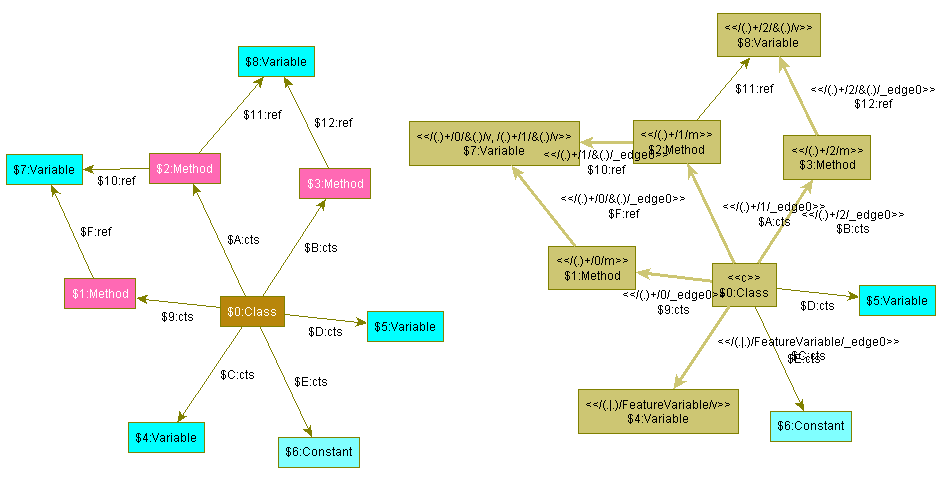
\includegraphics[width=\linewidth]{fig/exnested}}
\end{center}

The image from above shows an example how a structure is matched by several pieces.
At the left, the plain host graph, at the right with the match of \texttt{classWithStuff} inscribed.

\begin{grgen}
test classWithStuff
{
  c:Class; // get a class
	
  multiple { // get all of its methods, expect at least one
    c --> m:Method;
		independent { // expect an argument variable
		  m -:ref-> v:Variable;
		}
  }	

  alternative // additionally, match one of either
  {
    FeatureVariable { // a variable
      c --> v:Variable;
    }
    FeatureConstant { // or a constant
      c --> ct:Constant;
    }
  }
}
\end{grgen}

The example matches a class node \texttt{c} and its contained methods with a \texttt{multiple} pattern -- note the 3 instances of the pattern in the host graph getting captured by the single pattern description
(\verb#/(.)+/1/m# reads as multiple pattern (see Table~\ref{keywordregexpsyntax} explaining the regular expression syntax), match instance \texttt{1} (starting at \texttt{0}), pattern element \texttt{m}.)

Additionally, one of the alternative cases of a variable or a constant is matched -- here we got two potential patterns, from which only one is matched, capturing node \verb#$4# out of the potential targets \verb#$4#, \verb#$5#, \verb#$6#
(\verb#/(.|.)/FeatureVariable/v# reads as alternative, case \texttt{FeatureVariable}, pattern element \texttt{v}.)

The independent that is used to reference a parameter variable \texttt{v} from method \texttt{m} allows to re-match an already matched variable that would be otherwise shut out from getting matched again
(happened here with node \verb#$7#, matched from instances $0$ and $1$ of the multiple pattern; a graph element is annotated with all matching pattern elements).

\end{example}



%%%%%%%%%%%%%%%%%%%%%%%%%%%%%%%%%%%%%%%%%%%%%%%%%%%%%%%%%%%%%%%%%%%%%%%%%%%%%%%%%%%%%%%%%%%%%%%%
\section{Nested Pattern Rewriting}
\indexmain{nested pattern rewrite}\label{sec:nestedrewrite}

Until now we focused on the pattern matching of nested and subpatterns -- but we're not only interested in finding patterns combined from several pattern pieces, we want to rewrite the pattern pieces, too.
So we will extend the language of the structure parser introduced so far into a language for a structure transducer.
This does not hold for the application conditions, which are pure conditions, but for all the other language constructs introduced in this chapter.

\begin{rail}  
  NestedRewriting: ('replace' | 'modify') lbrace (()+RewriteStatement) rbrace;
\end{rail}\ixnterm{NestedRewriting}\ixkeyw{replace}\ixkeyw{modify}

Syntactically the rewrite is specified by a modify or replace clause nested directly within the scope of each nested pattern;
in addition to the rewrite clause nested within the top level pattern.
Semantically for every instance of a pattern piece matched its dependent rewrite is applied. 
So in the same manner the complete pattern is assembled from pattern pieces, the complete rewrite gets assembled from rewrite pieces
(or operationally: rewriting is done along the match tree by rewriting one pattern piece after the other).
Note that \texttt{return} statements are not available as in the top level rewrite part of a rule, and the \texttt{exec} statements are slightly different.

For a static pattern specification like the iterated block yielding dynamically a combined match of zero to many pattern matches, every submatch is rewritten, according to the rewrite specification applied to the host graph elements of the match bound to the pattern elements
(if the pattern was matched zero times, no dependent rewrite will be triggered - but note that zero matches still means success for an iterated, so the dependent rewrite piece of the enclosing pattern will be applied).
This allows e.g. for reversing all edges in the iterated-example (denoting containment in the class), as it is shown in the first of the following two examples.
For the alternative construct the rewrite is specified directly at every nested pattern, i.e. alternative case as shown in the second of the following two examples); the rewrite of the matched case will be applied.

Nodes and edges from the pattern containing the nested pattern containing the nested rewrite are only available for deletion or retyping inside the nested rewrite if it can be statically determined this is unambiguous, i.e. only happening once.
So only the rewrites of alternative cases, optional patterns or subpatterns may contain deletions or retypings of elements not declared in their pattern (in contrast to iterated and multiple pattern rewrites).

\begin{example}
%This is an example for a rewrite part nested within an iterated block. - without the comment the two examples fit on one page
  \begin{grgen}
rule methods
{
  c:Class;
  iterated {
    c --> m:Method;

    replace {
      c <-- m;
    }
  } 

  replace {
    c;
  }  
}
  \end{grgen}
\end{example}

\begin{example}
%This is an example for a rewrite parts nested within alternative cases. - without the comment the two examples fit on one page
  \begin{grgen}
rule methodWithTwoOrThreeParameters(m:Method)
{
  alternative {
    Two {
      m <-- n:Name;
      m <-e1:Edge- v1:Variable;
      m <-e2:Edge- v2:Variable;
      negative {
        v1; v2; m <-- :Variable;
      }

      modify {
        delete(e1); m --> v1;
        delete(e2); m --> v2;	    
      }
    }
    Three {
      m <-- n:Name;
      m <-e1:Edge- v1:Variable;
      m <-e2:Edge- v2:Variable;
      m <-e3:Edge- v3:Variable;

      modify {
        delete(e1); m --> v1;
        delete(e2); m --> v2;
        delete(e3); m --> v3;
      }
    }

  //modify { can be omitted - see below
  //}
}
  \end{grgen}
\end{example}

\begin{note} \label{omitmodify}
In case you got a \texttt{rule} or \texttt{pattern} with an empty \texttt{modify} clause, with all the real work going on in an \texttt{alternative} or an \texttt{iterated}, you can omit the empty \texttt{modify} clause.
This is a small syntactic convenience reducing noise which is strictly restricted to the top level pattern --- omitting rewrite parts of nested patterns specifies the entire pattern to be match-only (like a \texttt{test}; this must be consistent for all nested patterns).
\end{note}

\begin{example}
This is an example which shows how to decide with an alternative on the target type of a retyping depending on the context.
Please note the omitted rewrite (cf. \ref{omitmodify}).

  \begin{grgen}
rule alternativeRelabeling
{
  m:Method;
  
  alternative {
    private {
      if { m.access == Access::private; }

      modify {
        pm:PrivateMethod<m>;
      }
    }
    static {
      negative {
        m <-- c;
      }

      modify {
        sm:StaticMethod<m>;
      }
    }
  } 
}
  \end{grgen}
\end{example}


\chapter{Subpatterns and Yielding}\indexmain{subpatterns}
\label{cha:sub}

After the introduction of the nested patterns in chapter \ref{cha:nested} we will now have a look at the subpatterns, with the split into subpattern declaration plus subpattern entity declaration and subrule declaration plus usage, the other means to greatly enhances the flexibility and expressiveness of pattern matching and rewriting.

%%%%%%%%%%%%%%%%%%%%%%%%%%%%%%%%%%%%%%%%%%%%%%%%%%%%%%%%%%%%%%%%%%%%%%%%%%%%%%%%%%%%%%%%%%%%%%%%
\section{Subpattern Declaration and Subpattern Entity Declaration}
\indexmain{subpattern}\label{sec:subpattern}

Subpatterns were introduced to factor out a common recurring pattern -- a shape -- into a named subpattern type, ready to be reused at points the pattern should get matched.
The common recurring pattern is specified in a subpattern declaration and used by a subpattern entity declaration.

\begin{rail}  
  SubpatternDeclaration: 
    'pattern' IdentDecl Parameters? (('modify'|'replace') Parameters)? \\
	lbrace SubpatternBody rbrace ;
  SubpatternBody: (PatternStatement+) SubpatternRewriting?;
\end{rail}\ixkeyw{pattern}\ixkeyw{modify}\ixkeyw{replace}\ixnterm{SubpatternDeclaration}\ixnterm{SubpatternBody}\label{subpatterndecl}\indexmain{subpattern declaration}

Subpattern declarations define a subpattern type denoting the specified shape in the global namespace;
the parameters specify some context elements the pattern may refer to, but which are not part of the pattern itself. 
So they are only syntactically the same as test/rule-parameters (which are members of the pattern part).
A further difference is the lack of \emph{ReturnTypes}; they are not actions, just a helper in constructing complex patterns.
In order to get values out they employ the language construct of def entities which are yielded to (cf. \ref{sec:localvarorderedevalyield} later in this chapter).
Subpatterns can receive additional rewrite parameters, in addition to the pattern parameters, in contrast to the actions; they can be used to hand in nodes which are created in the rewrite part of the action or subpattern which contains the subpattern entity.
(The nested body will be explained in Section~\ref{sec:subrule}.)

\begin{rail}  
  SubpatternEntityDeclaration: 
    Ident ':' SubpatternType '(' ((Ident|Expression) * ',') ')' ';' ;
\end{rail}\ixnterm{SubpatternEntityDeclaration}\indexmain{subpattern entity declaration}

Subpattern entity declarations instantiate an entity of the subpattern type (i.e. specified shape), which means the subpattern must get matched for the matching of the enclosing pattern to succeed.
The arguments given are bound to the corresponding parameters of the subpattern.
If you prefer a syntactical point of view, you may see the subpattern entity as a placeholder, which gets substituted in place by the textual body of the subpattern declaration under renaming of the parameters to the arguments.
If you prefer an operational point of view, you may see the subpattern entity as a call to the matcher routine searching for the specified pattern from the given arguments on (constructing a match piece, which is the base for rewriting of that part).

%TODO:remove
%Termersetzung mit Termen die Graphen beschreiben.
%Mehrelementige Graphsprachen als Zwischenschritt zu den rekursiven bereits mit alternative... eingef�hrt -- dort auch so erkl�rt, wirklich eingef�hrt? vor rekursiv trotzdem noch ein  Zwischenschritt: pattern mit alternative, statt action mit alternative

\begin{example}
  \begin{grgen}
pattern TwoParameters(mp:Method)
{
  mp <-- :Variable;
  mp <-- :Variable;
}
test methodAndFurther
{
  m:Method <-- n:Name;
  tp:TwoParameters(m);
}
  \end{grgen}

  In the given example a subpattern \texttt{TwoParameters} is declared, connecting the context element \texttt{mp} via two edges to two variable nodes.
  The test \texttt{methodAndFurther} is using the subpattern via the declaration of the entity \texttt{tp} of type \texttt{TwoParameters}, binding the context element to its local node \texttt{m}.
  The resulting test after subpattern derivation is equivalent to the test \texttt{methodWithTwoParameters}.

  \begin{grgen}
test methodWithTwoParameters
{
  m:Method <-- n:Name;
  m <-- :Variable;
  m <-- :Variable;
}
  \end{grgen}
\end{example}

%-----------------------------------------------------------------------------------------------
\subsection{Recursive Patterns}\indexmain{recursive pattern}\indexmain{structural recursion}

Subpatterns can be combined with alternative patterns or the cardinality patterns into recursive subpatterns, i.e. subpatterns which may contain themselves.
Subpatterns containing themselves alone -- directly or indirectly -- would never yield a match as an infinite pattern can't be found in a limited graph.

\begin{example}\label{exiterpath}
  \begin{grgen}
test iteratedPath
{
  root:Assign;
  negative { --> root; }
  :IteratedPath(root); // match iterated path = assignment list
}

pattern IteratedPath(prev:Node)
{
  optional { // nothing or a linked assignment and again a list
    prev --> a:Assign; // assignment node 
    :IteratedPath(a); // next one, plz
  }
}
  \end{grgen}
  
The code above searches an \indexed{iterated path} from the root node on, here an assignment list. 
The iterated \indexed{path} with the optional is equivalent to the code below. Note the negative which ensures you get a longest match -- without it the empty case may be chosen lazily just in the beginning.
Please note that if you only need to check for the existence of such a simple iterated path you can use the \texttt{reachable} functions, or even better \texttt{isReachable} predicates introduced in \ref{transitiveneighbour}.

  \begin{grgen}
pattern IteratedPath(prev:Node)
{
  alternative {
    Empty {
      negative {
        prev --> a:Assign;
      }
    }
    Further {
      prev --> a:Assign;
      :IteratedPath(a);
    }
  }
}
  \end{grgen}

The code below searches an iterated path like the code above, just that it stops when a maximum length is reached.
The \indexed{bounded iterated path} is realized by 
calling a pattern with the requested maximum depth,
counting the depth parameter down with each recursion step,
until the limit checked by a condition is reached.
The \texttt{boundedReachable} functions introduced in \ref{transitiveneighbourbounded} should be preferred in a simple case like this.

  \begin{grgen}
test boundedIteratedPath(root:Assign)
{
  :BoundedIteratedPath(root, 3); // match iterated path of depth 3
}

pattern BoundedIteratedPath(prev:Node, var depth:int)
{
  optional { // nothing or a linked assignment and again a list
    prev --> a:Assign; // assignment node 
    :IteratedPath(a, depth-1); // next one, plz
    if{ depth >= 1; } // stop when we have reached max depth
  }
}
  \end{grgen}
\end{example}

\begin{example}
  \begin{grgen}
rule removeMiddleAssignment
{
  a1:Assign --> a2:Assign --> a3:Assign;
  independent {
    :IteratedPath(a1,a3)
  }
  
  replace {
    a1; a3;
  }
}

pattern IteratedPath(begin:Assign, end:Assign)
{
  alternative { // an iterated path from begin to end is either
    Found { // the begin assignment directly linked to the end assignment (base case)
      begin --> end;
    }
    Further { // or an iterated path from the node after begin to end (recursive case)
      begin --> intermediate:Assign;
      :IteratedPath(intermediate, end);
    }
  }
}
  \end{grgen}

This is once more a fabricated example, for an iterated path from a source node to a distinctive target node, and an example for the interplay of subpatterns and positive application conditions to check complex conditions independent from the pattern already matched.
Here, three nodes \texttt{a1},\texttt{a2},\texttt{a3} of type \texttt{Assign} forming a list connected by edges are searched, and if found, \texttt{a2} gets deleted, but only if there is an iterated path of directed edges from \texttt{a1} to \texttt{a3}.
The path may contain the host graph node matched to \texttt{a2} again.
Without the \texttt{independent} this would not be possible, as all pattern elements -- including the ones originating from subpatterns -- get matched isomorphically. 
The same path specified in the pattern of the rule -- not in the independent -- would not get matched if it would go through the host graph node matched to b, as it is locked by the isomorphy constraint.
Again, the \texttt{reachable} functions and \texttt{isReachable} predicates introduced in \ref{transitiveneighbour} are the better choice here.
They always match independently from the patterns (so when you need locking, you cannot employ them), can be used directly, and are implemented (more) efficiently. 
\end{example}

With recursive subpatterns you can already capture neatly structures extending into depth (as iterated paths)
and also structures extending into breadth (as forking patterns, although the cardinality statements are often much better suited to this task).
But combined with an iterated block, you may even match structures extending into breadth and depth,
like e.g. an inheritance hierarchy of classes in our example domain of program graphs, see example \ref{exsptree}, i.e. you can match a \indexed{spanning tree} in the graph.
This gives you a very powerful and flexible notation to capture large, complex patterns
built up in a structured way from simple, connected pieces (as e.g. abstract syntax trees of programming languages). 

\begin{note}
If you are working with hierarchic structures like that, 
you might be interested in the capabilities of GrShell/yComp for nested layout
as described and shown in \ref{sub:visual}/\ref{note:visual}).
\end{note}

\begin{example}\label{exsptree}
  \begin{grgen}
pattern SpanningTree(root:Class)
{
  iterated {
    root <-:extending- next:Class;
    :SpanningTree(next);
  }
}
  \end{grgen}
\end{example}

\begin{example}

\begin{center}
  \parbox{0.99\linewidth}{\includegraphics[width=\linewidth]{fig/exdepthbreadth}}
\end{center}

The image from above visualizes the matching of structures extending into depth and splitting into breadth, employing the pattern of test \texttt{db} from below.

\begin{grgen}
test db(root:Node)
{
  iterated {
    root --> child:N;
  }	
  dbc:chain(root);
}
pattern chain(begin:Node)
{
  alternative {
    again {
      begin --> next:Node;
      c:chain(next);
    }
    end {
      negative { begin --> .; }
    }
  }
}
\end{grgen}

\end{example}

\begin{example}

The example from the previous page utilizes the nested and subpatterns introduced in this and the previous chapter;
it matches \texttt{db} from a \texttt{root} node handed in on, in a tiny example graph (built from nodes of types \texttt{Node} and \texttt{N}, and edges of type \texttt{Edge}). 

The breadth-splitting structure is collected with an \texttt{iterated} pattern around the center node bound to the pattern node \texttt{root}.
The graph elements are annotated in the debugger (cf. Chapter~\ref{chapdebugger}) as usual with their pattern element name -- plus the (sub)pattern nesting path that lead to the instance of this pattern.

The \verb#(.)*/1/child# at the middle-right node tells that the node is contained in an iterated pattern (using the regular expression syntax for the iterated, see Table~\ref{keywordregexpsyntax}), that this is instance \texttt{1} (starting at \texttt{0}, here we got 3 matches of the iterated, so ending at instance count \texttt{2}, and that the name of the element in the pattern is \texttt{child}.

The depth-extending structure is collected with a subpattern \texttt{chain} employed from the test with the instance \texttt{dbc} starting at the node bound to the pattern node \texttt{root}.
It uses itself recursively with the subpattern instance \texttt{c}, from the node \texttt{next} on, which is reached with one edge-following-step from the input node \texttt{begin} on.

The \verb#/dbc/(.|.)/again/next# at the middle node of the chain tells that the node was matched on the subpattern instance named \texttt{dbc}, in an alternative (using regular expression syntax for the alternative), in the pattern of the \texttt{again} case, to the pattern node named \texttt{next}.
The same node is annotated with an\verb#/dbc/(.|.)/again/c/begin#, which stems from the fact that the node appears also in the next nesting step (subpattern call), in the instance \texttt{c} of the subpattern instantiated in the branch \texttt{again}; as \texttt{begin} node handed in to \texttt{chain}.

Breadth-splitting structure-matching is typically following \texttt{contains} edges, while depth-extending structure-matching is typically following \texttt{next} edges, please take a look at the Hints on Modeling~\ref{modelcontainsnext}. 

The (sub)pattern nesting paths can get long, cluttering display, so from a certain size on, only the size of the path is printed in the debugger. 

\end{example}

%%%%%%%%%%%%%%%%%%%%%%%%%%%%%%%%%%%%%%%%%%%%%%%%%%%%%%%%%%%%%%%%%%%%%%%%%%%%%%%%%%%%%%%%%%%%%%%%
\section{Subpattern Rewriting}
\indexmain{subrule}\label{sec:subrule}

Alongside the separation into subpattern declaration and subpattern entity declaration, 
subpattern rewriting is separated into a nested rewrite specification given within the subpattern declaration defining how the rewrite looks like 
and a subpattern rewrite application given within the rewrite part of the pattern containing the subpattern entity declaration requesting the rewrite to be actually applied.

\pagebreak

\begin{rail}  
  SubpatternRewriting: ('replace' | 'modify') lbrace (()+RewriteStatement) rbrace;
\end{rail}\ixnterm{SubpatternRewriting}\ixkeyw{replace}\ixkeyw{modify}

The subpattern rewriting specifications within the subpattern declaration looks like a nested rewriting specification,
but additionally there may be rewrite parameters given in the subpattern header (cf. \ref{subpatterndecl}) which can be referenced in the rewrite body.
(Most elements can be handed in with normal parameters, but elements created in the rewrite part of the user of the subpattern can only be handed in at rewrite time.) 

\begin{rail}  
  SubpatternRewriteApplication: 
    Ident '(' (Ident * ',') ')' ';' |
    SubpatternOccurence |
    SubpatternExecEmit
	;
\end{rail}\ixnterm{SubpatternRewriteApplication}

\noindent The \emph{SubpatternRewriteApplication} is part of the \emph{RewriteStatement} already introduced (cf. \ref{replstmt}).
The subpattern rewrite application is given within the rewrite part of the pattern containing the subpattern entity declaration,
in call notation on the declared subpattern identifier.
It causes the rewrite part of the subpattern to get used; if you leave it out, the subpattern is simply kept untouched.
The \emph{SubpatternOccurence} is explained in the next subsection \ref{sub:delpressub}.
The \emph{SubpatternExecEmit} is explained in chapter \ref{cha:imperativeandstate}.

\pagebreak

\begin{example}
This is an example for a subpattern rewrite application.

  \begin{grgen}
pattern TwoParametersAddDelete(mp:Method)
{
  mp <-- v1:Variable;
  mp <-- :Variable;

  modify {
    delete(v1);
    mp <-- :Variable;
  }
}
rule methodAndFurtherAddDelete
{
  m:Method <-- n:Name;
  tp:TwoParametersAddDelete(m);

  modify {
    tp(); // trigger rewriting of the TwoParametersAddDelete instance
  }
}
  \end{grgen}
\end{example}


\begin{example}
This is another example for a subpattern rewrite application,
reversing the direction of the edges on an iterated path.

  \begin{grgen}
pattern IteratedPathReverse(prev:Node)
{
  optional {
    prev --> next:Node;
    ipr:IteratedPathReverse(next);
    
    replace {
      prev <-- next;
      ipr();
    }
  }

  replace {
  }
}
  \end{grgen}
\end{example}

\begin{example}
This is an example for rewrite parameters, connecting every node on an iterated path to a common node (i.e. the local rewrite graph to the containing rewrite graph).
It can't be simulated by subpattern parameters which get defined at matching time because the common element is only created later on, at rewrite time.

  \begin{grgen}
pattern ChainFromToReverseToCommon(from:Node, to:Node) replace(common:Node)
{
  alternative {
    rec {
      from --> intermediate:Node;
      cftrtc:ChainFromToReverseToCommon(intermediate, to);

      replace {
        from <-- intermediate;
        from --> common;
        cftrtc(common);
      }
    }
    base {
      from --> to;

      replace {
        from <-- to;
        from --> common;
        to --> common;
      }
    }
  }

  replace {
    from; to;
  }
}
  \end{grgen}

  \begin{grgen}  
rule chainFromToReverseToCommon()
{
  from:Node; to:Node;
  cftrtc:ChainFromToReverseToCommon(from, to);

  modify {
    common:Node;
    cftrtc(common);
  }
}
  \end{grgen}
\end{example}

%-----------------------------------------------------------------------------------------------
\subsection{Deletion and Preservation of Subpatterns}\label{sub:delpressub}

In addition to the fine-grain dependent rewrite, subpatterns may get deleted or kept as a whole.

\begin{rail}  
  SubpatternOccurence: 
    Ident ';' |
    'delete' '(' (Ident + ',') ')' ';';
\end{rail}\ixkeyw{SubpatternOccurence}\ixkeyw{delete}

In modify mode, they are kept by default, but deleted if the name of the declared subpattern entity is mentioned within a delete statement.
In replace mode, they are deleted by default, but kept if the name of the declared subpattern entity is mentioned (using occurrence, same as with nodes or edges).

\begin{example}
  \begin{grgen}
rule R {
  m1:Method; m2:Method;
  tp1:TwoParameters(m1);
  tp2:TwoParameters(m2);

  replace {
    tp1; // is kept
    // tp2 not included here - will be deleted
    // tp1(); or tp2(); -- would apply dependent replacement
    m1; m2;
  }
}
  \end{grgen}
\end{example}

\begin{note}
You may even give a SubpatternEntityDeclaration within a rewrite part which causes the subpattern to be created; 
but this employment has several issues which can only be overcome by introducing explicit creation-only subpatterns
-- so you better only use it if you think it should obviously work (examples for the issues are alternatives -- which case to instantiate? -- and abstract node or edge types -- what concrete type to choose?). 

  \begin{grgen}
pattern ForCreationOnly(mp:Method)
{
  // some complex pattern you want to instantiate several times 
  // connecting it to the mp handed in
}
rule createSubpattern
{
  m:Method;
  
  modify {
    :ForCreationOnly(m); // instantiate pattern ForCreationOnly
  }
}
  \end{grgen}
\end{note}


%%%%%%%%%%%%%%%%%%%%%%%%%%%%%%%%%%%%%%%%%%%%%%%%%%%%%%%%%%%%%%%%%%%%%%%%%%%%%%%%%%%%%%%%%%%%%%%%
\section{Local Variables, Ordered Evaluation, and Yielding Outwards} \label{sec:localvarorderedevalyield}\indexmain{local variable}\indexmainsee{evalhere}{ordered evaluation}\indexmain{yielding outwards}

\subsection*{Local Variables and Ordered Evaluation} 
Sometimes attribute evaluation becomes easier with temporary variables;
such local variables can be introduced on a right hand side employing the known variable syntax \texttt{var name:type}, prefixed with the \texttt{def}\indexmain{def} keyword.
From then on they can be read and assigned to in eval statements of the RHS, or used as variable parameters in subpattern rewrite calls.
In addition, on their introduction an initializing expression may be given.

\begin{example}
  \begin{grgen}
rule R {
  n1:N; n2:N; n3:N; n4:N; n5:N;
  
  modify {
    def var mean:double = (n1.v + n2.v + n3.v + n4.v + n5.v)/5;
    eval {
    	n1.variance = (n1.v - mean)*(n1.v - mean); 
    	n2.variance = (n2.v - mean)*(n2.v - mean); 
    	n3.variance = (n3.v - mean)*(n3.v - mean); 
    	n4.variance = (n4.v - mean)*(n4.v - mean); 
    	n5.variance = (n5.v - mean)*(n5.v - mean); 
    }
  }
}
  \end{grgen}
\end{example}


Normally the rewrite order is as given in table \ref{table:executionorderrewriting}:
\begin{table}[htbp]
  \centering
  \begin{tabularx}{\linewidth}{|l|X|} \hline
    \texttt{ 1. } & \texttt{ Extract elements needed from match } \\
    \texttt{ 2. } & \texttt{ Create new nodes } \\
    \texttt{ 3. } & \texttt{ Call rewrite code of used subpatterns} \emph{and more...} \\ 
	  \texttt{ 4. } & \texttt{ Call rewrite code of nested iterateds } \\
    \texttt{ 5. } & \texttt{ Call rewrite code of nested alternatives } \\
    \texttt{ 6. } & \texttt{ Redirect edges } \\  
    \texttt{ 7. } & \texttt{ Retype (and merge) nodes } \\  
    \texttt{ 8. } & \texttt{ Create new edges } \\
    \texttt{ 9. } & \texttt{ Retype edges } \\  
    \texttt{ 10. } & \texttt{ Create subpatterns } \\
    \texttt{ 11. } & \texttt{ Attribute reevaluation } \\
    \texttt{ 12. } & \texttt{ Remove edges } \\ 
	  \texttt{ 13. } & \texttt{ Remove nodes } \\
    \texttt{ 14. } & \texttt{ Remove subpatterns } \\
    \texttt{ 15. } & \texttt{ Emit / Exec } \\  
    \texttt{ 16. } & \texttt{ Return } \\ \hline
	\end{tabularx}
	{\small \emph{and more...} at \texttt{3.} are \texttt{evalhere}, \texttt{emithere}, \texttt{alternative} Name, \texttt{iterated} Name}
  \caption{Execution order rewriting}
  \label{table:executionorderrewriting}
\end{table}

So first the subpatterns rewrites, then the iterated rewrites, then the alternative rewrites are executed, and finally the local eval statements (computations).
This might be sufficient in some cases, but in other cases when you want to compute an attributation over a tree/a graph, you want to have local computations influenced by attributes in nested/called children or its siblings, and attributes in nested/called children influenced by its parents or siblings.
So we need a language device which allows us to intermingle attribute computations in between the rewrite part executions of nested patterns and subpattern rewrite calls.
And a language device which allows us to give the execution oder of the alternative and iterated statements relative to the subpattern rewrite calls and attribute evaluations.

To achieve attribute evaluation in a defined order in between the subpattern rewrite calls, we use ordered evaluation statements, introduced with the keyword \texttt{evalhere}; 
they get executed in the order in which they are given syntactically
(a further statement executed in order is \texttt{emithere}, introduced in \ref{sec:deferredexecemithere}).

To achieve iterated/alternative execution in order, we allow names to be given to nested patterns, and reuse this name in a nested pattern rewrite order specification.
Naming nested patterns is done with the following syntax, as the already introduced syntax remains valid, on aggregate we extend the nested patterns with optional names to form \indexed{named nested pattern}.

\begin{rail}  
  NamedNestedPattern: 
    ('negative' | 'independent') IdentDecl lbrace etc rbrace;
    ('iterated' | 'multiple' | 'optional') IdentDecl etc rbrace;
    'alternative' IdentDecl lbrace etc rbrace;
\end{rail}

Alternatives and iterateds named this way can then be referenced in the rewrite part with an alternative rewrite order specification or an iterated rewrite order specification.

\begin{rail}  
  CardinalityRewriteUsage: 
    ('iterated' | 'multiple' | 'optional') Ident ';';
  AlternativeRewriteUsage: 
    'alternative' Ident ';';
\end{rail}

What we've seen so far is applied in the following example.
A \texttt{yield} prefix is needed whenever a \texttt{def} variable is written to (as  assignment target as well as a subpattern output argument). 

\begin{example}
  \begin{grgen}
rule R {
  iterated foo { .; modify { ..read i.. } }
  alternative bar { case { modify { ..read i.. } } } 
  sub1:Subpattern1();
  sub2:Subpattern2();

  modify {
    def var i:int = 0; // initializes i to 0
    evalhere { yield i = i + 1; } // afterwards i==1
    sub1(i); // input 1 to subpattern rewrite
    evalhere { yield i = i + 1; } // afterwards i==2
    iterated foo; // nested iterated reads i==2 
    evalhere { yield i = i + 1; } // afterwards i==3
    alternative bar; // nested alternative reads i==3
    evalhere { yield i = i + 1; } // afterwards i==4
    sub2(i); // input 4 to subpattern rewrite
    evalhere { yield i = i + 1; } // afterwards i==5
    eval { yield j = i + 1; } // assign 6 to j
  }
}
  \end{grgen}
\end{example}

\begin{note}
For rewriting the execution order of the parts can be defined, to allow programming attribute evaluation orders of interest, defining when to descend into which part and defining glueing/local computations in between.
(A depth first run with a defined order in between the siblings, comparable to an LAG/RAG run in compiler construction, but with an explicitly defined sequence of children visits, instead of a temporal succession implicitly induced by the syntactical left-to-right ordering).
In contrast to rewriting, the \emph{matching} order of the pattern parts can \emph{not} be defined, to allow the compiler/the runtime to use the evaluation order it estimates to be the best.
So we can't access attributes from sibling elements, we can only compute attributes top down from local elements or elements handed in on matching, and later on bottom up from local elements or elements bubbling up at match object tree construction.
Top down attribute evaluation operates on the already matched elements and attribute values or the ones received as inputs, which are handed down implicitly into nested patterns or explicitly via subpattern parameters into subpattern instances. (A depth first run too, but without a defined order in between the siblings, comparable to an IAG run in compiler construction for computing inherited attributes during matching while descending).
Bottom up attribute evaluation operates on the matched elements and attribute values locally available or the ones received into def elements yielded implicitly upwards from the nested patterns or explicitly accumulating iterated results or with assigning out parameters of subpatterns. (The same depth first run, but with attributes computed while ascending, comparable to an SAG run in compiler construction for computing synthesized attributes.)
\end{note}

\subsection*{Yielding Outwards During Rewriting}\label{sub:yield} 

Sometimes one needs to bring something matched within a nested or subpattern to an outer pattern containing it (nested patterns) or calling it (subpatterns).
So that one can do there (in the using pattern) operations on it, e.g. attaching a further edge to an end node of a chain matched with recursive patterns (thus modularizing the graph rewrite specification into chain matching patterns and patterns using chains doing things on the chain ends), or summing attributes matched in iterated pattern instances. 

The first thing one needs to bring something outwards is a target in a nesting or calling pattern. 
This is achieved by nodes, edges, and variables declared with the \texttt{def} keyword in a rewrite part, marking them as output entities;
variables were already introduced in previous paragraphs, but in addition to them nodes and edges are allowed, too.
Furthermore subpattern rewrite parameters may be declared as def parameters,
marking them as output parameters.
These elements are then yielded to from within \texttt{eval} or \texttt{evalhere} statements, subpattern rewrite usages, and \texttt{exec} statements.
While the latter will be covered in chapter \ref{cha:imperativeandstate}, the former will be explained in the following.

Yielding is specified by prepending the \texttt{yield}\indexmain{yield} keyword to the entity yielded to,
in an assignment to a variable or a method call on a variable,
inside an \texttt{eval} or \texttt{evalhere}-statement, or a change assignment; 
the target of the assignment may be a node or edge (if declared as output variable).
The yield must be prepended to the argument for a subpattern def rewrite parameter, too.

\begin{example}
  \begin{grgen}
pattern Chain(begin:Node) modify(def end:Node)
{
  alternative {
    Further {
      begin --> intermediate:Node;
      c:Chain(intermediate);
      
      modify {
        c(yield end);
      }
    }
    Done {
      negative {
        begin --> ;
      }
      
      modify {
        eval {
          yield end = begin;
        }
      }
    }
  }
  
  modify { }
}

rule R(begin:Node) : (Node) {
  c:Chain(begin);

  modify {
    def end:Node;
    c(yield end); // end is filled with chain end
    return(end);
  }
}
  \end{grgen}
  First example for RHS yielding: returning the end node of a chain.
\end{example}

\begin{example}
  \begin{grgen}
rule outCount(head:Node) : (int)
{
  iterated {
    head --> .;
    modify {
      eval { yield cnt = cnt + 1; }
    }
  }

  modify {
    def var cnt:int = 0;
    return (cnt);
  }
}
  \end{grgen}
  Second example for RHS yielding: counting the number of edges matched with an iterated.
\end{example}

\subsection*{Yielding Outwards During Match Object Construction} 

Bubbling up the elements from nested patterns and called patterns during rewriting might be too late or inconvenient.
Luckily it can be done before, at the end pattern matching when the match object tree gets constructed.

As for RHS yielding the targets of the yielding must be nodes, edges, or variables declared with the \texttt{def} keyword prepended, marking them as output entities; but this time in the pattern part.
Furthermore subpattern parameters may be declared as def parameters in the subpattern definition header, marking them as output parameters.

These elements can then be yielded to from within \texttt{eval} statements inside a \texttt{yield} block
(maybe with iterated accumulation) and subpattern usages.
A \texttt{yield} block is a constrained \texttt{eval} block which can be given in the pattern part;
it does not allow to assign to or change non-\texttt{def} variables, or carry out graph-changing commands.
Yielding is specified by prepending the \texttt{yield}\indexmain{yield} keyword to the entity yielded to,
in the assignment or method call.
The \texttt{yield} must be prepended to the argument for a subpattern def parameter, too.

\begin{warning}
A def entity from the pattern part can't be yielded to from the rewrite part, they are constant after matching.
\end{warning}

Let's have a look at two examples for yielding:

\begin{example}
  \begin{grgen}
pattern Chain(begin:Node, def end:Node)
{
  alternative {
    further {
      begin --> next:Node;
      :Chain(next, yield end);
    }
    done {
      negative {
        begin --> ;
      }
      yield {
        yield end = begin;
      }
    }
  }
}

pattern LinkChainTo(begin:Node) modify(n:Node)
{
  alternative {
    further {
      begin --> next:Node;
      o:LinkChainTo(next);

      modify {
        next --> n;
        o(n);
      }
    }
    done {
      negative {
        begin --> ;
      }
		  
      modify {
      }
    }
  }

  modify { }
}

rule linkChainEndToStartIndependent(begin:Node) : (Node)
{
  def end:Node;
	
  independent {
    c:Chain(begin, yield end);
  }
  o:LinkChainTo(begin);
  	
  modify {
    o(end);
    return(end);
  }
}
  \end{grgen}
\end{example}

The first example for LHS yielding follows within an independent a chain piece by piece to some a priori unknown end node, and yields this end node chain piece by chain piece again outwards to the chain start. There it is used as input to another chain (maybe the same chain, maybe overlapping due to the independent), linking all the nodes of this chain to the end node of the former.

When yielding from an iterated pattern there's the problem that each yielding assignment from an iterated instance would overwrite the one def variable from outside the iterated, while one is interested most of the time in some accumulation of the values, e.g. summing integers or concatenating strings.
This can be achieved with a \texttt{for} loop iterating a def variable inside an iterated for all the matches of the iterated pattern referenced by name, allowing to assign to an outside def variable a value computed from the def variable and the value of the iterated def variable.

This is shown in the second example for LHS yielding, summing the integer attribute \texttt{a} of nodes of type \texttt{N} adjacent to a start node, matched with an iterated.

\begin{example}
  \begin{grgen}
test sumOfWeight(start:Node) : (int,int)
{
  def var sum:int = 0;
  def var v:int = 0;
	
  iterated it {
    def var i:int;
		
    start --> n:N; // node class N { a:int; }
		
    yield {
      yield i = n.a;
      yield v = 42; // v is assigned 42 multiple times
    }
  } 

  yield {
    for(i in it)
    {
      yield sum = sum + i;
    }
  }

  return (sum,v);
}
  \end{grgen}
\end{example}

In case no accumulation is needed but a simple \indexed{count} of the iterated matches is sufficient, one can employ the \texttt{count} operator on an iterated (that must have been named before), as displayed in the following example (the count is only available in a \texttt{yield} or \texttt{eval} block).

\begin{example}
  \begin{grgen}
test countOfEdges(start:Node) : (int)
{
  def var sum:int = 0;
	
  iterated it {
    start -->;
  } 

  yield {
    yield sum = count(it);
  }

  return (sum);
}
  \end{grgen}
\end{example}

%\pagebreak

%%%%%%%%%%%%%%%%%%%%%%%%%%%%%%%%%%%%%%%%%%%%%%%%%%%%%%%%%%%%%%%%%%%%%%%%%%%%%%%%%%%%%%%%%%%%%%%%
\section{Flow Example, Regular Expression Syntax, and Locking}\indexmainsee{EBNF}{regular expression syntax}\indexmain{regular expression syntax}\label{matchingflow}

Pattern matching and rewriting occurs in two completely distinct passes, separated by the part-pattern matches tree of the combined patterns.
During each pass, input and output parameters may be computed and passed; with explicit passing for subpatterns, and implicit passing for nested patterns (which can directly access the content of their contained pattern).

First the pattern is matched with recursive descent alongside pattern nesting and subpattern calling, employing some helper stacks in addition to the call stack (the pushdown machine is explained in more detail in \ref{sec:generatedcode}).
Matching occurs strictly top-down (or from the outside to the nested inside patterns), first the graphlets of the current pattern are matched, then control descends to the nested and subpatterns.
During matching, input parameters may be passed, esp. forwarding just matched elements or attributes from them; they allow to influence the matching process.

When a complete match is found, while ascending again, unwinding the call stack, output pattern-\texttt{def} parameters are passed bottom-up (or from the inside to the containing outside patterns) with \texttt{yield} blocks and \texttt{yield} assignments within those blocks, or \texttt{yield} bindings of \texttt{def} parameters in a subpattern call.
During this ascent, the part-pattern matches tree is assembled, each match of a pattern contains the matches of its nested patterns and used subpatterns when it is left.

In the rewrite step, the matches tree is visited recursively again, creating the new nodes of the current pattern, then descending to the nested patterns and subpatterns, executing their changes, and after they returned, executing all other changes of the pattern.
During this visit, rewrite input parameters may be passed, for forwarding just created elements (or computed values). 

On ascending again from a pattern, the rewrite-\texttt{def} elements are assigned from \texttt{yield} assignments in the \texttt{eval} blocks, or \texttt{yield} bindings of \texttt{def} rewrite parameters in a subpattern rewrite call.
(Technically, nested patterns are handled like subpatterns, with parameter passing for accessed elements of the containing pattern automatically inserted by the compiler.)

Let's take a look at an example, with Figure \ref{figmatchingparameterflow} depicting the input and output parameter passing during the matching of Example \ref{exmatchingparameterflow}, and Figure \ref{figrewritingparameterflow} depicting the input and output parameter passing during the rewriting of Example \ref{exrewritingparameterflow} (which is an extended version of Example \ref{figmatchingparameterflow}).

\begin{example}
  \begin{grgen}
rule r(a:Node) : (Node, int)
{
  a --> b:Node;
	
  def var i:int;
  optional o {
    a --> . --> c:N;
    yield { yield i = c.i; }
		
    modify {
    }
  }

  def d:Node;
  p:P(b, yield d);
	
  modify {
    b --> u:Node;
    return(d, i);
  }
}

pattern P(n:Node, def rm:Node)
{
  n --> . --> m:Node;
  yield { yield rm = m; }
}
  \end{grgen}
\end{example}\label{exmatchingparameterflow}

\begin{figure}[hptb]
  \centering
  \includegraphics[width=0.61\textwidth]{fig/MatchAndParameterFlowAnnotated}
  \caption{Parameter flow in matching}
  \label{figmatchingparameterflow}
\end{figure}

\begin{example}
  \begin{grgen}
rule r(a:Node) : (Node, int, Node, int) {
  a --> b:Node;
  def var i:int;
  optional o {
    a --> . --> c:N;
    yield {	yield i = c.i; }
		
    modify {
      eval { yield j = i + u.i; }
    }
  }
  def d:Node;
  p:P(b, yield d);
	
  modify {
    def e:Node; def var j:int;
    b --> u:N;
    p(u, yield e);
    return(d, i, e, j);
  }
}
pattern P(n:Node, def rm:Node) modify(k:Node, def x:Node) {
  n --> . --> m:Node;
  yield {	yield rm = m; }
	
  modify {
    m --> k; m --> l:Node;
    eval { yield x = l; }
  }
}
  \end{grgen}
\end{example}\label{exrewritingparameterflow}

\begin{figure}[hptb]
  \centering
  \includegraphics[width=0.63\textwidth]{fig/RewriteAndParameterFlowAnnotated}
  \caption{Parameter flow in rewriting}
  \label{figrewritingparameterflow}
\end{figure}

In Example \ref{exmatchingparameterflow}, a rule \texttt{r} is matched, which contains a nested \texttt{optional} pattern \texttt{o} and uses a subpattern \texttt{P}.
The rule matches from its input node \texttt{a} on a neighbouring node \texttt{b} and hands it in to the subpattern \texttt{p}.
In the optional pattern it matches a two-step neighbouring node \texttt{c} from \texttt{a} on.
The subpattern \texttt{P} matches from its input parameter \texttt{n} on a two-step neighbouring node \texttt{m}.

A \texttt{def} variable \texttt{i} is declared in the pattern, and \texttt{yield} assigned from the optional \texttt{o} an attribute of the \texttt{c} found there.
Another \texttt{def} variable \texttt{d} is declared in the pattern, and assigned from the subpattern call \texttt{p} with a \texttt{yield} parameter passing. 
The two pattern \texttt{def} variables are then \texttt{return}ed out of rule \texttt{r}.
The subpattern \texttt{P} \texttt{yield}s to its output \texttt{def} parameter \texttt{rm} the \texttt{m} found in its body.

In the extended Example \ref{exrewritingparameterflow}, the rewrite part of the rule \texttt{r} creates a node \texttt{u}, links it to \texttt{b}, and hands it in to the subpattern rewrite employment of \texttt{p}.
The rewrite part of subpattern \texttt{P} creates a node \texttt{l} and links it to \texttt{m}.
Additionally, an edge is inserted in between \texttt{m} and the rewrite input parameter \texttt{k}.

A \texttt{def} variable \texttt{j} is declared in the rewrite part of \texttt{r}, and \texttt{yield} assigned from the \texttt{eval} inside the rewrite part of the optional \texttt{o}.
Another \texttt{def} variable \texttt{e} is declared in the rewrite part, and assigned from the subpattern rewrite call \texttt{p}.
The two rewrite-\texttt{def} variables are then \texttt{return}ed out of the rule, in addition to the two pattern-\texttt{def} variables.
The subpattern \texttt{yield}s from its \texttt{eval} part to its output \texttt{def} rewrite parameter \texttt{x} the \texttt{l} just created.

Bottom line: you can flexibly combine patterns with nested and subpatterns, including input and output parameters.
You can pass parameters in during matching alongside matching order. When matching completed, during match-tree building, you can yield elements found in contained patterns out. 
When the rewrite is applied, you can pass parameters in alongside the buildup of the patterns, and yield elements out once more.
But not only are those two passes strictly distinct, but also are the parameter passing directions strictly distinct, first is all input parameter passing carried out during descent, then is all output parameter synthesizing carried out during ascent.


\subsubsection*{Regular Expression Syntax}
In addition to the already introduced syntax for the nested patterns with the keywords 
\texttt{negative}, \texttt{independent}, \texttt{alternative}, \texttt{iterated}, \texttt{multiple} and \texttt{optional},
there is a more lightweight syntax resembling regular expressions available; 
when used together with the subpatterns it yields graph rewrite specifications which look like EBNF-grammars with embedded actions. 
Besides reducing syntactical weight, they offer constructs for matching a pattern a bounded number of times (same notation as the one for the bounded iteration in the sequences).

%Table \ref{keywordregexpsyntax} lists the corresponding (/equivalent) language constructs; 
%Example \ref{introexampleregexp} is a version of the introductory example \ref{introexample} modified to use the new syntax. commented out to get better layout

\begin{table}[htbp]
  \centering
  \begin{tabularx}{\linewidth}{|l|X|} \hline
    \texttt{ iterated \{ P \} } & \texttt{ (P)* } \\
    \texttt{ multiple \{ P \} } & \texttt{ (P)+ } \\
    \texttt{ optional \{ P \} } & \texttt{ (P)? } \\ 
	\texttt{ alternative \{ l1 \{ P1 \} .. lk \{ Pk \} \} } & \texttt{ (P1|..|Pk) } \\
    \texttt{ negative \{ P \} } & \texttt{ $\sim$(P) } \\
    \texttt{ independent \{ P \} } & \texttt{ \&(P)} \\ \hline 
    \texttt{ modify \{ R \} } & \texttt{  \{+ R \} } \\
    \texttt{ replace \{ R \} } & \texttt{ \{- R \} } \\ \hline 
    \texttt{ - } & \texttt{ (P)[k] / (P)[k:l] / (P)[k:*] } \\ \hline 
	\end{tabularx}
  \caption{Map of nested patterns in keyword syntax to regular expression syntax}
  \label{keywordregexpsyntax}
\end{table}

Understanding \GrG-subpatterns may be easier given knowledge about EBNF-grammars when we compare them to those.
We find then that rules resemble grammar axioms, subpatterns resemble nonterminals, and graphlets resemble terminal symbols; nested patterns are similar to EBNF operators, and the rewrite part corresponds to the semantic actions of syntax directed translation.
Negative and independent patterns are used to explicitly check context constraints
(every graphlet as such is already able to match pieces that one would or could classify as context, graph rewriting allows for derivations that are highly adaptable to the surrounding parts).
See \cite{EBNFAGTIVE} for more on this.

  \begin{example}
    \begin{grgen}
test method
{
  m:Method <-- n:Name; // signature of method consisting of name
  ( m <-- :Variable; )* // and 0-n parameters
  
  :AssignmentList(m); // body consisting of a list of assignment statements
}

pattern AssignmentList(prev:Node)
{
  ( // nothing or a linked assignment and again a list
    prev --> a:Assign; // assignment node 
    a -:target-> v:Variable; // which has a variable as target 
    :Expression(a);  // and an expression which defines the left hand side 
    :AssignmentList(a); // next one, plz
  )?
}

pattern Expression(root:Expr)
{
  ( // expression may be a binary expression of an operator and two expresions
      root <-- expr1:Expr;
      :Expression(expr1);
      root <-- expr2:Expr;
      :Expression(expr2);
      root <-- :Operator;
  | // or a unary expression which is a variable (reading it)
      root <-- v:Variable;
  )
}
    \end{grgen}
  \end{example}\label{introexampleregexp}

\subsubsection*{Isomorphy Locking} \label{locking}
When matching a program graph as in the introductory example \ref{ex:proggraph} one might be satisfied with matching a tree structure.
But on other occasions one wants to match \emph{backlinks} and especially the targets of the backlinks, too, 
from \emph{uses} nested somewhere in the syntax graph to \emph{definitions} whose nodes were already matched earlier in the subpattern derivation (subpatterns can be seen as an equivalent of grammar rules known from parser generators).
Unfortunately these elements are already matched and thus isormorphy locked following the default semantics of isomorphic matching.
And unfortunately these elements can't be declared \texttt{hom}omorphic as they are unknown in the nested subpattern.
Handing them in as parameters and then declaring them \texttt{hom}omorphic is only possible if they are of a statically fixed number (as the number of parameters is fixed at compile time), which is normally not the case for e.g. the attributes of a class in a syntax graph.
In order to handle this case the \texttt{independent} \emph{operator} (cf. \ref{rule:homspec}) was added to the rule language
--- when you declare the backlink target node \texttt{n} as \texttt{independent(n)} it can be matched once again.
Thus it is possible to match e.g. a class attribute definition node which was already matched when collecting the attributes of the class again later on in a subpattern when matching an expression containing a usage of that attribute, allowing to e.g. add further edges to it.

\subsubsection*{Patternpath Locking} 
As stated in the sections on the negative and independent constructs (\ref{nac}, \ref{pac}), they get matched homomorphically to all already matched elements. By referencing an element from outside you can isomorphy lock that element to prevent it to get matched again.

Maybe you want to lock all elements from the directly enclosing pattern, in this case you can just insert \texttt{pattern;} in the position of a graphlet into the NAC or PAC.

Maybe you want to lock all elements from the patterns dynamically containing the NAC/PAC of interest, i.e. all subpattern usages and nesting patterns on the path leading to the NAC/PAC of interest (but not their siblings). In this case you can insert \texttt{patternpath;} in the position of a graphlet into the NAC or PAC. You might be interested in this construct when matching a piecewise constructed pattern, e.g. a chain, which requires to check for another chain (iterated path) which is not allowed to cross (include an element of) the original one.


%todo: quick reference table showing a pattern one is interested in and the language construct to capture it (breadth, alternativem, depth, ..)


\include{nestedandsubpatternrewriting}

\include{nestedandsubpatternyielding}

\chapter{Rule Application Control Language (Sequences)}\indexmain{rule application language}
\label{cha:xgrs}

Graph rewrite sequences (GRS)\indexmain{graph rewrite sequence}, better extended graph rewrite sequences XGRS, to distinguish them from the older graph rewrite sequences, are a domain specific \GrG~language used for controlling the application of graph rewrite rules. 
They are available
\begin{itemize}
\item as an imperative enhancement to the rule set language.
\item for controlled rule application within the \GrShell.
\item for controlled rule application on the API level out of user programs.
\end{itemize}

If they appear in rules, they get compiled, otherwise they get interpreted.
Iff used within \GrShell, they are amenable to debugging.

Graph rewrite sequences are built from a pure \emph{rule control} language,
written down in a syntax similar to boolean and regular expressions, with rule applications as atoms,
and a \emph{computations} sublanguage,
noted down as a sequence of assignments, function calls, or procedure calls.
A computation is given as an atom of the rule control language, nested in curly braces.

The graph rewrite sequences are a means of composing complex graph transformations out of single graph rewrite rules and further computations.
The control flow in the rule control language is determined by the evaluation order of the operands.
Graph rewrite sequences have a boolean return value; for a single rule, \texttt{true} means the rule was successfully applied to the host graph.
A \texttt{false} return value means that the pattern was not found in the host graph. 

In order to store and reuse return values of rewrite sequences and most importantly, 
for passing return values of rules to other rules, \emph{variables} can be defined.
A variable is an arbitrary identifier which can hold a graph element or a value of one of the attribute or value types \GrG\ knows.
There are two kinds of variables available in \GrG,
i) graph global variables\indexmain{graph global variable}\indexmainsee{variable}{graph global variable} and 
ii) sequence local variables\indexmain{sequence local variable}\indexmainsee{variable}{sequence local variable}.
A variable is alive from its first declaration on: graph global variables are implicitly declared upon first usage of their name,
sequence local variables are explicitly declared with a typed variable declaration of the form \texttt{name:type}.
Graph global variables must be prefixed with a double colon \texttt{::}, local variables are referenced just with their name.
Graph global variables are untyped; their values are typed, though, so type errors cause an exception at runtime.
They belong to and are stored in the graph processing environment -- if you save the graph in \GrShell\ 
then the variables are saved, too, and restored next time you load the saved graph.
Further on, they are nulled if the graph element assigned to them gets deleted (even if this happens due to a transaction rollback),
thus saving one from debugging problems due to zombie elements (you may use the \texttt{def()} operator to check during execution if this happened).
Sequence local variables are typed, so type errors are caught at compile time (parsing time for the interpreted sequences); 
an assignment of an untyped variable to a typed variable is checked at runtime.
They belong to the sequence they appear in, their life ends when the sequence finishes execution 
(so there is no persistence available for them as for the graph global variables; neither do they get nulled on element deletion as the graph does not know about them). 

If used in some rule, i.e. within an \texttt{exec}, named graph elements of the enclosing rule are available as read-only variables.

Note that we have two kinds of return values in graph rewrite sequences.
Every rewrite sequence returns a boolean value, indicating whether the rewriting could be successfully processed, i.e. denoting success or failure.
Additionally rules may return graph elements.
These return values can be assigned to variables on the fly (see example \ref{ex:grsreturn}).
\begin{figure}[htbp]
\begin{example}
	\label{ex:grsreturn}
The graph rewrite sequences
	\begin{grgen}	 
(b,c)=R(x,y,z)=>a
a = ((b,c)=R(x,y,z))
	\end{grgen}
assign the two returned graph elements from rule \texttt{R} to variables \texttt{b} and \texttt{c} and the information whether \texttt{R} mached or not to variable \texttt{a}. The first version is recommended.
\end{example}
\end{figure}


%%%%%%%%%%%%%%%%%%%%%%%%%%%%%%%%%%%%%%%%%%%%%%%%%%%%%%%%%%%%%%%%%%%%%%%%%%%%%%%%%%%%%%%%%%%%%%%%
\section{Rule Application} \label{sec:ruleapplication}

\begin{rail} 
  RewriteFactor: RuleExecution
     | SimpleVariableHandling
     | ExtendedControl
     | RewriteComputationUsage
	; 
\end{rail}\ixnterm{RewriteFactor}

Rewrite factors are the building blocks of graph rewrite sequences.
They are split into four major areas: rule (and sequence) application, simple variable handling, extended control, and sequence computation usages.
Here we start with the most import one, applying rules.
In section \ref{sec:simplevarhandling} we visit simple variable handling.
In section \ref{sec:extctrl} we have a look at advanced control, and in section \ref{sec:seqcomp} at the sequence computations.

\begin{rail}
  RuleExecution: (() | '(' (Variable+',') ')' '=') \\ (RuleModifier Rule | (RandomSelection)? '[' RuleModifier Rule ']' | 'count' '[' RuleModifier Rule ']' '=''>' Variable);
  RandomSelection: dollar (percent)? ( Variable | (Variable ',' (Variable | '*')) )?;
  RuleModifier: (() | percent) (() | '?');
  Rule: RuleIdent (() | '(' (Variable+',') ')') (FilterCalls)?;
\end{rail}\ixnterm{RuleExecution}\ixnterm{RandomSelection}\ixnterm{RuleModifier}\ixnterm{Rule}

The \emph{RuleExecution} clause applies a single rule or test.
In case of a rule, the first found pattern match will be rewritten.
Application will fail in case no match was found and succeed otherwise. 
Variables and named graph elements can be passed into the rule.
The returned graph elements can be assigned to variables again.
The rule modifier \texttt{?} switches the rule to a test, i.e.\ the rule application does not perform the rewrite part of the rule but only tests if a match exists.
The rule modifier \texttt{\%} is a multi-purpose flag. 
In the \GrShell\ (see Chapter~\ref{chapgrshell}) it dumps the matched graph elements to \texttt{stdout};
in \texttt{debug}-mode (see Chapter~\ref{chapdebugger}) it acts as a \indexed{break point} (which is its main use in fact);
you are also able to use this flag for your own purposes, when using \GrG\ via its API interface (see Section~\ref{sct:API}).
The filter calls (which allow e.g. to order the matches list and rewrite only the top ones, or to filter symmetric matches) are explained in \ref{sub:filters}.

The \emph{RuleExecution} clause can be applied to a defined sequence (cf. \ref{sec:sequencedefinition}), or an external sequence (cf. \ref{sub:extseq}), too.
Application will succeed or fail depending on the result of the body of the sequence definition called.
In case of success, the output variables of the sequence definition are written to the destination variables of the assignment. In case of failure, no assignment takes place, so sequence calls behave the same as rule calls.
The break point \texttt{\%} can be applied to a sequence call, but neither the \texttt{?} operator nor all braces (\texttt{[]}).

The square braces (\texttt{[]}) introduce a special kind of multiple rule execution:
Every pattern match produced by the rule will be rewritten;
if at least one was found, rule execution will succeed, otherwise it will fail. 
If \emph{Rule} returns values, the value of each rule application will be returned.
This happens in the form of an array, or better one array per return parameter, with type \verb#array<T># for return parameter type \verb#T#.
The return parameter arrays are filled with as many values as there were succeeding rule applications.

The \texttt{count}ed all bracketing \texttt{count[r]=>c} assigns the \indexed{count} of matches of rule \texttt{r} to the variable \texttt{c}, and applies \texttt{r} on all the matches.
With \texttt{count[?r]=>c} the matches are only counted, no rewrites are carried out.

The \indexed{random match selector} \texttt{\$v} searches for all matches and then randomly selects \texttt{v} of them to be rewritten (but at most as much as are available), with \texttt{\$[r1]} being equivalent to \texttt{anonymousTempVar=1 \& \$anonymousTempVar[r1]}.
Rule application will fail in case no match was found and succeed otherwise (the return values are of array type, as with all-bracketed rule calls, even in case only one match is requested). 
You may change the lower bound for success by giving a variable containing the value to apply before the comma-separated upper bound variable.
In case a lower bound is given the upper bound may be set to unlimited with the \texttt{*}.
An \texttt{\%} appended to the \texttt{\$} denotes a \indexed{choice point} 
allowing the user to choose the match to be applied from the available ones in the debugger (see Chapter ~\ref{chapdebugger}).

\begin{example}
The sequence \verb#(u,v)=r(x,y)# applies the rule \texttt{r} with input from the variables \texttt{x} and \texttt{y} on the host graph 
and assigns the return elements from the rule to the variables \texttt{u} and \texttt{v} (the parenthesis around the out variables are always needed, even if there's only one variable assigned to).
The sequence \verb#$[t]# determines all matches of the parameterless rule \texttt{t} on the host graph, then one of the matches is randomly chosen and executed.
Rule \texttt{r} applied with all-bracketing may look like \verb#(u:array<Node>,v:array<int>)=[r(x,y)]#, note the return value arrays, compared to a single application with \verb#(u:Node,v:int)=r(x,y)#.
\end{example}


%%%%%%%%%%%%%%%%%%%%%%%%%%%%%%%%%%%%%%%%%%%%%%%%%%%%%%%%%%%%%%%%%%%%%%%%%%%%%%%%%%%%%%%%%%%%%%%%
\section{Logical and Sequential Connectives}\label{sec:connectives}

\makeatletter

\begin{rail}
  RewriteSequence: 
    (RewriteNegTerm) (( (dollar (percent)?)? (ampersand | xorhat | '|' | doubleampersand | '||' | ';>' | '<;') RewriteNegTerm )*)
|    '(' RewriteSequence ')'
	;
  RewriteNegTerm: 
    ('!')? RewriteTerm ( ('=''>' | ampersand'>' | '|''>') Variable)?
	;
\end{rail}\ixnterm{RewriteSequence}\ixnterm{RewriteNegTerm}

A graph rewrite sequence consists of several rewrite terms linked by operators.
Table \ref{tbl:sequ:op} gives the priorities and semantics of the operators, priorities in ascending order.
Forcing execution order against the priorities can be achieved by parentheses.
The modifier \texttt{\$} changes the semantics of the following operator to randomly execute the left or the right operand first (i.e. flags the operator to act commutative);
usually operands are executed / evaluated from left to right if not altered by bracketing.
In contrast the sequences \texttt{s}, \texttt{t}, \texttt{u} in \texttt{s \$<op> t \$<op> u} are executed / evaluated in arbitrary order.
The modifier \texttt{\%} appended to the \texttt{\$} overrides the random selection by a user selection (cf. see Chapter~\ref{chapdebugger}, \indexed{choice point}s).

The assign-to operator \texttt{=>} optionally available at the end of the $RewriteNegTerm$ assigns the (negated in case of \texttt{!}) result of the $RewriteTerm$ execution to the given variable; the and-to \texttt{\&>} operator assigns the conjunction and the or-to \texttt{|>} operator assigns the disjunction of the original value of the variable with the sequence result to the variable.

\begin{table}[htbp]
    \begin{tabularx}{\linewidth}{l|X}
        \bf Operator & \bf Meaning \\\hline\hline
        \verb/s1 <; s2/ & Then-Left, evaluates \texttt{s1} then \texttt{s2} and returns(/projects out) the result of \texttt{s1}\\
		\verb/s1 ;> s2/ & Then-Right, evaluates \texttt{s1} then \texttt{s2} and returns(/projects out) the result of \texttt{s2}\\\hline
        \verb/s1 || s2/ & Lazy Or, the result is the logical disjunction, evaluates \texttt{s1}, only if \texttt{s1} is false \texttt{s2} gets evaluated\\\hline
        \verb/s1 && s2/ & Lazy And, the result is the logical conjunction, evaluates \texttt{s1}, only if \texttt{s1} is true \texttt{s2} gets evaluated\\\hline
        \verb/s1 | s2/ & Strict Or, evaluates \texttt{s1} then \texttt{s2}, the result is the logical disjunction\\\hline
        \verb/s1 ^ s2/ & Strict Xor, evaluates \texttt{s1} then \texttt{s2}, the result is the logical antivalence\\\hline
        \verb/s1 & s2/ & Strict And, evaluates \texttt{s1} then \texttt{s2}, the result is the logical conjunction\\\hline
        \verb/!s/ & Negation, evaluates \texttt{s} and returns its logical negation\\\hline
	\end{tabularx}    
    \caption{Semantics and priorities of rewrite sequence operators}
    \label{tbl:sequ:op}
\end{table}


%%%%%%%%%%%%%%%%%%%%%%%%%%%%%%%%%%%%%%%%%%%%%%%%%%%%%%%%%%%%%%%%%%%%%%%%%%%%%%%%%%%%%%%%%%%%%%%%
\section{Simple Variable Handling}\label{sec:simplevarhandling}

\begin{rail}
  SimpleVariableHandling: SimpleAssignmentTarget '=' SimpleOrInteractiveExpression | VariableDeclaration | Variable;
  SimpleAssignmentTarget: Variable | VariableDeclaration; 
	VariableDeclaration: Variable ':' Type;
	SimpleOrInteractiveExpression:
		Variable |  
		Literal | 
    (percent)? BoolLit |
		dollar (percent)? '(' (Number | '1.0' ) ')' |
		dollar percent '(' Type ')'
  ;
  Variable: Word | '::' Word;
\end{rail}\ixnterm{SimpleVariableHandling}\makeatother

The simple variable handling in the sequences allows to assign a variable or a constant to a variable, to interactively query for an element of a given type or a number and assign it to a variable, or to declare a local variable; these constructs always result in true/success.
In addition, a boolean variable may be used as a predicate; using such a variable predicate together with the sequence result assignment allows to directly transmit execution results from one part of the sequence to another one.
Furtheron, a boolean constant may be used as a predicate. 
These \indexed{sequence constant}s being one of the boolean literals \texttt{true} or \texttt{false} come in handy if a sequence is to be evaluated but its result must be a predefined value; furtheron a \indexed{break point} may be attached to them.

Variables can hold graph elements, or values of value/attribute types, including booleans.
The typed explicit declaration (which may be given at an assignment, rendering that assignment into an initialization) introduces a sequence local variable, the name alone references a sequence local variable.
A global variable is accessed with the double colon prefix, it gets implicitly declared if not existing yet (you can't declare a graph global variable).
The random number assignment \texttt{v=\$(42)} assigns an integer random number in between 0 and 41 (42 excluded) to the variable \texttt{v}. 
The random number assignment \texttt{v=\$(1.0)} assigns a double random number in between 0.0 and 1.0 exclusive to the variable \texttt{v} (here you can't change the upper bound as with the integer assignment). 
Appending a \texttt{\%} changes random selection to user selection (defining a \indexed{choice point}).
The \indexed {user input assignment} \texttt{v=\$\%(string)} queries the user for a string value -- this only works in the GrShell.
The user input assignment \texttt{v=\$\%(Node)} queries the user for a node from the host graph -- this only works in the GrShell in debug mode.
The non simple variable handling is given in \ref{sec:seqcomp}, even further variable handling constructs are given in \ref{sec:storages}.

\begin{example}
The sequence \verb#(x)=s || (x)=t ;> [r(x)] & !u(::k,::l)# is executed in two halves,
first \verb#(x)=s || (x)=t#,
then \verb#[r(x)] & !u(::k,::l)#,
as the then-right operator exercises the weakest binding of the used operators.
The evaluation result of the first part is thrown away after it was computed, only the result of the second part defines the outcome of the sequence.
From the first part, first \texttt{s} is executed, writing \texttt{x} in case of success.
If \texttt{s} matches, execution of the left part is complete as the outcome of the lazy or is determined to be \texttt{true},
and \texttt{t} not needed any more.
If it does not match, \texttt{t} is executed, defining \texttt{x} (in case of success, which we assume).
Then the right part is executed, first applying \texttt{r} on all matches found for the previously written \texttt{x} argument,
then \texttt{u} on the values stored in the global variables used as arguments.
Here, \texttt{u} is executed due to the eager operator even if \texttt{r} was not found, thus forcing the result to be \texttt{false}.
The result of the entire sequence is true iff \texttt{r} was found at least once, and \texttt{u} was \emph{not} found (because of the negation).
But to really give a valid sequence, we need to first declare the local variable \texttt{x} specifying its type, in contrast to the dynamically typed \texttt{::k} and \texttt{::l} global variables that we can use right away,
so the complete sequence is \verb#x:Node ;> (x)=s || (x)=t ;> [r(x)] & !u(::k,::l)#.
\end{example}

%%%%%%%%%%%%%%%%%%%%%%%%%%%%%%%%%%%%%%%%%%%%%%%%%%%%%%%%%%%%%%%%%%%%%%%%%%%%%%%%%%%%%%%%%%%%%%%%
\section{Decisions and Loops}\indexmain{loop}\indexmain{regular expression syntax}

\begin{rail} 
  ExtendedControl: 
	'if' lbrace Condition ';' TrueCase ';' FalseCase rbrace |
	'if' lbrace Condition ';' TrueCase rbrace
	;
\end{rail}\ixnterm{ExtendedControl}\ixkeyw{if}

The \indexed{conditional sequence}s, or condition execution (/decision) statement \texttt{if} executes the condition sequence, and if it yielded true executes the true case sequence, otherwise the false case sequence.
The sequence \verb#if{Condition;TrueCase}# is equivalent to \verb#if{Condition;TrueCase;true}#, thus giving a lazy implication.

\begin{rail}
  RewriteTerm: 
    (RewriteFactor (() | ('*' | '+' | '[' Number ']' | '[' Number ':' ( Number | '*' ) ']')));
\end{rail}\ixnterm{RewriteTerm}

A rewrite term consists of a rewrite factor which can be executed multiple times.
The star (\texttt{*}) executes a sequence repeatedly as long as its execution does not fail. 
Such a sequence always returns \texttt{true}.
A sequence \verb#s+# is equivalent to \verb#s && s*#.
The brackets (\texttt{[m]}) execute a sequence repeatedly as long as its execution does not fail but \emph{m} times at most;
the min-max-brackets (\texttt{[n:m]}) additionally fail if the minimum amount \emph{n} of iterations was not reached.

\begin{example}
The sequence \verb#if{ (x:Node)=s; (::cnt)=r(x,::cnt)* ; count[q(x)]=>::cnt ;> true }# 
executes first \texttt{s}, writing the output value to the variable \texttt{x} that is declared on-the-fly.
The result of \texttt{s} is used to decide which part to execute, in case of \texttt{true} it's \verb#(::cnt)=r(x,::cnt)*#,
in case of \texttt{false} it's \verb#count[q(x)]=>::cnt ;> true#.
The former executes the rule \texttt{r} as often as it matches, incrementing a variable \texttt{::cnt} used as counter each time (assuming that \texttt{r} contains a \verb#return(incnt+1)# for an input parameter \texttt{incnt}).
Each match is sought in the host graph at the state left behind by the execution of the rule in the previous iteration step.
%after each step previously available match possibilities may have been removed (besides the one matched), or previously unavailable ones may have been created.
The latter sequence part executes the rule \texttt{q} on all matches in the current host graph at once, assigning the number of matches found (equalling the number of rewrites) to \texttt{::cnt}.
%Match possibilites created this way are not inspected any more, hopefully there were no conflicts due to overlapping matches.
The result of the overall sequence is always \texttt{true}, for one because the star operator used in the true-case always succeeds, and for the other because the false-case explicitly fixes its result to the constant \texttt{true}.
\end{example}

\begin{note}
Consider all-bracketing introduced in the first section for rewriting all matches of a rule instead of iteration if they are independent.
Attention: The \indexed{all bracketing} is \textbf{not} equal to \texttt{Rule*}.
Instead this operator collects all the matches first before starting to rewrite.
So if one rewrite destroys other matches or creates new match opportunities the semantics differ;
in particular the semantics is unsafe, i.e.\ one needs to avoid deleting or retyping a graph element that is bound by another match (will be deleted/retyped there). On the other hand this version is more efficient and allows one to get along without marking already handled situations (to prevent a rule matching again and again because the match situation is still there after the rewrite; normally you would need some match preventing device like a negative or visited flags to handle such a situation).
\end{note}


%%%%%%%%%%%%%%%%%%%%%%%%%%%%%%%%%%%%%%%%%%%%%%%%%%%%%%%%%%%%%%%%%%%%%%%%%%%%%%%%%%%%%%%%%%%%%%%%
\section{Quick reference table}

Table~\ref{seqbasictab} lists the basic operations of the graph rewrite sequences at a glance.

%\makeatletter
\begin{table}[htbp]
\begin{minipage}{\linewidth} \renewcommand{\footnoterule}{} 
\begin{tabularx}{\linewidth}{|lX|}
\hline
\texttt{s ;> t}		& Execute \texttt{s} then \texttt{t}. Success if \texttt{t} succeeded.\\
\texttt{s <; t}		& Execute \texttt{s} then \texttt{t}. Success if \texttt{s} succeeded.\\
\texttt{s | t}		& Execute \texttt{s} then \texttt{t}. Success if \texttt{s} or \texttt{t} succeeded.\\
\texttt{s || t}	& The same as \texttt{s | t} but with lazy evaluation, i.e. if \texttt{s} is successful, \texttt{t} will not be executed.\\
\texttt{s \& t}	& Execute \texttt{s} then \texttt{t}. Success if \texttt{s} and \texttt{t} succeeded.\\
\texttt{s \&\& t}	& The same as \texttt{s \& t} but with lazy evaluation, i.e. if \texttt{s} fails, \texttt{t} will not be executed.\\
\texttt{s \^\ t}	& Execute \texttt{s} then \texttt{t}. Success if \texttt{s} or \texttt{t} succeeded, but not both.\\
\texttt{if\{r;s;t\}}	& Execute \texttt{r}. If \texttt{r} succeeded, execute \texttt{s} and return the result of \texttt{s}. Otherwise execute \texttt{t} and return the result of \texttt{t}.\\
\texttt{if\{r;s\}}	& Same as \texttt{if\{r;s;true\}}\\
\texttt{!s}		& Switch the result of \texttt{s} from successful to fail and vice versa.\\
\texttt{\$<op>}	& Use random instead of left-associative execution order for \texttt{<op>}. \\
\texttt{s*}		& Execute \texttt{s} repeatedly as long as its execution does not fail.\\
\texttt{s+}		& Same as \texttt{s \&\& s*}.\\
\texttt{s[n]}	& Execute \texttt{s} repeatedly as long as its execution does not fail but \texttt{n} times at most.\\
\texttt{s[m:n]}	& Same as \texttt{s[n]} but fails if executed less than m times.\\
\texttt{s[m:*]}	& Same as \texttt{s*} but fails if executed less than m times.\\
\texttt{?\emph{Rule}} & Switches \emph{Rule} to a test. \\
\texttt{\%\emph{Rule}} & This is the multi-purpose flag when accessed from \LibGr. Also used for graph dumping and break points. \\
\texttt{[\emph{Rule}]} & Rewrite every pattern match produced by the action \emph{Rule}.\\
\texttt{(v:array<T>)=[r]} & Searches for all matches and rewrites them all, for \texttt{r} returning \texttt{T}.\\
\texttt{count[\emph{a}]=>v} & Rewrite every pattern match produced by the action \emph{a}, and write the count of the matches found to the variable v.\\
\texttt{true}	& A constant acting as a successful match.\\
\texttt{false}	& A constant acting as a failed match.\\
\texttt{v}	& A boolean variable acting as a predicate.\\
\hline
\end{tabularx}\indexmain{\texttt{\textasciicircum}}\indexmain{\texttt{\&\&}}\indexmain{\texttt{"|}}
\indexmain{\texttt{\&}}\indexmain{\texttt{"|"|}}\indexmain{\texttt{\$<op>}}\indexmain{\texttt{*}}\indexmain{\texttt{"!}}\indexmain{\texttt{;>}}\indexmain{\texttt{<;}}\indexmain{\texttt{+}}\indexmain{\texttt{[]}}
\end{minipage}\\
\\ 
{\small Let \texttt{r}, \texttt{s}, \texttt{t} be sequences, \texttt{u}, \texttt{v}, \texttt{w} variable identifiers, \texttt{<op>} $\in \{\texttt{|}, \texttt{\textasciicircum}, \texttt{\&}, \texttt{||}, \texttt{\&\&}\}$ }%and \texttt{n}, \texttt{m} $\in \N_0$.}
\caption{Sequences at a glance}
\label{seqbasictab}
\end{table}
%\makeatother
 
% todo: beispiele im text bringen


\chapter{Advanced Matching and Rewriting}\indexmain{advanced matching and rewriting}
\label{chapadvanced}

The following rewrite rule mentioned in Geiß et al.~\cite{GBGHS:06} shows some of the advanced constructs.
In this chapter we explain the constructs of Example~\ref{ex:rule:SomeRule} that are exceeding the basics already introduced in Chapter~\ref{chaprulelang}, and the nested \texttt{negative}s already described in Chapter~\ref{cha:nested}.
Furthermore, we visit some additional advanced constructs.

%\begin{figure}[tb]
\begin{example}\label{ex:rule:SomeRule}
\begin{grgen}
#using "SomeModel.gm"

rule SomeRule {
  n1:NodeTypeA;
  n2:NodeTypeA;
  hom(n1, n2);
  n1 --> n2;
  n3:NodeTypeB;
  negative {
    n3 -e1:EdgeTypeA-> n1;
    if {n3.a1 == 42*n2.a1;}
  }
  negative { /*@\label{ex:somerule:secondnac:begin}@*/
    n4:Node\(NodeTypeB);
    n3 -e1:EdgeTypeB-> n4;
    if {typeof(e1) >= EdgeTypeA;}
  } /*@\label{ex:somerule:secondnac:end}@*/
  replace {
    n5:NodeTypeC<n1>;
    n3 -e1:EdgeTypeB-> n5;
    eval {n5.a3 = n3.a1*n1.a2;}
  }
}
\end{grgen}
\end{example}
%\end{figure}

The advanced \emph{modifiers} introduced in the following section allow to annotate patterns or actions with keywords which restrict what graph patterns are accepted as matches (some of them independent of the rewrite part, some of them depending on the rewrite specification).
But first the advanced \emph{matching} constructs are introduced in this section, before they are elaborated on in a later section:
they allow to request more fine grain or more dynamically what types to match, as well as allowing to specify a match from a storage.
Followed by the advanced \emph{rewrite} constructs which are handled in the same way (introduction here, then elaboration in a later section);
they enable the specification of retyping (relabeling) and copying, as well as node merging and edge redirection.

\begin{rail}
AdvancedNodeTypeConstructs : ( NodeType (TypeConstraint | StorageAccess | Retyping | Merging) | CopyOperator);
\end{rail}\ixnterm{AdvancedNodeTypeConstructs}

Specifies a node of type \emph{NodeType},
constrained in type with a \emph{TypeConstraint}\indexmain{type constraint} (see Section~\ref{sec:typeconstr}, \emph{TypeConstraint}),
or bound by a storage access (see \ref{sub:storageaccess}, \emph{StorageAccess}),
or retyped with a \emph{Reytping}\indexmain{retype} (see Section~\ref{sec:retype}, \emph{Retyping}),
or merged with a \emph{Merging}\indexmain{merge} (see Section~\ref{sec:merge}, \emph{Merging}).
Alternatively it may define a node having the same type and bearing the same attributes as another matched node (see Section~\ref{sec:copy}, \emph{CopyOperator}).
Type constraints are allowed in the pattern part only.
The CopyOperator and the Merging clause are allowed in the replace/modify part only.
The Retyping clause is a chimera which restricts the type of an already matched node when used on the LHS, and casts to the target type when used on the RHS, which is its primary use.

\begin{rail}
AdvancedEdgeTypeConstructs : ( EdgeType (TypeConstraint | StorageAccess | Retyping) | CopyOperator);
\end{rail}\ixnterm{AdvancedEdgeTypeConstructs}

The \emph{AdvancedEdgeTypeConstructs} specify an edge of type \emph{EdgeType} or a copy of an edge.
Type constraints\indexmain{type constraint} are allowed in the pattern part only (see Section~\ref{sec:typeconstr}, \emph{TypeConstraint}); 
the same holds for the storage access (see \ref{sub:storageaccess}, \emph{StorageAccess}).
The CopyOperator and the Redirect clause are allowed in the replace/modify part only (see Section~\ref{sec:copy}, \emph{CopyOperator}, see Section~\ref{sec:redirect}, \emph{Redirect}).
The Retyping clause is a chimera which restricts the type of an already matched edge when used on the LHS, and casts to the target type when used on the RHS (its primary use).
Furthermore edges may be redirected, this is shown in Section~\ref{sec:redirect}, \emph{Redirection}.


%%%%%%%%%%%%%%%%%%%%%%%%%%%%%%%%%%%%%%%%%%%%%%%%%%%%%%%%%%%%%%%%%%%%%%%%%%%%%%%%%%%%%%%%%%%%%%%%
\section{Rule and Pattern Modifiers}\indexmain{modifier}
\label{sct:patternmodifier}

\begin{rail}
  TestModifier: (() | 'exact' | 'induced') ;
  RuleModifier: (TestModifier | 'dpo' | 'dangling' | 'identification' ) ;
\end{rail}\ixkeyw{exact}\ixkeyw{induced}\ixkeyw{dpo}\ixkeyw{dangling}\ixkeyw{identification}

By default \GrG\ performs rewriting according to \indexmain{SPO}SPO semantics as explained in Section~\ref{rule:morphismr}.
This behaviour can be changed with \newterm{pattern modifiers} and \newterm{rule modifiers} (and the other advanced rewrite constructs introduced in the following sections which spoil the theoretical foundation but are highly useful in practice).
Such modifiers add certain conditions to the applicability of a pattern.
The idea is to match only parts of the host graph that look more or less exactly like the pattern.
The level of ``exactness'' depends on the chosen modifier.
A pattern modifier in front of the \texttt{rule}/\texttt{test}-keyword is equivalent to one modifier-statement inside the pattern containing all the specified nodes (including anonymous nodes).
Table \ref{tbl:rules:patternmodifiers} lists the pattern modifiers with their semantics, table \ref{tbl:rules:rulemodifiers} lists the rule only modifiers with their semantics.
Example \ref{ex:rules:modifiers} explains the modifiers by small toy-graphs.

\begin{table}[htbp]
    \begin{tabularx}{\linewidth}{l|X}
        \bf Modifier & \bf Meaning \\\hline
        \texttt{exact} & Switches to the most restrictive mode. An exactly-matched node is matched, if all its incident edges in the host graph are specified in the pattern.\\
        \texttt{induced} & Switches to the induced-mode, where nodes contained in the same \texttt{induced} statement require their induced subgraph within the host graph to be specified, in order to be matched. In particular this means that in general \texttt{induced(a,b,c)} differs from \texttt{induced(a,b); induced(b,c)}.\\
    \end{tabularx}
    \caption{Semantics of pattern modifiers}
    \label{tbl:rules:patternmodifiers}
\end{table}

\begin{table}[htbp]
    \begin{tabularx}{\linewidth}{l|X}
        \bf Modifier & \bf Meaning \\\hline
        \texttt{dpo} & Switches to DPO semantics \indexmainsee{DPO}{double-pushout approach}. This modifier affects only nodes that are to be deleted during the rewrite. DPO says---roughly spoken---that implicit deletions must not occur by all means. To ensure this the dangling condition (see \texttt{dangling} below) and the identification condition (see \texttt{identification} below) get enforced (i.e. \texttt{dpo = dangling + identification}). In contrast to \texttt{exact} and \texttt{induced} this modifier applies neither to a pattern as such (can't be used with a \texttt{test}) nor to a single statement but only to an entire rule. See Corradini et al.\cite{dpoapproach} for a DPO reference.\\
		\texttt{dangling} & Ensures the dangling condition \indexmain{dangling condition}. This modifier affects only nodes that are to be deleted during the rewrite. Nodes going to be deleted due to the rewrite part have to be specified exactly (with all their incident edges, \texttt{exact} semantics) in order to be matched. As with \texttt{dpo}, this modifier applies only to rules.\\
		\texttt{identification} & Ensures the identification condition \indexmain{identification condition}. This modifier affects only nodes that are to be deleted during the rewrite. If you specify two pattern graph elements to be homomorphically matched but only one of them is subject to deletion during rewrite, those pattern graph elements will never actually be matched to the same host graph element. As with \texttt{dpo}, this modifier applies only to rules.\\
    \end{tabularx}
    \caption{Semantics of rule only modifiers}
    \label{tbl:rules:rulemodifiers}
\end{table}

\begin{note}
    Internally all the modifier-annotated rules are resolved into equivalent rules in standard SPO semantics.
    The semantics of the modifiers is mostly implemented by NACs.
    In particular you might want to use such modifiers in order to avoid writing a bunch of NACs yourself.
    The number of internally created NACs is bounded by $\mathcal{O}(n)$ for \texttt{exact} and \texttt{dpo} and by $\mathcal{O}(n^2)$ for \texttt{induced} respectively, where $n$ is the number of specified nodes.
\end{note}

\begin{figure}[htbp]
\begin{example}
    \label{ex:rules:modifiers}
    \begin{center}
        \begin{tabularx}{\linewidth}{llX}
            \bf Host Graph & \bf Pattern / Rule & \bf Effect \\\hline
            & & \\
            \begin{tabular}[c]{@{}l}\begin{tikzpicture}
                \tikzstyle{every node}=[circle]
                \node[draw] (n1) at (0,0) {};
                \node[draw] (n2) at (2,0) {};

                \draw[-latex] (n1) .. controls +(+1,+0.5) .. (n2) {};
                \draw[-latex] (n1) .. controls +(+1,-0.5) .. (n2) {};
            \end{tikzpicture}\end{tabular} &
                \begin{tabular}[c]{@{}l}\texttt{\{ .\ --> .; \}}\end{tabular} &
                Produces no match for \texttt{exact} nor \texttt{induced}\\
            & & \\
            \begin{tabular}[c]{@{}l}\begin{tikzpicture}
                \tikzstyle{every node}=[circle]
                \node[draw] (n1) at (0,0) {};
                \node[draw] (n2) at (2,0) {};
                \node[draw] (n3) at (1,-1) {};

                \draw[-latex] (n1) -- (n2) {};
                \draw[-latex] (n1) -- (n3) {};
                \draw[-latex] (n3) -- (n2) {};
            \end{tikzpicture}\end{tabular} &
                \begin{tabular}[c]{@{}l}\texttt{\{ x:node --> y:node; \}}\end{tabular} &
                Produces three matches for \texttt{induced(x,y)} but no match for \texttt{exact(x,y)}\\
            & & \\
            \begin{tabular}[c]{@{}l}\begin{tikzpicture}
                \tikzstyle{every node}=[circle]
                \node[draw] (n1) at (0,0) {};

                \draw[-latex] (n1) .. controls +(+1,+0.5) and +(0,-1) .. (n1) {};
            \end{tikzpicture}\end{tabular} &
                \begin{tabular}[c]{@{}l}\texttt{\{ x:node; induced(x); \}}\end{tabular} &
                Produces no match\\
            & & \\
            \begin{tabular}[c]{@{}l}\begin{tikzpicture}
                \tikzstyle{every node}=[circle]
                \node[draw] (n1) at (0,0) {};
                \node[draw] (n2) at (1,0) {};
                \node[draw] (n3) at (2,0) {};
                \node[draw] (n4) at (1,-1) {};
    	c
                \draw[-latex] (n1) -- (n2) {};
                \draw[-latex] (n2) -- (n3) {};
                \draw[-latex] (n2) -- (n4) node[midway,right] {$e$};
            \end{tikzpicture}\end{tabular} &
                \begin{tabular}[c]{@{}l}\texttt{\{ --> x:node --> ; \}}\\\texttt{modify\{ delete(x); \}}\end{tabular} &
                Produces no match in DPO-mode because of edge \texttt{e}\\
        \end{tabularx}
    \end{center}
\end{example}
\end{figure}


%%%%%%%%%%%%%%%%%%%%%%%%%%%%%%%%%%%%%%%%%%%%%%%%%%%%%%%%%%%%%%%%%%%%%%%%%%%%%%%%%%%%%%%%%%%%%%%%
\section{Static Type Constraint}
\label{sec:typeconstr}
 
A static type constraint given at a node or edge declaration limits the types on which the pattern element will match (by excluding forbidden types).

\begin{rail}
  TypeConstraint: backslash ( '(' (TypeExpr + '+')  ')' | TypeExpr );
\end{rail}\ixnterm{TypeConstraint}
A \indexed{type constraint} is used to exclude parts of the \indexed{type hierarchy}. The operator \texttt{+} is used to create a union of its operand types. So the following pattern statements are identical:\\
\begin{center}
\begin{tabular}[c]{|ll|ll|}\hline
\begin{tabular}{l}\texttt{x:T \char"5C\ (T1 + $\cdots$ + T$n$);}\\\end{tabular} &&&
  \begin{tabular}{l}\texttt{x:T;} \\ \texttt{if \{!(\emph{typeof}(x) >= T1) \&\& $\cdots$} \\ \texttt{\ \ \ \ \&\& !(\emph{typeof}(x) >= T$n$)\}}\\\end{tabular} \\\hline
\end{tabular}
\end{center}

\begin{example}
\begin{tabularx}{\linewidth}{cX}
  \begin{tikzpicture}[baseline=(T.base)] \tt
    \begin{scope}[minimum size=0.5cm]
      \tikzstyle{every node}=[draw]
      \node (T)     at (1   ,4) {\texttt{T}};
      \node (T1)     at (1   ,3) {\texttt{T1}};
      \node (T2)     at (0   ,2) {\texttt{T2}};
      \node (T4)     at (0   ,1) {\texttt{T4}};
      \node (T3)     at (2   ,2) {\texttt{T3}};
    \end{scope}
    \draw[thick,-open triangle 45]  (T1) -> (T)  ;
    \draw[thick,-open triangle 45]  (T2) -> (T1)  ;
    \draw[thick,-open triangle 45]  (T3) -> (T1)  ;
    \draw[thick,-open triangle 45]  (T4) -> (T2)  ;
  \end{tikzpicture} &
  \parbox{\linewidth}{The type constraint \texttt{T\char"5C (T2+T3)} applied to the type hierarchy on the left side yields only the types \texttt{T} and \texttt{T1} as valid.}
\end{tabularx}
\end{example}


%%%%%%%%%%%%%%%%%%%%%%%%%%%%%%%%%%%%%%%%%%%%%%%%%%%%%%%%%%%%%%%%%%%%%%%%%%%%%%%%%%%%%%%%%%%%%%%%
\section{Exact Dynamic Type}\indexmainsee{exact dynamic type}{dynamic type}\indexmain{dynamic type}\label{sec:typeof}

In the following section we'll have a look at a language construct which allows to require an element to be typed the same as another element or to create an element with the same exact dynamic type as another element.

\begin{rail}
  Type: TypeIdent | 'typeof' '(' NodeOrEdge ')' ;
\end{rail}\ixkeyw{typeof}\ixnterm{Type}
The type of a graph element may be given by a type identifier,
or a typeof denoting the exact dynamic type of a matched graph element.
The element declaration \texttt{el:typeof(x)} introduces a graph element of the type the host graph element \texttt{x} is actually bound to.
It may appear in the pattern or in the rewrite part.
If it is given in the pattern, the element to match must be of the same exact dynamic type as the element referenced in the \texttt{typeof}, otherwise matching will fail.
If is is given in the rewrite part, the element to create is created with the same exact dynamic type as the element referenced in the \texttt{typeof}; have a look at the next section for the big brother of this language construct, the \texttt{copy} operator, which is only applicable in the rewrite part.

\begin{example}
The following rule will add a reverse edge to a one-way street.
\begin{grgen}
rule oneway {
    a:Node -x:street-> y:Node;
    negative {
        y -:typeof(x)-> a;
    }
    replace {
        a -x-> y;
        y -:typeof(x)-> a;
    }
}
\end{grgen}
Remember that we have several subtypes of \texttt{street}. By the aid of the \texttt{typeof} operator, the reverse edge will be automatically typed correctly (the same type as the one-way edge). This behavior is not possible without the \texttt{typeof} operator.
\end{example}


%%%%%%%%%%%%%%%%%%%%%%%%%%%%%%%%%%%%%%%%%%%%%%%%%%%%%%%%%%%%%%%%%%%%%%%%%%%%%%%%%%%%%%%%%%%%%%%%
\section{Retyping} \label{sec:retype}
In addition to graph rewriting, \GrG\ allows graph relabeling\cite{Relabelling}, too; we prefer to call it retyping.
Nodes as well as edges may be retyped to a different type; attributes common to the initial and final type are kept.
The target type does not need to be a subtype or supertype of the original type.
Retyping is useful for rewriting a node but keeping its incident edges; without it you'd need to remember and restore those.
Syntactically it is specified by giving the original node enclosed in left and right angles.
\begin{rail}
  Retyping: '<' Ident '>';
\end{rail}\ixnterm{Retyping}

\begin{table}[htbp]
\centering
\begin{tabularx}{\linewidth}{lllX}
  \textbf{Pattern (LHS)} & \textbf{Rewrite (RHS)} & \textbf{$r: L \longrightarrow R$} & \textbf{Meaning} \\ \hline
  \texttt{x:N1;} & \texttt{y:N2<x>;}          & $r:\lhs.x \mapsto \rhs.x$ & Match \texttt{x}, then retype \texttt{x} from \texttt{N1} to \texttt{N2} and bind name \texttt{y} to retyped version of \texttt{x}.\\
  \texttt{e:E1;} & \texttt{f:E2<e>;}          & $r:\lhs.e \mapsto \rhs.e$ & Match \texttt{e}, then retype \texttt{e} from \texttt{E1} to \texttt{E2} and bind name \texttt{f} to the retyped version of \texttt{e}.\\
\end{tabularx}
\caption{Retyping of matched nodes and edges}
\label{rule:retyping_graphlets}
\end{table}

\indexmain{retyping}Retyping enables us to keep all adjacent nodes and all attributes stemming from common super types of a graph element while changing its type (table~\ref{rule:retyping_graphlets} shows how retyping can be expressed both for nodes and edges).
Retyping differs from a \indexedsee{type cast}{retyping}: During rewriting both of the graph elements are alive.
  Specifically both of them are available for evaluation, a respective evaluation could, e.g., look like this:
  \begin{grgenlet}
eval {
  y.b = ( 2*x.i == 42 );
  f.a = e.a;
}
  \end{grgenlet}
Furthermore the source and destination types need \emph{not} to be on a path in the directed \indexed{type hierarchy} graph, rather their relation can be arbitrary.
However, if source and destination type have one ore more common super types, then the respective attribute values are adopted by the retyped version of the respective node (or edge).
The edge specification as well as \emph{ReplaceNode} supports retyping.
In Example~\ref{ex:rule:SomeRule} node \texttt{n5} is a retyped node stemming from node \texttt{n1}.
Note, that---conceptually---the retyping is performed \emph{after} the SPO conforming rewrite.

\begin{example}
The following rule will promote the matched city \texttt{x} from a \texttt{City} to a \texttt{Metropolis} keeping all its incident edges/streets,
with exception of the matched street \texttt{y}, which will get promoted from \texttt{Street} to \texttt{Highway}, keeping all its adjacent nodes/cities.
\begin{grgen}
rule oneway {
  x:City -y:Street->;

  replace {
    x_rt:Metropolies<x> -y_rt:Highway<y>->;
  }
}
\end{grgen}

The following rule will retype the matched city \texttt{x} to the exacty dynamic type of \texttt{z} (which might be e.g. \texttt{Metropolis}).
\begin{grgen}
rule retypeToTypeof {
  x:City; z:City;

  modify {
    x_rt:typeof(z)<x>;
  }
}
\end{grgen}
\end{example}

The retyping clause \texttt{new:type<old>} can be used on the LHS, too.
When it appears on the left hand side, the node(/edge) \texttt{old} is not changed in any way,
instead a further node(/edge) \texttt{new} is made available for querying,
being identical to \texttt{old} regarding the object reference,
but additionally giving access to the attributes known to the \texttt{type} -- if matching was successful.
The construct tries to cast \texttt{old} to \texttt{new}, 
if successful \texttt{new} allows to access \texttt{old} as \texttt{type},
otherwise matching fails for this \texttt{old} (and binding another graph element to \texttt{old} is tried out).
Please have a look at example \ref{ex:retypelhs} for more on this.


%%%%%%%%%%%%%%%%%%%%%%%%%%%%%%%%%%%%%%%%%%%%%%%%%%%%%%%%%%%%%%%%%%%%%%%%%%%%%%%%%%%%%%%%%%%%%%%%
\section{Copy} \label{sec:copy}

\indexmain{copy}The copy operator allows to create a node or edge of the type of another node/edge, bearing the same attributes as that other node.
It can be seen as an extended version of the \texttt{typeof} construct not only copying the exact dynamic type but also the attributes of the matched graph element.
Together with the \texttt{iterated} construct it allows to simulate node replacement grammars or to copy entire structures, see \ref{sub:mergesplit} and \ref{subsub:copystructure}.

\begin{rail}
  CopyOperator: 'copy' '<' Ident '>';
\end{rail}\ixnterm{CopyOperator}

\begin{example}
The following rule will add a reverse edge to a one-way street, of the exact dynamic subtype of \texttt{street}, bearing the same attribute values as the original street.
\begin{grgen}
rule oneway {
  a:Node -x:street-> y:Node;
  negative {
    y -:typeof(x)-> a;
  }

  replace {
    a -x-> y;
    y -:copy<x>-> a;
  }
}
\end{grgen}
\end{example}

%todo: if you match an arbitrary directed edge, the edge direction is kept on copy; niy


%%%%%%%%%%%%%%%%%%%%%%%%%%%%%%%%%%%%%%%%%%%%%%%%%%%%%%%%%%%%%%%%%%%%%%%%%%%%%%%%%%%%%%%%%%%%%%%%
\section{Node Merging} \label{sec:merge}
The retyping construct for nodes can be extended into a node merging construct,
which internally redirects edges.

\begin{rail}
  Merging: '<' (Ident*',') '>' ;
\end{rail}\ixnterm{Merging}

\indexmain{merge}Merging enables us to fuse several nodes into one node.
Syntactically it is given by a retyping clause which not only mentions the original node inside angle brackets, but several original nodes.
Semantically the first node in the clause is retyped, then all edges of the other original nodes are redirected to the retyped node, and finally the other original nodes are deleted.
As the type of the merging clause can be set to \texttt{typeof(first original node)}, a pure merging without retyping can be achieved.

\begin{example}
The following rule will match two \texttt{State}s and merge them.
Every edge incident to \texttt{b} before and every edge incident to \texttt{w} before will be incident to the merged successor state \texttt{bw} afterwards; edges connecting the two \texttt{State}s become reflexive edges.
\begin{grgen}
rule merge {
  b:State;
  w:State;
  if { b.name == "Baden" && w.name == "Wuerttemberg"; }

  modify {
    bw:typeof(b)<b,w>;
    eval { bw.name = b.name + w.name; }
  }
}
\end{grgen}
\end{example}


%%%%%%%%%%%%%%%%%%%%%%%%%%%%%%%%%%%%%%%%%%%%%%%%%%%%%%%%%%%%%%%%%%%%%%%%%%%%%%%%%%%%%%%%%%%%%%%%
\section{Edge Redirection} \label{sec:redirect}

\indexmain{redirect}The redirect statement allows to exchange the source or the target node of a directed edge (or both) with a different node;
it can be seen as syntactic sugar for removing one edge and creating a new one with the source/target node being replaced by a different node, with the additional effect of keeping edge identity.

\begin{rail}
Redirect : ('!')? '-' EdgeRefinement '->' ('!')? | ('!')? '<-' EdgeRefinement '-' ('!')?;
\end{rail}\ixnterm{Redirect}

Redirection is specified with an exclamation mark at the end to be redirected as seen from the edge center;
the exclamation mark enforces the redirection which would normally be rejected by the compiler "This is different from what was matched, but that's intentionally, make it happen!"

\begin{example}
The following rule will reverse the one-way street in between \texttt{a} and \texttt{y} by rewriting the old source to the new target and the old target to the new source.
\begin{grgen}
rule oneway {
  a:Node -x:street-> y:Node;

  modify {
    a !<-x-! y;
  }
}
\end{grgen}
\end{example}


%%%%%%%%%%%%%%%%%%%%%%%%%%%%%%%%%%%%%%%%%%%%%%%%%%%%%%%%%%%%%%%%%%%%%%%%%%%%%%%%%%%%%%%%%%%%%%%%
\section{Attribute Initialization} \label{sec:attribinitrule}

\indexmain{attribute initialization}\indexmain{name initialization}At a node or edge declaration in the modify or replace part (causing creation of the element), you can give an attribute initialization list, with the name of the element (the persistent name of a named graph) seen as a special attribute.

\begin{rail}
AttributeInitializationList : railat '(' ((AttributeInitialization)+(',')) ')';
AttributeInitialization : AttributeName '=' Expression | dollar '=' Expression;
\end{rail}\ixnterm{AttributeInitializationList}\ixnterm{AttributeInitialization}

The initialization list is appended to the declaration with an at-Symbol, the dollar sign stands for the name of the element, whereas the other attributes of the type are simply given by their name. 
The expression must be of the type of the attribute (and string in case of the name). 
The initialization list is more convenient than the otherwise needed \texttt{eval} block, containing an assignment per line -- in fact it is syntactic sugar that is dissolved to \texttt{eval}-like assignments. 
Please take into account that the names must be unique if you intend to set them from the rules.

\begin{example}
The following example rule creates a new node \texttt{n} of type \texttt{N}, initializing the name to \texttt{"foo"}, the attribute \texttt{i} to \texttt{42}, and the attribute \texttt{s} to \texttt{"Hallo Welt"}.
\begin{grgen}
rule create {
  modify {
    n:N@($="foo", i=42, s="Hallo Welt");
  }
}
\end{grgen}
\end{example}

% todo: graphik die eine beispielregel zeigt und mit pfeilen die konstrukte benennt


\chapter{Embedded Sequences and Textual Output}\indexmain{imperativeandstate}
\label{cha:imperativeandstate}
\indexmain{imperative statements}\label{sct:imperative}

In this chapter we'll have a look at language constructs which allow you to emit text from rules (and a light version of an inverse of it, the scan/tryscan functions), and at language constructs which allow you to execute a graph rewrite sequence at the end of a rule invocation (with direct access to the elements of the left and right patterns).
Similar constructs are available for nested and subpatterns.

\begin{figure}[htbp]
\begin{example}
	The example rule below works on a hypothetical network flow.
	We neither define all the rules nor the graph meta model,
	we just want to introduce you to the usage of the \texttt{exec} and \texttt{emit} statements, as well as their look and feel.
	\begin{grgen}
rule AddRedundancy
{
  s: SourceNode;
  t: DestinationNode;
  modify {
  ---
    emit ("Source node is ", s.name, ". Destination node is ", t.name, ".");
    exec ( (x:SourceNode) = DuplicateNode(s) & ConnectNeighbors(s, x)* );
    exec ( [DuplicateCriticalEdge] );
    exec ( MaxCapacityIncidentEdge(t)* );
    emit ("Redundancy added");
  }
}
	\end{grgen}
\end{example}
\end{figure}

%-----------------------------------------------------------------------------------------------
\section{Exec and Emit in Rules}\label{sct:execemitrules}

The following syntax diagram gives an extensions to the syntax diagrams of the Rule Set Language chapter \ref{chaprulelang}:
\begin{rail}
  ExecStatement: ('emit' | 'emitdebug') '(' (StringExpr + ',') ')' ';' | 'exec' '(' RewriteSequence ')' ';'
	;
\end{rail}\ixkeyw{emit}\ixkeyw{emitdebug}\ixkeyw{exec}\ixnterm{ExecStatement}

The statements \texttt{emit} and \texttt{emitdebug} as well as \texttt{exec} enhance the declarative rewrite part by imperative clauses.
This means that these statements are executed in the same order as they appear within the rule,
but particularly that they operate on the modified host graph, as they are executed \emph{after} the rewrite part.

The rewrite part contains the \texttt{eval} statements, i.e.\ the execution statements work on the recalculated attributes.
The rewrite part especially \texttt{delete}s pattern elements (explicitly in \texttt{modify} mode, implicitly in \texttt{replace} mode) -- those consequently cannot be accessed in the execution statements anymore.
\emph{Attribute} values of deleted graph elements are still available for reading, though -- the compiler temporarily stores them as needed, for your convenience.

\subsection*{Sequence execution}
The \texttt{exec} statement executes a graph rewrite sequence, which is a composition of graph rewrite rules.
See Chapter~\ref{cha:xgrs} for a description of graph rewrite sequences.

The potential input to the embedded sequence are the graph elements declared in the LHS and RHS patterns (or their attributes), the actual \emph{input} are the ones really referenced by the sequence. 
The \emph{output} from an embedded sequence is defined with \texttt{yield}s to \texttt{def} variables from the RHS pattern --
to be used by following \texttt{exec}ution statements, or by the \texttt{return} statement that is executed last.  

The \texttt{exec} statement is one of the means available in \GrG~to build complex rules and split work into several parts, see Chapter~\ref{sub:mergesplit} for a discussion of this topic. The noteworthy point is that this happens rule-internally, without having to pass parameters out into an enclosing sequence and in again from the enclosing sequence to following rule applications (as it is required by external composition).

\begin{example}
This is an example for returning elements yielded from an \texttt{exec} statement.
The results of the rule \texttt{bar} are written to the variables \texttt{a} and \texttt{b};
The \texttt{yield} is a prefix to an assignment showing that the target is from the outside.

	\begin{grgen}
rule foo : (A,B)
{
  modify {
  ---
    def u:A; def v:B;
    exec( (a,b)=bar ;> yield u=a ;> yield v=b) );
    return(u,v);
  }
}
	\end{grgen}
\end{example}

\subsection*{Text output}
The \texttt{emit} and the \texttt{emitdebug} statement prints a string or a comma-separated sequence of strings to the currently associated output stream or always the console. See Chapter~\ref{cha:typeexpr} for a description of string expressions.

The argument(s) must be of string type, but any type is automatically casted into its string representation as needed. Prefer comma separated arguments over string concatenation, they are more efficient as no intermediate strings need to be computed, just to be garbage collected thereafter.

The currently associated output stream is by default \texttt{stdout}, you use the emit then typically to print debug or execution state information to the console.
It may be a text file (the one output was redirected to, see the \texttt{redirect emit} command in Chapter~\ref{chapgrshell}), you use the emit then commonly to write a file format of your choice (maybe a simple extract, maybe a full-blown graph export), building a model-to-text transformation.
The \texttt{emithere} statement always prints out to the console, even if output was redirected.

%-----------------------------------------------------------------------------------------------
\section{Deferred Exec and Emithere in Nested and Subpatterns}\label{sec:deferredexecemithere}

The following syntax diagram gives an extensions to the syntax diagrams of the Subpatterns chapter \ref{cha:sub}:
\begin{rail}
  SubpatternExecEmit:
		('emithere' | 'emitheredebug') '(' (StringExpr + ',') ')' ';' |
		('emit' | 'emitdebug') '(' (StringExpr + ',') ')' ';' |
		'exec' '(' RewriteSequence ')' ';'
	;
\end{rail}\ixnterm{SubpatternExecEmit}\ixkeyw{emithere}\ixkeyw{emitheredebug}

The statements \texttt{emit} and \texttt{emitdebug}, \texttt{emithere} and \texttt{emitheredebug}, as well as \texttt{exec} enhance the declarative rewrite part of nested and subpatterns by imperative clauses.

The \texttt{emit} and \texttt{emithere} statements (as well as \texttt{emitdebug} and \texttt{emitheredebug}) get executed during rewriting before the \texttt{exec} statements;
the \texttt{emithere}-statements get executed before the \texttt{emit} statements,
in the order in between the subpattern rewrite applications they are specified syntactically
(see \ref{sec:localvarorderedevalyield} for more on this).
The \texttt{debug}-suffixed versions always print to the console, the plain versions may get redirected to a file.

The \emph{deferred} \texttt{exec} statements are executed in the order as they appear syntactically, but particularly after the top-level rule which employed the pattern they are contained in was executed.
They are a variant of the rule-based embedded \texttt{exec}-statements from the \emph{ExecStatement} (mentioned in \ref{replclause} and explained above in \ref{sct:execemitrules}), only available in the rewrite parts of subpatterns or nested alternatives/iterateds.
They are executed after the original rule employing them was executed (which may be syntactically separated by a deep nesting of patterns or a deep chain of subpattern usages in between),
so they can't get extended by \texttt{yield}s,
as the containing rule is not available anymore when they get executed (and in case they appear inside a subpattern maybe not even known statically).

\begin{example}
	The exec from \texttt{Subpattern sub} gets executed after the exec from \texttt{rule caller} was executed.
	\begin{grgen}
rule caller
{
  n:Node;
  sub:Subpattern();

  modify {
    sub();
  ---
    exec(r(n));
  }
}
pattern Subpattern
{
  n:Node;
  modify {
  ---
    exec(s(n));
  }
}
	\end{grgen}
\end{example}

\begin{example}
	This is an example for emithere, showing how to linearize an expression tree in infix order.
	\begin{grgen}
pattern BinaryExpression(root:Expr)
{
  root --> l:Expr; le:Expression(l);
  root --> r:Expr; re:Expression(r);
  root <-- binOp:Operator;

  modify {
    le(); // rewrites and emits the left expression
    emithere(binOp.name); // emits the operator symbol in between the left tree and the right tree
    re(); // rewrites and emits the right expression
  }
}
	\end{grgen}
\end{example}

\begin{note}
The embedded sequences are executed after the top-level rule which contains them (in a nested pattern or in a used subpattern) was executed; they are \emph{not} executed during subpattern rewriting.
They allow you to put work you can't do while executing the rule proper (e.g. because an element was already matched and is now locked due to the isomorphy constraint) to a waiting queue which gets processed afterwards --- with access to the elements of the rule and contained parts which are available when the rule gets executed.
Or to just split the work into several parts, reusing already available functionality, see \ref{sub:mergesplit} for a discussion on this topic.
\end{note}

\begin{warning}
And again --- the embedded sequences are executed \emph{after} the rule containing them;
thus rule execution is split into two parts, a declarative of parts a) and b), and an imperative.
The declarative is split into two subparts:
First the rule including all its nested and subpatterns is matched.
Then the rule modifications are applied, including all nested and subpattern modification.

After this declarative step, containing only the changes of the rule and its nested and used subpatterns,
the deferred execs which were spawned during the main rewriting are executed in a second, imperative step;
during this, a rule called from the sequence to execute may do other nifty things,
using further own sequences, even calling itself recursively with them.
First all sequences from a called rule are executed, before the current sequences is continued or other sequences of its parent rule get executed (depth first).

Note: all changes from such dynamically nested sequences are rolled back if a transaction/a backtrack enclosing a parent rule is to be rolled back (but no pending sequences of a parent of this parent).
\end{warning}


%-----------------------------------------------------------------------------------------------
\section{Scan and Tryscan}\label{sec:scantryscan}
The \texttt{scan} and \texttt{tryscan} functions can be seen as a form of text-to-model transformation.
They are a kind of inverse of emit (which is also available as a procedure, see \ref{procstab}), and are used to transform from (instead of to) strings that are intended for user consumption (this stands in contrast to machine consumption, and the full serialization/deserialization offered by the \texttt{export} procedure and the \texttt{import} function, cf. \ref{sec:fileop}).

\begin{rail}
  ScanTryscanCall:
    ('scan' | 'tryscan') '<' Type '>' '(' StringExpr ')'
  ;
\end{rail}\ixkeyw{scan}\ixkeyw{tryscan}

The \texttt{scan} function expects a target type that specifies the type of the object to be computed from the string, and an expression specifying the string that is to be transformed.
It returns the obtained object (scalar values and containers are created, graph elements specified by their persistent name in contrast are fetched from the graph, object classes and match types are not supported), or diverges (i.e. crashes).
The \texttt{tryscan} functions expects the same parameters, but it returns whether the given string can be transformed into an object of the requested type.

\begin{example}
	This is an example showing how tryscan and scan are used.
	\begin{grgen}
  if(tryscan<int>("42") && tryscan<set<N>>("set<N>{$0,$1}")) {
    def var i:int = scan<int>("42");
    def ref s:set<N> = scan<set<N>>("set<N>{$0,$1}");
  }
	\end{grgen}
\end{example}


\chapter{Computations (Attribute Evaluation Statements)}\indexmain{computations}\indexmain{functions}\indexmain{procedures}\indexmain{attribute evaluation}
\label{cha:computations}

In this chapter we'll have a look at the \emph{statements} of the \emph{computations} available in the rule language.
The \emph{computations} are the superordinate concept, they consist of side-effect free \emph{expressions} already introduced in \ref{cha:typeexpr}, and side-effect causing \emph{statements}.
Their corresponding abstractions are the \emph{functions} free of externally visible side-effects, defining an expression drop-in replacement, and the \emph{procedures} that can only be employed from statement context, defining a statement drop-in replacement; we'll visit those abstractions at the end of this chapter.

The most important statement is the \emph{attribute assignment}, which is used for assigning new values computed from expressions to graph element attributes.
Besides this, further types of assignments are available, and several control flow constructs as known from imperative programming languages of the C-family.
Furthermore, container methods may be called (more on this in the following chapter \ref{cha:container}), 
and global graph functions may be called (more on this in the following chapter \ref{cha:graph}).

An example implementing \indexed{depth-first search}, \indexed{breadth-first search}, and \indexed{iterative deepening} as computations of the rule language can be found in \texttt{test/should\_pass}, in \texttt{/DfsBfsSearch.grg}; you may have a look at the \verb#/computations_*.grg# files in that folder for further (but fabricated) examples.

\begin{rail}
  Statement:
      Assignment
    | CompoundAssignment
    | IndexedAssignment
    | VisitedAssignment
    | LocalVariableDecl
    | MethodCall
    | ProcedureCall
    | EmbeddedExec
    | Decision
    | Repetition
    | ForLoop
    | EarlyExit
    | ReturnStatement
    ;
\end{rail}\ixnterm{Statement}\label{computationstatemet}

%explain method calls, function calls, compound assignment, for loops in the container and graph chapters.
%The \emph{Assignment} will be explained below, the \emph{CompoundAssignment}, \emph{VisitedAssignment} and \emph{ContainerMethodCall} clauses will be introduced in chapter \ref{cha:container} and \ref{cha:graph}.


%%%%%%%%%%%%%%%%%%%%%%%%%%%%%%%%%%%%%%%%%%%%%%%%%%%%%%%%%%%%%%%%%%%%%%%%%%%%%%%%%%%%%%%%%%%%%%%%
\section{Assignments} \label{sub:assignments}\indexmain{assignments}

\begin{rail}
  Assignment:
	  NodeOrEdge '.' Ident '=' Expression ';' |
	  '::' GlobalVarIdent '.' Ident '=' Expression ';' |
	  Variable '=' Expression ';' |
	  '::' GlobalVarIdent '=' Expression ';'
	;
\end{rail}\indexmain{attribute evaluation}\ixnterm{Assignment}

Evaluation statements have \indexedsee{imperative}{attribute evaluation} semantics.
In particular, \GrG\ does not care about data dependencies (You must care for them! The assignments are just executed one after the other.).
Assignment is carried out using value semantics, even for entities of container or \texttt{string} type.
The only exception is the type \texttt{object}, there reference semantics is used.
You can find out about the available \emph{Expression}s in chapter \ref{cha:typeexpr}.

%compound assignments are given in following chapters

%%%%%%%%%%%%%%%%%%%%%%%%%%%%%%%%%%%%%%%%%%%%%%%%%%%%%%%%%%%%%%%%%%%%%%%%%%%%%%%%%%%%%%%%%%%%%%%%
\section{Local Variable Declarations} 

\begin{rail} 
  LocalVariableDecl: 
	'def' Name ':' Type ('=' Expression)? ';' |
	'def' '-' Name ':' Type '->' ('=' Expression)? ';' |
	'def' 'var' Name ':' Type ('=' Expression)? ';' |
	'def' 'ref' Name ':' Type ('=' Expression)? ';'
	;
\end{rail}\ixnterm{LocalVariableDecl}

Local variables can be defined with the syntax known for local def pattern variables, as already introduced in \ref{sec:localvarorderedevalyield}, i.e. \texttt{def var name:type} for elementary variables, or \texttt{def ref name:type} for container variables, or \texttt{def name:type} for nodes, or \texttt{def -name:type->} for edges.
At their definition, an initializing expression may be given.

\begin{example}
The following rule eval part gives some example statements regarding data flow.
  \begin{grgen}
var ::v:int;
	
rule example
{
  n:N; // we assume attributes a:int, arr:array<int>, narr:array<N>
	
	modify {
		eval {
			def var sum:int = 0; // declares a local variable of type int and initializes it
			n.a = 42; // assigns 42 to the attribute a of the node n of type N
			::v = n.a - 1; // assigns the global variable the value 41
			def ref arr:array<int> = array<int>[ sum,1,2,3 ];
			arr[0] = arr[1] + n.arr[sum];
			def ref narr:array<N> = array<N>[ n ];
			//narr[0].a = 0xAFFE; -- currently not possible, you must work around it this way:
			def tmp:N = narr[0];
			tmp.a = 0xAFFE;
			n.narr[0] = n; // this is possible in contrast
		}
	}
}
  \end{grgen}
\end{example}


%%%%%%%%%%%%%%%%%%%%%%%%%%%%%%%%%%%%%%%%%%%%%%%%%%%%%%%%%%%%%%%%%%%%%%%%%%%%%%%%%%%%%%%%%%%%%%%%
\section{Control flow} \label{sub:controlflow}\indexmain{controlflow}

Based on the value of a boolean expression different computations can be executed conditionally with the \texttt{if} and \texttt{else} statements. 
Please not that the braces are mandatory.
With the \texttt{switch} and \texttt{case} statements, you can match constants against the value of an expression computed once.
Every case-branch is enclosed in an block, at block end also the execution of the block ends,
there is no implicit fall-through carried out, a fall-through is not even available.
Only one else branch is allowed, it is hit in case no other branch was executed.
The construct is only available for expressions with values of type \texttt{byte}, \texttt{short}, \texttt{int}, \texttt{long}, \texttt{string}, \texttt{boolean}, and \texttt{enum} types.

\begin{rail} 
  Decision: IfElse | SwitchCase;
  IfElse: IfPart ((ElseIfPart)*()) (ElsePart)? ;
	IfPart: 'if' '(' BoolExpr ')' lbrace (Statement*) rbrace ;
	ElseIfPart: 'else' 'if' '(' BoolExpr ')' lbrace (Statement*) rbrace ;
	ElsePart: 'else' lbrace (Statement*) rbrace ;
	SwitchCase: 'switch' '(' Expr ')' lbrace (CaseStatement+) rbrace;
	CaseStatement: 'case' ConstExpr lbrace (Statement*) rbrace | 'else' lbrace (Statement*) rbrace;
\end{rail}\ixnterm{Decision}\ixnterm{IfElse}\ixnterm{SwitchCase}\ixkeyw{if}\ixkeyw{else}\ixkeyw{switch}\ixkeyw{case}

Computations may be executed repeatedly by the \texttt{while} and \texttt{do-while} statements. Please note that the braces are mandatory and that the \texttt{do-while} loop comes without a terminating semicolon.

\begin{rail} 
  Repetition: WhileLoop | DoWhileLoop;
	WhileLoop: 'while' '(' BoolExpr ')' lbrace (Statement*) rbrace;
	DoWhileLoop: 'do' lbrace (Statement*) rbrace 'while' '(' BoolExpr ')';
\end{rail}\ixnterm{Repetition}\ixnterm{WhileLoop}\ixnterm{DoWhileLoop}\ixkeyw{while}\ixkeyw{do}

%\section{Container iteration}

The containers introduced in chapter \ref{cha:container} may be iterated over with a for loop, one assigning the current value to a variable, the other assigning the current index and the current value to a variable.
Furthermore, a for loop is available for iterating a range of integers, with the lower and the upper bounds specified.
Moreover, a for loop is available for iterating the graph elements stored in an index, with the lower and upper bounds specified, see \ref{sub:indexusage} for more on this and the \emph{ForIndexAccessHeader}.
\begin{rail}
  ForLoop: (ForHeader | IndexedForHeader | ForRangeHeader | ForIndexAccessHeader) lbrace (Statement*) rbrace;
  ForHeader: 'for' '(' Var ':' Type 'in' ContainerVar ')';
  IndexedForHeader: 'for' '(' IndexVar ':' Type '->' Var ':' Type 'in' ContainerVar ')' ;
  ForRangeHeader: 'for' '(' Var ':' 'int' 'in' '[' IntExpr ':' IntExpr ']' ')';
\end{rail}\ixkeyw{in}\ixkeyw{for}\ixnterm{ForLoop}

Loop body execution may be exited early or continued with the next iteration with the \texttt{break} and \texttt{continue} statements. Such a statement must not occur outside of a loop.

\begin{rail} 
  EarlyExit: 
	'break' ';' |	'continue' ';'
	;
\end{rail}\ixnterm{EarlyExit}\ixkeyw{break}\ixkeyw{continue}

\begin{example}
The following rule eval part gives some example statements regarding control flow.
  \begin{grgen}
rule example
{
  n:N; // we (again) assume attributes a:int, arr:array<int>, narr:array<N>
	
	modify {
		eval {
			if(n.a < 42) {
				while(true) {
					n.a = n.a + 1;
					if(n.a == 42) {
						break; // leaves the while loop, n.a==42 afterwards
					}
				}
			} else {
				def ref narr:array<N> = n.narr;
				def var i:int = 0;
				for(tn:N in narr) {
					i = i + 1;
					n.a = n.a + tn.a + n.arr[i];
				}
			}
		}
	}
}
  \end{grgen}
\end{example}


%%%%%%%%%%%%%%%%%%%%%%%%%%%%%%%%%%%%%%%%%%%%%%%%%%%%%%%%%%%%%%%%%%%%%%%%%%%%%%%%%%%%%%%%%%%%%%%%
\section{Embedded Exec} 

As in the rules (cf. chapter \ref{cha:imperativeandstate}), \texttt{exec} statements may be embedded.
They are executing the graph rewrite sequence (see chapter \ref{cha:xgrs}) contained, with access to the variables defined outside.
This means for one reading this variables, but for the other assigning to that variables with \texttt{yield}.
The embedded \texttt{exec}s allow to apply rules from the computations, more exactly: from the procedures (embedded execs are not available in functions), while the sequence computations (cf. \ref{sec:seqcomp}) may call defined computations (functions in expression context, and procedures in statement context), mixing and merging declarative rule-based graph rewriting (pattern matching and dependent modifications) with traditional graph programming.
This construct achieves a further step in the direction of blending rule-based with traditional programming; the main step is the extension of the attribute assignments, the only statement available in the original {\scshape GrGen}, into the full-fledged computations pictured in this and the following chapters.

\begin{description}
\item[\texttt{exec(.)}] executes the graph rewrite sequence given. 
\end{description}



%%%%%%%%%%%%%%%%%%%%%%%%%%%%%%%%%%%%%%%%%%%%%%%%%%%%%%%%%%%%%%%%%%%%%%%%%%%%%%%%%%%%%%%%%%%%%%%%
\section{Computation Definition and Call} \label{sub:compdef}\indexmain{computation definition}

Computations that are occurring frequently may be factored out into a computation definition given in the header of a rule file.
Such compound computations can be built and abstracted into reusable entities in two different forms, \emph{functions} usable(/callable) from expression context (and statement context), and \emph{procedures} usable(/callable) from statement context (only).
Besides, several built-in functions and procedures are available, ready to be called and reused with the same syntax.
(Furthermore, external functions and procedures may be declared, callable with the same syntax, too.)

%-----------------------------------------------------------------------------------------------
\subsection{Function Definition and Call}\label{sub:functions}\label{sec:funccall} 

Functions return exactly one output value, and can thus be used from the expressions with their compositional semantics.
They are side-effect free, meaning they are not allowed to change the graph while being executed ---
so you are not allowed to call procedures (self-defined as well as built-in) from within a function definition.
On the other hand do we consider pure functional programming not a help but a burden, so you are free to declare local variables and assign them as you like inside the function definitions; they only must behave as functions at the outside.

\begin{rail} 
  FunctionDefinition: 
	'function' Name '(' Parameters ')' ':' ReturnType\\
	lbrace (Statement+) rbrace;
  Parameters: (Parameter * ',');
  Parameter: IdentDecl ':' NodeType |
  '-' IdentDecl ':' EdgeType '->' |
  ('var' | 'ref') IdentDecl ':' VarType;
\end{rail}\ixnterm{FunctionDefinition}\ixnterm{Parameter}\ixkeyw{function}\ixkeyw{var}\ixkeyw{ref}

The function definition must return a value with a return statement (so there must be at least one return statement).
The type of the one return value must be compatible to the return type specified in the computation definition.
(A return statement must not occur outside of a computation definition.)

\begin{rail}
  ReturnStatement: 'return' '(' Expression ')' ';' ;
\end{rail}\ixkeyw{return}\ixnterm{ReturnStatement}

\begin{rail}
  FunctionCall: Name '(' (Expression * ',') ')' ;
\end{rail}\ixnterm{FunctionCall}

\begin{example}
An example showing how functions are declared and used.
  \begin{grgen}
function fac(var x:int) : int
{
	if(x>1) {
		return( x * fac(x-1) );
	} else {
		return( 1 );
	}
}
function foo(m:N) : boolean
{
	def var tmp:int = fac(m.a);
	tmp = tmp - 1;
	return( m.a < tmp );
}
test example : (int)
{
	n:N;
	if{foo(n);}
	return ( fac(n.a) );
}
  \end{grgen}
\end{example}

A such defined function may then be called as an expression atom from anywhere in the rule language file where an expression is required; or even from the sequence computations where an expression is required.
Besides the built-in functions that are called with the same syntax;
table~\ref{funcstab} and table~\ref{funcstab2} list the global built-in functions of the rule language at a glance,
table~\ref{packagefuncstab} lists the built-in functions contained in built-in packages at a glance.

%\makeatletter
\begin{table}[htbp]
\centering
\begin{tabular}{|l|}
\hline
\texttt{nodes([NodeType]):set<Node>}\\
\texttt{edges([EdgeType]):set<Edge>}\\
\hline
\texttt{source(Edge):Node}\\
\texttt{target(Edge):Node}\\
\texttt{opposite(Edge,Node):Node}\\
\hline
\texttt{adjacent(Node[,EdgeType[,NodeType]]):set<Node>}\\
\texttt{adjacentIncoming(Node[,EdgeType[,NodeType]]):set<Node>}\\
\texttt{adjacentOutgoing(Node[,EdgeType[,NodeType]]):set<Node>}\\
\texttt{incident(Node[,EdgeType[,NodeType]]):set<Edge>}\\
\texttt{incoming(Node[,EdgeType[,NodeType]]):set<Edge>}\\
\texttt{outgoing(Node[,EdgeType[,NodeType]]):set<Edge>}\\
\hline
\texttt{reachable(Node[,EdgeType[,NodeType]]):set<Node>}\\
\texttt{reachableIncoming(Node[,EdgeType[,NodeType]]):set<Node>}\\
\texttt{reachableOutgoing(Node[,EdgeType[,NodeType]]):set<Node>}\\
\texttt{reachableEdges(Node[,EdgeType[,NodeType]]):set<Edge>}\\
\texttt{reachableEdgesIncoming(Node[,EdgeType[,NodeType]]):set<Edge>}\\
\texttt{reachableEdgesOutgoing(Node[,EdgeType[,NodeType]]):set<Edge>}\\
\hline
\texttt{boundedReachable(Node,int[,EdgeType[,NodeType]]):set<Node>}\\
\texttt{boundedReachableIncoming(Node,int[,EdgeType[,NodeType]]):set<Node>}\\
\texttt{boundedReachableOutgoing(Node,int[,EdgeType[,NodeType]]):set<Node>}\\
\texttt{boundedReachableEdges(Node,int[,EdgeType[,NodeType]]):set<Edge>}\\
\texttt{boundedReachableEdgesIncoming(Node,int[,EdgeType[,NodeType]]):set<Edge>}\\
\texttt{boundedReachableEdgesOutgoing(Node,int[,EdgeType[,NodeType]]):set<Edge>}\\
\hline
\texttt{boundedReachableWithRemainingDepth(Node,int):map<Node, int>}\\
\texttt{boundedReachableWithRemainingDepthIncoming(Node,int):map<Node, int>}\\
\texttt{boundedReachableWithRemainingDepthOutgoing(Node,int):map<Node, int>}\\
The three functions above allow optional edge and node type constraints, too.\\
\hline
\texttt{inducedSubgraph(set<Node>):graph}\\
\texttt{definedSubgraph(set<Edge>):graph}\\
\texttt{equalsAny(graph, set<graph>):boolean}\\
\texttt{equalsAnyStructurally(graph, set<graph>):boolean}\\
\texttt{copy(graph):graph}\\
\texttt{copy(container):container}\\
\texttt{copy(match<r>):match<r>}\\
\hline
\texttt{random():double}\\
\texttt{random(int):int}\\
\hline
\texttt{nameof(Node/Edge/graph):string}\\
\texttt{uniqueof(Node/Edge/graph):int}\\
\texttt{nodeByName(string[,NodeType]):Node}\\
\texttt{edgeByName(string[,EdgeType]):Edge}\\
\texttt{nodeByUnique(int[,NodeType]):Node}\\
\texttt{edgeByUnique(int[,EdgeType]):Edge}\\
\hline
\end{tabular}
\caption{Global functions at a glance, part I}
\label{funcstab}
\end{table}

%\makeatletter
\begin{table}[htbp]
\centering
\begin{tabular}{|l|}
\hline
\texttt{countNodes([NodeType]):int}\\
\texttt{countEdges([EdgeType]):int}\\
\hline
\texttt{countAdjacent(Node[,EdgeType[,NodeType]]):int}\\
\texttt{countAdjacentIncoming(Node[,EdgeType[,NodeType]]):int}\\
\texttt{countAdjacentOutgoing(Node[,EdgeType[,NodeType]]):int}\\
\texttt{countIncident(Node[,EdgeType[,NodeType]]):int}\\
\texttt{countIncoming(Node[,EdgeType[,NodeType]]):int}\\
\texttt{countOutgoing(Node[,EdgeType[,NodeType]]):int}\\
\hline
\texttt{countReachable(Node[,EdgeType[,NodeType]]):int}\\
\texttt{countReachableIncoming(Node[,EdgeType[,NodeType]]):int}\\
\texttt{countReachableOutgoing(Node[,EdgeType[,NodeType]]):int}\\
\texttt{countReachableEdges(Node[,EdgeType[,NodeType]]):int}\\
\texttt{countReachableEdgesIncoming(Node[,EdgeType[,NodeType]]):int}\\
\texttt{countReachableEdgesOutgoing(Node[,EdgeType[,NodeType]]):int}\\
\hline
\texttt{countBoundedReachable(Node,int[,EdgeType[,NodeType]]):int}\\
\texttt{countBoundedReachableIncoming(Node,int[,EdgeType[,NodeType]]):int}\\
\texttt{countBoundedReachableOutgoing(Node,int[,EdgeType[,NodeType]]):int}\\
\texttt{countBoundedReachableEdges(Node,int[,EdgeType[,NodeType]]):int}\\
\texttt{countBoundedReachableEdgesIncoming(Node,int[,EdgeType[,NodeType]]):int}\\
\texttt{countBoundedReachableEdgesOutgoing(Node,int[,EdgeType[,NodeType]]):int}\\
\hline
\texttt{isAdjacent(Node,Node[,EdgeType[,NodeType]]):boolean}\\
\texttt{isAdjacentIncoming(Node,Node[,EdgeType[,NodeType]]):boolean}\\
\texttt{isAdjacentOutgoing(Node,Node[,EdgeType[,NodeType]]):boolean}\\
\texttt{isIncident(Node,Edge[,EdgeType[,NodeType]]):boolean}\\
\texttt{isIncoming(Node,Edge[,EdgeType[,NodeType]]):boolean}\\
\texttt{isOutgoing(Node,Edge[,EdgeType[,NodeType]]):boolean}\\
\hline
\texttt{isReachable(Node,Node[,EdgeType[,NodeType]]):boolean}\\
\texttt{isReachableIncoming(Node,Node[,EdgeType[,NodeType]]):boolean}\\
\texttt{isReachableOutgoing(Node,Node[,EdgeType[,NodeType]]):boolean}\\
\texttt{isReachableEdges(Node,Edge[,EdgeType[,NodeType]]):boolean}\\
\texttt{isReachableEdgesIncoming(Node,Edge[,EdgeType[,NodeType]]):boolean}\\
\texttt{isReachableEdgesOutgoing(Node,Edge[,EdgeType[,NodeType]]):boolean}\\
\hline
\texttt{isBoundedReachable(Node,Node,int[,EdgeType[,NodeType]]):boolean}\\
\texttt{isBoundedReachableIncoming(Node,Node,int[,EdgeType[,NodeType]]):boolean}\\
\texttt{isBoundedReachableOutgoing(Node,Node,int[,EdgeType[,NodeType]]):boolean}\\
\texttt{isBoundedReachableEdges(Node,Edge,int[,EdgeType[,NodeType]]):boolean}\\
\texttt{isBoundedReachableEdgesIncoming(Node,Edge,int[,EdgeType[,NodeType]]):boolean}\\
\texttt{isBoundedReachableEdgesOutgoing(Node,Edge,int[,EdgeType[,NodeType]]):boolean}\\
\hline
\end{tabular}
\caption{Global functions at a glance, part II}
\label{funcstab2}
\end{table}

\begin{table}[htbp]
\centering
\begin{tabular}{|l|}
\hline
\texttt{Math::min(Number,Number):Number}\\
\texttt{Math::max(Number,Number):Number}\\
\texttt{Math::abs(Number):Number}\\
\hline
\texttt{Math::ceil(double):double}\\
\texttt{Math::floor(double):double}\\
\texttt{Math::round(double):double}\\
\texttt{Math::truncate(double):double}\\
\hline
\texttt{Math::pow([double,]double):double}\\
\texttt{Math::log(double[,double]):double}\\
\texttt{Math::sgn(double):double}\\
\hline
\texttt{Math::sin(double):double}\\
\texttt{Math::cos(double):double}\\
\texttt{Math::tan(double):double}\\
\hline
\texttt{Math::arcsin(double):double}\\
\texttt{Math::arccos(double):double}\\
\texttt{Math::arctan(double):double}\\
\hline
\texttt{Math::pi():double}\\
\texttt{Math::e():double}\\
\hline
\texttt{Math::byteMin():byte}\\
\texttt{Math::byteMax():byte}\\
\texttt{Math::shortMin():short}\\
\texttt{Math::shortMax():short}\\
\texttt{Math::intMin():int}\\
\texttt{Math::intMax():int}\\
\texttt{Math::longMin():long}\\
\texttt{Math::longMax():long}\\
\texttt{Math::floatMin():float}\\
\texttt{Math::floatMax():float}\\
\texttt{Math::doubleMin():double}\\
\texttt{Math::doubleMax():double}\\
\hline
\texttt{File::import(string):graph}\\
\texttt{File::exists(string):boolean}\\
\hline
\texttt{Time::now():long}\\
\hline
\end{tabular}
\caption{Functions in packages at a glance}
\label{packagefuncstab}
\end{table}


%-----------------------------------------------------------------------------------------------
\subsection{Procedure Definition And Call}\label{sub:procedures}\label{sec:proccall} 
%You may call any of the built-in procedures that will be introduced in the following chapters or any of your defined procedures just for its side effects, throwing away the result.

Procedures may return between zero and $k$ (arbitrary, but statically fixed) output values, and are thus only callable as a statement, with (or without) a multiple-value assignment.
They are allowed to manipulate the graph as needed while being executed;
so in a procedure definition you are free to call other procedures (self-defined as well as built-in).

\begin{rail} 
  ProcedureDefinition: 
	'procedure' Name '(' Parameters ')' ReturnTypes \\
	lbrace (Statement+) rbrace;
  ReturnTypes: (':' '(' (ReturnType + ',') ')' )?;
\end{rail}\ixnterm{ProcedureDefinition}\ixnterm{Parameter}\ixkeyw{procedure}\ixkeyw{var}\ixkeyw{ref}

Please note the syntactic difference distinguishing the procedures from the functions (besides the different keyword): the return types are enclosed in parenthesis (or omitted altogether).
The computation definition may return between zero and $k$ values.
It must be always ended with a return statement; the type of the return values must be compatible to the return types specified in the computation definition.
(A return statement must not occur outside of a computation definition.)

\begin{rail}
  ReturnStatement: 'return' ( '(' (Expression + ',') ')' )? ';' ;
\end{rail}\ixkeyw{return}\ixnterm{ReturnStatement}

\begin{rail}
  ProcedureCall: (OutputAssignment)? Name '(' (Expression * ',') ')' ;
  OutputAssignment: '(' (AssignmentTarget + ',') ')' '=' ;
\end{rail}\ixnterm{ProcedureCall}\ixnterm{OutputAssignment}\ixnterm{AssignmentTarget}

\begin{example}
An example showing how procedures are declared and used.
  \begin{grgen}
procedure foo(n:N) : (N,int)
{
	(def m:N) = add(N); // create new node of type N and add it to the graph
	return( m, n.a );
}

procedure bar(m:N, var i:int)
{
	def var fac:int = 1;
	while(i>0) {
		fac = fac * i;
		i = i - 1;
	}
	m.a = m.a - fac;
	return;
}

rule example : (int,int)
{
	n:N;
	modify {
		def var i:int;
		eval {
			def m:N;
			(m,yield i)=foo(n);
			bar(m,i);
		}
		return(i,n.a);
	}
}
  \end{grgen}
\end{example}

A such defined procedure may then be called as a statement atom from anywhere in the rule language file where an attribute evaluation (/computation) is required; or even from the sequence computations where a statement is required.
Besides the built-in procedures that are called with the same syntax;
table~\ref{procstab} lists the global built-in procedures of the rule language at a glance,
table~\ref{packageprocstab} lists the built-in procedures contained in built-in packages at a glance.

Please note that the \emph{OutputAssignment} is optional, you may execute a procedure just for its side effects; this kind of call is even the most common as many built-in procedures don't return values at all but are just executed for their state changes.
The \emph{AssignmentTarget} may be any of the LHS expressions supported by the different \emph{AssignmentStatements} (a def variable, a def variable yielded to, a global variable, a graph element attribute, an indexed target, or a visited flag of a graph element), and it may be def variable that gets just declared (\emph{LocalVariableDecl}), using the procedure output for initialization.

%\makeatletter
\begin{table}[htbp]
\centering
\begin{tabular}{|l|}
\hline
\texttt{add(NodeType):(Node)}\\
\texttt{addCopy(Node):(Node)}\\
\texttt{add(EdgeType,Node,Node):(Edge)}\\
\texttt{addCopy(Edge,Node,Node):(Edge)}\\
\texttt{rem(Node)}\\
\texttt{rem(Edge)}\\
\texttt{retype(Node,NodeType):(Node)}\\
\texttt{retype(Edge,EdgeType):(Edge)}\\
\texttt{clear()}\\
\hline
\texttt{merge(Node,Node)}\\
\texttt{redirectSource(Edge,Node)}\\
\texttt{redirectTarget(Edge,Node)}\\
\texttt{redirectSourceAndTarget(Edge,Node,Node)}\\
\hline
\texttt{insert(graph)}\\
\texttt{insertCopy(graph,Node):(Node)}\\
\texttt{insertInduced(set<Node>,Node):(Node)}\\
\texttt{insertDefined(set<Edge>,Edge):(Edge)}\\
\hline
\texttt{valloc():(int)}\\
\texttt{vfree(int)}\\
\texttt{vreset(int)}\\
\texttt{vfreenonreset(int)}\\
\hline
\texttt{emit(string(,string)*)}\\
\texttt{emitdebug(string(,string)*)}\\
\texttt{record(string)}\\
\hline
\end{tabular}
\caption{Global procedures at a glance}
\label{procstab}
\end{table}

%\makeatletter
\begin{table}[htbp]
\centering
\begin{tabular}{|l|}
\hline
\texttt{File::export(string)}\\
\texttt{File::export(graph,string)}\\
\texttt{File::delete(string)}\\
\hline
\texttt{Transaction::start():(int)}\\
\texttt{Transaction::pause(int)}\\
\texttt{Transaction::resume(int)}\\
\texttt{Transaction::commit(int)}\\
\texttt{Transaction::rollback(int)}\\
\hline
\texttt{Debug::add(string(,object)*)}\\
\texttt{Debug::rem(string(,object)*)}\\
\texttt{Debug::emit(string(,object)*)}\\
\texttt{Debug::halt(string(,object)*)}\\
\texttt{Debug::highlight(string(,object,string)*)}\\
\hline
\end{tabular}
\caption{Procedures in packages at a glance}
\label{packageprocstab}
\end{table}

\pagebreak

%%%%%%%%%%%%%%%%%%%%%%%%%%%%%%%%%%%%%%%%%%%%%%%%%%%%%%%%%%%%%%%%%%%%%%%%%%%%%%%%%%%%%%%%%%%%%%%%
\section{The Big Picture}
Figure \ref{figcomptypescallsuses} displays the different computation types of \GrG, and how they may use and call each other. On top the strategy language for rule control, to the left the declarative rules and subpatterns, and to the right the imperative parts for attribute computations or traditional graph programming. The statements include the expressions and non-graph changing statements.

\begin{figure}[hptb]
  \centering
  \includegraphics[width=1.0\textwidth]{fig/ComputationContainmentAndCallability}
  \caption{Computation Types and Possible Calls/Uses}
  \label{figcomptypescallsuses}
\end{figure}

The following tables give an overview over the rule and computation sublanguages of \GrG;
separated into pattern and rewrite part, and into expressions and statements.

 %\makeatletter
\begin{table}[htbp]
\begin{minipage}{\linewidth} \renewcommand{\footnoterule}{} 
\begin{tabularx}{\linewidth}{|lX|}
\hline
\texttt{.}	& Declaration of an anonymous node of type \texttt{Node}, to be matched. \\
\texttt{-->}	& Declaration of an anonymous edge of type \texttt{Edge}, to be matched. \\
\texttt{<-->}	& Declaration of an anonymous edge of type \texttt{Edge} that can get matched in either direction. \\
\texttt{--}	& Declaration of an anonymous undirected edge of type \texttt{UEdge}, to be matched. \\
\texttt{n:N} & Declaration of a node \texttt{n} of type \texttt{N}, to be matched.\\
\texttt{-e:E->} & Declaration of an edge \texttt{e} of type \texttt{E}, to be matched.\\
\texttt{n} & Reference to node \texttt{n} within a graphlet.\\
\texttt{-e->} & Reference to edge \texttt{e} within a graphlet.\\
\texttt{def var v:B}	& Defines a def-variable \texttt{v} of basic type \texttt{B}, to be yielded to.\\
\texttt{def ref c:C}	& Defines a def-variable \texttt{c} of container type \texttt{C}, to be yielded to.\\
\hline
\texttt{x:typeof(y)} & The element \texttt{x} to be matched must be of the same or a subtype as \texttt{y}.\\
\texttt{x:T{\textbackslash}S} & The element \texttt{x} must be of type \texttt{T} but not of subtype \texttt{S}.\\
\texttt{x:T<y>} & The element \texttt{y} casted to \texttt{T}, accessible as \texttt{x}.\\
\hline
\texttt{hom(x,y)} & The pattern elements \texttt{x} and \texttt{y} are allowed to match the same graph element.\\
\texttt{independent(x)} & The pattern element \texttt{x} may be matched homomorphically to all other pattern elements.\\
\texttt{exact(x,y)} & All edges incident to \texttt{x} and \texttt{y} in the host graph must have been specified in the pattern.\\
\texttt{induced(x,y)} & Induced edges in between \texttt{x} and \texttt{y} in the host graph must have been specified in the pattern.\\
\hline
\texttt{if\{exp;\}} & An attribute condition constraining the pattern.\\
\texttt{yield\{stmt\}} & A computation for yielding to def variables.\\
\hline
\texttt{nested\{pattern\}} & A nested pattern, with \texttt{nested} being one of the pattern construction modi listed in \ref{keywordregexpsyntax}.\\
\hline
\texttt{p:P()} & A usage/call \texttt{p} of a (user-defined) subpattern of type \texttt{P}.\\
\hline
\end{tabularx}
\end{minipage}\\
\\ 
{\small Let \texttt{exp} be an expression, \texttt{stmt} be a statement, and \texttt{pattern} be a LHS pattern.}
\caption{Pattern (LHS) elements at a glance}
\label{patternstab}
\end{table}
%\makeatother

 %\makeatletter
\begin{table}[htbp]
\begin{minipage}{\linewidth} \renewcommand{\footnoterule}{} 
\begin{tabularx}{\linewidth}{|lX|}
\hline
\texttt{modify\{pattern\}}	& An RHS pattern nested in an arbitrary LHS pattern, specifying the changes. \\
\texttt{replace\{pattern\}}	& An RHS pattern nested in an arbitrary LHS pattern, specifying the target pattern. \\
\hline
\texttt{.}	& Declaration of an anonymous node of type \texttt{Node}, to be created. \\
\texttt{-->}	& Declaration of an anonymous edge of type \texttt{Edge}, to be created. \\
\texttt{n:N} & Declaration of a node \texttt{n} of type \texttt{N}, to be created.\\
\texttt{-e:E->} & Declaration of an edge \texttt{e} of type \texttt{E}, to be created.\\
\texttt{n} & Reference to node \texttt{n} within a graphlet, ensures it is kept in \texttt{replace} mode.\\
\texttt{-e->} & Reference to edge \texttt{e} within a graphlet, ensures it is kept in \texttt{replace} mode.\\
\texttt{def var v:B}	& Defines a def-variable \texttt{v} of basic type \texttt{B}, to be yielded to.\\
\texttt{def ref c:C}	& Defines a def-variable \texttt{c} of container type \texttt{C}, to be yielded to.\\
\texttt{delete(x)} & Deletes element \texttt{x} in \texttt{modify} mode.\\
\hline
\texttt{x:typeof(y)} & The element \texttt{x} is created with the same type as \texttt{y}.\\
\texttt{x:T<y>} & The element \texttt{y} is casted to type \texttt{T}, accessible as \texttt{x} afterwards.\\
\texttt{x:copy<y>} & The element \texttt{x} is created as exact copy of \texttt{y}.\\
\texttt{x:typeof(y)<y,z>} & The nodes \texttt{y} and \texttt{z} are merged and casted to the original type of \texttt{y}, accessible as \texttt{x} afterwards.\\
\texttt{x !-e->! y} & The edge \texttt{e} is redirected to source node \texttt{x} and target node \texttt{y}.\\
\hline
\texttt{eval\{stmt\}} & A computation assigning to attributes or def variables.\\
\hline
\texttt{exec(s ;> yield o=i)} & Executes the sequence \texttt{s}, and then yields the value of an inner variable \texttt{i} to an outer variable \texttt{o}. Yielding from an \texttt{exec} is only possible in the top-level \texttt{exec} of a rule, in nested patterns and subpatterns the \texttt{exec}ution is deferred.\\
\hline
\texttt{delete(p)} & Deletes the subpattern used as \texttt{p}.\\
\texttt{:P()} & Creates a simple subpattern of type \texttt{P}.\\
\texttt{:p()} & Uses or calls the rewrite part of a (user-defined) subpattern used as \texttt{p} in the containing LHS pattern.\\
\hline
\end{tabularx}
\end{minipage}\\
\\ 
{\small Let \texttt{stmt} be a statement.}
\caption{Rewrite elements (RHS pattern) at a glance}
\label{rewritestab}
\end{table}
%\makeatother

%\makeatletter
\begin{table}[htbp]
\begin{minipage}{\linewidth} \renewcommand{\footnoterule}{} 
\begin{tabularx}{\linewidth}{|lX|}
\hline
\texttt{v}	& Reads the variable \texttt{v}. \\
\texttt{::v}	& Reads the global variable \texttt{v}. \\
\texttt{v.a} & Reads the attribute \texttt{a} of \texttt{v}.\\
\texttt{v[i]} & Reads the value at position \texttt{i} of container \texttt{v}.\\
\texttt{idx[n]} & Reads the incidence count of node \texttt{n} from incidence count index \texttt{idx}.\\
\texttt{x.a[i]} & Reads the value at position \texttt{i} of container attribute \texttt{a} of \texttt{x}.\\
\texttt{x.visited[i]} & Reads the visited flag \texttt{i} of graph element \texttt{x}.\\
\hline
\texttt{typeof(v)}	& Returns the type of graph element \texttt{v}. \\
\texttt{(T)v}	& Casts \texttt{v} to type \texttt{T}. \\
\texttt{nameof(v)}	& Returns the name of graph element \texttt{v}. \\
\texttt{random()}	& Returns a random value in between 0.0 and 1.0. \\
\hline
\texttt{cond ? exp1 :~exp2}	& Returns \texttt{exp1} if \texttt{cond}, otherwise \texttt{exp2}. \\
\texttt{e op f}	& For \texttt{op} being one of the binary operators listed in \ref{tabopprios}. \\
\texttt{op f}	& For \texttt{op} being one of the unary operators listed in \ref{tabopprios}. \\
\hline
\texttt{f(...)}	& Calls one of the functions listed in \ref{funcstab}. Or calls a user defined function \texttt{f}. \\
\texttt{v.fm(...)}	& Calls one of the function methods listed in \ref{funcmethstab}. Or calls a user defined function method \texttt{fm}.\\
\hline
\end{tabularx}
\end{minipage}\\
\\ 
{\small Let \texttt{cond}, \texttt{exp1}, and \texttt{exp2} be expressions.}
\caption{Expressions at a glance}
\label{expressionstab}
\end{table}
%\makeatother

 %\makeatletter
\begin{table}[htbp]
\begin{minipage}{\linewidth} \renewcommand{\footnoterule}{} 
\begin{tabularx}{\linewidth}{|lX|}
\hline
\texttt{def n:N}	& Defines a variable \texttt{n} of node type \texttt{N}.\\
\texttt{def -e:E->}	& Defines a variable \texttt{e} of edge type \texttt{E}.\\
\texttt{def var v:B}	& Defines a variable \texttt{v} of basic type \texttt{B}.\\
\texttt{def ref c:C}	& Defines a variable \texttt{c} of container type \texttt{C}.\\
\hline
\texttt{v = exp} & Assigns the value of \texttt{exp} to the variable \texttt{v}.\\
\texttt{::v = exp} & Assigns the value of \texttt{exp} to the global variable \texttt{v}.\\
\texttt{v.a = exp} & Assigns the value of \texttt{exp} to the attribute \texttt{a} of \texttt{v}.\\
\texttt{v[i] = exp} & Assigns the value of \texttt{exp} to the position \texttt{i} of container \texttt{v}.\\
\texttt{x.a[i] = exp} & Assigns the value of \texttt{exp} to the position \texttt{i} of container attribute \texttt{a} of \texttt{x}.\\
\texttt{x.visited[i] = exp} & Assigns the value of \texttt{exp} to the visited flag \texttt{i} of graph element \texttt{x}.\\
\hline
\texttt{if(cond) \{S1\} else \{S2\}} & Executes \texttt{S1} iff \texttt{cond} evaluates to \texttt{true}, or \texttt{S2} otherwise.\\
\texttt{switch(exp) \{ cases \}} & Evaluates \texttt{exp}, then dispatches to one of the cases, see below.\\
\texttt{case c-exp \{S1\} else \{S2\}} & If the \texttt{c}onstant \texttt{exp} matches the value switched upon, \texttt{S1} is executed, if none of the cases matches, \texttt{else} is executed (if given).\\
\texttt{while(cond) \{S1\} } & Executes \texttt{S1} as long as \texttt{cond} evaluates to s\texttt{true}.\\
\texttt{do \{S1\} while(cond) } & Executes \texttt{S1} until \texttt{cond} evaluates to \texttt{false}.\\
\texttt{for(v:T in c) \{S1\} } & Executes \texttt{S1} for each value \texttt{v} contained in container \texttt{c}.\\
\texttt{for(i:T->v:S in c) \{S1\} } & Executes \texttt{S1} for each key/position to value pair \texttt{(i,v)} contained in container \texttt{c}.\\
\texttt{for(i:int in [l:r]) \{S1\} } & Executes \texttt{S1} for each integer \texttt{i} in the range from \texttt{l} to \texttt{r}, in steps of 1, upwards if \texttt{l<=r}, otherwise downwards.\\
\texttt{for(n:N in \{asc.(idx>7)\}) \{S1\}}	& Execute \texttt{S1} for every \texttt{n} in the index \texttt{idx}, in ascending order, from \texttt{7} exclusive on. \texttt{asc.} abbreviates \texttt{ascending}, is not valid syntax as such.\\
\hline
\texttt{break} & Aborts execution of the containing loop.\\
\texttt{continue} & Continues execution of the containing loop at its condition.\\
\texttt{return} & Returns from a containing function or procedure.\\
\texttt{return(v)} & Returns from a containing function or procedure with result value \texttt{v}.\\
\hline
\texttt{exec(s ;> yield o=i)} & Executes the sequence \texttt{s}, and then yields the value of an inner variable \texttt{i} to an outer variable \texttt{o}.\\
\hline
\texttt{(...)=p(...)}	& Calls one of the procedures listed in \ref{procstab}. Or calls a user defined procedure \texttt{p}.\\
\texttt{(...)=v.pm(...)}	& Calls one of the procedure methods listed in \ref{procmethstab}. Or calls a user defined procedure method \texttt{pm}.\\
\hline
\texttt{exec(s)} & Executes the sequence \texttt{s}.\\
\hline
\end{tabularx}
\end{minipage}\\
\\ 
{\small Let \texttt{exp} and \texttt{cond} be expressions, and \texttt{S1} and \texttt{S2} be statements}
\caption{Statements at a glance}
\label{statementstab}
\end{table}
%\makeatother





\chapter{Container Types and Computations}
\label{cha:container}\indexmain{storage}


%%%%%%%%%%%%%%%%%%%%%%%%%%%%%%%%%%%%%%%%%%%%%%%%%%%%%%%%%%%%%%%%%%%%%%%%%%%%%%%%%%%%%%%%%%%%%%%%
\section{Built-In Types and Concept of Containers}
\label{sec:builtingenerictypes}
Besides the types already introduced, \GrG\ supports the built-in \indexed{generic types}\indexmainsee{built-in generic types}{generic types} in Table~\ref{builtingenerictypes}.
The exact type format is \indexed{backend} specific.
The \indexed{LGSPBackend} maps the generic types to generic C\#-Dictionaries (i.e. hashmaps) or generic C\#-Lists (misnamed dynamic arrays) or a \GrG\ supplied generic C\#-Deque of their corresponding primitive types, with \texttt{de.unika.ipd.grGen.libGr.SetValueType} as target type for sets, only used with the value \texttt{null}.

\begin{table}[htbp]
\begin{tabularx}{\linewidth}{|l|X|}
	\hline
	\texttt{\indexed{set}<T>} & A (mathematical) set of type \texttt{T}, where \texttt{T} may be an enumeration type or one of the primitive types from \ref{sec:builtintypes}; it may even be a node or edge or graph type, then we speak of storages. \\
	\texttt{\indexed{map}<S,T>} & A (mathematical) map from type \texttt{S} to type \texttt{T}, where \texttt{S} and \texttt{T} may be enumeration types or one of the primitive types from \ref{sec:builtintypes}; it may even be a node or edge or graph type, then we speak of storages. \\
	\texttt{\indexed{array}<T>} & An array of type \texttt{T}, where \texttt{T} may be an enumeration type or one of the primitive types from \ref{sec:builtintypes}; it may even be a node or edge or graph type, then we speak of storages. Shares some similarities with \texttt{map<int,T>}. \\
	\texttt{\indexed{deque}<T>} & A deque of type \texttt{T}, where \texttt{T} may be an enumeration type or one of the primitive types from \ref{sec:builtintypes}; it may even be a node or edge or graph type, then we speak of storages. Shares some similarities with \texttt{array<T>}. \\
	\hline
\end{tabularx}
\caption{\GrG\ built-in generic types}
\label{builtingenerictypes}
\end{table}

The four container types supported by GrGen share a lot of conceptual similarities and can be accessed in a similar way.
They support multiple methods to update them:
\texttt{add} to add an element to the container,
\texttt{rem} to remove an element from the container,
and \texttt{clear} to remove all elements from the container.
Furthermore, they support multiple methods to query them:
\texttt{size} to return the count of elements in the container,
\texttt{empty} to return whether the container is empty or not,
and \texttt{peek} to return an element from the container.

In addition to those common methods there is special syntax support available.
Left associative binary expressions allow to compute a new container from two input containers, or to compare two containers.
The \texttt{in} operator allows to query for containment.
Indexed access returns an element at an index position, and indexed assignment overwrites an element at a specified position with another one.
Container typed variables as such may be assigned a container (with value semantics if the target is a graph element attribute, in all other cases with reference semantics).
Compound assignments combine a binary expression with an assignment.

Constructor literals may be used to create and initialize containers;
a copy constructor allows to get a new container, of duplicated content and potentially different type.
And finally iteration over the elements in the container is supported with a \texttt{for} loop.

These operations are available in the rule language, as an extension of the expressions from \ref{cha:typeexpr} and the computation statements from \ref{cha:computations}; 
most of them are available in the sequence computations language, too
(\ref{sec:storages} will tell about the differences compared to the rule language).
In the \texttt{if} attribute evaluation clause only side-effect free container queries are allowed.
In the following the container operations will be explained in detail for one type after another.


%%%%%%%%%%%%%%%%%%%%%%%%%%%%%%%%%%%%%%%%%%%%%%%%%%%%%%%%%%%%%%%%%%%%%%%%%%%%%%%%%%%%%%%%%%%%%%%%
\section{Set Operations}\label{sec:setexpr}

Set expressions consist of the known mathematical set operations, plus some operations in method call notation (on \texttt{set<T>}).

\begin{rail}
  SetExpr: PrimaryExpr (MethodSelector)? | Expr 'in' SetExpr | SetExpr SetOperator SetExpr ;
  MethodCall: SetEntity MethodSelector ;
  Assignment: SetEntity '=' SetExpr ;
  CompoundAssignment: SetEntity SetOperator '=' Expr ChangeAssignment? ;
  SetConstructor: 'set' '<' Type '>' \\ lbrace ( Expression*',' ) rbrace ;
  SetCopyConstructor: 'set' '<' Type '>' '(' SetExpr ')' ;
\end{rail}\ixnterm{MethodCall}\ixnterm{SetExpr}\ixkeyw{in}\ixnterm{SetOperator}\ixnterm{CompoundAssignment}\ixnterm{SetConstructor}\ixnterm{SetCopyConstructor}

\noindent The query method calls on sets are:

\begin{description}
\item[\texttt{.size()}] returns the number of elements in the set, as \texttt{int}
\item[\texttt{.empty()}] returns whether the set is empty, as \texttt{boolean}
\item[\texttt{.peek(num)}] returns the element which comes at position \texttt{num:int} in the sequence of enumeration, as \texttt{T} for \verb#set<T>#; the higher the number, the longer retrieval takes
\item[\texttt{.asArray()}] returns an array of the set content, as \verb#array<T># for \verb#set<T>#, in enumeration order
\end{description}

\noindent The update method calls on sets are:

\begin{description}
\item[Set addition:] \texttt{s.add(v)} adds the value \texttt{v} to the set \texttt{s}.
\item[Set removal:] \texttt{s.rem(v)} removes the value \texttt{v} from the set \texttt{s}.
\item[Set clearing:] \texttt{s.clear()} removes all values from the set \texttt{s}.
\end{description}

\noindent The binary set operators are:

\begin{table}[htbp]
  \centering
  %\begin{tabularx}{0.45\linewidth}{|ll|} \hline
  \begin{tabular}[c]{|ll|} \hline
    \begin{tabular}[c]{l} \verb#|# \end{tabular} & \begin{tabular}[c]{l}Set union (contained in resulting set as soon as contained in one of the sets)\end{tabular}\\ \hline
    \begin{tabular}[c]{l} \verb#&# \end{tabular} & \begin{tabular}[c]{l}Set intersection (contained in resulting set only if contained in both of the sets)\end{tabular} \\ \hline
    \begin{tabular}[c]{l} \verb#\# \end{tabular} & \begin{tabular}[c]{l}Set difference (contained in resulting set iff contained in left but not right set)\end{tabular} \\ \hline
  \end{tabular}
  \caption{Binary set operators, in ascending order of precedence}\indexmain{order of precedence}
  \label{tabsetbinops}
\end{table}

The binary set operators require the left and right operands to be of identical type \verb#set<T>#.
The operator \texttt{x in s} denotes set membership $x \in s$, returning whether the set contains the given element, as \texttt{boolean}.
It is a O(1) operation for sets.
Furthermore, the container may be iterated over with a \texttt{for} loop, as introduced in  \ref{sub:controlflow}.
The set only allows for non-indexed iteration.

The relational expressions (already introduced in \ref{sec:relational}) used to compare entities of different kinds, mapping them to the type boolean, are extended to sets according to table~\ref{compset}:
Some set \texttt{A} is a subset of \texttt{B} iff all elements in \texttt{A} are contained in \texttt{B}, too.

\begin{table}[htbp]
  \centering
  \begin{tabularx}{\linewidth}{|l|X|} \hline
    \texttt{A == B} & True, iff $A$ and $B$ are identical. \\
    \texttt{A != B} & True, iff $A$ and $B$ are not identical. \\
    \texttt{A <\ \ B} & True, iff $A$ is a subset of $B$, but $A$ and $B$ are not identical. \\
    \texttt{A >\ \ B} & True, iff $A$ is a superset of $B$, but $A$ and $B$ are not identical. \\
    \texttt{A <= B} & True, iff $A$ is a subset of $B$ or $A$ and $B$ are identical. \\
    \texttt{A >= B} & True, iff $A$ is a superset of $B$ or $A$ and $B$ are identical. \\ \hline
  \end{tabularx}
  \caption{Binary set operators for comparison}
  \label{compset}
\end{table}

The assignments implement the computation constructs introduced in \ref{cha:computations}.
The pure assignment overwrites the target set with the source set, commonly with value semantics, creating a copy of the source set. Only if a local variable (i.e. not an attribute) is assigned to a local variable, is reference semantics used (i.e. both variables point afterwards to the same set).
Compound assignments are assignments which use the first source as target, too,
only adapting the target value instead of computing a new value and overwriting the target with it.
For scalars this is not supported, but for container valued entities it is offered due to the potential for massive computational cost savings.
The compound assignment statements on sets are a set union \verb#|=#, intersection \verb#&=# and difference \verb#\=# assignment.

\begin{rail}
  ChangeAssignment: ('=' '>' | '|' '>' | ampersand '>') (NodeOrEdge '.' BoolAttribute | BoolVariable | VisitedFlag) ;
\end{rail}\ixnterm{ChangeAssignment}

The compound assignments on sets and maps may be enhanced with a change assignment declaration.
The change value is \texttt{true} in case the target collection changes and \texttt{false} in case the target collection is not altered.
The assign-to operator \verb#=># assigns the change value to the specified target, the or-to operator \verb#|># assigns the boolean disjunction of the change value target with the change value to the change value target, the and-to operator \verb#&># assigns the boolean conjunction of the change value target with the change value to the change value target.
This addition allows for efficient data flow computations not needing to check for a change by set comparison, see \ref{subsub:flow}.

The \emph{SetConstructor} extends the \emph{Literal} from \ref{literaldef} (as a refinement of the \emph{ContainerConstructor} there).
It is constant if only primitive type literals, enum literals, or constant expressions are used; this is required for container initializations in the model.
It is non-constant if it contains nodes/edges/or member accesses, which may be the case if used in the rules.
The elements given in the type constructor are casted to the specified member type if needed and possible.
The \emph{SetCopyConstructor} creates a new set of the specified type, filling it with the elements from the old set. 
In case of a node or edge type, the types of the original and the constructed set are allowed to differ, 
only the elements from the old set that match the type of the new set are taken over then (this is a remedy for set value type invariance).

%\begin{note}
%To add a value to a set you may use set union with a single valued set constructor,
%to remove a value from a set you may use set difference with a single valued set constructor.
%\begin{grgen}
%s | { "foo" }
%s \ { n.a }
%\end{grgen}
%Used in this way they get internally optimized to the imperative set addition \texttt{s.add(x)} and removal \texttt{s.rem(x)} methods available in the \texttt{eval} block and the XGRS.
%\end{note}

\begin{example}
An example explaining some set operations.
\begin{grgen}
function setExample(ref si:set<int>) : boolean
{
	def ref s:set<int> = set<int>{};
	s.add(1); // { 1 }
	s.add(2); // { 1, 2 }
	s.add(3); // { 1, 2, 3 }, s.size()==3
	s.rem(2); // { 1, 3 }
	for(v:int in s) {
		si.add(v);
	} // s == si == { 1, 3 }, assuming input was {}
	def var i:int = s.size(); // i==2
	if(!(i in s)) { 
		s.add(i);
	} // { 1, 2, 3 }
	s.add(3); // still { 1, 2, 3 }
	return (2 in (s | set<int>{ 4,5 })); // true
}
\end{grgen}
\end{example}


%%%%%%%%%%%%%%%%%%%%%%%%%%%%%%%%%%%%%%%%%%%%%%%%%%%%%%%%%%%%%%%%%%%%%%%%%%%%%%%%%%%%%%%%%%%%%%%%
\section{Map Operations} \label{sec:mapexpr}

Map expressions consist of the known mathematical set operations extended to maps, and map value lookup, plus some operations in method call notation (on \texttt{map<S,T>}).

\begin{rail}
  MapExpr: PrimaryExpr (MethodSelector)? | Expr 'in' MapExpr | MapExpr '[' Expr ']' | MapExpr MapOperator MapExpr ;
  MethodCall: MapEntity MethodSelector ;
  Assignment: MapEntity '=' MapExpr ;
  IndexedAssignment: MapEntity '[' IndexExpr ']' '=' Expr ;
  CompoundAssignment: MapEntity MapOperator '=' Expr ChangeAssignment? ;
  MapConstructor: 'map' '<' Type ',' Type '>' \\ lbrace ( (Expression '->' Expression)*',' ) rbrace ;
  MapCopyConstructor: 'map' '<' Type ',' Type '>' '(' MapExpr ')' ;
\end{rail}\ixnterm{MethodCall}\ixnterm{MapExpr}\ixkeyw{in}\ixnterm{MapOperator}\ixnterm{IndexedAssignemt}\ixnterm{CompoundAssignment}\ixnterm{MapConstructor}\ixnterm{MapCopyConstructor}

\noindent The query method calls on maps are:

\begin{description}
\item[\texttt{.size()}] returns the number of elements in the map, as \texttt{int}
\item[\texttt{.empty()}] returns whether the map is empty, as \texttt{boolean}
\item[\texttt{.peek(num)}] returns the key of the element which comes at position \texttt{num:int} in the sequence of enumeration, as \texttt{S} for \verb#map<S,T>#; the higher the number, the longer retrieval takes
\item[\texttt{.domain()}] returns the set of elements in the domain of the map, as \verb#set<S># for \verb#map<S,T>#
\item[\texttt{.range()}] returns the set of elements in the range of the map, as \verb#set<T># for \verb#map<S,T>#
\item[\texttt{.asArray()}] returns an array of the map content, as \verb#array<T># for \verb#map<int,T># (only available for domain type \texttt{int}); gaps are filled with the default value, up to the maximum index available in the map
\end{description}

\noindent The update method calls on maps are:

\begin{description}
\item[Map addition:] \texttt{m.add(k,v)} adds the pair (\texttt{k},\texttt{v}) to the map \texttt{m}, overwrites the old value if a pair (\texttt{k},unknown) was already existing.
\item[Map removal:] \texttt{m.rem(k)} removes the pair (\texttt{k},unknown) from the map \texttt{m}.
\item[Map clearing:] \texttt{m.clear()} removes all values from the map \texttt{m}.
\end{description}

\noindent The binary map operators are:

\begin{table}[htbp]
  \centering
  %\begin{tabularx}{0.45\linewidth}{|ll|} \hline
  \begin{tabular}[c]{|ll|} \hline
    \begin{tabular}[c]{l} \verb#|# \end{tabular} & \begin{tabular}[c]{l}Map union: returns new map with elements which are in at least one of the maps,\\ with the value of map2 taking precedence\end{tabular}\\ \hline
    \begin{tabular}[c]{l} \verb#&# \end{tabular} & \begin{tabular}[c]{l}Map intersection: returns new map with elements which are in both maps,\\ with the value of map1 taking precedence\end{tabular} \\ \hline
    \begin{tabular}[c]{l} \verb#\# \end{tabular} & \begin{tabular}[c]{l}Map difference: returns new map with elements from map1\\ without the elements with a key contained in map2\end{tabular}\\ \hline
  \end{tabular}
  \caption{Binary map operators, in ascending order of precedence}\indexmain{order of precedence}
  \label{tabmapbinops}
\end{table}

The binary map operators require the left and right operands to be of identical type \verb#map<S,T>#,
with one exception for map difference, this operator accepts for a left operand of type \verb#map<S,T># a right operand of type \verb#set<S>#, too.
The operator \texttt{x in m} denotes map domain membership $x \in dom(m)$, returning whether the domain of the map contains the given element, as \texttt{boolean}.
It is a O(1) operation for maps.
The operator \texttt{m[x]} denotes map lookup, i.e. it returns the value \texttt{y} which is stored in the map \texttt{m} for the value \texttt{x} (domain value \texttt{x} is mapped by the mapping \texttt{m} to range value \texttt{y}). The value \texttt{x} \emph{must} be in the map, i.e. \texttt{x in m} must hold.
Furthermore, the container may be iterated over with a \texttt{for} loop, as introduced in  \ref{sub:controlflow}.
The map only allows for indexed iteration, with the key getting assigned to the index variable and the corresponding value getting assigned to the value variable.

The relational expressions (already introduced in \ref{sec:relational}) used to compare entities of different kinds, mapping them to the type boolean, are extended to sets according to table~\ref{compmap}:
A map \texttt{A} is a submap of \texttt{B} iff all key-value pairs of \texttt{A} are contained in \texttt{B}, too. If they have a key in common but map to a different value, they count as not identical.

\begin{table}[htbp]
  \centering
  \begin{tabularx}{\linewidth}{|l|X|} \hline
    \texttt{A == B} & True, iff $A$ and $B$ are identical. \\
    \texttt{A != B} & True, iff $A$ and $B$ are not identical. \\
    \texttt{A <\ \ B} & True, iff $A$ is a submap of $B$, but $A$ and $B$ are not identical. \\
    \texttt{A >\ \ B} & True, iff $A$ is a supermap of $B$, but $A$ and $B$ are not identical. \\
    \texttt{A <= B} & True, iff $A$ is a submap of $B$ or $A$ and $B$ are identical. \\
    \texttt{A >= B} & True, iff $A$ is a supermap of $B$ or $A$ and $B$ are identical. \\ \hline
  \end{tabularx}
  \caption{Binary map operators for comparison}
  \label{compmap}
\end{table}

The assignments implement the computation constructs introduced in \ref{cha:computations}.
The pure assignment overwrites the target map with the source map, commonly with value semantics, creating a copy of the source map. Only if a local variable (i.e. not an attribute) is assigned to a local variable, is reference semantics used  (i.e. both variables point afterwards to the same map).
The indexed assignment \texttt{m[i]=v} overwrites the old value at index \texttt{i} in the map \texttt{m} with the new value \texttt{v}.
Compound assignments are assignments which use the first source as target, too,
only adapting the target value instead of computing a new value and overwriting the target with it.
For scalars this is not supported, but for container valued entities it is offered due to the potential for massive computational cost savings.
The compound assignment statements on maps are a map union \verb#|=#, intersection \verb#&=# and difference \verb#\=# assignment.

The \emph{MapConstructor} extends the \emph{Literal} from \ref{literaldef} (as a refinement of the \emph{ContainerConstructor} there).
It is constant if only primitive type literals, enum literals, or constant expressions are used; this is required for container initializations in the model.
It is non-constant if it contains nodes/edges/or member accesses, which may be the case if used in the rules.
The elements given in the type constructor are casted to the specified member types if needed and possible.
The \emph{MapCopyConstructor} creates a new map of the specified types, filling it with the elements from the old map. 
In case of a node or edge type, the types of the original and the constructed map are allowed to differ, 
only the elements from the old map that match the type of the new map are taken over then (this is a remedy for map key/value type invariance).

%\begin{note}
%To add a (key,value)-pair to a map you may use map union with a single valued map constructor,
%to remove a value from a map you may use map difference with a single valued set or map constructor.
%\begin{grgen}
%m | { "foo" -> 42 }
%m \ { n.a -> n.b } or m \ { n.a }
%\end{grgen}
%Used in this way they get internally optimized to the imperative map addition \texttt{s.add(key,value)} and removal \texttt{s.rem(key)} methods available in the \texttt{eval} block and the XGRS.
%\end{note}


\begin{example}
An example explaining some map operations.
\begin{grgen}
function mapExample(ref mi:map<int,int>) : boolean
{
	def ref m:map<int,int> = map<int,int>{};
	m.add(1,1); // { 1->1 }
	m.add(2,2); // { 1->1, 2->2 }
	m.add(3,3); // { 1->1, 2->2, 3->3 }, m.size()==3
	m.rem(2); // { 1->1, 3->3 }
	for(k:int -> v:int in m) {
		mi.add(k,v); // mi[k] == m[k]
	} // m == mi == { 1->1, 3->3 }, assuming input was {->}
	m[3] = m[1]; // m = { 1->1, 3->1 }
	def var i:int = m.size(); // i==2
	if(!(i in m)) { 
		m.add(i, 1);
	} // { 1->1, 2->1, 3->1 }
	m.add(3, 3); // { 1->1, 2->1, 3->3 }
	return (2 in (m | map<int,int>{ 4->4, 5->m[0] })); // true
}
\end{grgen}
\end{example}


%%%%%%%%%%%%%%%%%%%%%%%%%%%%%%%%%%%%%%%%%%%%%%%%%%%%%%%%%%%%%%%%%%%%%%%%%%%%%%%%%%%%%%%%%%%%%%%%
\section{Array Operations} \label{sec:arrayexpr}

Array expressions consist of array membership checking, array value lookup, and array concatenation, plus some operations in method call notation (on \texttt{array<T>}).

\begin{rail}
  ArrayExpr: PrimaryExpr (MethodSelector)? | Expr 'in' ArrayExpr | ArrayExpr '[' Expr ']' | ArrayExpr ArrayOperator ArrayExpr;
  MethodCall: ArrayEntity MethodSelector ;
  Assignment: ArrayEntity '=' ArrayExpr ;
  IndexedAssignment: ArrayEntity '[' IndexExpr ']' '=' Expr ;
  CompoundAssignment: ArrayEntity ArrayOperator '=' Expr ChangeAssignment? ;
  ArrayConstructor: 'array' '<' Type '>' \\ '[' ( Expression*',' ) ']' ;
  ArrayCopyConstructor: 'array' '<' Type '>' '(' ArrayExpr ')' ;
\end{rail}\ixnterm{MethodCall}\ixnterm{ArrayExpr}\ixkeyw{in}\ixnterm{ArrayOperator}\ixnterm{IndexedAssignemt}\ixnterm{CompoundAssignment}\ixnterm{ArrayConstructor}\ixnterm{ArrayCopyConstructor}

\noindent The query method calls on arrays are:

\begin{description}
\item[\texttt{.size()}] returns the number of elements in the array, as \texttt{int}
\item[\texttt{.empty()}] returns whether the array is empty, as \texttt{boolean}
\item[\texttt{.peek(num)}] returns the value stored in the array at position \texttt{num:int} in the sequence of enumeration, is equivalent to (and implemented by) \texttt{a[num])}; retrieval occurs in constant time.
\item[\texttt{.peek()}] returns the last value stored in the array; retrieval occurs in constant time.
\item[\texttt{.indexOf(valueToSearchFor)}] returns the first position \texttt{valueToSearchFor:T} appears at, as \texttt{int}, or -1 if not found
\item[\texttt{.indexOf(valueToSearchFor, startIndex)}] returns the first position \texttt{valueToSearchFor:T} appears at (moving to the end), when we start the search for it at array position \texttt{startIndex:int}, as \texttt{int}, or -1 if not found
\item[\texttt{.lastIndexOf(valueToSearchFor)}] returns the last position \texttt{valueToSearchFor:T} appears at, as \texttt{int}, or -1 if not found
\item[\texttt{.lastIndexOf(valueToSearchFor, startIndex)}] returns the last position \texttt{valueToSearchFor:T} appears at (moving to the begin), when we start the search for it at array position \texttt{startIndex:int}, as \texttt{int}, or -1 if not found
\item[\texttt{.indexOfOrdered(valueToSearchFor)}] returns a position where \texttt{valueToSearchFor:T} appears at, as \texttt{int}, or -1 if not found. The array must be ordered, otherwise the results returned by the binary search employed will be wrong; in case of multiple occurences, an arbitray one is returned
\item[\texttt{.orderAscending()}] returns an array with the content of the input array ordered ascendingly, only available for basic types
\item[\texttt{.reverse()}] returns an array with the content of the input array reversed
\item[\texttt{.subarray(startIndex, length)}] returns subarray of given \texttt{length:int} from \texttt{startIndex:int} on
\item[\texttt{.asDeque()}] returns a deque of the array content, as \verb#deque<T># for \verb#array<T>#, in same order
\item[\texttt{.asSet()}] returns a set (without order) of the array content, as \verb#set<T># for \verb#array<T>#
\item[\texttt{.asMap()}] returns a map of the array content, as \verb#map<int,T># for \verb#array<T>#, the values are mapped-to by their index
\item[\texttt{.asString(separator)}] returns the array imploded to a string with the \texttt{separator:string} inserted in between the substrings from the array, only available for \verb#array<string># (a \texttt{string} contains an \texttt{asArray} method for reversal)
\end{description}

\noindent Some query method calls are available only on arrays of node or edge types bearing attributes, inspecting the value of an attribute of the graph elements stored in the array, with the attribute defined with the operation, instead of the values contained in the array directly:

\begin{description}
\item[\texttt{.indexOfBy<attr>(valueToSearchFor)}] returns the first position \texttt{valueToSearchFor:T} appears at, as \texttt{int}, or -1 if not found
\item[\texttt{.indexOfBy<attr>(valueToSearchFor, startIndex)}] returns the first position \texttt{valueToSearchFor:T} appears at (moving to the end), when we start the search for it at array position \texttt{startIndex:int}, as \texttt{int}, or -1 if not found
\item[\texttt{.lastIndexOfBy<attr>(valueToSearchFor)}] returns the last position \texttt{valueToSearchFor:T} appears at, as \texttt{int}, or -1 if not found
\item[\texttt{.lastIndexOfBy<attr>(valueToSearchFor, startIndex)}] returns the last position \texttt{valueToSearchFor:T} appears at (moving to the begin), when we start the search for it at array position \texttt{startIndex:int}, as \texttt{int}, or -1 if not found
\item[\texttt{.indexOfOrderedBy<attr>(valueToSearchFor)}] returns a position where \texttt{valueToSearchFor:T} appears at, as \texttt{int}, or -1 if not found. The array must be ordered, otherwise the results returned by the binary search employed will be wrong; in case of multiple occurences, an arbitray one is returned
\item[\texttt{.orderAscendingBy<attr>()}] returns an array with the content of the input array ordered ascendingly; only available for an attribute of basic type, contained in a node or edge type, with the array storing graph elements of that type.
\end{description}
%And again: the \verb#X_by<attr>#-versions inspect the value of the attribute of the graph element stored in the array.

\noindent The update method calls on arrays are:

\begin{description}
\item[Array addition:] \texttt{a.add(v)} adds the value \texttt{v} to the end of array \texttt{a}.
\item[Array addition:] \texttt{a.add(v,i)} inserts the value \texttt{v} at index \texttt{i} to array \texttt{a}.
\item[Array removal:] \texttt{a.rem()} removes the value at then end of the array \texttt{a}.
\item[Array removal:] \texttt{a.rem(i)} removes the value at index \texttt{i} from the array \texttt{a}.
\item[Array clearing:] \texttt{a.clear()} removes all values from the array \texttt{a}.
\end{description}

\noindent The binary array operators are:

\begin{table}[htbp]
  \centering
  %\begin{tabularx}{0.45\linewidth}{|ll|} \hline
  \begin{tabular}[c]{|ll|} \hline
    \begin{tabular}[c]{l} \verb#+# \end{tabular} & \begin{tabular}[c]{l}Array concatenation: returns new array with the right appended to the left array\\the left and right operands must be of identical type \verb#array<T>#
    \end{tabular}\\ \hline
  \end{tabular}
  \caption{Binary array operators, in ascending order of precedence}\indexmain{order of precedence}
  \label{tabarraybinops}
\end{table}

The operator \texttt{x in a} denotes array value membership, returning whether the array contains the given element, as \texttt{boolean}.
It is a O(n) operation for arrays.
The operator \texttt{a[x]} denotes array lookup, i.e. it returns the value \texttt{y} which is stored in the array \texttt{a} at the index \texttt{x}.
The index \texttt{x} \emph{must} be a valid array index.
Furthermore, the container may be iterated over with a \texttt{for} loop, as introduced in  \ref{sub:controlflow}.
The array allows for non-indexed as well as indexed iteration; if non-indexed iteration is used the array values are iterated over, if indexed iteration is used the index is assigned to the index variable and the corrsponding value is assigned to the value variable. 

The relational expressions (already introduced in \ref{sec:relational}) used to compare entities of different kinds, mapping them to the type boolean, are extended to sets according to table~\ref{comparray}:
An array \texttt{A} is a subarray of \texttt{B} iff it is smaller or equal in size and the values at each common index are identical (lexicographic order as for strings).

\begin{table}[htbp]
  \centering
  \begin{tabularx}{\linewidth}{|l|X|} \hline
    \texttt{A == B} & True, iff $A$ and $B$ are identical. \\
    \texttt{A != B} & True, iff $A$ and $B$ are not identical. \\
    \texttt{A <\ \ B} & True, iff $A$ is a subarray of $B$, but $A$ and $B$ are not identical. \\
    \texttt{A >\ \ B} & True, iff $A$ is a superarray of $B$, but $A$ and $B$ are not identical. \\
    \texttt{A <= B} & True, iff $A$ is a subarray of $B$ or $A$ and $B$ are identical. \\
    \texttt{A >= B} & True, iff $A$ is a superarray of $B$ or $A$ and $B$ are identical. \\ \hline
  \end{tabularx}
  \caption{Binary array operators for comparison}
  \label{comparray}
\end{table}

The assignments implement the computation constructs introduced in \ref{cha:computations}.
The pure assignment overwrites the target array with the source array, commonly with value semantics, creating a copy of the source array. Only if a local variable (i.e. not an attribute) is assigned to a local variable, is reference semantics used  (i.e. both variables point afterwards to the same array).
The indexed assignment \texttt{a[i]=v} overwrites the old value at index \texttt{i} in the array \texttt{a} with the new value \texttt{v}.
Compound assignments are assignments which use the first source as target, too,
only adapting the target value instead of computing a new value and overwriting the target with it.
For scalars this is not supported, but for container valued entities it is offered due to the potential for massive computational cost savings.
The compound assignment statement on arrays is the concatenation assignment \verb#+=#.

The \emph{ArrayConstructor} extends the \emph{Literal} from \ref{literaldef} (as a refinement of the \emph{ContainerConstructor} there).
It is constant if only primitive type literals, enum literals, or constant expressions are used; this is required for container initializations in the model.
It is non-constant if it contains nodes/edges/or member accesses, which may be the case if used in the rules.
The elements given in the type constructor are casted to the specified member types if needed and possible.
The \emph{ArrayCopyConstructor} creates a new array of the specified type, filling it with the elements from the old array. 
In case of a node or edge type, the types of the original and the constructed array are allowed to differ, 
only the elements from the old array that match the type of the new array are taken over then (this is a remedy for array value type invariance).

\begin{example}
An example explaining some array operations.
\begin{grgen}
function arrayExample(ref ai:array<int>) : boolean
{
	def ref a:array<int> = array<int>[];
	a.add(1); // [ 1 ]
	a.add(2); // [ 1, 2 ]
	a.add(3); // [ 1, 2, 3 ], a.size()==3
	def var tmp:int = a.peek(); // end of [ 1, 2, 3 ] is 3 
	a.rem(); // [ 1, 2 ] FIFO
	for(k:int -> v:int in a) {
		ai.add(v); // ai[k] == a[k]
	} // a == ai == [ 1, 2 ], assuming input was []
	def var i:int = a.indexOf(2);
	if(i != -1) { // a[i]==2
		a[i] = 3;
	} // [ 1, 3 ]
	a.add(2, 1); // [ 1, 2, 3 ]
	return (2 in (a + array<int>[ 4, 5 ])); // true
}
\end{grgen}
\end{example}


%%%%%%%%%%%%%%%%%%%%%%%%%%%%%%%%%%%%%%%%%%%%%%%%%%%%%%%%%%%%%%%%%%%%%%%%%%%%%%%%%%%%%%%%%%%%%%%%
\section{Deque Operations} \label{sec:dequeexpr}

Deque expressions consist of deque membership checking, deque value lookup, and deque concatenation, plus some operations in method call notation (on \texttt{deque<T>}).

\begin{rail}
  DequeExpr: PrimaryExpr (MethodSelector)? | Expr 'in' DequeExpr | DequeExpr '[' Expr ']' | DequeExpr DequeOperator DequeExpr;
  MethodCall: DequeEntity MethodSelector ;
  Assignment: DequeEntity '=' DequeExpr ;
  IndexedAssignment: DequeEntity '[' IndexExpr ']' '=' Expr ;
  CompoundAssignment: DequeEntity DequeOperator '=' Expr ChangeAssignment? ;
  DequeConstructor: 'deque' '<' Type '>' \\ ']' ( Expression*',' ) '[' ;
  DequeCopyConstructor: 'deque' '<' Type '>' '(' DequeExpr ')' ;
\end{rail}\ixnterm{MethodCall}\ixnterm{DequeExpr}\ixkeyw{in}\ixnterm{DequeOperator}\ixnterm{IndexedAssignemt}\ixnterm{CompoundAssignment}\ixnterm{DequeConstructor}\ixnterm{DequeCopyConstructor}

\noindent The query method calls on deques are:

\begin{description}
\item[\texttt{.size()}] returns the number of elements in the deque, as \texttt{int}
\item[\texttt{.empty()}] returns whether the deque is empty, as \texttt{boolean}
\item[\texttt{.peek(num)}] returns the value stored in the deque at position \texttt{num:int} in the sequence of enumeration, is equivalent to (and implemented by) \texttt{a[num])}; retrieval occurs in constant time.
\item[\texttt{.peek()}] returns the first value stored in the deque; retrieval occurs in constant time.
\item[\texttt{.indexOf(valueToSearchFor)}] returns first position \texttt{valueToSearchFor:T} appears at, as \texttt{int}, or -1 if not found
\item[\texttt{.indexOf(valueToSearchFor, startIndex)}] returns the first position \texttt{valueToSearchFor:T} appears at, when we start the search for it at deque position \texttt{startIndex:int}, as \texttt{int}, or -1 if not found
\item[\texttt{.lastIndexOf(valueToSearchFor)}] returns last position \texttt{valueToSearchFor:T} appears at, as \texttt{int}, or -1 if not found
\item[\texttt{.subdeque(startIndex, length)}] returns subdeque of given \texttt{length:int} from \texttt{startIndex:int} on
\item[\texttt{.asArray()}] returns an array of the deque content, as \verb#array<T># for \verb#deque<T>#, in same order
\item[\texttt{.asSet()}] returns a set of the deque content, as \verb#set<T># for \verb#deque<T>#
\end{description}

\noindent The update method calls on deques are:

\begin{description}
\item[Deque addition:] \texttt{d.add(v)} adds the value \texttt{v} to the end of deque \texttt{d}.
\item[Deque addition:] \texttt{d.add(v,i)} inserts the value \texttt{v} at index \texttt{i} to deque \texttt{d}.
\item[Deque removal:] \texttt{d.rem()} removes the value at then begin of the deque \texttt{d}.
\item[Deque removal:] \texttt{d.rem(i)} removes the value at index \texttt{i} from the deque \texttt{d}.
\item[Deque clearing:] \texttt{d.clear()} removes all values from the deque \texttt{d}.
\end{description}

\noindent The binary deque operators are:

\begin{table}[htbp]
  \centering
  %\begin{tabularx}{0.45\linewidth}{|ll|} \hline
  \begin{tabular}[c]{|ll|} \hline
    \begin{tabular}[c]{l} \verb#+# \end{tabular} & \begin{tabular}[c]{l}Deque concatenation: returns new deque with the right appended to the left deque\\the left and right operands must be of identical type \verb#deque<T>#
    \end{tabular}\\ \hline
  \end{tabular}
  \caption{Binary deque operators, in ascending order of precedence}\indexmain{order of precedence}
  \label{tabdequebinops}
\end{table}

The operator \texttt{x in d} denotes deque value membership, returning whether the deque contains the given element, as \texttt{boolean}.
It is a O(n) operation for deques.
The operator \texttt{d[x]} denotes deque lookup, i.e. it returns the value \texttt{y} which is stored in the deque \texttt{d} at the index \texttt{x}.
The index \texttt{x} \emph{must} be a valid deque index.
Furthermore, the container may be iterated over with a \texttt{for} loop, as introduced in  \ref{sub:controlflow}.
The deque allows for non-indexed as well as indexed iteration; if non-indexed iteration is used the deque values are iterated over, if indexed iteration is used the index is assigned to the index variable and the corresponding value is assigned to the value variable. 

The relational expressions (already introduced in \ref{sec:relational}) used to compare enitites of different kinds, mapping them to the type boolean, are extended to sets according to table~\ref{compdeque}:
A deque \texttt{A} is a subdeque of \texttt{B} iff it is smaller or equal in size and the values at each common index are identical (lexicographic order as for strings).

\begin{table}[htbp]
  \centering
  \begin{tabularx}{\linewidth}{|l|X|} \hline
    \texttt{A == B} & True, iff $A$ and $B$ are identical. \\
    \texttt{A != B} & True, iff $A$ and $B$ are not identical. \\
    \texttt{A <\ \ B} & True, iff $A$ is a subdeque of $B$, but $A$ and $B$ are not identical. \\
    \texttt{A >\ \ B} & True, iff $A$ is a superdeque of $B$, but $A$ and $B$ are not identical. \\
    \texttt{A <= B} & True, iff $A$ is a subdeque of $B$ or $A$ and $B$ are identical. \\
    \texttt{A >= B} & True, iff $A$ is a superdeque of $B$ or $A$ and $B$ are identical. \\ \hline
  \end{tabularx}
  \caption{Binary deque operators for comparison}
  \label{compdeque}
\end{table}

The assignments implement the computation constructs introduced in \ref{cha:computations}.
The pure assignment overwrites the target deque with the source deque, commonly with value semantics, creating a copy of the source deque. Only if a local variable (i.e. not an attribute) is assigned to a local variable, is reference semantics used  (i.e. both variables point afterwards to the same deque).
The indexed assignment \texttt{d[i]=v} overwrites the old value at index \texttt{i} in the deque \texttt{d} with the new value \texttt{v}.
Compound assignments are assignments which use the first source as target, too,
only adapting the target value instead of computing a new value and overwriting the target with it.
For scalars this is not supported, but for container valued entities it is offered due to the potential for massive computational cost savings.
The compound assignment statement on deques is the concatenation assignment \verb#+=#.

The \emph{DequeConstructor} extends the \emph{Literal} from \ref{literaldef} (as a refinement of the \emph{ContainerConstructor} there).
It is constant if only primitive type literals, enum literals, or constant expressions are used; this is required for container initializations in the model.
It is non-constant if it contains nodes/edges/or member accesses, which may be the case if used in the rules.
The elements given in the type constructor are casted to the specified member types if needed and possible.
The \emph{DequeCopyConstructor} creates a new deque of the specified type, filling it with the elements from the old deque. 
In case of a node or edge type, the types of the original and the constructed deque are allowed to differ, 
only the elements from the old deque that match the type of the new deque are taken over then (this is a remedy for deque value type invariance).

\begin{note}
The double ended queue allows for fast addition and removal both at the frond and at the back, in contrast to arrays that only support this at the end.
It is implemented by a ringbuffer that is grown as needed, a lookup is slightly more expensive than an array lookup.
The primary usage of the deque is as a queue, as needed for breadth first search, accessed FIFO (first-in first-out).
This is in contrast to the array that is suited to be employed as a stack, e.g. in a depth first search (unless that is programmed using the call stack), accessed LIFO (last-in first-out).
\end{note}

\begin{example}
An example explaining some deque operations.
\begin{grgen}
function dequeExample(ref di:deque<int>) : boolean
{
	def ref d:deque<int> = deque<int>][;
	d.add(1); // ] 1 [
	d.add(2); // ] 1, 2 [
	d.add(3); // ] 1, 2, 3 [, d.size()==3
	def var tmp:int = d.peek(); // begin of ] 1, 2, 3 [ is 1 
	d.rem(); // ] 2, 3 [ LIFO
	for(k:int -> v:int in d) {
		di.add(v); // di[k] == d[k]
	} // d == di == ] 2, 3 [, assuming input was ][
	def var i:int = d.indexOf(2);
	if(i != -1) {
		d[i] = 1;
	} // ] 1, 3 [
	d.add(2, 1); // ] 1, 2, 3 [
	return (2 in (d + deque<int>] 4, 5 [)); // true
}
\end{grgen}
\end{example}


%%%%%%%%%%%%%%%%%%%%%%%%%%%%%%%%%%%%%%%%%%%%%%%%%%%%%%%%%%%%%%%%%%%%%%%%%%%%%%%%%%%%%%%%%%%%%%%%
\section{Storage Access in the Rules} \label{sub:storageaccess}\indexmain{storage access}

Storages can be used in the rule application control language as introduced above \ref{sec:storages}, they can get filled or emptied in the rules as defined here \ref{replstmt}, a discussion about their usage and examples are given here \ref{sub:mergesplit}, here \ref{subsub:copystructure}, and here \ref{subsub:flow}.
In the pattern part you may ask for an element to get bound to an element from a storage or a storage attribute;
this is syntactically specified by giving the storage enclosed in left and right braces after the element declaration.
You may ask for an element to get bound to the value element queried from a storagemap by a key graph element;
this is syntactically specified by giving the storagemap indexed by the key graph element enclosed in left and right braces
(this is not possible for storage map attributes due to internal limitations with the search planning).
If the type of the element retrieved from the storage is not compatible to the type of the pattern element specified,
or if the storage is empty, or if the key element is not contained in the storagemap, matching fails.

The advantage of this storage querying inside the rule over handing in a value from a for loop iterating the storage values outside the rule are: i) a more concise syntax, ii) the ability to access a storage attribute of an element just matched or to access a storage map with an element just matched in the same rule, which would require to break up the rule in two rules in the other case, and iii), a restriction of the iteration to the matching phase, so that at rewriting one can happily manipulate the storage without destroying the iterator/enumerator used in the loop which would be the case when using an outside loop.

The following syntax diagram gives an extensions to the syntax diagrams of the Rule Set Language chapter \ref{chaprulelang}, pattern part:
\begin{rail}
  StorageAccess:
    lbrace StorageVariable rbrace |
    lbrace NodeOrEdge '.' StorageAttribute rbrace |
    lbrace StorageMap '[' Ident ']' rbrace;
\end{rail}\ixnterm{StorageAccess}

\begin{example}
Queries the graph for the neighbouring cities to the cities contained in the storageset.
\begin{grgen}
test neighbour(ref startCities:set<City>) : City
{
    :City{startCities} -:Street-> n:City;
    return(n);
}
\end{grgen}
\end{example}

\begin{example}
Queries for the neighbour of the neighbour of a city matched.
With the first neighboring relation queried from the storagemap assumed to contain the neighbouring relation of some cities of interest, and the second neighbouring relation queried from the graph.
\begin{grgen}
test neighbourneighbour(ref neighbours:map<City, City>) : City
{
    someCity:City;
    nc:City{neighbours[someCity]} -:Street-> nnc:City;
    return(nnc);
}
\end{grgen}
\end{example}

%These were the storage queries available in the pattern part.


%%%%%%%%%%%%%%%%%%%%%%%%%%%%%%%%%%%%%%%%%%%%%%%%%%%%%%%%%%%%%%%%%%%%%%%%%%%%%%%%%%%%%%%%%%%%%%%%
\section{Hints on container usage}

%das noch als container hints hintendran, erkl�ren wof�r gut/wof�r nicht
%deklarative vs imperative nutzung.
%also storages nutzung, data flow nutzung, constructoren f�r vergleiche gegen viele werte, wenn constant dann ist das effizient (todo: stimmt f�r regeln, aber auch f�r computations?)
%das zusammenspiel byref/byvalue bei aufrufen, innerhalb der regeln/computations erkl�ren, copy weil graph container changes f�rchterliche nebenwirking w�ren. hinweis: neben addbef�llen gibt es deklarative konstruktoren verf�gbar.

%The by-ref container parameters or container attributes can be operated upon by the container state change methods,
%which allow to only partially change the container by adding or removing or overwriting elements resp. pairs of elements (in contrast to normal assignments which replace overwrite the target variable entirely);
%they are especially useful for containers containing nodes or edges.

%show usage as storages after examples with scalars

A container iterated over must stay unchanged during the iteration.
But sometimes we want to change the iterated content, e.g. filter the container during iteration.
As remedy the \texttt{copy} function may be used to clone the container before the iteration, so that the clone can be iterated over and the original container changed.

\begin{description}
\item[\texttt{copy(set<T>):set<T>}] returns a clone of the original set given as argument.
\item[\texttt{copy(map<S,T>):map<S,T>}] returns a clone of the original map given as argument.
\item[\texttt{copy(array<T>):array<T>}] returns a clone of the original array given as argument.
\item[\texttt{copy(deque<T>):deque<T>}] returns a clone of the original deque given as argument.
\end{description}

The container copy constructors could be used instead, but they are syntactically a bit less convenient as the type must be specified
 -- which is important for their intended use, to get a storage with a different node or edge type, containing only the elements matching that type.

\begin{example}
The container state change methods \texttt{add} and \texttt{rem} allow to add graph elements to storages or remove graph elements from storages, i.e. sets or maps or arrays or deques holding nodes and edges used for rewrite in the calling sequence (cf. \ref{sec:storages}).
This way you can write transformations consisting of several passes with one pass operating on nodes/edges determined in a previous pass,
without the need to mark the element in the graph by helper edges or visited flags.
	\begin{grgen}
rule foo(ref storage:set<Node>)
{
  n:Node;
  modify {
    eval {
      storage.add(n);
    }
  }
}
	\end{grgen}
\end{example}

\begin{example}
The containers are passed as parameters by reference, so only a reference is copied, and changes inside are visible outside.
The containers are assigned between variables in computations by reference, so only a reference is copied, and changes of one variable are visible in other variables referencing the same container.
But when a container is assigned to a node or edge attribute, it is copied by value. 
So this is an O(n) operation instead of an O(1) operation, yielding clearly worse performance -- but the side effects of having references to a shared container would be mind-wrecking here.
If you want to change a node or edge attribute of container type, you should use for performance reasons \texttt{add}, \texttt{rem}, and indexed assignments (this esp. holds if you are using transactions).
	\begin{grgen}
rule foo(ref storage:set<Node>) // parameter passed by-reference
{
  n:N; // assuming an attribute a:set<Node>
	
  modify {
    eval {
      def ref s:set<Node> = storage; // by-reference
      s.add(n); // now s and storage are changed
      n.a = s; // by-value -- different containers
      n.a.rem(n); // only n.a changed
    }
  }
}
	\end{grgen}
\end{example}

\begin{example}
Some examples of container literals:
\begin{grgen}
set<string>{ "foo", "bar" } // a constant set<string> constructor
map<string,int>{ (n.strVal+m.strVal)->(m.intVal+n.intVal), intVal->strVal, "fool"->42 } // a non-constant map constructor
array<int>[ 1,2,3 ] // a constant array<int> constructor
deque<int>] 1,2,3 [ // a constant deque<int> constructor
\end{grgen}
\end{example}\label{containerconstructorex}

\begin{example}
A container copy constructor creates a full copy for storages of a more general or the same graph element type than the one stored in the original container.
It creates a partial copy with only the elements matching if the type specified is more specific than the one of the original container.
	\begin{grgen}
procedure foo(ref storage:set<Node>)
{
    def ref s:set<N> = set<N>(storage); // constructs new set containing the elements 
                                        // from storage that are of type N or a subtype
    for(n:N in s) { // safe at runtime, only N contained
      doSomething(n);
    }
    // for(n:N in storage) is allowed - implicitly casted - but could fail at runtime
    return;
}
	\end{grgen}
\end{example}


\chapter{Graph Type and Computations}
\label{cha:graph}\indexmain{visited flag}


%%%%%%%%%%%%%%%%%%%%%%%%%%%%%%%%%%%%%%%%%%%%%%%%%%%%%%%%%%%%%%%%%%%%%%%%%%%%%%%%%%%%%%%%%%%%%%%%
\section{Built-In Types}
\label{sec:builtingenerictypes}
Besides the types already introduced, \GrG\ offers supports for a \texttt{\indexed{graph}} type.
If used explicitly, it denotes a subgraph of the host graph, which can be used for storing and comparing subgraphs of the current host graph. (Because of the "there is only a single host graph"-design of GrGen you must explicitly descend to the nested subgraph if you intend to process it, see \ref{sec:graphnesting}).

But more important are the large number of global functions (with call syntax as already introduced in \ref{sec:primexpr}) and global procedures (with call syntax as already introduced in \ref{sec:proccall}) that implicitly operate on the single host graph (and thus on the graph type).
There are update functions available that allow to manipulate the graph available with \texttt{add}, \texttt{rem} and \texttt{retype}.
The host graph may be queried for all \texttt{nodes} or \texttt{edges} of a given type.
An edge may be queried for its \texttt{source} and \texttt{target} elements,
while a node may be queried for its direct neighbourhood with all \texttt{incident} edges, or all \texttt{adjacent} nodes.
Or even for its transitive neighbourhood with all \texttt{reachable} nodes or edges.
In the form of functions returning \texttt{set}s of nodes or edges, or in the form of iterations with \texttt{for} loops, or in the form of boolean predicates to test the neighbourhood if two elements are given.
The \texttt{induced} subgraph of a set of nodes or edges may be computed, or directly \texttt{insert}ed into the host graph.

Furthermore, \texttt{visited} flags may be used for marking already visited elements during graph walks or for partitioning a graph.
These operations are available in the rule language, as function atoms of the expression sublanguage from \ref{cha:typeexpr}, and as procedure atoms of the statement sublanguage from \ref{cha:computations}; 
most of them are available in the sequence computations language, too
(\ref{sec:seqcomp} will tell about the differences compared to the rule language).

The graph manipulation procedures, the transaction handling procedures, and the visited flag management and assignment procedures are not available in the function abstraction; they may only be called from the procedures.

%%%%%%%%%%%%%%%%%%%%%%%%%%%%%%%%%%%%%%%%%%%%%%%%%%%%%%%%%%%%%%%%%%%%%%%%%%%%%%%%%%%%%%%%%%%%%%%%
\section{Graph Functions And Procedures}\indexmain{graph functions}\indexmain{graph procedures}\label{neighbouringelementsfunctions}

%-----------------------------------------------------------------------------------------------
\subsection{Graph Updates / Basic Graph Manipulation}

There are procedures to update the graph by adding or removing or retyping available, on nodes and edges: 

\begin{description}
\item[\texttt{add(.)}] adds a new node of the given node type to the host graph, returns the added node.
\item[\texttt{addCopy(.)}] adds a clone of the original node to the host graph, returns the added node.
\item[\texttt{add(.,.,.)}] adds a new edge of the given edge type to the host graph, in between the source node specified as second argument and the target node specified as third argument, returns the added edge.
\item[\texttt{addCopy(.,.,.)}] adds a clone of the original edge to the host graph, in between the source node specified as second argument and the target node specified as third argument, returns the added edge.
\item[\texttt{rem(.)}] removes the node or edge given from the host graph (no expression, does not return anything).
\item[\texttt{retype(.,.)}] retypes the node or edge given to the node type or edge type given as second argument, returns the retyped entity.
\item[\texttt{clear()}] clears the host graph.
\end{description}

\noindent Besidse those basic graph manipulation functions, some advanced rewriting operations are available as procedures, too:

\begin{description}
\item[\texttt{merge(.,.)}] merges the source node given as second argument into the target node given as first argument.
\item[\texttt{redirectSource(.,.)}] redirects the edge given as first argument to the new source node given as second argument.
\item[\texttt{redirectTarget(.,.)}] redirects the edge given as first argument to the new target node given as second argument.
\item[\texttt{redirectSourceAndTarget(.,.,.)}] redirects the edge given as first argument to the new source node given as second argument and the new target node given as third argument.
\end{description}

The versions introduced above are only available on named graphs, as they fetch the debug display name from the old element.
If you want to use them on unnamed graphs you must supply an additional argument giving the name of the old element; in case of the \texttt{redirectSourceAndTarget} you must supply two additional arguments, first the string to use for the old source node name, then the string to use for the old target node name.

%-----------------------------------------------------------------------------------------------
\subsection{Graph Query by Types}

There are functions to ask for all nodes or edges of a type available: 
\begin{description}
\item[\texttt{nodes(.)}] returns all nodes in the graph compatible to the given node type, as set.
\item[\texttt{nodes()}] returns all nodes in the graph, as set.
\item[\texttt{edges(.)}] returns all edges in the graph compatible to the given edge type, as set.
\item[\texttt{edges()}] returns all edges in the graph, as set.
\end{description}

The same functions can be used from for loops to iterate over the entities, omitting the filling of a set: 
\begin{description}
\item[\texttt{for(n:NodyType in nodes(NodeType)) \{Statements\}} ] iterates over all nodes in the graph compatible to the given node type.
\item[\texttt{for(n:Node in nodes()) \{Statements\}} ] iterates over all nodes in the graph.
\item[\texttt{for(e:EdgeType in edges(EdgeType)) \{Statements\}} ] iterates over all edges in the graph compatible to the given edge type.
\item[\texttt{for(e:Edge in edges()) \{Statements\}} ] iterates over all edges in the graph.
\end{description}

%-----------------------------------------------------------------------------------------------
\subsection{Graph Query by Neighbourhood}\label{sub:querybyneighbourhood}

Multiple functions are available to query the neighbourhood of nodes and edges.

\subsubsection*{Edge Neighbourhood}

The nodes incident to a given edge may be queried by the following functions: 

\begin{description}
\item[\texttt{source(.)}] returns the source node of the given edge.
\item[\texttt{target(.)}] returns the target node of the given edge.
\item[\texttt{opposite(.,.)}] returns the opposite node of the edge and the node (second argument) given.
\end{description}

\subsubsection*{Node Neighbourhood Common Concepts}

The edges \texttt{incident} or the nodes \texttt{adjacent} to a given node may be queried.

The neighbourhood query functions allow to additionally constrain the direction of the edges to \texttt{incoming} or \texttt{outgoing} edges, otherwise both directions are accepted.

The neighbourhood query functions furthermore allow to constrain the accepted situations by optional arguments. The type the incident edges must have to be accounted for can be specified. Or the type the incident edges must have to be accounted for and the type the adjacent nodes must have to be accounted for (cf. \ref{NeighbourhoodFunctionCallTypes}).

\begin{rail}
NeighbourhoodFunctionCall: 
  FunctionName '(' StartNodeExpr ')' |
  FunctionName '(' StartNodeExpr ',' EdgeType ')' |
  FunctionName '(' StartNodeExpr ',' EdgeType ',' NodeType ')'
  ;
\end{rail}\label{NeighbourhoodFunctionCallTypes}

The neighbourhood query function can be used in four possible ways: 
\begin{description}
	\item[Set functions:] The neighbourhood function returns a set of neighbouring entities of the start node. It builds a set that is likely thrown away thereafter, so esp. for large sets this functions is less efficient than the other versions.
\begin{rail}
Expression:
  FunctionName '(' StartNodeExpr ')' ;
\end{rail}
	\item[Iteration loops:] The neighbourhood function is employed from a for loop that allows to iterate the neighbouring entities of the start node. No set needs to be built here. But if the source node has multiple edges to a target node, it might be iterated multiple times. And an edge may be iterated twice in case of the undirected functions.
\begin{rail}
ForLoop: 
  'for' '(' Name ':' Type 'in' FunctionName '(' StartNodeExpr ')' \\ lbrace Statements rbrace;
\end{rail}
	\item[Counted functions:] The counted neighbourhood function returns the count of neighbouring entities of the start node. This is at least as efficient as calling \texttt{size()} on the resulting set of the plain neighbourhood function, often it is more efficient.
\begin{rail}
Expression:
  CountedFunctionName '(' StartNodeExpr ')' ;
\end{rail}
The \emph{CountedFunctionName} is built from the \emph{FunctionName} by prepending \texttt{count} and switching the first charecter of \emph{FunctionName} to upper case.
	\item[Boolean functions:] The neighbourhood function is employed in a boolean predicate version that allows the check whether a second target entity is in the queried neighbourhood of the start node. The computation has the smallest internal processing overhead of the three options and stops as soon as a positive result is obtained.
\begin{rail}
Expression:
  FunctionNamePredicate '(' StartNodeExpr ',' TargetEntity ')' ;
\end{rail}
The \emph{FunctionNamePredicate} is built from the \emph{FunctionName} by prepending \texttt{is} and switching the first charecter of \emph{FunctionName} to upper case.
\end{description}


\subsubsection*{Direct Node Neighbourhood}

Available are queries for the neighbouring edges:

\begin{description}
\item[\texttt{incident(.)}] returns the set of the edges that are incident to the node given as argument value.
\item[\texttt{incoming(.)}] same as the incident above, but restricted to incoming edges.
\item[\texttt{outgoing(.)}] same as the incident above, but restricted to outgoing edges.
\end{description}

In the two argument version, only edges of the type given as second argument are contained.
The three argument version behaves as the two argument version, but additionally only edges incident to an opposite node of the type given as third argument are contained.

\begin{example}
\begin{grgen}
rule foo {
    src:Node -e:Edge->; 
    if(!isIncoming(src, e));
    
    modify {
        eval {
            if(incident(src, NiftyEdge, NiftyNode).size()>2)
            {
	              for(ne:NiftyEdge in outgoing(src, NiftyEdge))
	              {
	                  ne.attr = 42;
	              }
	          }
        }
    }
}
\end{grgen}
Some fabricated example showing how to use the incoming, outgoing, and incident functions in their \emph{boolean predicate}, \emph{set function}, and \emph{for iteration} versions, with and without constraining the edge and node types.
\end{example}

Available are queries for the neighbouring nodes:

\begin{description}
\item[\texttt{adjacent(.)}] returns the set of the nodes that are adjacent to the node given as argument value.
\item[\texttt{adjacentIncoming(.)}] same as the adjacent above, but restricted to nodes reachable via incoming edges.
\item[\texttt{adjacentOutgoing(.)}] same as the adjacent above, but restricted to nodes reachable via outgoing edges.
\end{description}

In the two argument version, nodes incident to an edge of the type given as second argument are contained.
The three argument version behaves as the two argument version, but additionally only nodes of the node type given as third argument are contained.

\begin{example}
An example showing how to program a rule by hand with the graph query operations for matching and the graph update operations for rewriting. This is what GrGen does under the covers, and as you can see from the volume and style of code very helpful -- use the pattern language, don't fall back to the computations language unless really needed.
\begin{grgen}
rule example
{
	x:N -e:E-> y:N <--> z:M;
	if { e.a == 42; }

	modify {
		delete(y);
		xn:NN<x>;
		xn --> yn:N --> z;
	}
}
// this procedure behaves similarily to the rule above
procedure example
{
	// match LHS pattern
	def var leave:boolean = false;
	for(x:N in nodes(N)) // lookup n of type N in the graph
	{
		x.visited = true; // (see 14.5 Visited Flags below)
		for(e:E in outgoing(x, E)) // from x on find outgoing edge e of type E
		{
			if(!(e.a == 42)) { // with e.a == 42
				continue;
			}
			def y:Node = target(e); // and target node y of type N
			if(!(typeof(y)<=N)) {
				continue;
			}
			if(y.visited) { // that is not the same as x
				continue;
			}
			for(z:Node in adjacent(y, Edge, M)) // from y on find adjacent node z of type M
			{ // N and M are disjoint, can't match each other, otherwise visited would be needed
			
				// rewrite according to RHS pattern
				rem(y);
				(def xn:NN)=retype(x,NN);
				(def yn:N)=add(N);
				add(Edge, xn, yn);
				add(Edge, yn, z);

				leave = true; break;
			}
			if(leave) { break; }
		}
		x.visited = false;
		if(leave) { break; }
	}
	return;
}
\end{grgen}
\end{example}

\subsubsection*{Transitive Node Neighbourhood}\label{transitiveneighbour}

Besides direct neighbourhood, transitive neighbourhood can be queried with the reachability functions.

Available are queries for the reachable edges:

\begin{description}
\item[\texttt{reachableEdges(.)}] returns the set of the edges that are reachable from the node given as argument value.
\item[\texttt{reachableEdgesIncoming(.)}] same as the reachableEdges above, but restricted to incoming edges.
\item[\texttt{reachableEdgesOutgoing(.)}] same as the reachableEdges above, but restricted to outgoing edges.
\end{description}

In the two argument version, only edges of the type given as second argument are contained and followed.
The three argument version behaves as the two argument version, but additionally only edges incident to an opposite node of the type given as third argument are contained and followed.

Available are queries for the reachable nodes:

\begin{description}
\item[\texttt{reachable(.)}] returns the set of the nodes that are reachable from the node given as argument value.
\item[\texttt{reachableIncoming(.)}] same as any of the reachables above, but restricted to nodes reachable via incoming edges.
\item[\texttt{reachableOutgoing(.)}] same as any of the reachables above, but restricted to nodes reachable via outgoing edges.
\end{description}

In the two argument version, nodes incident to an edge of the type given as second argument are contained and followed.
The three argument version behaves as the two argument version, but additionally only nodes of the node type given as third argument are contained and followed.

\begin{example}
\begin{grgen}
rule bar {
    src:Node; 
    tgt:Node;
    if(isReachableOutgoing(src, tgt, NiftyEdge));
    
    modify {
        eval {
            if(!(reachableIncoming(src) & reachableOutgoing(src)).empty())
            {
                for(ne:NiftyEdge in reachable(src))
                {
                    ne.attr = 42;
                }
            }
        }
    }
}
\end{grgen}
Some fabricated example showing how to use the \texttt{isReachableOutgoing} function to check for an \indexed{iterated path} between the \texttt{src} and \texttt{target} nodes, how to check for loops by intersecting the sets of nodes reachable by outgoing edges from a node and reachable by incoming edges to a node, and how to iterate with one loop over all edges reachable in either way from a node.

The isReachable functions give the most efficient and most convenient way to check for an iterated path in GrGen, if you need more elaborate checking than constraining the edge type to one type and the target node type to one type you need to program the iterated path with subpattern recursion.

The reachable iteration is the most concise way to note down a depth first walk over a graph, visiting all elements reachable from a source node on.
\end{example}

\subsubsection*{Bounded Transitive Node Neighbourhood}\label{transitiveneighbourbounded}

Transitive neighbourhood can be queried also with a path of bounded length, with the bounded reachability functions (querying for a \indexed{bounded iterated path}).

Available are queries for the reachable-within-bounds edges:

\begin{description}
\item[\texttt{boundedReachableEdges(.,.)}] returns the set of the edges that are reachable from the node given as first argument value, within at most as much steps as specified by the second argument.
\item[\texttt{boundedReachableEdgesIncoming(.,.)}] same as the reachableEdges above, but restricted to incoming edges.
\item[\texttt{boundedReachableEdgesOutgoing(.,.)}] same as the reachableEdges above, but restricted to outgoing edges.
\end{description}

In the three argument version, only edges of the type given as third argument are contained and followed.
The four argument version behaves as the three argument version, but additionally only edges incident to an opposite node of the type given as fourth argument are contained and followed.

Available are queries for the reachable-within-bounds nodes:

\begin{description}
\item[\texttt{boundedReachable(.,.)}] returns the set of the nodes that are reachable from the node given as first argument value, within at most as much steps as specified by the second argument.
\item[\texttt{boundedReachableIncoming(.,.)}] same as any of the reachables above, but restricted to nodes reachable via incoming edges.
\item[\texttt{boundedReachableOutgoing(.,.)}] same as any of the reachables above, but restricted to nodes reachable via outgoing edges.
\end{description}

In the three argument version, nodes incident to an edge of the type given as third argument are contained and followed.
The four argument version behaves as the three argument version, but additionally only nodes of the node type given as fourth argument are contained and followed.

\begin{example}
\begin{grgen}
// iterative deepening is trivial due to boundedReachable (encapsulating a depth-bounded depth first search)
procedure IterativeDeepening(root:Node, var maxdepth:int) : (boolean)
{
    for(depth:int in [0:maxdepth])
    {
        for(n:Node in boundedReachableOutgoing(root, depth))
        { 
            if(foundCondition()) {
                return(true);
            }
        }		
    }
    return(false);
}
\end{grgen}
An example showing how to use \texttt{boundedReachable} in implementing \indexed{iterative deepening}.
You find it and an example for \indexed{depth-first search}, as well as an example for \indexed{breadth-first search} implemented with a \texttt{deque} in \texttt{test/should\_pass}, in \texttt{/DfsBfsSearch.grg}.
\end{example}

Available are queries for the reachable-within-bounds nodes that return the minimum distance to the start node in addition:

\begin{description}
\item[\texttt{boundedReachableWithRemainingDepth(.,.)}] returns the map of the nodes that are reachable from the node given as first argument value, within at most as much steps as specified by the second argument, to the remaining depth.
\item[\texttt{boundedReachableWithRemainingDepthIncoming(.,.)}] same as any of the reachables above, but restricted to nodes reachable via incoming edges, to the remaining depth.
\item[\texttt{boundedReachableWithRemainingDepthOutgoing(.,.)}] same as any of the reachables above, but restricted to nodes reachable via outgoing edges, to the remaining depth.
\end{description}

In the three argument version, nodes incident to an edge of the type given as third argument are contained and followed.
The four argument version behaves as the three argument version, but additionally only nodes of the node type given as fourth argument are contained and followed.
The depth value for the minimum distance of the node to the root node in the result map is counted downwards from the depth requested originally, you must subtract it from the depth requested to get the real distance.

%-----------------------------------------------------------------------------------------------
\subsection{Subtle Points in the Semantics}\label{sub:subtle}

\subsubsection*{Loops versus Containers}
A graph query with a for loop iterates the type and/or incidence ringlists which define the graph.
A graph query returning a set builds a set -- employing the same iteration -- and returns that set.
That yields two differences:
\begin{itemize}
	\item If you iterate the set, this happens in the iteration order of the container that was built -- you'll visit the elements in an order that is different from the original iteration order.
	\item Duplicates during graph iteration are removed -- this holds for reflexive edges that are visited twice during an incident-edges iteration, once in their role of incoming edge, and once in their role of outgoing edge.
\end{itemize}

\subsubsection*{Types}
Graph functions without specified type return a node of type \texttt{Node} or an edge of type \texttt{AEdge}. 
If a type is specified, they return a node or edge of the specified type.

Graph queries which return a set type return for nodes a \texttt{set<Node>}, irrespective of a/the specified node type. 
You won't receive a \texttt{set<N>} with \texttt{N} being a node type from your model that you requested in the query.

Graph queries which return a set type return for edges
\begin{itemize}
	\item a \texttt{set<Edge>} in case the requested edge type is a directed edge.
	\item a \texttt{set<UEdge>} in case the requested edge type is an undirected edge.
	\item a \texttt{set<AEdge>} in case the requested edge type is an arbitrary directed edge, \\or no edge type was specified.
\end{itemize}
You won't receive a \texttt{set<E>} with \texttt{E} being an edge type from your model that you requested in the query, but you get a set of the edge root type matching your requested type. 
This way, you can evade the unspecific \texttt{AEdge}, a recommended practice if you always only use directed edges.

If the behavior regarding set types is not what you want, you can employ a container copy constructor (cf. Chapter~\ref{cha:container}) to obtain a container of your desired type (containing only the elements that match the container element type), see the following two examples.

\begin{example}
\begin{grgen}
def ref snode:set<Node> = nodes(N); // nodes returns set<Node> as static type,
                                    // even if only nodes of type N are returned at runtime
def ref sn:set<N> = set<N>(snode); // use a container copy constructor for getting
                                   // a set of intended type (here more concrete type)
for(n:N in snode) { // this works because the for loop applies an implicit type cast
                    // this will fail at runtime if snode contains a node
                    // that is not of type N or one of its subtypes
}
for(n:N in sn) { // this will not fail as the container copy constructor 
                 // filters out nodes of not matching type (without runtime failure)
}
\end{grgen}
\end{example}

\begin{example}
\begin{grgen}
def ref sedge:set<Edge> = edges(E); // edges returns set<Edge> as static type
                                    // (for E extends Edge), even if only edges 
                                    // of type E are returned at runtime
def ref saedge:set<AEdge> = set<AEdge>(sedge); // use a container copy constructor 
                                               // for getting a set of intended type
                                               // (here more general type)
saedge.add(uedge); // works for uedge:UEdge, 
                   // a set of AEdge can also contain undirected edges
sedge.add(uedge); // fails for the same operation, an undirected edge 
                  // cannot be added to a set of directed edges
\end{grgen}
\end{example}

%-----------------------------------------------------------------------------------------------
\section{Subgraph Operations}\label{sec:subgraphop}

Several functions and procedures returning and accepting subgraphs are available;
they are especially useful in state space enumeration, cf. \ref{sec:statespaceenum}, but also in graph-oriented programming with the structuring and information hiding supported by hierarchically nested graphs, cf. \ref{sec:graphnesting}.

In addition to those computations explained below, you can access the currently processed graph via the  \texttt{\indexed{this}}\ixkeyw{this} variable that is available in the expressions of the sequences and the rules. 
By default it is bound to the host graph, but if processing was relocated in the sequences to a subgraph, it is bound to the currently processed subgraph.

The global functions allow to compute (node-or-edge) induced subgraphs and clone subgraphs:

\begin{description}
\item[\texttt{inducedSubgraph(.)}] returns the induced subgraph (type: \texttt{graph}) of the host graph for the set of nodes given as argument value.
\item[\texttt{definedSubgraph(.)}] returns the defined (edge-induced) subgraph (type: \texttt{graph}) of the host graph for the set of edges given as argument value.
\item[\texttt{copy(.)}] returns a clone of the original subgraph given as argument.
\end{description}

You may furtheron check for subgraph equality against a set of subgraphs at once:

\begin{description}
\item[\texttt{equalsAny(.,.)}] returns whether the (sub)graph given as first argument (type: \texttt{graph}) equals any of the (sub)graphs available in the set of subgraphs given with the second argument (type: \texttt{set<graph>}).
\item[\texttt{equalsAnyStructurally(.,.)}] returns whether the (sub)graph given as first argument (type: \texttt{graph}) is structurally (neglecting attribute values) equal to any of the (sub)graphs available in the set of subgraphs given with the second argument (type: \texttt{set<graph>}).
\end{description}

The first function employs \verb#==# in a loop until a decision is reached, the second function does so with \verb#~~#.
They are a bit more convenient in usage compared to writing the loop by hand, but above all are they amenable to parallelization.
You must specify the (maximum) number of worker threads to enable parallel execution, see section \ref{sec:performanceparallel}.
 
The global procedures allow to insert clones of subgraphs computed with the previously introduced function,
or to insert clones of induced subgraphs directly.

\begin{description}
\item[\texttt{insert(.)}] inserts a given subgraph to the current host graph (disjoint union of the nodes and edges); the original graph is destroyed by this (move semantics).
\item[\texttt{insertCopy(.,.)}] inserts a clone of the given subgraph to the current host graph (disjoint union of the nodes and edges); the original subgraph stays untouched. Returns the copy of the node given as second argument from the host graph.
\item[\texttt{insertInduced(.,.)}] adds a clone of the subgraph induced by the set of nodes given as first argument to the host graph, returns the clone of the anchor node given as second argument.
\item[\texttt{insertDefined(.,.)}] adds a clone of the subgraph defined (edge-induced) by the set of edges given as first argument to the host graph, returns the clone of the anchor edge given as second argument.
\end{description}

%-----------------------------------------------------------------------------------------------
\section{File Operations}\label{sec:fileop}

The functions from the built-in package \texttt{File} allow to import subgraphs and check for file existance (for more on packages see \ref{sub:packageaction}).

\begin{description}
\item[\texttt{File::import(.)}] returns the (sub)graph stored in the \texttt{.grs}-file given by its path (the main graph is \emph{not} replaced, the graph must be compatible to the model of the current host graph).
\item[\texttt{File::exists(.)}] returns whether the file given by its path exists.
\end{description}

The procedures from the built-in package \texttt{File} allow to export subgraphs and delete files.

\begin{description}
\item[\texttt{File::export(.)}] exports the current host graph to a file with the given path.
\item[\texttt{File::export(.,.)}] exports the subgraph given as first argument to a file with the given path.
\item[\texttt{File::delete(.)}] deletes the file with the given path.
\end{description}

% todo: mehr beispiele

\pagebreak % to improve layout later on
%%%%%%%%%%%%%%%%%%%%%%%%%%%%%%%%%%%%%%%%%%%%%%%%%%%%%%%%%%%%%%%%%%%%%%%%%%%%%%%%%%%%%%%%%%%%%%%%
\section{Graph comparison}\label{sec:relationalgraph}

Here we extend the relational expressions already introduced in \ref{sec:relational} (and already extended in \ref{cha:container} to include container types) with the (sub)graph type.

\begin{table}[htbp]
  \centering
  \begin{tabularx}{\linewidth}{|l|X|} \hline
    \texttt{A == B} & True, iff $A$ is isomorphic to $B$. \\
    \texttt{A != B} & True, iff $A$ is not isomorphic to $B$. \\
    \texttt{A \textasciitilde\textasciitilde{ } B} & True, iff $A$ is structurally the same as $B$ but maybe different regarding the attributes. \\ \hline
  \end{tabularx}
  \caption{Compare operators on graph expressions}
  \label{compandgraph}
\end{table}

The \texttt{graph} type support the \texttt{==}, the \texttt{!=}, and the \texttt{\textasciitilde\textasciitilde} operators;
on (sub)graph types they tell whether the (sub)graphs are isomorphic to each other (\indexed{isomorphy checking}/\indexed{graph isomorphy checking}) or not, including the attributes, or whether the (sub)graphs are isomorphic disregarding the attributes.

These operators consist just of two characters, but don't underestimate their impact on performance:
they do graph isomorphy checking, which is expensive.
They are implemented in an early out style, i.e. the more different the graphs are, the earlier does the check return with the result they are not isomorphic.
But if the graphs you are checking are isomorphic (which will happen easily if you use automorphic patterns), then you have to pay the full price for isomorphy checking; if this occurs often, your solution may become prohibitively costly (including an external graph canonization library or the \texttt{canonize} function may be of interest in that case).

Some notes on the early out implementation: first the number of nodes and edges per type are checked, if they are different the graphs can't be isomorphic. The numbers are directly supplied by the \texttt{lgspBackend}, refuting isomorphy based on them is extremely cheap.
Then the \indexed{V-Structure}s (see \ref{searchplanning}) used in computing better matchers at runtime are first computed and then compared; if they are different the graphs can't be isomorphic. They are a good deal less expensive to compute than trying to match the one graph in the other; on well typed graphs the V-Structure counts are highly discriminating.

If these two pruning methods failed, a matcher is computed from one graph with search planning based on the V-Structure information just computed, and then applied on the other graph.
The matchers are stored in the graphs from which they originated, so if you do repeated comparisons of a subgraph which does not change, take care to extract that subgraph only once, store it, e.g. as an attribute in the graph, and continue to compare against it. 
This will save you from the cost of repeated search planning; in addition, often-used isomorphy matchers get eventually compiled resulting in a further speed-up.


\begin{example}
An example showing how to save a graph exploded into its connected components, and how to load it again from them.
\begin{grgen}
procedure saveConnectedComponents()
{
	def var i:int = 0;
	while(!empty()) {
		def var n:Node = fetchNode();
		def ref connectedComponent:set<Node> = reachable(n) | set<Node>{n};
		def var sub:graph = inducedSubgraph(connectedComponent);
		File::export(sub, "cc"+i+".grs");
		deleteSubgraph(connectedComponent);
		i = i + 1;
	}
	return;
}

procedure loadConnectedComponents()
{
	def var i:int = 0;
	while(File::exists("cc"+i+".grs")) {
		insert(File::import("cc"+i+".grs"));
		i = i + 1;
	}
	return;
}

procedure removeSavedConnectedComponentsFiles()
{
	def var i:int = 0;
	while(File::exists("cc"+i+".grs")) {
		File::delete("cc"+i+".grs");
		i = i + 1;
	}
	return;
}

function fetchNode() : Node
{
	for(n:Node in nodes()) {
		return(n);
	}
	return(null);
}

procedure deleteSubgraph(ref sn:set<Node>)
{
	for(n:Node in sn) {
		rem(n);
	}
	return;
}
\end{grgen}
\end{example}

\begin{example}
An example showing some subgraph extraction, comparison, and insertion operations.
\begin{grgen}
rule init
{
	modify { // creates the host graph our example rule and function are working on
		start1:SN -:contains-> s1x:Node;
		start1    -:contains-> s1y:Node;
		s1x --> s1y;

		start2:SN -:contains-> s2x:Node;
		start2    -:contains-> s2y:Node;
		start2    -:contains-> s2z:Node;
		s2x --> s2y --> s2z --> s2x;
	}
}

function unequalContainedSubgraphs(start1:SN, start2:SN) : boolean
{
	def ref adj:set<Node> = adjacentOutgoing(start1, contains); //adj=={s1x,s2x}
	def var sub1:graph = inducedSubgraph(adj); // sub1==graph(s1x' -->' s1y') -- does not contain s1x,s1y themselves!
	def var sub2:graph = inducedSubgraph(adjacentOutgoing(start2, contains));
	def var res:boolean = sub1 == sub2; // false as graph(s1x' -->' s1y') != graph(s2x' -->' s2y' -->' s2z' -->' s2x'), answered quickly because number of elements different
	def var sub3:graph = copy(sub1);
	def var res2:boolean = sub1 == sub3; // true as graph(s1x' -->' s1y') isomorphic graph(s1x'' -->'' s1y''), answered slowly because isomorphy matching
	return(res); // remark: the original graph is untouched
}

rule example
{
	start1:SN; start2:SN;
	if{ unequalContainedSubgraphs(start1, start2); }
	
	modify {
		eval {
			insert(inducedSubgraph(adjacentOutgoing(start2, contains) | set<Node>{start2}));
				// 1. computes the union of the set of the nodes outgoing from start2 with the set containing start2
				// 2. creates a structurally equal clone of the induced graph of the node set handed in (start2, s2x, s2y, s2z, and all edges in between)
				// 3. inserts the clone into the original graph (disjoint union)
				// the clone was destroyed by insert, can't be accessed further
			(def start2n:SN)=insertInduced(adjacentOutgoing(start2), start2);
				// does the same, just a bit simpler and more efficient, 
				// with start2n you have a node that gives you access to the subgraph just inserted (by computing adjacentOutgoing(start2n, contains)),
				// so you can do further processing of that newly created piece,
				// e.g. link it to other nodes in the original graph
		}
	}
}
\end{grgen}
\end{example}


%%%%%%%%%%%%%%%%%%%%%%%%%%%%%%%%%%%%%%%%%%%%%%%%%%%%%%%%%%%%%%%%%%%%%%%%%%%%%%%%%%%%%%%%%%%%%%%%
\section{Visited Flags} \label{sub:visitedaccess}\indexmain{visited access}

The boolean \texttt{visited} flags are available for/in each graph element; 
they may be used for marking already visited graph elements during graph walks or for partitioning a graph.
They can be queried with a function of the expressions, can be set with an assignment of the statements, and can be reset, allocated, and deallocated with procedures of the statements.
The visited flags are stored in some excess bits of the graph elements, if this pool is exceeded they are stored in additional dictionaries, one per visited flag requested.
This is why the flags must get allocated/deallocated, and all flag related operations require an integer number -- the flag id -- specifying the flag to operate on (with exception of the allocation operation returning this flag id).
If you try to access a not previously allocated visited flag, an exception is thrown.
The following syntax diagram gives an extensions to the \emph{Expression} clause of chapter \ref{cha:typeexpr} and an extension to the computation \emph{Statements} of chapter \ref{cha:computations}:

\begin{rail}
	Expression: VisitedFlag ;
  VisitedAssignment: VisitedFlag '=' BoolExpr ';';
	VisitedFlag: NodeOrEdge '.' 'visited' ('[' IntExpr ']')? ;
\end{rail}\ixnterm{VisitedFlag}\ixnterm{VisitedAssignment}\ixkeyw{visited}

\begin{description}
\item[Flag reading:] By \texttt{e.visited[f]} -- the function returns the \texttt{boolean} visited status of the flag given by the flag id variable \texttt{f} of the graph element \texttt{e} (visited flags are normally read by \texttt{if} conditions of the rule language).
If no \texttt{int} flag number is given, the default number for the first visited flag of 0 is used; it still must have been allocated before.
\item[Flag assignment:] By \texttt{e.visited[f] = b} -- sets the visited status of the flag given by the flag id variable \texttt{f} of the graph element \texttt{e} to the given boolean value \texttt{b} as computed by an expression
(visited flags are normally written by \texttt{eval} parts of the rule language).
If no \texttt{int} flag number is given, the default number for the first visited flag of 0 is used; it still must have been allocated before.
\end{description}

\begin{rail}
  ProcedureName: 'valloc' | 'vfree' | 'vreset' | 'vfreenonreset';
\end{rail}\ixkeyw{valloc}\ixkeyw{vfree}\ixkeyw{vreset}\ixkeyw{vfreenonreset}

The signatures of the procedures \texttt{valloc}, \texttt{vfree}, \texttt{vreset}, \texttt{vfreenonreset} for managing the visited flags are defined in \ref{procstab}.
Their semantics are:
\begin{description}
\item[Flag allocation:] By \texttt{valloc()}\label{allocvisitflag} -- allocates space for a visited flag in the elements of the graph and returns the id of the visited flag (integer number), starting at 0.
Afterwards, the visited flag of the id can be read and written by the \texttt{visited}-expression and the \texttt{visited}-assignment.
The first visited flags are stored in some excess bits of the graph elements and are thus essentially for free,
but if this implementation defined space is used up completely, the information is stored in graph element external dictionaries.
\item[Flag deallocation:] By \texttt{vfree} -- frees the space previously allocated for the visited flag; afterwards you must not access it anymore.
The value passed in \texttt{vfree(IntExpr)} must be of integer type, stemming from a previous allocation.
This function internally calls a \texttt{vreset} to ensure that no corresponding visited flag is set in the graph.
\item[Flag resetting:] By \texttt{vreset} -- resets the visitor flag given by the flag id variable in \emph{all} graph elements.
\item[Flag deallocation without reset:] With \texttt{vfreenonreset} the space previously allocated for the visited flag is freed, too, but the implicit internal \texttt{vreset(id)} of \texttt{vfree} is not executed. It is your duty to ensure the flag is \texttt{false} in all graph elements -- otherwise after a following allocation elements may start as being marked. This saves us an O(n) operation, but opens the door to nasty bugs if you can't design your algorithm in a way which renders unmarking trivial.
\end{description}


\begin{example}
An example showing how to compute the length of the longest path starting at some node.
\begin{grgen}
procedure lengthOfLongestPath(start:Node, var lengthReached:int, var flag:int) : (int)
{
	def var maxLength:int = lengthReached;
	start.visited[flag] = true;
	for(child:Node in adjacent(start)) {
		if(!child.visited[flag]) {
			def var lengthOfLongestPathStartingAtChild:int;
			(lengthOfLongestPathStartingAtChild)=lengthOfLongestPath(child, lengthReached+1, flag);
			maxLength = Math::max(maxLength, lengthOfLongestPathStartingAtChild);
		}
	}
	start.visited[flag] = false;
	return (maxLength);
}

rule getLolp(start:Node) : (int)
{
	modify {
		def var lolp:int;
		eval {
			(def var flag:int) = valloc();
			(yield lolp) = lengthOfLongestPath(start, 0, flag;)
			vfree(flag);
		}
		return(lolp);
	}
}
\end{grgen}
\end{example}

%%%%%%%%%%%%%%%%%%%%%%%%%%%%%%%%%%%%%%%%%%%%%%%%%%%%%%%%%%%%%%%%%%%%%%%%%%%%%%%%%%%%%%%%%%%%%%%%
\section{Graph Processing Environment Procedures}

\subsection{Transaction Handling}\label{sub:transaction}

In addition to the procedures implemented directly in the graph, there are transaction manager procedures available, implemented in the graph processing environment.
While a transaction is underway, an undo log is filled with commands to undo the changes that occurred in the graph in the meantime.
Those transaction handling procedures from the built-in package \texttt{Transaction} (for more on packages see \ref{sub:packageaction}) are:

\begin{description}
\item[\texttt{Transaction::start()}] starts a transaction and returns its transaction id (as number of type \texttt{int}).
\item[\texttt{Transaction::pause()}] pauses transaction handling so changes are not recorded and can't be undone.
\item[\texttt{Transaction::resume()}] resumes paused transaction handling.
\item[\texttt{Transaction::commit(.)}] keeps the changes of the transaction of the given id (of type \texttt{int}) in the graph, removing undo information.
\item[\texttt{Transaction::rollback(.)}] reverts the changes of the transaction of the given id (of type \texttt{int}) in the graph by executing the undo log.
\end{description}

Please note that transactions may be nested; those functions are used in implementing the transaction and backtracking constructs explained in \ref{sec:extctrl}.


\subsection{Misc. Global Procedures}

Besides there are procedures to emit text or record graph changes available: 

\begin{description}
\item[\texttt{emit(.(,.)*)}] writes the argument value, or the comma separated list of argument values, to stdout, or to a file if output was redirected. The argument(s) must be of string type, but any type is automatically casted into its string representation as needed. Prefer comma separated arguments over string concatenation, they are are more efficient as no intermediate strings need to be computed, just to be garbage collected thereafter.
\item[\texttt{emitdebug(.(,.)*)}] writes the argument value, or the comma separated list of argument values, always to stdout, even if file output was redirected. Besides that, the other explanations for \texttt{emit} apply.
\item[\texttt{record(.)}] writes the argument value, typically a text string, to the graph change record.
\end{description}

A remark on the graph global variables: they are in fact global to the graph processing environment.
This difference becomes clear when you store graphs in attributes of graph type of another graph, see \ref{sec:graphnesting} for a discussion of this style of programming.




\chapter{Filtering and Sorting of Matches}\indexmain{filters}\label{sub:filters}

Filters are used to process the matches list of a rule all application (including the one-element matches list of a single rule application) after all matches were found, but before they are rewritten.
They allow you to follow only the \emph{most promising matches} during a search task.

You may implement filters in the form of \emph{filter functions} on your own.
Alternatively, you may declare certain filters at their rules, they are then \emph{auto-generated} for you.
Some filters are \emph{auto-supplied} and may just be used.
All filters are used by \emph{filter calls} from the sequences (normally together with a rule all application).


%%%%%%%%%%%%%%%%%%%%%%%%%%%%%%%%%%%%%%%%%%%%%%%%%%%%%%%%%%%%%%%%%%%%%%%%%%%%%%%%%%%%%%%%%%%%%%%%
\section{Filter Functions}

Filter functions need to be \emph{defined}, i.e. declared and implemented before they can be \emph{used}.

\begin{rail}
	FilterFunctionDefinition: 'filter' FilterIdent '<' RuleIdent '>' (Parameters | ()) \\ lbrace (Statement+) rbrace;
\end{rail}\ixnterm{FilterFunctionDefinition}\ixkeyw{filter}

A \indexed{filter function definition} is given in between the rules as a global construct.
It specifies the name of the filter and the parameters supported, furthermore it specifies which rule the filter applies to, and it supplies a list of statements in the body. 

The restrictions of a function body apply here, i.e. you are not allowed to manipulate the graph.
In contrast to the function body is a \texttt{this} variable predefined, which gives access to the matches array to filter, of type \texttt{array<match<r>>}, where \texttt{r} denotes the name of the rule the filter is defined for.
All the operations known for variables of array type (cf. \ref{sec:arrayexpr}) are available.

\begin{example}
The following filter \texttt{ff} for the rule \texttt{foo} clones the last match in the array of matches, and adds it to the array.
So the last match would be rewritten twice (which is fine for \texttt{foo} that only creates a node, but take care when deleting or retyping nodes).
But in the following the first entry and the last entry are deleted (again); the first in an efficient in-place way by assigning \texttt{null}.
\begin{grgen}
rule foo
{
	n:Node;
	modify {
		nn:Node;
	}
}

filter ff<foo>
{
	this.add(copy(this.peek())); // note the copy on match<foo>
	this[0] = null; // removes first entry in matches array, efficiently
	this.rem();
}
\end{grgen}
\end{example}

\indexmain{copy}The \indexed{match type} \texttt{match<r>} itself provides member access in dot notation (reading and writing), and a \indexed{\texttt{copy}} operation to get a clone (for insertion into the matches array).

\begin{example}
The following rule \texttt{incidency} yields for each node \texttt{n} matched the number of incident edges to a def variable \texttt{i} and assigns it in the eval on to an attribute \texttt{j}.
The filter \texttt{filterMultiply} modifies the def variable \texttt{i} in the matches with the factor \texttt{f} handed in as filter parameter.
\begin{grgen}
rule incidency
{
	n:N;
	def var i:int;
	yield { yield i = incident(n).size(); }
	
	modify {
		eval { n.j = i; }
	}
}

filter filterMultiply<incidency>(var f:int)
{
	for(m:match<incidency> in this)
	{
		m.i = m.i * f;
	}
}
\end{grgen}
The following call triples the count of incident edges that is finally written to the attribute \texttt{j} for each node \texttt{n} matched by \texttt{incidency}:
\begin{grshell}
  exec [incidency \ filterMultiply(3)]
\end{grshell}
\end{example}

You may declare external filters that you have to implement then in a C\# accompanying file, see \ref{sub:extflt} for more on that.
With filter functions and external filter functions, you may implement matches-list modifications exceeding the available pre-implemented functionality.


%%%%%%%%%%%%%%%%%%%%%%%%%%%%%%%%%%%%%%%%%%%%%%%%%%%%%%%%%%%%%%%%%%%%%%%%%%%%%%%%%%%%%%%%%%%%%%%%
\section{Auto-Generated Filters}

Auto-generated filters need to be \emph{declared} at their rule before they can be \emph{used}, they are implemented by \GrG.

\begin{rail}
  FiltersDecl: ( backslash (FilterDecl + ',') )?;
  FilterDecl: ( FilterIdent '<' (VariableIdent + ',') '>' | 'auto' );
\end{rail}\ixnterm{FiltersDecl}\ixnterm{FilterDecl}\ixkeyw{auto}

The \indexed{auto-generated filters} must be declared at the end of a rule definition (cf. \ref{ruledecls}).
With exception of the \texttt{auto} filter for removal of automorphic matches they have to specify the name of a \texttt{def var} variable contained in the pattern, of integer, floating point, or string type; you \texttt{yield} a value computed from the elements and their attributes to it, per matched pattern.
They filter based on certain conditions regarding that variable; filtering may mean to reorder a matches list alongside the chosen def variable.

\begin{description}
\item[\texttt{orderAscendingBy<v>}] orders the matches list ascendingly (from lowest ot highest value according to the \verb#<# operator), alongside the \texttt{v} contained in each match.
\item[\texttt{orderDescendingBy<v>}] orders the matches list descendingly, alongside the \texttt{v} contained in each match.
%\item[\texttt{groupBy<v>}] ensures matches of equal \texttt{v} values are neighbours or only separated by matches of equal \texttt{v} values. Ordering subsumes this. (Grouping could be applied on types that only support the \verb#==# operator, though.)
\item[\texttt{keepSameAsFirst<v>}] filters away all matches with \texttt{v} values that are not equal to the \texttt{v} value of the first match. May be used to ensure all matches of an indeterministically chosen value are rewritten, but typically you want to order the matches list before.
\item[\texttt{keepSameAsLast<v>}] filters away all matches with \texttt{v} values that are not equal to the \texttt{v} value of the last match.
\item[\texttt{keepOneForEach<v>}] filters away all matches with duplicate \texttt{v} values, i.e. only one (prototypical) match is kept per \texttt{v} value. The list must have been grouped or ordered before, otherwise the result is undefined.
\end{description}

The \texttt{orderAscendingBy<.(,.)*>} and \texttt{orderDescendingBy<.(,.)*>} allow to specify more than one variable, whereas \texttt{keepSameAsFirst<.>}, \texttt{keepSameAsLast<.>} and \texttt{keepOneForEach<.>} support only one variable.
The order-by filters order the matches in order of the def variables, e.g. \texttt{orderAscendingBy<v,w>} orders the matches primarily by \texttt{v} and secondarily by \texttt{w}, i.e in case the values of the first def variable are equal, the values of the second one decide.
 
Besides those variable-based filters you may use the automorphic matches filter to purge \indexed{symmetric matches}.
In order to do so, specify the special filter named \texttt{auto} at the rule declaration, and use it with the same name at an application of that action (with the known backslash syntax).
The filter is removing matches due to an \indexed{automorphic} pattern, matches which are covering the same spot in the host graph with a permutation of the nodes, the edges, or subpatterns of the same type at the same level.
Other nested pattern constructs which are structurally identical are not recognized to be identical when they appear as commuted subparts; but they are so when they are factored into a subpattern which is instantiated multiple times.
It is highly recommended to use this \indexed{symmetry reduction} technique when building state spaces including isomorphic state collapsing, as puring the matches which lead to isomorphic states early saves expensive graph comparisons -- and often it gives the semantics you are interested in anyway.


%%%%%%%%%%%%%%%%%%%%%%%%%%%%%%%%%%%%%%%%%%%%%%%%%%%%%%%%%%%%%%%%%%%%%%%%%%%%%%%%%%%%%%%%%%%%%%%%
\section{Auto-Supplied Filters}

A few filters (that do not need information from a specific match) are auto-supplied, they can be used without implementation and even without declaration. They allow to keep or remove a certain number of matches from the beginning or the end of the matches list.

The following auto-supplied filters may be used directly:
\begin{description}
\item[\texttt{keepFirst(count)}] keeps the first \texttt{count} matches from the begin of the matches list, \texttt{count} must be an integer number.
\item[\texttt{keepLast(count) }] keeps the first \texttt{count} matches from the end of the matches list, \texttt{count} must be an integer number.
\item[\texttt{keepFirstFraction(fraction)}] keeps the \texttt{fraction} of the matches from the begin of the matches list, \texttt{fraction} must be a floating point number in between \verb#0.0# and \verb#1.0#.
\item[\texttt{keepLastFraction(fraction)}] keeps the \texttt{fraction} of the matches from the end of the matches list, \texttt{fraction} must be a floating point number in between \verb#0.0# and \verb#1.0#.
\item[\texttt{removeFirst(count)}] removes the first \texttt{count} matches from the begin of the matches list, \texttt{count} must be an integer number.
\item[\texttt{removeLast(count) }] removes the first \texttt{count} matches from the end of the matches list, \texttt{count} must be an integer number.
\item[\texttt{removeFirstFraction(fraction)}] removes the \texttt{fraction} of the matches from the begin of the matches list, \texttt{fraction} must be a floating point number in between \verb#0.0# and \verb#1.0#.
\item[\texttt{removeLastFraction(fraction)}] removes the \texttt{fraction} of the matches from the end of the matches list, \texttt{fraction} must be a floating point number in between \verb#0.0# and \verb#1.0#.
\end{description}

%%%%%%%%%%%%%%%%%%%%%%%%%%%%%%%%%%%%%%%%%%%%%%%%%%%%%%%%%%%%%%%%%%%%%%%%%%%%%%%%%%%%%%%%%%%%%%%%
\section{Filter calls}

\begin{rail}
	FilterCalls: (backslash FilterCall)*;
  FilterCall: ( FilterIdent ('(' Arguments ')'|()) | FilterIdent '<' VariableIdent '>' | 'auto' );
\end{rail}\ixnterm{FilterCalls}\ixnterm{FilterCall}\ixkeyw{auto}

Filters are employed with \verb#r\f# notation at rule calls from the sequences language.
This holds for user-implemented, auto-generated, and auto-supplied filters.

\begin{example}
The following rule \texttt{deleteNode} yields to a def variable the amount of outgoing edges of a node, and deletes the node.
Without filtering this behaviour would be pointless, but a filter ordering based on the def variable is already declared for it.
\begin{grgen}
rule deleteNode
{
	def var i:int;

	n:Node;

	yield {
		yield i = outgoing(n).size();
	}
	
	modify {
		delete(n);
	}
} \ orderAscendingBy<i>
\end{grgen}
The rule may then be applied with a sequence like the following:
\begin{grshell}
  exec [deleteNode \ orderAscendingBy<i> \ keepFirstFraction(0.5)]
\end{grshell}
This way, the 50\% of the nodes with the smallest number of outgoing edges are deleted from the host graph (because they don't get filtered away), or rephrased: the 50\% of the nodes with the highest number of outgoing edges are kept (their matches at the end of the ordered matches list are filtered away).
\end{example}
	
%\makeatletter
\begin{table}[htbp]
\centering
\begin{tabular}{|l|}
\hline
\texttt{orderAscendingBy<def-Var (, def-Var)*>}\\
\texttt{orderDescendingBy<def-Var (, def-Var)*>}\\
%\texttt{groupBy<def var:int|double|string>}\\
\texttt{keepSameAsFirst<def-Var>}\\
\texttt{keepSameAsLast<def-Var>}\\
\texttt{keepOneForEach<def-Var>}\\
\texttt{auto}\\
\hline
\texttt{keepFirst(int-Number)}\\
\texttt{keepLast(int-Number)}\\
\texttt{keepFirstFraction(double-Number)}\\
\texttt{keepLastFraction(double-Number)}\\
\texttt{removeFirst(int-Number)}\\
\texttt{removeLast(int-Number)}\\
\texttt{removeFirstFraction(double-Number)}\\
\texttt{removeLastFraction(double-Number)}\\
\hline
\end{tabular}
\\
{\small def-Var may be of type \texttt{int} or \texttt{double} or \texttt{string}}
\caption{Auto-generated and then auto-supplied filters at a glance}
\label{filterstab}
\end{table}

%%%%%%%%%%%%%%%%%%%%%%%%%%%%%%%%%%%%%%%%%%%%%%%%%%%%%%%%%%%%%%%%%%%%%%%%%%%%%%%%%%%%%%%%%%%%%%%%
%\section{Symmetry reduction}
% TODO
%Problem.
%Independent.
%Auto. Define here, above in auto-generated placeholder and reference.



\chapter{Advanced Modelling (Object-Oriented and Graph-Oriented Programming)}\indexmain{methods}\indexmain{graph-oriented programming}\indexmain{object-oriented programming}
\label{cha:modeladvanced}

%Maybe TODO: explain the difference in between the two parts of GrGen:
%Declarative pattern matching and rewriting, with development support at that abstraction level, versus imperative-OO (minor functional) programming, with code generation, to be debugged at level of generated code.
%(In between post-matches filtering/processing -- Query-Update (with match classes). Also imperative: sequences to control rules, containers, classes internal/external.)

In addition to the node and edge classes (the key features of the \emph{graph models}\indexmain{graph model} of \GrG\ as already introduced in Chapter~\ref{chapmodellang}),
you can define \emph{object classes} and \emph{transient object classes}.
They allow to group attributes that are commonly used together into an own entity.
By means of them, list and tree-like (sub-)data structures can be used within a graph (in a storage efficient way, without the built-in graph indices of the nodes/edges, cf. \ref{sec:performancememory}).

The exact data layout can be even abstracted from with \emph{methods} (i.e. you access by method instead of the attribute directly); or, in general, arbitrary object-specific behavior can be implemented by them.
You may specify methods not only in object and transient object classes, but also in the node or edge classes.
Methods are functions or procedures that are declared inside class scope.
Methods support overwriting, in contrast to attributes (each attribute of a type is added to all subtypes, with multiple declarations being forbidden).
In case a method is called on an object, the method that was defined nearest to the exact dynamic type of the object gets executed, in contrast to the statically known type of the variable storing the object.

This \emph{dynamic dispatch} is the defining feature of object-oriented programming.
For graph-oriented programming, the defining feature is \emph{pattern-matching}.

Graph-oriented programming works based on a global host graph open for pattern-matching, in contrast to object-oriented programming with its heap of objects, which typically hide their innards, separating information into local parts. 
It is thus less scalable out of the box -- it can be made scalable to larger tasks with hierarchically \emph{nested graphs}, allowed-for by attributes of graph type in the model, implemented with switch-to-subgraph and return-from-subgraph operations.

\begin{rail}
  AdvancedModelDeclarations: () + (FunctionMethodDefinition
										 | ProcedureMethodDefinition
  									 | ExternalClassDeclaration
  									 | ExternalFunctionDeclaration
  									 | EmitParseDeclaration
  									 | CopyCompareDeclaration
										 | PackageDefinitionModel
										 | FunctionParallelization
										 | EqualsAnyParallelization);
\end{rail}\ixnterm{AdvancedModelDeclarations}

The \emph{ExternalClassDeclaration} registers an \indexed{external class} with \GrG -- including its subtype hierarchy, excluding any attributes -- which can be used subsequently in attribute computations in \indexed{external function}s.
The \emph{EmitParseDeclaration} declares that the user defines emit and parse functions for external or object type values,
whereas the \emph{CopyCompareDeclaration} declares that the user defines copy and compare functions for external or object type values.
You find more on them in \ref{chapextensions}, here we will take a closer look on the \emph{FunctionMethodDefinition} and \emph{ProcedureMethodDefinition}, followed by the \emph{PackageDefinitionModel}.
The \emph{FunctionParallelization} and \emph{EqualsAnyParallelization} are explained in \ref{sec:performanceparallel}.
%Node/Edge typed attributes are possible.

% massive data modelling improvement, extension compared to pure graph rewriting: Object type, transient Object type
%   allow data grouping, and linked data structures like lists, trees (,graphs) - a lot more efficiently without graph index overhead 
%    (and without internal optimization reducing them to that based on connection assertions) (but with transaction/backtracking without bookkeeping support)


%%%%%%%%%%%%%%%%%%%%%%%%%%%%%%%%%%%%%%%%%%%%%%%%%%%%%%%%%%%%%%%%%%%%%%%%%%%%%%%%%%%%%%%%%%%%%%%%
\section{Object Types and Transient Object Types}\label{sec:objecttypes}

\subsection{Object Types}

\begin{rail}
  ObjectClass: 'class' IdentDecl (() | 'extends' (ObjectType+',')) \\
    (';' | lbrace AttributeDeclarations rbrace);
\end{rail}\ixkeyw{class}\ixkeyw{extends}\ixnterm{ObjectClass}\ixnterm{TransientObjectClass}
An \emph{ObjectClass} definition defines a new \indexed{object type}.
Object types can inherit\indexmain{inheritance} from other object types (defined within the same file).
If the \texttt{extends} clause is omitted, \emph{ObjectType} will inherit from the built-in type \texttt{\indexed{Object}}, the root type of all internal class objects.
Note that \texttt{Object} is not the same as \texttt{object}, the root type of all types, which does not have much semantic meaning but acts as a mere placeholder, also including \texttt{external} class types.
Optionally objects can possess attributes.
The keywords \texttt{abstract} and \texttt{const} have the same meaning as for node and edge types, i.e. non-instantiable values and unmodifiable attributes, cf. \ref{nodeandedgetypes}.

Objects of object classes are automatically assigned a unique id upon creation (of type \texttt{long}).
This id is used in serialization and parsing of values of object types, it is displayed in the debugger, and can be queryied with the \texttt{uniqueof} function (which has the signature \texttt{uniqueof(.:ObjectType):long}, note the \texttt{long} compared to the \texttt{int} of the graph elements).

\begin{example}
\begin{grgen}
class Bar;
class Foo extends Bar
{
  i:int;
  s:string;
}
node class N
{
  foo:Foo;
}
\end{grgen}
\end{example}


\subsection{Transient Object Types}

\begin{rail}
  TransientObjectClass: 'transient' 'class' IdentDecl (() | 'extends' (TransientObjectType+',')) \\
    (';' | lbrace AttributeDeclarations rbrace);
\end{rail}\ixkeyw{class}\ixkeyw{extends}\ixnterm{ObjectClass}\ixnterm{TransientObjectClass}
An \emph{TransientObjectClass} definition defines a new \indexed{transient object type}.
Transient object types can inherit\indexmain{inheritance} from other transient object types (defined within the same file).
If the \texttt{extends} clause is omitted, \emph{TransientObjectType} will inherit from the built-in type \texttt{\indexed{TransientObject}}, the root type of all internal transient class objects.
Optionally transient objects can possess attributes.
The keywords \texttt{abstract} and \texttt{const} have the same meaning as for node and edge types, cf. \ref{nodeandedgetypes}.

In contrast to class objects, transient class objects cannot be stored in the graph, i.e. attributes of transient class type are forbidden.
They are meant for processing purpose only (their semantics are geared towards that use case).
Neither are transient classes assigned a unique id.
Transient objects can reference non-transient objects, though.

Objects and transient objects can be casted downwards and upwards in the type hierarchy (a cast to a more specific type only succeeds if the runtime type of the object is of that specific type or a subtype), the same holds for nodes and edges (this is not to be mistaken with the retype construct from Section \ref{sec:retype} that also supports cross-casts and is always succeeding (potentially yielding a target type having nothing in common with the source type besides the name/unique-id))).

Figure~\ref{fig:alltypes} shows the \indexed{type hierarchy} of \GrG.
\begin{figure}[htbp]
	\centering
	\begin{tikzpicture}
		[font=\small,
		 class/.style={rectangle,draw,minimum width=3.5cm,minimum height=0.75cm},
		 inherits/.style={->,>=open triangle 60}]

		\node[class] (object) at (0,0) {\texttt{object}};

		\node[class] (Object) [below left=of object] {\texttt{Object}};
		\node[class] (Node) [below=of object] {\texttt{Node}};
		\node[class] (AEdge) [below right=of object] {\texttt{AEdge}};
		\draw[inherits] (Object.north) -- (object.south west);
		\draw[inherits] (Node.north) -- (object.south);
		\draw[inherits] (AEdge.north) -- (object.south east);
		
		\node (UserObject) [below=of Object] {\parbox{4cm}{\centering$\vdots$\\ user-defined\\Object classes \\$\vdots$}};
		\node (UserNode) [below=of Node] {\parbox{4cm}{\centering$\vdots$\\ user-defined\\Node classes \\$\vdots$}};
		\node (UserEdge) [below=of AEdge] {\parbox{4cm}{\centering$\vdots$\\ user-defined\\Edge classes \\UEdge classes\\$\vdots$}};
		\draw[inherits] (UserObject.north) -- (Object.south);
		\draw[inherits] (UserNode.north) -- (Node.south);
		\draw[inherits] (UserEdge.north) -- (AEdge.south);
		
		\node[class] (TransientObject) [above left=of object] {\texttt{TransientObject}};
		\node (ValueTypes) [above=of object] {\parbox{4cm}{\centering$\vdots$\\ValueTypes \\\texttt{int,double,string,enum}\\$\vdots$}};
		\node (ContainerTypes) [above right=of object] {\parbox{4cm}{\centering$\vdots$\\ContainerTypes \\\texttt{set,map,array,deque}\\$\vdots$}};
		\draw[inherits] (TransientObject.south) -- (object.north west);
		\draw[inherits] (ValueTypes.south) -- (object.north);
		\draw[inherits] (ContainerTypes.south) -- (object.north east);

		\node (UserTransientObject) [above=of TransientObject] {\parbox{4cm}{\centering$\vdots$\\ user-defined\\TransientObject classes \\$\vdots$}};
		\draw[inherits] (UserTransientObject.south) -- (TransientObject.north);
	\end{tikzpicture}
		\caption{Type Hierarchy of \GrG}
	\label{fig:alltypes}
\end{figure}

%The keyword \texttt{abstract} indicates that you cannot instantiate objects of this type.
%Instead non-abstract types must be derived from the type in order to create objects.
%The abstract-property will not be inherited by subclasses.

%The keyword \texttt{const} indicates that rules may not write to attributes (see also Section~\ref{sec:replacemodify}, \texttt{eval}).
%However, such attributes are still writable by \LibGr\indexmain{libGr} and \GrShell\indexmain{GrShell} directly. This property applies to attributes defined in the current class, only.
%It does not apply to inherited attributes.
%The \texttt{const} property will not be inherited by subclasses, either.
%If you want a subclass to have the \texttt{const} property, you have to set the \texttt{const} modifier explicitly.

\begin{example}
\begin{grgen}
abstract transient class Baz;
transient class Qux extends Baz {
  i:int;
  foo:Foo;
}
\end{grgen}
\end{example}


\subsection{Object Creation}

\subsubsection{new Operator}\label{subsec:copynclonefunctions}

The \texttt{new} operator allows to instantiate \emph{ObjectType}s as well as \emph{TransientObjectType}s.
It exists in two versions, a plain one just instantiating the (transient) object with default values for its attributes, and a version with an initializer list following an at character, which allows to explicitly initialize attributes.

\begin{rail}
  NewOperator: 'new' (ObjectType|TransientObjectType) ('(' ')'|ObjectAttributeInitializationList);
\end{rail}\ixnterm{NewOperator}\ixkeyw{new}


\indexmain{object attribute initialization}At a new operator application to a transient or non-transient object class (causing creation of the object), you can give an object attribute initialization list (similar to the attribute initialization list that can be applied to graph elements, cf. \ref{sec:attribinitrule}).

\begin{rail}
ObjectAttributeInitializationList : railat '(' ((ObjectAttributeInitialization)+(',')) ')';
ObjectAttributeInitialization : AttributeIdent '=' Expression;
\end{rail}\ixnterm{ObjectAttributeInitializationList}\ixnterm{ObjectAttributeInitialization}

The object initialization list is appended to the declaration following an at-Symbol, the attributes of the type are simply given by their name (i.e. \emph{Ident}ifier).
The expression must be of the type of the attribute.  
%Please take into account that the names must be unique if you intend to set them from the rules. -- maybe todo: percent sign for unique-id / initialization like the name of graph elements with the dollar

Note that (transient) objects are automatically garbage collected when no reference to them exists anymore.

\begin{example}
The following example creates a new object of type \texttt{FooBar}, initializing the attribute \texttt{i} to \texttt{42} and the attribute \texttt{s} to \texttt{"Hallo Welt"}.
\begin{grgen}
new FooBar@(i=42, s="Hallo Welt");
\end{grgen}
\end{example}

The new operator can be also used as a prefix to the container constructors, to have a syntax that is closer to the one known from the common programming languages (a container is created and a reference returned).

\begin{example}
The following example creates a new array and initializes it with the string \texttt{"Furchtbar"}.
\begin{grgen}
function createArray : array<string>
{
  return(new array<string>["Furchtbar"]);
}
\end{grgen}
\end{example}

%TODO: object attribute initialization in shell. There with percent sign for unique-id assignment.


\subsubsection{Structure examples}

Let us take a look at some more meaningful examples than the synthetic ones from the previous sections just introducing the new constructs.
For one on an invasive linked list -- it shows how to build linked object structures with recursively contained objects.

\begin{example}
\begin{grgen}
class List {
  value:int;
  next:List;
}
function createList(var i:int, var j:int, var k:int) : List
{
  return(new List@(value = i, next = new List@(value = j, next = new List@(value = k, next = null))));
}
function sumList(ref list:List) : int
{
  if(list.next != null) {
    return(list.value + sumList(list.next));
  } else {
    return(list.value);
  }
}
\end{grgen}
\end{example}

And for the other one on a tree -- it shows how to build linked object structures with objects recursively contained within a container.

\begin{example}
\begin{grgen}
transient class Tree {
  value:string;
  children:array<Tree>;
}
function createTree() : Tree
{
  return(new Tree@(value = "FooBar", children = new array<Tree>[new Tree@(value = "Furchtbar", children = new array<Tree>[])]));
}
function serializePreorder(ref tree:Tree) : string
{
  def var res:string = tree.value;
  res = res + "(";
  def ref children:array<Tree> = tree.children;
  for(child:Tree in children)
  {
    res = res + serializePreorder(child);
  }
  res = res + ")";
  return(res);
}
\end{grgen}
\end{example}

You could introduce shortcuts or cycles by inserting the same object multiple times into the \texttt{Tree}, yielding a graph (without the pattern matching abilities offered by \GrG).
In case you intend to process such an object structure, you'd have to introduce a set storing already visited objects to the algorithm so that you don't run into an endless recursion upon visiting an already visited object again (meaning there is path from the object to itself).
Or even a map of old, already visited objects to new ones, in case you are in need of a copy algorithm that replicates such an object structure.
But before you tackle the task of implementing it: such an algorithm is already offered natively and generically in the form of a pre-implemented copy function.


\subsubsection{Copy and Clone functions}\label{subsec:copynclonefunctions}

\indexmain{copy}\indexmain{clone}The copy and clone functions allow to create objects as deep copies or shallow clones of other objects.
Both create a new object, but the copy function also creates copies of contained objects, i.e. of attributes of object class type, in contrast to the clone function which only assigns their references.
So the copy function allows to copy transitively.
Note that each copy has a different unique id.
For the same functionality being applied to graph elements, see \ref{sec:copy}.

\begin{description}
\item[\texttt{clone(Object):Object}] returns a shallow clone of the original internal class object given as argument.
\item[\texttt{copy(Object):Object}] returns a deep copy of the original internal class object given as argument.
\end{description}

The copy and clone functions are also available for objects of transient classes.
The clone function on transient class objects differs in its handling of attributes of container types.
For transient objects, only the container reference is taken over, while for non-transient objects (like for graph elements), always a clone of the container is created (in case of the copy function, always a clone of the container is created, even for transient objects, and the contained objects of transient or non-transient classes are copied).

\begin{description}
\item[\texttt{clone(TransientObject):TransientObject}] returns a shallow clone of the original internal transient class object given as argument.
\item[\texttt{copy(TransientObject):TransientObject}] returns a deep copy of the original internal transient class object given as argument.
\end{description}

\begin{example}
The example shows a simplified form of the clone and copy functions, manually implemented on a List class.
It highlights the differences in between the \texttt{copy} and the \texttt{clone} operator.
\begin{grgen}
class List {
  value:int;
  next:List;
}
procedure cloneList(ref list:List) : (List)
{
  def ref listClone:List = new List(); // create new list...
  listClone.value = list.value; // ...and assign member attributes
  listClone.next = list.next; // assignment not possible in function to ensure graph is not changed (would be ok for transient object)
  return(listClone);
}
procedure copyList(ref list:List) : (List)
{
  (def ref listCopy:List) = cloneList(list); // clone list...
  if(list.next != null) {
    (listCopy.next) = copyList(list.next); // ...then copy object attributes deeply
  } 
  return(listCopy);
}
\end{grgen}
Instead of implementing these procedures manually, you can simple write (and use in function context)
\begin{grgen}
clone(list) // == cloneList(list);
copy(list) // == copyList(list);
\end{grgen}
\end{example}


\subsubsection{Equality comparison}\label{subsec:objectequality}

Objects and transient objects can be compared by the \texttt{==}, \texttt{!=}, and \texttt{\textasciitilde\textasciitilde} operators.
The \texttt{==} and \texttt{!=} operator check for reference identity.
The \texttt{\textasciitilde\textasciitilde} operator in contrast compares for attribute equality (ignoring identity), deeply along the nesting structure (attributes of scalar type are equal if their values are equal).

It does so also for nodes and edges.
It also supports containers, it checks for an array or deque whether the objects at the same position are structurally equal, and for a set and map whether they are memberwise structurally equal, i.e. they contain the same amount of members, that can be mapped by a bijection to each other, with each pair being structurally equal
(beware: this is an expensive operation, requiring $O(n*n)$ comparisons, with the constant being potentially very expensive because it may be a deep structure comparison, containing even further container comparisons).

\begin{table}[htbp]
  \centering
  \begin{tabularx}{\linewidth}{|l|X|}
    \hline
    \texttt{A == B} & True, iff $A$ and $B$ are the same object. \\
    \texttt{A \textasciitilde\textasciitilde\ B} & True, iff $A$ is structurally equal to $B$. \\
    \texttt{A != B} & True, iff $A$ is a different object than $B$. \\
    \hline
  \end{tabularx}
  \caption{Compare operators on objects and transient objects}
  \label{compandarithmetic}
\end{table}


%%%%%%%%%%%%%%%%%%%%%%%%%%%%%%%%%%%%%%%%%%%%%%%%%%%%%%%%%%%%%%%%%%%%%%%%%%%%%%%%%%%%%%%%%%%%%%%%
\section{Methods}\label{sec:objectoriented}

Classes do not only allow to structure data, but also to attach functionality.
This occurs by means of method definitions.
Methods define a reusable entity that comes in two different flavors, \emph{function methods} usable(/callable) from expression context, and \emph{procedure methods} usable(/callable) from statement context.
They allow to factor out computations that are occurring frequently on attributes of classes (node, edge, object, transient object), bundling them with the class, saving code duplications. 

Besides, you could hide the exact data members behind an interface defined by the methods, giving a means of data abstraction.

Furthermore, some built-in function methods and procedure methods on container types are available in rule language computations and sequence computations, cf. Chapter~\ref{cha:container};
in addition to the methods defined in Chapter~\ref{cha:typeexpr}.
%(Furthermore, external functions methods and computation methods may be declared, callable with the same syntax, too.)

%-----------------------------------------------------------------------------------------------
\subsection{Function Method Definition and Call}\label{sub:functionmethods}\label{sec:funcmethcall} 

Function methods are defined in exactly the same way as functions are defined, just inside the hosting class.
They have the same requirements, 
i.e. exactly one output value must be returned, 
and they must be side-effect free, which especially means that they are not allowed to change the attributes of their hosting type.

\begin{rail} 
  FunctionMethodDefinition: FunctionDefinition;
\end{rail}\ixnterm{FunctionMethodDefinition}

\begin{rail}
  FunctionMethodCall: MethodTarget '.' FunctionIdent '(' (Expression * ',') ')' ;
\end{rail}\ixnterm{FunctionMethodCall}

A such defined function method may then be called as an expression atom from anywhere in the rule language file where an expression is required; or even from the sequence computations (where an expression is required).
In contrast to a regular function call with a method call target prefix added, separated by a dot (defining the value of the \texttt{this} reference; the call target prefix may be a variable or an attribute of an object/element, or a full expression).
The built-in function methods listed in \ref{funcmethstab} are called with the same syntax.

Inside the function methods, the special entity \texttt{this} is available.
It allows to access the attributes and methods of the type the method is contained in.
In contrast to Java, C++, or C\# where \texttt{this} may be used optionally to denote member or method access,
the usage of \texttt{this} is mandatory in \GrG~in order to access the attributes of the type or in order to call the methods of the type.

\begin{table}[htbp]
\centering
\begin{tabular}{|l|}
\hline
\texttt{string.length():int}\\
\texttt{string.startsWith():boolean}\\
\texttt{string.endsWith():boolean}\\
\texttt{string.indexOf(string[,int]):int}\\
\texttt{string.lastIndexOf(string[,int]):int}\\
\texttt{string.substring(int[,int]):string}\\
\texttt{string.replace(int, int, string):string}\\
\texttt{string.toLower():string}\\
\texttt{string.toUpper():string}\\
\texttt{string.asArray(string):array<string>}\\
\hline
\texttt{set<T>.size():int}\\
\texttt{set<T>.empty():boolean}\\
\texttt{set<T>.peek(int):T}\\
\texttt{set<T>.asArray():array<T>}\\
\hline
\texttt{map<S,T>.size():int}\\
\texttt{map<S,T>.empty():boolean}\\
\texttt{map<S,T>.peek(int):S}\\
\texttt{map<S,T>.domain():set<S>}\\
\texttt{map<S,T>.range():set<T>}\\
\texttt{map<int,T>.asArray():array<T>}\\
\hline
\texttt{deque<T>.size():int}\\
\texttt{deque<T>.empty():boolean}\\
\texttt{deque<T>.peek([int]):T}\\
\texttt{deque<T>.indexOf(T[,int]):int}\\
\texttt{deque<T>.lastIndexOf(T[,int]):int}\\
\texttt{deque<T>.subdeque(int, int):deque<T>}\\
\texttt{deque<T>.asArray():array<T>}\\
\texttt{deque<T>.asSet():set<T>}\\
\hline
\end{tabular}
\caption{Non-array function methods at a glance}
\label{funcmethstab}
\end{table}

\begin{table}[htbp]
\centering
\begin{tabular}{|l|}
\hline
\texttt{array<T>.size():int}\\
\texttt{array<T>.empty():boolean}\\
\texttt{array<T>.peek([int]):T}\\
\texttt{array<T>.indexOf(T[,int]):int}\\
\texttt{array<T>.lastIndexOf(T[,int]):int}\\
\texttt{array<T>.indexOfOrdered(T):int}\\
\texttt{array<T>.orderAscending():array<T>}\\
\texttt{array<T>.orderDescending():array<T>}\\
\texttt{array<T>.keepOneForEach():array<T>}\\
\texttt{array<T>.reverse():array<T>}\\
\texttt{array<T>.shuffle():array<T>}\\
\texttt{array<T>.subarray(int, int):array<T>}\\
\texttt{array<T>.asDeque():deque<T>}\\
\texttt{array<T>.asSet():set<T>}\\
\texttt{array<T>.asMap():map<int,T>}\\
\texttt{array<string>.asString(string):string}\\
\hline
\texttt{array<T>.sum():T}\\
\texttt{array<T>.prod():T}\\
\texttt{array<T>.min():T}\\
\texttt{array<T>.max():T}\\
\texttt{array<T>.avg():double}\\
\texttt{array<T>.med():double}\\
\texttt{array<T>.medUnordered():double}\\
\texttt{array<T>.var():double}\\
\texttt{array<T>.dev():double}\\
\texttt{array<boolean>.and():boolean}\\
\texttt{array<boolean>.or():boolean}\\
\hline
\texttt{array<T>.extract<attr>():array<typeof(attr)>}\\
\texttt{array<T>.orderAscendingBy<attr>():array<T>}\\
\texttt{array<T>.orderDescendingBy<attr>():array<T>}\\
\texttt{array<T>.keepOneForEach<attr>():array<T>}\\
\texttt{array<T>.groupBy<attr>():array<T>}\\
\texttt{array<T>.indexOfBy<attr>(typeof(attr)[,int]):int}\\
\texttt{array<T>.lastIndexOfBy<attr>(typeof(attr)[,int]):int}\\
\texttt{array<T>.indexOfOrderedBy<attr>(typeof(attr)):int}\\
\hline
\verb#array<T>.map<entity>{[this_:array<T>;][index:int->]elem:T->lambda-expr}#\\
\verb#array<T>.removeIf{[this_:array<T>;][index:int->]elem:T->lambda-expr}#\\
\verb#array<T>.map<entity>StartWith{[this_:array<T>;]init-expr}AccumulateBy#\\
\verb#{[this_:array<T>;]accumulation-var:T,[index:int->]elem:T->lambda-expr}#\\
\hline
\end{tabular}
\caption{Array function methods at a glance}
%\label{funcmethstab}
\end{table}

%-----------------------------------------------------------------------------------------------
\subsection{Procedure Method Definition And Call}\label{sub:proceduremethods}\label{sec:procmethcall} 

Procedure methods are defined in exactly the same way as procedures are defined, just inside the hosting class.
They may return an arbitrary number of return values, and are thus only callable as a statement.
They are allowed to manipulate the graph and esp. the object/element they are contained in as needed, while being executed;
so you are free to call other procedures -- but in contrast to global procedures, you cannot include exec statements.

\begin{rail} 
  ProcedureMethodDefinition: ProcedureDefinition;
\end{rail}\ixnterm{ProcedureMethodDefinition}

\begin{rail}
  ProcedureMethodCall: (OutputAssignment)? MethodTarget \\
        '.' ProcedureIdent '(' (Expression * ',') ')' ;
  MethodTarget: (Variable | Variable '.' Attribute) ;
\end{rail}\ixnterm{ProcedureMethodCall}\ixnterm{MethodTarget}

A such defined procedure may then be called as a statement atom from anywhere in the rule language file where an attribute evaluation statement (/computation) is required; or even from the sequence computations (where a statement is required).
In contrast to a regular procedure call with a method target prefix added, separated by a dot (defining the \texttt{this} value; the call target prefix may be a variable or an attribute of an object/element).
The built-in procedure methods listed in \ref{procmethstab} are called with the same syntax.

Inside the procedure method, the special entity \texttt{this} is available.
It allows to access the attributes and methods of the type the method is contained in.
In contrast to Java, C++, or C\# where \texttt{this} may be used optionally to denote member or method access,
the usage of \texttt{this} is mandatory in \GrG~in order to access the attributes of the type or in order to call the methods of the type.


%\makeatletter
\begin{table}[htbp]
\centering
\begin{tabular}{|l|}
\hline
\texttt{set<T>.add(T)}\\
\texttt{set<T>.rem(T)}\\
\texttt{set<T>.clear()}\\
\hline
\texttt{map<S,T>.add(S,T)}\\
\texttt{map<S,T>.rem(S)}\\
\texttt{map<S,T>.clear()}\\
\hline
\texttt{array<T>.add(T[,int])}\\
\texttt{array<T>.rem([int])}\\
\texttt{array<T>.clear()}\\
\hline
\texttt{deque<T>.add(T[,int])}\\
\texttt{deque<T>.rem([int])}\\
\texttt{deque<T>.clear()}\\
\hline
\end{tabular}
\caption{Procedure methods at a glance}
\label{procmethstab}
\end{table}


\begin{example}
In the following listing, we declare function and a procedure methods inside a node class, and use them from a rule.
Please note the mandatory \texttt{this} in the methods to denote members and call other methods.
	\begin{grgen}
node class N
{
	i:int;
	
	function get_i():int
	{
		return(this.i);
	}
	procedure set_i(var val:int)
	{
		this.i = val;
		return;
	}
	procedure inc_i(var val:int) : (int)
	{
		this.set_i( this.get_i() + val );
		return(this.i);
	}
}

rule foo : (int)
{
	n:N;
	modify {
	---
		def var i:int;
		eval {
			n.set_i(41);
			n.inc_i(1);
			yield i = n.get_i();
		}
		return(i); // exeuting foo will return 42
	}
}
	\end{grgen}
\end{example}


\begin{example}
The following listing highlights the effect of dynamic dispatch (the heart and soul of object-oriented programming): 
the method finally called depends not simply on the static type we know for sure the object is an instance of,
but on the real dynamic type of the object, that it was created with.
Please note that in reality you use this language device to achieve the \emph{same behaviour} at the outside for objects of different types, but implemented \emph{internally consistent} regarding the exact type, taking all of its members into account (including the ones unknown to parent types).
	\begin{grgen}
node class N
{	
	function get():int
	{
		return(0);
	}
}

node class NN extends N
{	
	function get():int
	{
		return(1);
	}
}

rule foo : (int)
{
	n:N; // statically declared N, may match dynamically to node of type NN
	modify {
	---
		def var i:int;
		eval {
			yield i = n.get();
		}
		return(i); // exeuting foo will return 0 iff n was bound to node of type N, but 1 iff n was bound to node of type NN
	}
}
	\end{grgen}
\end{example}


%%%%%%%%%%%%%%%%%%%%%%%%%%%%%%%%%%%%%%%%%%%%%%%%%%%%%%%%%%%%%%%%%%%%%%%%%%%%%%%%%%%%%%%%%%%%%%%%
\section{Packages}\label{sec:packages}

Packages allow you to separate a project into namespaces that shield their content from name clashes when getting used (for models) or included (for actions) together.
They incur some non-negligible notational overhead as every usage of a name from a package outside of that package \emph{must} be prefixed with the package name (in the form \verb#packagename::name#), so we recommend to use them only when needed.
This holds esp. as we expect that a typical project will be limited to an algorithmic kernel written by a single programmer who has everything under control and can thus easily prevent name clashes.

%-----------------------------------------------------------------------------------------------
\subsection{Package Definition in the Model}\label{sub:packagemodel} 

\begin{rail}
  PackageDefinitionModel: 'package' IdentDecl lbrace
	                   ((ClassDeclaration
  									 | EnumDeclaration)+)
										rbrace;
\end{rail}\ixnterm{PackageDefinitionModel}

A \indexed{package definition} in the model is similar to a model definition as such, just reduced in its content.
It consists of \emph{ClassDeclaration}s, defining node or edge types, or \emph{EnumDeclaration}s defining enum types.
The \emph{AdvancedModelDeclarations} allowed in the root model are \emph{not} available inside a package, \emph{neither} can other models be included inside a package with \texttt{using}.
Package definitions \emph{cannot} be nested.

\begin{rail}
  PackageUsageModel: Ident '::' Ident;
\end{rail}\ixnterm{PackageUsageModel}

In every context where a node, edge, or enum type can be referenced,
by noting down its declared \emph{Ident}ifier, 
also a type from a package can be referenced,
by noting down its package as a prefix.
The package prefix may be omitted inside the package for other entities from the same package.
But only for them, outside of that package you must always use the package prefixed form for referencing identifiers from the package.

\begin{example}
Types from a model defined like this:
	\begin{grgen}
package Foo {
	node class N {
		attr : Lol;
	}
	enum Lol {
		Bla,
		Blub
	}
}

package Bar {
	node class N {
		attr : Foo::Lol;
	}	
}
	\end{grgen}
Can be used like this:
	\begin{grgen}
rule r(var inp : Foo::Lol) {
	x : Foo::N --> y : Bar::N;
	if{ x.attr==Foo::Lol::Bla; }

	modify {
	---
		eval{ add(Foo::N); }
		eval{ y.attr = Foo::Lol::Blub; }
	}
}	
	\end{grgen}
\end{example}
	
%-----------------------------------------------------------------------------------------------
\subsection{Package Definition in the Actions}\label{sub:packageaction} 

\begin{rail}
  PackageDefinitionAction: 'package' IdentDecl lbrace ((ActionDeclaration | SubpatternDeclaration | RewriteSequenceDefinition | FunctionDefinition | ProcedureDefinition | FilterFunctionDefinition)+) rbrace;
\end{rail}\ixnterm{PackageDefinitionAction}

A \indexed{package definition} in the actions is similar to a rule set definition as such, just reduced in its content.
It consists of \emph{ActionDeclaration}s, defining rules and tests, or \emph{SubpatternDeclaration}s to be used from the actions, or \emph{FilterFunctionDefinition}s, for filtering the matches of the actions.
It furthermore consists of \emph{FunctionDefinition}s and \emph{ProcedureDefinition}s, or \emph{RewriteSequenceDefinition}s. 
The file header constructs for using models, including other actions, or declaring global variables are \emph{not} available inside a package.
\emph{Neither} can package definitions be nested.

The packages \texttt{Math}, \texttt{File}, \texttt{Time}, \texttt{Transaction}, and \texttt{Debug} are built-in, their functions and procedures can be used directly (see \ref{sec:primexpr}, \ref{sec:subgraphop}, \ref{sub:transaction} and \ref{secdebuggersubrule} for their content).

\begin{rail}
  PackageUsageActions: Ident '::' Ident;
\end{rail}\ixnterm{PackageUsageActions}

In every context where a rule, a test, a subpattern type, a filter function, a function, a procedure, or a sequence can be referenced, by noting down its declared \emph{Ident}ifier, 
also an entity from a package can be referenced,
by noting down its package as a prefix.
The package prefix may be omitted inside the package for other entities from the same package -- package content comes before global content.
But only for them, outside that package you must always use the package prefixed form for referencing identifiers from the package.
Inside a package you may use the \texttt{global} "package" in the form of \texttt{global::name} - it allows to access a global name from inside a package even if an entity with the same name is available locally.

Altogether, the name resolving rules are:
\begin{enumerate}
	\item content from the package specified with the prefix, if that is "global" then global content
	\item content from package context (which thus overrides global content)
	\item global content 
\end{enumerate}
And as a refinement regarding point 2: there is no package context available for interpreted sequences (they only appear in the Shell/API outside of any packages of the rule language), so only rules 1 and 3 apply there.

The packages in the actions are declared with the same syntax as the packages in the model, but are otherwise separate. 
You cannot extend a model package with an actions package, or vice versa.
A package with a given name can only be tied once, either in the model or the actions.

\begin{example}
The example highlights how action packages can be used.
	\begin{grgen}
package Foo {
	pattern P {
		x:Node -e:Edge-> x;

		modify {
			delete(e);
		}
	}
	rule r {
		p:P();

		modify {
			p();
		---
			eval { Bar::proc(true); }
		}
	}
	filter f<r> {
		return;
	}
}

package Bar {
	rule r {
		x:Node -e:Edge-> x;
		if{ func(); }

		modify {
			delete(e);
		---
			exec(Foo::r\Foo::f);
		}
	} \ auto
	function func : boolean {
		return(true);
	}
	procedure proc(var b:boolean) {
		return;
	}	
}

rule r2 {
	if{ Bar::func(); }
	p:Foo::P();
	
	modify {
		p();
	}
}

sequence s2 {
	Foo::r()\Foo::f ;> Bar::r\auto ;> { Bar::proc(Bar::func()); }
}
	\end{grgen}
\end{example}

%%%%%%%%%%%%%%%%%%%%%%%%%%%%%%%%%%%%%%%%%%%%%%%%%%%%%%%%%%%%%%%%%%%%%%%%%%%%%%%%%%%%%%%%%%%%%%%%
\section{Graph Nesting}\label{sec:graphnesting}

You can nest graphs by defining attributes of graph type (cf. \ref{cha:graph}) inside node or edge classes (cf. \ref{chapmodellang}) at modelling time, 
filling them at runtime with assignments of values of graph type, created with the operations introduced in \ref{sec:subgraphop}.
Thus, in contrast to certain modellings identifying nested graphs with nodes, a host graph contains further graphs in the \emph{attributes} of its nodes or edges.

Values of graph type are opaque and inaccessible to the computations that are available in -- and automatically apply to -- the host graph; 
from the outside, they can only be compared, i.e. isomorphy checked against other graphs
(a feature needed for state space enumeration (cf. \ref{sec:statespaceenum}), in this case only immutable subgraphs are stored).

\begin{rail} 
  ExtendedControl: 
    'in' (GraphVariable | NodeOrEdge '.' Attribute) lbrace RewriteSequence rbrace;
\end{rail}\ixkeyw{in}

But they can be opened up by switching the location of processing with the \verb#in g { seq }# sequence.
Inside the braces, the host graph is switched to \texttt{g}, the sequence \texttt{seq} is executed in that new host graph, all queries and updates are carried out on it. 
After executing the construct, the old graph that was previously used is made the current host graph again.

Switching the location of processing is a feature only available in the sequences, (re)defining the execution context for the rules; it is not available on lower levels, it is esp. not possible to access multiple graphs from within a single rule (a rule application is always carried out on a single by-then current host graph).

\begin{rail}
  Rule: GraphVariable '.' RuleIdent (() | '(' (Variable+',') ')');
\end{rail}\ixnterm{Rule}

A simplified and more lightweight version of the full switch just introduced is available for single rule calls with syntax \verb#g.r#; so a method call in the plain sequences (above the sequence computations) denotes in fact a temporary subgraph switch.
This is syntactic sugar for the dedicated switch containing only a single rule application as sequence.
The syntax of rule application is extended by the grammar rule above to allow for this is.

The \emph{information hiding} shown by the graph attributes is comparable to the information hiding shown by the objects in \emph{object-oriented programming}, there the attributes but especially the neighbouring elements are only known to the containing object and accessible to the methods of the object.
In \emph{graph-oriented programming} are the attributes but especially the neighboring elements known to the containing graph, the connecting topology is open for \emph{pattern matching}.
This crucial difference also defines the main benefit compared to OO, removing it would mean to revert back to OO.
But this openness might not be needed always for all parts.
When building a \emph{large system}, you typically only need a certain \emph{layer} to be accessible at a time.
You may use graph attributes and nested graph in this case,
utilizing open graph-oriented programming for the parts you need to work globally with pattern matching at a time,
and closed object-oriented programming for parts you only need to access locally,
decoupled by explicit move-to-subgraph and return-to-subgraph steps.

You may model containment with edges denoting a containment type pointing to the contained parts instead of attributes of subgraph type
when the pattern matcher needs overall access to the graph, but there are still some containment or nesting relationships in place.
You can then still benefit from a hierarchical structure in debugging, utilizing the built-in nesting for visualization capabilities of \GrG (cf. \ref{sub:visual}, the graphs nested in attributes are truly opaque and invisible, only when processing switches to them are they displayed instead of their containing host graph).



%TODO: durchgehen und alles was hier exklusiv ist in die computation-kapitel aufnehmen

\chapter{Sequence Computations}\indexmain{sequence computations}\label{seqcomp}

In this chapter we take a look at sequence computations, which are not concerned with directly controlling rules, but with computing values (sequence expressions) or causing side effects (sequence statements), that are then used to control rules.

\begin{example}
Sequence computations are typically employed when storages have to be maintained:
\verb#now:set<Node>=set<Node>{};>next:set<Node>=set<Node>{};>initializeNow(now) ;>#
\verb#( processNowFillNext(now, next) ;> { now.clear(); tmp:set<Node>=now; now=next;#
\verb#next=tmp; {!now.empty()} } )*#
--- that example sequence is used to implement a wavefront as rule control strategy.

A set \texttt{now} of current nodes is processed, filling a set of output nodes to be processed \texttt{next}, which are then used in the following iteration step as input nodes, until all of parts of the graph reachable from the initial nodes have been passed, yielding an empty set.
The sequence computation for switching in between the sets is given enclosed in braces in the sequence, 
the sequence expression to determine whether the wavefront came to a halt is given at the end of the computation,
enclosed a level deeper in braces.
As long as the set is still filled, the final expression, thus the computation, returns \texttt{true}, continuing with the loop -- when it gets empty, the expression yields \texttt{false}, henceforth terminating the loop and the wavefront algorithm.
\end{example}

Sequences are existing to control rules and not to carry out the bulk of the computational work,
so only a subset of the rule computations is available in the sequence computations.
The sequence computations are embedded directly in the controlling sequence on the other hand, in contrast to the computations from the rule language that can only be used by calling their named abstractions.
In particular, the subset that is needed in order to draw decisions (esp. comparison operators) and to assign variables (so for sequence variable initialization you need to employ a sequence computation) is available.

%%%%%%%%%%%%%%%%%%%%%%%%%%%%%%%%%%%%%%%%%%%%%%%%%%%%%%%%%%%%%%%%%%%%%%%%%%%%%%%%%%%%%%%%%%%%%%%%
\section{Sequence Statements} \label{sec:seqcomp}

\begin{rail} 
  RewriteComputationUsage: (percent)? lbrace CompoundComputation rbrace; 
\end{rail}\ixnterm{RewriteFactor}

The non-computational sequence constructs introduced before in \ref{cha:xgrs} are used for executing rules, to determine which rule to execute next depending on success and failure of the previous rule applications, and where to apply it next by transmitting atomic variables of node or edge type in between the rules.
Sequence computations in contrast are used for manipulating container variables, evaluating computational expressions, or for causing side effects like output or element markings.
A computation returns always true, with exception of an expression used as a computation (explained below).
A prepended \texttt{\%} attaches a \indexed{break point} to the computation.

\begin{rail} 
  CompoundComputation: Computation ((';' Computation)*); 
\end{rail}

A compound computation consists of a computation followed by an optional list of computations separated by semicolons.
The computations are executed from left to right;
the value of the compound computation is the value of the last computation.
So you must give an expression at that point in order to return a value, 
whereas it is pointless to specify an expression before.
(But typically, when you are interested in a return value in a certain context, you only give a single computation, being an embraced sequence expression, which is then automatically the last computation.)

\begin{rail} 
  Computation:
     VariableDeclaration |
     Assignment |
     ProcedureMethodCall |
     ProcedureCall |
     lbrace SequenceExpression rbrace
  ;
	Assignment:	AssignmentTarget '=' (SequenceExpression | Assignment); 
\end{rail}\ixnterm{Computation}

A variable declaration declares a local variable in the same way as in the sequences.
An assignment assigns the value of a sequence expression to an assignment target.
It may be chained; such an assignment chain is executed from right to left, assigning the rightmost value to all the assignment targets given.
The expression used as computation -- denoted by and enclosed in braces -- will return a boolean value by comparing the return value of the expression to the default value of the corresponding type (e.g. 0 for an integer), returning false if equal, or true if not equal.
So just using a boolean variable as expression returns the value of the variable.
The form of expressions and assignment targets will be specified below.

\begin{note}
For returning an expression evaluation result value to a sequence you need two opening braces! 
One for entering the sequence computations, and the other for entering the sequence expressions.
\end{note}

\begin{example}
The example sequence
\verb#b:boolean ;> {b=true} ;> {{b}}#
shows a sequence with a variable declaration on sequence level, an assignment on sequence computation level (to initialize the variable), and a sequence expression defining the return value of the sequence to be the value of the variable.

The example sequence
\verb#if{ {{::i<10}}; {::i=::i+1}; false }*#
increments the graph global variable \texttt{i} until it becomes greater than \texttt{10}.
\end{example}

\begin{rail} 
	ProcedureMethodCall: ('(' Variables ')' '=')? (Variable | GraphElement '.' Attribute) \\ '.' MethodName '(' Arguments ')';
	ProcedureCall: ('(' Variables ')' '=')? ProcedureName '(' Arguments ')';
	Arguments: (SequenceExpression * ',');
	Varibales: (Variable + ',');
\end{rail}\label{recstmt}\indexmain{record}\indexmain{emit}\indexmain{emitdebug}

A method call executes a method on a variable, passing further arguments.
The method may be one of the predefined container methods, or a user-defined method (cf. \ref{sec:objectoriented}).

A procedure call executes a (built-in or user defined) procedure, passing further arguments.
In addition to the graph type based functions and procedures that will be explained in more detail further below,
\texttt{emit}, \texttt{emitdebug}, \texttt{record}, and \texttt{export} procedure calls can be given here. 
The \texttt{emit} procedure writes a double quoted string or the value of a variable to the emit target.
The emit target is stdout as default, or a file specified with the shell command \texttt{redirect emit}. 
In case of \texttt{emitdebug}, the target is always stdout.
For both emit procedures, a comma-separated sequence of arguments may be given, which is preferable to string concatenation for performance reasons.
The \texttt{record} procedure writes a double quoted string or the value of a variable to the currently ongoing recordings (see \ref{recordnreplay}). 
This feature allows to mark states reached during the transformation process in order to replay only interesting parts of a recording.
It is recommended to write only comment label lines, i.e. \verb/"#"/, some label, and \verb/"\n"/.
The \texttt{export} procedure exports the current graph to the path specified if called with one argument, or it exports the subgraph specified as first argument to the path specified as second argument.
It behaves like the \texttt{export} command from the GrShell, see \ref{outputcmds}.
Having it available in the sequences allows for programmed exporting, and exporting of parts of the graph, with the subgraph containment just computed.

Furthermore, a function \texttt{canonize(g:graph):string} is available,
which is intended to provide a canonical string representation for any graph, but currently does not work for all graphs.
The function currently uses the SMILES\cite{SMILES} method of producing an equitable partition of graph nodes, not a canonical order; while not offering full fledged graph canonization this algorithm is sufficient for many purposes. 
It allows to reduce graph comparisons to string comparisons, at the price of computing the Weininger algorithm for equitable partitions of nodes.

Moreover, the procedures from the built-in package \texttt{Debug} as explained in detail in \ref{secdebuggersubrule} may be called.
\texttt{Debug::add} when entering and \texttt{Debug::rem} when leaving a subrule computation of interest (always pairwise!),
\texttt{Debug::emit} to recored some subrule computation milestones, \texttt{Debug::halt} to halt the debugger, and \texttt{Debug::highlight} to highlight some graph elements in the debugger (halting it).

Besides those predefined procedures (and functions), you may call user procedures (and functions), defined in the rules file; cf. \ref{sub:compdef}.

Finally, an expression (without side effects) can be evaluated, this allows to return a (boolean) value from a computation.

\begin{rail}
  AssignmentTarget: 
    Variable (':' Type)? |
    'yield' Variable |
    GraphElement '.' Attribute |
    Variable '[' SequenceExpression ']' |
    GraphElement '.' Attribute '[' SequenceExpression ']' |
    GraphElement '.' 'visited' '[' SequenceExpression ']'
;
\end{rail}\ixnterm{AssignmentTarget}\ixkeyw{visited}\ixkeyw{yield}

Possible targets of assignments are the variables and def-variables to be yielded to, as in the simple assignments of the sequences. 
A \texttt{yield} assignment writes the rhs variable value to the lhs variable which must be declared as a  def-to-be-yielded-to variable (\texttt{def}-prefix) in the pattern containing the \texttt{exec} statement.
Yielding is only possible from compiled sequences, it always succeeds.
Further on, the attributes of graph elements may be written to, the values at given positions of array or deque or map variables may be written to, and the visited status of graph elements may be changed.

\begin{example}
The sequence computation \verb#{ x:int=42; y:N; (y)=proc(x); y.meth(x); y.a=x }# shows a variable declaration including an initialization (which falls out of scope at the closing brace), a variable declaration of node type without initialization, a call of a procedure with one input argument, assigning an output value, a call of a method of the node type, and the assignment of a graph element attribute.

The example \verb#{ x:array<int>=array<int>[]; x.add(42); x[0]=1; {x.size()>0} }# shows an array declaration and initialization, the adding of a value to the array, the indexed assignment to an array, and a terminal sequence expressions that makes the sequence computation succeed if the array is not empty (that's the case here) and fail otherwise. Sequence computations that don't end with a sequence expression always succeed.
\end{example}

%%%%%%%%%%%%%%%%%%%%%%%%%%%%%%%%%%%%%%%%%%%%%%%%%%%%%%%%%%%%%%%%%%%%%%%%%%%%%%%%%%%%%%%%%%%%%%%%
\section{Sequence Expression} \label{sec:seqexpr}

\begin{rail}
  SequenceExpression:  
    ConditionalSequenceExpression |
    BooleanSequenceExpression |
    RelationalSequenceExpression |
    ArithmeticSequenceExpression |
    PrimarySequenceExpression;
\end{rail}\ixnterm{SequenceExpression}

Sequence expressions are a subset of the expressions introduced in \ref{sub:expr}, containing the boolean and comparison operators, but only the basic arithmetic operators.

\begin{rail}
  ConditionalSequenceExpression: 
    BooleanSequenceExpression '?' SequenceExpression ':' SequenceExpression;
\end{rail}\ixnterm{ConditionalSequenceExpression}

The conditional operator has lowest priority, if the condition evaluates to true the first expression is evaluated and returned, otherwise the second.

\begin{rail}
  BooleanSequenceExpression: 
    SequenceExpression (ampersand | xorhat | '|' | doubleampersand | '||') SequenceExpression |
    '!' SequenceExpression;
\end{rail}\ixnterm{BooleanSequenceExpression}

The boolean operators have the same semantics and same priority as in \ref{sub:expr}.

\begin{rail}
  RelationalSequenceExpression: 
    SequenceExpression ('==' | '!=' | '<' | '<='| '>' | '>=' | 'in' | titilde) SequenceExpression;
\end{rail}\ixnterm{RelationalSequenceExpression}

The equality operators work for every type and return whether the values to compare are equal or unequal.
The relational operators work as specified in \ref{sub:expr} for numerical types, in \ref{cha:container} for container types, and \ref{cha:graph} for graph type.

\begin{rail}
  ArithmeticSequenceExpression:
    SequenceExpression ('+' | '-' | '*' | '/' | percent) SequenceExpression;
\end{rail}\ixnterm{ArithmeticSequenceExpression}

The arithmetic operator plus is used to denote addition of numerical values or string concatenation,
the arithmetic operator minus is used to denote subtraction of numerical values.
Furthermore, you can multiply and divide numbers, or compute the remainder of a division.
Neither the arithmetic functions of package \texttt{Math}, nor the string methods are available in the sequence expressions.
Use the entities from the rule language for real computational work, you can reuse them easily, just call the functions from the sequence expressions, the procedures from the sequence statements, and the rules/tests from the sequences.

\begin{rail}
  PrimarySequenceExpression:
    BasicSequenceExpression |
    SpecialSequenceExpression;
\end{rail}\ixnterm{PrimarySequenceExpression}

The atoms of the sequence expressions are the basic and the special sequence expressions.

\begin{rail}
  BasicSequenceExpression:
    'def' '(' (Variable+',') ')' |
	  railat '(' NameString ')' |
 	  GraphElement '.' Attribute |
	  Variable | 
    Literal
  ;
\end{rail}\ixnterm{BasicSequenceExpression}\ixkeyw{def}

The basic sequence expressions are the foundational value sources.
A \texttt{def} term is successful iff all the variables are defined (not null).
The at operator allows to access a graph element by its \indexed{persistent name}.
The attribute access clause returns the attribute value of the given graph element.
The variable and literal basic expressions are the same as in the \emph{SimpleOrInteractiveExpression}, cf. \ref{sec:simplevarhandling};
this means esp. that a Variable may denote a graph global variable if prefixed with a double colon, here as well as in the AssignmentTarget.

\begin{rail}
  SpecialSequenceExpression:
    Variable '[' SequenceExpression ']' |
    GraphElement '.' Attribute '[' SequenceExpression ']' |
    GraphElement '.' 'visited' '[' SequenceExpression ']' |
    FunctionMethodCall |
    FunctionCall;
  ;
\end{rail}\ixnterm{SpecialSequenceExpression}\ixkeyw{visited}

The special sequence expressions are used for storage handling, for graph, subgraph and visited flag handling, for random value queries, for typeof queries, and for index access.

The storage oriented ones are used to access a storage or to call a method on a storage (note: here it is not possible to build method call chains). 
They were introduced in chapter \ref{cha:container}, and are summarized below in \ref{sec:storages}.

The graph and subgraph handling expressions allow to query the graph for its elements, the visited flags expressions allow to check whether a value is marked.
They were introduced in chapter \ref{cha:graph}, and are summarized below in \ref{sec:queryupdate}.

The random value function \texttt{random} behaves like the random function from the expressions, see \ref{sec:primexpr};
i.e. if noted down with an integer as argument it returns a random integer in between 0 and that upper bound, exclusive; if given without an argument it returns a random double in between 0.0 and 1.0, exclusive.

The \texttt{typeof} function returns the type \emph{as string}, for an arbitrary \GrG-object fed as input.
There is no type type supporting type comparisons as in the rule language existing, you are limited to string comparisons.

The index functions allow to fetch elements based on the name or the unique-id, or to retrieve the name or the unique-id.
Available are \texttt{nameof} to fetch the name of a node or edge or graph and \texttt{uniqueof} to fetch the unique id of a node or edge or graph.
The function \texttt{nodeByName} allows to retrieve a node by its name, \texttt{edgeByName} does the same for an edge.
The function \texttt{nodeByUnique} allows to retrieve a node by its unique id, \texttt{edgeByUnique} does the same for an edge.
You find more on them in Chapter~\ref{cha:performance}.

\begin{example}
The sequence expression \verb#{{ def(y) && y.meth(x)>=y.a || @("$1").a+1 != func(x) }}# checks whether the node typed variable \texttt{y} is defined, i.e. not null, and if so compares the return value of a method of that type with an attribute value. If the comparison succeeds, it defines the return value of the expression; in case the definedness check failed or the comparison yields false, is a graph element fetched from the graph by its persistent name \verb#$1#, and its attribute \texttt{a} plus 1 compared against the result of a function call. Then the result of this latter comparison defines the outcome of the expression.
\end{example}


%%%%%%%%%%%%%%%%%%%%%%%%%%%%%%%%%%%%%%%%%%%%%%%%%%%%%%%%%%%%%%%%%%%%%%%%%%%%%%%%%%%%%%%%%%%%%%%%
\section{Graph and Subgraph Based Queries and Updates}\label{sec:queryupdate}\label{sec:visited}

The graph and subgraph oriented parts of the sequence expressions are built from four groups,
the procedures for basic graph manipulation, the functions for querying the graph structure, the functions and procedures of the subgraph operations, and the visited flag query, assignment, and procedures.

The first group is built from basic graph manipulation operators, as defined in \ref{procstab} and described in \ref{sub:procedures}.
Elements may be added, removed, or retyped, and nodes may be merged or edges redirected.
Not available are numerical functions, they are only offered by the computations of the rules. 

\begin{example}
The sequence computation \verb#{ (::x)=add(N); (::x)=retype(::x,M); rem(::x) }# adds a newly created node of type \texttt{N} to the graph (storing it in the global variable \verb#::x#), retypes it to \texttt{M}, and finally removes it again from the graph.
\end{example}

The second group is built from the operators querying primarily the connectedness of graph elements,
as defined in \ref{sub:functions}.
You may ask for one for the nodes or edges of a type.
You may query for the other for the source or target or opposite node of an edge.
Furthermore, you may query for adjacent nodes and incident edges,
maybe even transitively for the reachability.
Furthermore you may ask with a predicate whether nodes or edges are adjacent or incident to other nodes or edges, maybe even transitively for reachability.

\begin{example}
\verb#for{x:N in nodes(N); for{::y in outgoing(x); { ::z=target(::y); ::z.a = 42 } } }# 
is a sequences that sets the attribute \texttt{a} to 42 for all nodes that are adjacent as targets to a source node \texttt{x} of type \texttt{N}.
You will receive a runtime exception if the type of \verb#::z# does not possess an attribute \texttt{a}.

A more realistic example is to check whether two nodes returned by some rule applications are reachable from each other, carrying out a change only in this case:\\
\verb#(::x)=r() ;> (::y)=s() ;> if{ {{isReachable(::x,::y)}} ; doSomething(::x, ::y) }#
\end{example}

The third group is defined by functions and procedures that operate on (sub-)graphs, as defined in \ref{sub:functions} and \ref{sub:procedures}.
They are especially useful in state space enumeration, cf. \ref{sec:statespaceenum}.
To this end, parallelized graph isomorphy checking with the \texttt{equalsAny} function is especially of interest.
You may import, clone, or compute induced subgraphs.
You may export a subgraph or insert a subgraph into the hostgraph.

\begin{example}
\verb#( doSomething() ;> { File::export("graph"+i+".grs") } )*# is a sequence scheme for exporting a graph after each iteration step in a loop, gaining a series of snapshots on the hard drive.
In a later step, you may then conditionally add exported graphs to the host graph: 
\verb#if{cond; { ::g=File::import("graph"+n.a+".grs"); insert(::g) } }#
\end{example}

\begin{example}
When you model a state space with \texttt{Graph} representative nodes (\emph{not} \texttt{graph} standing for a real (sub)graph), which are pointing with \texttt{contains} edges to the nodes contained in their state (i.e. subgraph), and store additionally a replica of the subgraph in a \texttt{sub} attribute of the \texttt{Graph} node, so it is readily available for comparisons,
then the step of a state space enumeration with isomorphic state pruning is controlled with code like this:\\
\verb#<< modifyCurrent(gr) ;; {adj=adjacent(gr, contains); sub=inducedSubgraph(adj)}#\\
Inside the backtracking double angles, a new state is computed as first step by modifying the currently focused state received as input \texttt{gr:Graph} from the previous step. The modified subgraph is extracted for comparison by computing the \texttt{inducedSubgraph} from the nodes \texttt{adjacent} via \texttt{contains}-edges to the \texttt{gr}-node.\\
\verb#;> for{others:Graph in nodes(Graph); {{sub!=others.sub}} } && #\\
The extracted subgraph is compared with all already enumerated subgraphs that can be accessed by their \texttt{Graph} representative node. Only if none is isomorphic to it, do we continue with making the state persistent.\\
\verb#/ {(ngr)=insertInduced(adj, gr)} && link(gr,ngr) && {ngr.sub=sub} /#\\
During a backtracking pause, the modified subgraph is cloned and inserted flatly into the host graph again with \texttt{insertInduced}. A link is added from the old representative to this new representative, to reflect ancestry. Then the subgraph attribute of the new representative \texttt{ngr} is filled with the previously computed subgraph \texttt{sub}. Remark: the first \texttt{inducedSubgraph} above does not contain the representative node and thus is missing all containment edges, too. This \texttt{insertInduced} includes the representative node and thus the containment edges. Syntactical remark: \texttt{inducedSubgraph} is used in an assignment with a function call as RHS, whereas \texttt{insertInduced} is employed from a procedure call which requires parenthesis around the output arguments.\\
\verb#&& stateStep(ngr, level+1) >>#\\
Finally, we continue state space construction with the next step, modifying the just inserted subgraph.
After this step returns (with \texttt{false} as result), do the backtracking double angles roll back the modification -- keeping the changes written during the pause untouched -- and execute \texttt{modifyCurrent} on the next match available in \texttt{gr}.
\end{example}

The fourth group are the visited flags related operations,
as described in chapter \ref{sub:visitedaccess}.
Available is an expression for reading a visited flag, an assignment for writing a visited flag, and procedures for managing the visited flags as defined in \ref{procstab}.

\begin{example}
Because of the need to allocate and deallocate them, the visited flags are typically used with code like this:
\verb#flag:int ;> {(flag)=valloc()} ;> r(flag) ;> {vfree(flag)}#\\
In addition, they may be read in the sequence expressions, and written in the sequence computations:
\verb#if{ {{!n.visited[flag]}} ; { n.visited[flag] = true } }#
\end{example}

In the sequences only the sequence expressions are available to compute the parameters for the functions and procedures, compared to the full-fledged expressions of the computations language.

\pagebreak

%%%%%%%%%%%%%%%%%%%%%%%%%%%%%%%%%%%%%%%%%%%%%%%%%%%%%%%%%%%%%%%%%%%%%%%%%%%%%%%%%%%%%%%%%%%%%%%%
\section{Storage Handling in the Sequences}\label{sec:storages}\indexmain{storage}
Storages are variables of container (set/map/array/deque) type (cf. \ref{sec:builtingenerictypes}) storing nodes or edges.
They are primarily used in the sequences, from where they are handed in to the rules via \texttt{ref} parameters (but additionally container attributes in graph elements may be used as storages,
esp. for doing data flow analyses, cf. \ref{subsub:flow}).
They allow to decouple processing phases: the first run collects all graph elements relevant for the second run which consists of a sequence executed for each graph element in the container.
The splitting of transformations into passes mediated by container valued global variables allows for subgraph copying without model pollution, cf. \ref{subsub:copystructure}; please have a look at \ref{sub:mergesplit}, \ref{subsub:copystructure} and \ref{subsub:flow} regarding a discussion on when to use which transformation combinators and for storage examples.
They were already defined and described in \ref{cha:container}.
Here we only give some refinements and explanations of the semantics.

The methods \texttt{add,rem,clear} are available for all storages and allow to add elements to the container, remove elements from the container, or clear the container.
Their return value is the changed container, thus they allow to chain method calls on the container.

The methods \texttt{size,empty,peek} in contrast return the size of the container, whether the container is empty, or a certain element from the container and thus can't be chained.
The indexed query \texttt{v=m[k]} is available on map and array and deque types and returns the element at the specified index,
the indexed assignment \texttt{a[i]=v} overwrites the element at the specified index.
Further available is the sequence expression operator \texttt{in} for membership query.

The infix operators, the methods specific to a certain container type (i.e. not available for all container types), and the change assignments in contrast are \emph{not} available in the sequence computations, they are \emph{only} supported by the computations in the rule language.
The set copy constructor is supported, the other copy constructors are \emph{not} supported.

\pagebreak

You may iterate in the sequences with a for loop over the elements contained in a storage.

\begin{rail}
  RewriteFactor:
    'for' lbrace (Var 'in' SetVar | Var '->' Var 'in' MapVar | Var 'in' ArrayVar | Var '->' Var 'in' ArrayVar | Var 'in' DequeVar | Var '->' Var 'in' DequeVar) ';' RewriteSequence rbrace
    ;
\end{rail}\ixkeyw{in}\ixkeyw{for}\ixnterm{RewriteFactor}\label{forstorage}

The \texttt{for} command iterates over all elements in the set or array or deque, or all key-value pairs in the map or array or deque, and executes for each element / key-value pair the nested graph rewrite sequence; it completes successfully iff all sequences were executed successfully (an empty container causes immediate successful completion); the key in the key-value pair iteration of an array or deque is the integer typed index. (See \ref{forgraphelem} for another version of the \texttt{for} command.)

\begin{example}
The following XGRS is a typical storage usage.
First an empty set \texttt{x} is created, which gets populated by a rule \texttt{t} executed iteratedly, returning a node which is written to the set.
Then another rule is executed iterated for every member of the set doing the main work, and finally the set gets cleared to prevent memory leaks or later mistakes.
If the graph should stay untouched during set filling you may need \texttt{visited} flags to prevent endless looping.
\verb#x=set<Node>{} ;> ( (v)=t() && {x.add(v)} )+ && for{v in x; r(v)} <; {x.clear()}#
You could hand in the storage to the rule, and \texttt{add} there to the set, this would allow to shorten the sequence to:\\
\verb#x=set<Node>{} ;> ( t(x) )+ && for{v in x; r(v)} <; {x.clear()}#\\
The for loop could be replaced by employing the storage access in the rule construct, cf. \ref{sub:storageaccess}; this would be especially beneficial if the rule \texttt{r} inside the for loop would have to change the storage \texttt{x}, which would corrupt the iteration/enumeration variable.
\end{example}

\begin{warning}
The container over which the \texttt{for} loop iterates must stay untouched during iteration.

Use the \texttt{copy(.:container):container} function to clone the container before the iteration if you need to iterate the container content \emph{and} change its values.
\end{warning}

%\begin{example}
%\begin{grgen}
%::x=set<NodeTypeA>{}
%y:map<Node,Edge> = map<Node,Edge>{u->v}
%\end{grgen}
%The first line declares or references a global variable \texttt{x} (without static type) and assigns the newly created, empty set of type \texttt{set<NodeTypeA>} to it as value.
%The second line declares a variable \texttt{y} of type \texttt{map<Node,Edge>} and assigns the newly created map of the same type containing a key value pair build from u mapping to v, where u is assumed to be a variable of node type and v to be a variable of edge type.
%\end{example}

\pagebreak

%%%%%%%%%%%%%%%%%%%%%%%%%%%%%%%%%%%%%%%%%%%%%%%%%%%%%%%%%%%%%%%%%%%%%%%%%%%%%%%%%%%%%%%%%%%%%%%%
\section{Quick Reference Table}

Table~\ref{comptab} lists most of the operations of the graph rewrite computations at a glance.

 %\makeatletter
\begin{table}[htbp]
\begin{minipage}{\linewidth} \renewcommand{\footnoterule}{} 
\begin{tabularx}{\linewidth}{|lX|}
\hline
\texttt{c;d}	& Computes c then d; the value of the computation is d\\
\hline
\texttt{\{e\}} & An unspecified sequence expression executed for its result, defining the success of the computation.\\
\hline
\texttt{t=e}	& Simple assignment of an expression value to an assignment target\\
%\texttt{t=e=f}	& Chained assignment \\
\hline
\texttt{e ? f : g}	& Returns f if e evaluates to true, otherwise g \\
\texttt{e op f}	& For \texttt{op} being one of the boolean operators \texttt{||,|,\&,\&\&,\^\ } \\
\texttt{e op f}	& For \texttt{op} being one of comparison operators \texttt{==,!=,<,<=,>,>=,in} \\
\texttt{e op f}	& For \texttt{op} being one of arithmetic operators \texttt{+,-,*,/,\%} \\
\texttt{e + f}	& For string concatenation. \\
\hline
\texttt{v} & Variable. Assignment target or expression.\\
\texttt{v.name} & Attribute of graph element. Assignment target or expression.\\
\texttt{@(name)} & Return graph element of given name.\\
\texttt{def(\emph{Parameters})} & Check if all the variables are defined.\\
\texttt{random(upperBound)} & Returns random number from [0;upper bound[, if upper bound is missing from [0.0;1.0[.\\
\texttt{typeof(v)} & Returns the name of the type of the entity handed in.\\
\hline
\texttt{u=set<Node>\{\}}	& Example for container constructor, creates storage set and assigns to \texttt{u}.\\
\texttt{u[e]}	& Target value of \texttt{e} in \texttt{u}. Fails if \texttt{!(e in u)}. Assignment target or expression.\\
\hline
\texttt{f(...)}	& Calls one of the functions for graph querying defined in \ref{funcstab} and explained in \ref{cha:graph}. Or calls a user defined function. The numerical functions are \emph{not} available.\\
\hline
\texttt{(...)=p(...)}	& Calls one of the procedures for graph manipulation defined in \ref{procstab} and explained in \ref{cha:graph}. Or calls a user defined procedure.\\
\hline
\texttt{v.fm(...)}	& Calls one of the function methods \texttt{size,empty,peek} for container querying defined in \ref{funcmethstab} and explained in \ref{cha:container}. Or calls a user defined function. The string function methods and other container function methods as well as infix operators are \emph{not} available.\\
\hline
\texttt{(...)=v.pm(...)}	& Calls one of the procedure methods \texttt{add,rem,clear} for container manipulation defined in \ref{procmethstab} and explained in \ref{cha:container}. Or calls a user defined procedure. The change assignments are \emph{not} available.\\
\hline
\end{tabularx}
\end{minipage}\\
\\ 
{\small Let \texttt{c} and \texttt{d} be computations, \texttt{t} be an assignment target, \texttt{e}, \texttt{f}, \texttt{g} be expressions, \texttt{u}, \texttt{v}, \texttt{w} be variable identifiers }
\caption{Sequence computations at a glance}
\label{comptab}
\end{table}
%\makeatother
 
% todo: beispiele im text bringen


\chapter{Graph Queries}\label{cha:graphquery}
%\chapter{Sequence Graph Queries and Updates}\label{cha:graphquery}%\indexmain{sequence computations}\label{seqcomp}
% match type würde zwar konzeptionell hier passen, aber schon in filtering/ordering und for-matches-loop in sequence computations gebraucht.

In this chapter we take a look at pattern queries -- the most powerful and flexible way of querying the graph.
They are more powerful than the simple global functions returning elementary data (described in Section~\ref{sec:queryupdate}),
and more flexible than the returning of pre-selected values from rules or tests (described in Chapter~\ref{chaprulelang}).

Pattern queries employing tests or rules as tests in order to obtain some result value define the second way of pattern usage beside the already known one employing rules to carry out host graph state changes.
%Here we take a look at the secondary usage of patterns besides the already known transformation workflow where they are employed with rules to carry out host graph state changes.
%for the the query workflow, the directly following array accumulation methods are of importance. 

\subsubsection*{Query Workflow Compared to Transformation Workflow}

%The most direct and powerful way are the pattern based queries (employing rules/tests), which return an array of pattern matches for further processing with filters and array accumulation functions.

The heart and soul of \GrG{} is pattern matching -- it is utilized from two different workflows.
Both start the same way, the pattern is matched, yielding an \emph{array} of \emph{match} objects, which gets further processed by \emph{filters}.
\begin{description}
	\item[rule application] The resulting matches are used to apply the rewrite part of the rule on the resulting matches, causing a graph state change, ending in a boolean value telling about rule application success (this can be seen as a built-in automatically applied reduction) %the matches are only accessible for the rewriting parts
	\item[querying] The resulting matches are fed into post-matches-accumulation methods, that distill a scalar value out of them, or an array or set of interesting values; the matches may be also reported directly instead (no graph state change is carried out when working with queries).
\end{description}

\begin{tikzpicture}[baseline=(T.base)] \tt
	\begin{scope}[minimum size=0.5cm]
		\tikzstyle{every node}=[draw]
		\node (pm)     at (4   ,10) {\texttt{pattern matching}};
		\node (ma)     at (4   ,8) {\texttt{a:array<match<r>>}};
		\node (fo)     at (9   ,8) {\texttt{filtering/ordering}};
		\node (rw)     at (0   ,6) {\texttt{rewriting/graph state change}};
		\node (ar)     at (0   ,4) {\texttt{a.size() > 0}};
		\node (rb)     at (0   ,2) {\texttt{r:boolean}};
		\node (aa)     at (9   ,6) {\texttt{array(-accumulation)-methods}};
		\node (r)     at (9   ,4) {\texttt{r:array<T> or r:set<T> or r:T}};
	\end{scope}
	\draw[thick,-open triangle 45]  (pm) -> (ma)  ;
	\draw[thick,-open triangle 45]  (ma) -> (fo)  ;
	\draw[thick,-open triangle 45]  (fo) -> (ma)  ;
	\draw[thick,-open triangle 45]  (ma) -> (rw)  ;
	\draw[thick,-open triangle 45]  (rw) -> (ar)  ;
	\draw[thick,-open triangle 45]  (ar) -> (rb)  ;
	\draw[thick,-open triangle 45]  (ma) -> (aa)  ;
	\draw[thick,-open triangle 45]  (aa) -> (r)  ;
\end{tikzpicture}

In order to manipulate a graph you need rules, for querying you can use rules as well as tests, but the more natural partner for querying are tests (coming without the specification of a graph change).
The advanced array operations employed in the queries allow to flexibly pick at the call site (outside of the rule/test) the values of interest as well as the accumulation method, instead of having to encode them in the rule, and allow to accumulate the data from multiple matches (typically obtained from different spots) directly, instead of having to work with some temporary accumulation variables (but only in case a method suiting your needs is available).
The same holds for iterated queries inside a rule (allowing to accumulate the data from multiple matches of an iterated pattern, while some other yielding constructs allow to accumulate bottom-up in case no method is available or a nested iterated requires value accumulation, as of now only one level of iterated query filtering and post-matches-accumulation is supported; see Chapter~\ref{cha:yielding} for more).

In the following section we introduce the post-matches-accumulation methods/advanced array operations (these are predominantly employed in the query workflow).

\section{Advanced Array Operations (Querying Support)}\label{sec:accumulation}\indexmain{accumulation}

The following array methods can be employed in the rule language and in the sequence expressions.
%From the array methods specifying and accessing a member of the array value type, the \texttt{extract<member>()} method is supported as well as the ordering methods \texttt{order\-Ascending\-By<member>()} and \texttt{order\-Descending\-By<member>()}, plus \texttt{group\-By<member>()} and \texttt{keep\-One\-For\-Each<member>()} (note that further means of ordering are available as filter calls).
We distinguish the 
\begin{itemize}
	\item array accumulation methods
	\item by-member-or-attribute access methods
	\item per-array-element with lambda expression access methods
\end{itemize}

\subsection{Array Accumulation Methods} 

Some accumulation method calls are available on arrays of esp. numbers:

\begin{description}
\item[\texttt{.sum()}] returns the sum of the elements in the array, as \texttt{T'} for \texttt{array<T>}
\item[\texttt{.prod()}] returns the product of the elements in the array, as \texttt{T'} for \texttt{array<T>}
\item[\texttt{.min()}] returns the minimum of the elements in the array, as \texttt{T'} for \texttt{array<T>}
\item[\texttt{.max()}] returns the maximum of the elements in the array, as \texttt{T'} for \texttt{array<T>}
\item[\texttt{.avg()}] returns the average (mean) of the elements in the array, as \texttt{double}
\item[\texttt{.med()}] returns the median of the elements in the array that must be ordered, as \texttt{double}
\item[\texttt{.medUnordered()}] returns the median of the elements in the array, as \texttt{double}
\item[\texttt{.var()}] returns the variance of the elements in the array, as \texttt{double}
\item[\texttt{.dev()}] returns the deviation of the elements in the array, as \texttt{double}
\item[\texttt{.and()}] returns the conjuntion of the elements in the array (of \texttt{boolean} values), as \texttt{boolean}, \texttt{true} in case of an empty array
\item[\texttt{.or()}] returns the disjunction of the elements in the array (of \texttt{boolean} values), as \texttt{boolean}, \texttt{false} in case of an empty array
\end{description}\label{arrayaccumulationmethod}

The input type \texttt{T} must be a numeric type, i.e. one of the integer types \texttt{byte} or \texttt{short} or \texttt{int} or \texttt{long} or one of the floating point types \texttt{float} or \texttt{double}. 
The result type \texttt{T'} is \texttt{int} for input types \texttt{byte} or \texttt{short} or \texttt{int}, it is \texttt{long} for input type \texttt{long}, it is \texttt{float} for input type \texttt{float}, and it is \texttt{double} for input type \texttt{double} (the same type is used for carrying out the accumulation, defining bounds and precision).

Note that also the array methods introduced in Section~\ref{sec:arrayexpr} can be used for accumulation (/towards query purpose), e.g. the \texttt{.asString(separator)} method (or the \texttt{.asSet()} method).

\subsection{Array By-Member Methods} 

Several by-member access (or array query) methods are available on 

\begin{itemize}
	\item arrays of node or edge types bearing attributes
	\item arrays of match types having match member entities
	\item arrays of iterated match types having match member entities
	\item arrays of match class types having match class member entities
\end{itemize}

They inspect the value of the attribute \texttt{attr} or member of the graph element or internal class object or match stored in the array, instead of the value contained in the array directly.

\begin{description}
\item[\texttt{.indexOfBy<attr>(valueToSearchFor)}] returns the first position \texttt{valueToSearchFor:T} appears at, as \texttt{int}, or -1 if not found.
\item[\texttt{.indexOfBy<attr>(valueToSearchFor, startIndex)}] returns the first position \texttt{valueToSearchFor:T} appears at (moving to the end), when we start the search for it at array position \texttt{startIndex:int}, as \texttt{int}, or -1 if not found.
\item[\texttt{.lastIndexOfBy<attr>(valueToSearchFor)}] returns the last position \texttt{valueToSearchFor:T} appears at, as \texttt{int}, or -1 if not found.
\item[\texttt{.lastIndexOfBy<attr>(valueToSearchFor, startIndex)}] returns the last position \texttt{valueToSearchFor:T} appears at (moving to the begin), when we start the search for it at array position \texttt{startIndex:int}, as \texttt{int}, or -1 if not found.
\item[\texttt{.indexOfOrderedBy<attr>(valueToSearchFor)}] returns a position where \texttt{valueToSearchFor:T} appears at, as \texttt{int}, or -1 if not found. The array must be ordered, otherwise the results returned by the binary search employed will be wrong; in case of multiple occurences, an arbitrary one is returned.
\end{description}

\noindent The search methods just introduced return the index of a found element, the following ordering or grouping methods return an array.

\begin{description}
\item[\texttt{.extract<attr>()}] returns for an \texttt{array<T>} an \texttt{array<S>}, where \texttt{S} is the type of the attribute or member \texttt{attr} to be extracted (or projected out).
\item[\texttt{.orderAscendingBy<attr>()}] returns an array with the content of the input array ordered ascendingly; available for an attribute or member \texttt{attr} of an orderable basic type.
\item[\texttt{.orderDescendingBy<attr>()}] returns an array with the content of the input array ordered descendingly; available for an attribute or member \texttt{attr} of an orderable basic type.
\item[\texttt{.groupBy<attr>()}] returns an array with the content of the input array grouped alongside the attribute (equal values being neighbours); available for an attribute or member \texttt{attr} of basic type or a node or edge type.
\item[\texttt{.keepOneForEach<attr>()}] returns an array with the content of the input array freed from duplicates; available for an attribute or member \texttt{attr} of basic type or a node or edge type.
\end{description}\label{arraybymemberaccessmethod}
%And again: the \verb#X_by<attr>#-versions inspect the value of the attribute of the graph element stored in the array.

The ordering or access-alongside-order methods utilize the ordering relation, so they support only members or attributes of numeric type (\texttt{byte}, \texttt{short}, \texttt{int}, \texttt{long}, \texttt{float}, \texttt{double},) or \texttt{string} or \texttt{enum} type -- also \texttt{boolean} is supported, even if not of much use).
The other query methods utilize equality comparisons, so they support additionally members or attributes of node or edge type.

\subsection{Array Per-Element Methods with Lambda Expressions} 

Some per-element array methods are available with a special syntax giving a lambda expression (instead of arguments).
The lambda expression is evaluated for each element of the array, with the current array element being available in a to be declared element variable (of type \texttt{T} for an array of type \texttt{array<T>}), and optionally the array index in a to be declared index variable (of type \texttt{int}).
A type may be given enclosed in angles to denote a mapping result type.

\begin{rail}
  MethodSelector: '.' FunctionIdent ('<' Type '>' | ) lbrace PerElementClause rbrace;
  PerElementClause: (IdentDecl ':' Type '->')? IdentDecl ':' Type '->' Expression;
\end{rail}\ixnterm{MethodSelector}\ixnterm{PerElementClause}

\begin{description}
\item[\PVerb{.map<S>{element:T -> lambda-expr}}] returns a new \texttt{array<S>},
   created by mapping each \texttt{element:T} (the name can be chosen freely) of the original \texttt{array<T>} with the lambda expression (of type \texttt{S}) to its resulting counterpart.
\item[\PVerb{.removeIf{element:T -> lambda-expr}}] returns a new \texttt{array<T>},
   created by removing each \texttt{element:T} (the name can be chosen freely) of the original \texttt{array<T>} for which the predicate given by the lambda expression (which must be of type \texttt{boolean}) yielded true.
\item[\PVerb{.map<S>StartWith{init-expr}AccumulateBy}]
\PVerb{{accumulation-var:T, element:T -> lambda-expr}} returns a new \texttt{array<S>},
   created by mapping each \texttt{element:T} (the name can be chosen freely) of the original \texttt{array<T>} with the lambda expression (of type \texttt{S}) to its resulting counterpart.
	The lambda expression is also fed the previous mapping result, for the first iteration initialized by \texttt{init-expr}.
\end{description}

All methods allow for an optional index: the variable \texttt{index:int} (the name can be chosen freely) iterates the array indices [0,a.size()-1] of the corresponding elements in the array \texttt{a:array<T>} in the\\
\verb#a.map<S>{index:int -> element:T -> lambda-expr}# and\\
\verb#a.removeIf{index:int -> element:T -> lambda-expr}# and\\
\verb#a.map<S>StartWith{init-expr}AccumulateBy#\\
\verb#{accumulation-var:T, index:int -> element:T -> lambda-expr}#
expressions.

Even more, they all allow for an optional array access variable: \verb#this_:array<T># given as first variable declaration in the lambda expression (the name can be chosen freely), separated by a semicolon, references the original input array, allowing to access it in order to obtain further information, in the\\
\verb#a.map<S>{this_:array<T>; element:T -> lambda-expr}# and\\
\verb#a.removeIf{this_:array<T>; element:T -> lambda-expr}# and\\
\verb#a.map<S>StartWith{this_:array<T>; init-expr}AccumulateBy#\\
\verb#{this_:array<T>; accumulation-var:T, index:int -> element:T -> lambda-expr}# expressions.

This allows to e.g. decide based on a comparison against the average of an attribute: \verb#[a.removeIf{this_:array<T>; element:T -> element.a < this_.extract<a>().avg()}])#

%%%%%%%%%%%%%%%%%%%%%%%%%%%%%%%%%%%%%%%%%%%%%%%%%%%%%%%%%%%%%%%%%%%%%%%%%%%%%%%%%%%%%%%%%%%%%%%%
\section{Pattern Matching Based Queries}\label{sec:patternbasedgraphquery}

\begin{rail}
  RuleQuery: '[' '?' Rule ']' ;
\end{rail}\ixnterm{RuleQuery}

The \emph{RuleQuery} clause applies a single rule or test.
Note that this is a \emph{Rule} as specified in Section~\ref{sec:ruleapplication}, that may receive input parameters, and may have filters applied to.
The filter calls (which allow e.g. to order the matches list and rewrite only the top ones, or to filter symmetric matches) are explained in Chapter~\ref{sub:filters}.

The square braces (\texttt{[]}) and the \texttt{?} are part of the syntax, but act like the corresponding rule modifiers specified in Section~\ref{sec:ruleapplication}, switching for one a rule to a test, i.e.\ the rule application does not perform the rewrite part of the rule, and searching for the other for all pattern matches.

The execution semantics is: all matches of the rule pattern in the host graph are searched for, and returned as an \texttt{array} of \texttt{match<r>}.
For query purpose, a \texttt{test} is to be preferred over a \texttt{rule}, as the rewrite part won't be applied anyway. 
No values are returned in either case, and no return assignments specified.
The data of interest is to be extracted from the array of matches, or the match (type) respectively.
Towards this goal, the filters are to be applied, cf. Chapter~\ref{sub:filters}, but esp. the array accumulation and query methods introduced earlier in this chapter, as well as in Section~\ref{sec:arrayexpr}, notably the \texttt{extract} method.
No debugging modifier \texttt{\%} may be applied, rule queries are evaluated silently.

Note that the rule query is a sequence expression -- it cannot be applied in a sequence in the place of a rule.

\begin{example}
  \begin{grgen}
node class namedObject
{
	name:string;
}

edge class WORKS_FOR;

edge class INTERESTED_IN
{
	weight : double;
}
  \end{grgen}
\end{example}


\begin{example}

  \begin{grgen}
test interests(subject:namedObject<null>)
{
	subject -:INTERESTED_IN-> interest:namedObject;
---
	def var interestString:string = interest.name;
} \ keepOneForEach<interestString>

test weightedInterests(subject:namedObject<null>)
{
	subject -i:INTERESTED_IN-> interest:namedObject;
---
	def var weight:double = i.weight;
} \ orderDescendingBy<weight>

test sameCompanySharedInterest(subject:namedObject)
{
	subject -:WORKS_FOR-> company:namedObject <-:WORKS_FOR- person:namedObject;
	iterated it {
		subject -:INTERESTED_IN-> interest:namedObject <-:INTERESTED_IN- person;
	}
---
	def var score:double = yield([?it].extract<interest>().size());
	def ref interests:array<string> = yield([?it].extract<interest>().extract<name>());
} \ orderDescendingBy<score>

test sameCompanySharedWeightedInterestClipped(subject:namedObject, var clipAmount:int)
{
	subject -:WORKS_FOR-> company:namedObject <-:WORKS_FOR- person:namedObject;
	iterated it {
		subject -is:INTERESTED_IN-> interest:namedObject <-ip:INTERESTED_IN- person;
	---
		def var sharedWeightedInterest:double = Math::min(is.weight, ip.weight);
	} \ orderDescendingBy<sharedWeightedInterest>
---
	iterated it\orderDescendingBy<sharedWeightedInterest>\keepFirst(clipAmount);
	def var score:double = yield([?it].extract<sharedWeightedInterest>().sum());
	def var interestsString:string = yield([?it].extract<interest>().extract<name>().asString(","));
} \ orderDescendingBy<score>

test fetchByName(var name:string) : (namedObject)
{
	namedObj:namedObject;
	if{ namedObj.name == name; }
	return(namedObj);
}
  \end{grgen}\label{exsimplequeryrules}

\end{example}


\begin{example}\label{exsimplequery}

Let us take a look at some example queries, based on Example~\ref{exsimplequeryrules}, which in turn is based on a test that you can find under \texttt{tests/queries} -- also including some example data.

In the model we introduce a "generic" namedObject used for subjects, i.e. persons, and objects like companies or hobbies, and edges showing employment and interest for subjects (the model shows only a few general types, which is untypical for GrGen, but common for modelling with Neo4j/Cypher where the idea for this example stems from).

We start with some simple queries, asking for the interests of a subject, and the intensity of the interest.
In the rules file, they show up as tests containing the patterns to query for.
Then we continue with some more complex queries, asking for the shared interests of persons working in the same company, and the intensity of the shared interest.
In the rules file, they again show up as tests containing the patterns to query for.

\vspace{3mm}

In order to obtain all interests (\texttt{namedObject}s) all persons are interested in, we drop the following query in \GrShell:

	\begin{grshell}
eval [?interests(null)\keepOneForEach<interestString>]
  \end{grshell}

For an unspecified subject (\texttt{null}, thus for all subjects, due to the \texttt{null} specifier at the parameter in the test, which causes searching), it fetches all interests, in the form of \texttt{array<match<interests>>}. The array is freed from duplicates within the \texttt{interestString} member, so only matches with distinct \texttt{interestString}s remain (the first distinct value from the member in the array is kept).

In order to obtain the overall intensity of interests of a single person, we use the following query in \GrShell:

	\begin{grshell}
eval [?weightedInterests(::subject)].extract<weight>().sum()
  \end{grshell}

From the array of matches is an array of the match members \texttt{weight} of type \texttt{array<double>} extracted (resulting from the equivalently named pattern element), and then reduced to a single scalar value with the array accumulation method \texttt{sum}.

In order to obtain the interests of two persons, we use the following query in \GrShell:

	\begin{grshell}
eval [?interests(::subject)].extract<interestString>().asSet() | [?interests(::anotherSubject)].extract<interestString>().asSet()
  \end{grshell}
	
It fetches the interests of \texttt{::subject} and \texttt{::anotherSubject}, in the form of \texttt{array<match<interests>>}, extracts the \texttt{interestString}s, resulting in two \texttt{array<string>}, transforms them to sets (of type \texttt{set<string>}), and finally joins them with set union \texttt{|}.

\end{example}


\begin{example}
Let us continue Example~\ref{exsimplequery}. In order to obtain the persons working in the same company with the highest amount of shared interests, we drop the following query in \GrShell:

  \begin{grshell}
eval [?sameCompanySharedInterest(::subject)\orderDescendingBy<score>\keepFirst(3)]
  \end{grshell}

It searches for all matches of pattern \texttt{sameCompanySharedInterest} for the given subject, in the form of \texttt{array<match<sameCompanySharedInterest>>}.
The array is then ordered descendingly alongside \texttt{score} (which just gives the amount of shared interests), and clipped to the first 3 matches, thus persons.
Besides the order-by that shows up directly in the query expression, is a kind of group-by employed in the used test, with a common pattern giving the shared part, and the differences being encapsulated in the iterated (we don't obtain a cartesian product of all matches and then group afterwards to factor out common parts, but match common parts and extend them by the differences to give the complete match).
The interesting information from the iterated is extracted and accumulated with an iterated query (cf. \ref{sec:primexpr}), which returns an array of matches of the iterated pattern (\texttt{array<match<sameCompanySharedInterest.it>>}).
(The iterated query can be seen as a get-all-matches rule query inside a rule, and the iterated as a nested all-bracketed rule).

We improve upon the last query by obtaining the persons working in the same company with the highest intensity of interest regarding their shared interests:

  \begin{grshell}
eval [?sameCompanySharedWeightedInterestClipped([?fetchByName("hans")][0].namedObj, ::clipAmount)]
  \end{grshell}
	
It employs a subquery \texttt{fetchByName} to obtain a dedicated person, i.e. \texttt{namedObject} by name, reducing the resulting array of matches first to a single array element (the first one) and then to a single member of the match (using the name from the named graph would be preferable in a model fully fitting to the \GrG-technological space); utilizing a query to compute an argument is also of interest in regular rule applications.
Furthermore, it computes the shared interest in an object as the smaller of the interests of both subjects in the object, accumulating over all objects the subjects are interested in, with a cut-off applied by a \texttt{clipAmount}.
\end{example}

\subsubsection*{Multi Rule Query}

\begin{rail}
  MultiRuleQuery: '[' '?' '[' (Rule + ',') ']' (MatchClassFilterCalls)? MatchClassSpec ']' ;
  MatchClassSpec: backslash '<' 'class' MatchClassIdent '>' ;
\end{rail}\ixnterm{MultiRuleQuery}\ixnterm{MatchClassSpec}

The \emph{MultiRuleQuery} clause applies multiple (distinct) rules or tests, that all implement the same match class, cf. Section~\ref{sec:matchclass}).
It defines a query version of the \emph{MultiRuleExecution}, cf. Section~\ref{sec:multiruleapplication}.
It does not allow return assignments in contrast to the latter one, as no output values are available; only the pattern elements -- but all of them -- are accessible (this holds for all pattern-based query constructs).
In contrast to the \emph{MultiRuleExecution}, a \emph{MatchClassSpec} is required.
It defines the type of the result (it cannot be derived from the rules, as these may implement multiple (shared) match classes).

Note that the multi rule query is a sequence expression -- it cannot be applied in a sequence in the place of a multi rule.

\begin{example}
The rules from Example~\ref{exmatchclass} can be applied as a query with e.g. \\
\verb#eval [?[r,s]\Score.orderDescendingBy<score>\Score.keepFirst(3)\<class Score>]#.
\end{example}


%%%%%%%%%%%%%%%%%%%%%%%%%%%%%%%%%%%%%%%%%%%%%%%%%%%%%%%%%%%%%%%%%%%%%%%%%%%%%%%%%%%%%%%%%%%%%%%%
\section{Query Result Combination (Auto-generated functions)}

You can combine the results of multiple tests or rules with functions that receive arrays of match types as inputs and return an array of match class type.
You may do so for one by manually implemented functions, and for the other by auto-generated functions.

Example \ref{exjoins} shows how to combine the matches of the querying tests \texttt{sameCompany} and \texttt{sharedInterest} in the manner of a SQL natural join statement with the \texttt{naturalJoin} function into a \texttt{SameCompanySharedInterest} match class (cf. Section~\ref{sec:matchclass} for match classes; the natural join is a cartesian product with a selection condition requiring value equivalence for common names (to be seen as columns) in the matches (each one to be seen as a row) of the left array (table) and the right array (table)).

\begin{example}
  \begin{grgen}
test sameCompany(subject:namedObject)
{
	subject -:WORKS_FOR-> company:namedObject <-:WORKS_FOR- person:namedObject;
}

test sharedInterest(subject:namedObject)
{
	subject -:INTERESTED_IN-> interest:namedObject <-:INTERESTED_IN- person:namedObject;
}

match class SameCompanySharedInterest
{
	subject:namedObject;
	company:namedObject;
	person:namedObject;
	interest:namedObject;
}

function naturalJoin(ref matchesSameCompany:array<match<sameCompany>>, ref matchesSharedInterest:array<match<sharedInterest>>) : array<match<class SameCompanySharedInterest>>
{
	def ref res:array<match<class SameCompanySharedInterest>> = array<match<class SameCompanySharedInterest>>[];
	for(matchSameCompany:match<sameCompany> in matchesSameCompany)
	{
		for(matchSharedInterest:match<sharedInterest> in matchesSharedInterest)
		{
			if(matchSameCompany.subject == matchSharedInterest.subject && matchSameCompany.person == matchSharedInterest.person) {
				def ref m:match<class SameCompanySharedInterest> = match<class SameCompanySharedInterest>();
				m.subject = matchSameCompany.subject;
				m.person = matchSameCompany.person;
				m.company = matchSameCompany.company;
				m.interest = matchSharedInterest.interest;
				res.add(m);
			}
		}
	}
	return(res);
}
  \end{grgen}\label{exjoins}
	
	\begin{grgen}
match class SameCompanySharedInterest
{
	auto(match<sameCompany> | match<sharedInterest>)
}

function naturalJoin(ref matchesSameCompany:array<match<sameCompany>>, ref matchesSharedInterest:array<match<sharedInterest>>) : array<match<class SameCompanySharedInterest>>
{
	auto(join<natural>(matchesSameCompany, matchesSharedInterest))
}
  \end{grgen}
\end{example}

The match of the pattern of the test \texttt{sameCompany} contains the named members \texttt{subject}, \texttt{person}, and \texttt{company}, while the match of the pattern of the test \texttt{sharedInterest} contains the named members \texttt{subject}, \texttt{person}, and \texttt{interest}.
They are combined into a \texttt{SameCompanySharedInterest} class, with single \texttt{subject} and \texttt{person} entries (a name can only appear once, you'd have to add a disambiguating prefix in order to keep two entries stemming from fields with same name, but as they'd contain the same entries due to the join anyway, we can just use a single unprefixed entry without loosing information), and \texttt{company} as well as \texttt{interest} members.
The combination is computed from the matches that agree in their \texttt{subject} and \texttt{person} fields (i.e. have equal values), so you get an array of matches of the common companies and shared interests of two persons -- i.e. the persons that work in the same (have one common) company and have a shared (the same) interest, with subject being fixed this amounts to his/her colleagues with shared interests.

The upper part gives a manually implemented version, the lower part shows how to compute the natural join with an auto-generated function body -- with the resulting code being the same as in the manually implemented version.
It also shows how to compute the match class with an auto-generated match class body, combining the specified match types under name merging -- the resulting code is also the same as in the manually implemented version.
The auto-generated match class body is to be used with care, it is more concise and writing it is more convenient than listing the members explicitly, but readability is severly hampered, you have to mentally compute the cross product modulo name merging.
Note that only named pattern entities are contained in the result; the join also ignores (projects away) unnamed entities.

\begin{rail}
  AutoFunctionBody: 'auto' '(' AutoFunctionBodyContent ')';
  AutoFunctionBodyContent: 'join' '<' ('natural' | 'cartesian') '>' '(' VariableIdent ',' VariableIdent ')' | VariableIdent '.' 'keepOneForEach' '<' MemberIdent '>' \\ 'Accumulate' '<' MemberIdent '>' 'By' '<' AccumulationMethod '>';
  AutoMatchClassBody: 'auto' '(' VariableIdent '|' VariableIdent ')';
\end{rail}\ixnterm{AutoFunctionBody}\ixnterm{AutoMatchClassBody}\ixkeyw{auto}

Another auto-generated function body is available for the cartesian product, noted down with \texttt{auto(join<cartesian>(leftArray, rightArray))}.
The implementation is the same like the one for the natural join, with exception of the missing \texttt{if} condition (so no real cartesian join is available in case of common names thus shared fields, you have to prepend/append name suffixes to obtain a result containing the values from both inputs).
The auto generated functions also support arrays of match classes as input.

\subsubsection*{Auto-generated array method}

The equivalent of an SQL GROUP BY statement with an accumulation function can be generated with the \texttt{keepOneForEach<X>Accumulate<Y>By<Z>} filter, cf. Section~\ref{filter:auto-generated}.
It removes the entries in the matches array that are duplicates in/of member X, the member Y of the remaining entry receives the result of accumulating the array of all values of Y of the same X by the array accumulation method Z (the available ones are listed in \ref{arrayaccumulationmethod}).
This \emph{filter} allows to "fuse" results, the quarantine test (to be found under \verb#tests\quarantine#) shows how to use it for summing scores of entries that fall together.

\begin{example}
  \begin{grgen}
match class QuarantineScore
{
	person:Person;
	def var score:double;
} \keepOneForEach<person>Accumulate<score>By<sum>, orderDescendingBy<score>

rule quarantineByRiskLodging implements QuarantineScore
{
	person:Person -:livesIn-> l:Lodging;
	if { l.type == LodgingType::HomeForTheElderly; }
---
	def var score:double = 100.0;
	
	modify {
		person -:underQuarantine-> person;
	}
}
  \end{grgen}\label{exkeeponeforeachaccumulatebyfilter}

	\begin{grshell}
	eval [?[quarantineByRiskLodging, quarantineByRiskHabit, quarantineByRiskIllness]
		\QuarantineScore.keepOneForEach<person>Accumulate<score>By<sum>
		\QuarantineScore.orderDescendingBy<score>\<class QuarantineScore>]
	\end{grshell}
\end{example}

An equivalent array-of-matches processing \emph{function} can be generated with the function body \texttt{auto(target.keepOneForEach<X>Accumulate<Y>By<Z>)}.
(The auto-generation is only supported for arrays of matches but not for arrays of node/edge types, in contrast to the auto-supplying of the array methods listed in \ref{arraybymemberaccessmethod} that support node/edge types (and attributes), because of the side effect of accumulation on the accumulation attribute of the graph element, thus the graph.)
Being a function, it can be applied also after matches array return, in contrast to filters that must be applied directly after matching before the matches array is returned for further processing.
Applying a function is esp. of interest for the use case of combining multiple matches arrays.

\begin{example}
  \begin{grgen}
function keepOneAccumulate(ref matchesSameCompany:array<match<class QuarantineScore>>) : array<match<class QuarantineScore>>
{
	auto(matchesSameCompany.keepOneForEach<person>Accumulate<score>By<sum>)
}
  \end{grgen}\label{exkeeponeforeachaccumulateby}

	\begin{grshell}
	eval keepOneAccumulate([?[quarantineByRiskLodging, quarantineByRiskHabit, quarantineByRiskIllness]\<class QuarantineScore>]).orderDescendingBy<score>()
	\end{grshell}
\end{example}


%%%%%%%%%%%%%%%%%%%%%%%%%%%%%%%%%%%%%%%%%%%%%%%%%%%%%%%%%%%%%%%%%%%%%%%%%%%%%%%%%%%%%%%%%%%%%%%%
\section{Query Looping and Counting Rule Execution}

Instead of querying the graph with a sequence expression, and continuing processing with filters and array accumulation methods, is it possible to query it with a rule in a for loop of the sequences, processing the single matches one-by-one.

\begin{rail}
  ExtendedControl:
    'for' lbrace Variable ':' Type
    ('in' '[' '?' RuleIdent ']' ';')\\
    RewriteSequence rbrace
    ;
\end{rail}\ixkeyw{for}\label{formatch}

The \texttt{for} matches loop allows to iterate through the matches found for an all-bracketed rule reduced to a test (or a test); i.e. the rule is not applied, we only iterate its matches.
The loop variable must be of type \texttt{match<r>} with \texttt{r} being the name of the rule matched (the type must be statically known).
The elements (esp. the nodes and edges) of the pattern of the matched rule can then be accessed by applying the \texttt{.}-operator on the loop variable, giving the name of the element of interest after the dot.
Note: the elements must be assigned to a variable so their attributes can be accessed, a direct attribute access after the match access is not possible.
Note: the match object allows only to access the top level nodes, edges, or variables.
If you use subpatterns or nested patterns and want to access elements found by them, you have to \texttt{yield}(\ref{sub:yield}) them out to the top-level pattern.

In contrast to a rule query that only allows to fetch data from the graph without modifying it, is it possible for a counted rule application to apply a rule (including its rewrite part), and to assign the size of the matches array as rudimentary query result to a variable.

\begin{rail}
  RuleExecution: (() 
	| '(' (Variable+',') ')' '=') \\ ('count' '[' RuleModifier Rule ']' '=''>' Variable);
\end{rail}\ixnterm{RuleExecution}

The \texttt{count}ed all bracketing \texttt{count[r]=>c} assigns the \indexed{count} of matches of rule \texttt{r} to the variable \texttt{c}, and applies \texttt{r} on all the matches.
With \texttt{count[?r]=>c} the matches are only counted, no rewrites are carried out.

% todo: beispiele im text bringen


\chapter{Multi Rule Application and Match Classes}\indexmain{multi rule application language}
\label{cha:multiruleseq}

In this chapter we'll take a look at different ways of applying multiple rules with a single construct, and at match classes, which allow to apply the same filter on the matches of different rules.

%%%%%%%%%%%%%%%%%%%%%%%%%%%%%%%%%%%%%%%%%%%%%%%%%%%%%%%%%%%%%%%%%%%%%%%%%%%%%%%%%%%%%%%%%%%%%%%%
\section{Rule Prefixed Sequence}\label{sec:ruleprefixedsequence}

\begin{rail}
  RulePrefixedSequence: '[' RulePrefixedSequenceAtom ']' ;
  RulePrefixedSequenceAtom: 'for' lbrace (() | ReturnAssignment) Rule ';' Sequence rbrace ;
\end{rail}\ixnterm{RulePrefixedSequence}\ixnterm{RulePrefixedSequenceAtom}

The \emph{RulePrefixedSequence} searches for all matches of its contained rule, and then, for each match (one-by-one): rewrites it, and then executes the contained sequence.
The result of the rule prefixed sequence is \texttt{true} when at least one of the executions of the contained sequence  yielded \texttt{true} (which is only possible if at least one match was found for the rule, otherwise the contained sequence won't be executed).

Note that this is a \emph{Rule} as specified in Section~\ref{sec:ruleapplication}, that may receive input parameters, and may have filters applied to.
Furthermore, its return values may get assigned.
This happens like for a regular rule call, i.e. \emph{not} in the form of an array per return parameter like for an all-bracketed rule, but in the form of a scalar -- for every rewrite performed, the return parameters resulting from exactly that rewrite are bound.


%%%%%%%%%%%%%%%%%%%%%%%%%%%%%%%%%%%%%%%%%%%%%%%%%%%%%%%%%%%%%%%%%%%%%%%%%%%%%%%%%%%%%%%%%%%%%%%%
\section{Multi Rule Application} \label{sec:multiruleapplication}

The \emph{MultiRuleExecution} clause defines a version of all-bracketing (\texttt{[]}, cf. \ref{sec:ruleapplication}) extended to multiple rules.

\begin{rail}
  MultiRuleExecution: '[' '[' ((RuleExecutionAtom) + (',')) ']' (MatchClassFilterCalls)? ']' ;
  RuleExecutionAtom: (() | ReturnAssignment) RuleModifier Rule;
\end{rail}\ixnterm{MultiRuleExecution}\ixnterm{RuleExecutionAtom}

The \emph{MultiRuleExecution} searches for all matches of all of its contained rules, and then rewrites all of them.
If at least one was found, rule execution will succeed, otherwise it will fail. 
Note that this is a \emph{Rule} as specified in Section~\ref{sec:ruleapplication}, that may receive input parameters, and may have filters applied to.
Furthermore, its return values may get assigned.
This happens in the form of one array per return parameter per rule, with type \verb#array<T># for return parameter type \verb#T#.
The return parameter arrays are filled with as many values as there were succeeding rule applications.

In addition, match class filters may be executed (on all of the matches of all of the rules), which defines one of the primary reasons why this construct exists.
It is your responsibility to ensure that applying the different matches of the different rules does not lead to conflicts.

The \emph{MultiRulePrefixedSequence} clause defines a version of the rule prefixed sequence (cf. \ref{sec:ruleprefixedsequence}) extended to multiple rules.

\begin{rail}
  MultiRulePrefixedSequence: '[' '[' ((RulePrefixedSequenceAtom) + (',')) ']' (MatchClassFilterCalls)? ']' ;
\end{rail}\ixnterm{MultiRulePrefixedSequence}

The \emph{MultiRulePrefixedSequence} searches for all matches of all of its contained rules, and then, rule-by-rule, for each match (one-by-one): rewrites it, and then executes the corresponding sequence.
The result of the multi rule prefixed sequence is \texttt{true} when at least one of the executions of one of the contained sequences yielded \texttt{true} (which is only possible if at least one match was found for one of the rules, otherwise no contained sequence would be executed).

Note that these are \emph{Rule}s as specified in Section~\ref{sec:ruleapplication}, that may receive input parameters, and may have filters applied to.
Furthermore, their return values may get assigned.
This happens like for a regular rule call, i.e. \emph{not} in the form of an array per return parameter like for an all-bracketed rule, but in the form of a scalar -- for every rewrite performed, the return parameters resulting of that rewrite are bound.

In addition, match class filters may be executed (on all of the matches of all of the rules), which defines one of the primary reasons why this construct exists.
It is your responsibility to ensure that applying the different matches of the different rules does not lead to conflicts.

The match class filters may remove matches, or reorder them, the rewrites are performed in order of the globally filtered matches list, in contrast to the syntactic sequence of rule prefixed sequences within the construct.


%%%%%%%%%%%%%%%%%%%%%%%%%%%%%%%%%%%%%%%%%%%%%%%%%%%%%%%%%%%%%%%%%%%%%%%%%%%%%%%%%%%%%%%%%%%%%%%%
\section{Indeterministic Choice}\label{sec:indetchoice}

A graph rewrite system shows two points of indeterminism, the rule to apply next, and the place where to apply it.

The match found by GrGen for a rule application is indeterministic (the where).
It is not random, though, but implementation-specific -- it esp. depends on the order of elements in the ringlists (cf. Section \ref{sec:generatedcode}), which is opaque to the outside.
Note that the system is implemented to be as deterministic as possible (that's easier to develop with), so when you are debugging the same unaltered project, you get the same results.
You can switch to a more random behavior with the random selection modifier that allows you to choose randomly from the matches found for a rule (searching for all matches, then randomly choosing one, compared to aborting search after the first one was found); it is denoted by a dollar prefix for the all-matches-brackets, and was introduced in Section \ref{sec:ruleapplication}.

The rule to apply next is normally defined by the sequence it is called from, which is executed deterministically by default, following the execution order programmed with the logical and sequential connectives.
The evaluation order of the operands is from left to right, but it can be changed with the random execution order modifier (denoted by a dollar prefix for the logical connective), which was introduced in Section \ref{sec:connectives}.

Further evaluation order randomizations, e.g. for simulation purpose, are possible with the \indexed{indeterministic choice} operators, which execute chosen elements from a set of rules or sequences.

\begin{rail} 
  ExtendedControl: 
	dollar (percent)? (ampersand | '|' | doubleampersand | '||') '(' SequencesList ')' |
	dollar (percent)? '.' '(' WeightedSequencesList ')' |
	(dollar (percent)? )? lbrace '<' ((RuleExecution)+(',')) '>' rbrace
	;
  SequencesList:
	RewriteSequence ((',' RewriteSequence)*())
	;
  WeightedSequencesList:
	WeightedSequence ((',' WeightedSequence)*())
	;
  WeightedSequence:
	FloatingNumber RewriteSequence
	;
\end{rail}\ixnterm{SequencesList}

The \indexed{random-all-of operators} given in function call notation with the dollar sign plus operator symbol as name have the following semantics:
The strict operators \verb/|/ and \verb/&/ evaluate all their subsequences in random order returning the disjunction resp. conjunction of their truth values.
The lazy operators \verb/||/ and \verb/&&/ evaluate the subsequences in random order as long as the outcome is not fixed or every subsequence was executed 
(which holds for the disjunction as long as there was no succeeding rule and for the conjunction as long as there was no failing rule).
A \indexed{choice point} may be used to define the subsequence to be executed next.

The \indexed{some-of-set braces} \verb/{<r,[s],$[t]>}/ matches all contained rules and then executes the ones which matched.
The \indexed{one-of-set braces} \verb/${<r,[s],$[t]>}/ (some-of-set with random choice applied) matches all contained rules and then executes at random one of the rules which matched
(i.e. the one match of a rule, all matches of an all bracketed rule, or one randomly chosen match of an all bracketed rule with random choice).
The one/some-of-set is true if at least one rule matched and false if no contained rule matched.
A \indexed{choice point} may be used on the one-of-set; it allows you to inspect the matches available graphically before deciding on the one to apply. 

The \indexed{weighted one operator} \verb/$.(w1 s1, ..., wn sn)/ is executed like this:
the weights \texttt{w1-wn} (numbers of type double) are added into a series of intervals,
then a random number (uniform distribution) is drawn in between \texttt{0.0} and \texttt{w1+...+wn},
the subsequence of the interval the number falls into is executed,
the result of the sequence is the result of the chosen subsequence.

% todo: beispiele im text bringen


%%%%%%%%%%%%%%%%%%%%%%%%%%%%%%%%%%%%%%%%%%%%%%%%%%%%%%%%%%%%%%%%%%%%%%%%%%%%%%%%%%%%%%%%%%%%%%%%
\section{Match Classes}\label{sec:matchclass}

\begin{rail}
  MatchClass: 'match' 'class' IdentDecl \\
    (lbrace (() | MatchClassDeclarations+) rbrace FiltersDecl);
  MatchClassDeclaration: GraphletNode ';' 
	| GraphletEdge ';' 
	| ('var'|'ref') IdentDecl ':' VarType
	| DefVariableDecl;
  MatchClassConstructor: ('new')? 'match' '<' 'class' MatchClassIdent '>' '(' ')' ;
\end{rail}\ixkeyw{match}\ixkeyw{class}\ixnterm{MatchClassDeclaration}\ixnterm{MatchClassConstructor}

A match class allows to define a pattern interface that can be implemented by several actions (acting as a kind of view).
It consists of def node, def edge, and def variable declarations (the primary target of filters), but also normal node, edge, and variable declarations may be given.
In contrast to a real pattern, only unlinked entities may be given in this "virtual" pattern.
Normally, a match class instance is created by a test or rule that \texttt{implements} it.
Alternatively, you may create a match of a match class with a match class constructor call
\texttt{match<class T>()} (the members are initialized with the default value of their type).

Filter functions can then be defined for a match class (instead of a rule as normal), with syntax \texttt{filter f<class mc>}, see Chapter~\ref{sub:filters}.
Alternatively, auto-generated filters may be declared at a match class --- the same that can be declared for a rule/test (with exception of \texttt{auto}, also cf. Chapter~\ref{sub:filters}).
Together with the auto-supplied filters, they allow to filter the matches of a multi rule all call or multi rule backtracking construct, i.e. one filter can be applied on the matches of different rules.

\begin{example}
  \begin{grgen}
node class N;

edge class weighted
{
	weight:double;
}

edge class unweighted;
  \end{grgen}

  \begin{grgen}
match class Score
{
	def var score:double;
} \ orderDescendingBy<score>

test t implements Score
{
	n:N;
	iterated it {
		n -:unweighted-> .;
	}
---	
	def var score:double = yield([?it].size());
} \ orderDescendingBy<score>

test s implements Score
{
	n:N;
	iterated it {
		n -w:weighted-> .;		
	}
---	
	def var score:double = yield([?it].extract<w>().extract<weight>().sum());
} \ orderDescendingBy<score>
  \end{grgen}\label{exmatchclass}
\end{example}


%%%%%%%%%%%%%%%%%%%%%%%%%%%%%%%%%%%%%%%%%%%%%%%%%%%%%%%%%%%%%%%%%%%%%%%%%%%%%%%%%%%%%%%%%%%%%%%%
\section{Match Class Filter Calls}

\begin{rail}
	MatchClassFilterCalls: (backslash MatchClassFilterCall)*;
  MatchClassFilterCall: ( MatchClassIdent '.' FilterIdent ('(' Arguments ')'|()) | MatchClassIdent '.' FilterIdent '<' VariableIdent '>' );
\end{rail}\ixnterm{MatchClassFilterCalls}\ixnterm{MatchClassFilterCall}

Match class filters (defined on the match class) are employed with \verb#\mc.f# notation at multi rule calls from the sequences language, cf. Section~\ref{sec:multiruleapplication} and Section~\ref{sec:multitransaction}, i.e. the match class identifier must be given as a prefix before the regular filter call.
This holds for user-implemented, auto-generated, and auto-supplied filters; the name resolving rules for filter calls apply, cf. Section~\ref{sec:filtercalls}.

\begin{example}
The rules from Example~\ref{exmatchclass} can be applied with e.g.\\
\verb#eval [[r,s]\Score.orderDescendingBy<score>\Score.keepFirst(3)]#.
\end{example}

To define the match class type of the result array of a multi rule query, a match class specifier must be given.
The example below is a reduced version of Example~\ref{exkeeponeforeachaccumulateby} -- a multi rule query may be used with a single test/rule and a match class specifier to obtain an array of targeted type.

\begin{example}
	\begin{grshell}
	eval keepOneAccumulate([?[quarantineByRiskLodging]\<class QuarantineScore>]).orderDescendingBy<score>()
	\end{grshell}
\end{example}

\pagebreak

%%%%%%%%%%%%%%%%%%%%%%%%%%%%%%%%%%%%%%%%%%%%%%%%%%%%%%%%%%%%%%%%%%%%%%%%%%%%%%%%%%%%%%%%%%%%%%%%
\section{Quick Reference Table}

Table~\ref{seqmultitab} lists the multi rule applications and some advanced single rule applications at a glance.

%\makeatletter
\begin{table}[htbp]
\begin{minipage}{\linewidth} \renewcommand{\footnoterule}{} 
\begin{tabularx}{\linewidth}{|lX|}
\hline
\texttt{[for\{r;s\}]} & For every match of \texttt{r}: Executes \texttt{r} then \texttt{s}. One \texttt{s} failing pins the execution result to false.\\
\texttt{count[r]=>v} & Rewrites every pattern match produced by \texttt{r}, and writes the count of the matches found to \texttt{v}.\\
\texttt{for\{v:match<r> in [?r]; s\}} & Execute \texttt{s} for every match \texttt{v} from \texttt{r}. One \texttt{s} failing pins the execution result to false.\\
\hline
\texttt{[[r1,r2]\textbackslash mc.f\textbackslash<mc>]} & Rewrites every match produced by \texttt{r1} and \texttt{r2} that was left by the filter \texttt{f} of match class \texttt{mc}, in the order left behind by the match class filter.\\
\texttt{[[for\{r1;s\},for\{r2;t\}]\textbackslash mc.f]} & For every match of \texttt{r1}: Executes \texttt{r1} then \texttt{s}. For every match of \texttt{r2}: Executes \texttt{r2} then \texttt{s}. For the matches left by the filter \texttt{f} of match class \texttt{mc}, in the order left behind by the match class filter. One \texttt{s} or \texttt{t} failing pins the execution result to false.\\
\hline
\texttt{\{<r1,[r2],\$[r3]>\}} & Tries to match all contained rules, then rewrites all of the rules that matched. True if at least one matched.\\
\texttt{\$\{<r1,[r2],\$[r3]>\}} & Tries to match all contained rules, then rewrites indeterministically one of the rules that matched. True if at least one matched.\\
\texttt{\$.(0.5 s, 0.5 t)} & A random number is drawn, and the sequence into whose interval it falls is executed.\\
\texttt{\$op(s,t)} & \texttt{s} and \texttt{t} are executed in random order as long as the outcome is not fixed, returning the disjunction resp. conjunction of their truth values. For \texttt{op} being one of the boolean operators \texttt{||,\&\&}.\\
\texttt{\$op(s,t)} & \texttt{s} and \texttt{t} are executed in random order, returning the disjunction resp. conjunction of their truth values. For \texttt{op} being one of the boolean operators \texttt{|,\&}.\\
\hline
\end{tabularx}\indexmain{\texttt{<>}}\indexmain{\texttt{<<;>>}}
\end{minipage}\\
\\ 
{\small Let \texttt{r}, \texttt{r1}, \texttt{r2}, \texttt{r3} be rules or tests, \texttt{s}, \texttt{t} be sequences, \texttt{v} be a variable identifier, \texttt{mc} be a match class, \texttt{f} be a filter }
\caption{Multi rule applications at a glance}
\label{seqmultitab}
\end{table}
%\makeatother


\chapter{Advanced Control with Backtracking}\indexmain{advanced control}\label{cha:transaction}

In this chapter we'll have a look at advanced graph rewrite sequence constructs,
with the \indexed{subsequences} and the backtracking double angles as the central statements.


%%%%%%%%%%%%%%%%%%%%%%%%%%%%%%%%%%%%%%%%%%%%%%%%%%%%%%%%%%%%%%%%%%%%%%%%%%%%%%%%%%%%%%%%%%%%%%%%
\section{Sequence Definitions (Procedural Abstraction )} \label{sec:sequencedefinition}
\begin{rail}
  RewriteSequenceDefinition: 
    ('def' | 'sequence') RewriteSequenceSignature lbrace RewriteSequence rbrace;
  RewriteSequenceSignature: 
    SequenceIdentDecl ('(' ((InVariable ':' Type)*',') ')')? \\ (':' '(' ((OutVariable ':' Type)*',') ')')?
	;
\end{rail}\ixnterm{RewriteSequenceDefinition}\ixnterm{RewriteSequenceSignature}

If you want to use a sequence or sequence part at several locations, just factor it out into a \indexed{sequence definition} and reuse with its name as if it were a rule.
A sequence definition declares input and output variables; 
when the sequence gets called the input variables are bound to the values it was called with.
If and only if the sequences succeeds, the values from the output variables get assigned to the assignment target of the sequence call.
Thus a \indexed{sequence call} behaves as a rule call, cf. \ref{sec:ruleapplication}.

A sequence definition may call itself recursively, as can be seen in example \ref{ex:recseq}.

The compiled sequences must start with the \texttt{sequence} keyword in the rule file.
The interpreted sequences in the shell must start with the \texttt{def} keyword; a shell sequence can be overwritten with another shell sequence in case the signature is identical.
(Overwriting is needed in the shell to define directly or mutually recursive sequences, as a sequence must be defined before it can get used; apart from that it allows for a more rapid-prototyping like style of development in the shell.)

\begin{example}
\label{ex:recseq}
\begin{grgen}
def rec(depth:int) {\
  if{ {{depth<::MAXDEPTH}}; foo() ;> rec(depth+1); bar() }\
}
\end{grgen}
This example shows a sequence defined in the shell which is executing itself recursively.
The host graph is transformed by applying \texttt{MAXDEPTH} times the rule \texttt{foo}, until finally the rule \texttt{bar} is executed. The result of the sequence is the result of \texttt{bar}, returned back from recursion step to recursion step while unwinding the sequence call stack. 
\end{example}


%%%%%%%%%%%%%%%%%%%%%%%%%%%%%%%%%%%%%%%%%%%%%%%%%%%%%%%%%%%%%%%%%%%%%%%%%%%%%%%%%%%%%%%%%%%%%%%%
\section{Transactions, Backtracking, and Pause Insertions}\label{sec:extctrl}

The extended control constructs offer further rule application control in the form of \indexed{transaction}s, \indexed{backtracking}, and \indexed{pause insertions}.

\begin{rail} 
  ExtendedControl: 
    '<' RewriteSequence '>' | 
    '<<' RuleExecution ';;' RewriteSequence '>>' |
    '/' RewriteSequence '/'
	;
\end{rail}

Graph rewrite sequences can be processed \indexed{transaction}ally by using angle brackets (\texttt{<>}), i.e.
if the return value of the nested sequence is \texttt{false}, all the changes carried out on the host graph will be rolled back.
Nested transactions\indexmainsee{nested transaction}{transaction} are supported, i.e. a transaction which was committed is rolled back again if an enclosing transaction fails.

\begin{example}
We want to execute a sequence \texttt{rs} and if it fails a rule \texttt{t} -- on the original graph. But \texttt{rs} is composed of two rules, it denotes the sequence \verb#r&&s#. So first \texttt{r} must succeed, and then \texttt{s}, too. Unfortunately, it is possible that \texttt{r} succeeds and carries out its effects on the graph, and then \texttt{s} fails. So we'd need an explicit \texttt{undo-r} to reverse the effect of \texttt{r} after \texttt{s} failed. Luckily, we can omit writing such reversal code (which may require a horrendous amount of bookkeeping) by utilizing transactions, to just try out and roll back on failure: \verb#if{!< r && s >; t}#. After \texttt{r} succeeded -- with the graph in state post-\texttt{r} -- \texttt{s} is executed. If \texttt{s} succeeds, the sequence as such succeeds. But if \texttt{s} fails we just roll back the effects of \texttt{r} and execute \texttt{t} instead. 
\end{example}

Transactions as such are only helpful in a limited number of cases, but they are a key ingredient for backtracking, which is syntactically specified by double angle brackets (\texttt{<<r;;s>>}.
The semantics of the construct are:
First compute all matches for rule \texttt{r}, then start a transaction.
For each match (one-by-one): rewrite the match, then execute \texttt{s}.
If \texttt{s} failed then roll the effects on the graph back and continue with the matches processing loop.
If \texttt{s} succeeded then commit the changes and break from the matches processing loop.
The case one \texttt{s} succeeded, the overall sequence succeeds, otherwise it fails.
On first sight this may not look very impressive, but this construct in combination with recursive sequences is the key operation for crawling through \indexed{search space}s or for the unfolding of \indexed{state space}s.

The backtracking double angles separate matching from rewriting: first all matches are found, but then only one after the other is applied, without interference of the other matches.
The ``without interference of other matches'' statement is ensured by rolling back the changes of the application of the previous match, and much more, of the entire sequence which followed the rewriting of the previous match.

\begin{example}
The situation we find ourselves in now is to find an application of rule \texttt{r} that makes test \texttt{t} succeed. Unfortunately, the test would be very complicated to write based on the state before-\texttt{r}. So we want to execute \texttt{r} and try \texttt{t} afterwards. But remembering the other matches of \texttt{r} we found in case the just chosen match makes \texttt{t} fail, so we can exhaustively enumerate and try them all. Only in case none of them works do we accept failure.
The sequence \verb#<<r;;t>># allows us directly to do so, it fails iff none of the possible applications of \texttt{r} can make a following \texttt{t} succeeds, it succeeds with the first application of \texttt{r} for which \texttt{t} succeeds. 
\end{example}

If you are just interested in the first goal state stumbled upon which satisfies your requirements during a search,
then you only need to give a condition as last statement of the sequence which returns true if the goal was reached; the iteration stops exactly in the target state (see example above).
But when you are interested in finding all states which satisfy your requirements, or even in enumerating each and every state, just force backtracking by noting down the constant false as last element of the sequence (see example below).

\begin{example}
The sequence \verb#<< r ;; t ;> false >># allows us to visit all applications of \texttt{r} that make \texttt{t} succeed.
But everything is rolled back after sequence end.
So this is only helpful if you remember something about the states that saw \texttt{r} and \texttt{t} succeed.
Either in some variables, or in the graph itself, during a transaction pause. 
\end{example}

The backtracking construct encodes a single decision point of a search, splitting into breadth along the different choices available at that point, and further continuing the search in the sequence.
When this point of splitting into breadth is contained in a sequence,
and this sequence calls itself again recursively on each branch of the decision taken,
you get a recursion which is able to search into depth,
continuing decision making on the resulting graph of the previous decision. 

\begin{example}
The example shows the scheme for a backtracking search.
\begin{grgen}
sequence rec(level:int) {
	if{ {{level < ::MAXDEPTH}};
		<< r ;; t && changes-to-be-remembered && rec(level+1) >>;
		false } // end of recursion, will make all the rec return false, causing full rollback to initial state, with exception of changes that occured during a pause or are outside the graph and thus out of reach of transaction control
}
\end{grgen}
\end{example}

\begin{figure}[htbp]
  \centering
  \includegraphics[width=\textwidth]{fig/SearchSpace}
  \caption{Search space illustration, a bullet stands for a graph}
  \label{figsearchspace}
\end{figure}

With each sequence call advancing one step into depth and each backtracking angle advancing into breadth, you receive a depth-first enumeration of an entire search space (as sketched in \ref{figsearchspace}).
Each state is visited in \emph{temporal succession}, with only the most recent state being available in the graph.
But maybe you want to keep each state visited, because you are interested in viewing all results at once, or because you want to compare the different states.
As there is only one host graph in \GrG, keeping each visited state requires a partition of the host graph into separate subgraphs, each denoting a state.

After you changed the modeling from a host graph to a state space graph consisting of multiple subgraphs, each representing one of the graphs you normally work with, 
you can materialize the search space visited in temporal succession into a state space graph,
by copying the subgraphs (which are normally only existing at one point in time) during \indexed{pause insertion}s out into space.
When subgraphs would be copied without pause insertions, they would be rolled back during backtracking; but effects applied on the graph from \texttt{/ in between here /} are bypassing the recording of the transaction undo log and thus stay in the graph, even if the transaction fails and is rolled back. 

When you have switched from a depth-first search over one single current graph to the unfolding of a state space graph containing all the subgraphs reached, you may compare each subgraph which gets enumerated with all the already available subgraphs, and if the new subgraph already exists (i.e. is isomorph to another already generated subgraph), you may refrain from inserting it.
This \indexed{symmetry reduction} allows to save the space and time needed for storing and computing equivalent branches otherwise generated from the equivalent states. 
But please note that the \texttt{==} operator on graphs is optimized for returning early when the graphs are different; when the graphs are isomorphic you have to pay the full price of graph isomorphy checking.
This will happen steadily with \indexed{automorphic pattern}s and then degrade performance.
To counter this filter the matches which cover the same spot in different ways, see \ref{sub:extflt} on how to do this.
Merging states with already computed ones yields a DAG-formed state space, instead of the always tree like search space.
Have a look at the transformation techniques chapter for more on state space enumeration \ref{sec:statespaceenum} and copying \ref{subsub:copystructure}.
One caveat of the transactions and backtracking must be mentioned: rollback might lead to an incorrect graph visualization when employed from the debugger.
This holds especially when using grouping nodes to visualize subgraph containment (\ref{sub:visual}). You must be aware that you can't rely on the online display as much as you can normally, and that you maybe need to fall back to an offline display by opening a \texttt{.vcg}-dump of the graph written in a situation when the online graph looked suspicious; a dump can be written easily in a situation of doubt from the debugger pressing the \texttt{p} key. 

\begin{note}
While a transaction or a backtrack is pending, all changes to the graph are recorded into some kind of undo log, which is used to reverse the effects on the graph in the case of rollback (and is thrown away when the nesting root gets committed).
So these constructs are not horribly inefficient, but they do have their price --- if you need them, use them, but evaluate first if you really do.
\end{note}


%%%%%%%%%%%%%%%%%%%%%%%%%%%%%%%%%%%%%%%%%%%%%%%%%%%%%%%%%%%%%%%%%%%%%%%%%%%%%%%%%%%%%%%%%%%%%%%%
\section{Multi-Rule Backtracking}\label{sec:multitransaction}

\begin{rail}
  MultiBacktracking: '<<' MultiRuleExecution ';;' RewriteSequence '>>';
\end{rail}\ixnterm{MultiBacktracking}

The semantics of the \emph{MultiBacktracking} construct are:
First compute all matches for all rules, then start a transaction.
For each match (one-by-one): rewrite the match, then execute the contained sequence.
If the contained sequence failed then roll the effects on the graph back and continue with the matches processing loop.
If the contained sequence succeeded then commit the changes and break from the matches processing loop.
The case one sequence succeeded, the overall sequence succeeds, otherwise it fails.

Filters may be applied to the rules in the construct (e.g. \verb#r\f#), but especially: match class filters may be applied to the multi rule execution part \verb#([[...]\f])# -- they allow to bring the matches of the different rules into a global order, so only the most promising ones are followed, while the other ones are purged -- the default order follows syntactical appearance, first all matches of the first rule are processed, then all matches of the second rule, and so on.

\begin{rail}
  MultiRulePrefixedSequenceBacktracking: '<<' MultiRulePrefixedSequence '>>';
\end{rail}\ixnterm{MultiRulePrefixedSequenceBacktracking}

The semantics of the \emph{MultiRulePrefixedSequenceBacktracking} construct are:
First compute all matches for all rules, then start a transaction.
For each match (one-by-one): rewrite the match, then execute the corresponding sequence.
If the corresponding sequence failed then roll the effects on the graph back and continue with the matches processing loop.
If the corresponding sequence succeeded then commit the changes and break from the matches processing loop.
The case one sequence succeeded, the overall sequence succeeds, otherwise it fails.

Filters may be applied to the rules in the construct (e.g. \verb#r\f#), but especially: match class filters may be applied to the multi rule prefixed sequence part \verb#([[...]\f])# -- they allow to bring the matches of the different rules into a global order, so only the most promising ones are followed, while the other ones are purged -- the default order follows syntactical appearance, first all matches of the first rule are processed, then all matches of the second rule, and so on.

%%%%%%%%%%%%%%%%%%%%%%%%%%%%%%%%%%%%%%%%%%%%%%%%%%%%%%%%%%%%%%%%%%%%%%%%%%%%%%%%%%%%%%%%%%%%%%%%
\section{For Loops}

\begin{rail}
  ExtendedControl:
    'for' lbrace Variable ':' Type\\
    ('in' Function '(' Parameters ')' ';' |
		'in' '[' SequenceExpression ':' SequenceExpression ']' ';' |
		'in' IndexAccess ';')\\
    RewriteSequence rbrace
    ;
\end{rail}\ixkeyw{for}\label{forgraphelem}\label{forincidentadjacent}

The \texttt{for} loop over the \emph{Functions} \texttt{nodes} or \texttt{edges} are iterating over all the elements in the current host graph which are compatible to the type given.
The iteration variable is bound to the currently enumerated graph element, then the sequence in the body is executed.

If you iterate a node type from a graph, you may be interested in iterating its incident edges or its adjacent nodes.
This can be achieved with a for neighbouring elements loop, which binds the iteration variable to an edge in case the \emph{Function} is one of \texttt{incoming}, \texttt{outgoing}, or \texttt{incident}. 
Or which binds the iteration variable to a node in case the \emph{Function} is one of \texttt{adjacentIncoming}, \texttt{adjacentOutgoing}, or \texttt{adjacent}.

Moreover, you may iterate with \texttt{reachable\-Incoming}, \texttt{reachable\-Outgoing}, and \texttt{reachable} the nodes reachable from a starting node, or with \texttt{reachable\-Edges\-Incoming}, \texttt{reachable\-Edges\-Outgoing}, and \texttt{reachable\-Edges} the edges reachable from a starting node.
Or you may use one of the bounded reachability functions \texttt{bounded\-Reachable}, \texttt{bounded\-Reachable\-Incoming}, \texttt{bounded\-Reachable\-Outgoing}, \texttt{bounded\-Reachable\-Edges}, \texttt{bounded\-Reachable\-Edges\-Incoming}, \texttt{bounded\-Reachable\-Edges\-Outgoing} here.

The admissible \emph{Parameters} for the \emph{Functions} are the source node, or the source node plus the incident edge type, or the source node plus the incident edge type, plus the adjacent node type ---
that's the same as for the sequence expression functions explained in \ref{neighbouringelementsfunctions}/Connectedness queries.
In contrast to these set returning functions, this loop contained functions enumerate nodes/edges multiple times in case of reflexive or multi edges.

The third \texttt{for} loop from the diagram above, the for integer range loop, allows to cycle through an ascending or descending series of integers; the loop variable must be of type \texttt{int}.
First the left and right sequence expressions are evaluated,
if the left is lower or equal than the right the variable is incremented from left on in steps of one until right is reached (inclusive),
otherwise the variable is decremented from left on in steps of one until right is reached (inclusive).

The fourth \texttt{for} loop listed above allows to iterate the contents of an index, see \ref{sub:indexusage} for more on this and the \emph{IndexAccess}.

The most important \texttt{for} loop, the one iterating a container, for enumerating the elements contained in storages, was already introduced here: \ref{forstorage}.
All \texttt{for} loops fail if one of the sequence executions from the body failed (all are carried out, though, even after a failure), and succeed otherwise.


%%%%%%%%%%%%%%%%%%%%%%%%%%%%%%%%%%%%%%%%%%%%%%%%%%%%%%%%%%%%%%%%%%%%%%%%%%%%%%%%%%%%%%%%%%%%%%%%
\section{Mapping Clause} \label{sec:mappingclause}

%TODO: in general graph mapping compared to graph rewriting, creating new graphs, side-effect-free
%\chapter{Graph Mapping}\indexmain{graph mapping}\label{cha:graphmapping}

\begin{rail}
  MappingClause: '[' ':' ((RulePrefixedSequenceAtom) + (',')) (MatchClassFilterCalls)? ':' ']' ;
\end{rail}\ixnterm{MappingClause}

The \emph{MappingClause} yields an array of new graphs derived from the input host graph.
Note that the host graph is \emph{not} modified by this sequence expression.
It is changed during sequence execution though, \texttt{this} points to the freshly cloned and modified graph.

The example construct \verb#[:for{r;seq}:]# returns the graphs for which executing \texttt{seq} yielded true, after applying a match of \texttt{r}, on a clone of the current host graph, for all matches found.
It can be extended to multiple rules and sequences \verb#[:for{r1;seq1},for{r2;seq2}:]#, you receive then the array concatenation of the single constructs.

The \emph{MappingClause} should be handled with care, as for each match, a clone of the current host graph is created, which is expensive.
So it should only be used if this is not of major importance, or what is expected anyway, as e.g. in a state space enumeration.
An example implementation of such one can be found in the \texttt{tests/statespaceMapping} folder
(in fact multiple example implementations, simple ones as well as full implementations, utilizing e.g. a tree of object class instances (cf. Section~\ref{sec:objecttypes}), storing the graphs reached during unfolding (or even a DAG of object class instances, with isomorphic graph pruning being carried out).


%%%%%%%%%%%%%%%%%%%%%%%%%%%%%%%%%%%%%%%%%%%%%%%%%%%%%%%%%%%%%%%%%%%%%%%%%%%%%%%%%%%%%%%%%%%%%%%%
\section{Persistence Provider Transactions}\label{sec:pptransactions}

Further rule application control is available in the form of \indexed{persistence provider transaction}s (aka \indexed{database transactions} of the persistent graph, see \ref{persistentgraphcreationcommands} for more on the persistent graph).

\begin{rail}
  ExtendedControl:
    '<:' RewriteSequence ':>' | 
    '>:<'
    ;
\end{rail}

The sequence within the persistence provider transaction angles is executed within a database transaction.
This defines the granularity (of the atomicity) of durability, which has major impact on performance.
Without explicit database transaction angles, each and every single graph change will be processed within its own database transaction, giving a fine granularity of change persisting, ensuring even the slightest changes are durable after execution, at the price of wreaking havoc on performance.
Note that rollback only occurs when the sequence crashes, otherwise at the closing angle, the database transaction will be commited.

Also note that the persistence provider transactions aka database transactions are unrelated to the application logic layer transaction that are processed in-memory (an undo log is recorded, that is executed upon rollback).
Nested transactions are \emph{not} supported.

With the commit-and-restart command denoted by \texttt{>:<} you can commit the database transaction before the closing angle, a new one is started immediately thereafter - this way you can control the granularity of durability even in a nested construct.

\begin{example}
The examples \texttt{persistentgraph\_transaction\_performance.grs} and \texttt{persistentgraph\_performance.grs} that can be found in the \texttt{tests/persistentgraph} directory allow to compare the performance of using database transaction and working without them.

The sequence
\verb#<: ( create[25] ;> ( assignAttributesOverwrite[10] ;> ...)[3]#
\verb# ;> ... ;> delBiggerPartAddSmallerPart[8] )[5] ;> [cleanReferencesToZombies] :>#
is executed about 300 times faster than the same sequence without persistence provider transaction angles.
\end{example}


%%%%%%%%%%%%%%%%%%%%%%%%%%%%%%%%%%%%%%%%%%%%%%%%%%%%%%%%%%%%%%%%%%%%%%%%%%%%%%%%%%%%%%%%%%%%%%%%
\section{Quick Reference Table}

Table~\ref{seqtab} lists most of the operations of the advanced graph rewrite sequence constructs at a glance, followed by the language constructs supporting graph nesting.

%\makeatletter
\begin{table}[htbp]
\begin{minipage}{\linewidth} \renewcommand{\footnoterule}{} 
\begin{tabularx}{\linewidth}{|lX|}
\hline
\texttt{<s>} & Execute \texttt{s} transactionally (rollback on failure).\\
\texttt{<<r;;s>>} & Backtracking: try the matches of \texttt{r} until \texttt{s} succeeds.\\
\texttt{/ s /} & Pause insertion: execute \texttt{s} outside of the enclosing transactions and sequences, i.e. the changes of \texttt{s} are not rolled back.\\
\hline
\texttt{<<[[r1,r2]];;s>>} & Multi-Rule-Backtracking: try the matches of \texttt{r1} and \texttt{r2} until \texttt{s} succeeds. You may apply a match class filter \texttt{\textbackslash mc.f}, the matches are then tried in the order left behind by the match class filter.\\
\texttt{<<[[for\{r1;s\},for\{r2;t\}]]>>} & Multi-Rule-Prefixed-Sequence-Backtracking: try the matches of \texttt{r1} and \texttt{r2} until \texttt{s} or \texttt{t} succeeds. You may apply a match class filter \texttt{\textbackslash mc.f}, the matches are then tried in the order left behind by the match class filter.\\
\hline
\texttt{[:for\{r;s\}:]} & Mapping clause: returns the graphs for which executing \texttt{s} yielded true, after applying a match of \texttt{r}, on a clone of the current host graph, for all matches found.\\
\hline
\texttt{for\{v in u; s\}} & Execute \texttt{s} for every \texttt{v} in storage set \texttt{u}. One \texttt{s} failing pins the execution result to failure.\\
\texttt{for\{v->w in u; s\}} & Execute \texttt{s} for every pair (\texttt{v},\texttt{w} in storage map \texttt{u}. One \texttt{s} failing pins the execution result to failure.\\
\texttt{for\{v:int in [l:u]; s\}} & Execute \texttt{s} for every \texttt{v} in the integer range starting at \texttt{l} and ending at \texttt{u}, upwards by one if \texttt{l<=r}, otherwise downwards by one. One \texttt{s} failing pins the execution result to failure.\\
\texttt{for\{v in func(...); s\}} & Execute \texttt{s} for every node/edge in the graph query function \texttt{func}, which may be nodes/edges, or incident/adjacent, or reachable/boundedReachable. One \texttt{s} failing pins the execution result to failure.\\
\texttt{for\{v:N in indexFunc(...); s\}} & Execute \texttt{s} for every \texttt{v} in the index query function \texttt{indexFunc}. One \texttt{s} failing pins the execution result to failure.\\
\hline
\texttt{<: s :>} & Execute \texttt{s} within a database transaction.\\
\texttt{>:<} & Commit and restart the currently active database transaction.\\
\hline
\texttt{\{comp\}}	& An unspecified sequence computation (see table \ref{comptab}).\\
\hline
\texttt{(w)=s(w)} & Calls a sequence \texttt{s} handing in \texttt{w} as input and writing its output to \texttt{w}; defined e.g. with \texttt{sequence s(u:Node):(v:Node)} \texttt{\{ v=u \}}.\\
\hline
\hline
\texttt{[var] g:graph}	& Declares a variable \texttt{g} of type graph, as attribute inside a node or edge class, or as local variable or parameter.\\
\hline
\texttt{in g \{s\}}	& Executes \texttt{s} in the graph \texttt{g}.\\
\hline
\texttt{(...)=g.r(...)} & Executes the rule \texttt{r} in the graph \texttt{g}\\
\hline
\texttt{this} & Returns the current graph, can be used like a constant variable in an expression, of the rule language, or the sequence computations. Inside a method, \texttt{this} denotes the object of the containing node or edge!\\
\hline
\end{tabularx}\indexmain{\texttt{<>}}\indexmain{\texttt{<<;>>}}
\end{minipage}\\
\\ 
{\small Let \texttt{r}, \texttt{r1}, \texttt{r2} be rules or tests, \texttt{s}, \texttt{t} be sequences, \texttt{u}, \texttt{v}, \texttt{w} be variable identifiers, \texttt{g} be a variable or attribute of graph type, \texttt{<op>} be $\in \{\texttt{|}, \texttt{\textasciicircum}, \texttt{\&}, \texttt{||}, \texttt{\&\&}\}$ }%and \texttt{n}, \texttt{m} $\in \N_0$.}
\caption{Advanced sequences and graph nesting support at a glance}
\label{seqtab}
\end{table}
%\makeatother
 
% todo: beispiele im text bringen


\chapter{Transformation Techniques}\indexmain{imperativeandstate}
\label{cha:techniques}
\label{sub:mergesplit}

In this chapter we'll have a look at transformation techniques to solve common graph rewriting tasks utilizing the constructs introduces so far.
They could be offered directly by some dedicated operators,
but these would need so much customization to be useful in the different situations one needs them,
that we decided against dedicated operators;
instead it is on you to program the version you need yourself by \emph{combining} language constructs and rules.

The primary means to build transformations are top-level \emph{sequences}, controlling rule applications (on one or all matches).
They may call other sequences, even so recursively.
The sequences allow for \emph{external composition} of rules; a rule may be \emph{(re-)used} multiple times.
They follow the \emph{imperative} programming paradigm, one rule is applied after the other, on the \emph{then-changed} state (of the graph, changed after each step).

With \emph{embedded sequences} are you able to call rules from within a rule application, after the rule proper was executed (deferred execution), with direct access to the elements of that rule.
Seen from the outside, they allow to build a complex rule and thus allow for rule \emph{internal composition}, again in an \emph{imperative} way.
They allow to do work later on you can't do while executing the rule proper (e.g. because an element was already matched and is now locked due to the isomorphy constraint), to follow a breadth-splitting structure, or simply to split work into several parts, modularizing it, \emph{reusing} already available functionality.

The other means for \emph{internal composition} are the \emph{nested and subpatterns}.
They allow to match and rewrite complex patterns built in a structured way piece by piece.
With different pieces connected together, pieces to decide in between, and pieces which appear repeatedly.
They follow the \emph{functional} programming paradigm, a complex state change is built compositionally without graph changes in between, only after applying the rule in a big step is the graph changed (in fact after the rewriting half-step, following the matching half-step). 
They shift processing below the rules-combined-by-sequences level. 

The sequences typically use graph-element-valued variables to communicate a \emph{single spot} in the host graph that is currently getting processed in between the rules.
This can be generalized with \emph{storages (container variables)} capable of holding \emph{multiple spots}; they allow to store elements collected in one run and reuse them as input in another run (this is esp. useful if elements are reached on different paths).
You can break up a transformation into self-contained \emph{passes} mediated by some \emph{intermediate state} with those multi-valued variables. 

Besides, you can employ elementary procedures directly manipulating the graph and elementary functions directly querying the graph, combining them \emph{programmatically} with expressions and statements, abstracting them into own procedures and functions.
Those functions and procedures can then be \emph{used} from the \texttt{if} and \texttt{eval} parts of the rules, and from the sequences.

\begin{note}
Prefer declarative composition, it helps in keeping the code readable and easily adaptable.
Prefer internal embedding over external state passing, it is typically a good deal more concise.
But don't go to extremes regarding this, use the mode of composition that is suited to the task and feels best and most natural.

Avoid rules carrying out a tiny amount of work with a lot of input and output and heavy external orchestration (graph-rewriting,  assembler-level style), aim for a medium amount of work per rule call (well, normally more is better, but when you press too hard you can get over the top regarding understandability).
\end{note}

\begin{note}
An alternative to storage containment are visited flags, they allow to mark interesting elements directly.
The storage sets are more efficient compared to the visited flags in case the count of elements of interest is a good deal smaller than the number elements in the graph; they are looked up in the set, in contrast to the visited flags, which are used by enumerating all available graph elements, filtering according to the visited state.
The visited flags on the other hand are extremely memory efficient (for free as long as you use only a few of them at the same time).
\end{note}

\begin{note}
Don't forget the last resort if you must solve a task so complex that the above means of composition (regarding control-flow or data-flow) are not sufficient: adding helper nodes, edges, or attributes to the graph model and the graph itself, holding some intermediate state of processing. 
\end{note}

In the following we'll employ those constructs to merge and split nodes, emulate node replacement grammars, execute transformations in the narrow sense, aka mappings, copy substructures, compute flow equations over the graph structure with sets in the nodes, and enumerate state spaces.
Further examples can be found in \cite{CompilerOptimization} employing two storagesets switched in between for computing a wavefront running over a compiler graph and \cite{ProgramUnderstanding} using the nested and subpatterns for elegantly extracting a state machine model from a program graph.


\section{Merge and Split Nodes}\indexmain{merge node}\indexmain{split node}
Merging a node \texttt{m} into a node \texttt{n} means transferring all edges from node \texttt{m} to node \texttt{n}, then deleting node \texttt{m}.
Splitting a node \texttt{m} off from a node \texttt{n} means creating a node \texttt{m} and transferring some edges from node \texttt{n} to \texttt{m}.

In both cases there are a lot of different ways how to handle the operation exactly:
Maybe only incoming or only outgoing edges, or only edges of a certain type \texttt{T} or only edges not of type \texttt{T}; maybe the node \texttt{n} is to be retyped, maybe the edges are to be retyped.
But common is the transferring of edges; this can be handled succinctly by an \texttt{iterated} statement and the \texttt{copy} operator.
In case the node opposite to an edge may be incident to several such edges, one must use an \texttt{exec} instead (or the \texttt{independent} operator \ref{rule:homspec}), as every iteration locks the matched entities, so they can't get matched twice. Not needing the opposite node one could simply leave it unmentioned in the pattern, only referencing node \texttt{n} or \texttt{m} and the edge, but unfortunately we need the opposite node so we can connect the edge copy to it.

\begin{note}
In case a simple node merging without edge retyping is sufficient the retype'n'merge clause introduced in \ref{sec:merge} offers a much simpler alternative for merging.
\end{note}

Now we'll have a look at an example for node merging: T1-T2 analysis from compiler construction is used to find out whether a control flow graph of a subroutine is reducible, i.e. all loops are natural loops. All loops being natural loops is a very useful property for many analyses and optimizations. The analysis is split into two steps, T1 removes reflexive edges, T2 merges a control flow successor into its predecessor iff there is only one predecessor available. These two steps are iterated until the entire graph is collapsed into one node which means the control flow is reducible, or execution gets stuck before, in which case the control flow graph is irreducible.

The analysis is defined on simple graphs, i.e. if two control flow edges between two basic block nodes appear because of merging they are seen as one, i.e. they are automatically fused into one. As \GrG~is built on multigraphs we have to explicitly do the edge fusion in a further step T3.

First let us have a look at T1 and T3, which are rather boring ... ehm, straight forward:

  \begin{example}
    \begin{grgen}
rule T1 {
  n:BB -:cf-> n;

  replace {
    n; // delete relexive edges
  }
}
rule T3 {
  pred:BB -first:cf-> succ:BB;
  pred    -other:cf-> succ;

  modify { // kill multiedges
    delete(other);
  }
}
    \end{grgen}
  \end{example}

The interesting part is T2, this is the first version using an iterated statement:

  \begin{example}
    \begin{grgen}
rule T2 {
  pred:BB -e:cf-> succ:BB;
  negative {
    -e->;
    -:cf-> succ; // if succ has only one predecessor
  }
  iterated {
    succ -ee:cf-> n:BB;

    modify { // then merge succ into this predecessor
      pred -:copy<ee>-> n; // copying the succ edges to pred
    }
  }

  modify { // then merge succ into this predecessor
    delete(succ);
  }
}
    \end{grgen}
  \end{example}

In case a control flow graph would be a multi-graph, with several control flow edges between two nodes, one would have to use an \texttt{exec} with an all-bracketed rule instead of the \texttt{iterated}, to be able to match a multi-\texttt{cf}-edge target of \texttt{succ} multiple times (which is prevented in the \texttt{iterated} version by the isomorphy constraint locking the target after the first match).

This is the second version using exec instead, capable of handling multi edges:

  \begin{example}
    \begin{grgen}
rule T2exec
{
  pred:BB -e:cf-> succ:BB;
  negative {
    -e->;
    -:cf-> succ; // if succ has only one predecessor
  }

  modify { // then merge succ into this predecessor
  ---
    exec([copyToPred(pred, succ)] ;> delSucc(succ));
  }
}

rule copyToPred(pred:BB, succ:BB)
{
  succ -e:cf-> n:BB;

  modify {
    pred -:copy<e>-> n;
  }
}

rule delSucc(succ:BB)
{
  modify {
    delete(succ);
  }
}
    \end{grgen}
  \end{example}

Natural loops are so advantageous that one transforms irreducible graphs (which only occur by using wild gotos) into reducible ones, instead of bothering with them in the analyses and optimizations.
An irreducible graph can be made reducible by node splitting, which amounts to code duplication (in the program behind the control flow graph).
In a stuck situation after T1-T2 analysis, a \texttt{BB} node with multiple control flow predecessors is split into as many nodes as there are control flow predecessors, every one having the same control flow successors as the original node.
(Choosing the \texttt{cf} edges and \texttt{BB} nodes which yield the smallest amount of code duplication is another problem which we happily ignore here.)

  \begin{example}
We do the splitting by keeping the indeterministically chosen first cf edge, splitting off only further cf edges, replicating their common target.

    \begin{grgen}
rule split(succ:BB)
{
  pred:BB -first:cf-> succ;
  multiple {
    otherpred:BB -other:cf-> succ;

    modify {
      otherpred -newe:cf-> newsucc:copy<succ>;
      delete(other);
    ---
      exec(copyCfSuccFromTo(succ, newsucc));
    }
  }

  modify {
  }
}

rule copyCfSuccFromTo(pred:BB, newpred:BB)
{
  iterated {
    pred -e:cf-> succ:BB;

    modify {
      newpred -:copy<e>-> succ;
    }
  }

  modify {
  }
}
    \end{grgen}
  \end{example}

The examples given can be found in the \texttt{tests/mergeSplit/} directory including the control scripts and test graphs; you may add \texttt{debug} prefixes to the \texttt{exec} or \texttt{xgrs} statements in the graph rewrite script files and call GrShell with e.g. \texttt{mergeSplit/split.grs} as argument from the \texttt{tests} directory to watch execution.


\section{Node Replacement Grammars}\indexmain{node replacement grammar}\indexmainsee{edNCE}{node replacement grammar}
With node replacement grammars we mean edNCE grammars \cite{NodeReplacement}, which stands for edge label directed node controlled embedding. In this context free graph grammar formalism, every rule describes how a node with a nonterminal type is replaced by a subgraph containing terminal and nonterminal nodes and terminal edges. The nodes in the instantiated graph get connected to the nodes that were adjacent to the initial nonterminal node, by connection instructions which tell which edges of what direction and what type are to be created for which original edges of what direction and what type, going to a node of what type.

This kind of grammars can be encoded in \GrG~by rules with a left hand side consisting of a node with a type denoting a nonterminal and iterateds matching the edges and opposite nodes it is connected to of interest; "of interest" amounts to the type and direction of the edges and the type of the opposite node. The right hand side deletes the original node (thus implicitly the incident edges), creates the replacement subgraph, and tells in the rewrite part of the iterateds what new edges of what directedness and type are to be created, from the newly created nodes to the nodes adjacent to the original node. (Multiple edges between two nodes are not allowed in the node replacement formalism, in case you want to handle them you've to use \texttt{exec} as shown in the merge/split example above.)

The following example directly follows this encoding:

  \begin{example}
This is an example rule replacing a nonterminal node \texttt{n:NT} by a 3-clique.
For the outgoing \texttt{E1} edges of the original node, the new node \texttt{x} receives incoming \texttt{E2} edges.
And for incoming \texttt{E2} edges of the original node, the new nodes \texttt{y} and \texttt{z} receive edges of the same type, \texttt{y} with reversed direction and \texttt{z} of the exact dynamic subtype bearing the same values as the original edges.
    \begin{grgen}
rule example
{
  n:NT;

  iterated {
    n -:E1-> m:T;

    modify {
      x <-:E2- m;
    }
  }

  iterated {
    n <-e2:E2- m:T;

    modify {
      y -:E2-> m;
      z <-:copy<e2>- m;
    }
  }

  modify {
    delete(n);
    x:T -- y:T -- z:T -- x;
  }
}
    \end{grgen}
  \end{example}

As another example for node replacement grammars we encode the two rules needed for the generation of the completely connected graphs (cliques) in two \GrG~rules. The first replaces the nonterminal node by a new nonterminal node linked to a new terminal node, connecting both new nodes to all the nodes the original nonterminal node was adjacent to. The second replaces the nonterminal node by a terminal node, connecting the new terminal node to all the nodes the original nonterminal node was adjacent to. This "we want to preserve the original edges" can be handled more succinctly and efficiently by retyping which we gladly use instead of the iteration.

  \begin{example}
    \begin{grgen}
rule cliqueStep
{
  nt:NT;

  iterated {
    nt -- neighbour:T;

    modify {
      t -- neighbour;
      nnt -- neighbour;
    }
  }

  modify {
    delete(nt);
    t:T -- nnt:NT;
  }
}

rule cliqueTerminal
{
  nt:NT;

  modify {
    :T<nt>;
  }
}
    \end{grgen}
  \end{example}

The examples can be found in the \texttt{tests/nodeReplacementGrammar} directory.


\section{Mapping in a Rewriting Tool}\label{sec:transfo}\indexmain{transformation in a narrow sense}

\GrG{} is a \emph{rewrite} tool, i.e. you modify \emph{one} graph.
This is in contrast to \emph{transformation} or better \emph{mapping} tools, which are used for specifying mappings in between \emph{two} (or more) graphs.
A step towards mapping is available now with the mapping clause, cf. Section~\ref{sec:mappingclause}.

Graphs are typically called models in mapping/transformation tools. Don't confuse this with the notion of graph model in \GrG\ as introduced in chapter \ref{chapmodellang}. In model transformation parlance our graph model denotes a meta model (with a model (i.e. graph) adhering to a meta model (i.e. graph model), which in turn adheres to a meta meta model (climbing a ladder of bullshit abstraction leading right into the land of the hot-air merchants, eh..., the truthfully real software engineers. XML. Model. Meta. Meta-meta. Business-logic. Cloud. Bingo!))
The graph model might be a union of multiple graph models, and the graph may consist of multiple unconnected components, so you don't loose anything regarding expressiveness here.

What you loose is the automatic construction of the \indexed{traceability} links which allow to retrieve the source node from a mapped node or the mapped node from a source node, which is normally carried out by a mapping tool in the background.
And there are no built-in annotations by which you specify the model in which to match the elements.
But again neither means a loss in expressiveness.

You can construct the traceability links on your own.
Either by using simple edges between the nodes (this is not possible in a transformation tool as edges can only exist within a graph/model).
Or by using maps of node type to node type (or from edge type to edge type) which you must fill manually:
when you map a source node to a target node (i.e. for a matched source node you create a target node), you fill a global map from source to target nodes with this pair, and/or a global map from target to source nodes.
When you need this information, you look it up easily with \texttt{target=map[source]} or \texttt{source=map[target]}.
The highlight command \ref{tabdebug} of the debugger can visualize this storage map neatly by marking the contained nodes and adding directed edges in between the source and domain elements.
In some situations you are even better off: if the retype operator is sufficient, you can easily transform the graph in-place. A given, named graph element then denotes the source and the target, just at different points in time.

The lack of built-in model annotations can be overcome by several ways of partitioning the graph or its types. 
Often the types of the source and the target model are disjoint.
This is the most convenient case, as you save any extra notational effort, the types alone define the source and target.
If you experience name-clashes, because while being basically disjoint they use same names, 
you may use packages, to force disjointness for type names.
This comes at the price of always having to specify the meta-model, similar to how you specify the model in mapping tool.

In cases they are not disjoint but share certain parts/types,
you can tell the elements from different graphs apart by either using visited flags --- then each ``graph'' is marked to be visited with its own flag.
Or you may use anchor nodes representing subgraphs, with an edge from such an anchor node to all nodes contained in its subgraph.
Thus all nodes of a subgraph are adjacent to an anchor node, and the subgraph consists exactly of the induced subgraph of these adjacent nodes (see \ref{builtingraphcopying} for more on this kind of modelling).

So while you can write mapping (\emph{out-of-place}) transformations leaving the source untouched, do we recommend rewriting (\emph{in-place}) transformations (unless you have a strong real need for the former).
This of course and esp. holds for tasks that don't consist of mapping an entire representation into another one, completely changing its structure, but modifying an existing one (e.g. enriching it with additional information, or partial rewriting of constructs amenable to some kind of normalization, while keeping the rest simply intact).
Here you can simply leave the unchanged parts out, saving you from specification effort, and from execution time, because you don't need to copy the elements untouched during the transformation pass.
For simple mapping tasks you can employ relabeling as its concise rewriting alternative, for complex tasks that require a series of changes are you better off with rewriting due to the argument above, as only parts of each step/pass require a full change in structure.

Mapping \emph{tools} and languages are typically \emph{input-driven}, iterating the source model elements, to decide what target elements to produce from them (focusing one source element at a time, checking context conditions, to create a target pattern).
In rewrite tools you typically use a \emph{control program} that defines what is to be carried out, and commonly you work there \emph{output-driven}, calling rules that produce one target element, decided upon by querying the source model for the patterns that produce it (calling rules that rewrite into a target pattern from a complex source pattern matched).
This commonly results in a better understandable specification, showing an improved separation of concern.
With explicit control by the control program, you are free to choose how to drive the computation, adapting it to whatever suits the problem best.

\section{Comparing Structures}\label{subsub:comparestructure}\indexmain{subgraph comparison}\indexmainsee{compare structure}{subgraph comparison}
Structures are compared in three steps, the first is to collect all nodes of interest in a storage set, the second is to compute an induced subgraph from that set, and the third is to compare the subgraphs with the built-in graph comparison operators.

The first step typically consists of covering the nodes of the structure one wants to compare with iterated subpatterns,
i.e. subpatterns which match from a root node on with iterateds along the incident edges into breadth,
employing a subpattern again on the node adjacent to the root node to match into depth (see Fig. \ref{figspanningtree} for an illustration of how example \ref{graphcompex} matches the DAG reachable from the root node \verb#$1# on via outgoing edges).
In case the structure to compare consists of multiple connected components or is difficult to capture with iterated and subpatterns, you can collect it step by step with a sequence of rule applications building up the node set.

\begin{figure}[htbp]
  \centering
  \includegraphics[width=\textwidth]{fig/SpanningTree}
  \caption{Matching a \indexed{spanning tree} in a graph}
  \label{figspanningtree}
\end{figure}

  \begin{example}\label{graphcompex}
    \begin{grgen}
pattern MatchSubgraph(root:Node, ref nodes:set<Node>)
{
  iterated { // match spanning tree of graph from root on
    root --> ch:Node;
    ms:MatchSubgraph(ch, nodes);

    modify {
      ms();
    }
  }

  modify {
    eval { nodes.add(root); } // build node set inducing graph
  }
}
    \end{grgen}
  \end{example}

The second step is to compute an induced subgraph from the node set collected, that can be done easily with the \texttt{inducedSubgraph} subgraph operation introduced in \ref{sec:subgraphop}:\\ \verb#exec sub:graph=inducedSubgraph(nodes)#.

The third step consists of comparing the subgraphs we filleted out of the common host graph with the graph comparison operators introduced in table \ref{compandgraph}:\\
\verb#exec if{sub1==sub2; doIso; doNonIso}#.

In case each such subgraph needs to be compared more than once it is recommended to add an attribute of type \texttt{graph} (see chapter \ref{cha:container}) to the subgraph starting anchor nodes, to assign the induced subgraph to this attribute, and to compare the subgraphs stored in these attribute.
This saves us the cost of computing the attributes and allows for further internal optimizations which 
may result in huge speedups.

\begin{warning}
The subgraph is not adapted automatically when the host graph changes, if this happens you must compute the stored subgraph anew manually.
\end{warning}

\noindent The comparison is then typically done with an idiom as such:\\
\verb#exec if{ for{other:AnchorNodeType; {curSub!=other.sub}} ; doNonIso(curSub)}# 
or such:\\
\verb#exec if{ for{other:graph in setOfCandidates; {curSub!=other}} ; doNonIso(curSub)}#.

Isomorphy comparison is an expensive operation, you can gain considerable speedups by using the parallelizable \texttt{equalsAny} and \texttt{getEquivalent} functions (cf. \ref{sec:subgraphop}) (and by specifying the number of worker threads (cf. \ref{sec:performanceparallel}), otherwise only a single one is used, saving you only the effort of manually coding the loop). 
In order to use this function you have to supply and maintain a set of the known subgraphs to check against in addition. 

\section{Copying Structures}\label{subsub:copystructure}\indexmain{subgraph copying}\indexmainsee{copy structure}{subgraph copying}
Structures are copied in two passes, the first consists of copying and collecting all nodes of interest, the second of copying all edges of interest in between the nodes.

The first pass consists of covering the nodes of the structure one wants to copy with iterated subpatterns,
in the same way as already introduced in \ref{subsub:comparestructure},
i.e. subpatterns which match from a root node on with iterateds along the incident edges into breadth,
employing a subpattern again on the node opposite to the root node to match into depth.
In the example we match the entire subgraph from a root node on, if one wants to copy a more constrained subgraph one can simple constrain the types, directions, and structures in the iterated subpattern covering the nodes.
The nodes are copied with the \texttt{copy} operators and a storagemap is filled, storing for every node copied its copy.

  \begin{example}
The example shows very generally how a subgraph reachable from a root node by incident edges can get copied, collecting and copying the nodes along a \indexed{spanning tree} from the root node on, then copying the edges in between the nodes in a second run afterwards. The edges get connected to the correct node copies via a mapping from the old to the new nodes remembered in a storage-map (\indexed{traceability} map).
    \begin{grgen}
pattern CopySubgraph(root:Node, ref oldToNew:map<Node, Node>)
{
  iterated { // match spanning tree of graph from root on
    root <--> ch:Node;
    cs:CopySubgraph(ch, oldToNew);

    modify {
      cs();
    }
  }

  modify {
    newroot:copy<root>; // copy nodes
    eval { oldToNew.add(root, newroot); }
  ---
    exec( [CopyOutgoingEdge(root, oldToNew)] ); // deferred copy edges
  }
}

rule CopyOutgoingEdge(n:Node, ref oldToNew:map<Node, Node>)
{
  n -e:Edge-> m:Node;
  hom(n,m); // reflexive edges
  nn:Node{oldToNew[n]}; nm:Node{oldToNew[m]};
  hom(nn,nm); // reflexive edges

  modify {
    nn -ee:copy<e>-> nm;
  }
}
    \end{grgen}
  \end{example}

The second pass is started after the structure matching ended by executing the deferred execs which were issued for every node handled.
Each \texttt{exec} copies all outgoing edges (one could process all incoming edges instead) of a node:
for each edge leaving the original node towards another original node a copy is created in between the copy of the original node and the copy of the other node.
The copies are looked up with the original nodes from the storage map (which fails for target nodes outside of the subgraph of interest).
Here too, one could constrain the subgraph copied by filtering certain edges.
In case of undirected edges one would have to prevent that edges get copied twice (once for every incident node). This would require a visited flag for marking the already copied edges or a storage receiving them, queried in the edge copying pattern and set/filled in the edge copying rewrite part.

The example can be found in the \texttt{tests/copyStructure} directory.
Without storagemaps one would have to pollute the graph model with helper edges linking the original to the copied nodes.

\subsection{Built-In Graph Copying}\label{builtingraphcopying}
In contrast to the just introduced general copying of an entire graph, you may choose a limited form of copying subgraphs.
This is enabled by the \texttt{insertInduced} and \texttt{insertDefined} operations introduced in \ref{sec:subgraphop}, which add a clone of the subgraph induced by the set of nodes or set of edges given as first argument to the host graph.
The clone of the second argument node or edge which was inserted into the host graph is returned as anchor element for further operations.

Before you can apply these operations you must collect the nodes or edges which are used to compute the induced subgraph.
Besides building the sets element-by-element with \texttt{add}-methods you may use set returning functions, e.g. \texttt{adjacent} introduced in \ref{neighbouringelementsfunctions}, which returns the set of all the nodes adjacent to the node given as (first) argument.

Employing \texttt{insertInduced(adjacent())} is a common idiom for copying a subgraph when the host graph is partitioned into multiple subgraphs in the following way:
a special node type \texttt{Graph} and a special edge type \texttt{contains} are introduced into the graph model. 
Every subgraph is represented by a \texttt{Graph} anchor node.
From these anchor nodes on \texttt{contains} edges lead to all the non-subgraph nodes contained in the corresponding subgraph.
With this modelling, all nodes in a subgraph are easily reachable from one anchor node via \texttt{adjacent}, and the entire subgraph can be easily retrieved by using \texttt{inducedSubgraph} or copied by \texttt{insertInduced}.
Besides this simplified manipulation, the graph can be easily visualized as being partitioned into multiple subgraphs with a \texttt{dump add node Graph group by contains} graph visualization command (see \ref{sub:visual} for more on this).


\section{Data Flow Analysis for Computing Reachability}\label{subsub:flow}\indexmain{flow equations}\indexmain{data flow analysis}\indexmain{reachability}
%todo: refine this nightly hacked section
%add dominance computation

In compiler construction, given a program graph, one wants to compute non-local properties in order to transform the program graph.
This is normally handled within the framework of data flow analysis, which employs flow equations telling how property values of a node are influenced by property values of the predecessor or successor nodes in addition to the node's local share on the overall information, with the predecessor or successor nodes being again influenced by their predecessor or successor nodes.
Property values are modeled as sets; the information is propagated around the graph until a fix point is reached (the operations must be monotone in order for a fix point to exist on the finite domain of discourse).
You might be interested in the transparencies under \url{http://www.imm.dtu.dk/~hrni/PPA/slides2.pdf} for some reading on this topic;
especially as this is a general method to compute non-local informations over graphs not limited to compiler construction.

We'll apply a backward may analysis (with only $gen$ but no $kill$ information) to compute for each node the nodes which can be reached from this node.
Reachability is an interesting property if you have to do a lot of iterated path checks:
instead of computing the itererated path with a recursive pattern each and every time you must check for it,
compute it once and just look it up from then on.
If you need to check several paths which must be disjoint you won't get around employing recursive subpatterns with one locking the elements for the other; but even in this case the precomputed information should be valuable (unless the graph is heavily connected), constraining the search to source and target nodes between which a path does exist, eliminating nodes which are not connected.

The reachability information will be stored in a storage set per node of the graph (indeed, we trade memory space for execution speed):
  \begin{example}
    \begin{grgen}
node class N
{
	reachable:set<N>;
}
    \end{grgen}
  \end{example}

The analysis begins with initializing all the storage sets with the local information about the direct successors by employing the following rule on all possible matches:
  \begin{example}
    \begin{grgen}
rule directReachability
{
  hom(n,m);
  n:N --> m:N;

  modify {
    eval { n.reachable.add(m); }
  }
}
    \end{grgen}
  \end{example}

The analysis works by keeping a global todo-set \verb#todo# containing all the nodes which need to be (re-)visited,
because the information in one of their successors changed;
this set is initialized with all nodes available using the sequence \verb#[addAllNodesToWorkset(todo)]#).

From then on in each iteration step a node \verb#n# is removed with \verb#(n)=pickAndRemove(todo)#, until the todo-set becomes empty, signaling the termination of the analysis; the node is processed by determining its successors \verb#[successors(n, succs)]#, adding the reachability information available in each successor to \verb#n# controlled by the sequence\\
\verb#for{s in succs; (changed)=propagateBackwards(n,s,changed)}#.\\
If the information in \verb#n# changed due to this, the predecessors of the node are added to the workset via \verb#if{changed;[addPredecessors(n,todo)]}#.

  \begin{example}
This is the core rule of the dataflow analysis: the reachability information from the successor node \texttt{s} in its \texttt{reachable} storage attribute is added to the storage attribute of the node \texttt{n} of interest; if the storage set changes this is written to the returned variable.
    \begin{grgen}
rule propagateBackwards(n:N, s:N, var changed:boolean) : (boolean)
{
  modify {
    eval { n.reachable |= s.reachable |> changed; }
    return(changed);
  }
}
    \end{grgen}
  \end{example}

The example can be found in the \texttt{tests/dataFlowAnalysis} directory, just add \texttt{debug} before the \texttt{exec} (or \texttt{xgrs}) in \texttt{dataFlowAnalysisForReachability.grs} and watch it run.
A sample situation showing a propagation step is given in \ref{figdataflow}.
The subgraph at the top-left is already handled as you can see by the reachable set displayed in each node.

\begin{figure}[htbp]
  \centering
  \includegraphics[width=\textwidth]{fig/Dataflow}
  \caption{Situation from dataflow analysis}
  \label{figdataflow}
\end{figure}

\subsubsection*{Worklist Based Data Flow Analysis}\indexmain{worklist}

The approach introduced above implements the basics but will not scale well to large graphs -- even medium sized graphs -- due to the random order the nodes are visited.
What is used in practice instead is a version employing a worklist built in postorder, so that a node is only visited after all its successor nodes have been processed.
For graphs without backedges, i.e. loops for program graphs, this gives an analysis which visits every node exactly once in the propagation phase.
For graphs with loops some nodes will be visited multiple times, but due to the ordering the analysis still terminates very fast.

The worklist is implemented directly in the graph by additional edges of the special type \verb#then# between the nodes, and a special node for the list start; the \verb#todo# set is kept, to allow for a fast "is the node already contained in the worklist"-check, used to save us from adding nodes again which are already contained (thus will be visited in the future anyway); i.e. the abstract worklist concept is implemented by the todo-set and the list added invasively to the graph.

  \begin{example}
    \begin{grgen}
edge class then; // for building worklist of nodes to be handled
    \end{grgen}
  \end{example}

\noindent The initial todo-set population of the simple approach is replaced by worklist constructing, successively advancing the last node of the worklist given by the \verb#last# variable; it starts with all nodes having no successor:\\
\verb#(last)=addFinalNodesToWorklist(last, todo)*#\\
Then iteratively all nodes which lead to them get added:\\
\verb#( (last)=addFurther(pos, last, todo)* ;> (pos)=switchToNextWorklistPosition(pos) )*#\\
In case of loops without terminal nodes we pick an arbitrary node from them:\\ \verb#(last)=addNotYetVisitedNodeToWorklist(last, todo)#\\
and add everything what leads to them, until every node was added to the worklist.

Now we can start the analysis, which works like the simple one does, utilizing the very same propagation rule,but follows the worklist instead of randomly picking from a todo-set, shrinking and growing the worklist along the way.

  \begin{example}
An example rule for worklist handling, adding a not yet contained node to the worklist; please note the quick check for containment via the set membership query.
    \begin{grgen}
rule addToWorklist(p:N, ref todo:set<N>, last:N) : (N)
{
  if{ !(p in todo); }

  modify {
    last -:then-> p;
    eval { todo.add(p); }
    return(p);
  }
}
    \end{grgen}
  \end{example}

  \begin{example}
An exmaple rule for worklist handling, removing the by-then processed node \texttt{pos} from the worklist.
    \begin{grgen}
rule nextWorklistPosition(pos:N, ref todo:set<N>) : (N)
{
  pos -t:then-> next:N;

  modify {
    delete(t);
    eval { todo.rem(pos); }
    return(next);
  }
}
    \end{grgen}
  \end{example}

The example can be found in the \texttt{tests/dataFlowAnalysis} directory, just add \texttt{debug} before the \texttt{exec} (or \texttt{xgrs}) in \texttt{dataFlowAnalysisForReachabilityWorklist.grs} and watch it run.
A sample situation showing a worklist building step is given in \ref{figworklist}.
The subgraph at the top-left is already handled as you can see by the reachable set displayed in each node.

\begin{figure}[htbp]
  \centering
  \includegraphics[width=\textwidth]{fig/Worklist}
  \caption{Situation from worklist building}
  \label{figworklist}
\end{figure}


\section{State Space Enumeration}\label{sec:statespaceenum}\indexmain{state space enumeration}
%todo: extend, refine this quick-hacked text

State space enumeration can be programmed in GrGen.NET utilizing the sequence constructs introduced up so far.
GrGen.NET always operates on one host graph, over one combined model, applying actions from one combined rule set --- so everything is always within reach.
That is by far the most simple approach to graph transformation, and for a tool which is not specially geared towards enumerating state spaces what makes most sense.
Thus state space enumeration (or transformation between different graphs/models) must be realized within the one host graph.
This can be achieved by virtually partitioning the host graph into smaller graphs or subgraphs, following a convention like this one:
There are nodes of type \texttt{Graph} which are representing a state of the statespace; each such representative is an anchor node for a subgraph.
The containment in the subgraph is denoted by a \texttt{contains} edge from a node of type \texttt{Graph} to all the nodes contained in this (sub)graph.
The edges between the \texttt{Graph} nodes give the relationship between the subgraphs, i.e. successorship between the states of the statespace.
The edges between the non-\texttt{Graph} nodes are the "normal" graph edges inside the subgraphs.

The key ingredients for state space enumeration then are
\begin{itemize}
	\item The aforementioned modelling with anchor nodes linking to the subgraphs, i.e. states
	\item Backtracking angles --- they allow to recursively enumerate and apply the matches of a rule found, exhaustively stepping through the state space, rolling back the effects on the graph of the previous match tried before carrying out the next step (see section \ref{sec:extctrl})
	\item Pause insertions --- they allow to write the interesting subgraphs found during state space search out into the host graph while effects recording of backtracking supervision is paused, so that they are not rolled back during backtracking (see section \ref{sec:extctrl})
	\item Recursive sequences --- they allow to nest backtracking angles dynamically, so it becomes possible to enumerate an entire state space with a sequence just implementing one backtracking step (see section \ref{sec:sequencedefinition})
	\item The capability to create a copy of a subgraph and insert it into the host graph (see section \ref{subsub:copystructure}, esp. subsection \ref{builtingraphcopying})
	\item The ability to compare subgraphs (see section \ref{subsub:comparestructure}).
Implemented in an optimized way with a subgraph attribute in the anchor nodes which contains a copy of the subgraph in the host graph, ready to be compared to the current graph, in order to decide whether that one should be inserted into the state space or purged for being an isomorphic copy of an already available instance. Potentially even further improved with an additional set of subgraphs, compared against with the parallelizable \texttt{equalsAny} and \texttt{getEquivalent} functions.
	\item Adjacency and induced functions to compute the subgraphs from the host graph following the \texttt{contains} edges from the anchor nodes (see section \ref{neighbouringelementsfunctions}, Connectedness Queries and section \ref{sec:subgraphop}, Subgraph Operations)
	\item The \texttt{auto} filters from \ref{sub:extflt} finally allow to optimize performance by filtering symmetric matches stemming from automorphic patterns. This is a lot more efficient than creating states which are for sure isomorphic and filtering them later on by comparison with all the other states.
\end{itemize}

The modelling given above allows to employ the ability of GrGen.NET/yComp to visualize nested graphs from a flat graph by interpreting node containment along edges of a special type (cf. \ref{sub:visual}), ballooning the anchor node up to a subgraph. 

An example implementation of this approach with a variant utilizing isomorphy checking and a variant without isomorphy checking can be found in the \texttt{tests/statespace} folder.
Feel free to drop in some \texttt{debug} prefixes before the \texttt{exec} (/\texttt{xgrs}) used to watch the assembling of the state space graph.
Another example implementation can be found in the \texttt{tests/statespaceChemistry} folder.
It shows how to enumerate all possible reaction results derivable from a set of start molecules according to some reaction rules.
The molecules are just accumulated in the host graph, it is taken care by storage sets that each step only processes the ones available at the start of the step.
At the end, each resulting molecule (i.e. connected component) is exported as a \texttt{.grsi} file.



\chapter{GrShell Language}\indexmain{GrShell}
\label{chapgrshell}
\GrShell\ is a \indexedsee{shell}{GrShell} application built on top of \LibGr\indexmain{libGr} that offers an execution environment for your generated graph transformations.
It belongs to \GrG's standard equipment.
\GrShell\ is capable of creating, manipulating, and dumping graphs as well as performing and esp. debugging graph rewriting.
The \GrShell\ provides a line oriented scripting language.
\GrShell\ scripts are structured by simple statements separated by line breaks.

%rewrite stuff to be command based instead of splitting commands over several sections?


%%%%%%%%%%%%%%%%%%%%%%%%%%%%%%%%%%%%%%%%%%%%%%%%%%%%%%%%%%%%%%%%%%%%%%%%%%%%%%%%%%%%%%%%%%%%%%%%
\section{Building Blocks}

\GrShell\ is \indexed{case sensitive}.
A line may be empty, may contain a shell command, or may contain a comment.
A \indexed{comment} starts with a \indexed{\texttt{\#}} and is terminated by end-of-line
 or end-of-file or \texttt{\S}.
The following items are required for representing text, numbers, and rule parameters.\\
\\
\emph{Text}\\
May be one of the following:
\begin{itemize}
  \item A non-empty character sequence consisting of letters, digits, and underscores. The first character must not be a digit.
  \item Arbitrary text enclosed by double quotes (\texttt{""}).
  \item Arbitrary text enclosed by single quotes (\texttt{''}).
\end{itemize}
Due to the chosen parser generator shell keywords are not allowed for type names, attribute values and other entities (even if they are legal in the rule language). If this hits you, you can enclose the identifier by single or double quotes, i.e. Text can be used everywhere an identifier is required.

\mbox{ }\\
\emph{Number}\\
Is an \texttt{int} or \texttt{float} constant in decimal notation (see also Section~\ref{sec:builtintypes}).

\begin{rail}
 Parameters : Text + ',' ;
 SpacedParameters: Text + ;
\end{rail}\ixnterm{Parameters}\ixnterm{SpacedParameters}

In order to describe the commands more precisely, the following (semantic) specializations of \emph{Text} are defined:
\begin{description}
  \item[Filename]A fully qualified file name without spaces (e.g.\ \texttt{/Users/Bob/amazing\textunderscore file.txt}) or a single quoted or double quoted fully qualified file name that may contain spaces (\texttt{"/Users/Bob/amazing file.txt"}).
  \item[Variable] Identifier of a (graph global) variable that contains a graph element or a value. \indexmainsee{GrShell variable}{graph global variable} A double colon prefix as required in the sequences may be given, but as the shell only knows graph global variables, it is optional.
  \item[NodeType, EdgeType] Identifier of a node type resp.\ edge type defined in the model of the current graph.
  \item[AttributeName] Identifier of an attribute.
  \item[Graph] Identifies a graph by its name.
  \item[Action] Identifies a rule by its name.
\end{description}
\makeatletter
\begin{rail}
  GraphElement: Text | ('@' '(' Text ')')
\end{rail}\indexmain{\texttt{"@}}\ixnterm{GraphElement}
\makeatother

The elements of a graph (nodes and edges) can be accessed both by their (graph global) \indexed{variable}\indexmain{graph global variable} identifier and by their \newterm{persistent name} specified through a constructor (see Section~\ref{mani}).
The specializations \emph{Node} and \emph{Edge} of \emph{GraphElement} require the corresponding graph element to be a node or an edge respectively.

\begin{example}
\label{persistentex}
We insert a node, \indexed{anonymous}ly and with a \indexed{constructor} (see also Section~\ref{mani}):
\begin{grshell}
> new graph "../lib/lgsp-TuringModel.dll" G
New graph "G" of model "Turing" created.

# insert an anonymous node...
# it will get a persistent pseudo name
> new :State
New node "$0" of type "State" has been created.
> delete node @("$0")

# and now with constructor
> new v:State($=start)
new node "start" of type "State" has been created.
# Now we have a node named "start" and a variable v assigned to "start"
\end{grshell}
\end{example}

\begin{note}
Persistent names will be saved (\texttt{save graph\dots}, see Section~\ref{outputcmds}) and exported,
and, if you visualize a graph (\texttt{dump graph\dots}, see Section~\ref{outputcmds}),
graph elements will be \indexed{label}ed with their persistent names.
Persistent names have to be unique for a graph (the graph they belong to).
\end{note}


%%%%%%%%%%%%%%%%%%%%%%%%%%%%%%%%%%%%%%%%%%%%%%%%%%%%%%%%%%%%%%%%%%%%%%%%%%%%%%%%%%%%%%%%%%%%%%%%
\section{Variables}

\begin{rail}
  Variable '=' ( GraphElement | Variable | Literal )
\end{rail}
Assigns the variable or persistent name \emph{GraphElement} or literal to \emph{Variable}.
If \emph{Variable} has not been defined yet, it will be defined implicitly.
As usual for scripting languages, variables have neither static types nor declarations.
The variables known to \GrShell\ are the graph global variables (see \ref{cha:xgrs} for the distinction between graph global and sequence local variables).

\begin{rail}
'show' 'var' Variable
\end{rail}\ixkeyw{show}\ixkeyw{var}
Prints the content of the specified variable.

\begin{rail}
  'askfor';
  Variable '=' 'askfor' Type
\end{rail}\ixkeyw{askfor}
The \texttt{askfor} command just waits until the user presses enter.
The \texttt{askfor} assignment interactively asks the user for a value of the specified type.
The entered value is type checked against the expected type, and assigned to the given variable in case it matches.
If the type is a value type, the user is prompted to enter a value literal with the keyboard.
If the type is a graph element type, the user is prompted to enter the graph element by double clicking in yComp.
Note that in this case the debug mode must have been enabled before.
(The command is equivalent to \verb#debug exec Variable=$%(Type)#.)

\begin{example}
\begin{grshelllet}
x = askfor int
\end{grshelllet}
asks the user to enter an integer value; pressing 4 then 2 then enter will do fine.
\begin{grshelllet}
x = askfor Node
\end{grshelllet}
asks the user to select a graph element in yComp; double clicking any node will do fine.
\end{example}


%%%%%%%%%%%%%%%%%%%%%%%%%%%%%%%%%%%%%%%%%%%%%%%%%%%%%%%%%%%%%%%%%%%%%%%%%%%%%%%%%%%%%%%%%%%%%%%%
\section{Common and File System Commands}
\label{commcommands}

Here and in the following sections we describes the \GrShell\ commands\ixnterm{Command}.
Commands are assembled from basic elements.
As stated before commands are terminated by line breaks.
Alternatively commands can be terminated by the \indexed{\texttt{;;}} symbol.
Like an operating system shell, the \GrShell\ allows you to span a single command over $n$ lines by terminating the first $n-1$ lines with a \indexed{backslash}.
\begin{rail}
  Script: ((Command ('<line break>' | ';;'))+) '<end of file>' ;
\end{rail}\ixnterm{Script}

\begin{rail}
  'help' (Command)?
\end{rail}\ixkeyw{help}
Displays an information message describing all the supported commands.
A command \texttt{Command} displayed with \texttt{...} has further help available, which can be displayed with \texttt{help Command}.

\begin{rail}
  'quit' | 'exit'
\end{rail}\ixkeyw{quit}\ixkeyw{exit}
Quits \GrShell. If \GrShell\ is opened in debug mode, a currently active graph viewer (such as \yComp) will be closed as well.

\begin{rail}
  'include' Filename ('.gz')?
\end{rail}\ixkeyw{include}
Executes the \GrShell\ script\indexmain{graph rewrite script} \emph{Filename} (which might be zipped).
A \GrShell\ script is just a plain text file containing \GrShell\ commands.
They are treated as they would be entered interactively, except for parser errors.
If a parser error occurs, execution of the script will stop immediately.

\begin{rail}
  'echo' Text
\end{rail}\ixkeyw{echo}
Prints \emph{Text} onto the \GrShell\ command prompt.

\begin{rail}
  'pwd'
\end{rail}\ixkeyw{pwd}
Prints the path to the current working directory.

\begin{rail}
  'ls'
\end{rail}\ixkeyw{ls}
Lists the directories and files in the current working directory, files relevant to GrGen are printed highlighted.

\begin{rail}
  'cd' Path
\end{rail}\ixkeyw{cd}
Changes the current working directory to the path given.

\begin{rail}
  '!' CommandLine
\end{rail}\indexmain{\texttt{"!}}
\emph{CommandLine}\indexmain{command line} is an arbitrary text, the operating system attempts to execute.
\begin{example}
On a Linux machine you might execute
\begin{grshell}
!sh -c "ls | grep stuff"
\end{grshell}
\end{example}


%%%%%%%%%%%%%%%%%%%%%%%%%%%%%%%%%%%%%%%%%%%%%%%%%%%%%%%%%%%%%%%%%%%%%%%%%%%%%%%%%%%%%%%%%%%%%%%%
\section{Graph Creation}
\label{graphcreationcommands}

The command most shell scripts starts with is graph creation.

\begin{rail}
  'new' (() | 'new') 'graph' Filename Text
\end{rail}\ixkeyw{new}\ixkeyw{graph}
Creates a new graph with the model specified in \emph{Filename}\indexmain{graph model}.
Its name is set to \emph{Text}.
The model file can be either source code (e.g.\ \texttt{turing\textunderscore machineModel.cs}) or a .NET assembly (e.g.\ \texttt{lgsp-turing\textunderscore machineModel.dll}).
It's also possible to specify a rule set file as \emph{Filename} (this is the most common usage).
In this case the necessary assemblies will be created on the fly (as needed).
In case of a double \texttt{new}, the actions and model are created anew for sure, and not as needed according to the file change dates.
Use this if you are working with one of the \texttt{new set} or \texttt{new add} commands from below.

\begin{warning}
You may run into unexpected results because some \texttt{new set} or \texttt{new add} options that you apply and see in the shell file are not the ones actually compiled into the generated code.
This happens easily when you just edit those options, but the actions are not regenerated because the sources did not change.
Use \texttt{new new} in case you are working with the options from below to ensure the actions are regenerated irrespective of the change dates of their sources (at the cost of steady recompilations).
\end{warning}

The following two commands create graph elements, initializing their attributes.
On shell level they are available and mainly used as elementary instructions in creating an initial graph, in exporting and importing a graph, as well as in change recording and replaying.
These are the commands you may find in the GRS export/import files.


\begin{note}
If you need to import data in a format not supported by \GrG, serialize data into the simple format explained here in \ref{graphcreationcommands} with its few \texttt{new} commands and the attribute initialization lists.
It can be written easily.
\end{note}

\begin{rail}
  'new' (() | Text) (() | ':' NodeType (() | Constructor))
\end{rail}\ixkeyw{new}
Creates a new node within the current graph.
Optionally a variable \emph{Text} is assigned to the new node.
If \emph{NodeType} is supplied, the new node will be of type \emph{NodeType} and attributes can be initialized by a constructor.
Otherwise the node will be of the base node class type \emph{Node}.

\begin{note}
The \GrShell\ can reassign \indexed{variable}s.
This is in contrast to the rule language (Chapter~\ref{chaprulelang}), where we mainly use \emph{names}\indexmain{name}\indexmain{expression variable}\indexmainsee{expression variable}{name}
(with exception of var and ref input variables and def entities).
\end{note}

\begin{rail}
  'new' Node (('-' EdgeEntityConstructor '->') | ('<-' EdgeEntityConstructor '-') | ('-' EdgeEntityConstructor '-')) Node ;
EdgeEntityConstructor:
  (()|Text) (() | ':' EdgeType (() | Constructor)) ;
\end{rail}\ixkeyw{new}
Creates a new edge within the current graph between the specified nodes,
directed from the first to the second \emph{Node} in the case of \texttt{-->},
directed from the second to the first \emph{Node} in the case of \texttt{<--},
or undirected in the case of \texttt{--}.
Optionally a variable \emph{Text} is assigned to the new edge.
If \emph{EdgeType} is supplied, the new edge will be of type \emph{EdgeType} and attributes can be initialized by a constructor.
Otherwise the edge will be of the base edge class type \texttt{Edge} for \texttt{-->} or \texttt{UEdge} for \texttt{--}.

\begin{rail}
  Constructor : '(' (() | (dollar '=' Text (() | ',' Attributes) | Attributes)) ')';
  Attributes : (AttributeName '=' AttributeValue) + (',');
  AttributeValue :  PrimitiveAttributeValue | SetConstr | MapConstr | ArrayConstr | DequeConstr;
  PrimitiveAttributeValue : EnumLit | Number | FloatingNumber | QuotedText | BoolLit | NullLit ;
  SetConstr: 'set' '<' Type '>' lbrace ( Expression*',' ) rbrace ;
  MapConstr: 'map' '<' Type ',' Type '>' \\ lbrace ( (Expression '->' Expression)*',' ) rbrace ;
  ArrayConstr: 'array' '<' Type '>' '[' ( Expression*',' ) ']' ;
  DequeConstr: 'deque' '<' Type '>' ']' ( Expression*',' ) '[' ;
\end{rail}\indexmain{\texttt{\$}}\ixnterm{Constructor}\ixnterm{Attributes}\ixnterm{AttributeValue}\ixnterm{PrimitiveAttributeValue}\ixnterm{SetConstr}\ixnterm{MapConstr}\ixnterm{ArrayConstr}\ixnterm{DequeConstr}
A \indexed{constructor} is used to initialize a new graph element (see \texttt{new \dots} below).
A comma separated list of \indexed{attribute} declarations is supplied to the constructor.
Available attribute names are specified by the graph model of the current working graph.
All the undeclared attributes will be initialized with \indexed{default value}s, depending on their type
(\texttt{int} $\leftarrow$ \texttt{0}; \texttt{long} $\leftarrow$ \texttt{0L}; \texttt{byte} $\leftarrow$ \texttt{0Y}; \texttt{short} $\leftarrow$ \texttt{0S}; \texttt{boolean} $\leftarrow$ \texttt{false}; \texttt{float} $\leftarrow$ \texttt{0.0f}; \texttt{double} $\leftarrow$ \texttt{0.0}; \texttt{string} $\leftarrow$ \texttt{""}; \texttt{set<T>} $\leftarrow$ \texttt{set<T>\{\}}; \texttt{map<S,T>} $\leftarrow$ \texttt{map<S,T>\{\}}; \texttt{array<T>} $\leftarrow$ \texttt{array<T>[]}; \texttt{deque<T>} $\leftarrow$ \texttt{deque<T>][}; \texttt{enum} $\leftarrow$ unspecified;).\\
The \texttt{\$} is a special attribute name: a unique identifier of the new graph element.
This identifier is also called \newterm{persistent name} (see Example~\ref{persistentex}).
This name can be specified by a constructor only.

\begin{rail}
  'add' 'new' 'graph' Text
\end{rail}\ixkeyw{add}\ixkeyw{new}\ixkeyw{graph}
Creates a new subgraph of the same model as the current graph.
Its name is set to \emph{Text}; its unique name as used in exporting or recording may be a variant of this name in case another subgraph of the same name alreay exists.
After execution this graph is the current subgraph.

\begin{rail}
  'in' Text
\end{rail}\ixkeyw{in}
Switches graph processing to the given subgraph (denoted by its unique name).
This command as well as the command above are supplied for importing grs files containing subgraph attributes resulting from a grs export or recording.
Using them directly is discouraged; you would have to ensure unique names in order to use them, a task that is carried out by the exporter remembering the subgraphs already seen.


%%%%%%%%%%%%%%%%%%%%%%%%%%%%%%%%%%%%%%%%%%%%%%%%%%%%%%%%%%%%%%%%%%%%%%%%%%%%%%%%%%%%%%%%%%%%%%%%
\section{Attribute Assignment and Graph Manipulation}
\label{mani}
Graph manipulation commands alter existing graphs;
they allow to retype and delete graph elements and change attributes.
Creating elements was already introduced in the previous section.
These are tasks which are or at least should be carried out by the rules of the rule language in the first place.
On shell level they are available and mainly used as elementary instructions in creating an initial graph, in exporting and importing a graph, as well as in change recording and replaying.

\begin{rail}
  GraphElement '.' AttributeName '=' AttributeValue ;
\end{rail}
Set the \indexed{attribute} \emph{AttributeName} of the graph element \emph{GraphElement} to the value \emph{AttributeValue} (for the different possible attribute values see above).

\begin{rail}
  GraphElement '.' AttributeName '[' Index ']' '=' AttributeValue ;
\end{rail}
Overwrite the value in the array or deque or map \indexed{attribute} \emph{AttributeName} of the graph element \emph{GraphElement} at the integer position or key value \emph{Index} with the value \emph{AttributeValue}.

\begin{rail}
  GraphElement '.' AttributeName '.' 'add' '(' \\
  	PrimitiveAttributeValue (',' PrimitiveAttributeValue)? ')' ;
\end{rail}
Add the value \emph{PrimitiveAttributeValue} (for the different possible primitive attribute values see above) to the set valued attribute \emph{AttributeName} of the graph element \emph{GraphElement} or add the key-value pair consisting of the two \emph{PrimitiveAttributeValue}s to the map valued attribute \emph{AttributeName} of the graph element \emph{GraphElement}.
Or add the value \emph{PrimitiveAttributeValue} to the end of the array/deque valued attribute \emph{AttributeName} of the graph element \emph{GraphElement} in the one parameter case or insert the \emph{PrimitiveAttributeValue} to the of the array/deque valued attribute \emph{AttributeName} of the graph element \emph{GraphElement} at the index given by the second parameter in the two parameter case.

\begin{rail}
  GraphElement '.' AttributeName '.' 'rem' '(' (PrimitiveAttributeValue)? ')' ;
\end{rail}
Remove the value \emph{PrimitiveAttributeValue} from the set valued attribute \emph{AttributeName} of the graph element \emph{GraphElement} or remove the key \emph{PrimitiveAttributeValue} from the map valued attribute \emph{AttributeName} of the graph element \emph{GraphElement} or remove the index \emph{PrimitiveAttributeValue} from the array valued attribute \emph{AttributeName} of the graph element \emph{GraphElement} or remove the index \emph{PrimitiveAttributeValue} from the deque valued attribute \emph{AttributeName} of the graph element \emph{GraphElement} or remove the end element from the array valued attribute \emph{AttributeName} of the graph element \emph{GraphElement} in the zero parameter case or remove the first element from the deque valued attribute \emph{AttributeName} of the graph element \emph{GraphElement} in the zero parameter case.


\begin{rail}
  'retype' Node '<' Type '>'
\end{rail}\ixkeyw{retype}
Retypes the node \emph{Node} from its current type to the new type \emph{Type}. Attributes common to initial and final type are kept. Incident edges are kept as well. \indexmain{retype}

\begin{rail}
  'retype' ('-' Edge '<' Type '>' '->' | '-' Edge '<' Type '>' '-')
\end{rail}\ixkeyw{retype}
Retypes the edge \emph{Edge} from its current type to the new type \emph{Type}. Attributes common to initial and final type are kept. Incident nodes are kept as well.

\begin{rail}
  'redirect' Edge ('source'|'target') Node
\end{rail}\ixkeyw{redirect}
Redirects the edge \emph{Edge} from the old source or target node to the new source or target \emph{Node} given.

\begin{rail}
  'delete' 'node' Node
\end{rail}\ixkeyw{delete}\ixkeyw{node}
Deletes the node \emph{Node} from the current graph.
Incident edges will be deleted as well.

\begin{rail}
  'delete' 'edge' Edge
\end{rail}\ixkeyw{delete}\ixkeyw{edge}
Deletes the edge \emph{Edge} from the current graph.

\begin{rail}
  'clear' 'graph' (() | Graph)
\end{rail}\ixkeyw{clear}\ixkeyw{graph}
Deletes all graph elements of the current working graph resp.\ the graph \emph{Graph}.


%%%%%%%%%%%%%%%%%%%%%%%%%%%%%%%%%%%%%%%%%%%%%%%%%%%%%%%%%%%%%%%%%%%%%%%%%%%%%%%%%%%%%%%%%%%%%%%%
\section{Graph Input and Output}
\label{outputcmds}

\begin{rail}
  'save' 'graph' Filename
\end{rail}\ixkeyw{save}\ixkeyw{graph}
Dumps\indexmain{dumping graph} the current graph as \GrShell\ script\indexmain{graph rewrite script} into \emph{Filename}.
The created script includes
\begin{itemize}
  \item selecting the backend
  \item creating a new graph with all nodes and edges (including their persistent names)
  \item restoring the (graph global) variables
  \item restoring the visualisation styles
\end{itemize}
but not necessarily using the same commands you typed in during construction.
Such a script can be loaded and executed by the \texttt{include} command (see Section~\ref{commcommands}).

\begin{rail}
  'export' Filename ('.grs' | '.grsi') ('.gz')?
\end{rail}\ixkeyw{export}\indexmain{export}
Exports an instance graph in GRS (.grs/.grsi) format, which is a reduced \GrShell\ script
(it can get imported and exported on API level without using the \GrShell, see \ref{sub:imexport}).
This is the recommended standard format (it is lightweight, human-readable and editable, and supported by an optimized importer).
The file contains a \texttt{new graph} command, followed by \texttt{new node} commands, followed by \texttt{new edge} commands.
If the \texttt{.gz} suffix is given the graph is saved zipped.
The export is only complete with the model of the graph given in the \texttt{.gm} file.
Exporting fails if the graph model contains attributes of \texttt{object}-type; you may add support for storing them, too, see \ref{sub:extemitparse} for more on this.
The \texttt{save} command is for saving a \GrShell\ session including graph global variables and visualization commands,
the goal of the \texttt{export} command is simply persistent storing of graphs;
esp. for applications that use \GrG{ }to get an algorithmic core, but are not built on the \GrShell.

\begin{rail}
  'export' Filename '.gxl' ('.gz')?
\end{rail}\ixkeyw{export}\indexmain{export}
Exports an instance graph and a graph model in GXL format \cite{GXL,GXL2},
which is somewhat of a standard format for graphs of graph rewrite systems,
but suffers from the well-known XML problems -- it is barely human-readable and editable, and bloated.
It is supported by \GrG{} as exchange format for inter-tool operability.
Exporting fails if the graph model contains attributes of container or \texttt{object}-type.
If the \texttt{.gz} suffix is given the graph is saved zipped.

\begin{rail}
  'export' Filename '.xmi' ('.gz')?
\end{rail}\ixkeyw{export}\indexmain{export}
Exports an instance graph in .XMI format.
XMI files as written by the Eclipse Modeling Framework (EMF) are a standard format in the model transformation community (together with ecore files for the model).
It suffers from the XML problems explained above, in addition it can be even characterized as overly complex and baroque, and it requires some metamodel mapping.
It is supported by \GrG{} as exchange format for inter-tool operability.
The metamodel is assumed to stem from a previous import of an ecore file, with its specific way of mapping \texttt{.ecore} to \texttt{.gm}, i.e. with an underscore prefix, a node type prefix for the edge types, and the \verb#[containment=true]# annotation at the edges that express containment, which is needed so that they are written with XML node containment.
If the \texttt{.gz} suffix is given the graph is saved zipped.

%\pagebreak %force better layout

\begin{rail}
  'export' Filename '.grg' ('.gz')?
\end{rail}\ixkeyw{export}\indexmain{export}
Exports an instance graph in GRG format, i.e. as one GrGen rule with an empty pattern and a large modify part.
There is no importer existing, this format is not for normal use as storage format!
If the \texttt{.gz} suffix is given the graph is saved zipped.

\begin{rail}
  'import' Filename ('.grs' | '.grsi' ) ('.gz')? (ModelOverride)?
\end{rail}\ixkeyw{import}
Imports the specified graph instance in GRS (.grs/.grsi) format (the \emph{reduced} \GrShell\ script,
a \texttt{save}d graph can only be imported by \texttt{include} (but an exported graph can be imported by \texttt{include}, too)).
The graph model referenced in the .grs/.grsi must be available as \texttt{.gm}-file.
If a model override of the form \texttt{Filename.gm} is specified, the given model will be used instead of the model referenced in the GRS file.
If a model override of the form \texttt{Filename.grg} is specified, the model(s) of the given rule file will be used instead of the model in the GRS file.
If the \texttt{.gz} suffix is given the graph is expected to be zipped.

\begin{rail}
  'import' Filename '.gxl' ('.gz')? (ModelOverride)?
\end{rail}\ixkeyw{import}
Imports the specified graph instance and model in GXL format.
If a model override of the form \texttt{Filename.gm} is specified, the given model will be used instead of the model in the GXL file.
If a model override of the form \texttt{Filename.grg} is specified(s), the model of the given rule file will be used instead of the model in the GXL file.
The \texttt{.gxl}-graph must be compatible to the \texttt{.gm}-model/\texttt{.grg}-model.
If the \texttt{.gz} suffix is given the graph is expected to be zipped.

\begin{note}\label{shellgxlimport}
Normally you are not only interested in importing a GXL graph (and viewing it), but you want to execute actions on it.
The problem is that the actions are model dependent.
So, in order to apply actions, you must use a model override, which works this way:
\begin{enumerate}
\item \texttt{new graph "YourName.grg"}\\
This creates the model library lgsp-YourNameModel.dll
and the actions library lgsp-YourNameActions.dll
(which depends on the model library generated from the \texttt{"using YourName;"}).
\item \texttt{import InstanceGraphOnly.gxl YourName.gm}\\
This imports the instance graph from the .gxl but uses the model specified
in YourName.gm (it must fit to the model in the .gxl in order to work).
\item \texttt{select actions lgsp-YourNameActions.dll}\\
This loads the actions from the actions library in addition to the already
loaded model and instance graph (cf. \ref{grsthings}).
\item Now you are ready to use the actions.
\end{enumerate}
As of version 3.0beta you can specify a \texttt{.grg} as model override;
basically it does what the given enumeration does.
\end{note}

\begin{rail}
  'import' ((Filename '.ecore')+( )) Filename '.xmi' (Filename '.grg')?
\end{rail}\ixkeyw{import}\label{shellecoreexport}
Imports the specified graph instance in XMI format and the models in ecore format.
They can't be imported directly, as \GrG{ } is not built on EMF.
Instead, during the import process an intermediate \texttt{.gm} is written which is equivalent to the \texttt{.ecore} given -- you may inspect it to see how the content gets mapped.
(The importer maps packages to GrGen packages, classes to GrGen node classes, their attributes to corresponding GrGen attributes, and their references to GrGen edge classes.
Inheritance is transferred one-to-one, and enumerations are mapped to GrGen enums.
Edge type names are prefixed by the names of the node types they originate from to prevent name clashes for references of same name,
and all types are prefixed by an underscore to prevent name clashes with keywords of the rule language.
Edge type declarations are annotated with a \verb#[containment=true]# annotation if they originate from a containment reference.)
After this metamodel transformation the instance graph XMI adhering to the Ecore model thus adhering to the just
generated equivalent GrGen graph model gets imported.
Furthermore, you can specify a \texttt{.grg} containing the rules to apply (using further rule and model files).
Some examples stemming from old GraBaTs/TTC challenges export XMI with emit statements, this is not needed anymore with the built-in XMI export.

\begin{rail}
  'import' 'add' FileSpec
\end{rail}\ixkeyw{import}\ixkeyw{add}
Imports the graph in the specified file and adds it to the current graph
(instead of overwriting the old graph with the new graph).
The \texttt{FileSpec} is of the same format as the file specification in the other import commands.


%%%%%%%%%%%%%%%%%%%%%%%%%%%%%%%%%%%%%%%%%%%%%%%%%%%%%%%%%%%%%%%%%%%%%%%%%%%%%%%%%%%%%%%%%%%%%%%%
\section{Graph Change Recording and Replaying}
\label{recordnreplay}

Graph change recording and replaying is available 
\begin{itemize}
	\item for one for post-problem debugging, you can execute your transformation, and after a problem occured inspect the changes that were leading to it
	\item for the other for ensuring persistence of changes as they happen, in case you are using \GrG\ as an application-embedded in-memory graph-datebase
\end{itemize}

\begin{rail}
  'record' Filename ('.gz')? ('start' | 'stop')?
\end{rail}\ixkeyw{record}\ixkeyw{start}\ixkeyw{stop}\indexmain{record}
The record command starts or stops recording of graph changes to the specified file. If neither start nor stop are given, recording to the specified file is toggled (i.e. started if no recording to the file is underway or stopped if the file is already recorded to).
Recording starts with an export (cf. \ref{outputcmds}) of the instance graph in GRS (.grs/.grsi) format, afterwards the command returns but all changes to the instance graph are recorded to the file until the recording stop command is issued.
Furthermore the values given in the \texttt{record} statements (cf. \ref{recstmt}) from the sequences are written to the recording (this allows you to mark states).
If the \texttt{.gz} suffix is given the recording is saved zipped.
You may start and stop recordings to different files at different times, every file receives the graph changes and records statements occurring during the time of the recording.
Note: As a debugging help a recording does not only contain graph manipulation commands (cf. \ref{mani}) but also comments telling about the rewrites and transaction events which occurred (whose effects were recorded).

\begin{rail}
  'recordflush'
\end{rail}\ixkeyw{recordflush}
Flushes the buffers of the recordings to disk. 
To be called to guarantee persistence if you use \GrG{} as a kind of online database, recording the graph changes while running to a redo log.

\begin{rail}
  'replay' Filename ('.gz')? ('from' Text)? ('to' Text)?
\end{rail}\ixkeyw{replay}\ixkeyw{from}\ixkeyw{to}\indexmain{replay}
The replay command plays a recording back: the graph at the time the recording was started is recreated, then the changes which occurred are carried out again, so you end up with the graph at the time the recording was stopped. Instead of replaying the entire GRS file you may restrict replaying to parts of the file by giving the line to start at and/or the line to stop at. Lines are specified by their textual content which is searched in the file.
If a \emph{from} line is given, all lines from file begin on including this line are skipped, then replay starts. If a \emph{to} line is given, only the lines from the starting point on, until-excluding this one are executed (i.e. all lines from-including this one until file end are skipped).
Normally you reference with \texttt{from} and \texttt{to} comment lines you write with the \texttt{record} statement (cf. \ref{recstmt}) in the sequences, marking relevant states during a transformation process.
An example for record and replay is given in \texttt{tests/recordreplay}.


%%%%%%%%%%%%%%%%%%%%%%%%%%%%%%%%%%%%%%%%%%%%%%%%%%%%%%%%%%%%%%%%%%%%%%%%%%%%%%%%%%%%%%%%%%%%%%%%
\section{Shell and Environment Configuration}

\begin{rail}
'silence' ('on'|'off')
\end{rail}\ixkeyw{silence}\ixkeyw{on}\ixkeyw{off}
Switches the new node / edge created / deleted messages on(default) or off.
Switching them off allows for much faster execution of scripts containing a lot of creation commands.

\begin{rail}
'silence' 'exec' ('on'|'off')
\end{rail}\ixkeyw{silence}\ixkeyw{exec}\ixkeyw{on}\ixkeyw{off}
During non-debug sequence execution every second match statistics are printed to the console;
they allow to assess the progress of long-running transformations.
With this command they can be disabled (or enabled again).
Switching them off may be of interest if own debug messages printed via emit from the sequences (or rules) should not be disturbed.

\begin{rail}
'randomseed' (Number | 'time')
\end{rail}\ixkeyw{randomseed}\ixkeyw{time}
Sets the random seed to the given number for reproducible results when using the \$-operator-prefix or the random-match-selector, whereas time sets the random seed to the current time in ms.

\begin{rail}
'redirect' 'emit' Filename
\end{rail}\ixkeyw{redirect}\ixkeyw{emit}
Redirects the output of the emit-statements in the rules from stdout to the given file.

\begin{rail}
'redirect' 'emit' '-'
\end{rail}\ixkeyw{redirect}\ixkeyw{emit}
Redirects the output of the emit-statements in the rules to stdout (again).


%%%%%%%%%%%%%%%%%%%%%%%%%%%%%%%%%%%%%%%%%%%%%%%%%%%%%%%%%%%%%%%%%%%%%%%%%%%%%%%%%%%%%%%%%%%%%%%%
\section{Compilation Configuration}\label{sec:compilerconfigshell}

\begin{rail}
  'new' 'add' 'reference' Filename
\end{rail}\ixkeyw{new}\ixkeyw{add}\ixkeyw{reference}
Configures a reference to an external assembly \emph{Filename} to be linked into the generated assemblies, maps to the \texttt{-r} option of \texttt{grgen.exe} (cf. \ref{grgenoptions}).

\begin{rail}
  'new' 'set' ('keepdebug'|'lazynic'|'noinline'|'profile') ('on'|'off')
\end{rail}\ixkeyw{new}\ixkeyw{set}\ixkeyw{keepdebug}\ixkeyw{lazynic}\ixkeyw{noinline}\ixkeyw{profile}\ixkeyw{on}\ixkeyw{off}
Configures the compilation of the generated assemblies to keep the generated files and to add debug symbols,
or configures the generation of the matchers.
The latter to either execute negatives, independents, and conditions only at the end of matching (normally asap),
or to never inline subpatterns,
or to include profiling information.
Those flags are mapped to the \texttt{-keep} and the \texttt{-debug} options, or to the \texttt{-lazynic}, \texttt{-noinline}, or  \texttt{-profile} options of \texttt{grgen.exe} (cf. \ref{grgenoptions}).

When profiling is turned on, the number of search steps carried out is printed to the console after each sequence execution.
A search step is a binding of a graph element to a pattern entity in case there are at least potentially several choices available.
Fetching an element by type chooses from all elements of that type in the graph, following an incident edge chooses from all incident edges of the corresponding node, and matching by storage access chooses from all elements in that storage, whereas getting the source or target node from an edge or mapping with a storage map just grabs the target element from the source element.
(Each binding from a choice counts as one step, the non-choice-bindings are not counted.)
Profiling the search steps allows you to assess the work needed for a transformation, to find the hot spots worth optimizing.
The less search steps are needed to find a match the better (we want to efficiently find patterns, want to minimize the amount of search needed to do so). 

The flags are applied when the actions are generated anew because the model or rule files changed. They are not when you just switch them in the shell script. It's your responsibility to delete the old generated dlls when you change those options (by switching them, or by introducing them differently from the compiler options used to generate the dlls)!

\begin{rail}
  'new' 'set' 'statistics' Filename
\end{rail}\ixkeyw{new}\ixkeyw{set}\ixkeyw{statistics}
Configures the compilation of the generated assemblies to use the statistics file specified, yielding pattern matchers adapted to the class of graphs described in that file.
Maps to the \texttt{-statistics} option of \texttt{grgen.exe} (cf. \ref{grgenoptions}, and see \ref{custom} on how to get such statistics).


%%%%%%%%%%%%%%%%%%%%%%%%%%%%%%%%%%%%%%%%%%%%%%%%%%%%%%%%%%%%%%%%%%%%%%%%%%%%%%%%%%%%%%%%%%%%%%%%
\section{Model and Graph Queries}

\begin{rail}
  'show' (() | 'num') ('nodes' (() | (() | 'only') NodeType) | 'edges' (() | (() | 'only') EdgeType))
\end{rail}\ixkeyw{show}\ixkeyw{num}\ixkeyw{nodes}\ixkeyw{edges}\ixkeyw{only}
Gets the \indexed{persistent name}s and the types of all the nodes/edges of the current graph.
If a node type or edge type is supplied, only elements compatible to this type are considered.
The \texttt{only} keyword excludes subtypes. Nodes/edges without persistent names are shown with a pseudo-name.
If the command is specified with \texttt{num}, only the number of nodes/edges will be displayed.

\begin{rail}
  'show' ('node' | 'edge') 'types'
\end{rail}\ixkeyw{show}\ixkeyw{node}\ixkeyw{edge}\ixkeyw{types}
Gets the node/edge types of the current graph model.

\begin{rail}
'show' ('node' ('super' | 'sub') 'types' NodeType | 'edge' ('super' | 'sub') 'types' EdgeType)
\end{rail}\ixkeyw{show}\ixkeyw{node}\ixkeyw{edge}\ixkeyw{super}\ixkeyw{sub}\ixkeyw{types}\indexmain{inheritance}
Gets the inherited/descendant types of \emph{NodeType}/\emph{EdgeType}.

\begin{rail}
  'show' ('node' 'attributes' (() | (() | 'only') NodeType) | 'edge' 'attributes' (() | (() | 'only') EdgeType))
\end{rail}\ixkeyw{show}\ixkeyw{node}\ixkeyw{edge}\ixkeyw{only}\ixkeyw{attributes}
Gets the available node/edge \indexed{attribute} types.
If \emph{NodeType}/\emph{EdgeType} is supplied, only attributes defined in \emph{NodeType}/\emph{EdgeType} are diplayed.
The \texttt{only} keyword excludes inherited attributes.\\
\begin{warning}
The \texttt{show nodes/edges attributes\dots} command covers types and \emph{inherited} types.
This is in contrast to the other \texttt{show\dots} commands where types and \emph{sub}types are specified or the direction in the type hierarchy is specified explicitly, respectively.
\end{warning}

\begin{rail}
 'show' ('node' Node | 'edge' Edge)
\end{rail}\ixkeyw{show}\ixkeyw{node}\ixkeyw{edge}
Gets the attribute types and values of a specific graph element.

\begin{rail}
  'show' GraphElement '.' AttributeName
\end{rail}\ixkeyw{show}
Displays the value of the specified attribute.

\begin{rail}
  'node' 'type' Node 'is' Node | 'edge' 'type' Edge 'is' Edge
\end{rail}\ixkeyw{node}\ixkeyw{edge}\ixkeyw{type}\ixkeyw{is}
Gets the information whether the first element is \indexed{type-compatible}\indexmainsee{compatible types}{type-compatible} to the second element.


%%%%%%%%%%%%%%%%%%%%%%%%%%%%%%%%%%%%%%%%%%%%%%%%%%%%%%%%%%%%%%%%%%%%%%%%%%%%%%%%%%%%%%%%%%%%%%%%
\section{Validation Commands}\label{sec:validate}

\GrG\ offers two different graph validation mechanisms,
the first checks against the connection assertions specified in the model,
the second checks against an arbitrary graph rewrite sequence containing arbitrary tests and rules.

\begin{rail}
  'validate' ('exitonfailure')? ('strict' ('only' 'specified')?)?
\end{rail}\ixkeyw{validate}\ixkeyw{exitonfailure}\ixkeyw{strict}\ixkeyw{only}\ixkeyw{specified}
Validates\indexmain{validate} if the current working graph fulfills the \indexed{connection assertion}s specified in the corresponding graph model (cf. ~\ref{sct:ConnectionAssertions}).
Validate without the strict modifier checks the multiplicities of the connections it finds in the host graph,
it ignores node-edge-node connections which are available in the host graph but have not been specified in the model.
The \emph{strict} mode additionally requires that all the edges available in the host graph must have been specified in the model.
This requirement is too harsh for models where only certain parts are considered critical enough to be checked
or might be a too big step in tightening the level of structural checking in an already existing large model.
So some form of selective strict checking is supported:
The \emph{strict only specified} mode requires strict matching (i.e. that all edges are covered) only of the edges for which connection assertions have been specified in the model.

\begin{rail}
  'validate' ('exitonfailure')? ('exec'|'xgrs') GRS
\end{rail}\ixkeyw{validate}\ixkeyw{exitonfailure}\ixkeyw{xgrs}\ixkeyw{exec}
Validates\indexmain{validate} if the current working graph satisfies the \indexed{graph rewrite sequence} given.
Before the graph rewrite sequence is executed, the instance graph gets cloned;
the sequence operates on the clone, allowing you to change the graph as you want to, without influence on the host graph.
Validation fails iff the sequence fails.
This gives a rather costly but extremely flexible and powerful mechanism to specify graph constraints.
The GrShell is exited with an error code if \texttt{exitonfailure} is specified and the validation fails.

\begin{example}
We reuse a simplified version of the road map model from Chapter~\ref{chapmodellang}:
\begin{grgen}
model Map;

node class city;
node class metropolis;

edge class street;
edge class highway
      connect metropolis [+] --> metropolis [+];
\end{grgen}
The node constraint on \emph{highway} requires all the metropolises to be connected by highways. Now have a look at the following graph:
\begin{center}
  \fbox{\includegraphics[width=8.5cm]{fig/map}}
\end{center}

This graph is valid but not strict valid.
\begin{grshell}
> validate
The graph is valid.
> validate strict only specified
The graph is NOT valid:
  CAE: city "Eppstein" -- highway "A3" --> metropolis "Frankfurt" not specified
> validate strict
The graph is NOT valid:
  CAE: city "Eppstein" -- highway "A3" --> metropolis "Frankfurt" not specified
  CAE: metropolis "Karlsruhe" -- street "trail" --> metropolis "Frankfurt" not specified
>
\end{grshell}
\end{example}


\pagebreak

%%%%%%%%%%%%%%%%%%%%%%%%%%%%%%%%%%%%%%%%%%%%%%%%%%%%%%%%%%%%%%%%%%%%%%%%%%%%%%%%%%%%%%%%%%%%%%%%
\section{Sequence Execution and Profiles}\label{grsthings}\indexmainsee{action}{graph rewrite sequence}

An \emph{action} denotes a graph rewrite rule.

\begin{rail}
  'show' 'profile' (Actionname)?
\end{rail}\ixkeyw{show}\ixkeyw{profile}
Shows the profile for the action specified by its name, or for all rules and tests in the rule set.

\begin{rail}
  GraphRewriteSequence: RewriteSequenceDefinition;
\end{rail}\ixkeyw{def}\indexmain{graph rewrite sequence definition}\indexmain{sequence definition}
This command allows to define a named sequence at runtime, for $RewriteSequenceDefinition$ have a look here  \ref{sec:sequencedefinition} in the rule application control language chapter.
Especially it allows to replace an old sequence definition, but only if the signature is identical.
Compiled sequences defined in rule files can't be replaced.
The defined sequence can then be used from following graph rewrite sequences (or following sequence definitions) in the shell.

\begin{example}
\begin{grgen}
# a sequence definition (of an interpreted sequence) is only available
# after it was registered the first time
# but it can get overwritten with a sequence of the same signature
# -> (self or mutually) recursive sequences must be constructed with empty body first
def chain(first:A):(last:A){ true }
def chain(first:A):(last:A){ if{(next:A)=chainPiece(first); (last)=chain(next); last=first} }
\end{grgen}
\end{example}

\makeatletter
\begin{rail}
  GraphRewriteSequence: ('exec'|'xgrs') SimpleRewriteSequence ;
\end{rail}\ixkeyw{exec}\ixkeyw{xgrs}\indexmain{graph rewrite sequence}\indexmainsee{GRS}{graph rewrite sequence}\ixnterm{GraphRewriteSequence}
This executes the graph rewrite sequence \emph{SimpleRewriteSequence}.
See Chapter~\ref{cha:xgrs} for graph rewrite sequences.
Additionally to the variable assignment in rule-embedded graph rewrite sequences, you are also able to assign \emph{persistent names} to parameters via  \texttt{Variable = \@(Text)}.

Graph elements returned by rules can be assigned to variables\indexmain{variable} using \texttt{(Para\-meters) = \emph{Action}}\indexmain{parameter}.
The desired variable identifiers have to be listed in \emph{Parameters}.
Graph elements required by rules must be provided using \texttt{Action (Para\-meters)}, where \emph{Parameters} is a list of variable identifiers.
For \indexed{undefined variables} see Section~\ref{ruledecls}, \emph{Parameters}.


%%%%%%%%%%%%%%%%%%%%%%%%%%%%%%%%%%%%%%%%%%%%%%%%%%%%%%%%%%%%%%%%%%%%%%%%%%%%%%%%%%%%%%%%%%%%%%%%
\section{Backend, Graph, and Actions Selection}\label{backend}\indexmain{action command}

\subsubsection*{Backend}
\GrG\ is built to support multiple backends implementing the model and action interfaces of libGr.
This is roughly comparable to the different storage engines MySQL offers.
Currently only one backend is available, the libGr search plan backend, or short LGSPBackend.

\begin{rail}
  'show' 'backend'
\end{rail}\nopagebreak\ixkeyw{show}\ixkeyw{backend}
List all the parameters supported by the currently selected backend.
The parameters can be provided to the \texttt{select backend} command.

\begin{rail}
  'select' 'backend' Filename ( ( ) | ':' Parameters )
\end{rail}\ixkeyw{select}\ixkeyw{backend}
Selects a \indexed{backend} that handles graph and rule representation.
\emph{Filename} has to be a .NET assembly (e.g.\ \texttt{lgspBackend.dll}\indexmain{LGSPBackend}).
Comma-separated \indexed{parameter}s can be supplied optionally; if so, the backend must support these parameters.
By default the LGSPBackend is used.


\subsubsection*{Graph}

\begin{rail}
  'select' 'graph' Graph
\end{rail}\ixkeyw{select}\ixkeyw{graph}
Selects the current \indexed{working graph}.
This graph acts as \emph{\indexed{host graph}} for graph rewrite sequences (see also Sections~\ref{ov:whatsallabout} and~\ref{grsthings}).
Though you can define multiple graphs, only one graph can be the active ``working graph''.

\begin{rail}
  'show' 'graphs'
\end{rail}\ixkeyw{show}\ixkeyw{graph}
Displays a list of currently available graphs.

\begin{rail}
  'delete' 'graph' Graph
\end{rail}\ixkeyw{delete}\ixkeyw{graph}
Deletes the graph \emph{Graph} from the backend storage.

\begin{rail}
  'custom' 'graph' ( ( ) | SpacedParameters )
\end{rail}\ixkeyw{custom}\ixkeyw{graph}
Executes a command specific to the current backend.
If \emph{SpacedParameters} is omitted, a list of available commands will be displayed (for the LGSP backend see Sections~\ref{custom}).


\subsubsection*{Actions}

\begin{rail}
  'select' 'actions' Filename
\end{rail}\ixkeyw{select}\ixkeyw{actions}
Selects a \indexed{rule set}.
\emph{Filename} can either be a .NET assembly (e.g.\ ``rules.dll'') or a source file (``rules.cs'').
Only one rule set can be loaded simultaneously.

\begin{rail}
  'show' 'actions'
\end{rail}\ixkeyw{show}\ixkeyw{actions}
Lists all the rules of the loaded rule set, their parameters, and their return values.
Rules can return a set of graph elements.

\begin{rail}
  'custom' 'actions' (() | SpacedParameters)
\end{rail}\ixkeyw{custom}\ixkeyw{actions}
Executes an action specific to the current \indexed{backend}.
If \emph{SpacedParameters} is omitted, a list of available commands will be displayed (for the LGSPBackend see Section~\ref{custom}).


%%%%%%%%%%%%%%%%%%%%%%%%%%%%%%%%%%%%%%%%%%%%%%%%%%%%%%%%%%%%%%%%%%%%%%%%%%%%%%%%%%%%%%%%%%%%%%%%
\section{LGSPBackend Custom Commands}
\label{custom}

%several rail nts are defines resolved to terminal with underscores

Don't be shy to use custom commands just because they are custom.
The search plan generation and explanation offered by them are of outstanding importance for achieving high performance solutions.
Leading directly to high-performance solutions by adapting the pattern matchers to the specifics of the host graph.
Or indirectly by explaining the chosen search plan so you can inspect it for the spots where the planner was not able to circumvent massively splitting passages; you may have to rethink your solutions regarding those, with maybe a change in the modelling, a change in the pattern, or even imperative code with hash set intersections/joins.

The \indexed{LGSPBackend} supports the following custom commands:

\begin{rail}
  'custom' 'graph' 'analyze'
\end{rail}\ixkeyw{custom}\ixkeyw{graph}\ixkeyw{analyze}
Analyzes\indexmain{analyzing graph} the current working graph.
The analysis data provides vital information for efficient \indexed{search plan}s.
Analysis data is available as long as \GrShell\ is running, i.e.\ when the host graph is manipulated, the analysis data is still available but outdated (which does not pose an issue unless the graph was changed massively regarding the relative number of elements per type or the connectedness-by-type relation).

\begin{rail}
  'custom' 'graph' 'statistics' 'save' Filename
\end{rail}\ixkeyw{custom}\ixkeyw{graph}\ixkeyw{statistics}\ixkeyw{save}
Write the statistics of the last analyze to the specified statistics file (the graph must have been analyzed before this command is called).
This way you can save the statistics of a characteristic graph of your domain and compile pattern matchers well adapted to those class of graphs straight from the beginning, saving you the costs of online analysis and matcher compilation.
See \ref{grgenoptions} or \ref{sec:compilerconfigshell} for explanations on how to do this.

\begin{rail}
  'custom' 'graph' setmaxmatches Number
\end{rail}\ixkeyw{custom}\ixkeyw{graph}\ixkeyw{setmaxmatches}
Sets the maximum amount of possible pattern matches to \emph{Number}.
This command affects the expression \texttt{[\emph{Rule}]}.
If \emph{Number} is less or equal to zero, the constraint is reset.

\begin{rail}
  'custom' 'graph' 'optimizereuse' BoolLit
\end{rail}\ixkeyw{custom}\ixkeyw{graph}\ixkeyw{optimizereuse}
If set to false it prevents deleted elements from getting reused in a rewrite (i.e. it disables a performance optimization).
If set to true, new elements may not be discriminable anymore from already deleted elements using object equality, hash maps, etc.

\begin{rail}
  'custom' 'actions' gensearchplan (Action*)
\end{rail}\ixkeyw{custom}\ixkeyw{actions}\ixkeyw{gensearchplan}
Creates a search plan (and executable code from it) for each rewrite rule \emph{Action} using the data from analyzing the graph (\texttt{custom graph analyze}).
Otherwise a \indexed{default search plan} is used.
If no rewrite rule is specified, all rewrite rules are compiled anew.
Analyzing and search plan/code generation themselves take some time, but they can lead to (massively) faster pattern matching, thus overall execution times;
the less uniform the type distribution and edge wiring between the nodes, the higher the improvements.
During the analysis phase the host graph must be in a shape ``similar'' to its shape when the main amount of work is done
(there may be some trial-and-error steps at different time points needed to get the overall most efficient search plan.)
A search plan is available as long as the current rule set remains loaded.
Specify multiple rewrite rules instead of using multiple commands for each rule to improve the search plan generation performance.

\begin{rail}
  'custom' 'actions' 'explain' Action
\end{rail}\ixkeyw{custom}\ixkeyw{actions}\ixkeyw{explain}
Shows the search plan currently in use for \emph{Action}, plus the subpatterns called by it.
This is an inspection tool comparable to the \texttt{explain} command offered by SQL-databases to inspect the search plans of their queries.
The explain command allows to evaluate the effects of performance optimization, esp. it allows to change the graph which serves as analysis data source for matcher regeneration, or to annotate the static rules with priorities (cf. \ref{annotations}), until a good search plan is built.
The search plan is shown as a list of search commands (with commands not doing real matching work shown in parenthesis), which is executed from top to bottom; for more on the search commands have a look at section \ref{searchplanning}.

\begin{rail}
  'custom' 'actions' dumpsourcecode BoolLit
\end{rail}\ixkeyw{custom}\ixkeyw{actions}\ixkeyw{dumpsourcecode}
If set to true, C\# files will be dumped for the newly generated searchplans (similar to the \texttt{-keep} option of the generator).


% todo: beispielshellscripte


\chapter{Visualization and Debugging}\indexmain{Debugger}
\label{chapdebugger}

This chapter gives an introduction into the visualization and debugging capabilities of \GrG.
They are offered by a console debugger (either rendered on a stdout-console or a WindowsForms console like display),
in combination with the graph viewer application \yComp{} or a builtin graph viewer based on the MSAGL library, that can also be used in your own application via an API, and the configuration commands offered by \GrShell\ (which is the traditional execution host of the console debugger).

%%%%%%%%%%%%%%%%%%%%%%%%%%%%%%%%%%%%%%%%%%%%%%%%%%%%%%%%%%%%%%%%%%%%%%%%%%%%%%%%%%%%%%%%%%%%%%%%
\section{Graph Visualization Commands (Nested Layout)}\label{sub:visual}\indexmain{visualization}\indexmainsee{layout}{visualization}\indexmainsee{visualization}{group node}\indexmain{nested layout}\indexmainsee{nested layout}{group node}\indexmain{nested graph}\indexmainsee{nested graph}{group node}

\begin{rail}
  'show' 'graph' ExecutableName (() | 'keep') (() | Text)
\end{rail}\ixkeyw{show}\ixkeyw{graph}
Dumps the current graph in \indexed{VCG} or \indexed{DOT} format into a temporary file.
The temporary file will be passed to the program \emph{ExecutableName} as first parameter;
further parameters, such as program options, can be specified by \emph{Text}.

If you use \yComp\footnote{See Section~\ref{tools:ycomp}.}\indexmain{yComp} as executable (\texttt{show graph ycomp}), this may look like
\begin{center}
  \includegraphics[width=0.85\linewidth]{fig/showgraph}
\end{center}

\pagebreak

If you use one of the programs of the graphviz\indexmain{graphviz} package, e.g. dot\indexmain{DOT} (\texttt{show graph dot}), this may look like
\begin{center}
  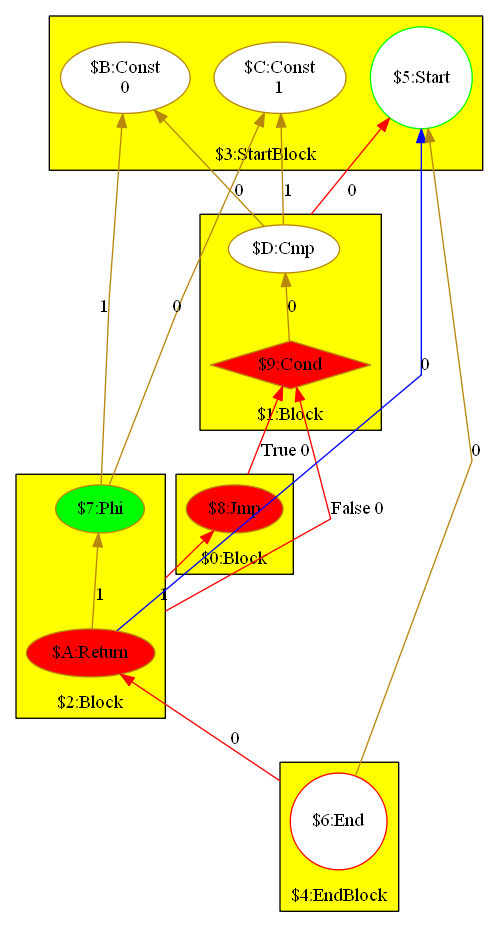
\includegraphics[width=0.5\linewidth]{fig/showgraph2}
\end{center}

Available programs are \texttt{dot}, \texttt{neato}, \texttt{fdp}, \texttt{sfdp}, \texttt{twopi}, \texttt{circo}. 
They are used to transform the graph dumped into a \texttt{dot}-file to a \texttt{png}-file that is then opened with the image viewer of the system.
The executables must be available in the search path of the system (so you have to install graphviz and have to add the \texttt{bin} folder to the path for this to work).

The temporary file(s) will be deleted when the application \emph{Filename} is terminated, in case \GrShell\ is still running at this time.
If the \texttt{keep} parameter was specified, the file(s) will be kept instead.

\begin{rail}
  'dump' 'graph' Filename
\end{rail}\ixkeyw{dump}\ixkeyw{graph}
Dumps the current graph in \indexed{VCG} format into the file \emph{Filename}.\\

\pagebreak

The following commands control the style of the VCG output.
This affects \texttt{dump graph}, \texttt{show graph}, and \texttt{enable debug}.
\begin{rail}
  'dump' 'set' 'node' (() | 'only') NodeType DumpNodeContinuation;
DumpNodeContinuation:
 (('color' | 'textcolor' | 'bordercolor') Color | 'shape' Text | 'labels' ('on' | 'off' | Text)) ;
\end{rail}\ixkeyw{dump}\ixkeyw{set}\ixkeyw{node}\ixkeyw{only}\ixkeyw{color}\ixkeyw{textcolor}\ixkeyw{bordercolor}\ixkeyw{shape}\ixkeyw{labels}\ixkeyw{on}\ixkeyw{off}\ixnterm{DumpNodeContinuation}
Sets the \indexed{color}, text color, border color, the shape or the label of the nodes of type \emph{NodeType} and all of its subtypes.
The keyword \texttt{only} excludes the subtypes. 
The following shapes are supported: \texttt{box}, \texttt{triangle}, \texttt{circle}, \texttt{ellipse}, \texttt{rhomb}, \texttt{hexagon}, \texttt{trapeze}, \texttt{uptrapeze}, \texttt{lparallelogram}, \texttt{rparallelogram}.
Those are shape names of \yComp\ (for a VCG definition see~\cite{vcg}).
The following colors are supported: \texttt{Black}, \texttt{Blue}, \texttt{Green}, \texttt{Cyan}, \texttt{Red}, \texttt{Purple}, \texttt{Brown}, \texttt{Grey}, \texttt{LightGrey}, \texttt{LightBlue}, \texttt{LightGreen}, \texttt{LightCyan}, \texttt{LightRed}, \texttt{LightPurple}, \texttt{Yel\-low} (default), \texttt{White}, \texttt{DarkBlue}, \texttt{DarkRed}, \texttt{Dark\-Green}, \texttt{DarkYellow}, \texttt{DarkMagenta}, \texttt{DarkCyan}, \texttt{Gold}, \texttt{Lilac}, \texttt{Turquoise}, \texttt{Aquamarine}, \texttt{Khaki}, \texttt{Pink}, \texttt{Orange}, \texttt{Orchid}, \texttt{LightYellow}, \texttt{YellowGreen}.
These are the same color identifiers as in \indexed{VCG}/\yComp\ files (for a VCG definition see~\cite{vcg}).

The default labeling is set to \texttt{on} with \texttt{Name:Type}, it can be overwritten by a specified label string (e.g. a source code line originating a node in a program graph) or switched off.

\begin{rail}
  'dump' 'set' 'edge' (() | 'only') EdgeType DumpEdgeContinuation;
DumpEdgeContinuation:
  (('color' | 'textcolor') Color | 'linestyle' (Text) | 'thickness' (Number) | 'labels' ('on' | 'off' | Text));
\end{rail}\ixkeyw{dump}\ixkeyw{set}\ixkeyw{edge}\ixkeyw{only}\ixkeyw{color}\ixkeyw{textcolor}\ixkeyw{labels}\ixkeyw{on}\ixkeyw{off}\ixkeyw{linestyle}\ixkeyw{thickness}\ixnterm{DumpEdgeContinuation}
Sets the color, text color, the linestyle, the thickness of the line, or the label of the edges of type \emph{EdgeType} and all of its subtypes.
The keyword \texttt{only} excludes the subtypes. 
The available colors are given above with the \texttt{dump set node} specification.
The default labeling is set to \texttt{on} with \texttt{Name:Type}, it can be overwritten by a specified label string or switched off.
The following linestyles are supported: \texttt{continuous} (default), \texttt{dotted}, \texttt{dashed}.
The following thicknesses are supported: \texttt{1} (default), \texttt{2}, \texttt{3}, \texttt{4}, \texttt{5}.

\begin{rail}
  'dump' 'add' (('node' ('only')? NodeType)|('edge' ('only')? EdgeType)) 'exclude' ;
\end{rail}\ixkeyw{dump}\ixkeyw{add}\ixkeyw{node}\ixkeyw{edge}\ixkeyw{only}\ixkeyw{exclude}
Excludes nodes/edges of type \emph{NodeType}/\emph{EdgeType} and all of its subtypes from output, for a node it also excludes its incident edges.
The keyword \texttt{only} excludes the subtypes from exlusion, i.e.\ subtypes of \emph{NodeType}/\emph{EdgeType} are dumped.

\begin{rail}
  'dump' 'add' 'node' ('only')? NodeType 'group' (GroupConstraints)? ;
GroupConstraints:
  'by' ('hidden')? GroupMode (IncAdjTypeConstraints)? ;
IncAdjTypeConstraints:
  ('only')? EdgeType ('with' ('only')? NodeType)? ;
\end{rail}\ixkeyw{dump}\ixkeyw{add}\ixkeyw{node}\ixkeyw{only}\ixkeyw{group}\ixkeyw{by}\ixkeyw{hidden}\ixkeyw{with}\ixnterm{GroupConstraints}\ixnterm{IncAdjTypeConstraints}
Declares \emph{NodeType} and subtypes of \emph{NodeType} as \indexed{group node}\indexmainsee{hierarchic}{group node} type.
All the differently typed nodes that point to a node of type \emph{NodeType}
(i.e.\ there is a directed edge between such nodes) will be grouped and visibly enclosed by the \emph{NodeType}-node (leading to the rendering of a nested graph).
\texttt{GroupMode} is one of \texttt{no},\texttt{incoming},\texttt{outgoing},\texttt{any}; \texttt{hidden} causes hiding of the edges by which grouping happens.
The \texttt{EdgeType} constrains the type of the edges which cause grouping, the \texttt{with} clause additionally constrains the type of the adjacent node;
\texttt{only} excludes subtypes.

\begin{warning}
Only apply group commands on a graph if they indeed lead to a containment tree of groups.
If the group commands would lead to a directed acyclic or even cyclic containment graph, the results are undefined.
You may get duplicate edges (and nodes); the implementation is free to choose indeterministically between the possible nestings -- it may even grow an arm and stab you in your back.
(A conflict resolution heuristic used is to give the earlier executed \texttt{add group} command priority.
But this mechanism is incomplete -- you'd better refine your groups or change the model in that case.
Using a model separating edges denoting direct containment from cross-linking edges by type is normally the better design, even disregarding visual node nesting.)
\end{warning}

The following example shows \emph{metropolis} ungrouped and grouped:
\begin{center}
  \fbox{\includegraphics[width=0.45\linewidth]{fig/group2-1}}  \hfill \fbox{\includegraphics[width=0.45\linewidth]{fig/group2-2}}\\
  {\small right side: dumped with \texttt{dump add node metropolis group}}
\end{center}

\begin{rail}
  'dump' 'add' (() | 'only') ('node' NodeType | 'edge' EdgeType) \\ ('infotag' | 'shortinfotag') AttributeName
\end{rail}\ixkeyw{dump}\ixkeyw{add}\ixkeyw{only}\ixkeyw{node}\ixkeyw{edge}\ixkeyw{infotag}\ixkeyw{shortinfotag}
Declares the \indexed{attribute} \emph{AttributeName} to be an ``\indexed{info tag}'' or ``\indexed{short info tag}''.
Info tags are displayed like additional node/edge \indexed{label}s, in format \texttt{Name=Value}, or \texttt{Value} only for short info tags.
The keyword \texttt{only} excludes the subtypes of \emph{NodeType} resp.\ \emph{EdgeType}.

\pagebreak

In the following example \emph{river} and \emph{jam} are info tags:
\begin{center}
  \fbox{\includegraphics[width=0.5\linewidth]{fig/infotag}}
\end{center}

\begin{rail}
  'dump' 'add' 'graph' 'exclude';
  'dump' 'set' 'graph' 'exclude' 'option' ContextDepth;  
\end{rail}\ixkeyw{dump}\ixkeyw{add}\ixkeyw{graph}\ixkeyw{exclude}\ixkeyw{option}
The dump graph exclude commands allow to suppress the display of the graph during debugging.
Instead, only the match of the current rule is shown, plus some context up to a certain depth, plus the parent nodes according to the nesting commands.
The default depth is 1, i.e. the match plus its direct neighbours are displayed (plus the nesting nodes); you may set it to 0 or a higher value.
These commands allow you to still use the debugger if the graph as such is too large to be layed out (or laying it out takes too long to be convenient).

\begin{rail}
  'dump' 'reset'
\end{rail}\ixkeyw{dump}\ixkeyw{reset}
Resets all style options (\texttt{dump set}\dots) and (\texttt{dump add}\dots) to their default values.


\begin{note}\label{note:visual}
Small graphs allow for fast visual understanding, but with an increasing number of nodes and edges they quickly loose this property.
The group commands are of outstanding importance to maintain readability with increasing graph sizes
(e.g. for program graphs it allows to lump together expressions of a method inside the method node and attributes of a class inside the class node).
Additional helpers in keeping the graph readable are:
the capability to exclude elements from dumping (the less hay in the stack the easier to find the needle),
the different colors and shapes to quickly find the elements of interest,
as well as the labels/infotags/shortinfotags to display the most important information directly.
Choose the layout algorithm and the options delivering the best results for your needs, organic and hierarchic or compiler graph
(an extension of hierarchic with automatic edge cutting -- marking cut edges by fat dots, showing the edge only on mouse over and allowing to jump to the other end on a mouse click)
should be tried first.
\end{note}

The following example consisting of Figures~\ref{figprogramgraph1} and \ref{figprogramgraph2} shows several of the layout options employed to considerably increase the readability of a program graph (as given in \texttt{examples/JavaProgramGraphs-GraBaTs08}), with:
\begin{itemize}
	\item nesting to show containment
	\item color coding to distinguish different classes of elements (yellow for classes, magenta for methods, cyan for variables, and green for expressions and statements)
	\item the typical rendering of the \texttt{Hierarchic} layout (its advanced version \texttt{Compilergraph} to be more exact)
\end{itemize}

\begin{figure}[htbp]
  \centering
  \includegraphics[width=0.99\textwidth]{fig/screen-overview}
  \caption{Overview of the initial program graph }
  \label{figprogramgraph1}
\end{figure}

\begin{figure}[htbp]
  \centering
  \includegraphics[width=0.99\textwidth]{fig/screen-detail}
  \caption{Some details of the ``Node'' class of the initial program graph}
  \label{figprogramgraph2}
\end{figure}


\pagebreak


You see the \texttt{exclude} option applied in Figures~\ref{figimdb} and \ref{figimdb2}, stemming from the \GrG{} solution \cite{MovieDatabase} of the TTC14 Movie Database case \cite{MovieDatabaseCase} (you find it under \texttt{examples/MovieDatabase-TTC2014}) .
There, a rule \texttt{couplesWithRating} (whose pattern consists of a \texttt{c:Couple} referencing its actors \texttt{pn1:Person} and \texttt{pn2:Person}) is used in order to fetch the couples of actors who performed together in a movie, for one the couples whose common movies have the highest rating, and for the other the couples with the highest number of common movies. 
The match with the highest rating or highest number is obtained by ordering with an auto-generated filter (cf. \ref{sub:filters}) alongside an appropriately filled \texttt{def} variable, and throwing away the results below with an auto-supplied filter.

\begin{figure}[htbp]
  \centering
  \includegraphics[width=\linewidth]{fig/IMDB}
  \caption{\texttt{couplesWithRating}, order by \texttt{avgRating}, 10,000 movies file}
  \label{figimdb}
\end{figure}

The first screenshot depicted in Figure~\ref{figimdb} was taken on Windows 10 during processing of the 10,000 movies file from IMDB (98,388 nodes, 124,638 edges). 
It is displayed with layout \texttt{Circular} and shows the match of the couple with the highest rating. 

The second screenshot depicted in Figure~\ref{figimdb2} was taken on openSUSE LINUX 13.2 during processing of the generated N=50,000 example (1,000,000 nodes, 1,600,000 edges). 
It is displayed with layout \texttt{Organic} and shows the match of the couple with the highest number of common movies.

The graphs as such are beyond the capabilities of the graph viewer (several thousand graph elements work well, up to a few ten thousand ones), without the \texttt{exclude} we'd be blind, this way we're endowed with partial sight (on the important part, the match plus its context).
Notice the infotags on the \texttt{rating} and \texttt{avgRating} attributes.

\begin{figure}[htbp]
  \centering
  \includegraphics[width=\linewidth]{fig/IMDB2}
  \caption{\texttt{couplesWithRating}, order by \texttt{numMovies}, generated with N=50,000}
  \label{figimdb2}
\end{figure}


\pagebreak


%%%%%%%%%%%%%%%%%%%%%%%%%%%%%%%%%%%%%%%%%%%%%%%%%%%%%%%%%%%%%%%%%%%%%%%%%%%%%%%%%%%%%%%%%%%%%%%%
\section{yComp Usage}

\yComp\indexmain{yComp}\cite{ycomp} (a graph viewer application originally targeting compiler construction, based on the yFiles library) is the default graph viewer of GrGen, and -- when started as a server process -- can be controlled by the debugger via a TCP/IP connection.

The available layouts of \yComp{} are: \texttt{Random}, \texttt{Hierarchic}, \texttt{Organic}, \texttt{Orthogonal}, \texttt{Circular}, \texttt{Tree}, \texttt{Diagonal}, \texttt{Incremental Hierarchic}, \texttt{Compilergraph}, see \ref{sec:debuggercommands} for more.

Besides the things already mentioned in \ref{tools:ycomp}, we want to give the following hints:
\begin{itemize}
	\item when started on a dump, you must press the rightmost play button to start layout
	\item play with the layout options offered in the \texttt{Layout} menu until you find a good visualization, configure it then in the GrShell; don't forget to press the play button to apply the changes
	\item you can pane by pressing and holding the middle mouse button while moving the mouse
	\item you can zoom with the mouse wheel at the position of the cursor
	\item hovering over graph elements displays the attributes
	\item you can select graph elements with the left mouse button and delete them with \texttt{del} to gain a better overview
	\item by activating edit mode with the 3rd rightmost button in the toolbar you can move nodes around, which allows you to fix a bad layout (rather seldomly needed)
	\item the context menu opened by pressing the right mouse button over a graph element allows you to explore the adjacent nodes in non-edit-mode, or delete the element in edit mode
	\item you can search with \texttt{Ctrl-f} or \texttt{/} for the persistent name or an attribute value (or by clicking into the left search field), the matching elements get highlighted
\end{itemize}

%%%%%%%%%%%%%%%%%%%%%%%%%%%%%%%%%%%%%%%%%%%%%%%%%%%%%%%%%%%%%%%%%%%%%%%%%%%%%%%%%%%%%%%%%%%%%%%%
\section{MSAGL Usage}

MSAGL\indexmain{MSAGL}\cite{MSAGL}, an abbreviation of Microsoft Automatic Graph Layout, is a .NET library and tool for graph layout and viewing.
MSAGL is not a standalone application, in contrast to yComp, but a library that is linked into \GrG\ (and used at API level).
Technically, the debugger using MSAGL as graph viewer can be embedded into your own .NET program by utilizing the \texttt{graph\-Viewer\-And\-Sequence\-Debugger.dll} and the \texttt{graph\-Viewer\-And\-Sequence\-Debugger\-Windows\-Forms.dll} of \GrG\ (i.e. you can use it on API level, like MSAGL).
Legally, this is possible because MSAGL comes with the very permissive \indexed{MIT license}\cite{MITLicense}, in contrast to the \yComp{} license purchased by IPD Goos from yWorks that restricts its use to academic purposes, and esp. does not allow you to ship it with a release of your own software.
\GrG\ itself is licensed as LGPL, so you can ship it with your own (even commercial) program - the functionality of the MSAGL based graph viewer is limited compared to what \yComp{} offers, though.

The available layouts of MSAGL are: \texttt{SugiyamaScheme}, \texttt{MDS}, \texttt{Ranking}, \texttt{IcrementalLayout}, see \ref{sec:debuggercommands} for more.

In order to use it from \GrShell{}, you have to employ the \texttt{debug with} command.
\begin{rail}
  'debug' 'with' ( 'yComp' | 'MSAGL' )
\end{rail}\ixkeyw{debug}\ixkeyw{with}
Switches the graphical part of the debugger (the graph viewer) in between yComp and MSAGL (with \yComp{} being the default).
If MSAGL is used, the debugger is displayed in a WindowsForms\cite{WinForms} console like control instead of a stdout console.

The program graph from \texttt{examples/JavaProgramGraphs-GraBaTs08} looks like depicted in Figures~\ref{figprogramgraph3} and Figures~\ref{figprogramgraph4} (compared to the \yComp{}-rendering in Figures~\ref{figprogramgraph1} and \ref{figprogramgraph2}).

\begin{figure}[phtb]
  \centering
  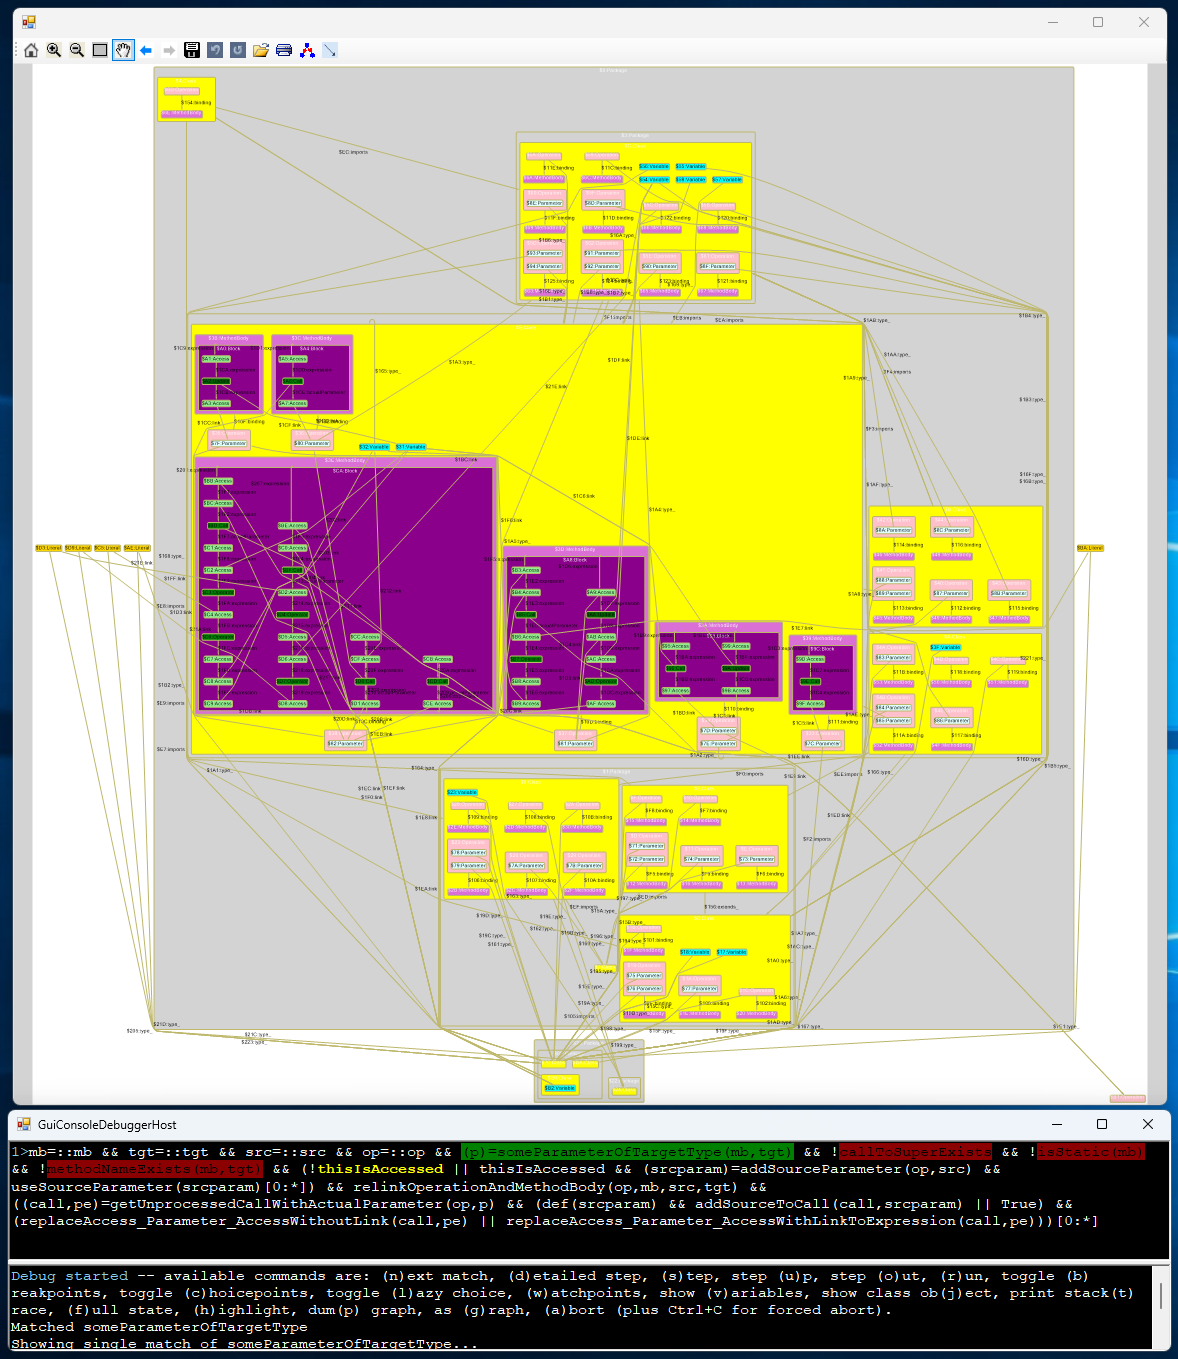
\includegraphics[width=0.99\textwidth]{fig/screen-msagl-overview}
  \caption{The initial program graph rendered with MSAGL and layout SugiyamaScheme, utilized by a debugger with two console panes}
  \label{figprogramgraph3}
\end{figure}

\begin{figure}[phtb]
  \centering
  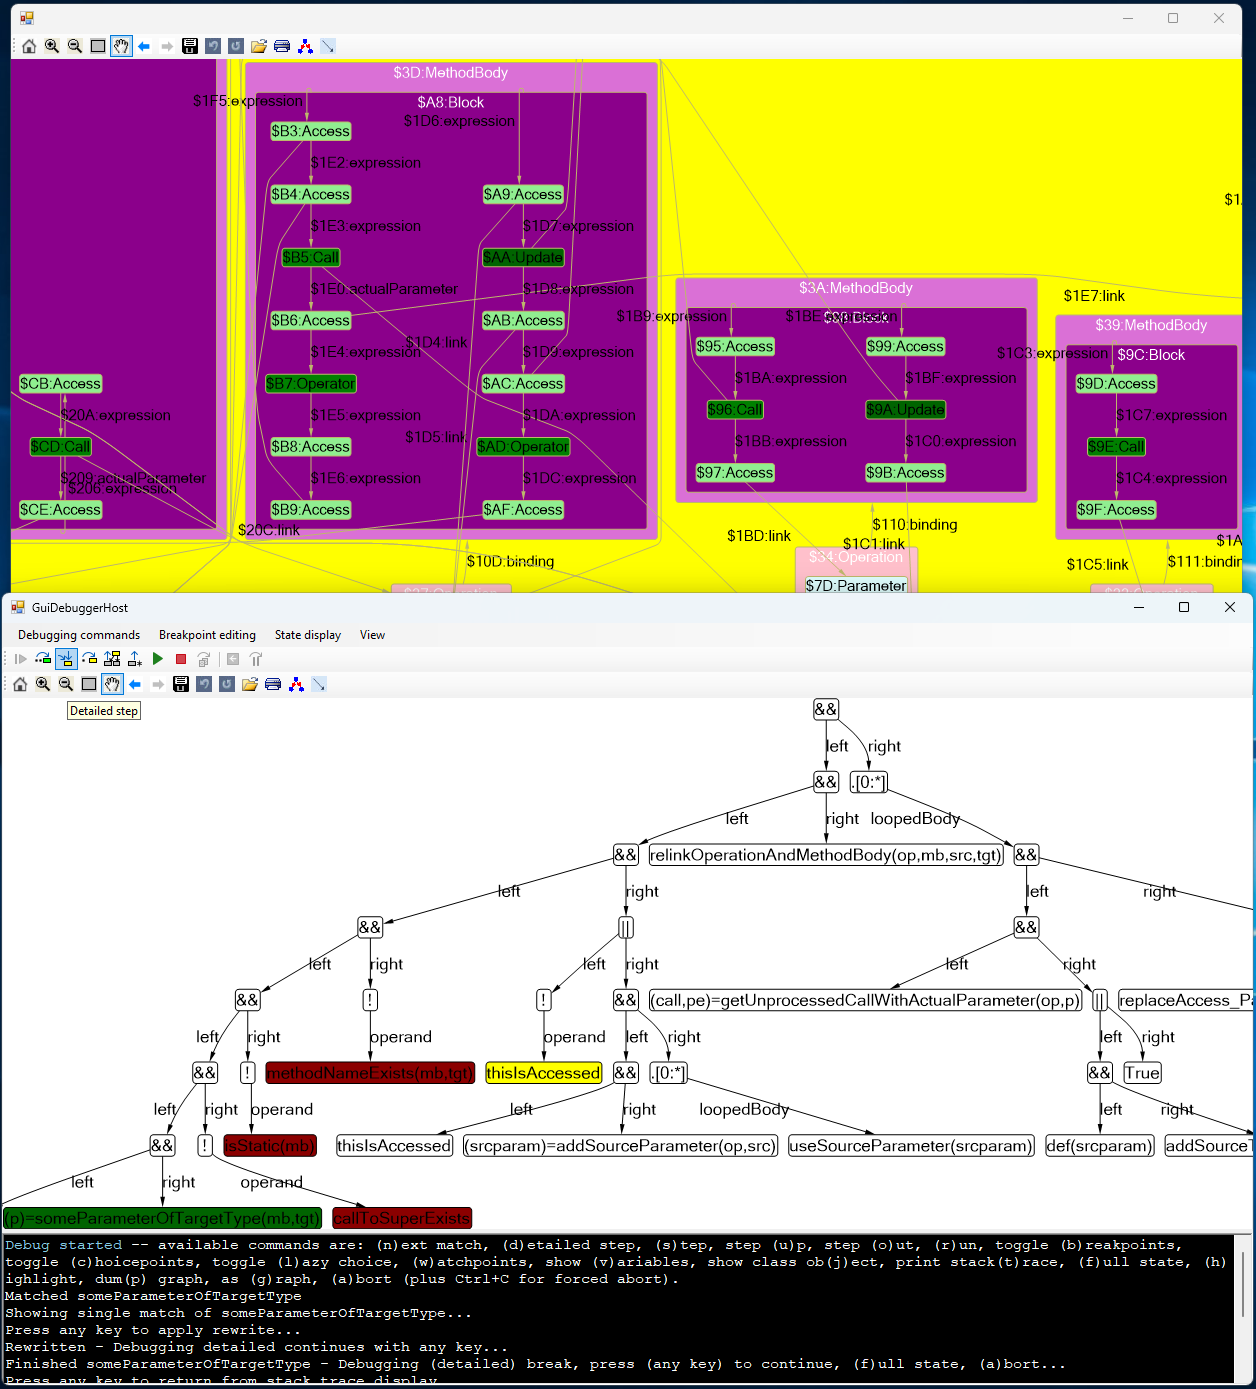
\includegraphics[width=0.80\textwidth]{fig/screen-msagl-detail}
  \caption{Some details of the ``Node'' class of the initial program graph}
  \label{figprogramgraph4}
\end{figure}

The WindowsForms based debugger that uses MSAGL as graph viewer supplies a two pane mode, it is enabled by default in this case (when \yComp{} is used, only the single \GrShell{}-console is employed, irrespective of this setting), you may disable it (or enable it again) with the configuration option:
\begin{rail}
  'debug' 'set' 'option' 'twopane' ( 'true' | 'false' )
\end{rail}\ixkeyw{debug}\ixkeyw{set}\ixkeyw{option}\ixkeyw{twopane}
In two pane mode of the debugger, two consoles are employed, one for data rendering and one for user dialog.
The data rendering console only displays the current work object at a time (typically the sequence that gets debugged, in its current state), instead of the complete output history, which still holds for the user dialog console, esp. in order to allow you to inspect the subrule traces log.

You may find out whether two pane mode is enabled with the following command:
\begin{rail}
  'debug' 'get' 'options'
\end{rail}\ixkeyw{debug}\ixkeyw{get}\ixkeyw{options}
Lists the available debug options.


%%%%%%%%%%%%%%%%%%%%%%%%%%%%%%%%%%%%%%%%%%%%%%%%%%%%%%%%%%%%%%%%%%%%%%%%%%%%%%%%%%%%%%%%%%%%%%%%
\section{Debugging Related Commands}\label{sec:debuggercommands}

\begin{rail}
  'debug' ( 'enable' | 'disable' )
\end{rail}\ixkeyw{debug}\ixkeyw{enable}\ixkeyw{disable}
Enables and disables the \indexed{debug mode}.
The debug mode shows the current working graph in a \yComp{} or MSAGL window.
All changes to the working graph are tracked by the graph viewer immediately.

\begin{rail}
  'debug' 'set' 'layout' ( (Text)? | 'option' Name String ) ;
\end{rail}\ixkeyw{debug}\ixkeyw{set}\ixkeyw{layout}\ixkeyw{option}
Sets the default graph \indexed{layout algorithm} to \emph{Text}.
If \emph{Text} is omitted, a list of the available layout algorithms is displayed.
The \texttt{option} version allows you to specify layout options by name value pairs.
The available layout options can be listed by the succeeding command.

The following layout algorithms are supported by \yComp{}: \texttt{Random}, \texttt{Hierarchic}, \texttt{Organic}, \texttt{Orthogonal}, \texttt{Circular}, \texttt{Tree}, \texttt{Diagonal}, \texttt{Incremental Hierarchic}, \texttt{Compilergraph}.
For technical graphs \texttt{Hierarchic} works normally best; \texttt{Compilergraph} is a version of \texttt{Hierarchic} cutting some edges, it may be of interest if \texttt{Hierarchic} contains too many crossing edges.
\texttt{Organic} is the other general purpose layout algorithm available to be tried out early; the other layout algorithms are rather special, but this should not deter you from using them if they fit to your task ;).

The following layout algorithms are supported by MSAGL: \texttt{SugiyamaScheme}, \texttt{MDS}, \texttt{Ranking}, \texttt{IcrementalLayout}.
We recommend to use \texttt{SugiyamaScheme} in place of \texttt{Hierarchic}, and \texttt{MDS} in place of \texttt{Organic}.

\begin{rail}
  'debug' 'get' 'layout' 'options';
\end{rail}\ixkeyw{debug}\ixkeyw{get}\ixkeyw{layout}\ixkeyw{options}
Prints a list of the available layout options of the currently active layout algorithm.

\begin{rail}
  'debug' 'get' 'layout';
\end{rail}\ixkeyw{debug}\ixkeyw{get}\ixkeyw{layout}
Prints the currently set layout.

\begin{rail}
  'debug' 'layout';
\end{rail}\ixkeyw{debug}\ixkeyw{layout}
Forces re-layout of the graph shown in yComp (same as pressing the play button within yComp).

\begin{rail}
  'debug' 'set' 'node' 'mode' Text DumpNodeContinuation ;
\end{rail}\ixkeyw{debug}\ixkeyw{set}\ixkeyw{mode}
\begin{rail}
  'debug' 'set' 'edge' 'mode' Text DumpEdgeContinuation ;
\end{rail}\ixkeyw{debug}\ixkeyw{set}\ixkeyw{mode}
Configures the display of the visual debug states for the nodes/edges.
The following modes are supported: \texttt{matched}, \texttt{created}, \texttt{deleted}, \texttt{retyped}.
Change this if you e.g. want the matched elements to be marked more visibly, or added/deleted elements to be colored green/red (instead of red/grey).

\begin{rail}
  'debug' 'set' 'match' 'mode' ('pre' | 'post') ('enable' | 'disable');
\end{rail}\ixkeyw{debug}\ixkeyw{set}\ixkeyw{mode}
Configures the behavior of the debugger regarding the display of found matches.
When pre-match debugging is enabled, the matches of a (multi) rule execution before filtering/selection are displayed in detail steps, the default is disable. 
When post-match debugging is enabled, the matches of rules in embedded execs are displayed in detail steps
(with post-match disabled, only the match(es) of the very rule followed by the rewrite of the rule), the default is enable.

\begin{rail}
  GraphRewriteSequence: 'debug' ('exec'|'xgrs') SimpleRewriteSequence ;
\end{rail}\ixkeyw{debug}\ixkeyw{exec}\ixkeyw{xgrs}\indexmain{graph rewrite sequence}\indexmainsee{GRS}{graph rewrite sequence}\ixnterm{GraphRewriteSequence}
This executes the graph rewrite sequence \emph{SimpleRewriteSequence} in the debugger\indexmain{debugger}.
The semantics is the same as for \texttt{exec SimpleRewriteSequence} already introduced in Chapter~\ref{chapgrshell}, but you can trace the execution step-by-step.

\begin{rail}
  GraphRewriteSequenceExpression: 'debug' ('eval') SequenceExpression ;
\end{rail}\ixkeyw{debug}\ixkeyw{eval}\indexmain{graph rewrite sequence expression}
This executes the graph rewrite sequence expression \emph{SequenceExpression} in the debugger\indexmain{debugger}.
The semantics is the same as for \texttt{eval SequenceExpression} already introduced in Chapter~\ref{chapgrshell}, but you can watch the matches highlighted in the graph (one (multi) rule query after the other).

\pagebreak

%%%%%%%%%%%%%%%%%%%%%%%%%%%%%%%%%%%%%%%%%%%%%%%%%%%%%%%%%%%%%%%%%%%%%%%%%%%%%%%%%%%%%%%%%%%%%%%%
\section{Using the Debugger}

Put abstractly, a graph rewrite sequence is executed step-by-step, one rule application after the other, yielding a series of execution states.
Each step has a current point of execution in the sequence, referencing the rule that is to be or gets applied.
The debugging process can be described as a reduced view on such a series of execution states,
consisting of a series of debugging situations, which are a subset of your choice of the execution states reached in time.
In each debugging situation or step, the execution state or a a subset of it is rendered.

This means concretely, that the debugger\indexmain{debugger} -- which is a part of the \GrShell~--
prints the debugged sequence with the currently focused/active rule highlighted yellow.
What will be shown from executing this rule depends on the chosen debug command,
and on the fact whether the focused rule matches or not.
An active rule which is already known to match is highlighted green.
The rules that matched the last time during sequence execution are shown on dark green background,
the rules that failed the last time during sequence execution are shown on dark red background;
at the begin of a new loop iteration the highlighting state of the rules contained in the loop is reset.

During execution, \yComp\footnote{Make sure, that the path to your \texttt{\indexed{yComp.jar}} package is set correctly in the \texttt{ycomp} shell script within \GrG's \texttt{/bin} directory.}\indexmain{yComp}/MSAGL
displays the current graph at each single step, and on request highlights a rule application, marking the matches in the graph, and showing the changes to the graph stemming from that rule application.

%\pagebreak %manual break to get two pages with halfway broken layout instead of one with deeply broken

Besides deciding on what is shown from the application of the current rule, you also determine with the debug commands where to continue debugging, i.e. the rule focused next;
but of course this depends strongly on the following flow of execution, esp. the fact whether the execution of the currently active rule succeeds/fails, and the execution state in general.

%maybe todo: explain s(k)ip mode/skipping

With the \texttt{s} debug command (step) you execute the current rewrite rule (trying to match it, applying the rewrite on success) and then continue with the next rule in the sequence.

With the \texttt{n} debug command (next) you fast-forward to the next rule \emph{that matches}, and apply it when pressed again.

With the \texttt{r} debug command (run) you continue execution until sequence termination or until a breakpoint is hit.

With the \texttt{d} debug command (detailed step) you execute the current rewrite rule, if it matches highlighting its match and then the changes in the graph, and then continue with the next rule in the sequence.
In case the rule contains embedded sequences, these are also executed in detail mode (unless switched off with \texttt{set match mode post disable}).
In case pre match debugging is toggled on (\texttt{set match mode pre enable}), all the matches found are displayed in a pre-step, before filtering (which may remove matches) and selection (of e.g. the active rule in a some from set construct).

All the available debug commands are given in Table~\ref{tabdebug}.
An example debugging run is shown in the following example \ref{ex:debug}.

\pagebreak

In addition to the commands for actively stepping or skipping through the sequence execution,
there are breakpoints and choicepoints available (toggled with the \texttt{b} and \texttt{c} commands),
which become active if execution reaches them, even if a user command would skip over them in the debugging process.

The \indexed{break point}s halt execution, focus the reached sequence, and cause the debugger to wait for further commands
(e.g. \texttt{d} to inspect the rule execution en detail versus \texttt{s} for just applying it).

The \indexed{choice point}s halt execution, focus the reached sequence in magenta, and ask for some user input;
after the input was received, execution continues according to the command previously issued.

Both break points and choice points are denoted by the \texttt{\%} modifier.
The \texttt{\%} modifier acts as a break point if it is given before: a rule, an all bracketed rule, a variable predicate, or the constants \texttt{true}/\texttt{false}.
The \texttt{\%} modifier acts as a choice point if it is appended to the \texttt{\$} randomize modifier, switching a random decision into a user decision.
The dollar randomize modifier can be applied to the binary operators, the random match selector of all bracketed rules, the random-all-of operators and the one-of-set braces.
The idea behind this is: you need some randomization for \indexed{simulation} purpose --- then use the randomize modifier \texttt{\$}.
You want to force a certain decision, overriding the random decision, in order to try out another execution path while debugging the simulation --- then modify the randomize modifier with the user (choice) modifier \texttt{\%}.

The initial breakpoint and choicepoint assignment is given with the \texttt{\%} characters in the sequences after the \texttt{debug exec} commands in the \texttt{.grs} file.
The breakpoint and choicepoint commands of the debugger allow to toggle them at runtime, overriding the initial assignment (notationally yielding a sequence with added or removed \texttt{\%} characters).
The user input commands \texttt{\$\%(type)} define choice points which cannot be switched off.

Moreover, there are commands available that allow to print the variables at a given situation, or the sequence call stack, or a full state dump of the call stack and the variables.

Further commands allow to dump the current graph, or highlight elements in the graph, defined by being contained in a (possibly container valued) variable, or being marked according to a visited flag.

In addition, you may crawl the network of objects or transient objects, starting at a variable or object defined by its unique id.

%\pagebreak

\begin{table}[htbp]
  \begin{tabularx}{\linewidth}{|lX|}
\hline
  \texttt{s}(tep) & Execute the current rewrite rule (matching it, and rewriting in case it matched; the resulting graph is shown).\\
  \texttt{d}(etailed step) & Execute the current rewrite rule in a three-step procedure: 
    matching - highlighting the found match, rewriting - highlighting the changing elements, 
    and completion - carrying out the rewrite, showing the resulting graph, then executing subrules from embedded sequences (\texttt{exec}), step by step. \\
  (step) \texttt{o}(ut) & Continue execution until the end of the current loop. 
    If execution is not in a loop at this moment, but in a sequence called, the called sequence will be executed until its end.
    If neither is the case, the complete sequence will be executed.\\
  (step) \texttt{u}(p) & Ascend one level up within the \indexed{Kantorowitsch tree} of the current rewrite sequence (i.e. rule; see Example~\ref{ex:debug}; at the moment the command is pretty useless because only the serialized form is displayed).\\
  \texttt{r}(un) & Continue execution (until the end or a breakpoint).\\
  \texttt{a}(bort) & Cancel execution immediately.\\
  \texttt{n}(ext) & Go to the next rewrite rule that matches, make it current.\\
\hline
  (toggle) \texttt{b}(reakpoint) & Toggle a breakpoint at one of the breakpointable locations.\\
  (toggle) \texttt{c}(choicepoint) & Toggle a choicepoint at one of the choicepointable locations.\\
  (edit) \texttt{w}(atchpoints) & Allows to edit data breakpoints or the behaviour of programmed debug messages.\\
\hline
  \texttt{v}(ariables) & Prints the global variables and the local variables of the sequence currently executed, which is the topmost sequence of the sequence call stack.
    Plus the allocated visited flags. To be more precise: all local variables which were defined (and have not fallen out of scope again) up to the sequence position focussed.\\
  \texttt{t}(race) & Prints the stack trace of the current sequence call stack.
     The stack trace includes the body of each sequence called at its execution state.\\
  \texttt{f}(ull dump) & Prints the stack trace including the local variables of each stack frame plus the global variables.\\
  (dum)\texttt{p} (graph)\label{dumpgraph} & Dumps the current graph as a \texttt{.vcg} file and shows it in yComp. 
    This can be used as a workaround to check the real state in case transaction/backtracking rollback is used on a graph with node nesting, which may lead to a buggy display.
    In addition, an \texttt{undo.log} is written with the undo commands of the open transactions for \emph{change reversal}, which would be applied on rollback.\\
  (as)-\texttt{g}(raph) & Asks for the value of the externally defined type that is to be shown in the debugger in graph form 
    (you must implement an extension handler able to return an \texttt{INamedGraph} on request for this to work, see \ref{sub:apiextemitparse}). 
    Alternatively, you may specify a graph value, which is then displayed directly.\\
  \texttt{h}(ighlight)\label{highlight} & Highlights the elements in the graph that are marked with the visited flag given, or are contained in the variable given (which might be a simple scalar variable containing one graph element, or a container variable potentially containing multiple ones). 
     Multiple variables or visited flags may be given separated by commas.\\
  (show ob)\texttt{j}(ect)\label{showobject} & Shows the object defined by its unique id or a transient object by a just generated id. You may give a variable name as root element to start crawling at (in order to obtain a transient object id).\\
\hline
  \end{tabularx}
  \caption{\GrShell\ debug commands}
  \label{tabdebug}
\end{table}
%\begin{figure}[htbp]
%  \centering
%  \includegraphics[width=0.25\linewidth]{fig/debug1}\includegraphics[width=0.4\linewidth]{fig/debug2}\includegraphics[width=0.4\linewidth]{fig/debug3}
%  \caption{Delayed step rule application.}
%  \label{figdebug}
%\end{figure}

%\pagebreak

\begin{figure}[htbp]
\begin{example}\label{ex:debug}
We demonstrate the debug commands by executing a slightly adjusted script for generating the Koch snowflake from \GrG's examples (see also Section~\ref{fractals}).
The graph rewrite sequence is
\begin{grshell}
debug exec (makeFlake1* & (beautify & doNothing)* & makeFlake2* & beautify*)[1]
\end{grshell}
\yComp\ will be opened with an initial graph:
\begin{center}
  \includegraphics[width=0.3\linewidth]{fig/debug0tra}
\end{center}
We type \texttt{d}(etailed step) to apply \texttt{makeFlake1} in detail mode with a matching, rewriting, and completion substep, resulting in the following graphs:
\begin{center}
  \parbox{0.2\linewidth}{\includegraphics[width=\linewidth]{fig/debug1tra}}\parbox{0.375\linewidth}{\includegraphics[width=\linewidth]{fig/debug2tra}}\parbox{0.375\linewidth}{\includegraphics[width=\linewidth]{fig/debug3tra}}
\end{center}
The following table shows the active rule reached after having entered the preceeding debug command, for a series of debug commands:
\begin{center}
  \begin{tabular}{|l|l|} \hline
    \textbf{Command} & \textbf{Active rule} \\ \hline
    \texttt{s} & \texttt{makeFlake1} \\
    \texttt{o} & \texttt{beautify} \\
    \texttt{s} & \texttt{doNothing} \\
    \texttt{s} & \texttt{beautify} \\
    \texttt{u} & \texttt{beautify} \\
    \texttt{o} & \texttt{makeFlake2} \\
    \texttt{r} & --- \\ \hline
  \end{tabular}
\end{center}
\end{example}
\end{figure}

%\subsection{yComp}
%url; yFiles; java app, socket communication with shell debugger
%Find; goto node/edge; b�bbels;
%relayout; zoom: mousewheel; pane by holding middle mouse
%supported formats; vcg format
%ref to visualization commands, again: hierarchy
%copy some of the stuff from ycomp help?

\pagebreak

%%%%%%%%%%%%%%%%%%%%%%%%%%%%%%%%%%%%%%%%%%%%%%%%%%%%%%%%%%%%%%%%%%%%%%%%%%%%%%%%%%%%%%%%%%%%%%%%
\section{Subrule Debugging and Programmed Halts}\label{secdebuggersubrule}

The basic granularity of debugging in \GrG{} is the single rule (with its pattern matched and its rewrite carried out) executed from an interpreted sequence.
But with embedded execs there are further sequences and actions available outside direct control of and visibility in the debugger.
At least some debugging aide is available for them, at least the actions called from the embedded sequences are shown in the debugger -- in case detailed mode is used.
But the local execution state of imperative code which may be used for tasks where pattern matching is not beneficial is completely invisible to the debugger.
Only the effects on the graph become visible.

There is a remedy available for this situation in the form of code-embedded debugging commands, realized by calls to procedures from the built-in package \texttt{Debug}.
With them you can punch holes into the covering blanket that allow you to peek at what's going on under the covers.
The debugging commands are used for one to directly display information, but for the other for handling a stack of debug messages, intended for representing the current state of the call nesting of the executing code.

The available commands are:
\begin{description}
\item[\texttt{Debug::add(message(,object)*)}] to be called when a subrule computation or an interesting piece of code is entered.
The message is added to the debug messages stack of the debugger.
Besides the mandatory \texttt{message:string}, an arbitrary number of other parameters may be given (of arbitrary type).
\item[\texttt{Debug::rem(message(,object)*)}] to be called when a subrule computation or an interesting piece of code is exited.
The topmost entry message on the messages stack is removed.
It is checked that the message of the topmost added entry is identical to the message of current removal -- you must always call \texttt{add} and \texttt{rem} in pairs!
The \texttt{emit} messages on the way to the topmost \texttt{add} are removed. 
Besides the mandatory \texttt{message:string}, an arbitrary number of other parameters may be given (of arbitrary type).
\item[\texttt{Debug::emit(message(,object)*)}] to be called when some interesting points in the code are passed.
The message is added to the debug messages stack of the debugger.
Besides the mandatory \texttt{message:string}, an arbitrary number of other parameters may be given (of arbitrary type).
\item[\texttt{Debug::halt(message(,object)*)}] to be called when some point in the code is reached that is so interesting that you want the execution to break in the debugger. 
If called, the debugger halts execution, displays the messages stack in its current state, and prints out the halt message with its parameters.
Besides the mandatory \texttt{message:string}, an arbitrary number of other parameters may be given (of arbitrary type).
\item[\texttt{Debug::highlight(message(,object,string)*)}] to be called when some point in the code is reached that is so interesting that you want the execution to break in the debugger, 
in order to highlight some nodes or edges graphically in the debugger, in the same way they are highlighted when an action is matched.
If called, the debugger halts execution, displays the messages stack in its current state, and displays the nodes and edges passed with the additional parameters highlighted in the graph.
The additional parameters must be given in pairs, first the entity to display, then the string that entry will be annotated with in the debugger.
The entity to display may be a node or edge, which is then directly highlighted,
or a storage containing nodes or edges, all contained nodes/edges will then be highlighted,
or a visited flag (integer number), all graph elements that are visited according to that flag are then highlighted.
Besides, as first mandatory parameter, the \texttt{message:string} must be given.
\end{description}

Some \texttt{add} and \texttt{rem} are automatically inserted by \GrG{} for you.
For one for embedded execs, a debug message is sent when an embedded exec is entered or exited, with a message starting with the name of the containing rule.
For the other for procedures and compiled sequence definitions, a debug message is sent when a procedure or defined sequence is entered or exited, with a message being equal to the name of the procedure or defined sequence.

%%%%%%%%%%%%%%%%%%%%%%%%%%%%%%%%%%%%%%%%%%%%%%%%%%%%%%%%%%%%%%%%%%%%%%%%%%%%%%%%%%%%%%%%%%%%%%%%
\section{Watchpoint configuration}

The behaviour of the debugger upon receiving certain events can be defined with configuration rules aka watchpoints.
They are contained in a list, ordered by time of insertion.
When a subrule debugging event (a debug message as introduced in the previous section), or a graph change event, or an action match event occurs,
the list of watchpoints is visited one entry after the other, and one configuration rule checked for a match after the other.
When a configuration rule or watchpoint matches, its decision is applied.
The decision may be to break execution and display the current execution state, or to continue execution, which is of interest for events that normally break execution but should be better ignored.

Besides defining the configuration rules of the watchpoints beforehand with shell commands, you can edit them interactively with the edit \texttt{w}atchpoint command inside the debugger. 

\subsection*{Subrule messages}

\begin{rail}
  'debug' 'on' ('add'|'rem'|'emit') MessageFilter 'break';
  'debug' 'on' ('halt'|'highlight') MessageFilter 'continue';
	MessageFilter: ('equals' | 'startsWith' | 'endsWith' | 'contains') '(' StringConstant ')';
\end{rail}\ixkeyw{debug}\ixkeyw{on}\ixkeyw{add}\ixkeyw{rem}\ixkeyw{emit}\ixkeyw{halt}\ixkeyw{highlight}\ixkeyw{break}\ixkeyw{continue}\ixnterm{MessageFilter}\ixkeyw{equals}\ixkeyw{startsWith}\ixkeyw{endsWith}\ixkeyw{contains}

When the string specified matches the message of the debug event according to the message filter given,
execution is interrupted by the debugger in case of a \texttt{Debug::add}, or \texttt{Debug::rem}, or \texttt{Debug::emit}, and the execution state of the code (esp. specified by those commands) is presented in the debugger.
Normally, those events are handled silently.
When a match happens for a \texttt{Debug::halt} or \texttt{Debug::highlight}, execution is continued without interruption, while normally those messages break execution in the debugger.

\subsection*{Action match event}

\begin{rail}
  'debug' 'on' 'match' RuleName ('break'|'continue') ('if' SequenceExpression)?;
\end{rail}\ixkeyw{debug}\ixkeyw{on}\ixkeyw{match}\ixkeyw{break}\ixkeyw{continue}\ixkeyw{if}

When the action specified was matched, execution is halted in the debugger in case of a \texttt{break}.
This is of interest for rules executed from execs, as normal breakpoints don't apply to them, this way we can set a breakpoint on a rule irrespective from where it is called 
(allowing us to just \texttt{r}un a sequence until an action match of interest happens).
In case of a \texttt{continue}, execution is forced to continue.
This is of interest for detail mode debugging that normally breaks on each matched rule.
It allows us to skip over uninteresting rules in execs without the need to acknowledge them.

The sequence expression finally allows us to decide conditionally.
It is evaluated when its corresponding configuration rule is evaluated because its match event occurred, if it returns true the configuration rule matches, otherwise it does not match.
The \texttt{this} entity is overloaded in the sequence expression (normally it denotes the graph).
It gives access to the match found, you can access the entities of the match in dot-Notation (e.g. \texttt{this.node1}).
The configuration rule is evaluated for all matches in case of an all-bracketed match, if one returns true, the decision is carried out.

\subsection*{Graph change events}

\begin{rail}
  'debug' 'on' ('new'|'delete'|'retype'|'set' 'attributes') TypeNameSpec 'break' \\ ('if' SequenceExpression)?;
	TypeNameSpec: ('only')? Type | railat '(' Name')';
\end{rail}\ixkeyw{debug}\ixkeyw{on}\ixkeyw{new}\ixkeyw{delete}\ixkeyw{retype}\ixkeyw{set}\ixkeyw{attributes}\ixkeyw{break}\ixnterm{TypeNameSpec}\ixkeyw{only}\ixkeyw{if}

When the graph change specified occurred (its corresponding event was fired), execution is halted in the debugger.
The supported graph changes are graph element creation, deletion, retyping, and attribute assignment.
The \emph{TypeNameSpec} constrains this by type or by name.
The first form matches only when the element is of the specified type, in case of \texttt{only} only if it is of exactly that type and not a subtype.
The second form matches only when the element is of the specified name, given as string constant 
(rules of that kind are typically created interactively, but due to the persistence of persistent names and the execution of GrGen being as deterministic as possible in between single runs, even static rules make sense -- even more so if you assign the names on your own).

The sequence expression finally allows us to decide conditionally.
It is evaluated when its corresponding configuration rule is evaluated because its graph change event occurred, if it returns true the configuration rule matches, otherwise it does not match.
The \texttt{this} entity is overloaded in the sequence expression (normally it denotes the graph).
It gives access to the node or edge that was just created, or is getting deleted, or is getting retyped, or was assigned to.
So here we find support for conditional data breakpoints.


%%%%%%%%%%%%%%%%%%%%%%%%%%%%%%%%%%%%%%%%%%%%%%%%%%%%%%%%%%%%%%%%%%%%%%%%%%%%%%%%%%%%%%%%%%%%%%%%
\section{Debugging related functionality}

Other commands that are of use for debugging were already introduced in the shell chapter:\\
\verb#show var <Variable># to print the content of a variable and \\
\verb#show <GraphElement>.<AttributeName># to print the content of an attribute.\\
But pressing the \texttt{v} key in the shell debugger is more convenient in the former case, as is searching with \texttt{Ctrl-f} or \texttt{/} in yComp for the persistent name or an attribute value, hovering over the then highlighted graph element, in the latter case.

The commands \verb#record# and \verb#replay# are of interest when you want to follow different paths during a transformation, they allow you to save the graph states before choosing in between the different paths, and to restore them later on (and to inspect the sequence of changes leading to a graph state).

Another development aide comes in the form of validity checking code that gets emitted when the \texttt{-debug} option is supplied to \texttt{grgen.exe} (cf. \ref{grgenoptions}), the usage of that option can be also configured in the shell (cf. \ref{sec:compilerconfigshell}).
The validity checking code detects with runtime checks situations in which: 
\begin{enumerate}
	\item a rule is called with a null argument (unless it was specified that null parameters are allowed, in that case the missing element is searched for in the graph)
	\item a rule is called with a graph element as parameter that is not contained in the graph anymore
	\item a match is about to be rewritten with a matched graph element that is not contained in the graph anymore
\end{enumerate}

The first case typically happens when an initialization of a variable is missing, or when a graph global variable gets auto-nulled, because the graph element was deleted. 

The second case typically happens when a node or edge was removed from the graph but is still held in a local variable or a storage. 

The third case typically happens during an all-bracketed rule application that matched a graph element multiple times, and now wants to retype the graph element, after having executed a previous rewrite, that deleted that particular graph element (an all-bracketed rule application rewrites one match after the other). 
The situation may be rather obvious, when the graph element was bound to the same pattern element in different matches, it may be also quite difficult to grasp, because the graph element was bound to different pattern elements in different matches.
The check may fail without uncovering a real issue, because the already deleted element is not to be modified with the rewrite of the current match (or only to be deleted again, deletion after deletion is not causing a crash).

Regarding the third case, note that an edge not contained in the graph anymore is not reported as invalid in case its source or target nodes are not contained in the graph anymore (this safes you from spurious error reports, at the price of potentially missing a situation where this is not anticipated).
By annotating a node/edge with a \texttt{validityCheck=false}, cf. Section \ref{annotations}, you can disable the contained-in-graph check for that graph element.
By using the same annotation on a rule (cf. Table \ref{tabannotations}), you can disable this validity check for all graph elements that were matched during the execution of the rule.


\chapter{Indices and Performance Optimization}\label{cha:performance} \indexmain{performance}\indexmain{optimization}

The most important point to understand when optimizing for speed is that the expensive task is the search carried out during pattern matching. The effort of rewriting (the dominant theme in graph rewriting literature) is negligible.

Searching is carried out with a backtracking algorithm following a search plan in a fixed order, 
binding one pattern element after another to a graph element, checking if it fits to the already bound parts.
If it does fit search continues trying to bind the next pattern element (or succeeds building the match object from all the elements bound if the last check succeeds), if it does not fit search continues with the next graph element; if all graph element candidates for the currently focused pattern element are exhausted, search backtracks to the previous decision point and continues there with the next element.

Typically, first a graph element is determined with a lookup operation reaching into the graph, binding the element to a graph element of the required type (the less elements of that type exists, the better) -- then neighbouring elements are traversed following the graph structure (the less neighbouring elements exists, the better), until a match of the entire pattern is found.


%%%%%%%%%%%%%%%%%%%%%%%%%%%%%%%%%%%%%%%%%%%%%%%%%%%%%%%%%%%%%%%%%%%%%%%%%%%%%%%%%%%%%%%%%%%%%%%%
\section{Search Plans}

A search plan for the pattern in figure \ref{perf:figpatterntosearch} is:\\
\texttt{lkp(v1:A); out(v1,e1:a); tgt(e1,v2:B); out(v2,e3:b); tgt(e3,v3:C); out(v3,e2:a)}\\
The search operation \texttt{lkp} denotes a node (or edge) lookup in the graph, \texttt{out} follows the outgoing edges of the given source node and \texttt{in} follows the incoming edges of the given target node, while \texttt{src} fetches the source from the given edge and \texttt{tgt} fetches the target from the given edge.

For some graphs the search plan might work well, but for the graph given in figure \ref{perf:figgraphtosearchin} it is a bad search plan.
Why so can be seen in the search order sketched in figure \ref{perf:figbadsearch}.
Due to the multiple outgoing edges of \texttt{v1} of which only one leads to a match it has to backtrack several times.

This schedule in contrast is a a good one:\\
\texttt{lkp(v3:C); out(v3,e2:a); tgt(e2,v2:B); out(v2,e3:b); in(v2,e1:a); src(e1,v1:A)}\\
corresponding to the search order depicted in figure \ref{perf:figgoodsearch}.

It is crucial for achieving high performance to prevent following graph structures splitting into breadth as given in this example, and especially to avoid lookups on elements which are available in high quantities.

\begin{figure}[p]
  \centering
  \includegraphics[width=0.7\textwidth]{fig/Pattern}
  \caption{Pattern to search}
  \label{perf:figpatterntosearch}
\end{figure}

\begin{figure}[p]
  \centering
  
\includegraphics[width=0.7\textwidth]{fig/Graph}
  \caption{Host graph to search in}
  \label{perf:figgraphtosearchin}
\end{figure}

\pagebreak

\begin{figure}[p]
  \centering
  \includegraphics[width=0.7\textwidth]{fig/GraphBad}
  \caption{Bad search order}
  \label{perf:figbadsearch}
\end{figure}

\begin{figure}[p]
  \centering
  \includegraphics[width=0.7\textwidth]{fig/GraphGood}
  \caption{Good search order}
  \label{perf:figgoodsearch}
\end{figure}


%%%%%%%%%%%%%%%%%%%%%%%%%%%%%%%%%%%%%%%%%%%%%%%%%%%%%%%%%%%%%%%%%%%%%%%%%%%%%%%%%%%%%%%%%%%%%%%%
\section{Find, Don't Search}
It is better to find elements with certain characteristics straight ahead without search,
utilizing a data structure that allows to tell the elements that follow the characteristic apart from the ones that do not,
than to search for them, traversing each and every node or edge in the graph, subjecting it to a test for the characteristic.

Welcome to indices as known from database parlance.
In \GrG{} the following types of indices are supported:
\begin{enumerate}
	\item Type indices
	\item Neighbourhood indices
	\item Attribute indices
	\item Incidence count indices
	\item Name index
	\item Uniqueness index
\end{enumerate}

%-----------------------------------------------------------------------------
\subsection{Type Indices}
All the nodes or edges in \GrG{} of a certain type are contained in a list that can be accessed in $O(1)$ and iterated in $O(k)$ with $k$ being the number of elements in that list (the nodes or edges of same type), in contrast to $n$, being the number of nodes or edges in the graph.
The first node or edge in a pattern is typically bound by iterating such a type list.
In case the pattern is disconnected, a lookup is needed per connected component.
In case multiple types have very few members, the search planner may decide to use several lookups even in case of a connected pattern.
(This can be especially the case for reflexive marker edges pointing to the current point of processing/focus of attention in the graph.)

%-----------------------------------------------------------------------------
\subsection{Neighbourhood Indices}
All the edges outgoing from a node are contained in a list that can be accessed in $O(1)$ and iterated in $O(k)$ with $k$ being the number of elements in that list (the outgoing edges), in contrast to $n$, being the number of edges in the graph.
All the edges incoming to a node are contained in a list that can be accessed in $O(1)$ and iterated in $O(k)$ with $k$ being the number of elements in that list (the incoming edges).
So following neighbouring elements, crawling alongside the structure is very cheap in \GrG{ } -- and possible in both directions, following the edges as well as in their opposite direction.

It is cheap in graph databases, too, but absolutely not in relational databases.
To follow a relation, there you have to join two complete tables, building the cartesian product of two tables (materializing only the rows where they agree) -- you must inspect all edges in the graph to find the neighbours.
Typically you optimize this with a database index that allows to find the elements of the second table matching your focused element of the first table in $O(log(n))$ -- but for large $n$ or for complex queries this global product is way less efficient than direct local access to exactly the neighbouring elements.
(Furthermore, a table join is conceptually and notationally much heavier than an edge in a graph pattern).

In case of undirected edges, or arbitrary directed edges in the pattern, both directions are searched,
both lists -- the outgoing list as well as the incoming list -- are crawled.

\pagebreak %improve layout

%-----------------------------------------------------------------------------
\subsection{The Costs}\label{sec:performancememory} 
The type and neighbourhood indices are built into each and every \GrG{} graph, wired into a system of ringlists (cf. \ref{sec:generatedcode}).
They are implicitly used by \GrG{}, pattern matching is carried out alongside them, in an order decided upon by the search planner. 

You always benefit from them during matching (most if you are using statistics-based search planning), but you must always pay their price:
The memory consumption of a \GrG{} node without attributes is 36 bytes using a 32bit CLR (5 pointers a 4 bytes, a 4 bytes flags field/bitvector, a 4 bytes unique id field, plus 8 bytes .NET object overhead), it is 64 bytes for a 64bit CLR (5 pointers a 8 bytes, a 4bytes flags field, a 4 bytes unique id field, plus 16 bytes .NET object overhead).
The memory consumption of a \GrG{} edge without attributes is 52 bytes using a 32bit CLR (9 pointers a 4 bytes, a 4 bytes flags field/bitvector, a 4 bytes unique id field, plus 8 bytes .NET object overhead), it is 96 bytes for a 64bit CLR (9 pointers a 8 bytes, a 4 bytes flags field, a 4 bytes unique id field, plus 16 bytes .NET object overhead).
Attributes are cheap, they only increase this by the .NET-memory-footprint of their underlying objects.

The runtime price of maintaining those indices during graph manipulation is low, adding a graph element is done in $O(1)$, removing a graph element is done in $O(1)$, too. 
Furthermore, those indices allow to optimize loops by letting the pattern matching of the next iteration start where the previous iteration left of (search state space stepping -- a further built-in contribution to the motto "Find, Don't Search")).

We consider this the best you can get for the task of efficient pattern matching and rewriting on typed, attributed multigraphs, with multiple inheritance and attributes on nodes as well as edge types -- those indices are simply worth their price in the general case.
You can only improve on this by exploiting the specifics of a less general graph model, a less general processing strategy supporting less change operations optimally out-of-the box, or by restricting yourself to less general and non-automatic pattern matching.
E.g. by using only single-linked ringlists for the types and incident elements, we could reduce memory consumption considerably and thus increase query performance, but deletion and retyping would require to iterate the full list to get to the predecessor to link it to the new successor, so rewriting would not be $O(1)$ anymore.
Or by always entering the graph at some elsewhere stored root nodes we could save the type ringlists (that give us the modularity of the rules).
Or by using less general edges/edges that appear only with a statically fixed association cardinality, we could reduce them to mere pointers stored in the nodes (not supporting attributes, not allowing to wire nodes at runtime flexibly with an arbitrary number of edges).

\GrG\ was built for general-purpose graph pattern matching and rewriting on a general model, to perform well on \emph{any} task, with \emph{minimum programming effort} for the user; regarding this it is implemented in a way we consider optimal and not improvable.
If you are willing to invest extra programming and understanding effort to exploit the specifics of your task at hand, you \emph{can} manually code a higher-performance solution, by stripping away features from the model you don't need.
Saving on the memory needed for the generality and programming productivity is what gives our competitor FUJABA a lead performance-wise for tasks where a simpler graph model is sufficient and the user is willing to invest more development time into (and no iterative search-replace-operations are carried out, search state space stepping wins then).

\pagebreak %improve layout

%-----------------------------------------------------------------------------
\subsection{Consequences For Optimization}

\subsubsection*{Use types!}
Fine grain types cause a fast lookup of the first pattern element(s), or more exactly: they cause a small list of candidate elements for the first pattern element to be tried.
And they cause quicker pruning of search branches because of early failing type checks.
Using fine-grain types is easy in GrGen, as multiple inheritance on node and edge types (cf. \ref{nodeandedgetypes}) is supported.
Besides, the more fine grain the graph is typed, the better are the statistics, allowing \GrG{ } to find better search plans (see more for this below).

\subsubsection*{Prune early}
Attribute conditions are evaluated as soon as all needed graph elements are matched (saving us from enumerating futile match extensions).
But the unit of scheduling are the full attribute condition expressions. 
If an expression can be separated into different parts that depend on less pattern elements than the entire expression (such a separation is trivial for boolean expressions joined by logical conjunctions), split it into those parts.
The parts are then checked earlier in the search process.
You could even introduce checks that are logically not needed because a later check removes all incorrect matches anyway, just to achieve better performance, which is the case if the checks allow to prune some branches from the search space earlier.
This holds as long as the checks are cheap, if they are expensive you could do the opposite and introduce artificial dependencies to all pattern elements instead, to ensure the attribute condition is evaluated as late as possible.

%\pagebreak

\subsubsection*{Prefer directed edges}
Non-directed edges in the pattern are searched in both directions, considerably increasing the search space.
Use non-directed edges only if they you really needed them.
For some problems this is the case, you then simply have to pay the price of the increased effort for the symmetry.
But some problems where undirected edges are more natural can be easily encoded with directed ones -- in case of performance problems, refactor and optimize them to employ only directed edges, imposing an arbitrary but deterministic direction on the edges.
Besides, the vstructure statistics are more discriminating in case of directed edges, leading to better search planning results; in case of undirected ones the information from both directions is coalesced.

%\pagebreak

\subsubsection*{Beware of Disconnected Patterns}
Disconnected patterns cause a combinatorial explosion of the matches, because the overall number of matches equals the cartesian product of the partial matches of the disconnected parts. 

This is inevitable and a price that must be simply paid if this is really needed.
But it is normally not needed, and, most importantly, is not specified accidentally, as a disconnected pattern in a single flat pattern is typically immediately visible.
But take care of nested patterns or subpatterns.
You might overlook that nested patterns and subpatterns are matched strictly one after the other and especially after their containing pattern.
You cannot ignore block borders and subpattern calls, they disconnect otherwise connected components.
Esp. take care of not disconnecting patterns when factoring out a common part into a subpattern to improve the code.
But due to inlining, things look better than what was said until now.

\begin{example}
Take a look at pattern nesting, when the pattern is disconnected, you run into issues due to combinatorial explosion.
This holds for sure for alternative and iterated patterns.

So you must take care of pattern cardinality ...
\begin{grgen}
test bad {
  n1:Node; n2:Node; // builds cartesian product of all nodes in the graph (O(n*n))
  multiple {
    n1 --> n2; // then filters it down to the connected nodes
  }
}
\end{grgen}
... and alternatives ...
\begin{grgen}
test bad {
  n1:Node; n2:Node; // builds cartesian product of all nodes in the graph (O(n*n))
  alternative {
    single {
      n1 --> n2; // then filters it down to the connected nodes
    }
  }
}
\end{grgen}
\end{example}

\begin{example}
Take a look at pattern nesting, when the pattern is disconnected, you run into issues due to combinatorial explosion.
This may hold for independent and subpatterns -- but inlining is of help here.

The edge from the independent in the example is typically inlined into the pattern removing the issue...
\begin{grgen}
test bad {
  n1:Node; n2:Node; // builds cartesian product of all nodes in the graph (O(n*n))
  independent {
    n1 --> n2; // then filters it down to the connected nodes
  }
}
\end{grgen}
... as is the subpattern body inlined into the pattern, removing the performance issue.
\begin{grgen}
test bad {
  n1:Node; n2:Node; // builds cartesian product of all nodes in the graph (O(n*n))
  :P(n1,n2);
}
pattern P(n1:Node, n2:Node) {
  n1 --> n2; // then filters it down to the connected nodes
}
\end{grgen}
Take a look at the output of the \texttt{explain} command to check whether inlining occurred.
\end{example}

The need to take nested pattern borders and subpattern calls into account is due to the recursive descent matching with a multi-pushdown machine as described in Section \ref{matchingflow} and Section \ref{pushdownmachine}.

Subpatterns are matched top-down, from the input parameters on.
If the input arguments are disconnected in the pattern containing the subpattern, the containing pattern enumerates the cross product of the matches of the disconnected parts, which is only later on filtered for the ones which are connected.
This will likely wreak havoc on search performance.
Even if you don't search for all matches, if you only compute a single overall match --- the calling pattern must enumerate a lot of combinations of its parts (worsened by the fact that those are typically found often because of their simplicity), until the nested pattern finally is able to connect one of the disconnected pairs fed into it.
It might be more efficient to just search from a start parameter towards a connected end location, and yield the found one out (cf. \ref{sec:localvarorderedevalyield}); or to search from a start parameter on all connected end locations, collecting the found ones in a result set -- and then to check the ones found alongside connectedness in a second step.

Nested patterns are also matched top-down, from the input parameters on. 
But parameter passing is implicit here, the elements from the containing pattern that are referenced in the nested pattern are passed in automatically as arguments.
This holds especially for the \texttt{alternative} and \texttt{iterated} constructs, which are matched with the pushdown machine (cf. \ref{pushdownmachine}), too, but also for the \texttt{negative} and \texttt{independent} constructs, which are matched with nested local code embedded into the matcher code of their containing pattern.

But don't shy away from using subpatterns or independents too early, \indexed{inlining} is of help here!

The elements from an independent that are linking a disconnected pattern are typically inlined into their using pattern.
The elements from a subpattern are often inlined into their using pattern, causing the pattern to get connected (again), 
but also removing the pushdown machine overhead.
But you must take into account that the \emph{inlining} implemented in GrGen is limited to depth one.
If a pattern is disconnected over two or more levels of subpattern usage (which might happen statically with one subpattern using another subpattern, and will for sure dynamically on a subpattern recursion path), it will hit performance.
You may have a look at the output of the \texttt{explain} command (cf. \ref{custom}) to see if the subpatterns are disconnected.
This is typically indicated by multiple lookups in the containing pattern, 
for fetching the disconnected starting points,
which are then handed down with preset parameters to the nested or subpatterns,
and only get connected there,
with search commands following their outgoing or incoming edges.

%-----------------------------------------------------------------------------
\subsection{Search Planning On Request}
Search planning at runtime is only carried out on request!
You must analyze the graph and then re-generate the matchers manually,
with \texttt{custom graph analyze} and \texttt{custom actions gen\_searchplans} issued on the command line, 
or with calls of the \texttt{Custom} methods of the \texttt{IGraph} and the \texttt{IActions} objects.
Unless you do so, the static search plan is kept in place.

You can display the search plan currently employed with the \texttt{custom actions explain <actionname>} command,
in order to inspect how the pattern elements are matched.
Issue it before search planning to show the statically generated search plan, issue it afterwards to show the dynamically re-generated search plan.
See subsection \ref{custom} for more on this.

The initial static search plan typically starts with a lookup of an arbitrary edge, and then arbitrarily follows the pattern graph structure.
Interestingly, in many cases this still works quite well because of the quick pruning by the type checks in a well-typed graph.
In addition, often the rules match from some parameter nodes onwards, which are typically well-suited starting points for searching.

Beware: the \texttt{analyze} command is costly.
It helps in improving the matching performance, but requires execution time on its own.
Don't use it freely.

It is costly because it has to visit all the nodes and edges in the graph,
in order to gather statistical data about the amount of breadth-splitting per node and edge-types. 
For each $(NodeType, EdgeType, NodeType\ast)$-triple (for all node and edge types), it counts for each start node of $NodeType$ the number of edges of $EdgeType$, which are leading to an end node of $NodeType\ast$.
Given that information, search planning is able compute a search plan that avoids to follow structures splitting into breadth (V-structures) that occur often in the host graph.
Given the information about the element counts per type (which is directly available from the host graph), 
search planning is able to compute a search plan that avoids lookups on populated types.

Such a dynamically generated search plan typically leads to minimum matching durations, but not always -- sometimes you may fare better by manually assigning priorities to the pattern elements, thus influencing the search order in the initial static search plan (high-prio elements are matched first).

Again: Use types!
The more fine grain a graph is typed, the better are the statistics regarding the breadth-splitting and the number of elements of a certain type, and the better are then in consequence the search plans in their ability of evading breadth-splitting structures and avoiding lookups of often occurring types.

%-----------------------------------------------------------------------------
\subsection{Attribute Indices}
In addition to the built-in type and neighbourhood indices, you may declare attribute indices.
An attribute index allows to do a lookup based on an attribute value, or a range of attribute values.
This stands in contrast to the default behaviour of carrying out a lookup on a type, visiting all $n$ elements of the type, filtering them down to the elements of interest (within range) with an attribute condition.
If this means you have to inspect a lot of values while searching only for a few ones, you should use an attribute index and benefit from its massively improved selectivity for the lookup.
It requires only $O(log(n))$ to search for the first element, and $O(k)$ for the $k$ elements within the bounds specified.
It is implemented with a balanced binary search tree (an AA-tree\cite{Andersson93balancedsearch} to be exact) that requires three pointers plus one 4 byte integer per element contained in the index (two pointers to the left and right tree nodes, and one to the graph element as value), which is really cheap.
But it must be maintained on graph changes, which is less cheap.
On each and every graph element insertion and removal, but esp. attribute assignment, the index has to be updated, which is an $O(log(n))$ operation.
That's only logarithmic, but clearly worse than the default $O(1)$ behaviour of \GrG{}, so if you do a lot of graph manipulations and only few lookups based on it, an index may in fact degrade performance.

\subsubsection*{Declaration in the model}
In contrast to type and neighbourhood indices that are always available (they define the core of a \GrG{}-graph) and implicitly used (when matching a specified pattern), all other indices have to be worked with explicitly.

An attribute index must be declared in the model.

\begin{rail}
  AttributeIndexDecl: 'index' IndexName lbrace Type '.' AttributeName rbrace;
\end{rail}\ixnterm{AttributeIndexDecl}

Following the \texttt{index} keyword, a name for the index is specified; in the body of the index, the type and name of the attribute to be indexed are given.

\subsubsection*{Usage in the rules}\label{sub:indexusage}

In the pattern part you may ask for an element to get bound to an element from an index;
this is syntactically specified by giving the index access enclosed in left and right braces after the element declaration.
If the type of the element retrieved from the index is not compatible to the type of the pattern element specified,
or if the index is empty, matching fails.
The elements from the index are successively bound to the pattern element, then the rest of the pattern is bound and checked, until the requested number of matches is found.

\begin{rail}
  IndexAccess:
    lbrace IndexName '==' Expression rbrace |
		lbrace ('ascending'|'descending') '(' (IndexBound (',' IndexBound)?)? ')' rbrace;
	IndexBound: IndexName ('<'|'<='|'>'|'>=') Expression;
\end{rail}\ixnterm{IndexAccess}

The pattern element may be bound to the elements from the index with an attribute value equal to a specified value,
or to the elements from the index in ascending or descending order.
In case of ordered access, you may specify no bound, this is typically only of interest when a single match is requested, the one with the highest or lowest attribute value (satisfying the other constraints of the pattern), or you may specify a lower bound, or an upper bound, or a lower \emph{and} an upper bound.

\begin{rail}
  IndexAccessLoopStatement:
    ForIndexAccessHeader lbrace (Statement*) rbrace;
  ForIndexAccessHeader:
    'for' '(' Var ':' GraphElementType 'in' IndexAccess ')';
  IndexAccessLoopSequence:
    'for' lbrace Var ':' GraphElementType 'in' IndexAccess ';' RewriteSequence rbrace;
\end{rail}\ixnterm{IndexAccessLoopStatement}\ixnterm{IndexAccessLoopSequence}

The index can be accessed furtheron from the statements of the rule language in the form of a loop.
The \emph{IndexAccess} in the loop header follows the format used in the index access in the pattern.
The iteration variable is bound to the graph element retrieved from the index, and then, for each such element, the body is executed.

Moreover, the index can be iterated over in the sequences.

\begin{example}
The following index \texttt{foo} allows to quickly fetch nodes of type \texttt{N} (or a subtype) based on the value of its attribute \texttt{i}.

\begin{grgen}
node class N {
  i : int;
}
index foo { N.i }
\end{grgen}

Fetching typically occurs in the rules, binding a pattern element based on the constraints specified with the lookup.
The test \texttt{t} only matches if a node is found whose attribute \texttt{i} matches the parameter \texttt{j}.
The rule \texttt{r} ascendingly binds the nodes whose attribute \texttt{i} is greater than or equal $5$ and lower than $13$.
The ascendingly means that the node \texttt{n} with smallest attribute \texttt{i} is matched that satisfies the other constraints of the pattern (if there are no further constraints like in this example, it is the node with smallest attribute satisfying the limits of the index access).

\begin{grgen}
test t(var j:int) {
  n:N{foo==j};	
}

rule r {
  n:N{ascending(foo>=5, foo<13)};

  modify {
  ---
    emit("The value of attribute i is ", n.i, "\n");
  }
}
\end{grgen}

An index may also be queried with a \texttt{for} loop from the statements, accepting the same bounds; 
or with a \texttt{for} loop from the sequences.

\begin{grgen}
rule rd {
  modify {
  ---
    eval {
      for(n:N in {descending(foo<=13)}) {
        emit("The value of attribute i is ", n.i, "\n");
      }
    }
    exec (
      for{n:N in {descending(foo<=13)}; {emit("The value of attribute i is ", n.i, "\n")} }
    );
  }
}
\end{grgen}

\end{example}

%-----------------------------------------------------------------------------
\subsection{Incidence Count Indices}
Attribute indices can be seen as a general-purpose device, that extends the built-in ability of quick lookup by-type and of quick lookup by-neighbourhood with a quick lookup by-attribute, thus giving complete quick-lookup coverage for all foundational elements of the graph model.
Incidence count indices in contrast are more of a special-purpose device for a certain abstraction that can be applied to a graph -- the \emph{count} of incident edges -- and are beneficial only if that abstraction is of importance.
They allow you to quickly look up nodes based on their number of incident edges.
This is especially beneficial for algorithms that work best when they traverse the nodes from the ones with the highest number of incident edges to the ones with the lowest number of incident edges (or the other way round).

The index furtheron allows to fetch the incidence count for a node quickly with just an index lookup, 
but typically no gain can be made from this, as counting the incident edges of a node is commonly cheap (an $O(log(n)$ index lookup versus an $O(k)$ counting enumeration, with $k$ being the number of edges incident to the focused node).

\subsubsection*{Declaration in the model}

An incidence count index must be declared in the model.

\begin{rail}
IncidenceCountIndexDecl: 'index' IndexName lbrace IncidenceFunction rbrace;
CountIncidenceFunction: 
  CountIncidenceFunctionName '(' NodeType ')' |
  CountIncidenceFunctionName '(' NodeType ',' EdgeType ')' |
  CountIncidenceFunctionName '(' NodeType ',' EdgeType ',' NodeType ')'
  ;
\end{rail}\label{IncidenceCountIndexDecl}

Following the \texttt{index} keyword, a name for the index is specified; in the body of the index, the incidence function and its types are given.
The admissible count incidence functions are \texttt{countIncident}, \texttt{countIncoming}, and \texttt{countOutgoing}, with semantics as already introduced in \ref{sub:querybyneighbourhood}.
(The count of the edges complying to the specified incidence function is stored in an index, for all nodes in the graph of the type of the first node in the count incidence function.)

\subsubsection*{Usage in the rules}
An incidence count index can be used in the pattern in exactly the same way as an attribute index, see above \ref{sub:indexusage}.

In addition to the index lookup in the pattern, 
the count may be queried from the rule language expressions (the attributes can be accessed directly for a pattern element, the incidence count would have to be counted in contrast, but this only saves time for heavily connected nodes).

\begin{rail}
  IncidenceCountIndexAccessExpr:
    IndexName '[' Expression ']';
\end{rail}\ixnterm{IncidenceCountIndexAccessExpr}

The index access specified in indexer notation expects a node (of the type as specified with the first node type in the incidence function) as input argument, and returns the incidence count for that node as stored in the index as \texttt{int}.

\begin{example}
The following index \texttt{bar} allows to quickly fetch nodes based on the number of \texttt{outgoing} edges, \texttt{qux} allows to quickly fetch nodes of type \texttt{N} based on the number of \texttt{incoming} edges of type \texttt{E}, stemming from a source node of type \texttt{N}.

\begin{grgen}
node class N {
	i:int = 0;
}
edge class E;
index bar { countOutgoing(Node) }
index qux { countIncoming(N, E, N) }
\end{grgen}

Fetching typically occurs in the rules, binding a pattern element based on the constraints specified with the lookup.
The test \texttt{t} returns the node \texttt{n} in the graph with the maximum number of outgoing edges.
The rule \texttt{r} ascendingly binds the nodes whose number of incoming edges of type \texttt{E} from a node of type \texttt{N} is greater than or equal the value of attribute \texttt{i} of node \texttt{l} matched before (constrained to values below $42$ by the \texttt{if}); it \texttt{emit}s the count of outgoing edges of \texttt{n}, queried from the index \texttt{bar} with array access notation.

\begin{grgen}
test t() {
	n:Node{descending(bar)};
}

rule r() {
  l:N; if{ l.i<42;}
  n:N{ascending(qux>=l.i)};
	
  modify {
  ---
    emit("count outgoing(Node): ", bar[n], "\n");
  }
}
\end{grgen}

\end{example}

%-----------------------------------------------------------------------------
\subsection{Name Index}\label{sec:nameindex}
A named graph is a graph where each element bears a unique name and can be looked up quickly by that name.
So basically it works as a graph with an integrated key-value store from a string to a graph element, and one from a graph element to a string.
It is implemented with two hash maps, one from the names to the elements, and the other from the elements to the names.
Lookup is carried out in $O(1)$ (either way).
Maintaining the index on graph insertions and removals is carried out in $O(1)$, too.
So in contrast to the attribute index and the incidence count index, a name index does not allow multiple elements per indexed property (which is here the name).

\subsubsection*{No declaration needed}
The name index does not need to be declared, it is implemented with the named graph, which is always generated together with its sibling, the non-named graph.
If you are working with the \GrShell, this is the only kind of graph you'll be working with, as the shell always instantiates the named graph (it delivers the \emph{persistent names} you see in the debugger).
At API level you may opt for the non-named graph that is considerably cheaper regarding memory usage -- a named graph requires not much less than about twice the amount of memory of a plain graph (unless heavily attributed).

But please note in that case that the export and import capabilities require uniquely named elements and thus only work with named graphs.
If given a plain graph, the exporters just create a named graph.
A graph is always created as a named graph by the importers.
So non-named graphs are typically only of interest if you don't need to persist them into a serialization format.

\subsubsection*{Usage in the rules}
The name index can be used in the pattern to look up graph elements by their name, with the same syntax as used in the GrShell for accessing elements by their (persistent) name.

\makeatletter
\begin{rail}
  NamedIndexAccessExpr:
    lbrace '@' '(' Expression ')' rbrace;
\end{rail}\ixnterm{NamedIndexAccessExpr}
\makeatother

There is at most one element existing with the name asked for; if no graph element with that name exists, matching fails and backtracks, if an element exists, the pattern element is bound to it, and matching continues.
Please note that the (string-)expression used to compute the name is only allowed to reference at most one other pattern element (not handed in as parameter).

The name index may be further queried from the rule language expressions with 3 functions:
\begin{description}
\item[\texttt{nameof(.)}] returns the name (type string) of the given node or edge (or (sub)graph, a missing argument amounts to the host graph).
\item[\texttt{nodeByName(.)}] returns the node of the given name, or null if no node of that name exists. Optionally, a target node type may be given as second argument, then you receive a node of that type as result, or null if no node of that name \emph{and type} exists.
\item[\texttt{edgeByName(.)}] returns the edge of the given name, or null if no edge of that name exists. Optionally, a target edge type may be given as second argument, then you receive an edge of that type as result, or null if no edge of that name \emph{and type} exists.
\end{description}

The names are normally automatically assigned (computed from a global counter increased with each element, prepended by the dollar symbol -- unless you specify a name with an attribute initialization list, cf.\ref{sec:attribinitrule}), but you may assign a different name to an attribute element.
This can be only done in an \texttt{eval}-block, or a \texttt{procedure}, with a \texttt{nameof}-assignment.

\begin{rail}
  NameofAssignment:
    'nameof' '(' Element ')' '=' Expression;
\end{rail}\ixnterm{NameofAssignment}\ixkeyw{nameof}

When you do so, it is your responsibility to ensure that the name does not already exist, otherwise the assignment will cause a runtime exception.
The same syntax may be used to assign the name of a (sub)graph, a missing element amounts to the host graph.

\begin{example}
The test \texttt{t} succeeds if there is a node of name "foo" existing in the graph, with a reflexive edge of the name defined by input parameter \texttt{s}, and there is a further node of name "bar" existing the graph.

\begin{grgen}
test t(var s:string) {
  n:Node{@("foo")} -e:Edge{@(s)}-> n;
  if{ nodeByName("bar") != null; }
}
\end{grgen}

The rule \texttt{r} \texttt{yield}s the name of the node matched to \texttt{n} out to \texttt{oldname}, and changes the name of the node in the \texttt{modify} part by prepending the name of the host graph. Furthermore, it prints the name of the edge bound to \texttt{e}.

\begin{grgen}
rule r() {
  n:Node -e:Edge->;
---
  def var oldname:string;
  yield { yield oldname = nameof(n); }
		
  modify {
    eval {
      nameof(n) = nameof() + "_" + oldname;
    }
  ---
    emit("The name of the graph element bound to e is ", nameof(e), "\n");
  }
}
\end{grgen}

\end{example}


%-----------------------------------------------------------------------------
\subsection{Uniqueness Index}\label{sec:uniqueness}
Uniqueness can be applied in two parts, the i) uniqueness \emph{constraint}, and ii) the uniqueness \emph{index}.

The uniqueness \emph{constraint} ensures that each element in the graph has a unique id. 
It allows in addition to fetch the unique id from a graph element.
You may see it as a key-value store from graph elements to their ids -- it is a very efficient one, as the unique-id is stored in the graph elements. 

The uniqueness \emph{index} allows in addition to fetch a graph element by its unique id, extending the uniqueness property to an index allowing for quick graph element lookup.
You may see it as a key-value store from the unique ids to their graph elements.
This one is realized with an array of unique ids to graph elements.

So lookup is carried out efficiently in $O(1)$ either way.
Maintaining the uniqueness information is in $O(log(n))$, but much less on average, as the ids of deleted elements have to be stored in a heap (the data structure, not the memory model) for quick reuse of the lowest one upon graph element addition (this way we ensure a maximally packed id range, which keeps the index array and the is-matched-bit-arrays of the parallelized matchers small and packed).

A uniqueness index does not allow multiple elements per indexed property (which is here the unique id), like the name index, and in contrast to the attribute and incidence count indices.

\subsubsection*{Declaration in the model}
The space for the unique id is always reserved in the graph elements, but unique ids are only assigned if you declare an uniqueness constraint.
Or if you declare another index in the model, as indices depend on the unique ids, or if you use parallelize annotations, as the parallelized matchers depend on the unique ids, too.
If you need to fetch graph elements by their unique ids, you must declare an unique index (in addition or instead).

\begin{rail}
  UniqueConstraintDecl: 'node' 'edge' 'unique' ';';
  UniqueIndexDecl: 'index' 'unique' ';';
\end{rail}\ixnterm{UniqueConstraintDecl}\ixnterm{UniqueIndexDecl}


\subsubsection*{Usage in the rules}
The unique index can be used in the pattern to lookup graph elements by their unique id.

\begin{rail}
  UniqueIndexAccessExpr:
    lbrace 'unique' '[' Expression ']' rbrace;
\end{rail}\ixnterm{UniqueIndexAccessExpr}

There is at most one element existing with the unique id asked for; if no graph element with that unique id exists, matching fails and backtracks, if an element exists, the pattern element is bound to it, and matching continues.
Please note that the expression used to compute the unique id is only allowed to reference at most one pattern element (not handed in as parameter).

The unique constraint may be further queried from the rule language expressions with the \texttt{uniqueof} function,
the unique index with the \texttt{nodeByUnique} and \texttt{edgeByUnique} functions:
\begin{description}
\item[\texttt{uniqueof(.)}] returns the unique id (type int) of the given node or edge (or (sub)graph, a missing argument amounts to the host graph).
\item[\texttt{nodeByUnique(.)}] returns the node of the given unique id, or null if no node of that unique id exists. Optionally, a target node type may be given as second argument, then you receive a node of that type as result, or null if no node of that unique id \emph{and type} exists.
\item[\texttt{edgeByUnique(.)}] returns the edge of the given unique id, or null if no edge of that unique id exists. Optionally, a target edge type may be given as second argument, then you receive a edge of that type as result, or null if no edge of that name \emph{and type} exists.
\end{description}

The unique ids are automatically assigned (utilizing an id pool that is enlarged with newly allocated ids when an element is added to the graph but the pool is empty, or reusing an already existing id; when an element is removed from the graph, its id returns to the id pool).
In contrast to the names, you cannot change the id assignment.

\begin{example}

The following model declares a node class \texttt{N}, specifies the uniqueness constraint, and requests the uniqueness index.
 
\begin{grgen}
node class N;
node edge unique;
index unique;
\end{grgen}

The test \texttt{t} succeeds if there is a node of unique id $0$ existing in the graph, with a reflexive edge of the unique id defined by input parameter \texttt{i}, and there is a further node of unique id $42$ existing the graph. It is unlikely you will really use code like that as you cannot assign a unique id.

\begin{grgen}
test t(var i:int) {
  n:N{unique[0]} -e:Edge{unique[i]}-> n;
  if{ nodeByUnique(42) != null; }
}
\end{grgen}

The rule \texttt{r} allows to match \texttt{n} and \texttt{m} to the same graph element \texttt{hom}omorphically, just to forbid it then with the condition requesting that their unique-ids must be different. The point here is that the \texttt{hom} allows the engine to omit the isomorphy check, yielding slightly better performance. By using \verb#<# instead of \verb#!=# we ensure that we get only one match for the automorphic pattern in case of an application with all-bracketing -- the one in which the element with the smaller id is bound to \texttt{n}. Furthermore, the rule prints the unique id of the node bound to \texttt{n}.

\begin{grgen}
rule r() {
  n:N -- m:N;
  hom(n,m);
  if{ uniqueof(n) < uniqueof(m); }
		
  modify {
  ---
    emit("The unique id of the graph element bound to n is ", uniqueof(n), "\n");
  }
}
\end{grgen}

\end{example}


%%%%%%%%%%%%%%%%%%%%%%%%%%%%%%%%%%%%%%%%%%%%%%%%%%%%%%%%%%%%%%%%%%%%%%%%%%%%%%%%%%%%%%%%%%%%%%%%
\section{Location Passing and Memorization}
Often in a transformation, you know the location that needs processing from a previous step.
In this case, return these locations out from the rules, store them in variables of node (or edge) type, and hand them in again via rule arguments to the follow-up rules.
Or call embedded rules, directly handing in elements from the containing rule, saving you the intermediate assignments.

Commonly, this is just the right way of handling this situation, 
as you must continue processing the very spot you just processed with the previous rule(s) to achieve a valid result.
Sometimes you don't need to, but gain higher performance when you do so.
Optimize this way then, use \emph{rooted} pattern matching, with roots defined by previous rules, it's cheaper as it saves you the lookup in the graph.

A different way of parameter passing is adding reflexive edges to the graph to mark the spot of processing.
This is normally working well, too, but the parameter passing is typically easier and does not "pollute" the graph with processing information.

In case of a statically not known number of locations as they appear e.g. in a wavefront algorithm, you may store the locations in storages (cf. chapter \ref{cha:container}), i.e. collection valued variables (which are iterated over in the sequences or passed to the rules as \texttt{ref} parameters).
Search will then start at these parameters, instead of looking up a value in the graph by type (unless search planning taking the statistics about the graph into account comes to the conclusion that a lookup on a super-seldom type is still the better approach).

A sophisticated way of remembering facts about non-local properties is to compute them with data flow analyses (see section \ref{subsub:flow}) and store them as attributes in the graph elements.
This allows to replace searching for distant values, or global properties like reachability, by checking a local property, at the price of re-running an analysis every time the graph changes in an important way.

Variables and storages can be seen as indices into the graph, indices that are typically more selective than the automatically supplied indices; 
but you must maintain them by hand in contrast to the automatically supplied ones.
Beware of elements already deleted from the graph still hanging out in your storage because you forgot to remove them.

The approach of remembering state instead of searching when needed has a clear caveat: the code becomes susceptible to ordering effects (more brittle) and less readable. 
As in normal programming, you must balance performance optimizations against maintainability.

\subsubsection*{Traversal passes}

In traditional graph programming, 
typically functionality is smeared into (generic) graph traversal code of global passes (and orchestrated via processing state), carried out by recursive visiting calls.
One pass taking care of different aspects in the performance optimized version,
for each aspect its own pass in the easier to maintain and understand version.
Index structures or state in helper variables may be used to get quicker to the parts of interest.

In graph rewriting with local rules, index structures are a must, otherwise each rule application would amount to a traversal pass (an extreme waste of performance).
In pure graph rewriting, they would be queried with every rule application.
In a performance optimized -- and ofter easier to specify version -- parameters are used instead to process a certain spot in the graph.
The price for these benefits is the need to synchronize the processing state with the graph state (to prevent stale elements after graph changes), or the computations with the processing state (all using rules have to be adapted when the processing state is changed).

\begin{note}
An aspect of the notion of graph rewriting is that no state is stored outside of the graph (a similar idea applies to database design), 
with every rule application, the graph is queried (/searched) for the parts of interest.
The benefit is that no stored state (elementary variables, storages, match-arrays) can get stale at changes,
which excludes an entire class of hard-to-find errors,
but it comes at the price of repeated searches to get again to (/find) the parts of interest.
With its indices, \GrG~is well suited to this style of programming, as getting to the part of interest is quick, but when beneficial or needed, you can revert to a more imperative programming style based on an intermediate processing state.
\end{note}

\begin{note}
If a simple specification is fast enough, keep it simple.
If the program executes fast enough, let it carry out unneeded work.
You must weight programming time esp. including the long term costs of maintenance against execution time.
Be as declarative as possible, become only as imperative as needed.
This may mean not to use state memorization and passing for faster execution, but to parallelize pattern matching instead (see following section).
\end{note}


%%%%%%%%%%%%%%%%%%%%%%%%%%%%%%%%%%%%%%%%%%%%%%%%%%%%%%%%%%%%%%%%%%%%%%%%%%%%%%%%%%%%%%%%%%%%%%%%
\section{Profile and Parallelize}\label{sec:performanceparallel}

A basic and often sufficient means of profiling is built into GrShell:
After each sequence execution, the time required to carry it out is printed.

Sometimes you need further information about what's going on.
Use the built-in profiling\footnote{You may of course apply a profiler on the generated code, but then you descend to the level of implementation of \GrG} then, by specifying the \texttt{profile} compiler option (cf. \ref{grgenoptions}) to request search code instrumentation, or better the \texttt{set profile on} shell command (cf. \ref{sec:compilerconfigshell}).
You receive two kinds of results when executing matchers instrumented this way.

\begin{enumerate}
	\item After each sequence execution, the shell prints out the number of search steps that were carried out, in addition to the time. 
		A search step consists of binding a graph element to a pattern element.
	\item You can request a detailed per-action profile with the \texttt{show profile} shell command (cf. \ref{grsthings}).
\end{enumerate}

The detailed per-action profile contains a value that gives you a hint regarding the expected use of matcher parallelization, the higher the number the better is the rule suited.

\subsubsection*{Parallelize}
A rule or test annotated with \texttt{[parallelize=k]} will be matched with \texttt{k} worker threads from a thread pool.
More exactly: at most \texttt{k} worker threads, the number is clipped by the number of really available processors, on a single core the normal sequential matcher will be used.
(The current implementation defined maximum is 64.)

Parallelization distributes work alongside the first loop that is binding a pattern element to candidate graph elements.
If that loops only once nothing is gained.
If each loop iteration only executes very few search work following candidate assignment,
things become \emph{slower} because of threading and locking overhead.
Don't just append the parallelize annotation to each and every rule in the hope things will become faster!
Only search-intensive tasks benefit, only for them does the overhead of parallelization pay off.
But for those search-intensive tasks, you can achieve high speedups, reaping benefits from our-days multicore machines. 

Remark: Only the pattern matcher of an action is parallelized, so only the search process is parallelized.
This offers the biggest bang for the bucks invested, as search is \emph{the} expensive task, and it allows you to stick to the much simpler sequential programming model.
A parallelization of the kind presented in \cite{ParGraErs} offers potentially even higher speedups, but at the price of dealing with a parallel programming model, and at the price of graph partitioning that is very hard to get right in a general-purpose tool.

\begin{rail}
  FunctionParallelization: 'for' 'function' '[' 'parallelize' '=' BoolLit ']';
\end{rail}\ixnterm{FunctionParallelization}

In order to apply the \texttt{parallelize} annotation to an action, you need to first declare parallelization in the model with a \verb#for function[parallelize=true];# clause.
It causes the creation of (external) (method) functions that can be called from parallelized matchers (and implies "node edge unique;").
Actions with \texttt{parallelize} annotations causing the creation of parallelized matchers expect a "parallelized" model (functions callable from parallelized matchers).
An error is reported in case a parallelized rule/test is used with a model without a parallelize (function) declaration.

\begin{example}
You need a
\begin{grgen}
for function[parallelize=true];
\end{grgen}
in the model in order to use parallelized matchers in the rules:
\begin{grgen}
test testPar[parallelize=16]
{
	n1:Node --> n2:Node --> n3:Node --> n1;
}
\end{grgen}
\end{example}

\begin{rail}
  EqualsAnyParallelization: 'for' 'equalsAny' '[' 'parallelize' '=' Number ']';
\end{rail}\ixnterm{EqualsAnyParallelization}

There's a second part that can be parallelized, the \texttt{equalsAny} function checking for graph isomorphy of a new candidate graph against a set of known graphs.
The \emph{EqualsAnyParallelization} clause in the model must specify the number of worker threads used in parallel.
A \verb#for equalsAny[parallelize=8];# requests 8 worker threads for checking whether there's already a graph existing that is isomorphic to the candidate.
Graph isomorphy checking is expensive, you may gain considerable speed-ups in state space enumeration (at the price of having to maintain a set of already known graphs).

%\pagebreak

%%%%%%%%%%%%%%%%%%%%%%%%%%%%%%%%%%%%%%%%%%%%%%%%%%%%%%%%%%%%%%%%%%%%%%%%%%%%%%%%%%%%%%%%%%%%%%%%
\section{Compilation and Static Knowledge}

\subsubsection*{Use saved graph analysis data}
The different instance graphs for a certain graph-based problem you work with often show similar characteristics regarding the types and their connectedness.
You can analyze such a characteristic graph, once, and save the results,
with the \texttt{custom graph statistics save} command, cf. \ref{custom}.
And build the static matchers based on it, at each following static action generation, by loading that statistics file. 
This is possible with the \texttt{statistics} compiler option, cf. \ref{grgenoptions},
and with the shell \texttt{new set statistics} command, cf. \ref{sec:compilerconfigshell}. 
It is seldom that up-to-the-point dynamic information about the host graph makes a real difference,
while graph analysis and matcher re-generation at runtime are \emph{costly} -- push this effort from runtime to compilation time.

\subsubsection*{Use Compiled Sequences}
The compiled sequences from the rules file are executed a good deal faster than the interpreted sequences from the shell.
So if you have to optimize for performance, replace interpreted sequences by compiled ones.
The price you pay is a loss of debuggability, a compiled sequence can only be executed as one big step 
(the introduction of subrule debugging -- see \ref{secdebuggersubrule} -- improved on this, but the differences regarding state introspection and control are still considerable).

\subsubsection*{Use Pre-Compiled Code}
For shortly-running tasks the JIT-compiling overhead dominates the execution runtimes.
The times in the range of a few dozen milliseconds printed out for most of our tests are the times needed for just-in-time compilation of the .NET bytecode of the matchers into machine code --- the matching itself is typically several orders of magnitude faster, it is in the range of microseconds or below (for the small example graphs and simple patterns used).
This effect can be seen when a sequence takes some hundred milliseconds to execute when executed for the first time, but afterwards completes immediately (for a task of the same size).
You may cut down on this overhead by utilizing the \texttt{ngen} tool of .NET for pre-compiling the \GrG-dlls (the supplied as well as the generated ones, cf. \ref{systemoverview}), or the \texttt{--aot} option of mono, for ahead-of-time compilation.


%%%%%%%%%%%%%%%%%%%%%%%%%%%%%%%%%%%%%%%%%%%%%%%%%%%%%%%%%%%%%%%%%%%%%%%%%%%%%%%%%%%%%%%%%%%%%%%%
\section{Miscellaneous Things}

Besides the things discussed in the following, you may employ compiler flags to disable certain features evading their performance impact (e.g. debugging of embedded execs), cf. Subsection~\ref{grgenoptions}; they can be also configured in the \GrShell{}, then also firing of the action/debug events in the interpreted sequences gets disabled, see Section~\ref{sec:compilerconfigshell}. 

\subsubsection*{Visited Flags versus Storages versus Reflexive Edges}
Visited flags are the most efficient way of marking elements, in case a large number of elements has to be marked, or if all elements -- irrespective whether marked or not -- need to be iterated.
(This holds because they are stored in a flags variable of the graph elements themselves (the first $k$ flags, afterwards they need to be stored outside of the graph)).

Otherwise they are inefficient because they do not allow to access(/lookup) the marked elements based on the marking information ---
a lot of elements need to be iterated for a lookup, just to filter the visited ones out.
Storages that allow you to access their contained elements quickly are better then.

An alternative are reflexive marker edges of a special type in the graph, search planning favors them (assuming they appear in much smaller quantities than normal edges), so search starts at those elements. 
Besides they can be visualized directly in the graph (emulating a kind of "cursor").

\subsubsection*{Loops versus All-Bracketing versus Iterated}
Regarding performance, you should prefer all-bracketing (cf. \ref{sec:ruleapplication}) to sequence loops and those to iterated patterns.
Applying a rule on all matches is the most efficient way of processing multiple spots in a graph.
This holds for normal matchers, but even more so for parallelized matchers.
For a normal rule call, typically a part of the concurrent search effort is wasted because some workers already passed the point where the match was found; 
when all matches are sought, no effort is wasted -- and typically the entire search takes longer in that case, which lowers the break-even point regarding the overhead incurred by the parallel matcher.

Loops are not much slower due to the search state space stepping, continuing where the last iteration left of.
But they are semantically considerably different: each step of the loop operates on the then-changed graph, in contrast to applying a rule on all matches available at a certain point in time.
If you have to explore new match possibilities created by applying the rule you need a loop, but even then you'll likely benefit from applying an all-bracketed rule in the loop.
On the other hand you have to use a loop in case the parts of the matches which are to be modified, e.g. retyped, are not disjoint (an element can only be changed once).

Iterated patterns are similar to all-bracketed rules insofar that they match all spots in the graph existing at a certain point in time.
They can be embedded directly in a rule (this is considerably less heavyweight than declaring a rule and passing the attachment points as parameters), and they allow for easy yielding of elements to the pattern (typically with an accumulating yield; this is also less heavyweight than returning elements back to a calling rule).
But the overhead of the three pushdown machine must be payed for them, and they can't be matched in parallel.
Using an iterated as the outermost block of a rule is wasteful, all-bracketing is to be preferred in this case.
But don't replace iterateds unless really needed, they are simply much more convenient.

\subsubsection*{Reachable versus Subpattern Recursion}
Prefer the reachable predicate over subpattern recursion.
The reachable predicate has a tight implementation, while subpattern recursion must pay for graph parsing with the three pushdown machine (whose execution overhead is not horrible but can be clearly felt).

Note the semantic difference: elements already matched in the pattern cannot be matched again in case of subpattern recursion due to the isomorphy constraint. 
The reachable predicate does not know about the pattern it is called from, so elements already matched in the pattern can get matched again.
This is often what is wanted anyway, and leads together with the increased convenience of having only to call a pre-implemented functionality instead of having to program an iterated path to the clear advice to favor the reachable predicate.
You have to use subpattern recursion, though, if you want to impose a certain pattern of type alternation on the iterated path, 
or if you want to match more than chains of single nodes linked by single edges (esp. attached tree-like structures), 
or if you want to somehow change the elements on the path -- not searching merely for existence.

\subsubsection*{Helper Programs versus Patterns}
\GrG\ search planning can be compared to searching straw stars on a freshly harvested field,
looking at the places where the ground is only slightly covered, 
only reaching into the haystacks when they can't be circumvented at all, and only for peripheral parts.
A pattern matcher is generated based on the assumption that search planning worked well in circumventing those haystacks. 
It is based on nested loops for binding the pattern elements to the graph elements;
and for a pattern node that is reached via multiple pattern edges
on comparison code to check
whether the node bound to the pattern node with the first loop
is the same as the node that is reached later on from the other parts. 

%\pagebreak

That approach works very well for sparse graphs with low incidence counts.
But for graphs with massively linked parts that need to be reached on different paths you may need to overwrite this behaviour with hashset based connectedness checks.

The comparison code as such is a simple object identity comparison, so it is very cheap, 
but what weights in here are the cycles needed to iterate through the many different edge candidates until one is found that indeed is incident to the current node candidate.
Hashset based connectedness checks are a good deal more expensive than iteration and reference comparison (esp. due to hashset building and filling), but they can be done in $O(1)$ in contrast.
For a handful of elements, they straight loose against the default code emitted by \GrG, but when we speak of hundreds or thousands of elements, they win.

So when you have to find all nodes that are adjacent to two different nodes at the same time, 
and both of those have a considerable amount of adjacent nodes in addition,
you should switch to the following approach:
store the adjacent nodes of one node in a hash set, and query it with the adjacent nodes from the other node.
This is only $O(n)$ instead of $O(n*n)$ due to the $O(1)$ hash set lookup (applied as query, or implicitly used in a hash set intersection).

This especially holds when you are only interested in the fact whether a certain minimum number is reached -- in that case you may write a helper function that returns as soon as this amount is reached; see \cite{MovieDatabase} for an example of this.
Using a helper function is also commonly more lightweight than using a helper rule (in case the helper function does not get large, which is the case when a pattern containing more than a handful of elements is needed).

\subsubsection*{Helper Programs versus Patterns on an Example}

In the example \cite{MovieDatabase} mentioned above which is solving the TTC14 Movie Database Case \cite{MovieDatabaseCase}, we started optimizing the rule shown in Fig. \ref{fig:findCouples.grg}
with the search plan printed by the \texttt{explain} command (cf. \ref{custom}) in Figure \ref{fig:InitialSP}.

\pagebreak

\begin{figure}[hp]
	\begin{verbatim}
findCouples:
    lookup -_edge0_inlined_idpt_0:personToMovie-> in graph
    from <-_edge0_inlined_idpt_0- get source pn1:Person
    from -_edge0_inlined_idpt_0-> get target m1_inlined_idpt_0:Movie
    from m1_inlined_idpt_0 incoming <-_edge1_inlined_idpt_0:personToMovie-
    from <-_edge1_inlined_idpt_0- get source pn2:Person
    independent {
        (preset: pn1)
        (preset: m1 after independent inlining)
        (preset: pn2)
        (preset: _edge0 after independent inlining)
        (preset: _edge1 after independent inlining)
        from pn1 outgoing -_edge2:personToMovie->
        from -_edge2-> get target m2:Movie
        from pn1 outgoing -_edge4:personToMovie->
        from -_edge4-> get target m3:Movie
        from pn2 outgoing -_edge3:personToMovie-> check m2 connected to _edge3
        from pn2 outgoing -_edge5:personToMovie-> check m3 connected to _edge5
    }
\end{verbatim}
	\caption{Initial search plan}
	\label{fig:InitialSP}
\end{figure}

\begin{figure}[h!p]
	\lstinputlisting[language=LANGgrgen]{resources/findCouples.grg}
	\caption{findCouples rule}
	\label{fig:findCouples.grg}
\end{figure}

The graph is entered with a lookup of a \texttt{personToMovie} edge, then the candidates for the source node \texttt{pn1} and the target node \texttt{m1} are extracted from it.
Afterwards, the other \texttt{personToMovie} edge is matched in reverse from the movie to \texttt{pn2}.
Several elements in the \texttt{independent} are handed in as already matched presets from the outer pattern, 
then the \texttt{personToMovie} edges are taken from \texttt{pn1} to the movies \texttt{m2} and \texttt{m3}, 
and finally the \texttt{personToMovie} edges from \texttt{pn2} are matched, with an implicit check that the target movie is the same as the one already matched.

We see here an automatically applied optimization, the movie \texttt{m1} was inlined from the independent pattern to its containing pattern.
Without this optimization, \texttt{pn1} and \texttt{pn2} would have to be enumerated in the main pattern \emph{unconnected}, resulting in the unfolding of the cartesian product of all \texttt{Person} nodes 
--- before handing it in to the matcher of the nested independent pattern in order to purge the actors without a connecting movie.

Note that connectedness checks for nodes that are reached via multiple edges are carried out as early as possible.
In the example search plan, take a look at the two latest lines:\\
\verb#from pn2 outgoing -_edge3:personToMovie-> check m2 connected to _edge3#\\
\verb#from pn2 outgoing -_edge5:personToMovie-> check m3 connected to _edge5#\\
For those two lines, after the edges were matched, there are no get target operations to fetch \texttt{m2} and \texttt{m3} existing, because the targets \texttt{m2} and \texttt{m3} were already matched from other edges on.
Instead, the connectedness check is carried out here:
it is checked that the target node of \verb#_edge3# is equal to the target node already bound to \texttt{m2}, and that the target node of \verb#_edge5# is equal to the target node already bound to \texttt{m3}.

\subsubsection*{Helper Programs versus Patterns on an Example, Optimized}

In the example case \cite{MovieDatabase} we applied a succession of optimization steps.
The final optimized rule is shown in \autoref{fig:findCouplesOpt.grg}, and its helper functions in \autoref{fig:atLeastThreeCommonMovies.grg} and \autoref{fig:getCommonMovies.grg}.
Its search plan is listed in \autoref{fig:FinalSP} below.

\begin{figure}[hptb]
	\begin{verbatim}
findCouplesOpt:
    parallelized lookup pn1:Person in graph
    if { depending on findCouplesOpt_node_pn1 }
    from pn1 outgoing -p2m1_inlined_idpt_0:personToMovie->
    from -p2m1_inlined_idpt_0-> get target m1_inlined_idpt_0:Movie
    from m1_inlined_idpt_0 incoming <-p2m2_inlined_idpt_0:personToMovie-
    from <-p2m2_inlined_idpt_0- get source pn2:Person
    if { depending on findCouplesOpt_node_pn2 }
    if { depending on findCouplesOpt_node_pn1,findCouplesOpt_node_pn2 }
    independent {
        (preset: pn1)
        (preset: m1 after independent inlining)
        (preset: pn2)
        if { depending on findCouplesOpt_node_pn1,findCouplesOpt_node_pn2 }
        (preset: p2m1 after independent inlining)
        (preset: p2m2 after independent inlining)
    }
    \end{verbatim}
	\caption{Final search plan}
	\label{fig:FinalSP}
\end{figure}

Note the parallelized first lookup that is spreading matching work over multiple threads.
In addition, the computation of the common movies is executed in parallel, materializing the results to a common movies set, per match.
Only a part of the original pattern is used here, because the connectedness check was moved to a helper function, called from an attribute condition.

\begin{figure}[hptb]
	\lstinputlisting[language=LANGgrgen]{resources/findCouplesOpt.grg}
	\caption{findCouplesOpt rule}
	\label{fig:findCouplesOpt.grg}
\end{figure}

\begin{figure}[hptb]
	\lstinputlisting[language=LANGgrgen]{resources/atLeastThreeCommonMovies.grg}
	\caption{atLeastThreeCommonMovies rule}
	\label{fig:atLeastThreeCommonMovies.grg}
\end{figure}

\begin{figure}[hptb]
	\lstinputlisting[language=LANGgrgen]{resources/getCommonMovies.grg}
	\caption{getCommonMovies rule}
	\label{fig:getCommonMovies.grg}
\end{figure}

\pagebreak

\subsubsection*{Helper Programs versus Patterns on an Example, Profiling}

When you enable profiling for the \verb#imdb-0005000-50176.movies.xmi# example, cf. \ref{sec:performanceparallel}, you see a drastic reduction in search operations for the optimized version compared to the non-optimized version (and a corresponding reduction in runtime), compare \ref{fig:profilefindCouples} to \ref{fig:profilefindCouplesOpt}. 

Execution was carried out on a double core.
The number of matches differs because automorphic matches filtering was executed during matching in one case, and after matching in the other case.
Also, in the optimized version there are no matches occurring from an embedded \emph{exec}, as all search work was shifted to the parallelized matcher.

\begin{figure}[hptb]
	\begin{verbatim}
Executing Graph Rewrite Sequence done after 23174.7 ms with result True:
 - 138718180 search steps executed
 - 34958 matches found
 - 34958 rewrites performed
> show profile findCouples
profile for action findCouples:
  calls total: 1
  steps of first loop of pattern matcher total: 5000
  search steps total (in pattern matching, if checking, yielding): 136430986
  search steps total during eval computation): 0
  search steps total during exec-ution (incl. actions called): 2287194
  search steps until one match: 0.00
  loop steps until one match: 0.00
  search steps per loop step (until one match): 0.00
  search steps until more than one match: 136430986.00
  loop steps until more than one match: 5000.00
  search steps per loop step (until more than one match): 4441.29
  parallelization potential: 474.49
  \end{verbatim}
	\caption{Profile of findCouples}
	\label{fig:profilefindCouples}
\end{figure}

\begin{figure}[hptb]
	\begin{verbatim}
Executing Graph Rewrite Sequence done after 1764.0 ms with result True:
 - 2962438 search steps executed
 - 17479 matches found
 - 17479 rewrites performed
> show profile findCouplesOpt
profile for action findCouplesOpt:
  calls total: 1
  steps of first loop of pattern matcher total: 5000
  search steps total (in pattern matching, if checking, yielding): 2962438
  search steps total during eval computation): 0
  search steps total during exec-ution (incl. actions called): 0
for thread 0:
  search steps total: 373345
  loop steps total: 2193
  search steps until one match: 0.00
  loop steps until one match: 0.00
  search steps per loop step (until one match): 0.00
  search steps until more than one match: 373345.00
  loop steps until more than one match: 2193.00
  search steps per loop step (until more than one match): 33.64
for thread 1:
  search steps total: 374142
  loop steps total: 2807
  search steps until one match: 0.00
  loop steps until one match: 0.00
  search steps per loop step (until one match): 0.00
  search steps until more than one match: 374142.00
  loop steps until more than one match: 2807.00
  search steps per loop step (until more than one match): 15.91
  \end{verbatim}
	\caption{Profile of findCouplesOpt}
	\label{fig:profilefindCouplesOpt}
\end{figure}



\chapter{Examples}
\label{anexample}

%%%%%%%%%%%%%%%%%%%%%%%%%%%%%%%%%%%%%%%%%%%%%%%%%%%%%%%%%%%%%%%%%%%%%%%%%%%%%%%%%%%%%%%%%%%%%%%%
\section{Fractals}\indexmain{example}
\label{fractals}

The \GrG\ package ships with samples for fractal generation.
We will construct the \indexed{Sierpinski triangle} and the \indexed{Koch snowflake}.
They are created by consecutive rule applications, starting at initial host graphs.

\begin{center}
\includegraphics[width=4cm]{fig/startsir}\quad\quad\includegraphics[width=4cm]{fig/startkoch}
\end{center}

First of all, we have to compile the model and rule set files.
So execute in \GrG's \texttt{examples} directory
\begin{verbatim}
GrGen.exe Sierpinski\Sierpinski.grg
GrGen.exe Snowflake\Snowflake.grg
\end{verbatim}
or
\begin{verbatim}
mono GrGen.exe Sierpinski/Sierpinski.grg
mono GrGen.exe Snowflake/Snowflake.grg
\end{verbatim}
respectively (assuming grgen is contained in your search path, otherwise you have to execute it from the \texttt{bin} directory, adapting the paths to the specification files). 
We can increase the number of iterations to get even more beautiful graphs by editing the file \texttt{Sierpinski.grs} or \texttt{Snowflake.grs}, respectively.
Just follow the comments.
But be careful: the running time increases exponentially with the number of iterations, also \yComp's \indexed{layout algorithm} might need some time and attempts to lay it out nicely.

We execute the Sierpinski script by
\begin{verbatim}
GrShell.exe Sierpinski\Sierpinski.grs
\end{verbatim}
or
\begin{verbatim}
mono GrShell.exe Sierpinski/Sierpinski.grs
\end{verbatim}
respectively. 

Because both of the scripts are using the debug mode, we complete execution by typing \texttt{r}(un).
See Section~\ref{grsthings} for further information.
The resulting graphs should look like Figures~\ref{figsierp} and~\ref{figsnowflake}.
\begin{figure}[htbp]
  \centering
  \includegraphics[width=\textwidth]{fig/sierpinski}
  \caption{Sierpinski triangle}
  \label{figsierp}
\end{figure}
\begin{figure}[htbp]
  \centering
  \includegraphics[width=\textwidth]{fig/snowflake}
  \caption{Koch snowflake}
  \label{figsnowflake}
\end{figure}
\vfill
\pagebreak


%%%%%%%%%%%%%%%%%%%%%%%%%%%%%%%%%%%%%%%%%%%%%%%%%%%%%%%%%%%%%%%%%%%%%%%%%%%%%%%%%%%%%%%%%%%%%%%%
\section{Busy Beaver}\indexmain{example}
We want \GrG\ to work as hard as a \indexed{busy beaver}~\cite{Kro:07,Dew:84}.
A busy beaver is a Turing machine, in our case with five states plus a ``halt''-state; it writes 1,471 bars onto the tape and terminates~\cite{MB:00}. 
We use the graph model and the rewrite rules to define a general Turing machine.
Our approach is basically to draw the machine as a graph.
The busy beaver logic is implemented by rule applications in \GrShell.
Besides giving an example, this shows that \GrG\ is \indexed{Turing complete}.

%-----------------------------------------------------------------------------------------------
\subsection{Graph Model}
So first of all, we design a Turing machine as graph model. 
The tape will be a chain of \texttt{TapePosition} nodes connected by right edges. 
A cell value is modeled by a reflexive \texttt{value} edge, attached to a \texttt{TapePosition} node.
The leftmost and the rightmost cells (\texttt{TapePosition}) do not have an incoming and outgoing edge, respectively.
Therefore, we have the node constraint $[0:1]$.

\begin{grgen}[firstnumber=last]
node class TapePosition;
edge class right
  connect TapePosition[0:1] --> TapePosition[0:1];

edge class value
  connect TapePosition[1] --> TapePosition[1];
edge class zero  extends value;
edge class one   extends value;
edge class empty extends value;
\end{grgen}

Furthermore, we need states and transitions.
The machine's current configuration is modeled with a \texttt{RWHead} edge pointing to a \texttt{TapePosition} node.
\texttt{State} nodes are connected with \texttt{WriteValue} nodes via \texttt{value} edges, a \texttt{moveLeft}/\texttt{moveRight}/\texttt{dontMove} edge leads from a \texttt{WriteValue} node to the next state (cf.~the picture on page \pageref{fig:bbstart}).

\begin{grgen}[firstnumber=last]
node class State;

edge class RWHead;

node class WriteValue;
node class WriteZero extends WriteValue;
node class WriteOne extends WriteValue;
node class WriteEmpty extends WriteValue;

edge class moveLeft;
edge class moveRight;
edge class dontMove;
\end{grgen}

%-----------------------------------------------------------------------------------------------
\subsection{Rule Set}
Now the rule set: We begin the rule set file \texttt{Turing.grg} with

\begin{grgen}[firstnumber=1]
#using "TuringModel.gm"

\end{grgen}
We need rewrite rules for the following steps of the Turing machine:
\begin{enumerate}
  \item Read the value of the current tape cell and select an outgoing edge of the current state.
  \item Write a new value into the current cell, according to the sub type of the \texttt{WriteValue} node.
  \item Move the read-write-head along the tape and select a new state as current state.
\end{enumerate}
As you can see a transition of the Turing machine is split into two graph rewrite steps:
Writing the new value onto the tape, and performing the state transition.
We need eleven rules: Three rules for each step (for ``zero'', ``one'', and ``empty'') and two rules for extending the tape to the left and the right, respectively.
\begin{grgen}[firstnumber=last]
rule readZeroRule {
	s:State -h:RWHead-> tp:TapePosition -:zero-> tp;
	s -:zero-> wv:WriteValue;
	modify {
		delete(h);
		wv -:RWHead-> tp;
	}
}
\end{grgen}

\vspace{5mm}

We take the current state \texttt{s} and the current cell \texttt{tp} which is implicitly given by the unique \texttt{RWHead} edge and check whether the cell value is zero.
Furthermore, we check if the state has a transition for zero. 
The replacement part deletes the \texttt{RWHead} edge between \texttt{s} and \texttt{tp} and adds it between \texttt{wv} and \texttt{tp}. 
The remaining rules are analogous:

\vspace{5mm}

\begin{grgen}[firstnumber=last]
rule readOneRule {
	s:State -h:RWHead-> tp:TapePosition -:one-> tp;
	s -:one-> wv:WriteValue;
	modify {
		delete(h);
		wv -:RWHead-> tp;
	}
}

rule readEmptyRule {
	s:State -h:RWHead-> tp:TapePosition -:empty-> tp;
	s -:empty-> wv:WriteValue;
	modify {
		delete(h);
		wv -:RWHead-> tp;
	}
}

rule writeZeroRule {
	wv:WriteZero -rw:RWHead-> tp:TapePosition -:value-> tp;
	replace {
		wv -rw-> tp -:zero-> tp;
	}
}

rule writeOneRule {
	wv:WriteOne -rw:RWHead-> tp:TapePosition -:value-> tp;
	replace {
		wv -rw-> tp -:one-> tp;
	}
}

rule writeEmptyRule {
	wv:WriteEmpty -rw:RWHead-> tp:TapePosition -:value-> tp;
	replace {
		wv -rw-> tp -:empty-> tp;
	}
}

rule moveLeftRule {
	wv:WriteValue -:moveLeft-> s:State;
	wv -h:RWHead-> tp:TapePosition <-r:right- ltp:TapePosition;
	modify {
		delete(h);
		s -:RWHead-> ltp;
	}
}

rule moveRightRule {
	wv:WriteValue -:moveRight-> s:State;
	wv -h:RWHead-> tp:TapePosition -r:right-> rtp:TapePosition;
	modify {
		delete(h);
		s -:RWHead-> rtp;
	}
}

rule dontMoveRule {
	wv:WriteValue -:dontMove-> s:State;
	wv -h:RWHead-> tp:TapePosition;
	modify {
		delete(h);
		s -:RWHead-> tp;
	}
}

rule ensureMoveLeftValidRule {
	wv:WriteValue -:moveLeft-> :State;
	wv -:RWHead-> tp:TapePosition;
	negative {
		tp <-:right-;
	}
	modify {
		tp <-:right- ltp:TapePosition -:empty-> ltp;
	}
}

rule ensureMoveRightValidRule {
	wv:WriteValue -:moveRight-> :State;
	wv -:RWHead-> tp:TapePosition;
	negative {
		tp -:right->;
	}
	modify {
		tp -:right-> rtp:TapePosition -:empty-> rtp;
	}
}
\end{grgen}

Have a look at the negative conditions within the \texttt{ensureMove\dots} rules.
They ensure that the current cell is indeed at the end of the tape: An edge to a right/left neighboring cell must not exist. 
Now don't forget to compile your model and the rule set with \texttt{GrGen.exe} (see Section~\ref{fractals}).

%-----------------------------------------------------------------------------------------------
\subsection{Rule Execution with \GrShell}

Finally we construct the busy beaver and let it work with \GrShell. 
The following script starts with building the Turing machine that is modeling the six states with their transitions in our Turing machine model:

\begin{grshell}[firstnumber=1]
select backend "../bin/lgspBackend.dll"
new graph "../lib/lgsp-TuringModel.dll" "Busy Beaver"
select actions "../lib/lgsp-TuringActions.dll"

# Initialize tape
new tp:TapePosition($="Startposition")
new tp -:empty-> tp

# States
new sA:State($="A")
new sB:State($="B")
new sC:State($="C")
new sD:State($="D")
new sE:State($="E")
new sH:State($ = "Halt")

new sA -:RWHead-> tp

# Transitions: three lines per state and input symbol for
#   - updating cell value
#   - moving read-write-head
# respectively

new sA_0: WriteOne
new sA -:empty-> sA_0
new sA_0 -:moveLeft-> sB

new sA_1: WriteOne
new sA -:one-> sA_1
new sA_1 -:moveLeft-> sD

new sB_0: WriteOne
new sB -:empty-> sB_0
new sB_0 -:moveRight-> sC

new sB_1: WriteEmpty
new sB -:one-> sB_1
new sB_1 -:moveRight-> sE

new sC_0: WriteEmpty
new sC -:empty-> sC_0
new sC_0 -:moveLeft-> sA

new sC_1: WriteEmpty
new sC -:one-> sC_1
new sC_1 -:moveRight-> sB

new sD_0: WriteOne
new sD -:empty-> sD_0
new sD_0 -:moveLeft->sE

new sD_1: WriteOne
new sD -:one-> sD_1
new sD_1 -:moveLeft-> sH

new sE_0: WriteOne
new sE -:empty-> sE_0
new sE_0 -:moveRight-> sC

new sE_1: WriteOne
new sE -:one-> sE_1
new sE_1 -:moveLeft-> sC
\end{grshell}

\quad\\Our busy beaver looks like this:\label{fig:bbstart}
\begin{center}
  \fbox{\includegraphics[width=\linewidth-2\fboxsep-2\fboxrule]{fig/bbstart}}
\end{center}

We have an initial host graph now. 
The graph rewrite sequence is quite straight forward and generic to the Turing graph model.
Note that for each state the ``\texttt{\dots Empty\dots} | \texttt{\dots One\dots}'' selection is unambiguous.
%\pagebreak %HACK

\begin{grshell}[firstnumber=last]
  exec ((readOneRule | readEmptyRule) & (writeOneRule | writeEmptyRule) & (ensureMoveLeftValidRule | ensureMoveRightValidRule) & (moveLeftRule | moveRightRule))[32]
\end{grshell}

\quad\\We interrupt the machine after 32 iterations and look at the result so far:
\begin{center}
  \fbox{\includegraphics[width=\linewidth-2\fboxsep-2\fboxrule]{fig/bbmiddle}}
\end{center}
In order to improve the performance we generate better \indexed{search plan}s.
This is a crucial step for execution time:
With the initial search plans the beaver runs for 1 minute and 30 seconds.
With improved search plans after the first 32 steps it takes about 8.5 seconds\footnote{On a Pentium 4, 3.2Ghz, with 2GiB RAM.}.

\begin{grshell}[firstnumber=last]
custom graph analyze
custom actions gen_searchplan readOneRule readEmptyRule writeOneRule writeEmptyRule ensureMoveLeftValidRule ensureMoveRightValidRule moveLeftRule moveRightRule
\end{grshell}

Let the beaver run:
\begin{grshell}[firstnumber=last]
  exec ((readOneRule | readEmptyRule) & (writeOneRule | writeEmptyRule) & (ensureMoveLeftValidRule | ensureMoveRightValidRule) & (moveLeftRule | moveRightRule))*
\end{grshell}

You can see the difference in between the search plans causing that improvement in execution time by utilizing the \texttt{explain} command.

\begin{grshell}
custom actions explain moveRightRule
\end{grshell}

We'll take a look at the search plan of the \texttt{moveRightRule}, first the initial version:

\begin{verbatim}
static search plans
moveRightRule:
    lookup -r:right-> in graph
    from <-r- get source tp:TapePosition
    from -r-> get target rtp:TapePosition
    from tp incoming <-h:rwHead-
    from <-h- get source wv:WriteValue
    from wv outgoing -_edge0:moveRight->
    from -_edge0-> get target s:State
\end{verbatim}

After graph analysis and search plan regeneration it looks like this:

\begin{verbatim}
moveRightRule:
    lookup -h:rwHead-> in graph
    from <-h- get source wv:WriteValue
    from -h-> get target tp:TapePosition
    from wv outgoing -_edge0:moveRight->
    from -_edge0-> get target s:State
    from tp outgoing -r:right->
    from -r-> get target rtp:TapePosition
\end{verbatim}

The crucial difference is the changed lookup, the rule begins matching at the single \texttt{rmHead} edge instead of one of the many \texttt{right} edges on the tape.


\chapter{Application Programming Interface}\indexmainsee{application programming interface}{API} \indexmain{API}
\label{cha:api}

This chapter describes the Application Programming Interface of \GrG, i.e. of the system runtime - the LibGr - and of the assemblies generated from the model and rule specification files.
We'll have a look at
\begin{itemize}
\item the interface to the graph and model
\item the interface to the rules and matches
\item the interface of the graph processing environment (esp. for executing sequences)
\item the porter module for importing and exporting of graphs and miscellaneous stuff
\item the interface to the debugger and graph viewer (plus the shell)
\item implementing external class and function declarations
\item implementing external match filter and external sequence declarations
\item events fired when the graph is changed
\item events fired during action execution
\end{itemize}

\noindent The compiler \texttt{grgen.exe} generates from the input file \texttt{Foo.grg} the output files \texttt{FooModel.cs} for the model and \texttt{FooActions.cs} for the actions,
\begin{itemize}
\item defining the exact interface, 
\item implementing the exact interface with generated code and code from the lgsp backend, i.e. entities from \texttt{de.unika.ipd.grGen.lgsp} available from lgspBackend.dll, 
\item and implementing the generic interface from \texttt{de.unika.ipd.grGen.libGr} using the entities mentioned in both points above.
\end{itemize}

\noindent This generative approach bears a great deal of the responsibility for the high execution speed of GrGen.NET, but it comes at the price of flexibility: you can't extend the existing rule set at runtime with new rules.
What you can do at runtime on the other hand is to generate a new rule set file, apply the compiler, and dynamically link the resulting assemblies/dlls.

When working with the API, you could reference the generated binary dlls in your project, in the same way as you have to reference the \texttt{libGr.dll} and \texttt{lgspBackend.dll}.
For easier debugging though, especially when you are integrating the generated code with own extensions (as described in chapter \ref{chapextensions}), it is recommended to directly include the source code generated (which is thrown away normally after it was compiled into the assemblies lgsp-FooModel.dll and lgsp-FooActions.dll).
For this, use the \texttt{-keep} option when you call \texttt{grgen.exe}, and include the model and the actions file (excluding the intermediate actions file) directly as C\# source code files.

The matcher code generated contains the initial, static search plans.
When you analyze the graph at runtime and generate new matchers, see section \ref{custom} for more on this, you can request the dumping of the source code of the improved matchers.
The custom commands are available at API level via the \texttt{Custom} operation of the \texttt{IGraph} interface for the graph commands and via the \texttt{Custom} operation of the \texttt{BaseActions} class for the actions commands, just handing in the same parameters as otherwise specified on the command line.
If the intended workflow of ``i) loading a typical graph or doing a warm-up run creating a typical graph, ii) analyzing that graph, iii) compiling new matchers that are better suited to the graph'' is not easily achievable, or you want to start with the optimized matchers straight from the beginning, you may copy and paste the dumped dynamic matchers of an example run to the existing static code. 
But this is only a last resort, as the price is that your manual editing is overwritten again with the static search plans at the next time you call \texttt{grgen}.


%%%%%%%%%%%%%%%%%%%%%%%%%%%%%%%%%%%%%%%%%%%%%%%%%%%%%%%%%%%%%%%%%%%%%%%%%%%%%%%%%%%%%%%%%%%%%%%%
\section{Interface to the Host Graph}

The generated file \texttt{FooModel.cs} opens the namespace \texttt{de.unika.ipd.grGen.Model\_Foo} containing all the generated entities.
It contains for every node or edge class \texttt{Bar} an interface \texttt{IBar}, which offers C\# properties giving access to the attributes, and is inheriting in the same way as specified in the model file.
This builds the exact interface of the model, it is implemented by a sealed class \texttt{Bar} with generated code and with code from the lgsp backend.
Furthermore, the namespace contains a model class \texttt{FooGraphModel} implementing the interface \texttt{de.unika.ipd.grGen.libGr.IGraphModel},
which supports iteration over the entities defined in the model, using further generic(i.e. inexact) interfaces from libGr.
Finally, the namespace contains a class \texttt{FooGraph} defining an \texttt{LGSPGraph} of a model equivalent to \texttt{FooGraphModel}; 
it contains convenience functions to easily create nodes and edges of exact type in the graph.

In addition, a class \texttt{FooNamedGraph} is available, which defines an \texttt{LGSPNamedGraph} of a model equivalent to \texttt{FooGraphModel}.
The named graph offers persistent names \ref{persistentex} for all of its graph elements, but besides that, it is identical to an \texttt{LGSPGraph}.
The named graph is the one utilized by \GrShell, and the one recommended to be used for its ability to uniquely denote graph elements,
but be aware that the storage of the names requires about the same amount of memory as an unnamed graph as such.

\begin{note}
If you want to use the type-safe interface, your entry points are the \texttt{CreateNodeBar}-methods of the graph class \texttt{FooGraph} or the \texttt{CreateNode}-method of node class \texttt{Bar}, returning a node of the type \texttt{IBar}.
If you want to use the generic interface, your entry point is the \texttt{IGraphModel}, with a call \texttt{INodeModel.GetType("Bar")} returning a \texttt{NodeType}, which is then used in a call \texttt{IGraph.AddNode(NodeType)}, returning a node of the type \texttt{INode}.
\end{note}

The interface types for the node and edge root types are supplied already in libGr and are thus common to all graph rewrite systems (this allows for the generic handling); 
they are available as the \texttt{INode} interface for the \texttt{Node} root node type, 
as the \texttt{IEdge} interface for the \texttt{AEdge} root edge type, 
as well as the \texttt{IDEdge} interface for the directed \texttt{Edge} root edge type and the \texttt{IUEdge} interface for the undirected \texttt{UEdge} root edge type 
(in signatures where \texttt{IEdge} is used, the more concrete interface types allow to obtain directedness information directly from the .NET type).

The interfaces of the types you specified in the model are generated, as well as the backing implementation types of all those interface types.

\pagebreak

%%%%%%%%%%%%%%%%%%%%%%%%%%%%%%%%%%%%%%%%%%%%%%%%%%%%%%%%%%%%%%%%%%%%%%%%%%%%%%%%%%%%%%%%%%%%%%%%
\section{Interface to the Rules}

The generated file \texttt{FooActions.cs} opens the \texttt{namespace de.unika.ipd.grGen.Action\_Foo} containing all the generated entities.
It contains for every rule or test \texttt{bar}
\begin{itemize}
\item a class \texttt{Rule\_bar} inheriting from \texttt{de.unika.ipd.grGen.lgsp.LGSPRulePattern}, which contains
the exact match interface \texttt{IMatch\_bar}, which in turn defines how a match of the rule looks like,
extending the generic rule-unspecific \texttt{IMatch} interface.
Have a look at section \ref{sub:extflt} for an extended introduction to the matches interfaces. 
Furtheron available are (but meant only for internal use): a match class \texttt{Match\_bar} implementing the exact and inexact interface,
a description of the pattern to match, and the modify methods doing the rewriting.

\item an exact action interface \texttt{IAction\_bar}, which contains the methods:
  \begin{itemize}
  \item \texttt{Match}, to match the pattern in the host graph,
     with in-parameters corresponding to the in-parameters of the rule (name and type),
	 returning matches of the exact type \texttt{Rule\_bar.IMatch\_bar}.
  \item \texttt{Modify}, to modify a given match according to the rewrite specification,
     with out-parameters corresponding to the out-parameters of the rule.
  \item \texttt{Apply}, to match and modify the found match,
     with in-parameters corresponding to the in-parameters of the rule,
     and with ref-parameters corresponding to the out-parameters of the rule.
  \end{itemize}
  Furtheron available is (but meant only for internal use) the class \texttt{Action\_bar}, implementing the exact action interface as well as the generic \texttt{IAction} interface from libGr;
  it contains the generated matcher code searching for the patterns.
\end{itemize}

Moreover, the namespace contains an action class \texttt{FooActions}
implementing the abstract class \texttt{BaseActions} from texttt{de.unika.ipd.grGen.libGr} (in fact \texttt{LGSPActions} from \texttt{de.unika.ipd.grGen.lgsp}),
which supports iteration over the entities defined in the actions using further, generic(i.e. inexact) interfaces from libGr.
Additionally, it contains the instances of the actions singletons,
as member \texttt{bar} of the exact type \texttt{IAction\_bar}.

\begin{note}
If you want to use the type-safe interface, your entry point is the member \texttt{bar} of type \texttt{IAction\_bar} from \texttt{FooActions} (or \texttt{Action\_bar.Instance}).
Actions are used with named parameters of exact types.
If you want to use the generic interface, your entry point is the method \texttt{GetAction("bar")} of the interface \texttt{BaseActions} implemented by \texttt{FooActions} returning an \texttt{IAction}.
Actions are used with \texttt{object}-arrays for parameter passing.
\end{note}

\begin{note}
The old generic interface of names specified within strings and entities of node-, edge-, and object-type is implemented with the new interface of named and exactly typed entities.
Thus you will receive runtime exceptions from the generic interface when you carry out operations that are not type-safe, in contrast to \GrG\ $<$ v2.5.
If you need the flexibility of the old input parameter semantics of a silently failing rule application upon receipt of a wrong type,
you must declare it explicitly with the syntax \verb#r(x:ExactType<InexactType>)#;
then the rule parameter in the exact interface will be of type \texttt{InexactType}.
\end{note}

\begin{example}\label{ex:api1}
Normally you want to use the type-safe interface of the generated code as it is much more convenient.
Only if your application has to get along with models and actions that are unknown before it is compiled, do you have to fall back to the generic interface.
An extensive example showing how to cope with the latter is shipped with \GrG\ in form of the GrShell.
Here we'll show a short example on how to use \GrG\ with the type-safe API.
Further examples are given in the examples-api folder of the \GrG-distribution.

We start by including the namespaces of the libGr and the lgsp backend shipped with \GrG\,
plus the namespaces of our actions and models, generated from \texttt{Foo.grg}.
\begin{verbatim}
using de.unika.ipd.grGen.libGr;
using de.unika.ipd.grGen.lgsp;
using de.unika.ipd.grGen.Action_Foo;
using de.unika.ipd.grGen.Model_Foo;
\end{verbatim}

Then we create a graph with a model bound at generation time, followed by the actions to operate on this graph (the graph has to be initialized with the global variables).
Afterwards, we create a single node of type \texttt{Bar} in the graph and save it to the variable \texttt{b}.
Finally, we apply the action \texttt{bar(Bar x) : (Bar)} on the graph, with \texttt{b} as input, also receiving the output.
The rule is taken from the actions via the member named as the action.
\begin{verbatim}
FooGraph graph = new FooGraph(new LGSPGlobalVariables());
FooActions actions = new FooActions(graph);
Bar b = graph.CreateNodeBar();
actions.bar.Apply(graph, b, ref b); // input of type Bar, output of type Bar
\end{verbatim}

We could create a named graph instead, offering to access graph elements by persistent names:
\begin{verbatim}
FooNamedGraph graph = new FooNamedGraph();
\end{verbatim}
\end{example}

\begin{example}
This is an example showing how to do mostly the same what was done in the previous example \ref{ex:api1}, in a slightly more complicated way, but allowing for more control.
Here, we create the model separately from the graph, then the graph as instance of the generic \texttt{LGSPGraph}, which has the model not bound at generation time, but gets it handed in (plus the global variables).
We create the actions to apply on the graph, and a single node of type \texttt{Bar} in the graph, which we assign again to a variable \texttt{b}.
Then we get the action from the actions and save it to an action variable \texttt{bar}.
Afterwards, we use the action for finding all available matches of \texttt{bar} with input \texttt{b}, and remember the found matches in the exactly typed \texttt{matches} variable.
Finally, we take the first match from the matches and execute the rewrite on it.
We could have inspected the nodes and edges of the match or their attributes before (using element names prefixed with \texttt{node\_/edge\_} or attribute names to get exactly typed entities). 
\begin{verbatim}
IGraphModel model = new FooGraphModel();
LGSPGraph graph = new LGSPGraph(model, new LGSPGlobalVariables());
FooActions actions = new FooActions(graph);
Bar b = Bar.CreateNode(graph);
IAction_bar bar = Action_bar.Instance;
IMatchesExact<Rule_bar.IMatch_bar> matches = bar.Match(graph, 0, b);
bar.Modify(graph, matches.First);
\end{verbatim}

We could create a named graph instead offering persistent names for its graph elements:
\begin{verbatim}
LGSPGraph graph = new LGSPNamedGraph(model);
\end{verbatim}
\end{example}

%%%%%%%%%%%%%%%%%%%%%%%%%%%%%%%%%%%%%%%%%%%%%%%%%%%%%%%%%%%%%%%%%%%%%%%%%%%%%%%%%%%%%%%%%%%%%%%%
\section{Interface of the Graph Processing Environment}\label{sec:procenv}

The graph processing environment -- which is used for all but the simplest transformations -- offers all the additional functionality of \GrG~exceeding what is offered by the graph and the actions.
It is made available by the interface \texttt{IGraphProcessingEnvironment}, which is implemented in the \texttt{LGSPGraphProcessing\-Environment} class.

\begin{example}\label{ex:procenv}
The graph processing environment \texttt{procEnv} is constructed on top of the the graph and the actions, both of which are handed in.
It allows to carry out transformations by executing sequences, combining actions with operators (for control-flow) and variables (for data-flow).

\begin{verbatim}
IGraphProcessingEnvironment procEnv = 
    new LGSPGraphProcessingEnvironment(graph, actions);
procEnv.ApplyGraphRewriteSequence("<(::x)=foo && (::y)=bar(::x) | bla(::y)>");
\end{verbatim}
\end{example}

In addition to sequence execution and variable handling, the graph processing environment offers driver or helper objects for transaction management, deferred sequence execution, graph change recording, and output emitting.
The most important of these is the transaction manager which is utilized when \GrG~ is used for crawling through a search space or for enumerating a state space, see section \ref{sec:extctrl}.
The operations mentioned there are implemented by calling the functions given in example \ref{ex:transman}.

\begin{example}\label{ex:transman}
\begin{verbatim}
LGSPGraphProcessingEnvironment procEnv = ...;
ITransactionManager tm = procEnv.TransactionManager;
public interface ITransactionManager
{
    int Start();
    void Pause();
    void Resume();
    void Commit(int transactionID);
    void Rollback(int transactionID);
    void ExternalTypeChanged(IUndoItem item);
}
\end{verbatim}
\end{example}

The \texttt{Start} starts a transaction and returns its id; it may be called multiple times returning different ids for the transactions (i.e. nested transactions are supported, a failing outer one rolls back the changes of an inner transaction which succeeded).
Changes to the graph are recorded thereafter into an undo log, unless a \texttt{Pause} was called not yet followed by a \texttt{Resume}.
When the changes of interest were carried out, the transaction identified by its id is either \texttt{Commit}ed, which causes the changes recorded since the corresponding \texttt{Start} to stay in the graph, or rolled back by calling \texttt{Rollback}, in that case all the changes recorded since the corresponding \texttt{Start} are undone.
The \texttt{ExternalTypeChanged} allows you to include external attribute types in transaction handling, you must supply an undo item capable of rolling back the changes to the transaction manager, for each type a change is to be carried out.

%%%%%%%%%%%%%%%%%%%%%%%%%%%%%%%%%%%%%%%%%%%%%%%%%%%%%%%%%%%%%%%%%%%%%%%%%%%%%%%%%%%%%%%%%%%%%%%%
\section{Import/Export and Miscellaneous Stuff}\label{sub:imexport}\indexmain{import}\indexmain{export}

GrGen natively supports the following formats:
\begin{description}
  \item[GRS/GRSI] Graph Rewrite Script files, which are a reduced version of the \GrShell\ script files (also ending with \texttt{.grs}), limited to graph creation commands. They expect a model in a \texttt{.gm} file. This is the recommended standard format.
  \item[GXL] Graph eXchange Language files, ending with \texttt{.gxl}, see \url{http://www.gupro.de/GXL/}.
  \item[ECORE/XMI] Ecore(\texttt{.ecore}) model files and XMI(\texttt{.xmi}) graph files, which are formats defined and used by the Eclipse Modelling Framework. In an intermediate step, a \texttt{.gm} file is generated for the model.
  \item[GRG] A GrGen rule file containing one rule with an empty pattern and a large rewrite part. Export only \footnote{Original German Pisswasser, for export only :)}, not for normal use.
\end{description}

While both GRS and GXL importers expect one file
(the GXL importer allows to specify a model override, see \GrShell\ import, Note \ref{shellgxlimport}),
the EMF/ECORE importer expects first one or more \texttt{.ecore} files,
and following optionally an \texttt{.xmi} file and/or a \texttt{.grg} file (see Note \ref{shellecoreexport} for more on this). 

To import a graph model and/or a graph instance, you can use \texttt{Porter.Import()} from the libGr API (the GrShell command \texttt{import} is mapped to it).
The file format is determined by the file extensions.
To export a graph instance you can use \texttt{Porter.Export()} from the libGr API (the GrShell command \texttt{export} is mapped to it).
For an example of how to use the importer/exporter on API level see \texttt{examples-api/Java\-Program\-Graphs\-Example/Java\-Program\-Graphs\-Example.cs}

The GRS(I) importer (the \texttt{.grsi} ending stands for graph rewrite script include) returns an \texttt{INamedGraph};
if you don't need the persistent names, get rid of them by casting to the \texttt{LGSPNamedGraph} implementing the interface, (copy-)constructing a \texttt{LGSPGraph} from it, and removing any references to the named graph.
You may do so because naming is rather expensive (even though worthwhile in the general case):
a \texttt{LGSPNamedGraph} supplying the name to element and element to name mappings normally uses up about twice the amount of memory of the \texttt{LGSPGraph} defining the graph alone.

\subsection*{External Emitting and Parsing}\label{sub:apiextemitparse}
If \texttt{external emit class;} or \texttt{external emit graph class;} (see \ref{sub:extemitparse}) are specified in the model file \texttt{Foo}, \GrG~generates a file \texttt{FooModelExternalFunctions.cs} located beside the model and rule files,
containing the following functions.

\begin{csharplet}
/// <summary>
/// Called during .grs import, at exactly the position in the text reader where the attribute begins.
/// For attribute type object or a user defined type, which is treated as object.
/// The implementation must parse from there on the attribute type requested.
/// It must not parse beyond the serialized representation of the attribute, 
/// i.e. Peek() must return the first character not belonging to the attribute type any more.
/// Returns the parsed object.
/// </summary>
object Parse(TextReader reader, AttributeType attrType, IGraph graph);

/// <summary>
/// Called during .grs export, the implementation must return a string representation for the attribute.
/// For attribute type object or a user defined type, which is treated as object.
/// The serialized string must be parseable by Parse.
/// </summary>
string Serialize(object attribute, AttributeType attrType, IGraph graph);

/// <summary>
/// Called during debugging or emit writing, the implementation must return a string representation for the attribute.
/// For attribute type object or a user defined type, which is treated as object.
/// The attribute type may be null.
/// The string is meant for consumption by humans, it does not need to be parseable.
/// </summary>
string Emit(object attribute, AttributeType attrType, IGraph graph);
\end{csharplet}

\pagebreak

The \texttt{Parse} function is called when an attribute of an external or object type is to be imported from a grs file.

The \texttt{Serialize} function is called when an attribute of an external or object type is to be exported to a grs file.

The \texttt{Emit} function is called when a value of external or object type is to be emitted, or displayed in the debugger (including yComp).

The functions forward the calls to \texttt{ParseImpl}, \texttt{SerializeImpl}, and \texttt{EmitImpl} functions, respectively, which have to be implemented in a file named \texttt{Foo\-Model\-External\-Functions\-Impl.cs}, located in the folder of the \texttt{Foo\-Model\-External\-Functions.cs} file.
Implementing them is \emph{your} task, in exchange you get a tight integration of your own datatypes into \GrG.
For an example, you may have a look at \texttt{External\-Attribute\-Evaluation} in the \texttt{tests} folder or \texttt{External\-Attribute\-Evaluation\-Example} in the \texttt{examples-api} folder.

The functions are called from \GrShell, too, insofar as possible -- the shell parses a single or double quoted text or a word or a number at an attribute position and hands that over then to the user defined parser.

\begin{csharplet}
/// <summary>
/// Called when the grs importer or the shell hits a line starting with "external".
/// The content of that line is handed in.
/// This is typically used while replaying changes containing a method call of an external type
/// -- after such a line was recorded, by the method called, by writing to the recorder.
/// This is meant to replay fine-grain changes of graph attributes of external type,
/// in contrast to full assignments handled by Parse and Serialize.
/// </summary>
void External(string line, IGraph graph);
\end{csharplet}

The \texttt{External} function is called when a line starting with \texttt{external} is seen by the shell or the grs importer, in this case the content up to the end of the line is munched and handed in to this function.
These lines are typically recorded by calls of the \texttt{public void External(string value)} function supplied in the \texttt{IRecorder} interface, from external attribute method calls (cf. \ref{sub:extcls}), for persisting changes of the external method calls.
For assignments of complete attribute values, you must implement \texttt{Parse} and \text{Serialize}.
The \texttt{External} function is existing to support fine-grain changes of external attribute types.

\begin{csharplet}
/// <summary>
/// Called during debugging on user request, the implementation must return a named graph representation for the attribute.
/// For attribute type object or a user defined type, which is treated as object.
/// The attribute type may be null. The return graph must be of the same model as the graph handed in.
/// The named graph is meant for display in the debugger, to visualize the internal structure of some attribute type.
/// This way you can graphically inspect your own data types which are opaque to GrGen with its debugger.
/// </summary>
INamedGraph AsGraph(object attribute, AttributeType attrType, IGraph graph);
\end{csharplet}

The \texttt{AsGraph} function is called from the debugger on user request, to visually inspect an external attribute type, rendered as graph.
It will be called when \texttt{external emit graph class;} was specified.
It forwards the call to \texttt{AsGraphImpl}, which needs to be implemented by \emph{you}, in the same way as specified above for the the functions called when \texttt{external emit class;} is given.

\subsection*{External Copying and Comparing}\label{sub:apiextcopycompare}

If \texttt{external copy class;} or \texttt{external \textasciitilde\textasciitilde\ class;} or \texttt{external < class;} (see \ref{sub:extcopycompare}) are specified in the model file \texttt{Foo},
\GrG~generates a file \texttt{Foo\-Model\-External\-Functions.cs} located beside the model and rule files,
containing a \emph{partial} class \texttt{Attribute\-Type\-Object\-Copier\-Comparer}.
You have to implement the \texttt{Copy} or the \texttt{IsEqual} or the \texttt{IsLower} functions in the same partial class in \texttt{Foo\-Model\-External\-Functions\-Impl.cs}.
For every external type defined, another function showing that type in the input parameters is expected.

\begin{csharplet}
// Called when a graph element or internal (transient) object bearing attributes of external object type is to be copied.
// Also called when a top-level external object is to be cloned or copied.
// If "copy class" is not specified, object attributes are copied by copying the reference, i.e. they are identical afterwards (top-level objects cannot be copied/cloned in this case).
// If "copy class" is specified:
// If the old to new element dictionary is null, objects are to be cloned, i.e. top-level object (of the very call) is to be cloned and others are just assigned by reference.
// Otherwise, they are to be copied by-value (so changing one attribute later on has no effect on the other).
public static object Copy(object, IGraph, IDictionary<object, object>);

// Called during comparison of graph elements from graph isomorphy comparison, or during deeply equal attribute comparisons.
// For attribute type object.
// If "~~ class" is not specified, objects are equal if their references are identical.
// The visited objects dictionary contains the already visited objects, insert your object here to detect multiple appearances/cycles (and check against it).
public static bool IsEqual(object, object, IDictionary<object, object>);

// Called during attribute comparison.
// For attribute type object.
// If "< class" is not specified, objects can't be compared for ordering, only for equality.
public static bool IsLower(object, object, IDictionary<object, object>);
\end{csharplet}

The \texttt{Copy} function is called when one of the copy operations offered in the rule language or the computation statements is executed, on an attribute bearing type (node class or edge class or object class or transient object class) that bears attributes of object or a user-defined external type. The dictionary \texttt{oldToNewObjectMap} is \texttt{null} in case of a \texttt{clone} operation, it contains a mapping of old to new elements in case of a \texttt{copy} operation (which is used to assign the same element upon multiple appearances, and prevent endless recursions in case of cyclical structures) -- pull from it and add to it as required.

The \texttt{IsEqual} function is called when values (attributes) of object or a user-defined external type are compared with the structural (deep) equality operator \texttt{\textasciitilde\textasciitilde} (\texttt{==} only checks for reference identity),
or when two graphs are compared for isomorphy and the graph elements contain attributes of object or a user-defined external type.
The \texttt{IsLower} function is called when values (attributes) of object or a user-defined external type are compared with one of the relational operators.
A comparison for \texttt{u<=v} is mapped to an expression \verb#IsLower(u,v) || IsEqual(u,v)#, for this reason a \verb#< class;# specification requires a preceding \verb#~~ class;# specification.
The dictionary \texttt{visitedObjectsMap} contains the already visited elements (as keys, the values are null), it is used to detect multiple appearances of objects (esp. due to cycles).
You have to follow the same protocol, i.e. you have to check whether the currently compared objects are already contained (this has to cause a crash because of an unsupported shortcut/cycle), and you have to add them upon entry and have to remove them upon exit.

Implementing these functions is \emph{your} task, in exchange you get a tight integration of your own datatypes into \GrG.
You may have a look at \texttt{tests/External\-Attribute\-Evaluation} or \texttt{examples\-api/External\-Attribute\-Evaluation\-Example} for an example.

\subsection*{Further Examples}

There are further examples available in the \texttt{examples-api} folder of the \GrG-distribution:
\begin{itemize} 
\item How to use the terse graph rewrite sequences on API level is shown in (cf. also \ref{sec:procenv})\\
\texttt{examples-api/BusyBeaverExample/BusyBeaverExample.cs}.\\
Alternatively, you could directly use your favourite .NET programming language for combining single rule applications, employing the type-safe interface.
\item How to use the old and new interface for accessing a match on API level is shown in\\
\texttt{examples-api/ProgramGraphsExample/ProgramGraphsExample.cs}.
\item How to use the visited\label{apiallocvisitflag} flags on API level is shown in\\
\texttt{examples-api/VisitedExample/VisitedExample.cs}.
\item How to analyze the graph and generate matchers based on this information -- which are (hopefully) performing better -- is shown in\\
\texttt{examples-api/BusyBeaverExample/BusyBeaverExample.cs}.
\item How to compile a \texttt{.grg}-specification at runtime and dump a graph for visualization in \texttt{.vcg} format on API level is shown in\\
\texttt{examples-api/HelloMutex/HelloMutex.cs}.
\item How to access the annotations at API level is shown in\\
\texttt{examples-api/MutexDirectExample/MutexDirectExample.cs}.
\end{itemize}

\begin{warning}
While C\# allows input argument values to be of a subtype of the declared interface parameter type (OO), 
it requires the argument variables for the \texttt{out} parameters to be of exactly the type declared (non-OO).
Although a variable of a supertype would be fully sufficient -- the variable is only assigned.
So for \texttt{node class Bla extends Bar;} and action \texttt{bar(Bar x) : (Bla)} from the rules file \texttt{Foo.grg}
we cannot use a desired target variable of type \texttt{Bar} as \texttt{out}-argument,
but are forced to introduce a temporary variable of type \texttt{Bla}
and assign this variable to the desired target variable after the call.
\begin{csharplet}
using de.unika.ipd.grGen.libGr;
using de.unika.ipd.grGen.lgsp;
using de.unika.ipd.grGen.Action_Foo;
using de.unika.ipd.grGen.Model_Foo;
FooGraph graph = new FooGraph();
FooActions actions = new FooActions(graph);
Bar b = graph.CreateNodeBar();
IMatchesExact<Rule_bar.IMatch_bar> matches = actions.bar.Match(graph, 1, b);
//actions.bar.Modify(graph, matches.First, out b); // wont work, needed:
Bla bla = null; 
actions.bar.Modify(graph, matches.First, out bla);
b = bla;
\end{csharplet}
\end{warning}


%%%%%%%%%%%%%%%%%%%%%%%%%%%%%%%%%%%%%%%%%%%%%%%%%%%%%%%%%%%%%%%%%%%%%%%%%%%%%%%%%%%%%%%%%%%%%%%%
\section{Graph Viewer and Debugger}
The \texttt{graphViewerAndSequenceDebugger} project contains convenience interfaces that allow you to access the graph viewer and the sequence debugger easily from API level (you have to include the \texttt{graphViewerAndSequenceDebugger.dll} in order to do so).

The \texttt{GraphViewer} class esp. offers methods to
\begin{itemize}
	\item show a graph until it is closed, adapting to changes (\texttt{Show\-Graph}, \texttt{End\-Show\-Graph}, \texttt{Update\-Display\-And\-Sync})
	\item dump a graph to a file in a graph visualization format and show it (\texttt{Dump\-And\-Show\-Graph})
\end{itemize}

The \texttt{examples-api/YCompExample/YCompExample.cs} shows how to use \yComp{} in order to display a graph (and changes to it), as well as to dump a graph as a \texttt{.vcg} file and render it (utilizing parts of the \texttt{Mutex} example).

The \texttt{Debugger} class allows you to execute a graph rewrite sequence under debugger control (\texttt{Apply\-Graph\-Rewrite\-Sequence}), once it is configured esp. with the required environments (\texttt{Debugger\-Environment} and \texttt{Debugger\-Graph\-Processing\-Environment}).

The \texttt{examples-api/DebuggerExample/DebuggerExample.cs} shows how to execute a sequence in the debugger (in a command line window) (utilizing parts of the \texttt{Mutex} example).


\subsubsection*{libGrShell}
The \texttt{libGrShell} project allows you to include \GrShell{}-functionality (this means esp. executing a \texttt{.grs} script file) into your own application (you have to reference the \texttt{libGrShell.dll} and the \texttt{graphViewerAndSequenceDebugger.dll} in order to do so).

The \texttt{examples-api/ShellExample/ShellExample.cs} shows how to achieve this (utilizing parts of the \texttt{Mutex} example).

The \texttt{examples-api/ApplicationExample/ApplicationExampleForm.cs} shows how to use the Debugger and the \GrShell{} from a GUI application (utilizing parts of the \texttt{Mutex} example).


%%%%%%%%%%%%%%%%%%%%%%%%%%%%%%%%%%%%%%%%%%%%%%%%%%%%%%%%%%%%%%%%%%%%%%%%%%%%%%%%%%%%%%%%%%%%%%%%
\section{External Class, Function and Procedure Implementation}\label{sub:extclsfctimpl}\indexmain{external class implementation}\indexmain{external function implementation}\indexmain{external procedure implementation}

For a model file \texttt{Foo} that contains 
\begin{itemize}
	\item external classes (cf. \ref{sub:extcls}), or
	\item external functions (cf. \ref{sub:extfct}), or 
	\item external procedures (cf. \ref{sub:extproc}), 
\end{itemize}
\GrG~generates a file \texttt{FooModelExternalFunctions.cs} located beside the model and rule files, which contains
\begin{itemize}
	\item within the model namespace public partial classes named as given in the external class declaration,
inheriting from each other as stated in the external class declarations.
	\item within the \texttt{de.unika.ipd.grGen.expression} namespace a public partial class named \texttt{ExternalFunctions} with a body of comments giving the expected function prototypes.
	\item within the \texttt{de.unika.ipd.grGen.expression} namespace a public partial class named \texttt{ExternalProcedures} with a body of comments giving the expected procedure prototypes.
\end{itemize}

%\pagebreak

\noindent The generated partial classes come without implementation, you must implement them in a file named \texttt{Foo\-Model\-External\-Functions\-Impl.cs}, located in the folder of the \texttt{Foo\-Model\-External\-Functions.cs} file, by replicating them, and fleshing them out:
\begin{itemize}
	\item the partial classes skeletons with attributes containing data of interest and maybe helper methods
	\item the \texttt{ExternalFunctions} partial class skeleton with the functions you declared in the external function declarations, obeying the function signatures as specified;
here you can access the attributes or methods of the external classes (which are known at this point in the code, they are not known in the specification language), or carry out complicated custom computations or graph queries, based on the values you receive with the function call.
	\item the \texttt{ExternalProcedures} partial class skeleton with the procedures you declared in the external procedure declarations, obeying the procedure signatures as specified;
here you can access the attributes or methods of the external classes (which are known at this point in the code, they are not known in the specification language), or carry out complicated custom computations or graph manipulations, based on the values you receive with the procedure call.
\end{itemize}

\noindent Don't forget that the source code file \texttt{Foo\-Model\-External\-Functions\-Impl.cs} is an integral part of your \GrG~graph transformation project, in contrast to the other C\# files that are generated (and get overwritten).
You find a fabricated example showing how to use the external classes and functions in \texttt{examples/External\-Attribute\-Evaluation\-Example} and \texttt{examples-api/External\-Attribute\-Evaluation\-Example}.

When you use third-party assemblies in your source code, you must inform GrGen.NET about them, so references to them are included into the assembly generated; this can be done with the \texttt{-r} parameter when calling \texttt{grgen.exe} directly (cf. \ref{grgenoptions}) or with the \texttt{new add reference} command of \GrShell\~(cf. \ref{sec:compilerconfigshell}). 
Using the \texttt{keepdebug} configuration option of the \texttt{new} command is recommended as it allows for easier debugging.

\pagebreak

%%%%%%%%%%%%%%%%%%%%%%%%%%%%%%%%%%%%%%%%%%%%%%%%%%%%%%%%%%%%%%%%%%%%%%%%%%%%%%%%%%%%%%%%%%%%%%%%
\section{External Filter and Sequence Implementation}\label{sub:extfltseqimpl}\indexmain{external match filter implementation}\indexmain{external sequence implementation}

For an actions file \texttt{Bar} that contains
\begin{itemize}
	\item external match filter declarations (cf. \ref{sub:extflt}), or
	\item external sequence declarations (\ref{sub:extseq}),
\end{itemize}
\GrG~generates a file \texttt{BarActionsExternalFunctions.cs} located beside the model and rule files, which contains within the action namespace 
\begin{itemize}
	\item a public partial class named \texttt{MatchFilters} with a body of comments giving the expected function prototypes, and for the \texttt{auto} filter even the implementation.
	\item public partial classes, named \texttt{Sequence\_foo} for a sequence \texttt{foo}, with a body containing a comment specifying the expected function prototype of the sequence application function.
\end{itemize}

\noindent The partial classes come without implementation, you must implement them in a file named \texttt{Bar\-Actions\-External\-FunctionsImpl.cs}, located in the folder of the \texttt{Bar\-Actions\-External\-Functions.cs} file, by replicating them, and fleshing them out:
\begin{itemize}
	\item the \texttt{MatchFilters} partial class skeleton with the match filter functions you declared, obeying the function signatures as specified; you might want to convert the received matches object to an \texttt{IList} in case you want to reorder the list and reinject it into the matches object afterwards.
	\item the partial class skeletons of the external sequences with the required \texttt{ApplyXGRS\_foo} functions, obeying the signature of the sequence application function as specified.
\end{itemize}

\noindent Don't forget that the source code file \texttt{Bar\-Actions\-External\-Functions\-Impl.cs} is an integral part of your \GrG~graph transformation project, in contrast to the other C\# files that are generated (and get overwritten).
You find a fabricated example showing how to use the external classes and functions in \texttt{examples/External\-Filters\-And\-Sequences\-Example} and \texttt{examples-api/External\-Filters\-And\-Sequences\-Example}.

When you use third-party assemblies in your source code, you must inform GrGen.NET about them, so references to them are included into the assembly generated; this can be done with the \texttt{-r} parameter when calling \texttt{grgen.exe} directly (cf. \ref{grgenoptions}) or with the \texttt{new add reference} command of \GrShell\~(cf. \ref{sec:compilerconfigshell}). 
Using the \texttt{keepdebug} configuration option of the \texttt{new} command is recommended as it allows for easier debugging.

%todo: is this note needed? content from filter chapter?
\begin{note}\label{note:inspect}
\LibGr\ allows to split a rule application into two steps:
Firstly, searching for the subgraphs of the host graph that match the pattern, and secondly rewriting of some of these matches. 

This occurs by employing the following methods of the \texttt{IAction} interface:
\begin{csharplet}
IMatches Match(IGraph graph, int maxMatches, object[] parameters);
object[] Modify(IGraph graph, IMatch match);
\end{csharplet}

In C\#, this might look like:
\begin{csharplet}
IMatches myMatches = myAction.Match(myGraph, -1, null); /* -1: get all the matches */
for(int i=0; i<myMatches.NumMatches; ++i)
{
	if(inspectCarefully(myMatches.GetMatch(i))
	{
		myAction.Modify(myGraph, myMatches.GetMatch(i));
		break;
	}
}
\end{csharplet}

The external match filters are executed in place of the \texttt{inspectCarefully}, in between the calls to the \texttt{Match} and the \texttt{Modify} functions.
They allow you to write a complex inspection routine in a .NET language, that can then still be used from \GrG\~ internal sequences.
An interesting filter can be even generated automatically for you, the \texttt{auto} filter for filtering symmetric matches of automorphic patterns, see \ref{sub:extflt} and \ref{sub:filters} for more on this.
\end{note}


%%%%%%%%%%%%%%%%%%%%%%%%%%%%%%%%%%%%%%%%%%%%%%%%%%%%%%%%%%%%%%%%%%%%%%%%%%%%%%%%%%%%%%%%%%%%%%%%
\section{Graph Events}\label{sec:graphevent}

Before or after the host graph is changed, events are fired, notifying listeners about the changes.
The \GrShell-debugger, the transaction handler, and the graph change recorder implement their functionality by listening and reacting to these events.
You may add own event handlers to insert custom-made, event-based functionality;
or may even implement an event-driven rule execution engine on top of it.

The events are fired automatically by the methods of the graph class on modifications (excluding attribute changes),
and by the actions which get applied.
If you operate with external code, it's your responsibility to fire the events for attribute changes before changing an attribute.
Otherwise the changes won't be visible in the debugger, they won't be rolled back at the end of a transactions or during backtracking, and they won't be recorded in case of change recording.

The events available that are fired automatically on graph changes (excluding attribute value changes) are:

\begin{csharplet}
// Fired after a node has been added
event NodeAddedHandler OnNodeAdded;

// Fired after an edge has been added
event EdgeAddedHandler OnEdgeAdded;

// Fired after an object has been created (there is no event when it gets destroyed)
event ObjectCreatedHandler OnObjectCreated;

// Fired before a node is deleted
event RemovingNodeHandler OnRemovingNode;

// Fired before an edge is deleted
event RemovingEdgeHandler OnRemovingEdge;

// Fired before all edges of a node are deleted
event RemovingEdgesHandler OnRemovingEdges;

// Fired before the whole graph is cleared
event ClearingGraphHandler OnClearingGraph;

// Fired before the type of a node is changed.
event RetypingNodeHandler OnRetypingNode;

// Fired before the type of an edge is changed.
event RetypingEdgeHandler OnRetypingEdge;

// Fired before an edge is redirected (causing removal then adding again).
event RedirectingEdgeHandler OnRedirectingEdge;
\end{csharplet}

The events available that are fired automatically on attribute value changes of graph elements by the code generated to implement the actions, but not by the graph, and thus need to be fired by you if you change attribute values on API level, are:

\begin{csharplet}
// Fired before an attribute of a node is changed.
event ChangingNodeAttributeHandler OnChangingNodeAttribute;

// Fired before an attribute of an edge is changed.
event ChangingEdgeAttributeHandler OnChangingEdgeAttribute;

// Fired before an attribute of an object is changed.
event ChangingObjectAttributeHandler OnChangingObjectAttribute;

// Fired before each rewrite step (also rewrite steps of subpatterns) to indicate 
// the names of the nodes added in this rewrite step in order of addition.
event SettingAddedElementNamesHandler OnSettingAddedNodeNames;

// Fired before each rewrite step (also rewrite steps of subpatterns) to indicate 
// the names of the edges added in this rewrite step in order of addition.
event SettingAddedElementNamesHandler OnSettingAddedEdgeNames;
\end{csharplet}

If you listen to or fire the action application events (cf. \ref{sec:actionevent}), you may be interested in the added names event from the list above, too, which tells about the names of the elements which will get added immediately thereafter (this is used in the debugger to display the names of the elements as defined in the rule modify part).

For a container type this means single element additions or removals, that's the reason why the interface for attribute changes is more complex than what you'd expect intuitively:\\ 
\verb#void ChangingNodeAttribute(INode node, AttributeType attrType,#\\
\verb#AttributeChangeType changeType, Object newValue, Object keyValue)#

The chang\emph{ing} attribute events from above are fired before the attributes are assigned, with the single element change that will occur. 
They are used e.g. by the transaction manager to record the changes (note that rollback of changes of attributes of container type requires single element notifications, complete container copies would be prohibitively costly).

The conditional watchpoints that may be configured in the debugger in contrast hook into the chang\emph{ed} attribute events that are fired after an attribute was assigned. These are:

\begin{csharplet}
// Fired after an attribute of a node is changed; for debugging purpose.
event ChangedNodeAttributeHandler OnChangedNodeAttribute;

// Fired after an attribute of an edge is changed; for debugging purpose.
event ChangedEdgeAttributeHandler OnChangedEdgeAttribute;
\end{csharplet}

The events available that are fired automatically on visited flag changes are:

\begin{csharplet}
/// Fired after a visited flag was allocated.
event VisitedAllocHandler OnVisitedAlloc;

/// Fired after a visited flag was freed.
event VisitedFreeHandler OnVisitedFree;

/// Fired before a visited flag is set.
event SettingVisitedHandler OnSettingVisited;
\end{csharplet}

%%%%%%%%%%%%%%%%%%%%%%%%%%%%%%%%%%%%%%%%%%%%%%%%%%%%%%%%%%%%%%%%%%%%%%%%%%%%%%%%%%%%%%%%%%%%%%%%
\section{Action Events}\label{sec:actionevent}

When actions (esp. rules) are executed, events are fired, notifying listeners about the changes.
The \GrShell-debugger implements its functionality by listening and reacting to these events.
You may add own event handlers to insert custom-made, event-based functionality.

The events are fired automatically by the code generated by GrGen for the actions or sequences.
If you operate with external code, it's your responsibility to fire the events -- in case you want to simulate rules or sequences.
Otherwise the changes won't be visible in the debugger.

The action based events that are declared by the \texttt{IActionExecutionEnvironment} are:

\begin{csharplet}
// Fired when execution of a pattern matching construct begins.
event BeginExecutionHandler OnBeginExecution;

// Fired after all requested matches of a multi rule or rule have been matched, before filtering of the matches.
// Allows a lookahead on the matches, on all found matches, in contrast to OnMatchedAfter that only reports the ones that are applied in the end.
event MatchedBeforeFilteringHandler OnMatchedBefore;

// Fired after all requested matches of a multi rule or rule have been matched (after filtering of matches).
event MatchedAfterFilteringHandler OnMatchedAfter;
\end{csharplet}

The events follow a bracketing structure, the opening outer events seen so far are fired once per (multi) rule application construct, the inner events following are fired for each match.

\begin{csharplet}
// Fired when a match was selected for execution (after filtering/selection of matches).
event MatchSelectedHandler OnMatchSelected;

// Fired before the selected match is rewritten (comparable to the old OnFinishing and OnRewritingNextMatch, now one event, fired per selected match).
event RewriteSelectedMatchHandler OnRewritingSelectedMatch;

// Fired after the selected match was rewritten (but before embedded sequences are executed).
event SelectedMatchRewrittenHandler OnSelectedMatchRewritten;

// Fired after the selected match was rewritten and embedded sequences executed.
event FinishedSelectedMatchHandler OnFinishedSelectedMatch;
\end{csharplet}

The inner events just listed are followed by the following closing part of the outer events.

\begin{csharplet}
// Fired after the rewrite step of a rule/after rule execution has completed.
event FinishedHandler OnFinished;

// Fired when execution of a pattern matching construct ends.
event EndExecutionHandler OnEndExecution;
\end{csharplet}

The subrule based events that are declared by the \texttt{ISubaction\-And\-Output\-Addition\-Environment} extending the \texttt{IActionExecutionEnvironment} are:

\begin{csharplet}
// Fired when a debug entity is entered.
event DebugEnterHandler OnDebugEnter;

// Fired when a debug entity is left.
event DebugExitHandler OnDebugExit;

// Fired when a debug emit is executed.
event DebugEmitHandler OnDebugEmit;

// Fired when a debug halt is executed.
event DebugHaltHandler OnDebugHalt;

// Fired when a debug highlight is executed.
event DebugHighlightHandler OnDebugHighlight;
\end{csharplet}

A special kind of sequence based events are the graph change events that are fired when processing enters a subgraph or leaves a subgraph (fired when the subgraph usage stack is altered):

\begin{csharplet}
// Fired when graph processing (rule and sequence execution) is switched to a (sub)graph.
// (Not fired when the main graph is replaced by another main graph, or initialized.)
event SwitchToSubgraphHandler OnSwitchingToSubgraph;

// Fired when graph processing is returning back after a switch.
// (To the main graph, or a subgraph previously switched to.)
event ReturnFromSubgraphHandler OnReturnedFromSubgraph;
\end{csharplet}

The sequence based events that are declared by the \texttt{IGraph\-Processing\-Environment} extending the \texttt{ISubaction\-And\-Output\-Addition\-Environment} are:

\begin{csharplet}
// Fired when a sequence is entered.
event EnterSequenceHandler OnEntereringSequence;

// Fired when a sequence is left.
event ExitSequenceHandler OnExitingSequence;

// Fired when a sequence iteration is ended.
event EndOfIterationHandler OnEndOfIteration;
\end{csharplet}

Another special kind of sequence based events that are declared by the \texttt{IGraph\-Processing\-Environment} are the spawn and join events that are fired when a parallel sequence is spawned or joined:

\begin{csharplet}
// Fired when sequences have been spawned (split off) from their parent thread.
event SpawnSequencesHandler OnSpawnSequences;

// Fired when sequences have joined (again) their parent thread.
event JoinSequencesHandler OnJoinSequences;
\end{csharplet}


\chapter{Extensions}\indexmain{extensions}\label{chapextensions}

This chapter explains how to customize \GrG\ with external code, or how to tightly integrate \GrG\ with external code.
It lists the ways how you can interact with the external world outside of \GrG.
The primary means available are: external attribute types and their methods, external functions and procedures, external match filters, and external sequences; the secondary helpers available are annotations, command line parameters, and external shell commands.

You typically want to use them for integrating functionality outside of graph representation processing, i.e. subtasks \GrG\ was \emph{not} built for.
You maybe want to use them for performance reasons, to implement linked lists or trees more efficiently than with the nodes and edges supplied by \GrG.

The languages of \GrG\ shield you from the details of the runtime and the framework below it; you can combine their constructs freely.
But when you plug into the existing framework with your code, you must obey the expectations of that framework.
When you extend \GrG, you must play according to the rules of the \GrG-components.
That said, there are plenty of possibilities to extend the framework with your own functionality.

%-----------------------------------------------------------------------------------------------
\section{External Attribute Types}\label{sub:extcls}
\begin{rail}
  ExternalClassDeclaration: 'external' 'class' IdentDecl (() | 'extends' (ExternalClassType+',')) \\
	(';' | lbrace ((ExternalFunctionDeclaration | ExternalProcedureDeclaration)*) rbrace);
\end{rail}\ixnterm{ExternalClassDeclaration}\ixkeyw{external}\ixkeyw{class}\ixkeyw{extends}
Registers a new attribute type with \GrG. 
You may declare the base types of the type, and you may specify external function methods or procedure methods.
Attributes cannot be specified. 
The attribute type (and the declared methods) must be implemented externally, see \ref{sub:extclsfctimpl}.
For \GrG~the type is opaque, only the function/procedure methods or external functions/procedures can carry out computations on it. 

You may extend \GrG~with external attribute types if the built-in attribute types (cf. \ref{sec:builtintypes}) are insufficient for your needs (because you need functionality not related to graph-rewriting, or because you want to implement lists or trees more efficiently than with the implementation of the node and edge types built for general-purpose graph rewriting).
The external types can be explicitly casted to \texttt{object} but are not implicitly casted.
(The methods may register own undo items with the transaction manager to realize rollback behaviour for external attributes (cf. \ref{ex:transman})).

%-----------------------------------------------------------------------------------------------
\section{External Function Types}\label{sub:extfct}
\begin{rail}
  ExternalFunctionDeclaration: 'external' 'function' IdentDecl '(' ( () | (Type + ',') ) ')' ':' Type ';';
\end{rail}\ixnterm{ExternalFunctionDeclaration}\ixkeyw{external}\ixkeyw{function}
Registers an \indexed{external function} with \GrG~to be used in attribute computations.
An external function declaration specifies the expected input types and the delivered output type.
The function must be implemented externally, see \ref{sub:extclsfctimpl}.
An external function call (cf. \ref{sec:primexpr}) may receive and return values of the built-in (attribute) types, as well as of the external attribute types.
The real arguments on the call sites are type-checked against the declared signature following the subtyping hierarchy of the built-in -- as well as of the external -- attribute types.
You may extend \GrG~with external functions if the built-in attribute computation capabilities (cf. \ref{sub:expr}) or graph querying capabilities are insufficient for your needs.

%-----------------------------------------------------------------------------------------------
\section{External Procedure Types}\label{sub:extproc}
\begin{rail}
  ExternalProcedureDeclaration: 'external' 'procedure' IdentDecl '(' ( () | (Type + ',') ) ')' \\ ( ':' '(' (Type + ',') ')' )? ';';
\end{rail}\ixnterm{ExternalProcedureDeclaration}\ixkeyw{external}\ixkeyw{procedure}
Registers an \indexed{external procedure} with \GrG~to be used in attribute computations.
An external procedure declaration specifies the expected input types and the delivered output types.
The procedure must be implemented externally, see \ref{sub:extclsfctimpl}.
An external procedure call (cf. \ref{sec:primexpr}) may receive and return values of the built-in (attribute) types as well as of the external attribute types.
The real arguments on the call sites are type-checked against the declared signature following the subtyping hierarchy of the built-in -- as well as of the external -- attribute types.
You may extend \GrG~with external procedures if the built-in attribute computation capabilities (cf. \ref{sub:expr}) or graph manipulation capabilities are insufficient for your needs.

%-----------------------------------------------------------------------------------------------
\section{External Filter Functions}\label{sub:extflt}

\begin{rail}
	FilterFunctionDefinition: 'external' 'filter' FilterIdent '<' RuleIdent '>' (Parameters | ()) ';';
\end{rail}\ixnterm{FilterFunctionDefinition}\ixkeyw{filter}\ixkeyw{external}

The \emph{FilterFunctionDefinition} prepended with an \texttt{external} and deprived of its body (cf. \ref{sub:filters} for more on filters)
registers an \indexed{external filter function} with \GrG, for the rule (or test) specified in angles.
It can then be used from applications of that rule (cf. \emph{FilterCalls} in \ref{sec:ruleapplication}).
A filter function name -- irrespective whether external or internal -- must be globally unique (in contrast to the predefined filters --- each rule may offer one with the same name).
The match filter function must be implemented externally, see \ref{sub:extfltseqimpl}.
You may extend \GrG~with match filters if you need to inspect the matches found for a rule, in order to decide which one to apply (see note \ref{note:inspect}), or if you just need a post-match hook which informs you about the found matches.

\subsubsection*{Match object}

For a rule or subpattern \texttt{r}, a match interface \texttt{IMatch\_r} is generated, extending the generic \texttt{IMatch} interface from \texttt{libGr}.
The basic constituents, i.e. nodes, edges and variables are mapped directly to members of their name and type, containing the graph element matched or the value computed.

For alternatives nested inside the pattern, a common base interface \texttt{IMatch\_r\_altName} is generated, plus for each alternative case an interface \texttt{IMatch\_r\_altName\_altCaseName}.
When you walk the matches tree using the type exact interface (which is recommended), you must type switch on the match object in the alternative variable, to determine the case which was finally matched, and cast to its match type.

For iterated patterns nested inside the pattern, an iterated variable of type \texttt{IMatchesExact} \\
\texttt{<IMatch\_r\_iteratedName>} is created in the pattern match object; the \texttt{IMatchesExact} allows you to iterate over the patterns finally found. 

A subpattern usage is mapped directly to a variable in the match object typed with the match interface of the subpattern.

An independent pattern is mapped directly to a variable in the match object typed with the match interface of the independent pattern.

Negative patterns do not appear in the match objects, for they prevent the matching and thus the building of a match object in the first place.

%-----------------------------------------------------------------------------------------------
\section{External Sequences}\label{sub:extseq}
\begin{rail}
  ExternalSequenceDeclaration: 
    'external' 'sequence' RewriteSequenceSignature ';';
\end{rail}\ixnterm{ExternalSequenceDeclaration}\ixkeyw{external}
Registers an \indexed{external sequence} similar to a defined sequence (cf. \ref{sec:sequencedefinition}), but in contrast to that one, it must or can be implemented outside in C\# code.
An external sequence declaration specifies the expected input types and the delivered output types.
The sequence must be implemented externally, see \ref{sub:extfltseqimpl}.
You may extend \GrG~with external sequences if you want to call into external code,
in order to interface with libraries outside of the domain of graph rewriting, 
or if the \GrG-languages are not well suited for parts of the task at hand.

%-----------------------------------------------------------------------------------------------
\section{External Emitting and Parsing}\label{sub:extemitparse}
\begin{rail}
  EmitParseDeclaration: 'external' 'emit' (|'graph') 'class' ';';
\end{rail}\ixnterm{EmitParseDeclaration}\ixkeyw{external}\ixkeyw{emit}\ixkeyw{class}
Tells \GrG~that GRS importing and exporting is to be extended, as well as emitting and debugger display, so that these can handle external types, or the type \texttt{object}.
This allows for a tight integration of external types with the built-in functionality.
It allows to inspect types not defined in \GrG~in the debugger (incl. yComp),
and it allows to serialize/deserialize graphs with types not defined in \GrG.
See \ref{sub:apiextemitparse} for an explanation on what needs to be implemented in this case.

%-----------------------------------------------------------------------------------------------
\section{External Cloning and Comparison}\label{sub:extcopycompare}
\begin{rail}
  CopyCompareDeclaration: 'external' ('copy' | titilde | '<' ) 'class' ';';
\end{rail}\ixnterm{CopyCompareDeclaration}\ixkeyw{external}\ixkeyw{copy}\ixkeyw{class}
Tells \GrG~that graph element copying or attribute type comparisons are to be extended, so that they can handle external types, or the type \texttt{object}.
This allows for a tight integration of external types with the built-in functionality, 
and esp. allows to implement value semantics (objects are normally compared by checking reference identity and cloned by copying the reference).
See \ref{sub:apiextcopycompare} for an explanation on what needs to be implemented in this case.

%-----------------------------------------------------------------------------------------------
\section{Shell Commands}

\begin{rail}
  '!' CommandLine
\end{rail}\indexmain{\texttt{"!}}
\emph{CommandLine} is executed as-is by the shell of the operating system.

\begin{rail}
  'external' CommandLine
\end{rail}\indexmain{external}
A method in an extension file is called with the \emph{CommandLine} as string parameter.
This is only possible after \texttt{external emit class} was specified, see \ref{sub:extemitparse} above.
See \ref{sub:apiextemitparse} for an explanation of the method named \texttt{External} that needs to be implemented in this case.

\pagebreak %improve layout

%-----------------------------------------------------------------------------------------------
\section{Shell and Compiler Parameters}

When you want to include external code, you likely have to reference external assemblies.
You can do so by compiler parameters, that are also available as configuration options in the shell.
Debug symbols and source code availability are also of increased importance in this case.

When executing the compiler \texttt{GrGen.exe}, amongst others, the following parameters are admissible:

\noindent \texttt{[mono] GrGen.exe } \texttt{[-keep [<dest-dir>]] [-debug]} \texttt{[-r <assembly-path>]}

The assembly \emph{assembly-path} is linked as reference to the compilation result with the \texttt{-r} parameter.
The \texttt{-keep} parameter causes the generated C\# source files to be kept. If \emph{dest-dir} is omitted, a subdirectory \texttt{tmpgrgen$n$}\footnote{$n$ is an increasing number.} within the current directory will be created. 
When \texttt{-debug} is supplied, the assemblies are compiled with debug information (also some validity checking code is added).

These compiler parameters can be configured in the GrShell, too:
\begin{rail}
  'new' 'add' 'reference' Filename
\end{rail}\ixkeyw{new}\ixkeyw{add}\ixkeyw{reference}
Configures a reference to an external assembly \emph{Filename} to be linked into the generated assemblies, maps to the \texttt{-r} option of \texttt{grgen.exe} (cf. \ref{grgenoptions}).

\begin{rail}
  'new' 'set' 'keepdebug' ('on'|'off')
\end{rail}\ixkeyw{new}\ixkeyw{set}\ixkeyw{keepdebug}\ixkeyw{on}\ixkeyw{off}
Configures the compilation of the generated assemblies to keep the generated files and to add debug symbols.
Maps to the \texttt{-keep} and the \texttt{-debug} options of \texttt{grgen.exe}.


%-----------------------------------------------------------------------------------------------
\section{Annotations}\indexmain{annotation}
\label{annotations}

Identifier \indexed{definition}s can be annotated by \indexedsee{pragma}{annotation}s. 
Annotations are key-value pairs.
\begin{rail}
  IdentDecl: Ident (() | '[' (Ident '=' Constant + ',') ']');
\end{rail}\ixnterm{IdentDecl}
You can use any key-value pairs between the brackets.
For \GrG\ only the identifiers \indexed{prio}, \indexed{maybeDeleted}, \indexed{containment}, \indexed{parallelize}, and \indexed{validityCheck} have an effect, cf. Table \ref{tabannotations}.
But you may use the annotations to transmit information from the specification files to API level where they can be queried.

\pagebreak %improve layout

\begin{table}[htbp]
\begin{tabularx}{\linewidth}{|lllX|} \hline
  \textbf{Key} & \textbf{Value Type} & \textbf{Applies to} & \textbf{Meaning} \\ \hline
  \texttt{prio} & int & node, edge & Changes the ranking of a graph element for \indexed{search plan}s.
    The default is \texttt{prio}=1000.
    Graph elements with high values are likely to appear prior to graph elements with low values in search plans.\\
\hline
  \texttt{maybeDeleted} & boolean & node, edge & Prevents a compiler error when a graph element gets accessed that may be matched homomorphically with a graph element that gets deleted.\\
\hline
  \texttt{containment} & boolean & edge type & Used for XMI export; typically defined by the ecore(/XMI) import.
    Declares an edge type to be an edge type defining a containment relation, which causes XML element containment in the exported XMI.
    Default is \texttt{containment}=false.\\
\hline
  \texttt{parallelize} & int & rule, test & Causes parallelization of the pattern matcher of the action; the value specifies the number of threads to use.\\
\hline
  \texttt{validityCheck} & boolean & node, edge & In case of false, skips the contained-in-graph checks for that node/edge, which are executed in case the debug compiler flag (or shell option) is supplied, before a match is rewritten, esp. in between matches of an all-bracketed rule execution.\\
  & & rule & In case of false, skips the contained-in-graph checks for all nodes/edges in the pattern(s) of the rule.\\
\hline
\end{tabularx}
\caption{Annotations}
\label{tabannotations}
\end{table}

\begin{example}
We search the pattern \texttt{v:NodeTypeA -e:EdgeType-> w:NodeTypeB}.
We have a host graph with about 100 nodes of \texttt{NodeTypeA}, 1,000 nodes of \texttt{NodeTypeB} and 10,000 edges of \texttt{EdgeType}.
Furthermore, we know that between each pair of \texttt{NodeTypeA} and \texttt{NodeTypeB} there exists at most one edge of \texttt{EdgeType}.
\GrG\ can use this information to improve the initial search plan if we adjust the pattern with \texttt{v[prio=10000]:NodeTypeA -e[prio=5000]:EdgeType-> w:NodeTypeB}.
\end{example}



\chapter{Understanding and Extending GrGen.NET}\indexmain{internals}\indexmain{Developing GrGen.NET} \label{cha:developing}

This chapter describes the inner workings of \GrG~to allow you
\begin{itemize}
\item to understand how \GrG~works
\item esp. in order to extend it with new features
\footnote{which may be special extensions for a dedicated task, but also may be of general interest to other users}
\end{itemize}
It starts with a section that describes how to build \GrG, followed by an introduction into the generated code, then an introduction into the mechanism of search planning, and ends with a section giving some details of the structure of, and the data flow in the \GrG-code generator.
Here we repeat some content from chapter \ref{cha:performance}, refining it with more details.

%%%%%%%%%%%%%%%%%%%%%%%%%%%%%%%%%%%%%%%%%%%%%%%%%%%%%%%%%%%%%%%%%%%%%%%%%%%%%%%%%%%%%%%%%%%%%%%%
\section{How to Build}\label{sub:building}\indexmain{building GrGen}

In case you want to build \GrG~on your own, you should recall the system layout \ref{figsys}. 
The graph rewrite generator consists of a frontend written in Java and a backend written in C\#.
The frontend was extended and changed since its first version, but not replaced.
In contrast to the backend, which has seen multiple engines and versions: a MySQL database based version, a PSQL database based version, 
a C version executing a search plan with a virtual machine, a C\# engine executing code generated from a search plan and finally the current C\# engine version 2 being capable of matching nested and subpatterns.

The frontend is available in the \texttt{frontend} subdirectory of the public git repository at \texttt{https://github.com/ejaku/grgen}.
It can be built with the included \texttt{Makefile} on Linux or the \texttt{Makefile\_Cygwin} on Windows with the cygwin environment, yielding a \texttt{grgen.jar}. 
Alternatively, you may add the \texttt{de} subfolder and the jars in the \texttt{jars} subfolder to your favourite IDE, but then you must take care of the ANTLR parser generation pre-build-step on your own. 

The backend is available in the \texttt{engine-net-2} subdirectory. 
It contains a VisualStudio 2015 solution file containing projects for the \texttt{libGr}, the \texttt{lgspBackend} (libGr-Search-Plan-Backend), and the \texttt{GrShell}.
Before you can build the solution, you have to execute \texttt{./src/lib\-Gr/gen\-parser.bat}, \texttt{./src/graph\-Viewer\-And\-Sequence\-Debugger/gen\-parser.bat}, \texttt{./src/lib\-Gr\-Shell/gen\-parser.bat} (or \texttt{./src/lib\-Gr/gen\-parser.sh}, \texttt{./src/graph\-Viewer\-And\-Sequence\-Debugger/gen\-parser.sh}, \texttt{./src/lib\-Gr\-Shell/gen\-parser.sh}) in order to get the CSharpCC parsers for the rewrite sequences and the shell generated.
Under LINUX you may use \texttt{make\_linux.sh} to get a complete build.
To get the API examples generated you must execute \texttt{./genlibs.bat}.

The \texttt{doc} subdirectory contains the sources of the user manual, for building on Windows enter \texttt{./build\_cygwin.sh grgen} in \texttt{cygwin-bash} or on Linux \texttt{./build grgen} in \texttt{bash}.
The \texttt{syntaxhighlighting} subdirectory contains syntax highlighting specifications for the \texttt{.gm},\texttt{.grg}, and \texttt{.grs}-files for \texttt{Notepad++}, \texttt{vim}, and \texttt{Emacs}.

You can check the result of your build with the test suite we use to check against regressions.
It is split into syntactic tests and semantic tests. 
The syntactic tests reside in \texttt{frontend/test}, they are checking that example model and rule files can get compiled by \texttt{grgen} (or not compiled, or only compiled emitting warnings) and that the resulting code can get compiled by \texttt{csc}.
The tests get executed by calling \texttt{./test.sh} or \texttt{./testpar.sh} from \texttt{bash} or \texttt{cygwin-bash} (\texttt{testpar.sh} executes them in parallel speeding up execution on multi core systems considerably, at the price of potential false positive reports); deviations from a gold standard are reported.

The semantic tests reside in \texttt{engine-net-2/tests}, they are checking that executing example shell scripts on example models and rules yields the expected results. 
They get executed by calling \texttt{./test.sh}.


%%%%%%%%%%%%%%%%%%%%%%%%%%%%%%%%%%%%%%%%%%%%%%%%%%%%%%%%%%%%%%%%%%%%%%%%%%%%%%%%%%%%%%%%%%%%%%%%
\section{The Generated Code}\indexmain{generated code}\label{sec:generatedcode}
In this section we'll have a look at what is generated by \GrG~out of your specifications: firstly the implementation of the model, secondly the implementation of the rules, better their pattern matchers, ending thirdly with an explanation of the matching of nested and subpatterns.

\subsection*{Internal Graph Representation}\indexmain{internal graph representation}\indexmain{ringlists}
The graph structure is maintained in an \texttt{LGSPGraph} built of \texttt{LGSPNode} and \texttt{LGSPEdge} objects, basically without type and attribute information.
The types defined in the model are realized by generated node and edge interfaces and generated node and edge classes.
The interfaces define the user visible types and attributes, the classes inherit from and work like \texttt{LGSPNode}s and \texttt{LGSPEdge}s in the graph, additionally they implement the type and attribute bearing interfaces.
The nodes and edges are contained in a system of ringlists.

Top level do you find type ringlists, every node or edge is contained in a linked list of its specific type.
Each list contains a dummy head node or head edge that serves as entry point, 
these are accessible from an array in the graph, storing as many heads as there are types.
Every node or edge contains a field \texttt{typeNext} giving the next element of the type.
These lists allow to quickly look up all elements from the graph bearing a certain type.
Figure \ref{figtyperinglists} gives an example for a graph with 3 node types, one having no instance nodes, one having only one instance node, and one having 5 instance nodes; the same holds for the edge types.

\begin{figure}[htbp]
  \centering
  \includegraphics[width=0.65\textwidth]{fig/TypeRinglists}
  \caption{Example for type ringlists}
  \label{figtyperinglists}
\end{figure}

The connectedness information is also stored in ringlists, two ringlists per node object,
one containing the incoming edges and one containing the outgoing edges.
The node object contains a field \texttt{inHead} referencing an arbitrary edge object of the incoming edges (or \texttt{null} of there is none) and a field \texttt{outHead} referencing an arbitrary edge object of the outgoing edges (or \texttt{null} if there is none).
These lists allow to quickly retrieve all incoming or all outgoing edges of a node.

The edge objects contain fields \texttt{source} and \texttt{target} referencing the source and the target node.
They give instant access to the source and target nodes of an edge.
Furthermore, edges contain a field \texttt{inNext} referencing the next edge in the incoming ringlist they are contained in, and a field \texttt{outNext} referencing the next edge in the outgoing ringlist they are contained in.

All the 3 ringlists (type, in, out) are doubly linked to allow for fast insertion and deletion.
For every \texttt{next} field there is also a \texttt{prev} field available that references the previous element in the ringlist (\texttt{typePrev}, \texttt{inPrev}, \texttt{outPrev}).
The figure \ref{figincidenceexampleringlists} gives the ringlist implementation of the example graph depicted in figure \ref{figincidenceexample}. 

\begin{figure}[htbp]
  \centering
  \includegraphics[width=0.75\textwidth]{fig/IncidenceExample}
  \caption{Incidence example situation}
  \label{figincidenceexample}
\end{figure}

\begin{figure}[htbp]
  \centering
  \includegraphics[width=0.75\textwidth]{fig/IncidenceExampleRinglists}
  \caption{Ringlist implementation of incidence example}
  \label{figincidenceexampleringlists}
\end{figure}

In case attribute indices were declared, a balanced search tree (an AA-tree) is created for each of them.
The tree is maintained by event handlers that listen to graph element creation and deletion, but esp. for attribute assignment.

Naming is implemented by the \texttt{LGSPNamedGraph}, the uniqueness constraints/the index by the \texttt{LGSPUniquenessEnsurer}/\texttt{LGSPUniquenessIndex}.
The \texttt{LGSPGraphStatistics} class stores the graph analyzation results (element count and vstruct statistics).

\subsection*{Pattern Matching and Search Programs}\indexmain{pattern matching implementation}\indexmain{search program}

The pattern of an action (rule or test) is matched with a backtracking algorithm that is binding one pattern element after another to a graph element, while checking if it fits to the already bound parts. 
If it does fit, search continues trying to bind the next pattern element, 
or succeeds in case the last check succeeded, building the match object from all the elements bound.
If it does not fit, search continues with the next graph element candidate for the pattern element.
If all graph element candidates for this pattern element are exhausted, search backtracks to the previous decision point and continues there with the next graph element candidate, or fails in case the first check failed.

For every pattern that is to be matched, a search program implementing this algorithm is generated, basically consisting of nested loops iterating the available graph element candidates for each pattern element, and condition checking code that continues search with the next graph element candidate in case of a failing check.
Figure \ref{figpatterntosearchfirst} shows a pattern and a search program generated for it.

\begin{figure}[htbp]
  \centering
  \includegraphics[width=0.7\textwidth]{fig/Pattern}
  \caption{Pattern to search}
  \label{figpatterntosearchfirst}
\end{figure}

\begin{csharp}
foreach(v1:A in graph) {
	foreach(e1 in outgoing(v1)) {
		if(type(e1)!=a) continue;
		v2 = e1.tgt;
		if(type(v2)!=B) continue;
		foreach(e3 in outgoing(v2)) {
			if(type(e3)!=b) continue;
			v3 = e3.tgt;
			if(type(v3)!=C) continue;
			foreach(e2 in outgoing(v3)) {
				if(type(e2)!=a) continue;
				if(e2.tgt!=v2) continue;
				// v1,e1,v2,e3,v3,v2 constitute a match
			} 
		}
	}
}
\end{csharp}

\pagebreak

\subsection*{Search Programs Refined And Rewriting} %kraut und rüben

If a non-leaf-type (regarding the inheritance hierarchy) is to be matched with a graph \emph{lookup} (the outermost loop in the example, defining the root element for pattern matching), then an additional loop is used that is iterating all the subtypes of the type of the pattern element.
After an initial lookup, search normally follows the pattern structure (matching it against graph structure), by iterating the \emph{incoming} or \emph{outgoing} edges of a node, or determining the \emph{source} or \emph{target} node of an edge.
If a pattern is given one or more parameters, search normally continues from the parameters on, picking those as roots, instead of looking up by type in the graph.
If a pattern consists of several unconnected components, several lookups are needed.

Undirected or arbitrarily directed pattern edges are searched in both ringlists, the ringlist of the incoming and the ringlist of the outgoing edges (undirected edge types are otherwise implemented like directed edge types).
Other matching operations besides graph lookup and incoming/outgoing or source/target following are storage access, storage attribute access and storage mapping.
The condition checking code may be targeted at different constraints:
a graph element candidate may get rejected because of its type, missing structural connections to already bound elements, or because the graph element is already matched to another pattern element (isomorphy checking).
Furthermore, attribute conditions may have to be checked, negative patterns for non-matches, and independent patterns for matches (these conditions are normally depending on multiple elements).

Compared with pattern matching, a search task that may need a long time, pattern rewriting is a simple task that executes quickly. 
It consists of a sequence of operations, most notably: i) new nodes creation, then new edge creation, ii) attribute evaluation and assignment, iii) edge deletion, then node deletion, iv) embedded sequences execution (see table \ref{table:executionorderrewriting} for more on this).

A notable performance optimization allowed by the graph model is \indexed{search state space stepping}: after a pattern was matched, the list heads of the type ringlists, the incoming ringlists and the outgoing ringlists are moved to the position of the matched entries with \texttt{MoveHeadAfter}, \texttt{MoveInHeadAfter} and \texttt{MoveOutHeadAfter}.
With this optimization, the pattern matching during an iteration \texttt{r*} will start where the previous iteration step left, saving the cost of iterating again through all the elements that failed in the previous iteration.

\subsection*{Pushdown Machine for Nested and Subpatterns}\indexmain{pushdown machine}\indexmain{stack machine}\label{pushdownmachine}
Every subpattern (as introduced in chapter \ref{cha:sub}) is matched with a search program that is generated from its pattern, in the way introduced in the previous section. 
The interesting part is how the subpatterns get combined, this is carried out with a $2+n$ pushdown machine.

It consists of a call stack, containing the subpattern instances found, an open tasks stack containing the subpatterns to match, and $n$ result stacks containing the (partial) match object trees.
The subpattern instances on the call stack consist of the currently bound elements in the local variables of the stack frame of the search program.
A task denotes the pattern to match, and the parameters where to start; when a subpattern was matched, its contained subpatterns are pushed to the open tasks stack, then the top of the stack gets processed.
For a normal rule application holds $n=1$, while the number of matches is unbound for an all-bracketed rule.
A simulation of this machine, i.e. the matching process of a pattern using subpatterns is shown on the following pages.

Alternatives are handled like a subpattern with several possible patterns that are tried out, the first pattern that is matching is accepted.
Iterateds are handled like subpatterns whose tasks are not removed from the open tasks stack when they get matched, but only if matching failed or the maximum amount of matches was reached.
In case of a failure the minimum required amount of matches is inspected, if the amount of found matches is larger or equal then matching partially succeeds and continues with the next open task (or plain succeeds if there are no open tasks left), otherwise matching of the given partial match fails, causing matching to backtrack (to the previous decision point).

The advantages of this design linearizing the pattern tree on the call stack are the rather low usage of heap memory, the ability to reuse the matcher programs for the patterns as introduced in the previous section, and the ability to find all matches (the $n$ in $2+n$ pushdown machine stands for the number of matches found).

Rewriting is carried out by a depth-first traversal of the match object tree, creating new elements before descending, evaluating attributes and deleting old elements before ascending. 
For each pattern piece matched, the modification specified in the rewrite part is carried out, i.e. the overall rewrite gets combined from the rewrites of the pattern pieces (cf. table \ref{table:executionorderrewriting} for the order of rewriting).

The subpattern usage parameters are computed during matching from matched elements and call expressions (inherited attribution), LHS yielding is carried out after the match was found during match object building with the yield statements (synthesized attribution), RHS yielding is carried out during match object tree rewriting with the eval statements (left attribution, with a user defined left-relation).

In the following, an example run of the $2+n$ pushdown machine is given:

\vspace{16cm} % manual layout so the pushdown simulation starts on its own page

\begin{figure}[htbp]
  \centering
  \includegraphics[width=\textwidth]{fig/Passungszustand1}
  \caption{1. Start state}
  \label{figmatchingstate1}
\end{figure}

\begin{figure}[htbp]
  \centering
  \includegraphics[width=\textwidth]{fig/Passungszustand2}
  \caption{2. The terminal part of pattern A was matched}
  \label{figmatchingstate2}
\end{figure}

\begin{figure}[htbp]
  \centering
  \includegraphics[width=\textwidth]{fig/Passungszustand3}
  \caption{3. The tasks for subpatterns B and C are pushed}
  \label{figmatchingstate3}
\end{figure}

\begin{figure}[htbp]
  \centering
  \includegraphics[width=\textwidth]{fig/Passungszustand4}
  \caption{4. The task for B gets executed, the terminal part of B was matched}
  \label{figmatchingstate4}
\end{figure}

\begin{figure}[htbp]
  \centering
  \includegraphics[width=\textwidth]{fig/Passungszustand5}
  \caption{5. The task for alternative D is pushed}
  \label{figmatchingstate5}
\end{figure}

\begin{figure}[htbp]
  \centering
  \includegraphics[width=\textwidth]{fig/Passungszustand6}
  \caption{6. The task for D gets executed, D1 is tried, but matching fails}
  \label{figmatchingstate6}
\end{figure}

\begin{figure}[htbp]
  \centering
  \includegraphics[width=\textwidth]{fig/Passungszustand7}
  \caption{7. The task for D gets executed, D2 was matched}
  \label{figmatchingstate7}
\end{figure}

\begin{figure}[htbp]
  \centering
  \includegraphics[width=\textwidth]{fig/Passungszustand8}
  \caption{8. The task for C gets executed, C was matched, a match for the overall pattern was found, but is contained only on the call stack}
  \label{figmatchingstate8}
\end{figure}

\begin{figure}[htbp]
  \centering
  \includegraphics[width=\textwidth]{fig/Passungszustand9}
  \caption{9. The match of C is popped from the call stack and pushed to the result stack}
  \label{figmatchingstate9}
\end{figure}

\begin{figure}[htbp]
  \centering
  \includegraphics[width=\textwidth]{fig/Passungszustand10}
  \caption{10. The match of D2 is popped from the call stack and pushed to the result stack}
  \label{figmatchingstate10}
\end{figure}

\begin{figure}[htbp]
  \centering
  \includegraphics[width=\textwidth]{fig/Passungszustand11}
  \caption{11. The match of B is popped from the call stack, D2 from the result stack is added, the combined match is pushed to the result stack}
  \label{figmatchingstate11}
\end{figure}

\begin{figure}[htbp]
  \centering
  \includegraphics[width=\textwidth]{fig/Passungszustand12}
  \caption{12. The match of A is popped from the call stack, B and C from the result stack are added, now we got the combined match of the overall pattern}
  \label{figmatchingstate12}
\end{figure}


% belongs logically to following section
\begin{figure}[htbp]
  \centering
  \includegraphics[width=0.7\textwidth]{fig/Pattern}
  \caption{Pattern to search}
  \label{figpatterntosearch}
\end{figure}

\begin{figure}[htbp]
  \centering
  \includegraphics[width=0.7\textwidth]{fig/Graph}
  \caption{Host graph to search in}
  \label{figgraphtosearchin}
\end{figure}


%%%%%%%%%%%%%%%%%%%%%%%%%%%%%%%%%%%%%%%%%%%%%%%%%%%%%%%%%%%%%%%%%%%%%%%%%%%%%%%%%%%%%%%%%%%%%%%%
\section{Search Planning in Code Generation}\indexmain{search plan}\indexmain{schedule}\indexmain{arborescence}\indexmain{search program}
\indexmain{host graph sensitive search plan driven graph pattern matching}\label{searchplanning}

In the previous section, a search program for the pattern repeated in figure \ref{figpatterntosearch} was given.
It follows the schedule\\
\texttt{lkp(v1:A); out(v1,e1:a); tgt(e1,v2:B); out(v2,e3:b); tgt(e3,v3:C); out(v3,e2:a)}

A \emph{schedule} is a more abstract version of a search program, consisting of a list of search operations.
Available are the search operations \texttt{lkp}, denoting node (or edge) lookup in the graph by iterating the type list, 
\texttt{out} iterating the outgoing edges of the given source node and \texttt{in} iterating the incoming edges of the given target node,
as well as \texttt{src} fetching the source node from the given edge and \texttt{tgt} fetching the target node from the given edge.

The schedule might work well for some graphs, but for the graph given in figure \ref{figgraphtosearchin} it is a bad schedule.
Why so can be seen on inspecting the search order illustration in figure \ref{figbadsearch}.
Because only one of the multiple outgoing edges of \texttt{v1} leads to a match for \texttt{e1}, it has to backtrack several times.
A better search order would be one matching edge \texttt{e1} from \texttt{v2} on in reverse direction 
(this is possible in \GrG\~ because the graph model contains a list of outgoing as well as a list of incoming edges, so each edge can be traversed in either direction).

And indeed, the search planning component of \GrG~chooses such a schedule:\\
\texttt{lkp(v3:C); out(v3,e2:a); tgt(e2,v2:B); out(v2,e3:b); in(v2,e1:a); src(e1,v1:A)}

It leads to the search order depicted in figure \ref{figgoodsearch}, and the search program:

\begin{csharp}
foreach(v3:C in graph) {
	foreach(e2 in outgoing(v3)) {
		if(type(e2)!=a) continue;
		v2 = e2.tgt;
		if(type(v2)!=B) continue;
		foreach(e3 in outgoing(v2)) {
			if(type(e3)!=b) continue;
			if(e3.tgt!=v3) continue;
				foreach(e1 in incoming(v2)) {
				if(type(e1)!=a) continue;
				v1 = e1.src;
				if(type(v1)!=A) continue;
				buildMatchObjectOfPatternWith(v3,e2,v2,e3,e1,v1);
			} 
		}
	}
}
\end{csharp}

\vspace{15cm}

\begin{figure}[hptb]
  \centering
  \includegraphics[width=0.7\textwidth]{fig/GraphBad}
  \caption{Bad search order}
  \label{figbadsearch}
\end{figure}

\begin{figure}[hpbt]
  \centering
  \includegraphics[width=0.7\textwidth]{fig/GraphGood}
  \caption{Good search order}
  \label{figgoodsearch}
\end{figure}

For every pattern, there are normally multiple potential search programs existing,
each capable of finding all the matches, but with vastly different performance characteristics.
In order to improve performance, \GrG~ executes a search planning phase.
With the goal of finding a good schedule, it tries to prevent
\begin{itemize}
	\item following graph structures splitting into breadth as given in this example, or
	\item lookups on types that are available in high quantities.
\end{itemize}

In more detail, the mechanism of search planning works by constructing a \emph{search plan graph} from the pattern graph.
A search plan graph is an edge-weighted graph, with nodes corresponding to the pattern elements -- both nodes and edges -- and edges representing operations to match them, with weight attributes giving an estimated cost of the operation. 
A search plan graph contains an additional root node, with an outgoing edge to each other node defining a \texttt{lookup} operation. 
From plan nodes created for nodes, edges are leading to plan nodes created for edges, denoting \texttt{outgoing} and \texttt{incoming} operations.
From plan nodes created for edges, edges are leading to plan nodes created for nodes, denoting \texttt{source} and \texttt{target} operations.
The cost of the operations is determined by analyzing the amount of splitting between adjacent nodes for every triple of $(node type, edge type, node type)$ in the graph -- called a \indexed{V-Structure} -- and by counting the number of elements of every node type or edge type.

Then, a \emph{spanning arborescence}\footnote{directed tree} of minimum overall cost is selected from the search plan graph. 
The spanning arborescence is further linearized into a \emph{schedule}, a list of the selected search operations  (as already introduced with the good and the bad schedules).

The details of search planning and some evaluation how well it works are given in \cite{Bat:06} and in \cite{BKG:07}.

\begin{figure}[htbp]
  \centering
  \begin{tikzpicture}[bend angle=15]
    \tikzstyle{every node}=[minimum height=0.7cm,minimum width=0.9cm];

    \node[draw,ellipse,fill=white,inner sep=5pt] (root) at (6,0.5) {root};

    \node[draw,ellipse] (v1) at (0,5) {$\mathit{v1:A}$};
    \node[draw] (e1) at (3,5) {$e1:a$};
    \node[draw,ellipse] (v2) at (6,5) {$\mathit{v2:B}$};
    \node[draw] (e2) at (9.75,7) {$e2:a$};
    \node[draw] (e3) at (9.75,3.5) {$e3:b$};
    \node[draw,ellipse] (v3) at (13.5,5) {$\mathit{v3:C}$};

    \draw[-latex,bend left] (root.north) to node[near end, sloped, below] {$\mathsf{lkp}$/2} (v1.south);
    \draw[-latex] (root.north) -- (e1.south) node[near end, sloped, below] {$\mathsf{lkp}$/7};
    \draw[-latex] (root.north) -- (v2.south) node[midway, sloped, below] {$\mathsf{lkp}$/4};
    \draw[-latex,bend right] (root.north) to node[near end, sloped, below] {$\mathsf{lkp}$/7} (e2.south);
    \draw[-latex] (root.north) -- (e3.south) node[near end, sloped, below] {$\mathsf{lkp}$/2};
    \draw[-latex,bend right,line width = 2pt] (root.north) to node[near end, sloped, below] {$\mathsf{lkp}$/1} (v3.south);

    \draw[-latex,bend left] (v1) to node[midway, above] {$\mathsf{out}$/2.83} (e1);
    \draw[-latex,bend left,line width = 2pt] (e1) to node[midway, below] {$\mathsf{src}$/1} (v1);
    \draw[-latex,bend right] (e1) to node[midway, below] {$\mathsf{tgt}$/1} (v2);
    \draw[-latex,bend right,line width = 2pt] (v2) to node[midway, above] {$\mathsf{in}$/1} (e1);
    \draw[-latex,bend left] (v2) to node[midway, above] {$\mathsf{out}$/1} (e2);
    \draw[-latex,bend left,line width = 2pt] (e2) to node[midway, below] {$\mathsf{src}$/1} (v2);
    \draw[-latex,bend left,line width = 2pt] (v2) to node[midway, above] {$\mathsf{out}$/1} (e3);
    \draw[-latex,bend left] (e3) to node[midway, below] {$\mathsf{src}$/1} (v2);
    \draw[-latex,bend right] (e2) to node[midway, below] {$\mathsf{tgt}$/1} (v3);
    \draw[-latex,bend right,line width = 2pt] (v3) to node[midway, above] {$\mathsf{in}$/1} (e2);
    \draw[-latex,bend right] (e3) to node[midway, below] {$\mathsf{tgt}$/1} (v3);
    \draw[-latex,bend right] (v3) to node[midway, above] {$\mathsf{in}$/2} (e3);
  \end{tikzpicture}
  \caption{
  	The search plan graph for the pattern graph of Figure~\ref{figpatterntosearch} with estimated backtracking costs induced by the host graph of Figure~\ref{figgraphtosearchin}.
	The found minimum directed spanning tree is denoted by thick edges.
  }
  \label{fig:plan-graph}
\end{figure}

Afterwards, a search program is constructed from the schedule. 
It is situated at a level of abstraction in between the schedule and the code finally emitted.
Structurally, it is a tree resembling the syntax tree of the code to generate, as sketched in figure \ref{figsearchprogram} (with list entries maybe containing further lists). 

\begin{figure}[htbp]
  \centering
  \includegraphics[width=0.9\textwidth]{fig/SearchProgram}
  \caption{A simple Search Program}
  \label{figsearchprogram}
\end{figure}

It contains explicit instructions for isomorphy checking and connectedness checking (whose are depending on the exact schedule).
Furthermore, it contains exact locations where to continue at; these target search operations may be different from the directly preceding search operation (because that one does not define a choice point of influence).

Connectedness checking can be seen in the search program of the good example in the check that the target of \texttt{e3} is indeed \texttt{v3};
a target matching operation \texttt{tgt(e3,v3:C)} is not used because \texttt{v3} was already matched by the lookup operation, and is already contained in the spanning tree.

A remark on isomorphy checking that ensures that two pattern elements are not bound to the same graph element:
as a consequence of the simple loop-after-loop based assignment of graph elements to pattern elements, the pattern elements would get matched homomorphically to each other by default, 
if an explicit check against would not be inserted (because assignment starts with the same graph elements, the homomorphic matches often \emph{are} the first ones found).
Isomorphy checking is implemented by flags that are contained in the graph elements, and are set when a graph element is bound to a pattern variable, and reset when the binding is given up again 
(one flag for each negative/independent nesting level, until the implementation defined limit of flags available in the graph elements is reached, then a list of dictionaries is used).
The flags are then checked in the following, nested matching operations. 
An iso-check scheduling pass ensures that checks are only inserted if the elements must be isomorphic and their types do not already ensure that they cannot get matched to the same elements.

%%%%%%%%%%%%%%%%%%%%%%%%%%%%%%%%%%%%%%%%%%%%%%%%%%%%%%%%%%%%%%%%%%%%%%%%%%%%%%%%%%%%%%%%%%%%%%%%
\section{The Code Generator}\indexmain{code generator}

\subsection{Frontend}

\begin{figure}[htbp]
  \centering
  \includegraphics[width=\textwidth]{fig/AblaufCodeerzeugungFrontend}
  \caption{Frontend Code Generation}
  \label{figfrontendcodegen}
\end{figure}

The frontend is spread over the directories \texttt{parser}, \texttt{ast}, \texttt{ir}, \texttt{be} and \texttt{util}, with their code being used from \texttt{Main.java}.

\subsubsection*{Syntax and Static Semantics}
The directory \texttt{parser} contains parser helpers like the symbol table and scopes and within the \texttt{antlr} subdirectory the ANTLR parser grammar of \GrG~in the files \texttt{Grgen.g} and \texttt{EmbeddedExec.g}.
The semantic actions of the parser build an abstract syntax tree consisting of instances of the classes given in the directory \texttt{ast}, with the base class \texttt{BaseNode}.
The AST is operated upon in three passes, first resolving by \texttt{resolve} and \texttt{resolveLocal}, mainly replacing identifier nodes by their declaration nodes during a (largely) preorder walk.
Afterwards, the AST is checked by \texttt{check} and \texttt{checkLocal} during a (largely) postorder walk for type and other semantic constraints.
Finally, an intermediate representation is built from the abstract syntax tree by the \texttt{getIR} and \texttt{constructIR} methods.

\subsubsection*{Intermediate Representation}
The IR classes given in the \texttt{ir} folder can be seen as more lightweight AST classes; their name is often the same as for their corresponding AST classes, but without the \texttt{Node}-suffix which is appended to all AST classes.
The most interesting classes are \texttt{Rule} used for rules, alternative cases and iterateds, as well as \texttt{PatternGraphLhs} used for all left hand side pattern graphs including negatives and independents, and \texttt{PatternGraphRhs} used for all right hand side pattern graphs;
several data flow analyses are contained in \texttt{PatternGraphLhs}, some covering the nesting of patterns, some being even global.

A particularly interesting one is \texttt{ensure\-Directly\-Nesting\-Pattern\-Contains\-All\-Non\-Local\-Elements\-Of\-Nested\-Pattern}, it ensures that, from a pattern which contains a certain entity the first time, up to every pattern that references this entity, all intermediate patterns contain that entity, too.
It is implemented with a recursive walk over the nested patterns in the IR-structure. 
Each pattern receives the set of already known elements as parameter.
Before descending, the elements available in the current pattern are added to the set of already known elements,
then recursive descent into the directly nested patterns follows, handing down the already known elements.
On ascending, elements are added to the current pattern if they are contained in a directly nested pattern, but not in the current pattern, although they are known in the current pattern.
This function allows keep the backends simple.

The IR classes are the input to the two backends of the JAVA frontend.
They can be found in the folders \texttt{be/C} and \texttt{be/Csharp}.


\subsubsection*{Backends}

The directory \texttt{be/C} contains the code generator for the C based backend, which is integrated into the IPD C compiler.
(The compiler transforms a C program into a graph and SSA based compiler intermediate representation named FIRM using libFirm (see \url{libfirm.org}, \cite{TBL:99}, \cite{Lin:02}) and further on to x86 machine code.)

The directory \texttt{be/Csharp} contains the code generator for the C\# based backend of \GrG. 
It generates the source code for the model with the node and edge classes, in \texttt{FooModel.cs} for a rule file named \texttt{Foo.grg},
and the intermediate source code for the rules, consisting of a specification of the patterns to match, a listing of the embedded graph rewrite sequences, and the rewriting code, in \texttt{Foo\-Actions\_intermediate.cs}.
This is done in several recursive passes over the nesting structure of the patterns in the IR. 

The backend of the frontend does \emph{not} generate the complete source code for the rules including the matcher code or the code for the embedded rewrite sequences --- this is done by \texttt{grgen.exe}, which calls the \texttt{grgen.jar} of the frontend.
You may call the Java archive on your own in order to get a visualization of the model and rewrite rules, in the form of a \texttt{.vcg}-dump of the IR, cf. Note\ref{note:modelruledump}.


\subsubsection*{Model Generation}

The model generation code in \texttt{ModelGen} is rather straight forward:
\begin{enumerate}
	\item first, code for the user defined enums is generated,
	\item then the node classes are generated,
	\item followed by the node model,
	\item then the edge classes are generated,
	\item followed by the edge model,
	\item and finally, the graph model is generated.
\end{enumerate}

\noindent For the nodes as well as for the edges, three classes are generated:
\begin{enumerate}
	\item the first is the interface visible to the user, giving access to the attributes,
	\item the second is the implementation of the interface, also inheriting from \texttt{LGSPNode} or \texttt{LGSPEdge},
	\item and the third is a type representation class, which is inheriting from \texttt{NodeType} or \texttt{EdgeType}, that is giving information about the type and its attributes, and is used in the node/edge model and thus the graph model.
\end{enumerate}

Additionally, the indices are generated by \texttt{Model\-Index\-Gen}, and functionality regarding external extensions by \texttt{Model\-External\-Gen}.

\subsubsection*{Rule Representation Pass}

The code -- better representation -- generation of the actions is implemented in \texttt{ActionsGen}, in the code called from \texttt{gen\-Subpattern} for the subpatterns and \texttt{gen\-Action} for the rules and tests.

In a prerun from \texttt{gen\-Rule\-Or\-Subpattern\-Class\-Entities} on, some needed entities are generated, e.g. type arrays for the allowed types of the pattern elements (the arrays are only filled if the base type was constrained), or indexing enums, which map the pattern element names to their index in the arrays of the matched host graph elements in the match objects of the generic match interface.

In the rule representation pass, from \texttt{gen\-Rule\-Or\-Subpattern\-Init} on, the subpattern- and rule representations of type \texttt{Matching\-Pattern} and \texttt{Rule\-Pattern} are generated, including the contained \texttt{Pattern\-Graph}-objects for the (nested) pattern graph(s), by mutually recursive calls of \texttt{gen\-Pattern\-Graph} and \texttt{gen\-Elements\-Required\-By\-Pattern\-Graph}.

The method \texttt{gen\-Elements\-Required\-By\-Pattern\-Graph} generates for a pattern graph its contained elements, the pattern nodes, the pattern edges, the used subpatterns as \texttt{Pattern\-Graph\-Embedding} members, the contained alternatives, and the iterateds; the representations of contained negative subpatterns and alternative cases are generated by \texttt{gen\-Pattern\-Graph} before the containing pattern. 

A graph element contained in a pattern, but defined in a nesting pattern, is saved in the pattern as a reference to the element in the nesting pattern. 
The \texttt{Pattern\-Graph} in which it was used first is remembered in a \texttt{Point\-Of\-Definition} member variable.
The source and target nodes of edges are saved in the \texttt{Pattern\-Graph} in hash tables (so that an edge with an undefined source or target can be refined in a nested pattern); source and target nodes are determined by ascending alongside the pattern nesting until a definition is found.

As all graph elements, including the ones of the nested patterns, are created flatly in the \texttt{initialize}-method of the \texttt{Matching\-Pattern}, name prefixes are needed to prevent name clashes; this is ensured by the parameter \texttt{path\-Prefix}.
Correct naming of already declared elements is ensured with a \texttt{already\-Defined\-Entity\-To\-Name}-hash-table.
The split into constructor and \texttt{initialize} method is needed because a recursive \texttt{Matching\-Pattern} must reference itself at construction.

Furthermore, local and global homomorphy tables for the nodes and the edges are generated, defining which pattern elements are allowed to match the same host graph element (the global tables specify the homomorphy in between elements from the \texttt{Pattern\-Graph} of an alternative case or an iterated, and an enclosing \texttt{Pattern\-Graph}).

Additionally, expression trees for the attribute checks and statement blocks for the yieldings are generated, by \texttt{ActionsExpressionOrYieldingGen}.

Finally (the exact) match classes are generated by \texttt{Actions\-Match\-Gen}, for every pattern besides negative patterns an interface and a class implementing this interface.
The match classes are instantiated after a match of the corresponding pattern was found, giving a highly convenient and type safe interface to the matched entities at API level.

For embedded sequences, representations in form of \texttt{LGSP\-Embedded\-Sequence\-Info} objects are generated, which contain the sequence as string, plus additional parameter information; the real sequence code is generated in the backend.
For sequences embedded in alternatives, iterateds, or subpatterns, additionally closure classes inheriting from \texttt{LGSP\-Embedded\-Sequence\-Closure} are generated.
They store the graph elements the pattern elements from the pattern containing the exec were bound to; the sequence execution function is then called on this closure, which is stored in a queue, and executed from the top level rule.
All of this is carried out in \texttt{ActionsExecGen}.

\subsubsection*{Rewrite Code Pass}
In the rewrite pass, the rewrite code gets generated, via \texttt{gen\-Modify} of \texttt{Modify\-Gen}.
The nesting of negative or independent patterns does not need to be taken care of here, as they come without rewrite parts.

For every pattern piece and its rewrite role (dependent rewriting, creation, deletion) are local rewrite methods generated, carrying out the complete rewriting by calling each other at runtime.
\texttt{Modify\-Generation\-State} holds the state during generation, while the \texttt{Modify\-Generation\-Task}s allow to give a left and right graph independent of the rewriting specified with the rule (so the creation and deletion code can be generated in addition to the dependent rewrite).
The code for subpattern creation is generated by using an empty graph as left graph and the pattern graph as right graph.
The code for subpattern deletion is generated by using the pattern graph as left graph and an empty graph as right graph.
The code for dependent rewriting is generated by simply referencing the graphs from \texttt{IR::Rule}.
For a test, the pattern graph is used as left and right graph.
For alternatives and iterateds, dispatching methods are generated, calling the rewrite methods of the instances of the patterns matched.
Rewrite parameters are mapped to local parameters of the rewrite methods.

The core method of rewrite code generation named \texttt{gen\-Modify\-Rule\-Or\-Subrule} generates the rewriting of the given pattern and the calls to the rewrite methods of the nested patterns.
The rewrite methods of the nested patterns are prefixed with their nesting path, in order to avoid name conflicts, which may occur as they are placed flatly in their \texttt{Matching\-Pattern} or \texttt{Rule\-Pattern}.
Their role is distinguished by one of the name postfixes \texttt{Modify}, \texttt{Create} or \texttt{Delete}; for keeping a pattern unmodified obviously no methods are needed.

Also during the rewrite pass, the statements of the \texttt{eval} blocks are generated, this happens in \texttt{Modify\-Eval\-Gen}, and the calls of the routines implementing the embedded \texttt{exec}s, in \texttt{Modify\-Exec\-Gen}.

\pagebreak

\subsection{Backend}

The real matcher code is generated by the backend given in \texttt{engine-net-2}, in the \texttt{src/lgsp\-Backend} subdirectory.
The generation is carried out in several passes in, or better from \texttt{lgsp\-Matcher\-Generator.cs} on.
The base data structure is the \texttt{PatternGraph}, resp. the nesting of the \texttt{PatternGraph}-objects, contained in the \texttt{RulePattern}-objects of the rules/tests or the \texttt{Matching\-Pattern}-objects of the subpatterns.

\subsubsection*{1. Step}

\begin{figure}[htbp]
  \centering
  \includegraphics[width=\textwidth]{fig/AblaufCodeerzeugungBackend1}
  \caption{Backend Code Generation, step 1}
  \label{figbackendcodegen1}
\end{figure}

First, the subpattern usages are inlined when \indexed{inlining} is assumed to be beneficial.
(This allows you to extract common patterns into subpatterns increasing readability and modularity without loosing performance (but as of now only one level of inlining is supported, so beware of too much subpattern extraction, especially if the containing pattern would get disconnected by this)). 
After (and partly before) this kind of pattern rewriting, the patterns and their relations are analyzed by the \texttt{PatternGraphAnalyzer} -- the analyzation results are used for emitting better code later on (choosing more efficient but more limited implementations of language features, which are not sufficient in the general case but are so for the specification at hand).
Then a \texttt{PlanGraph} is created from the \texttt{PatternGraph} and data from analyzing the host graph (for generating the initial matcher some default data from the frontend is used).
A minimum spanning arborescence is computed defining a hopefully optimal set of operations for matching the pattern (the hopes are founded, see \cite{BKG:07}).
A \texttt{SearchPlanGraph} is built from the arborescence marked in the \texttt{PlanGraph} and used thereafter for scheduling the operations into a \texttt{ScheduledSearchPlan}, which gets completed by \texttt{Append\-Homomorphy\-Information} with isomorphy checking information.
The \texttt{ScheduledSearchPlan} is then stored in the \texttt{PatternGraph} it was computed from.


\subsubsection*{2. Step}

\begin{figure}[htbp]
  \centering
  \includegraphics[width=0.5\textwidth]{fig/AblaufCodeerzeugungBackend2}
  \caption{Backend Code Generation, step 2}
  \label{figbackendcodegen2}
\end{figure}

In a second step, the \texttt{Schedules} of the negative or independent \texttt{Pattern\-Graph}s are integrated into the \texttt{Schedule} of the enclosing \texttt{Pattern\-Graph}, by \texttt{Merge\-Negative\-And\-Independent\-Schedules\-Into\-Enclosing\-Schedules} (in the \texttt{Schedule\-Enricher}-class), in a recursive run over the nesting structure of the \texttt{Pattern\-Graph}s in the \texttt{Matching\-Pattern}s or \texttt{Rule\-Pattern}s.
Due to nested negative or independent graphs, this may happen spanning several nesting levels;
the result is saved in the \texttt{Schedule\-Including\-Negatives\-And\-Independents} field of the non-negative/independent \texttt{Pattern\-Graph}s.


\subsubsection*{3. Step}

\begin{figure}[htbp]
  \centering
  \includegraphics[width=\textwidth]{fig/AblaufCodeerzeugungBackend3}
  \caption{Backend Code Generation, step 3}
  \label{figbackendcodegen3}
\end{figure}

Finally, in a third step, code is generated by \texttt{Generate\-Action\-And\-Matcher},
again in a recursive run over the nesting structure of the \texttt{Pattern\-Graph}s, 
using the \texttt{Schedule\-Including\-Negatives\-And\-Independents} stored in them. 

For each \texttt{Rule\-Pattern}, an \texttt{Action}-class is generated, 
and for each \texttt{Matching\-Pattern}, a \texttt{Subpattern\-Action}-class is generated.
Additionally, for each alternative an \texttt{Alternative\-Action}-class is generated,
the alternative matcher will contain code for all alternative cases.
For each iterated, an \texttt{Iterated\-Action}-class is generated.
The real matching code is then generated into these classes.

The \texttt{Search\-Program\-Builder} builds a \texttt{Search\-Program} tree data structure resembling the syntax tree of the code to generate out of the \texttt{Schedule\-Including\-Negatives\-And\-Independents} in the \texttt{Pattern\-Graph}s. 
To be more precise: the \texttt{Search\-Program\-Builder} builds the \texttt{Search\-Program} matcher routine heads and then employs a \texttt{Search\-Program\-Body\-Builder} to build the bodies of the matcher routines -- consisting of diverse \texttt{Search\-Program\-Operation}s -- in a run over the schedule with \texttt{Build\-Scheduled\-Search\-Plan\-Operation\-Into\-Search\-Program}, one input \texttt{Search\-Operation} after the other. 
In a further pass, the \texttt{Search\-Program} is completed by the \texttt{Search\-Program\-Completer},
determining the locations to continue at when a check fails,
writing undo code for the effects which were applied from that point on to the current one.
Finally, the C\# code gets generated by calling the \texttt{Emit} methods of the \texttt{Search\-Program}.
If you want to extend this code, you may be interested in the \texttt{Dump} methods which dump the \texttt{Search\-Program} in an easier readable form into text files.

Besides this pattern-matching related core functionality of \GrG, do you find in the \texttt{lgsp\-Backend/Expression\-Or\-Yielding} folder the classes emitting the code for the condition expressions and yielding statements.
The generated code typically calls one of the helper method available in one of the \texttt{XXXHelper.cs} files in the \texttt{libGr} folder (defining the runtime library for the \GrG-languages).

\subsubsection*{Nested and Subpattern Matching}

The \texttt{Subpattern\-Action}-classes (cf. \ref{figbackendcodegen3}) do not only contain the matcher code, 
but are at the same time the tasks of the $2+n$ pushdown machine, which are pushed on the open tasks stack;
they contain the subpattern parameters as member variables.
The same holds for the \texttt{Alternative\-Action}- and \texttt{Iterated\-Action}-classes,
which do not hold parameters but entities from the nesting pattern they reference. 

The higher levels of code generation are in large parts independent of nested and subpattern matching and control of the $2+n$ pushdown machine.
Only on the level of search programs does it become visible,  
with an \texttt{Initialize\-Subpattern\-Matching}-search program operation at the begin of a search program
and a \texttt{Finalize\-Subpattern\-Matching}-search program operation at the end of a search program;
but mainly with a call to \texttt{build\-Match\-Complete} when the end of the schedule is reached during search program building.
This corresponds to the innermost location in the search program,
the location at which the local pattern was just found (during execution);
now the control code is inserted by \texttt{insert\-Push\-Subpattern\-Tasks},
pushing the tasks for the subpatterns used from this pattern, as well as alternatives and iterateds nested in this pattern.
To execute the open tasks a \texttt{Match\-Subpatterns} operation is inserted into the search program. 
Afterwards, \texttt{insert\-Pop\-Subpattern\-Tasks} inserts the operations for cleaning the task stack,
\texttt{insert\-Check\-For\-Subpatterns\-Found} the operations to handle success and failure, 
and \texttt{insert\-Match\-Object\-Building} the code for maintaining the result stack.


\subsubsection*{libGr and lgspBackend}

The \texttt{src/libGr} subdirectory contains the libGr, offering the base interfaces you see on the API level for the model, the actions, the pattern graphs and the host graph.
The interfaces are implemented by code from the libGr search plan (lgsp) backend in \texttt{src/lgspBackend} and by the generated code.
The generated code defines a type-safe interface of named and typed entities, which is more convenient to use at API level, but bound to a specification.
The libGr in contrast offers a "generic", name string and object or root type based interface.

In addition, it offers the graph rewrite sequence parser, which gets generated from \texttt{Sequence\-Parser.csc},
and is building a graph rewrite sequence AST out of a sequence string, from the classes in \texttt{Sequence.cs}, further utilizing a \texttt{Symbol\-Table} and the \texttt{Sequence\-Parser\-Environment}.
After building, the sequence AST is type checked by the \texttt{Sequence\-Checking\-Environment}, which -- like the parser environment -- comes in a version for the interpreted sequences and a version for the compiled sequences, abstracting away the differences in available (type) information while generating the action code (compiled) compared to using the generated action code (interpreted).

The graph rewrite sequence classes contain a method \texttt{ApplyImpl(IGraph graph)}, which is called at runtime of the transformation for executing the sequence.
The compiled graph rewrite sequences instead get emitted as source code by the \texttt{lgsp\-Sequence\-Generator}.
The \texttt{lgsp\-Sequence\-Generator} works as driver, employing esp. the \texttt{Sequence\-Generator} for generating the rule controlling sequences, which in turn employs esp. the \texttt{Sequence\-Computation\-Generator} for generating the sequence computations, and the \texttt{Sequence\-Expression\-Generator} for generating the sequence expressions.

When GrGen rules are matched, as well as when the graph is changed, events are fired.
They allow to display the matches and graph changes in the debugger,
to record changes to a file for later playback, or record changes to a transaction undo log for later rollback.
You can register event handlers to them, in order to execute your own code (allowing you to build an event based graph rewriting mechanism on API level).
The graph delegates fired are given in \texttt{IGraph.cs}.
Graph events recording is implemented in \texttt{Recorder.cs}, replaying amounts to a normal \texttt{.grs} execution.
Graph transaction handling is implemented in \texttt{lgspTransactionManager.cs}, with a list of undo items, which know how to undo the effect that created them.
They are purged on commit or executed on rollback.
Backtracking is implemented with nested transactions.
If you are changing the graph programmatically at API level (not using GrGen rules), you have to fire some of the events (esp. the ones for attribute assignment) on your own in case you want to use any of the mechanisms (graphical debugging, record and replay, transactions and backtracking, event based programming) above.

The runtime library \texttt{libGr} further contains the interface \texttt{IGraphProcessingEnvironment} to the graph processing environment (built up from a series of environment interfaces with increasing functionality), offering e.g. graph global variables, sequence execution, convenient action execution, as well as graph change recording and transaction handling (implemented by the aforementioned classes in the \texttt{lgspBackend}).
Additionally, it implements helper code in \texttt{XXXHelper.cs} files.

The \texttt{ContainerHelper.cs} contains code that is common for all container types (cf. Chapter~\ref{cha:container}), the \texttt{DictionaryHelper.cs} contains code that is common for sets and maps, while the \texttt{SequentialTypeHelper.cs} contains code that is common for array and deques; code specific to each container type is available in correspondingly named files.
The \texttt{GraphHelper.cs} contains code that implements the diverse graph query functions and graph manipulation procedures (cf. Chapter~\ref{cha:graph}), while the \texttt{GraphHelperParallel.cs} contains code that implements the diverse graph query functions in versions that can be employed from parallelized pattern matchers (which are not allowed to use the isomorphy checking flags contained in the graph elements that are employed by the non-parallel pattern matchers).
The \texttt{Emit\-Helper.cs}, \texttt{Attribute\-Type\-Emit\-Helper.cs} and \texttt{Attribute\-Change\-Type\-Emit\-Helper.cs} contain code for uniform emitting/to-string-conversion of the diverse types supported by \GrG, the \texttt{GrGen\-Types\-Helper.cs}, \texttt{Dot\-Net\-Types\-Helper.cs}, and \texttt{Types\-Helper.cs} files contain type querying and type representation conversion functions (predominantly for internal use).

The \texttt{libGr} offers also several importers and exporters in the \texttt{src/libGr/IO} subfolder, as well as dumpers into file formats meant for visualization.

For graph comparison, a pattern may be created out of one of the graphs, and searched in the other one, by utilizing an \texttt{Interpretation\-Plan\-Builder} to build an \texttt{Interpretation\-Plan}, and by calling \texttt{Execute} on it (an interpretation plan is a simplified version of a search plan, that is executed at runtime instead of getting emitted into an actions file -- when it is utilized a certain number of times, it gets emitted and compiled (at runtime) in order to speed up pattern matching and thus graph comparison.
Take a look at \texttt{lgspBackend/Graph\-Comparison} for the code and at Section~\ref{sec:relationalgraph}) for further explanations.

The filter implementations of the auto-generated filters are generated by the \texttt{Filter\-Generator.cs}, the auto filter for filtering symmetric matches from automorphic patterns is further utilizing the \texttt{Symmetry\-Checker.cs}.
The auto-supplied filters are available pre-implemented in the \texttt{libGr/matches\-Helper.cs} and the \texttt{lgsp\-Backend/Actions/lgsp\-Matches.cs} files.

\subsubsection*{GrShell and Debugger}

The \texttt{src/GrShell} subdirectory contains the GrShell application, which builds upon the sequence interpretation facilities offered by libGr, and the "generic" interface of libGr, because it has to be capable of coping with arbitrary used defined models and actions at runtime.
The command line parser of GrShell gets generated out of \texttt{GrShell.csc}, the shell implementation is given in \texttt{GrShellImpl.cs}, execution starts in the \texttt{Main} method in \texttt{GrShell\-Driver.cs}, and sequence execution is supported by the \texttt{GrShell\-Sequence\-Applier\-And\-Debugger.cs}.
Graphical debugging is offered by the \texttt{Debugger.cs} and several helper classes, esp. including the \texttt{YCompClient.cs}, which implements the protocol available for controlling yComp, communicating with yComp over a tcp connection to localhost.

\subsubsection*{Further Things}

The \texttt{src/GrGen} subdirectory contains the driver procedure of the \texttt{grgen.exe} compiler.

The \texttt{examples} subdirectory of \texttt{engine-net-2} contains a bunch of examples for using \GrG~with GrShell.
The \texttt{examples-api} subdirectory contains several examples of how to use \GrG~from the API.

In case you want to contribute and got further questions don't hesitate to contact us 
(via email to \texttt{grgen} at the host given by \texttt{ipd.info.uni-karlsruhe.de}).




%%%%%%%%%%%%%%%%%%%%%%%%%%%%%%%%%%%%%%%%%%%%%%%%%%%%%%%%%%%%%%%%%%%%%%%%%%%%%%%%%%%%%%%%%%%%%%%%
\chapter{Development Goals and Design Decisions}\label{chp:designgoals}

\GrG~is the successor of the \textsc{GrGen} tool presented at ICGT 2006~\cite{GBGHS:06}.
The ``.NET'' postfix of the new name indicates that \textsc{GrGen} has been reimplemented in C\# for the Microsoft .NET or Mono environment~\cite{NET,MONO};
it is open source licensed under LGPL3(\url{www.gnu.org/licenses/lgpl.html}) and available for download at \url{www.grgen.net}.

Over the course of time, it moved from high-performance fixed-shaped patterns and limited sequences for control to flexibly-shaped patterns (with nested and subpatterns) and very high programmability (for one with the sequences and for the other with an integrated imperative programming language), while retaining its performance.

\GrG\ offers development at the abstraction level of graph representations.
It offers the convenience of linguistic abstraction, with dedicated syntax for graph processing, and static type checking.
In contrast to limited libraries or the very leaky abstractions often offered by common programming frameworks.
The abstraction is not halting at the languages, but carried through to development support.
With a debugger showing the data and the processing effects on that very level,
removing a major shortcoming of many domain-specific languages that are linguistically better but are undebuggable at their level.
And with performance optimization helpers operating at this level, in the form of search plan explanation of the pattern matchers, as well as profiling instrumentation and statistics printing for the search steps.

The main characteristics and development goals of \GrG\ have been:
\begin{itemize}
	\item productivity through declarative pattern-based rules of very high expressiveness
	\item high-performance pattern matching and graph rewriting, based on a model implementation tailored for it, and an optimizing compiler
	\item general-purpose graph-representation processing enabled by its very high programmability, and customizability
	\item debugability: the processing state and esp. the graph can be inspected, esp. visually
\end{itemize}

%The main guidline during development was:
Whenever a new feature was found to be needed, we asked ourselves: can this be made more \emph{general}, still keeping it \emph{understandable} and \emph{efficiently} implementable.
 
In the following, we'll take a deeper look at the development goals of \GrG\ (comparing it to competitor tools on the way).

\section{Expressiveness}
is achieved by \emph{declarative} specification languages for \emph{pattern matching} and \emph{rewriting} that are bursting with features, building upon a rich graph model language.

In addition to the unmatched expressiveness of the single-element operations offered by the pattern and the rewrite parts,
are \emph{nested} and \emph{subpatterns} available for combining them flexibly.
They allow to process substructures of arbitrary depth and breadth with a single rule application.
This surpasses the capabilities of the VIATRA2\cite{viatra2,recursiveviatra} and GROOVE \cite{Groove} tools, our strongest competitors regarding rule expressiveness.
You may have a look at the GrGen.NET solution of the program understanding case \cite{ProgramUnderstanding} of the TTC 2011 highlighting how \emph{concise} and \emph{elegant} solutions become due to the expressiveness of the language constructs.

While the patterns can be combined in a functional way with nested and subpatterns to build complex rules, can the rules be combined in an imperative way with graph rewrite sequences, executing a graph state change after the other.

The sequences used for orchestrating the rules are at the time of writing the most advanced \emph{strategy language} offered by any graph rewriting tool, featuring variables of elementary as well as container types (called storages when containing nodes, as pioneered by the VMTS\cite{vmts} tool), and sequential, logical, conditional, and iterative control flow as the base operations, plus sequence definitions and calls.
Small graph-changes and computations can be executed with sequence computations without the need to enter and exit again the rule layer.
The most notable feature of the sequences are their \emph{transactional} and \emph{backtracking constructs}, which support search space crawling and state space enumeration with their ability to roll changes to the graph back to an initial state, saving you a considerable amount of change reversal and bookkeeping code you'd need for implementing this on your own.

Expressiveness is achieved by language elements that were designed to be \emph{general} and \emph{orthogonal}.
\GrG\ offers the more general iterated patterns subsuming the multinodes as they are common for graph rewriting tools.
\GrG\ offers the more general recursive patterns subsuming the regular path expressions which are the more common choice.
You get means to \emph{combine patterns}, instead of dedicated solutions for single nodes or edges.
\GrG\ offers generic container types, and not only storages, as is more common (non-container-variables are even more common), and it offers them as graph element attributes, too and not only for processing variables.
\GrG\ offers not only node and edge types, but also a graph type allowing to store subgraphs; and especially does it allow that graph element attributes are typed with it.
You can work with a type system as you know it from object-oriented-languages (where types can be used freely in defining other types).

Expressiveness is not for free, its price is \emph{increased learning effort}.
\GrG\ offers the biggest toolbox for graph rewriting that you can find, with many tools and high-powered tools.
For nearly any graph-representation-based task do you find a collection of tools that allow you to handle it in an adequate way, leading to a \emph{concise solution} and \emph{short development} and \emph{maintenance durations} and thus costs.
But you have to learn these tools and how to use them beforehand.
For small tasks that effort is likely higher than the net gains in the end.

For subtasks for which the declarative pattern-based rules do not work well (this happens occasionally), are you free to revert to \emph{imperative} and \emph{object-oriented programming} as known from the C++, Java, C\# language family, utilizing the imperative parts of the \GrG-languages.
You loose a good amount of the benefits of employing the tool then (we consider model transformation tools offering own -- but only imperative -- languages pointless (and OCL-expressions are only a small improvement in this regard)), but neither are you stuck, nor are you forced to convoluted workarounds, as it may happen with tools that offer only pattern-based rules, e.g. Henshin\cite{Henshin} or AGG\cite{agg}.
The \emph{multi-paradigm languages} of \GrG\ offer you all the constructs you need for transforming graph-representations.

\section{General-Purpose Graph Rewriting}
in contrast to \emph{special-purpose} graph rewriting requires high \emph{programmability}, \emph{genericity} and \emph{customizability}.

Some graph based tools are geared towards special application domains, e.g. biology (XL \cite{xl} or verification (GROOVE \cite{Groove}).
This means that design decisions were taken that ease uses in these application areas, at the cost of rendering uses in other domains more difficult.
And that features were added in a way that just satisfies the needs of the domain at hand and its tasks, instead of striving for a more general solution (which would have caused higher costs at designing and implementing this features).

This can be seen well in the approach towards state space enumeration. 
Instead of offering a built-in fixed-function state space enumerator like GROOVE and Henshin do, are you given the language devices needed to program one with a few lines of code, with the backtracking abilities of the sequences, and subgraph extraction, comparison, and storing in variables/graph element attributes.
This highlights the costs of being general-purpose: you \emph{must program} what you need.
But it also highlights the benefits: you \emph{can program exactly} what is needed, being very \emph{flexible} in how state-space enumeration is carried out.
The former tools expect a rule set which they apply exhaustively to create a state space, one state per rule application. 
But state space enumeration requires a lot of memory due to the state explosion phenomenon -- for practical applications you need control over which changes are to be seen as states and which not, and single rules often are too low-level regarding this classification, materializing many superfluous states.
\GrG\ gives you that kind of control (backtracking rule application and state materialization are separate things), allowing you to unfold deeper given the same amount of memory. 
When it comes to non-toy-examples, \emph{programmability wins} over coarse-grain \emph{fixed-function} units.
But of course only as long as you don't need to reinvent the wheel, when you can program based on a \emph{suitable level of abstraction}.

The backtracking constructs are useful in crawling a search space, too, where the reached states don't need to be materialized into the graph, and doing so would be inadequate.
When it comes to usability in many contexts, for many tasks, again programmability wins over coarse-grain fixed-function units.
This should not hinder you to choose the latter when your task does not require more, they are easier to use, but beware of the day when the requirements change and you hit a wall.
The approach of \GrG\ is to offer you \emph{languages} to achieve your goals, not \emph{pre-coded solutions} that may or may not fit to your task at hand.
This holds not only for the languages used to describe the data or to specify the computations, but also for the visualization and the debugger. 
They can be customized easily to the characteristics of your graph representation. 

Programmability always must come with means to abstract and encapsulate the programs into own units and parametrize them, so you are not exposed to details where you don't need them (but can access them when you need to do so, in contrast to opaque fixed-function units).
They are available with the rules and tests, the subpatterns, the procedures and functions including method procedures and method functions, the filter functions, and sequence definitions; and the input and output parameters available for them.

While the old \textsc{GrGen} started as a special-purpose compiler construction tool for internal use with fixed-shape patterns 
(optimizations on the graph based compiler intermediate representation FIRM -- see \url{www.libfirm.org}),
was the new \GrG\ built from the beginning as a general-purpose graph transformation tool for external use
-- to be employed in areas as diverse as computer linguistics, engineering, computational biology or software engineering --
for reasoning with semantic nets, transformation of natural language to UML models,
model transformation, processing of program graphs, genome simulation, or pattern matching in social nets or RDF graphs.
Have a look at \cite{usecomputerlinguistics} or \cite{usemodeltransformation} or \cite{usegeneexpression} for some of the results.
Or at the results of \GrG\ for the diverse tasks posed in the transformation tool contests. 
It was always amongst the best rated tools, a record that is only achievable for a general-purpose tool with expressive and universally usable languages.
%which offers the highest combined speed of development and execution for graph based algorithms through its declarative languages with automatic optimization.

\section{Performance}
i.e. high speed at modest memory consumption, is needed to tackle real world problems.
It is achieved by an \emph{optimized model implementation} that is tailored for efficient and scalable pattern matching and rewriting,
while not growing memory needs out of proportion -- as it happens for incremental match engines storing and maintaining the matches of all rules at any time (as offered by VIATRA2\cite{viatra2}).
The nodes and edges are organized in a system of ringlists, giving immediate access to the elements of a type, and to the incident elements of an element.
When needed, attribute indices or incidence count indices can be applied, giving fast access to graph elements based on attribute values, or incidence counts.

The generative approach and its \emph{compilation} of the rules into executable code is helping tremendously regarding performance, employing nested loops for matching the pattern elements (and a recursive descent based pushdown machine for combining the patterns).
But it comes at a cost: the test-debug-cycle is slowed down compared to an interpreter, and you are less flexible regarding runtime changes.

A further help regarding performance are the \emph{types}, which are speeding up the pattern matcher
-- besides being a help in modeling the domain, and besides easening your life by eliminating large classes of errors at compile time.

Performance is further fostered by \emph{explicit control} with sequences, and rule applications from \emph{preset parameters} on, defining where to match the rules (giving rooted pattern matching), and which rule to match when (getting faster to a rule that matches, based on domain knowledge), in contrast to approaches based on implicit control, most notably the graph-grammar approach with its parameterless rules (only controlled by an optional layering). 

Performance is gained by the \emph{host graph sensitive search plans}.
In order to accelerate the matching step, we internally introduce \newterm{search plan}s
to represent different \newterm{matching strategies} and equip these search plans with a cost model, taking the present host graph into account.
The task of selecting a good search plan is then considered an optimization problem~\cite{BKG:07,Bat:06}.
In contrast to systems like Fujaba\cite{fujaba,fuj}, our strongest competitor regarding performance,
is our pattern matching algorithm fully automatic and neither needs to be tuned nor partly be implemented by hand.

Furthermore, several strength reduction and inlining \emph{optimizations} are employed by the compiler to eliminate the overhead of the higher level of abstraction where it is not needed.
In addition, there is the \emph{search state space stepping} optimization available, 
which boosts rule applications executed from inside a loop (under normal circumstances), by starting matching of the next iteration where the previous iteration stopped.
It plays an important role in being at least one order of magnitude faster than any other tool known to us according to \indexed{Varr\'o's benchmark}\cite{varro_bench}.
Finally, search intensive tasks can be \emph{parallelized}, reaping benefits from our-days multicore machines; have a look at our solution for the Movie Database case of the TTC14\cite{MovieDatabase} to see what can be achieved this way.

\section{Understandability and Learnability}
was taken care by evaluating for each language construct several options,
preferring constructs already known from imperative and object-oriented programming languages as well as parser generators ---
the ones which seemed most clean and intuitive while satisfying the other constraints were chosen.
This can be noted in comparison with the languages of the GReTL \cite{GReTL} tool, esp. with its powerful graph query language GReQL,
which may be pleasing to someone from the realm of formal specification, but which are not to the \emph{mind of a programmer}.
%A programmer who just wants to process his graphs on a higher level of abstraction, with declarative pattern matching and rewriting on a visualization of the network of objects -- instead of low level pointer structure fiddling, chasing objects by following references in the debugger.
This can be noted in comparison with functional programming languages, which throw out the baby with the bath in their attempt to control modifyability (the concept of state is more adequate to describe the world we live in, makes things better understandable for our brains, and performs better on our machines), and hamper learnability with their (over-)use of higher order programming.
You may have a look at the GrGen.NET solution of the Hello World! case \cite{HelloWorld} to judge on your own.
As we know that even the best designed language is not self explaining we put an emphasize on the \emph{user manual} currently read by you.
Especially since the consequences of the development goals expressiveness and programmability are inevitably increasing the learning effort.

\GrG\ is a pretty heavyweight beast --- you need to learn some languages in order to use and control it (but easily learnable ones, as explained above).
But thereafter, you are able to develop at the abstraction level of graph representations, and at a speed outpacing by far any developer working with a traditional programming language (for a graph-representation processing task).
A specification change carried out in a day in \GrG\ easily amounts to a man-week or even man-month(!) change in a traditional programming language.

\section{Development Convenience}
is gained especially by the offered \emph{interactive} and \emph{graphical debugging} of rule applications.
The debugger visualizes the matched pattern and the changes carried out by rewriting in the graph where they apply,
for the currently active rule in the sequence (which is highlighted).

While rewrite rule application is indeterministic per se, \GrG\ is implemented so that its behaviour is as deterministic as possible, so that you can attack issues multiple times until they can be solved.

A further point easening development is the \emph{application programming interface} of the generated code,
which offers access to named, statically typed entities, catching most errors before runtime and allowing the code completion mechanisms of modern IDEs to excel.
In addition, a generic interface operating on name strings and .NET objects is available for applications where the rules may change at runtime (as e.g. the \GrShell).

The API allows you to lookup graph elements by type, and to fetch all incident elements of an element, even in reverse direction, laying the foundation for graph-oriented programming.
In contrast to traditional programming that operates in passes over graph-representations from some root objects on, without direct access to elements inside the data structure. 
And with only the ability to follow an outgoing edge from its source node on, which means to dereference a pointer that points to the target.
Every node supports an unbounded number of incident edges, increasing flexibility and regularity compared to some statically fixed pointer fields as utilized normally.

There's one convenience not offered you might expect: a visual rule language and an editor.
We're following a first things first policy here, and graphical debugging is a must-have, while a graphical rule editor is only nice-to-have 
(we consider tools offering the other way round mere toys, created by people without own experience in graph-representation processing).% just praying at the altar of some visual programming theory idea.
Besides, textual languages bring some benefits on their own: graph transformation specifications to be processed by \GrG\ can be easily \emph{generated}, stored in a source code management system, and \emph{textually diff'ed}.
A graphical editor can be implemented on top of the \GrG\ languages, reading and writing their textual serialization format --- volunteers are welcome.
Textual languages are also a good deal cheaper to implement.
Given the limited resources of an university or open-source project this is an important point,
as can be seen with the AGG\cite{agg} tool, offering a graphical editor but delivering performance only up to simple toy examples
--- unfortunately causing the wrong impression that graph rewriting is notoriously inefficient.

\section{Well Founded Semantics}
to ease formal, but especially human reasoning.
The semantics of \GrG, or better a subset of the current \GrG\ are specified formally in \cite{DissRuby}, based upon graph homomorphisms, denotational evaluation functions and category theory.
The \GrG-rewrite step is based on the \newterm{single-pushout approach} (SPO, for explanation see~\cite{spoapproach}).
The semantics of the recursive rules introduced in version 2.0 are sketched in \cite{Jak:08},
utilizing pair star graph grammars on the meta level to assemble the rules of the object level.
The formal semantics were outpaced by development, though, if you want to reason formally you have to restrain yourself to a subset of the current \GrG.

But you may just prefer the simple graph programming language GP\cite{gp} in this case, which was developed with formal reasoning in mind.
For us, the convenience at using the language had priority over the convenience at reasoning formally about the language.
In order to achieve simple reasoning, you need to (over-)simplify the languages to a level that makes using them much harder, as solutions need to be expressed with more, and more convoluted code.
You see this struggle in the programming languages community in theory people asking for the ban of the break and continue control flow constructs, although code using them is clearer and better readable.
They do so because the constructs make proving propositions about the code much harder.
You see this struggle in the graph rewriting community in the preference of the \newterm{double-pushout} approach (DPO, for explanation see~\cite{dpoapproach}) by the theory people, although rules using them require convoluted coding for a simple node deletion.
We optimized our languages for people that need to get real work done in them, not for people who want to prove that the program is up to a specification coded in predicate or some other kind of logic. 

\section{Platform Independence}
is achieved by using languages compiled to byte code for virtual machines backed by large, standardized libraries, specifically: Java and C\#.
This should prevent the fate of the grandfather of all graph rewrite systems, PROGRES\cite{schuerr99progres},
which achieved a high level of sophistication, but is difficult to run by now, or simply: outdated.

Java is only needed for development, the generated code and its supporting libraries are entirely .NET based.
The .NET framework allows to use native code, so if you really need to, you can integrate via .NET - native interop a graph rewrite system into some native application.

There's another trait to platform independence: \GrG\ is built on its own model layer, in contrast to the Java model transformation world, where EMF has emerged as a quasi-standard.
Don't expect this to change, the performance of declarative pattern matching and rewriting is our top concern, and that can be best achieved with a model optimized for this task (the current type and neighbourhood ringlist implementation is efficient and scalable, and supports the search space stepping optimization; directed edges are always navigable in both directions, giving the planner more room for choosing a good search plan; and some fields are included that render isomorphy checking cheap and supply some cost-free visited flags).

EMF is not that important for us for another reason: we consider the MDA vision an illusion.
The costs of developing a domain-specific language, a model as a high-level representation of a domain, and a code generator emitting executable code from it (maybe with an intermediate platform dependent model in the chain) are considerable and can only be amortized over many use cases or for large program families, with a high degree of commonalities (otherwise there's nothing domain-specific to exploit) and a high degree of variation (otherwise there would be no real benefit compared to direct coding).
Model-based development of single applications is economical nonsense, no matter what the claimed benefits are, the costs will never pay off.
So only large program families are left, which are few, or languages for certain infrastructure tasks that are common among multiple applications, which requires a general-purpose language for that specific domain so it can be adapted to the exact context, leading to further increased costs (as can be seen in the feature development of the GrGen language, a domain-specific language for graph-representation processing...).
We assume there are a good deal more use cases existing for graph representation processing than for model-based development.

\section{General-Purpose Graph Transformation}
in contrast to \emph{model} transformation.
Several model transformation tools offer graph pattern matching as a means of transformation and graph-based tools have been successfully used to model many domains; a clear separation is not possible then \cite{Jakumeit2013}.
But pattern matching is typically limited in dedicated model transformation tools, as is their performance regarding it, esp. their ability for achieving automatically high-performance solutions --- the EMF poses an obstacle to efficient automatic-declarative pattern matching.
Often, model transformation tools offer just \emph{mapping single elements} of a source model (inspecting some local context via OCL-expressions) to some target elements, which is only sufficient for simple tasks.
Those tools -- e.g. ATL\cite{atl}, to a lesser degree Epsilon\cite{epsilon} -- typically offer only \emph{batch-wise offline} mapping of one graph-like representation to another one.
\GrG\ works well for model transformation task, esp. due to its compiler construction roots; so feel free to use it if you are one of the few that indeed benefit directly from the model driven architecture approach or are interested in supplying corresponding models and languages to the benefit of others. 

Furthermore, graph \emph{transformation} in contrast to graph \emph{databases}.
The focus is on efficient \emph{pattern-based} matching, and rewritings that are strongly coupled to the query results, capable of executing fine-grain spot-wise changes (with transaction support for crawling search spaces). 
Executed on an \emph{in-memory} graph-structure, by a \emph{single user} at a time.
In contrast to e.g. Neo4J\cite{neo}, that offers non-pattern queries that are feeding loosely coupled simple updates via a query-result container in between, which is accumulating the matches but renders fine-grain changes based on the exact matches/spots difficult.
Executed on a \emph{backing-store}, by \emph{multiple users} that are working concurrently at the same time, isolated by transactions.

So \GrG\ is not suited for scenarios where many users need to access data at the same time. 
It is very fast, so you can handle multiple-user scenarios simply by serializing the accesses --- this could be well sufficient for your tasks, but won't scale towards really large numbers of users.
You may use it as an application-embedded database, as
\GrG\ \emph{does} offer \emph{online} modification of graph-structures,
but persistence of online modifications is only offered via recording to a change log that needs to be replayed at next program start
(besides writing a full dump from memory at session end, as it is common to batch-wise offline processing).

\GrG\ is not suited for scenarios where the limits of main memory are exceeded.
A well equipped single sever with 128GB of main memory is capable of storing somewhat under about 500 Million nodes plus 1 Billion edges (naked, without attributes and without names), see Chapter \ref{cha:performance} for the maths.
This should be sufficient for many tasks, but still there are task that grow beyond it.
Besides, other things come into play at that sizes: importing such a graph will take some time, maybe longer than you're willing to wait -- the GRS importer is munching at some ten thousand elements per second.
Databases that work on a backing store and only shuffle data visited in are at an advantage here (amortizing import cost over the course of processing).
\GrG\ scales very well (much better than the tools of the authors from the model transformation community that write papers about scalability) and can easily handle millions of elements, matching a pattern in such a graph within the blink of an eye, but it does not contain dedicated optimizations for very huge datasets.

\GrG\ is a tool that was built for achieving goals in practice in mind.
Despite a shared pair graph grammar inspiration is it unrelated to triple graph grammars and their implicit but unrealistic assumption that typically one graph representation is to be transformed to another, basically equivalent, just somehow a bit differently formulated graph representation, without information loss or enrichment in either direction (bidirectional transformation tasks are very seldom).
\GrG\ can be used for meta-programming (esp. due to its compiler construction roots), but otherwise do you work with it at the object and class level, not at the meta, meta-meta, or meta-meta-meta tralala-ding-ding-dong level (the abstraction levels of the true model-based software engineers).
%(Besides, \GrG\ is worth hundreds of model driven engineering papers, we just considered it more important to produce something usable and executable, compared to mostly hot air dominating that community.)
When you don't care about expressiveness and performance for real world tasks, but are just interested in pimping your thesis, pick AGG and do some critical pair analysis.
\GrG\ is the most sophisticated implementation of algebraic graph transformation, but it was not created in order to showcase that the theory can be made executable.
Neither was it created to prove a visual programming point.
\GrG\ was created because we know from our own experience that a great graph processing language and a supporting environment with visual debugging are of real help for graph-representation-based tasks.


\appendix

\bibliographystyle{alpha}
\bibliography{diss}

\printindex

\end{document}



